\documentclass[a4paper]{book}
\usepackage{float}
\usepackage{wrapfig, booktabs}
\usepackage{lmodern}
\usepackage{amssymb,amsmath}
\usepackage{ifxetex,ifluatex}
\usepackage{fixltx2e} % provides \textsubscript
\ifnum 0\ifxetex 1\fi\ifluatex 1\fi=0 % if pdftex
  \usepackage[T1]{fontenc}
  \usepackage[utf8]{inputenc}
\else % if luatex or xelatex
  \ifxetex
    \usepackage{mathspec}
  \else
    \usepackage{fontspec}
  \fi
  \defaultfontfeatures{Ligatures=TeX,Scale=MatchLowercase}
\fi
% use upquote if available, for straight quotes in verbatim environments
\IfFileExists{upquote.sty}{\usepackage{upquote}}{}
% use microtype if available
\IfFileExists{microtype.sty}{%
\usepackage{microtype}
\UseMicrotypeSet[protrusion]{basicmath} % disable protrusion for tt fonts
}{}
\usepackage[rmargin = 2in]{geometry}
\usepackage{hyperref}
\hypersetup{unicode=true,
            pdftitle={A Gentle but Critical Introduction to Statistical Inference, Moderation, and Mediation},
            pdfauthor={Wouter de Nooy},
            pdfborder={0 0 0},
            breaklinks=true}
\urlstyle{same}  % don't use monospace font for urls
\usepackage{color}
\usepackage{fancyvrb}
\newcommand{\VerbBar}{|}
\newcommand{\VERB}{\Verb[commandchars=\\\{\}]}
\DefineVerbatimEnvironment{Highlighting}{Verbatim}{commandchars=\\\{\}}
% Add ',fontsize=\small' for more characters per line
\usepackage{framed}
\definecolor{shadecolor}{RGB}{248,248,248}
\newenvironment{Shaded}{\begin{snugshade}}{\end{snugshade}}
\newcommand{\KeywordTok}[1]{\textcolor[rgb]{0,0,0}{\textbf{#1}}}
\newcommand{\DataTypeTok}[1]{\textcolor[rgb]{0,0,0}{#1}}
\newcommand{\DecValTok}[1]{\textcolor[rgb]{0.00,0.00,0.00}{#1}}
\newcommand{\BaseNTok}[1]{\textcolor[rgb]{0.00,0.00,0.00}{#1}}
\newcommand{\FloatTok}[1]{\textcolor[rgb]{0.00,0.00,0.00}{#1}}
\newcommand{\ConstantTok}[1]{\textcolor[rgb]{0.00,0.00,0.00}{#1}}
\newcommand{\CharTok}[1]{\textcolor[rgb]{0,0,0}{#1}}
\newcommand{\SpecialCharTok}[1]{\textcolor[rgb]{0.00,0.00,0.00}{#1}}
\newcommand{\StringTok}[1]{\textcolor[rgb]{0.00,0.00,0.00}{#1}}
\newcommand{\VerbatimStringTok}[1]{\textcolor[rgb]{0.00,0.00,0.00}{#1}}
\newcommand{\SpecialStringTok}[1]{\textcolor[rgb]{0.00,0.00,0.00}{#1}}
\newcommand{\ImportTok}[1]{#1}
\newcommand{\CommentTok}[1]{\textcolor[rgb]{0.00,0.00,0.00}{\textit{#1}}}
\newcommand{\DocumentationTok}[1]{\textcolor[rgb]{0.00,0.00,0.00}{\textbf{\textit{#1}}}}
\newcommand{\AnnotationTok}[1]{\textcolor[rgb]{0.00,0.00,0.00}{\textbf{\textit{#1}}}}
\newcommand{\CommentVarTok}[1]{\textcolor[rgb]{0.00,0.00,0.00}{\textbf{\textit{#1}}}}
\newcommand{\OtherTok}[1]{\textcolor[rgb]{0.00,0.00,0.00}{#1}}
\newcommand{\FunctionTok}[1]{\textcolor[rgb]{0.00,0.00,0.00}{#1}}
\newcommand{\VariableTok}[1]{\textcolor[rgb]{0.00,0.00,0.00}{#1}}
\newcommand{\ControlFlowTok}[1]{\textcolor[rgb]{0.00,0.00,0.00}{\textbf{#1}}}
\newcommand{\OperatorTok}[1]{\textcolor[rgb]{0.00,0.00,0.00}{\textbf{#1}}}
\newcommand{\BuiltInTok}[1]{#1}
\newcommand{\ExtensionTok}[1]{#1}
\newcommand{\PreprocessorTok}[1]{\textcolor[rgb]{0.00,0.00,0.00}{\textit{#1}}}
\newcommand{\AttributeTok}[1]{\textcolor[rgb]{0.00,0.00,0.00}{#1}}
\newcommand{\RegionMarkerTok}[1]{#1}
\newcommand{\InformationTok}[1]{\textcolor[rgb]{0.00,0.00,0.00}{\textbf{\textit{#1}}}}
\newcommand{\WarningTok}[1]{\textcolor[rgb]{0.00,0.00,0.00}{\textbf{\textit{#1}}}}
\newcommand{\AlertTok}[1]{\textcolor[rgb]{0.00,0.00,0.00}{#1}}
\newcommand{\ErrorTok}[1]{\textcolor[rgb]{0.00,0.00,0.00}{\textbf{#1}}}
\newcommand{\NormalTok}[1]{#1}
\usepackage{longtable,booktabs}
\usepackage{graphicx,grffile}
\makeatletter
\def\maxwidth{\ifdim\Gin@nat@width>\linewidth\linewidth\else\Gin@nat@width\fi}
\def\maxheight{\ifdim\Gin@nat@height>\textheight\textheight\else\Gin@nat@height\fi}
\makeatother
% Scale images if necessary, so that they will not overflow the page
% margins by default, and it is still possible to overwrite the defaults
% using explicit options in \includegraphics[width, height, ...]{}
\setkeys{Gin}{width=\maxwidth,height=\maxheight,keepaspectratio}
\IfFileExists{parskip.sty}{%
\usepackage{parskip}
}{% else
\setlength{\parindent}{0pt}
\setlength{\parskip}{6pt plus 2pt minus 1pt}
}
\setlength{\emergencystretch}{3em}  % prevent overfull lines
\providecommand{\tightlist}{%
  \setlength{\itemsep}{0pt}\setlength{\parskip}{0pt}}
\setcounter{secnumdepth}{5}
% Redefines (sub)paragraphs to behave more like sections
\ifx\paragraph\undefined\else
\let\oldparagraph\paragraph
\renewcommand{\paragraph}[1]{\oldparagraph{#1}\mbox{}}
\fi
\ifx\subparagraph\undefined\else
\let\oldsubparagraph\subparagraph
\renewcommand{\subparagraph}[1]{\oldsubparagraph{#1}\mbox{}}
\fi

%%% Use protect on footnotes to avoid problems with footnotes in titles
\let\rmarkdownfootnote\footnote%
\def\footnote{\protect\rmarkdownfootnote}

%%% Change title format to be more compact
\usepackage{titling}

% Create subtitle command for use in maketitle
\newcommand{\subtitle}[1]{
  \posttitle{
    \begin{center}\large#1\end{center}
    }
}

\setlength{\droptitle}{-2em}

  \title{A Gentle but Critical Introduction to Statistical Inference, Moderation,
and Mediation}
    \pretitle{\vspace{\droptitle}\centering\huge}
  \posttitle{\par}
    \author{Wouter de Nooy}
    \preauthor{\centering\large\emph}
  \postauthor{\par}
      \predate{\centering\large\emph}
  \postdate{\par}
    \date{2016-09-20 - 2018-10-22}

\usepackage{booktabs}
\usepackage{longtable}
\usepackage{array}
\usepackage{multirow}
\usepackage[table]{xcolor}
\usepackage{wrapfig}
\usepackage{float}
\usepackage{colortbl}
\usepackage{pdflscape}
\usepackage{tabu}
\usepackage{threeparttable}
\usepackage{threeparttablex}
\usepackage[normalem]{ulem}
\usepackage{makecell}

\usepackage{amsthm}
\newtheorem{theorem}{Theorem}[chapter]
\newtheorem{lemma}{Lemma}[chapter]
\theoremstyle{definition}
\newtheorem{definition}{Definition}[chapter]
\newtheorem{corollary}{Corollary}[chapter]
\newtheorem{proposition}{Proposition}[chapter]
\theoremstyle{definition}
\newtheorem{example}{Example}[chapter]
\theoremstyle{definition}
\newtheorem{exercise}{Exercise}[chapter]
\theoremstyle{remark}
\newtheorem*{remark}{Remark}
\newtheorem*{solution}{Solution}
\begin{document}
\maketitle

\listoffigures 
\listoftables

{
\setcounter{tocdepth}{2}
\tableofcontents
}
\chapter*{Introduction and Reader's
Guide}\label{introduction-and-readers-guide}
\addcontentsline{toc}{chapter}{Introduction and Reader's Guide}

In the years that I have been teaching inferential statistics to
bachelor students in Communication Science, I have learned two things.
First, it is paramount that students thoroughly understand the
principles of statistical inference before they can apply statistical
inference correctly themselves. Second, formal notation, manual
calculation, and estimation details distract rather than help students
understand what they are doing. This book offers a non-technical but
thorough introduction to statistical inference. It discusses a minimal
set of concepts needed to understand both the possibilities and pitfalls
of estimation, null hypothesis testing, moderation, and mediation
analysis. It uses a minimum of formal notation.

\subsection*{Intended Audience and
Setting}\label{intended-audience-and-setting}
\addcontentsline{toc}{subsection}{Intended Audience and Setting}

This book is written as reading material for a follow-up course in
statistics, in the bachelor of Communication Science at the University
of Amsterdam. Students enrolled in this course, have had an introductory
course in statistics that explained how to change research questions
into variables and associations between variables, how to select and
execute the correct analysis or test (in SPSS) to answer their research
question, and how to interpret the results in a language that is both
comprehensible for the average reader and complying with professional
standards (APA6 standard for reporting test results). In addition, they
have learned the very basics of inferential statistics: How to decide
which null hypothesis to reject based on reported p values, and how to
interpret confidence intervals.

This book is meant for use in a flipped-classroom setting. Students
should read the text, watch embedded videos, and play with the
interactive content before they meet in class. Class meetings are used
to answer questions raised by the students, do group work to exercise
with the concepts and techniques presented in the text, and do short
tests to check understanding.

\subsection*{Interactive Content}\label{interactive-content}
\addcontentsline{toc}{subsection}{Interactive Content}

The interactive content in this book replaces simulations that used to
be demonstrated during lectures. I expect that doing simulations
yourself rather than watching them being done by someone else enhances
understanding. I have tried to break down the simulations into smaller
steps, confronting the student several times with essentially the same
simulation, but with added complexity. I hope that this approach
enhances understanding and remembrance and, at the same time, avoids
frustration caused by complex dashboards offering all options at once.

Most interactive content starts with a question regarding the student's
expectations of what is going to happen in the simulation. I strongly
recommend that students state their expectations before they start the
simulations to see where their intuitions are right and where they are
wrong.

\subsection*{Disclaimer}\label{disclaimer}
\addcontentsline{toc}{subsection}{Disclaimer}

The example data sets have been generated for the purpose of
demonstrating statistical techniques. These are not real data and no
conclusions should be drawn from the results obtained from the data.

\subsection*{Acknowledgements}\label{acknowledgements}
\addcontentsline{toc}{subsection}{Acknowledgements}

Adam Sasiadek developed the more complicated Shiny apps in this book.
The College of Communication at the University of Amsterdam generously
supported the creation of the apps whereas this university's Grassroots
Project for ICT in education refused to support it. Renske van Bronswijk
corrected my English. Any remaining errors result from changes and
additions that I applied afterwards. My colleague Peter Neijens
commented on a draft of this text. Among the first tutors using this
book, Luzia Helfer, Matthijs Elenbaas, Jeroen Jonkman, Laura Jacobs, and Bregje van Groningen did many suggestions that
improved the text substantially.

\chapter*{SPSS Tutorial Videos List}\label{spss-tutorial-videos-list}
\addcontentsline{toc}{chapter}{SPSS Tutorial Videos List}

\subsubsection*{Flow chart}\label{flow-chart}
\addcontentsline{toc}{subsubsection}{Flow chart}

\begin{figure}[H]
\centering
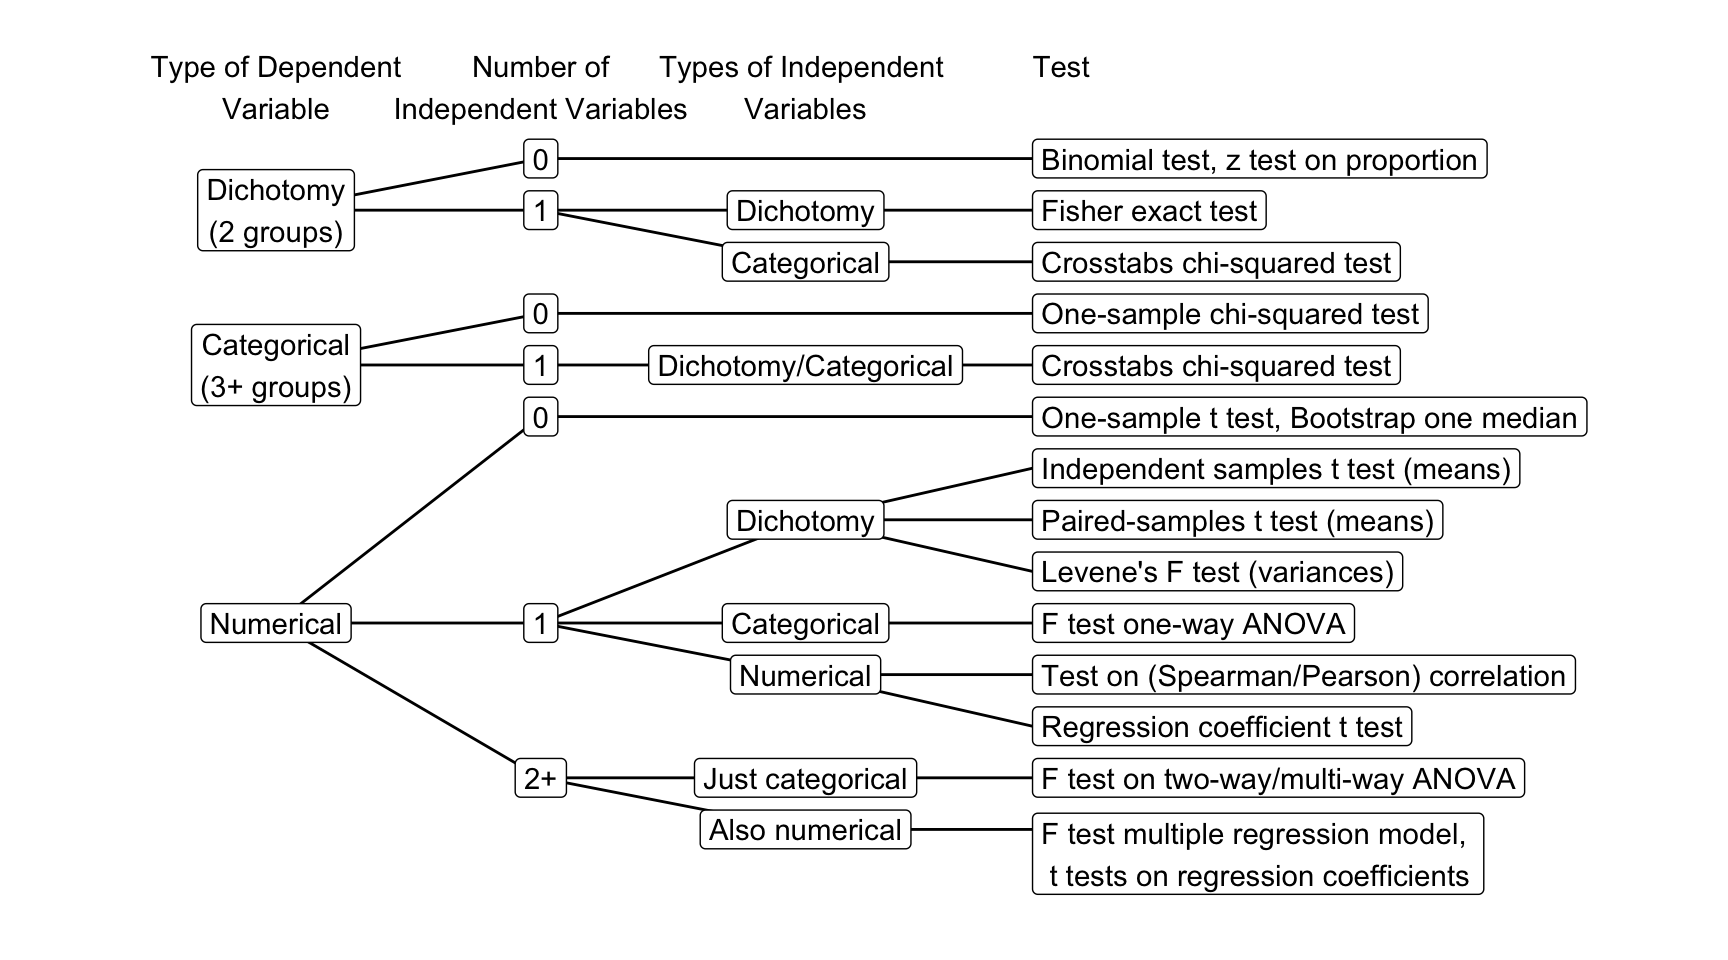
\includegraphics{GentleIntro_files/figure-latex/choice-diagram-copy-1.pdf}
\caption{\label{fig:choice-diagram-copy}Flow chart for selecting a test in
SPSS.}
\end{figure}

\subsubsection*{Chapter \ref{probmodels}: Probability Models: How Do I
Get a Sampling
Distribution?}\label{chapter-refprobmodels-probability-models-how-do-i-get-a-sampling-distribution}
\addcontentsline{toc}{subsubsection}{Chapter \ref{probmodels}:
Probability Models: How Do I Get a Sampling Distribution?}



Figure \ref{fig:SPSSbootstrap1}: Bootstrapping in SPSS.



Figure \ref{fig:SPSSbootstrap2}: Interpreting bootstrap results in SPSS.



Figure \ref{fig:SPSSExact1}: Performing an exact test in SPSS.



Figure \ref{fig:SPSSExact2}: Interpreting exact test results in SPSS.

\subsubsection*{Chapter \ref{param-estim}: Estimating a Parameter: Which
Population Values Are
Plausible?}\label{chapter-refparam-estim-estimating-a-parameter-which-population-values-are-plausible}
\addcontentsline{toc}{subsubsection}{Chapter \ref{param-estim}:
Estimating a Parameter: Which Population Values Are Plausible?}



Figure \ref{fig:SPSSconflevel}: Setting the confidence level in SPSS.

\subsubsection*{Chapter \ref{hypothesis}: Testing a Null Hypothesis: Am
I Right or Am I
Wrong?}\label{chapter-refhypothesis-testing-a-null-hypothesis-am-i-right-or-am-i-wrong}
\addcontentsline{toc}{subsubsection}{Chapter \ref{hypothesis}: Testing a
Null Hypothesis: Am I Right or Am I Wrong?}



Figure \ref{fig:SPSSbinomial}: A binomial test on a single proportion in SPSS.



Figure \ref{fig:SPSSchisq1}: A chi-squared test on a frequency distribution in SPSS.



Figure \ref{fig:SPSS1mean}: A one-sample t test in SPSS.

\subsubsection*{Chapter \ref{power}: Which Sample Size Do I Need?
Power!}\label{chapter-refpower-which-sample-size-do-i-need-power}
\addcontentsline{toc}{subsubsection}{Chapter \ref{power}: Which Sample
Size Do I Need? Power!}



Figure \ref{fig:cohend}: Calculating Cohen's d from SPSS output.

\subsubsection*{Chapter \ref{anova}: Moderation with Analysis of
Variance}\label{chapter-refanova-moderation-with-analysis-of-variance}
\addcontentsline{toc}{subsubsection}{Chapter \ref{anova}: Moderation
with Analysis of Variance}



Figure \ref{fig:SPSS1way}: One-way analysis of variance (ANOVA) in SPSS.



Figure \ref{fig:SPSS2way}: Two-way analysis of variance with moderation in SPSS.



Figure \ref{fig:SPSSeta2}: Calculating eta\textsuperscript{2} from SPSS output.

\subsubsection*{Chapter \ref{moderation}: Moderation with Regression
Analysis}\label{chapter-refmoderation-moderation-with-regression-analysis}
\addcontentsline{toc}{subsubsection}{Chapter \ref{moderation}:
Moderation with Regression Analysis}




Figure \ref{fig:SPSSregsimple}: Executing and interpreting regression analysis in
SPSS.



Figure \ref{fig:SPSSregdummy2}: Creating dummy variables in SPSS.



Figure \ref{fig:SPSSregdummy}: Using dummy variables in a regression model in SPSS.



Figure \ref{fig:SPSSreglines1}: Adding a regression line to a scatterplot in SPSS.



Figure \ref{fig:SPSSregassumpt}: Checking assumptions for regression models in SPSS.




Figure \ref{fig:SPSSregpred}: Creating categorical by continuous interaction
predictors for regression in SPSS.




Figure \ref{fig:SPSSregcatmod}: Estimating categorical by continuous moderation with
regression in SPSS.




Figure \ref{fig:SPSSregmodlines}: Representing moderation by regression lines in a
scatterplot in SPSS.




Figure \ref{fig:SPSSregSupport1}: Checking common support for a predictor at
different moderator values in SPSS.




Figure \ref{fig:SPSSregcenter}: Mean-centering variables for regression analysis in
SPSS.




Figure \ref{fig:SPSSreglines2}: Regression lines for a continuous moderator in a
scatterplot in SPSS.




Figure \ref{fig:SPSSregSupport2}: Checking common support with a continuous
moderator in SPSS.

\subsubsection*{Chapter \ref{mediation}: Mediation with Regression
Analysis}\label{chapter-refmediation-mediation-with-regression-analysis}
\addcontentsline{toc}{subsubsection}{Chapter \ref{mediation}: Mediation
with Regression Analysis}



Figure \ref{fig:SPSSregconfound}: Identifying confounders with regression in SPSS.




Figure \ref{fig:SPSSmediatpar}: Estimating a single or parallel mediation model with
PROCESS (Model 4).




Figure \ref{fig:SPSSmediatserial}: Estimating a serial mediation model with PROCESS
(Model 6).




Figure \ref{fig:SPSSmediatcov}: Estimating a mediation model including covariates
with PROCESS.



Figure \ref{fig:SPSSpath}: Estimating a path model in SPSS.

\chapter{Sampling Distribution: How Different Could My Sample Have
Been?}\label{samp-dist}

\begin{quote}
Key concepts: inferential statistics, generalization, population, random
sample, sample statistic, sampling space, random variable, sampling
distribution, probability, probability distribution, discrete
probability distribution, expected value/expectation, unbiased
estimator, parameter, (downward) biased, representative sample,
continuous variable, continuous probability distribution, probability
density, (left-hand/right-hand) p value.
\end{quote}

\subsection*{Summary}\label{summary}
\addcontentsline{toc}{subsection}{Summary}

\begin{quote}
What does our sample tell us about the population from which it was
drawn?
\end{quote}

Statistical inference is about estimation and null hypothesis testing.
We have collected data on a random sample and we want to draw
conclusions (make inferences) about the population from which the sample
was drawn. From the proportion of yellow candies in our sample bag, for
instance, we want to estimate a plausible range of values for the
proportion of yellow candies in a factory's stock (confidence interval).
Alternatively, we may want to test the null hypothesis that one fifth of
the candies in a factory's stock is yellow.

The sample does not offer a perfect miniature image of the population.
If we would draw another random sample, it would have different
characteristics. For instance, it would contain more or less yellow
candies than the previous sample. To make an informed decision on the
confidence interval or null hypothesis, we must compare the
characteristic of the sample that we have drawn to the characteristics
of the samples that we could have drawn.

The characteristics of the samples that we could have drawn is called
the sampling distribution. Sampling distributions are the central
element in estimation and null hypothesis testing. In this chapter, we
simulate sampling distributions to understand what they are. Here,
\emph{simulation} means that we let a computer draw many random samples
from a population.

In Communication Science, we usually work with samples of human beings,
for instance, users of social media, people looking for health
information or entertainment, citizens preparing to cast a political
vote, and an organization's stakeholders, or samples of media content
such as tweets, tv advertisements, or newspaper articles. In the current
and two subsequent chapters, however, we avoid the complexities of these
samples.

We focus on a very tangible kind of sample, namely a bag of candies,
which helps us understand the basic concepts of statistical inference:
sampling distributions (the current chapter), probability distributions
(Chapter \ref{probmodels}), and estimation (Chapter \ref{param-estim}).
Once we thoroughly understand these concepts, we turn to Communication
Science examples.

\section{Statistical Inference: Making the Most of Your
Data}\label{statistical-inference-making-the-most-of-your-data}

Statistics is a tool for scientific research. It offers a range of
techniques to check whether statements about the observable world
(empirical reality) are supported by data collected from that world.
Scientific theories strive for general statements, that is, statements
that apply to many situations. Checking these statements requires lots
of data covering all situations addressed by theory.

Collecting data, however, is expensive, so we would like to collect as
little data as possible and still be able to draw conclusions about a
much larger set. The cost and time involved in collecting large sets of
data are also relevant to applied research, such as market research. In
this context we also like to collect as little data as necessary.

\emph{Inferential statistics} offers techniques for making statements
about a larger set of observations from data collected for a smaller set
of observations. The large set of observations about which we want to
make a statement is called the \emph{population}. The smaller set is
called a \emph{sample}. We want to \emph{generalize} a statement about
the sample to a statement about the population from which the sample was
drawn.

Traditionally, statistical inference is generalization from the data
collected in a \emph{random sample} to the population from which the
sample was drawn. This approach is the focus of the present book because
it is currently the most widely used type of statistical inference in
the social sciences. We will, however, point out other approaches in
Chapter \ref{crit-discus}.

Statistical inference is conceptually complicated and for that reason
quite often used incorrectly. We will therefore spend quite some time on
the principles of statistical inference. Good understanding of the
principles should help you to recognize and avoid incorrect use of
statistical inference. In addition, it should help you to understand the
controversies surrounding statistical inference and developments in the
practice of applying statistical inference that are taking place.
Investing time and energy in fully understanding the principles of
statistical inference really pays off later.

\section{A Discrete Random Variable: How Many Yellow Candies in My
Bag?}\label{discreterandomvariable}

An obvious but key insight in statistical inference is this: If we draw
random samples from the same population, we are likely to obtain
different samples. No two random samples from the same population need
to be identical, even though they can be identical.

\subsection{Sample statistic}\label{sample-statistic}

We are usually interested in a particular characteristic of the sample
rather than in the exact nature of each observation within the sample.
For instance, I happen to be very fond of yellow candies. If I buy a bag
of candies, my first impulse is to tear the bag open and count the
number of yellow candies. Am I lucky today? Does my bag contain a lot of
yellow candies?

\begin{figure}[H]
\href{http://82.196.4.233:3838/apps/random-variable/}{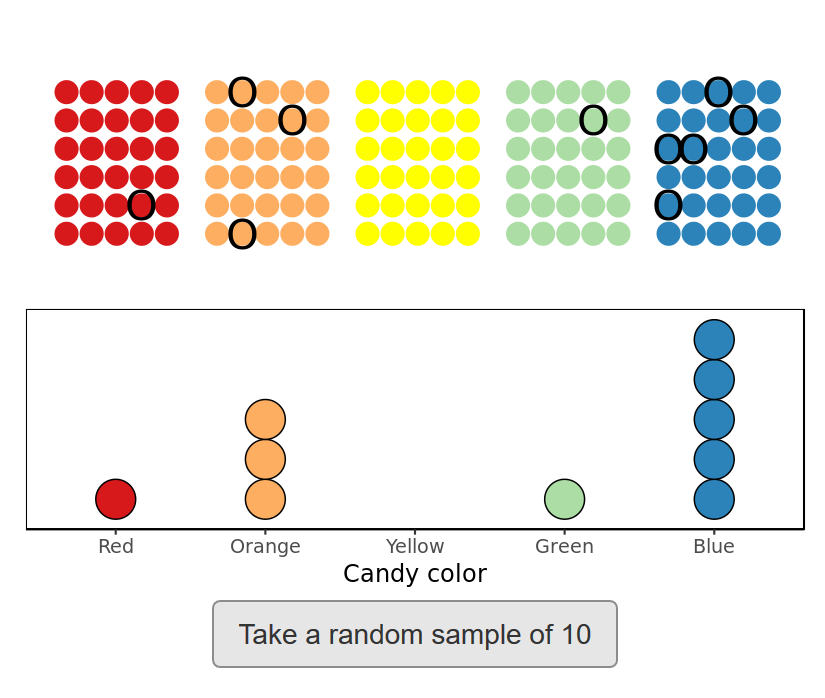
\includegraphics[width=420px]{GentleIntro_files/figure-latex/random-variable-1} }\caption{How many yellow candies will our sample bag contain?}\label{fig:random-variable}
\end{figure}

\begin{enumerate}
\def\labelenumi{\arabic{enumi}.}
\tightlist
\item
  Figure \ref{fig:random-variable} shows a population of candies. What
  do you expect is the number of yellow candies in a random sample of
  ten candies from this population? Draw several samples and check
  whether your expectation comes true.
\end{enumerate}

\begin{Shaded}
\begin{Highlighting}[]
\OperatorTok{*}\StringTok{ }\NormalTok{The colours are equally distributed }\ControlFlowTok{in}\NormalTok{ the population, so one out of each}
\NormalTok{five candies }\ControlFlowTok{in}\NormalTok{ the population is yellow. In other words, the proportion of}
\NormalTok{yellow candies }\ControlFlowTok{in}\NormalTok{ the population is .}\DecValTok{2}\NormalTok{.}
\OperatorTok{*}\StringTok{ }\NormalTok{This is the proportion that we would also expect }\ControlFlowTok{in}\NormalTok{ the sample. A sample}
\NormalTok{contains ten candies, so two out of these ten are expected to be yellow. If we}
\NormalTok{draw several samples, we notice that only a minority of our samples contain}
\NormalTok{exactly two yellow candies.}
\end{Highlighting}
\end{Shaded}

\begin{enumerate}
\def\labelenumi{\arabic{enumi}.}
\setcounter{enumi}{1}
\tightlist
\item
  What are all the possible outcomes for the number of yellow candies in
  our sample? The collection of all possible outcome scores is called
  the \emph{sampling space}.
\end{enumerate}

\begin{Shaded}
\begin{Highlighting}[]
\OperatorTok{*}\StringTok{ }\NormalTok{In a sample of ten candies, zero to ten candies can be yellow.}
\OperatorTok{*}\StringTok{ }\NormalTok{The numbers }\DecValTok{0}\NormalTok{, }\DecValTok{1}\NormalTok{, }\DecValTok{2}\NormalTok{, ..., }\DecValTok{9}\NormalTok{, }\DecValTok{10}\NormalTok{ constitute all possible outcomes }\ControlFlowTok{for}\NormalTok{ the}
\NormalTok{sample statistic }\StringTok{'Number of yellow candies'}\NormalTok{. This is called the sampling}
\NormalTok{space.}
\end{Highlighting}
\end{Shaded}

The number of yellow candies in a bag is an example of a \emph{sample
statistic}: a number describing a characteristic of the sample. Each
bag, that is, each sample, has one outcome score on the sample
statistic. For instance, one bag contains four yellow candies, another
bag contains seven, and so on.

The sample statistic is called a \emph{random variable}. It is a
variable because it assigns an outcome score to a sample and different
samples can have different scores. The value of a variable may vary from
sample to sample. It is a random variable because the score depends on
chance, namely the chance that particular elements are drawn during
random sampling.

\subsection{Sampling distribution}\label{sampling-distribution}

Some sample statistic outcomes occur more often than other outcomes. We
can see this if we draw very many random samples from a population and
collect the frequencies of all outcome scores in a table or chart. We
call the distribution of the outcome scores of very many samples a
\emph{sampling distribution}.

\begin{figure}[H]
\href{http://82.196.4.233:3838/apps/sampling-distribution/}{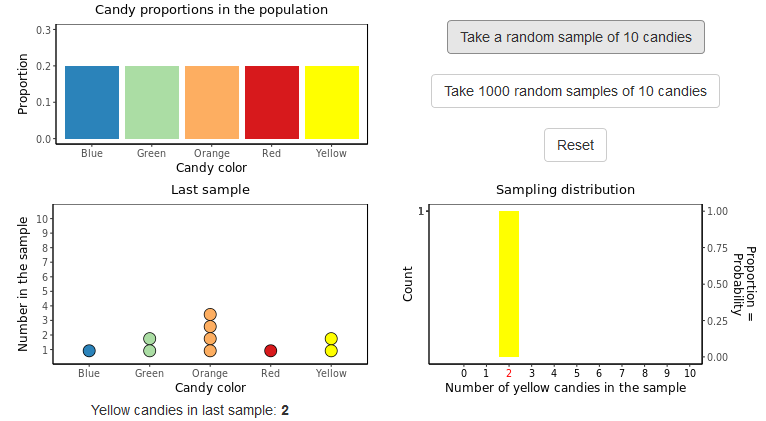
\includegraphics[width=420px]{GentleIntro_files/figure-latex/sampling-distribution-1} }\caption{What is a sampling distribution?}\label{fig:sampling-distribution}
\end{figure}

\begin{enumerate}
\def\labelenumi{\arabic{enumi}.}
\tightlist
\item
  Draw a random sample of ten candies in Figure
  \ref{fig:sampling-distribution}. What do the numbers on the horizontal
  axis of the bottom histograms mean? And what does the vertical axis of
  this histogram represent?
\end{enumerate}

\begin{Shaded}
\begin{Highlighting}[]
\OperatorTok{*}\StringTok{ }\NormalTok{The numbers on the horizontal axis constitute the sampling space, that is, all}
\NormalTok{values that the sample statistic }\StringTok{"Number of yellow candies"}\NormalTok{ can take.}
\OperatorTok{*}\StringTok{ }\NormalTok{The vertical axis shows the number of samples that have been drawn with a}
\NormalTok{particular value }\ControlFlowTok{for}\NormalTok{ the sample statistic, that is, with a particular number}
\NormalTok{of yellow candies }\ControlFlowTok{in}\NormalTok{ the sample.}
\end{Highlighting}
\end{Shaded}

\begin{enumerate}
\def\labelenumi{\arabic{enumi}.}
\setcounter{enumi}{1}
\tightlist
\item
  What are the cases (units of analysis) in the three histograms? Hint:
  There are two different types of cases.
\end{enumerate}

\begin{Shaded}
\begin{Highlighting}[]
\OperatorTok{*}\StringTok{ }\NormalTok{In the upper two graphs, candies are the cases. A candy has a particular}
\NormalTok{colour, not }\KeywordTok{a}\NormalTok{ (sample) bag of candies.}
\OperatorTok{*}\StringTok{ }\NormalTok{In the bottom graph showing the sampling distribution, }\KeywordTok{samples}\NormalTok{ (candy bags)}
\NormalTok{are the cases. A }\KeywordTok{sample}\NormalTok{ (bag) contains a particular number of yellow candies.}
\end{Highlighting}
\end{Shaded}

\begin{enumerate}
\def\labelenumi{\arabic{enumi}.}
\setcounter{enumi}{2}
\tightlist
\item
  Guess the most likely and most unlikely outcome scores for the number
  of yellow candies in a sample bag containing ten candies in Figure
  \ref{fig:sampling-distribution}. Check your intuitions by drawing
  1,000 samples.
\end{enumerate}

\begin{Shaded}
\begin{Highlighting}[]
\OperatorTok{*}\StringTok{ }\NormalTok{If twenty per cent of candies }\ControlFlowTok{in}\NormalTok{ the population are yellow, we expect about}
\NormalTok{twenty per cent of candies }\ControlFlowTok{in}\NormalTok{ our sample to be yellow. Our sample contains ten}
\NormalTok{candies, so we expect two yellow candies }\ControlFlowTok{in}\NormalTok{ our sample. Indeed, samples with}
\NormalTok{two yellow candies are most frequent }\ControlFlowTok{if}\NormalTok{ we draw }\DecValTok{1}\NormalTok{,}\DecValTok{000}\NormalTok{ random samples.}
\OperatorTok{*}\StringTok{ }\NormalTok{If we expect two candies, samples are more unlikely }\ControlFlowTok{if}\NormalTok{ they contain a number}
\NormalTok{of yellow candies that is further away from two. So we expect the sample}
\NormalTok{counts to decrease }\ControlFlowTok{if}\NormalTok{ we move away from two }\ControlFlowTok{in}\NormalTok{ the sampling distribution. Ten}
\NormalTok{yellow candies is furthest away from two }\ControlFlowTok{in}\NormalTok{ our sampling space, so a sample}
\NormalTok{bag with ten yellow candies is most unlikely.}
\end{Highlighting}
\end{Shaded}

\begin{enumerate}
\def\labelenumi{\arabic{enumi}.}
\setcounter{enumi}{3}
\tightlist
\item
  After how many samples does the shape of the sampling distribution
  stop changing?
\end{enumerate}

\begin{Shaded}
\begin{Highlighting}[]
\OperatorTok{*}\StringTok{ }\NormalTok{Theoretically, the sampling distribution represents an infinite number of}
\NormalTok{samples. In this example, the sampling distribution usually has its final}
\NormalTok{shape already after drawing }\DecValTok{1}\NormalTok{,}\DecValTok{000}\NormalTok{ or }\DecValTok{2}\NormalTok{,}\DecValTok{000}\NormalTok{ samples. But you can be unlucky, of}
\NormalTok{course, and need more samples to arrive at a stable distribution.}
\end{Highlighting}
\end{Shaded}

\subsection{Probability and probability
distribution}\label{probdistribution}

What is the probability of buying a bag with exactly five yellow
candies? In statistical terminology, what is the probability of drawing
a sample with five yellow candies as sample statistic outcome? This
probability is the proportion of all possible samples that we could have
drawn that happen to contain five yellow candies.

Of course, the probability of a sample bag with exactly five yellow
candies depends on the share of yellow candies in the population of all
candies. Figure \ref{fig:probability-distribution} displays the
probabilities of a sample bag with a particular number of yellow candies
if twenty per cent of the candies in the population are yellow. You can
adjust the population share of yellow candies to see what happens.

\begin{figure}[H]
\href{http://82.196.4.233:3838/apps/probability-distribution/}{\includegraphics[width=420px]{GentleIntro_files/figure-latex/probability-distribution-1} }\caption{How does the probability of drawing a sample bag with two out of ten candies yellow depend on the proportion of yellow candies in the population?}\label{fig:probability-distribution}
\end{figure}

\begin{enumerate}
\def\labelenumi{\arabic{enumi}.}
\tightlist
\item
  In Figure \ref{fig:probability-distribution}, what is the sample
  statistic and what is the sampling space?
\end{enumerate}

\begin{Shaded}
\begin{Highlighting}[]
\OperatorTok{*}\StringTok{ }\NormalTok{The number of yellow candies }\ControlFlowTok{in}\NormalTok{ the }\KeywordTok{sample}\NormalTok{ (bag) is the sample statistic.}
\NormalTok{This is the characteristic of the }\KeywordTok{sample}\NormalTok{ (bag) that we are interested in.}
\OperatorTok{*}\StringTok{ }\NormalTok{The set of all possible outcomes of the sample statistic is the sampling}
\NormalTok{space. In this example, the sampling space is the set }\KeywordTok{of}\NormalTok{ (integer) numbers}
\NormalTok{from }\DecValTok{0}\NormalTok{ to }\DecValTok{10}\NormalTok{.}
\end{Highlighting}
\end{Shaded}

\begin{enumerate}
\def\labelenumi{\arabic{enumi}.}
\setcounter{enumi}{1}
\tightlist
\item
  Which number of yellow candies is most likely to be found in a sample
  bag of ten candies? How does this relate to the proportion of candies
  in the population?
\end{enumerate}

\begin{Shaded}
\begin{Highlighting}[]
\OperatorTok{*}\StringTok{ }\NormalTok{The numbers and horizontal bars }\ControlFlowTok{in}\NormalTok{ the Probability column represent the}
\NormalTok{probabilities of outcomes. In the initial situation, the highest probability}
\NormalTok{is found }\ControlFlowTok{for}\NormalTok{ a sample bag containing two yellow }\KeywordTok{candies}\NormalTok{ (}\DataTypeTok{p =}\NormalTok{ .}\DecValTok{302}\NormalTok{). This}
\NormalTok{amounts to two out of the ten candies }\ControlFlowTok{in}\NormalTok{ the sample bag, that is, twenty per}
\NormalTok{cent.}
\OperatorTok{*}\StringTok{ }\NormalTok{This percentage is equal to the precentage of yellow candies }\ControlFlowTok{in}\NormalTok{ the}
\NormalTok{population. We are most likely to draw a sample with a percentage or}
\NormalTok{proportion that is equal to the population percentage, here p =}\StringTok{ }\NormalTok{.}\DecValTok{302}\NormalTok{, even}
\NormalTok{though the total probability of drawing a sample with another percentage of}
\NormalTok{yellow candies is }\KeywordTok{higher}\NormalTok{ (}\DataTypeTok{p =} \DecValTok{1} \OperatorTok{-}\StringTok{ }\DataTypeTok{.302 =}\NormalTok{ .}\DecValTok{698}\NormalTok{).}
\end{Highlighting}
\end{Shaded}

\begin{enumerate}
\def\labelenumi{\arabic{enumi}.}
\setcounter{enumi}{2}
\tightlist
\item
  What is the probability that a sample bag of ten candies contains not
  more than three yellow candies if the proportion in the population is
  .2?
\end{enumerate}

\begin{Shaded}
\begin{Highlighting}[]
\OperatorTok{*}\StringTok{ }\NormalTok{At most three out of ten candies means that we have to sum the probabilities}
\NormalTok{of zero, one, two, and three yellow candies. This probability equals .}\DecValTok{107} \OperatorTok{+}
\NormalTok{.}\DecValTok{268} \OperatorTok{+}\StringTok{ }\NormalTok{.}\DecValTok{302} \OperatorTok{+}\StringTok{ }\NormalTok{.}\DecValTok{201}\NormalTok{ =}\StringTok{ }\NormalTok{.}\DecValTok{878}\NormalTok{. That is a fair chance.}
\end{Highlighting}
\end{Shaded}

\begin{enumerate}
\def\labelenumi{\arabic{enumi}.}
\setcounter{enumi}{3}
\tightlist
\item
  What do you expect to happen to the probabilities if you increase the
  proportion of yellow candies in the population (factory stock)? Use
  the slider to check your answer.
\end{enumerate}

\begin{Shaded}
\begin{Highlighting}[]
\OperatorTok{*}\StringTok{ }\NormalTok{If a larger part of the candies is yellow }\ControlFlowTok{in}\NormalTok{ the population, we should}
\NormalTok{expect more yellow candies }\ControlFlowTok{in}\NormalTok{ our sample bag. The probabilities of small}
\NormalTok{numbers of yellow }\KeywordTok{candies}\NormalTok{ (low outcome values) should go down whereas the}
\NormalTok{probabilities of large }\KeywordTok{numbers}\NormalTok{ (high outcome scores) should go up.}
\OperatorTok{*}\StringTok{ }\NormalTok{If you move the slider to the right, you will see that the distribution}
\NormalTok{shifts down }\ControlFlowTok{in}\NormalTok{ the table.}
\end{Highlighting}
\end{Shaded}

\begin{enumerate}
\def\labelenumi{\arabic{enumi}.}
\setcounter{enumi}{4}
\tightlist
\item
  What is special about the distribution if the proportion of yellow
  candies in the population is .5?
\end{enumerate}

\begin{Shaded}
\begin{Highlighting}[]
\OperatorTok{*}\StringTok{ }\NormalTok{If the population proportion is .}\DecValTok{5}\NormalTok{, the probability distribution is}
\NormalTok{symmetric. The probability of a sample bag with four candies is equal to the}
\NormalTok{probability of a sample bag with six candies. Probabilities are equal }\ControlFlowTok{for}
\NormalTok{three and seven yellow candies, two and eight, one and nine, zero and ten}
\NormalTok{yellow candies.}
\OperatorTok{*}\StringTok{ }\NormalTok{The distribution has the classic symmetric bell shape of a normal}
\NormalTok{distribution that we will encounter when we discuss continuous probability}
\NormalTok{distributions.}
\end{Highlighting}
\end{Shaded}

The sampling distribution tells us all possible samples that we could
have drawn, that is, if we have drawn very many samples. We can use the
distribution of all samples to get the probability of buying a bag with
exactly five yellow candies from the sampling distribution: We merely
divide the number of samples with five yellow candies by the total
number of samples we have drawn.

If we change the (absolute) frequencies in the sampling distribution
into proportions (relative frequencies), we obtain the \emph{probability
distribution} of the sample statistic: A sampling space with a
probability (between 0 and 1) for each outcome of the sample statistic.
Because we are usually interested in probabilities, sampling
distributions tend to have proportions, that is probabilities, instead
of frequencies on the vertical axis. See Figure \ref{fig:expected-value}
for an example. In this case, the sampling distribution is a probablity
distribution.

Figure \ref{fig:probability-distribution} displays the probability
distribution of the number of yellow candies per bag of ten candies.
This is an example of a \emph{discrete probability distribution} because
only a limited number of outcomes are possible. It is feasible to list
the probability of each outcome separately.

The sampling distribution as a probability distribution conveys very
important information. It tells us which outcomes we can expect, in our
example, how many yellow candies we may find in our bag of ten candies.
Moreover, it tells us the probability that a particular outcome may
occur. If the sample is drawn from a population in which twenty per cent
of candies are yellow, we are quite likely to find zero, one, two,
three, or four yellow candies in our bag. A bag with five yellow candies
would be rare, six or seven candies would be very rare, and a bag with
more than seven yellow candies is extremely unlikely but not impossible.
If we buy such a bag, we know that we have been extremely lucky.

We may refer to probabilities both as a proportion, that is, a number
between 0 and 1, and as a percentage: a number between 0\% and 100\%.
Proportions are commonly considered to be the correct way to express
probabilities. When we talk about probabilities, however, we tend to use
percentages; we may, for example, say that the probabilities are
fifty-fifty.

\subsection{Expected value or expectation}\label{expectedvalue}

We haven't yet thought about the value that we are most likely to
encounter in the sample that we are going to draw. Intuitively, it must
be related to the distribution of colours in the population of candies
from which the sample was drawn. In other words, the share of yellow
candies in the factory's stock from which the bag was filled or in the
machine that produces the candies, seems to be relevant to what we may
expect to find in our sample.

\begin{figure}[H]
\href{http://82.196.4.233:3838/apps/expected-value/}{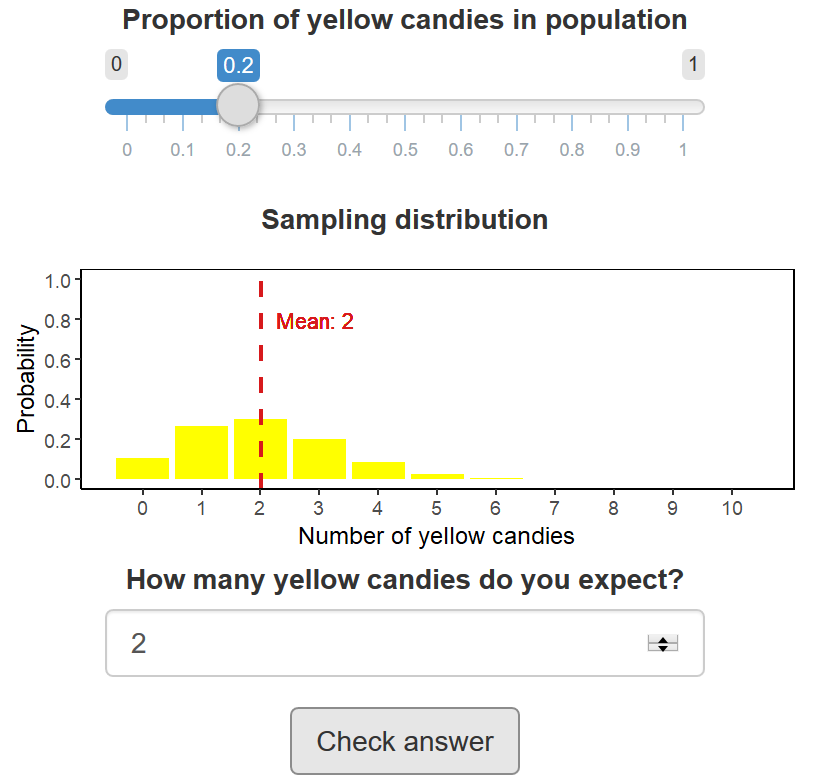
\includegraphics[width=420px]{GentleIntro_files/figure-latex/expected-value-1} }\caption{What is the expected value of a probability distribution?}\label{fig:expected-value}
\end{figure}

\begin{enumerate}
\def\labelenumi{\arabic{enumi}.}
\tightlist
\item
  In Figure \ref{fig:expected-value}, which number of yellow candies is
  most likely to occur in a sample bag of ten candies? How does this
  number change if you change the proportion of yellow candies in the
  population?
\end{enumerate}

\begin{Shaded}
\begin{Highlighting}[]
\OperatorTok{*}\StringTok{ }\NormalTok{We expect that the proportion of yellow candies }\ControlFlowTok{in}\NormalTok{ the sample equals the}
\NormalTok{population proportion, which initially is .}\DecValTok{2}\NormalTok{. In a sample of ten candies,}
\NormalTok{then, the expected number of yellow candies is two.}
\OperatorTok{*}\StringTok{ }\NormalTok{Note that two is the outcome with the highest probability }\ControlFlowTok{in}\NormalTok{ the sampling}
\NormalTok{distribution.}
\OperatorTok{*}\StringTok{ }\NormalTok{The expected number of yellow candies }\ControlFlowTok{in}\NormalTok{ a sample bag of ten candies is ten}
\NormalTok{times the population proportion, so the expected number of candies }\ControlFlowTok{in}\NormalTok{ the}
\NormalTok{sample changes }\ControlFlowTok{in}\NormalTok{ accordance with changes }\ControlFlowTok{in}\NormalTok{ the population proportion.}
\end{Highlighting}
\end{Shaded}

\begin{enumerate}
\def\labelenumi{\arabic{enumi}.}
\setcounter{enumi}{1}
\tightlist
\item
  How does the mean of the sampling distribution relate to the expected
  value? Experiment with different values for the population proportion.
\end{enumerate}

\begin{Shaded}
\begin{Highlighting}[]
\OperatorTok{*}\StringTok{ }\NormalTok{The mean of the sampling distribution is equal to the expected value of the}
\NormalTok{sample statistic. In the initial example, both are two.}
\OperatorTok{*}\StringTok{ }\NormalTok{This makes sense}\OperatorTok{:}\StringTok{ }\NormalTok{Samples with fewer yellow candies than expected should}
\NormalTok{balance samples with more yellow candies than expected. The mean represents the}
\StringTok{"balance point"}\NormalTok{ of a distribution.}
\end{Highlighting}
\end{Shaded}

\begin{enumerate}
\def\labelenumi{\arabic{enumi}.}
\setcounter{enumi}{2}
\tightlist
\item
  How does the mean of the sampling distribution relate to the
  population proportion? Experiment with different values for the
  population proportion.
\end{enumerate}

\begin{Shaded}
\begin{Highlighting}[]
\OperatorTok{*}\StringTok{ }\NormalTok{The mean of the sampling distribution of the sample proportion is equal to}
\NormalTok{the population proportion. If we would have created the sampling distribution}
\NormalTok{of the proportion of yellow candies }\ControlFlowTok{in}\NormalTok{ our sample, the mean of the sampling}
\NormalTok{distribution would be equal to the proportion of yellow candies }\ControlFlowTok{in}\NormalTok{ the}
\NormalTok{population.}
\OperatorTok{*}\StringTok{ }\NormalTok{Again, we are equally likely to draw a sample with less yellow candies than}
\NormalTok{the expected proportion as a sample with more yellow candies. Samples with}
\NormalTok{less yellow candies than expected should balance samples with more yellow}
\NormalTok{candies than expected. The mean represents the }\StringTok{"balance point"}\NormalTok{ of a}
\NormalTok{distribution.}
\OperatorTok{*}\StringTok{ }\NormalTok{Note that the expected }\KeywordTok{value}\NormalTok{ (mean of the sampling distribution) only equals}
\NormalTok{the population value }\ControlFlowTok{if}\NormalTok{ the sample statistic is an unbiased estimate of the}
\NormalTok{population }\KeywordTok{value}\NormalTok{ (parameter). See the }\ControlFlowTok{next}\NormalTok{ section.}
\end{Highlighting}
\end{Shaded}

If the share of yellow candies in the population is 0.20 (or 20\%), we
expect one out of each five candies in a bag (sample) to be yellow. In a
bag with 10 candies, we would expect two candies to be yellow: one out
of each five candies or the population proportion times the total number
of candies in the sample = 0.20 * 10 = 2.0. This is the expected value.

The expected value of the proportion of yellow candies in the sample is
equal to the proportion of yellow candies in the population. If you
carefully inspect a sampling distribution (Figure
\ref{fig:expected-value}), you will see that the expected value also
equals the mean of the sampling distribution. This makes sense: Excess
yellow candies in some bags must be compensated for by a shortage in
other bags.

Thus we arrive at the definition of the \emph{expected value} of a
random variable:

\begin{quote}
The expected value is the average of the sampling distribution of a
random variable.
\end{quote}

In our example, the random variable is a sample statistic, more
specifically, the number of yellow candies in a sample.

The sampling distribution is an example of a probability distribution,
so, more generally, the expected value is the average of a probability
distribution. The expected value is also called the \emph{expectation}
of a probability distribution.

\subsection{Unbiased estimator}\label{unbiased-est}

Note that the expected value of the proportion of yellow candies in the
bag (sample statistic) equals the true proportion of yellow candies in
the candy factory (population statistic). This is always, that is, by
definition, true for all sample statistics that are \emph{unbiased
estimators} of the population statistic. By the way, we usually refer to
the population statistic as a \emph{parameter}.

Most but not all sample statistics are unbiased estimators of the
population statistic. Think, for instance, of the actual number of
yellow candies in the sample. This is certainly not an unbiased
estimator of the number of yellow candies in the population. Because the
population is so much larger than the sample, the population must
contain many more yellow candies than the sample. If we were to estimate
the number in the population (the parameter) from the number in the
sample---for instance, we estimate that there are two yellow candies in
the population of all candies because we have two in our sample of
ten---we are going to vastly underestimate the number in the population.
This estimate is \emph{downward biased}: It is too low.

In contrast, the proportion in the sample is an unbiased estimator of
the population proportion. That is why we do not use the number of
yellow candies to generalize from our sample to the population. Instead,
we use the proportion of yellow candies. You probably already did this
intuitively.

Sometimes, we have to adjust the way in which we calculate a sample
statistic to get an unbiased estimator. For instance, we must calculate
the standard deviation and variance in the sample in a special way to
obtain an unbiased estimate of the population standard deviation and
variance. The exact calculation need not bother us, because our
statistical software will take care of that.

\subsection{Representative sample}\label{representative}

Because the share of yellow candies in the population represents the
probability of drawing a yellow candy, we also expect 20\% of the
candies in our bag to be yellow. For the same reason we expect the
shares of all other colours in our sample bag to be equal to their
shares in the population. As a consequence, we expect a random sample to
resemble the population from which it is drawn.

A sample is \emph{representative} of a population if variables in the
sample are distributed in the same way as in the population. Of course,
we know that a random sample is likely to differ from the population due
to chance, so the actual sample that we have drawn is usually not
representative of the population.

But we should expect it to be representative, so we say that it is
\emph{in principle representative} of the population. We can use
probability theory to account for the misrepresentation in the actual
sample that we draw. This is what we do when we use statistical
inference to construct confidence intervals and test null hypotheses.

\section{A Continuous Random Variable: Overweight And
Underweight.}\label{cont-random-var}

Let us now look at another variable: the weight of candies in a bag. The
weight of candies is perhaps more interesting to the average consumer
than candy colour because candy weight is related to calories.

\subsection{Continuous variable}\label{continuous-variable}

Weight is a \emph{continuous variable} because we can always think of a
new weight between two other weights. For instance, consider two candy
weights: 2.8 and 2.81 gram. It is easy to see that there can be a weight
in between these two values, for instance, 2.803 gram. Between 2.8 and
2.803 we can discern an intermediate value such as 2.802. In principle,
we could continue doing this endlessly, e.g., find a weight between
2.80195661 and 2.80195662 gram even if our scales may not be
sufficiently precise to measure any further differences. It is the
principle that counts. If we can always think of a new value in between
two values, the variable is continuous.

\subsection{Continuous sample statistic}\label{cont_sample_stat}

We are not interested in the weight of a single candy. If a relatively
light candy is compensated for by a relatively heavy candy in the same
bag, we still get the calories that we want. We are interested in the
average weight of all candies in our sample bag, so average candy weight
in our sample bag is our key sample statistic. We want to use this
sample statistic to say something about average candy weight in the
population of all candies. Can we do that?

The sample mean is an unbiased estimator of the population mean, so the
average weight of all candies in the population (at the factory) is the
average of the (candy weights in the) sampling distribution. And this is
the average weight that we expect in a sample drawn from this population
(the expected value or expectation). So far, everything is the same as
in the case of the number of yellow candies in the sample, which was a
discrete random variable because it could take only a limited set of
values: 0 to 10.

\subsection{Continuous probabilities}\label{continuous-probabilities}

When we turn to the probabilities of getting samples with a particular
average candy weight, we run into problems with a continuous sample
statistic. If we would want to know the probability of drawing a sample
bag with an average candy weight of 2.8 gram, we should exclude sample
bags with an average candy weight of 2.81 gram, or 2.801 gram, or
2.8000000001 gram, and so on. In fact, we are very unlikely to draw a
sample bag with an average candy weight of exactly 2.8 gram, that is,
with an infinite number of zeros trailing 2.8. In other words, the
probability of such a sample bag is for all practical purposes zero and
negligible.

This applies to every average candy weight, so all probabilities are
virtually zero. The probability distribution of the sampling space, that
is, of all possible outcomes, is going to be very boring: just (nearly)
zeros. And it will take forever to list all possible outcomes within the
sampling space, because we have an infinite number of possible outcomes.
After all, we can always find a new average candy weight between two
selected weights.

\subsection{p Values}\label{p-values}

We can solve this problem by looking at a range of values instead of a
single value. We can meaningfully talk about the probability of having a
sample bag with an average candy weight of at least 2.8 gram or at most
2.8 gram. We choose a threshold, in this example 2.8 gram, and determine
the probability of values above or below this threshold. We can also use
two thresholds, for example the probability of an average candy weight
between 2.75 and 2.85 gram. This is probably what you were thinking of
when I referred to a bag with 2.8 gram as average candy weight.

If we cannot determine the probability of a single value, which we used
to depict on the vertical axis, and we have to link probabilities to a
range of values on the x axis, for example, average candy weight
above/below 2.8 gram, how can we display probabilities? We have to
display a probability as an area between the horizontal axis and a
curve. This curve is called a \emph{probability density function}, so if
there is a label to the vertical axis of a continuous probability
distribution, it usually is ``Probability density'' instead of
``Probability''.

Figure \ref{fig:p-values} shows an example of a continuous probability
distribution for the average weight of candies in a sample bag. This is
the familiar normal distribution so we could say that the normal
function is the probability density function here. The total area under
this curve is set to one, so the area belonging to a range of sample
outcomes (average candy weight) is 1 or less, as probabilities should
be.

\begin{figure}[H]
\href{http://82.196.4.233:3838/apps/p-values/}{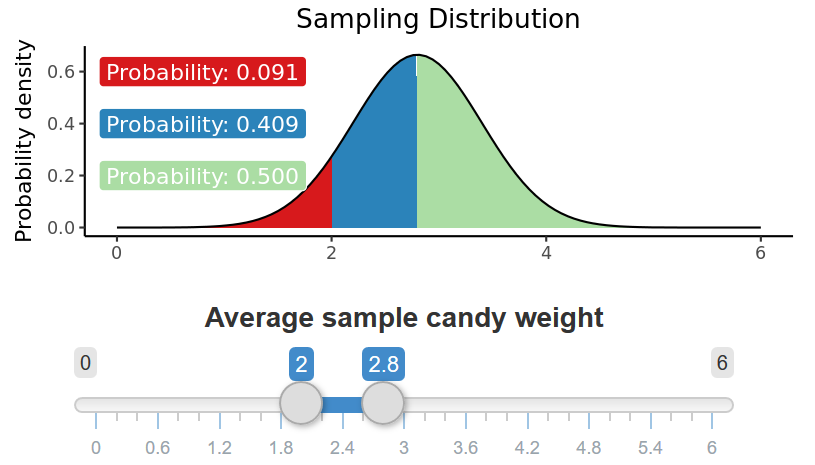
\includegraphics[width=420px]{GentleIntro_files/figure-latex/p-values-1} }\caption{How do we display probabilities in a continuous sampling distribution? Tip: Click on a slider handle and use your keyboard arrow keys to make small changes to the slider handle position.}\label{fig:p-values}
\end{figure}

\begin{enumerate}
\def\labelenumi{\arabic{enumi}.}
\tightlist
\item
  In Figure \ref{fig:p-values}, what is the probability of buying a bag
  with average candy weight of 2.8 gram or more?
\end{enumerate}

\begin{Shaded}
\begin{Highlighting}[]
\OperatorTok{*}\StringTok{ }\NormalTok{The probability is .}\DecValTok{5}\NormalTok{. It is represented by the green surface under the}
\NormalTok{curve. This is exactly half of the total surface under the curve because }\FloatTok{2.8}
\NormalTok{gram is the average candy weight }\ControlFlowTok{in}\NormalTok{ the population and, as a result, the}
\NormalTok{average value of the sampling distribution of average sample candy weight.}
\end{Highlighting}
\end{Shaded}

\begin{enumerate}
\def\labelenumi{\arabic{enumi}.}
\setcounter{enumi}{1}
\tightlist
\item
  What do you think, is this a left-hand probability or a right-hand
  probability?
\end{enumerate}

\begin{Shaded}
\begin{Highlighting}[]
\OperatorTok{*}\StringTok{ }\NormalTok{This is a right}\OperatorTok{-}\NormalTok{hand probability because it specifies a threshold value}
\NormalTok{(}\FloatTok{2.8}\NormalTok{) and all values that are larger. It concerns the right}\OperatorTok{-}\NormalTok{hand tail of the}
\NormalTok{sampling distribution.}
\end{Highlighting}
\end{Shaded}

\begin{enumerate}
\def\labelenumi{\arabic{enumi}.}
\setcounter{enumi}{2}
\tightlist
\item
  Use the sliders to find the probability of buying a bag with average
  candy weight between 2.6 and 3.7 gram. Is this a left-hand
  probability, a right-hand probability, or neither?
\end{enumerate}

\begin{Shaded}
\begin{Highlighting}[]
\OperatorTok{*}\StringTok{ }\NormalTok{If you set the slider handles to }\FloatTok{2.6}\NormalTok{ and }\FloatTok{3.7}\NormalTok{, the blue area represents the}
\NormalTok{probability that you are looking for. Its value is reported as .}\DecValTok{564}\NormalTok{.}
\OperatorTok{*}\StringTok{ }\NormalTok{This is neither a left}\OperatorTok{-}\NormalTok{hand or right}\OperatorTok{-}\NormalTok{hand probability because it does not}
\NormalTok{include either the left}\OperatorTok{-}\NormalTok{hand or right}\OperatorTok{-}\NormalTok{hand tail of the sampling distribution.}
\end{Highlighting}
\end{Shaded}

\begin{enumerate}
\def\labelenumi{\arabic{enumi}.}
\setcounter{enumi}{3}
\tightlist
\item
  What is the minimum average weight of the 10\% heaviest candy bags?
\end{enumerate}

\begin{Shaded}
\begin{Highlighting}[]
\OperatorTok{*}\StringTok{ }\NormalTok{Drag the right}\OperatorTok{-}\NormalTok{hand slider handle to the maximum }\KeywordTok{value}\NormalTok{ (}\DecValTok{6}\NormalTok{) and then adjust}
\NormalTok{the left}\OperatorTok{-}\NormalTok{hand slider handle so }\KeywordTok{the}\NormalTok{ (blue) area }\ControlFlowTok{in}\NormalTok{ the right}\OperatorTok{-}\NormalTok{tail of the}
\NormalTok{sampling distribution represent a probability of .}\DecValTok{100}\NormalTok{. This area contains the}
\NormalTok{ten per cent samples with largest average candy weight scores. The value}
\NormalTok{displayed with the left}\OperatorTok{-}\NormalTok{hand }\KeywordTok{slider}\NormalTok{ (}\FloatTok{3.57}\NormalTok{) is the minimum average candy weight}
\NormalTok{of the }\DecValTok{10}\NormalTok{% heaviest candy bags.}
\end{Highlighting}
\end{Shaded}

The probability of values up to (and including) the threshold value or
the threshold value and higher are called \emph{p values}. The
probability of values up to (and including) the threshold value is known
as the \emph{left-hand p value} and the probability of values above (and
including) the threshold value is called the \emph{right-hand p value}.

Why did I put \emph{(and including)} between parentheses? It does not
really matter whether we add the exact boundary value (2.8 gram) to the
probability on the left or on the right because the probability of
getting a bag with average candy weight at exactly 2.8 gram (with a very
long trail of zero decimals) is negligible.

Are you struggling with the idea of areas instead of heights (values on
the vertical axis) as probabilities? Just consider the idea that we
could use the area of a bar in a histogram instead of the height as
indication of the probability in discrete probability distrbutions, for
example, Figure \ref{fig:expected-value}. After all, the bars in a
histogram are all equally wide, so differences between bar areas are
proportional to differences in bar height.

\subsection{Probabilities always sum to
1}\label{probabilities-always-sum-to-1}

While you were playing with Figure \ref{fig:p-values}, you may have
noticed that displayed probabilities always add up to one. This is true
for every probability distribution because it is part of the definition
of a probability distribution. In addition, you may have realized that
we can use probability distributions in two ways. We can use them to say
how likely or unlikely we are to draw a sample with the sample statistic
value in a particular range. For example, what is the chance that we
draw a sample bag with average candy weight over 2.9 gram? But we can
also use a probability distribution to find the threshold values that
separate the top ten per cent or the bottom five per cent in a
distribution. If we want a sample bag with highest average candy weight,
say, belonging to the ten per cent bags with highest average candy
weight, what should be the average candy weight in the sample bag?

\section{Concluding Remarks}\label{concluding-remarks}

A communication scientist wants to know whether children are
sufficiently aware of the dangers of media use. On a media literacy
scale from one to ten, an average score of 5.5 or higher is assumed to
be sufficient.

If we translate this to the simple candy bag example, we realize that
the outcome in our sample need not be the true population value. After
all, we could very well draw a bag with less or more than twenty per
cent yellow candies.

Average media literacy, then, can exceed 5.5 in our sample of children,
even if average media literacy is below 5.5 in the population or the
other way around. How we decide on this is discussed in later chapters.

\subsection{Samples characteristics as
observations}\label{samples-characteristics-as-observations}

Perhaps the most confusing aspect of sampling distributions is the fact
that samples are our cases (units of analysis) and sample
characteristics are our observations. We are accustomed to think of
observations as measurements on empirical \emph{things} such as people
or candies. We perceive each person or each candy as a case and we
observe a characteristic that may change across cases (a variable), for
instance the colour or weight of a candy.

In a sampling distribution, however, we observe samples (cases) and
measure a sample statistic as the (random) variable. Each sample adds
one observation to the sampling distribution and its sample statistic
value is the value added to the sampling distribution.

\subsection{Means at three levels}\label{means-at-three-levels}

In our first example, the sample statistic is a proportion, namely the
proportion of candies that are yellow. The horizontal axis of the
sampling distribution represents the proportion of yellow candies. This
is fully in line with our research question. If we want to know whether
all colours are equally distributed, we are interested in sample
proportions, not in properties of individual candies.

Things become a little confusing if we are interested in a sample mean,
such as the average weight of candies in a sample bag. Now we have means
at three levels: the population, the sampling distribution, and the
sample.

\begin{figure}[H]
\href{http://82.196.4.233:3838/apps/three-means/}{\includegraphics[width=420px]{GentleIntro_files/figure-latex/three-means-1} }\caption{What is the relation between the three distributions?}\label{fig:three-means}
\end{figure}

\begin{enumerate}
\def\labelenumi{\arabic{enumi}.}
\tightlist
\item
  In Figure \ref{fig:three-means}, explain the meaning of the three
  means (dotted red lines). Which mean is a mean of means?
\end{enumerate}

\begin{Shaded}
\begin{Highlighting}[]
\OperatorTok{*}\StringTok{ }\NormalTok{The dotted red line }\ControlFlowTok{in}\NormalTok{ the top graph represents the average of candy weights}
\ControlFlowTok{in}\NormalTok{ the population.}
\OperatorTok{*}\StringTok{ }\NormalTok{The dotted red line }\ControlFlowTok{in}\NormalTok{ the middle graph represents the average of sampling}
\NormalTok{means. So it is the average of average candy weight }\ControlFlowTok{in}\NormalTok{ a sample. It is a mean}
\NormalTok{of means.}
\OperatorTok{*}\StringTok{ }\NormalTok{The dotted red line }\ControlFlowTok{in}\NormalTok{ the bottom graph represents the average of candy}
\NormalTok{weights }\ControlFlowTok{in}\NormalTok{ the sample.}
\end{Highlighting}
\end{Shaded}

\begin{enumerate}
\def\labelenumi{\arabic{enumi}.}
\setcounter{enumi}{1}
\tightlist
\item
  Is it a coincidence that the mean of the population and sampling
  distribution are the same? Use a slider to check if these means are
  the same.
\end{enumerate}

\begin{Shaded}
\begin{Highlighting}[]
\OperatorTok{*}\StringTok{ }\NormalTok{This is not a coincidence because the population mean is the expected value}
\NormalTok{of the sampling distribution and the expected value of the sampling}
\NormalTok{distribution is the average of the sampling distribution.}
\end{Highlighting}
\end{Shaded}

\begin{enumerate}
\def\labelenumi{\arabic{enumi}.}
\setcounter{enumi}{2}
\tightlist
\item
  How does the sample mean relate to the population mean and the mean of
  the sampling distribution?
\end{enumerate}

\begin{Shaded}
\begin{Highlighting}[]
\OperatorTok{*}\StringTok{ }\NormalTok{The sample mean is one of the sample means included }\ControlFlowTok{in}\NormalTok{ the sampling}
\NormalTok{distribution. The sample is, so to speak, one of the possible samples that are}
\NormalTok{listed }\ControlFlowTok{in}\NormalTok{ the sampling distribution.}
\OperatorTok{*}\StringTok{ }\NormalTok{The sampling distribution depends on the population distribution. For}
\NormalTok{instance, the mean or centre of the sampling distribution of sample means}
\NormalTok{equals the population }\KeywordTok{mean}\NormalTok{ (because the sample mean is an unbiased estimator}
\NormalTok{of the population mean).}
\OperatorTok{*}\StringTok{ }\NormalTok{If the population changes, the sampling distribution changes, so the list of}
\NormalTok{possible }\KeywordTok{samples}\NormalTok{ (better}\OperatorTok{:}\StringTok{ }\NormalTok{the probabilities of sample outcomes) changes, so we}
\NormalTok{expect a different sample. But this sample need not have the same mean as the}
\NormalTok{population and the sampling distribution because it is drawn at random. The}
\NormalTok{sample mean is more likely to be close to than very distant from the}
\NormalTok{population mean but it still can be quite different from the population mean.}
\end{Highlighting}
\end{Shaded}

The sampling distribution, here, is a distribution of sample means but
the sampling distribution itself also has a mean, which is called the
expected value or expectation of the sampling distribution. Don't get
confused about this. The mean of the sampling distribution is the
average of the average weight of candies across all possible sample
bags. This mean of means has the same value as our first mean, namely
the average weight of the candies in the population because a sample
mean is an unbiased estimator of the population mean.

Think of the three distributions as a hamburger. The top and bottom part
of a hamburger are both made of bread. They represent the population and
the sample, which consist of the same substance: candies and their
weight in our example. The middle part of the hamburger, however, is a
completely different type of food. The meat holds the two halves of the
bun together. In a similar way, the sampling distribution connects the
population to the sample but it is of a very different substance. It
consists of samples, for instance, bags of candies instead of single
candies.

The sampling distribution sticks to the population because the
population statistic (parameter), for example, the average weight of all
candies, is equal to the mean of the sampling distribution. The sampling
distribution sticks to the sample because it tells us which sample means
we will find with what probabilities. The sampling distribution is the
vital link connecting the sample to the population. We need it to make
statements about the population based on our sample.

\section{Test Your Understanding}\label{test-your-understanding}

Figure \ref{fig:sampling-distribution-summary1} simulates drawing random
samples from a candy factory's stock of candies. We are interested in
the colour of the candies in our sample. The histogram shows the
distribution of candies according to colour. Draw some samples and have
a look at the number of yellow candies in each sample as well as the
average number of yellow candies over all samples.

\begin{figure}[H]
\href{http://82.196.4.233:3838/apps/sampling-distribution/}{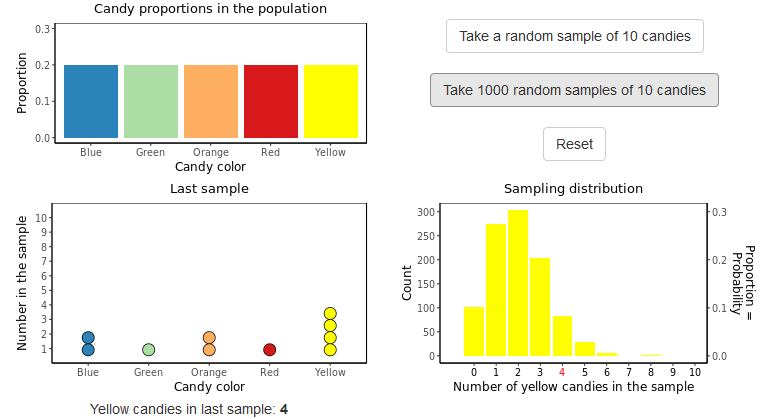
\includegraphics[width=420px]{GentleIntro_files/figure-latex/sampling-distribution-summary1-1} }\caption{A discrete sampling distribution.}\label{fig:sampling-distribution-summary1}
\end{figure}

\begin{enumerate}
\def\labelenumi{\arabic{enumi}.}
\tightlist
\item
  Figure \ref{fig:sampling-distribution-summary1} shows a simulated
  population distribution. What would be the real-world population?
\end{enumerate}

\begin{Shaded}
\begin{Highlighting}[]
\OperatorTok{*}\StringTok{ }\NormalTok{If we would really sample candies, the population could be a candy factory}\StringTok{'s}
\StringTok{stock of candies or the factory'}\NormalTok{s machine producing the candies from which we}
\NormalTok{sample.}
\end{Highlighting}
\end{Shaded}

\begin{enumerate}
\def\labelenumi{\arabic{enumi}.}
\setcounter{enumi}{1}
\tightlist
\item
  Use the button in Figure \ref{fig:sampling-distribution-summary1} to
  draw one random sample of ten candies from the population. What do the
  numbers on the horizontal axis of the bottom histogram represent? What
  is the statistical name of the variable \emph{Number of yellow
  candies}? What is the unit of analysis for this characteristic?
\end{enumerate}

\begin{Shaded}
\begin{Highlighting}[]
\OperatorTok{*}\StringTok{ }\NormalTok{The numbers on the horizontal axis of the bottom histogram represent the}
\NormalTok{number of yellow candies }\ControlFlowTok{in}\NormalTok{ the }\KeywordTok{sample}\NormalTok{(s) that we have drawn. The variable }\ControlFlowTok{for}
\NormalTok{which these numbers are values is called a sample statistic.}
\OperatorTok{*}\StringTok{ }\NormalTok{A sample statistic is a characteristic of a sample; we have a sample}
\NormalTok{statistic score }\ControlFlowTok{for}\NormalTok{ each sample that we draw. The sample, then, is the unit of}
\NormalTok{analysis or case }\ControlFlowTok{for}\NormalTok{ this variable and this histogram.}
\end{Highlighting}
\end{Shaded}

\begin{enumerate}
\def\labelenumi{\arabic{enumi}.}
\setcounter{enumi}{2}
\tightlist
\item
  Which values can the sample characteristic take here and what is the
  statistical name for this set of values?
\end{enumerate}

\begin{Shaded}
\begin{Highlighting}[]
\OperatorTok{*}\StringTok{ }\NormalTok{The sample characteristic is the number of yellow candies }\ControlFlowTok{in}\NormalTok{ our sample.}
\NormalTok{Because our sample contains ten candies, this number can vary between zero and}
\NormalTok{ten. This range of values is called the sampling space.}
\end{Highlighting}
\end{Shaded}

\begin{enumerate}
\def\labelenumi{\arabic{enumi}.}
\setcounter{enumi}{3}
\tightlist
\item
  If you would draw many samples from this population each containing
  ten candies, what is the number of yellow candies per sample that
  appears most frequently? Draw 1,000 samples to verify your answer.
\end{enumerate}

\begin{Shaded}
\begin{Highlighting}[]
\OperatorTok{*}\StringTok{ }\NormalTok{If the proportion of yellow candies is .}\DecValTok{2} \ControlFlowTok{in}\NormalTok{ the population, we expect that}
\NormalTok{this is the proportion of yellow candies that is most likely }\ControlFlowTok{in}\NormalTok{ our sample.}
\NormalTok{Therefore, samples with this proportion of yellow candies are most frequent }\ControlFlowTok{if}
\NormalTok{we draw many samples. Each sample contains ten candies, so a proportion of .}\DecValTok{2}
\NormalTok{equals two yellow candies }\ControlFlowTok{in}\NormalTok{ a sample.}
\end{Highlighting}
\end{Shaded}

\begin{enumerate}
\def\labelenumi{\arabic{enumi}.}
\setcounter{enumi}{4}
\tightlist
\item
  Is the colour distribution in each sample that you draw representative
  of the colour distribution in the stock of candies?
\end{enumerate}

\begin{Shaded}
\begin{Highlighting}[]
\OperatorTok{*}\StringTok{ }\NormalTok{No. }
\OperatorTok{*}\StringTok{ }\NormalTok{Let us assume that all colours have equal shares }\ControlFlowTok{in}\NormalTok{ the candy population,}
\NormalTok{like the example }\ControlFlowTok{in}\NormalTok{ the Figure. A sample is representative of the population}
\NormalTok{with respect to candy colour }\ControlFlowTok{if}\NormalTok{ the colors have equal shares also }\ControlFlowTok{in}\NormalTok{ the}
\NormalTok{sample. This is the only sample that is }\KeywordTok{representative}\NormalTok{ (of the candy}
\NormalTok{population) with respect to candy colours. But most of the samples that we}
\NormalTok{draw have an unequal distribution of colours. These samples are not}
\NormalTok{representative of the population.}
\end{Highlighting}
\end{Shaded}

\begin{enumerate}
\def\labelenumi{\arabic{enumi}.}
\setcounter{enumi}{5}
\tightlist
\item
  Why, do you think, is the sample characteristic (sample statistic)
  called a \emph{random variable}?
\end{enumerate}

\begin{Shaded}
\begin{Highlighting}[]
\OperatorTok{*}\StringTok{ }\NormalTok{As we see when we draw several samples, the number of yellow candies varies}
\NormalTok{across samples. This variation arises because we draw samples at random. So}
\NormalTok{the scores of samples on the sample statistic is partly random. That is a good}
\NormalTok{reason }\ControlFlowTok{for}\NormalTok{ calling it a random variable.}
\end{Highlighting}
\end{Shaded}

\begin{figure}[H]
\href{http://82.196.4.233:3838/apps/p-values/}{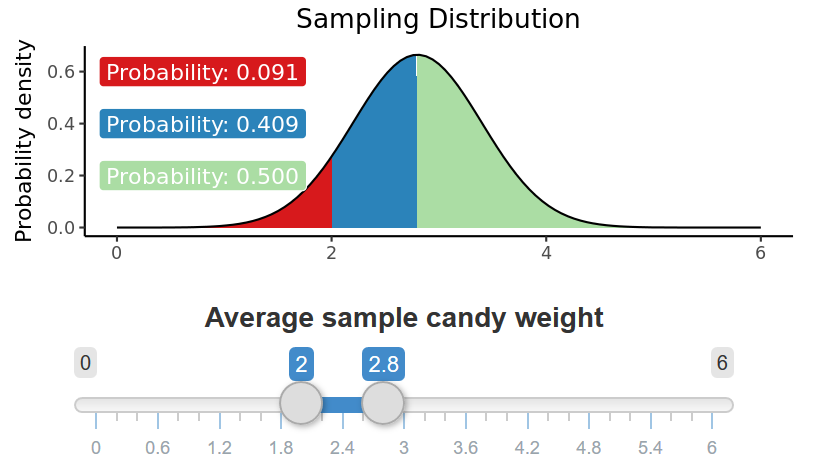
\includegraphics[width=420px]{GentleIntro_files/figure-latex/sampling-distribution-summary2-1} }\caption{A continuous sampling distribution.}\label{fig:sampling-distribution-summary2}
\end{figure}

\begin{enumerate}
\def\labelenumi{\arabic{enumi}.}
\setcounter{enumi}{6}
\tightlist
\item
  Use your own words to explain what the sampling distribution in Figure
  \ref{fig:sampling-distribution-summary2} represents.
\end{enumerate}

\begin{Shaded}
\begin{Highlighting}[]
\OperatorTok{*}\StringTok{ }\NormalTok{The sampling distribution }\ControlFlowTok{in}\NormalTok{ this figure shows average candy weights }\ControlFlowTok{for}\NormalTok{ all}
\NormalTok{possible or a very large number of random samples drawn from a population of}
\NormalTok{candies, }\ControlFlowTok{for}\NormalTok{ example, a factory}\StringTok{'s stock.}
\end{Highlighting}
\end{Shaded}

\begin{enumerate}
\def\labelenumi{\arabic{enumi}.}
\setcounter{enumi}{7}
\tightlist
\item
  What do you think is the average weight of all candies in the
  population? Justify your answer using the concepts \emph{expected
  value} and \emph{unbiased estimator}.
\end{enumerate}

\begin{Shaded}
\begin{Highlighting}[]
\OperatorTok{*}\StringTok{ }\NormalTok{The population is not depicted here, so we must infer average candy weight}
\ControlFlowTok{in}\NormalTok{ the population from the sampling distribution. If the sample statistic is}
\NormalTok{an unbiased estimator of the population }\KeywordTok{statistic}\NormalTok{ (this is the case }\ControlFlowTok{for}\NormalTok{ a}
\NormalTok{sample mean), the average of the sampling }\KeywordTok{distribution}\NormalTok{ (this is called the}
\NormalTok{expected value) is equal to the population statistic.}
\OperatorTok{*}\StringTok{ }\NormalTok{In the current example, the average of the sampling distribution of average}
\NormalTok{sample bag candy weights is equal to average candy weight }\ControlFlowTok{in}\NormalTok{ the population.}
\OperatorTok{*}\StringTok{ }\NormalTok{The sampling distribution depicted here is symmetrical, so the average}
\NormalTok{equals the median value, so half of the observed average sample candy weights}
\NormalTok{are below this value and the other half is above this value.}
\OperatorTok{*}\StringTok{ }\NormalTok{If one of the slider handles demarcates half of the probability from the}
\NormalTok{other half, this handle indicates the average of the sampling distribution. In}
\NormalTok{this example, the average is }\FloatTok{2.8}\NormalTok{ (grams).}
\end{Highlighting}
\end{Shaded}

\begin{enumerate}
\def\labelenumi{\arabic{enumi}.}
\setcounter{enumi}{8}
\tightlist
\item
  Use the sliders to find the probability of drawing a sample with
  average candy weight between 2.0 and 2.9 grams.
\end{enumerate}

\begin{Shaded}
\begin{Highlighting}[]
\OperatorTok{*}\StringTok{ }\NormalTok{If you set the left}\OperatorTok{-}\NormalTok{hand slider handle to }\FloatTok{2.0}\NormalTok{ and the right}\OperatorTok{-}\NormalTok{hand handle to}
\FloatTok{2.9}\NormalTok{, the blue area represents the probability of drawing a sample with average}
\NormalTok{candy weight between }\FloatTok{2.0}\NormalTok{ and }\FloatTok{2.9}\NormalTok{ grams. The value of the probability is}
\NormalTok{depicted }\ControlFlowTok{in}\NormalTok{ the blue box within the graph. It is .}\DecValTok{475}\NormalTok{.}
\end{Highlighting}
\end{Shaded}

\begin{enumerate}
\def\labelenumi{\arabic{enumi}.}
\setcounter{enumi}{9}
\tightlist
\item
  What, do you expect, is the probability of drawing a sample with
  average candy weight of exactly 2.9 grams? Use the sliders to check
  your expectation.
\end{enumerate}

\begin{Shaded}
\begin{Highlighting}[]
\OperatorTok{*}\StringTok{ }\NormalTok{This probability }\KeywordTok{is}\NormalTok{ (virtually) zero. If we would measure weight with very}
\NormalTok{high precision, no candy bag would have average candy weigth of exactly }\FloatTok{2.9}
\NormalTok{grams, that is, }\FloatTok{2.90000000000000000000000000}\NormalTok{(and so on) grams.}
\end{Highlighting}
\end{Shaded}

\begin{enumerate}
\def\labelenumi{\arabic{enumi}.}
\setcounter{enumi}{10}
\tightlist
\item
  Why is this graph an example of a continuous probability distribution?
\end{enumerate}

\begin{Shaded}
\begin{Highlighting}[]
\OperatorTok{*}\StringTok{ }\NormalTok{See the answer to Exercise }\DecValTok{10}\NormalTok{. A variable is continuous }\ControlFlowTok{if}\NormalTok{ we can, }\ControlFlowTok{in}
\NormalTok{principle, always find a new value between two values. This applies to weight}
\NormalTok{as a variable, because we can }\ControlFlowTok{in}\NormalTok{ principle always use more decimal places }\ControlFlowTok{in}
\NormalTok{our measurement to find a weight that is between two other weights. For}
\NormalTok{example, between }\FloatTok{2.90000}\NormalTok{ and }\FloatTok{2.90001}\NormalTok{ we can think of the weight }\FloatTok{2.900005}\NormalTok{.}
\OperatorTok{*}\StringTok{ }\NormalTok{If the sample statistic is a continuous variable, such as average candy}
\NormalTok{weight }\ControlFlowTok{in}\NormalTok{ the sample, the probability distribution }\ControlFlowTok{for}\NormalTok{ this sample statistic}
\NormalTok{is continuous.}
\end{Highlighting}
\end{Shaded}

\begin{enumerate}
\def\labelenumi{\arabic{enumi}.}
\setcounter{enumi}{11}
\tightlist
\item
  Why is the vertical axis labelled with ``Probability density'' instead
  of ``Probability''?
\end{enumerate}

\begin{Shaded}
\begin{Highlighting}[]
\OperatorTok{*}\StringTok{ }\NormalTok{It makes no sense to speak of the }\KeywordTok{probability}\NormalTok{ (vertical axis) that average}
\NormalTok{candy weight }\ControlFlowTok{in}\NormalTok{ a }\KeywordTok{sample}\NormalTok{ (horizontal axis) has one particular value. Because}
\NormalTok{average weight is a continuous }\KeywordTok{variable}\NormalTok{ (see Exercise }\DecValTok{11}\NormalTok{), the probability of}
\NormalTok{one particular outcome value }\KeywordTok{is}\NormalTok{ (virtually) }\KeywordTok{zero}\NormalTok{ (see Exercise }\DecValTok{10}\NormalTok{). If we would}
\NormalTok{draw the probabilities on the vertical axis, we would have a flat }\KeywordTok{line}\NormalTok{ (at}
\NormalTok{zero) instead of a curve.}
\OperatorTok{*}\StringTok{ }\NormalTok{Instead of probabilities of single outcome values, we are interested }\ControlFlowTok{in}
\NormalTok{probabilities of ranges or intervals of outcome values }\ControlFlowTok{if}\NormalTok{ we have a continuous}
\NormalTok{random variable. For example, the probability of a sample with average candy}
\NormalTok{weight between }\FloatTok{2.8}\NormalTok{ and }\FloatTok{2.9}\NormalTok{ grams. The probability of a range of outcome values}
\NormalTok{is depicted as a surface below a probability density function. This is what}
\NormalTok{our graph of a continuous sampling distribution shows, so the vertical axis is}
\NormalTok{labelled }\StringTok{'probability density'}\NormalTok{ instead of }\StringTok{'probability'}\NormalTok{.}
\end{Highlighting}
\end{Shaded}

\section{Take-Home Points}\label{take-home-points}

\begin{itemize}
\item
  Values of a sample statistic vary across random samples from the same
  population. But some values are more probable than other values.
\item
  The sampling distribution of a sample statistic tells us the
  probability of drawing a sample with a particular value of the sample
  statistic or a particular minimum/maximum value.
\item
  If a sample statistic is an unbiased estimator of a parameter, the
  parameter value is the average of the sampling distribution, which is
  called the expected value or expectation.
\item
  For discrete sample statistics, the sampling distribution tells us the
  probability of individual sample outcomes. For continuous sample
  statistics, it tells us the p value: the probability of drawing a
  sample with an outcome that is at least or at most a particular value.
\end{itemize}

\chapter{Probability Models: How Do I Get a Sampling
Distribution?}\label{probmodels}

\begin{quote}
Key concepts: bootstrapping/bootstrap sample, sampling with replacement,
exact approach, approximation with a theoretical probability
distribution, binomial distribution, (standard) normal distribution,
(Student) \emph{t} distribution, \emph{F} distribution, chi-squared
distribution, condition checks for theoretical probability
distributions, sample size, equal population variances, expected values,
independent samples, dependent/paired samples.
\end{quote}

\subsection*{Summary}\label{summary-1}
\addcontentsline{toc}{subsection}{Summary}

\begin{quote}
How do we get a sampling distribution without drawing many samples
ourselves?
\end{quote}

In the previous chapter, we drew a large number of samples from a
population to obtain the sampling distribution of a sample statistic,
for instance, the proportion of yellow candies or average candy weight
in the sample. The procedure is quite simple: Draw a sample, calculate
the desired sample statistic, add the sample statistic value to the
sampling distribution, and repeat this thousands of times.

Although this procedure is simple, it is not practical. In a research
project, we would have to draw thousands of samples and administer a
survey to each sample or collect data on the sample in some other way.
This requires too much time and money to be of any practical value. So
how do we create a sampling distribution, if we only collect data for a
single sample? This chapter presents three ways of doing this:
bootstrapping, exact approaches, and theoretical approximations.

\section{The Bootstrap Approximation of the Sampling
Distribution}\label{boot-approx}

The first way to obtain a sampling distribution is still based on the
idea of drawing a large number of samples. However, we only draw one
sample from the population for which we collect data. As a next step, we
draw a large number of samples from our initial sample. The samples
drawn in the second step are called \emph{bootstrap samples}. The
technique was developed by Bradley Efron
(\protect\hyperlink{ref-RefWorks:3956}{1979};
\protect\hyperlink{ref-RefWorks:3957}{1987}). For each bootstrap sample,
we calculate the sample statistic of interest and we collect these as
our sampling distribution. We usually want about 5,000 bootstrap samples
for our sampling distribution.

\begin{figure}[H]
\href{http://82.196.4.233:3838/apps/bootstrapping/}{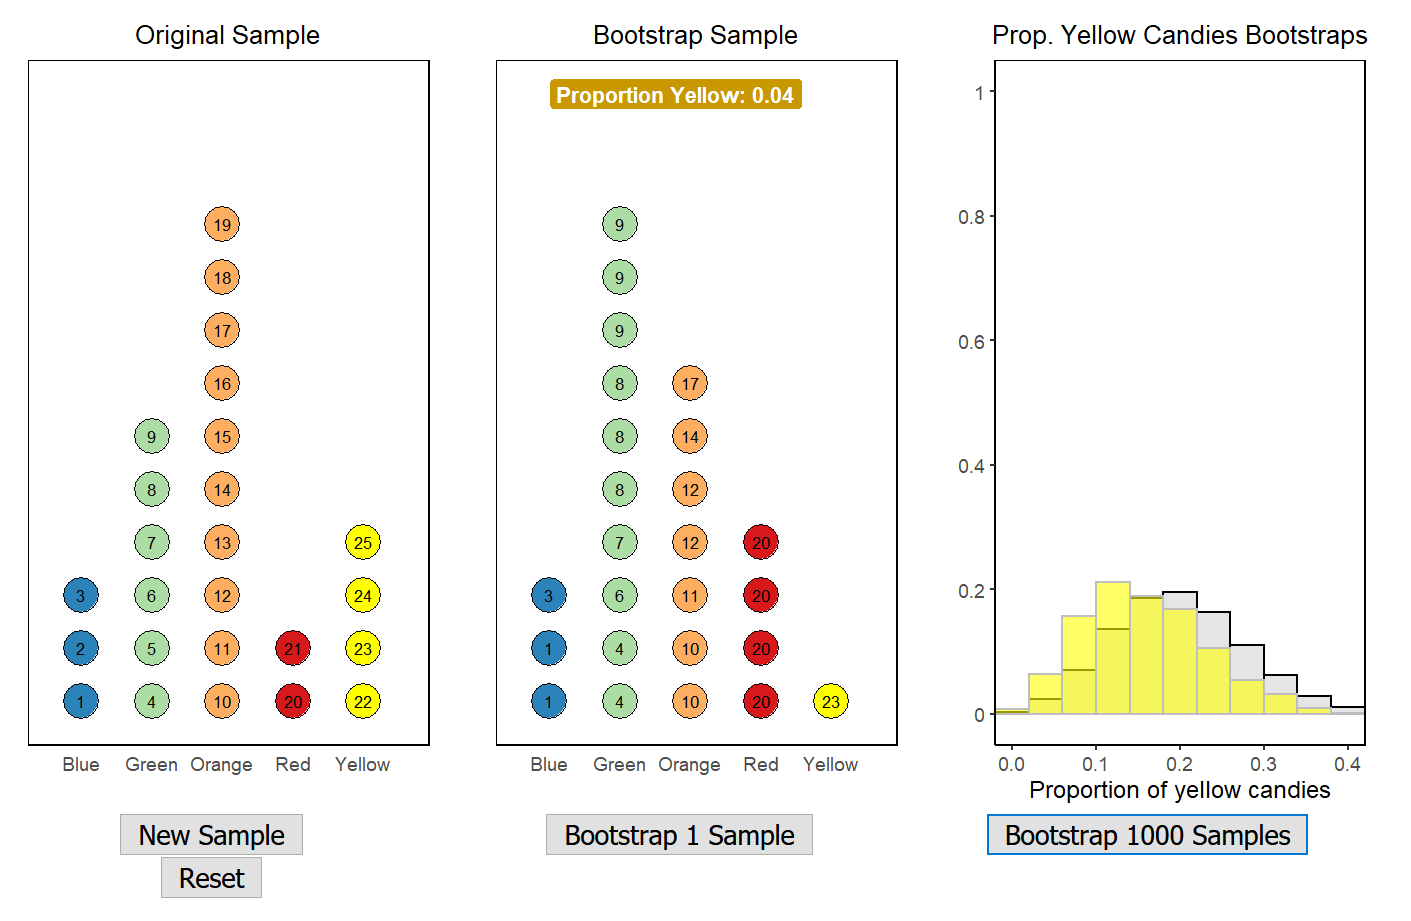
\includegraphics[width=420px]{GentleIntro_files/figure-latex/bootstrapping-1} }\caption{How do we create a sampling distribution with bootstrapping?}\label{fig:bootstrapping}
\end{figure}

In Figure \ref{fig:bootstrapping}, an initial sample has been drawn from
a population containing five candy colours in equal proportions.

\begin{enumerate}
\def\labelenumi{\arabic{enumi}.}
\tightlist
\item
  How large is a bootstrap sample in Figure \ref{fig:bootstrapping}? Use
  the \emph{Bootstrap one sample} button.
\end{enumerate}

\begin{Shaded}
\begin{Highlighting}[]
\OperatorTok{*}\StringTok{ }\NormalTok{A bootstrap sample must be just as large as the initial sample. In this}
\NormalTok{example, the initial sample contains fifty candies, so the bootstrap sample}
\NormalTok{must also contain fifty candies.}
\OperatorTok{*}\StringTok{ }\NormalTok{As we will find out later, the size of a sample is very important to the}
\NormalTok{sampling distribution, so we must draw bootstrap samples with exactly the same}
\NormalTok{number of observations as the initial sample.}
\end{Highlighting}
\end{Shaded}

\begin{enumerate}
\def\labelenumi{\arabic{enumi}.}
\setcounter{enumi}{1}
\tightlist
\item
  What element in Figure \ref{fig:bootstrapping} represents the true
  sampling distribution in this example? If in doubt, see Figure
  \ref{fig:probability-distribution}.
\end{enumerate}

\begin{Shaded}
\begin{Highlighting}[]
\OperatorTok{*}\StringTok{ }\NormalTok{The sampling distribution of a sample proportion is an exact distribution}
\NormalTok{(named binomial distribution)}\OperatorTok{:}\StringTok{ }\NormalTok{the probabilities of every number or proportion}
\NormalTok{of yellow candies }\ControlFlowTok{in}\NormalTok{ the sample can be calculated. The results are displayed}
\NormalTok{as a grey histogram at the bottom of the figure.}
\end{Highlighting}
\end{Shaded}

\begin{enumerate}
\def\labelenumi{\arabic{enumi}.}
\setcounter{enumi}{2}
\tightlist
\item
  Does the bootstrap sampling distribution resemble the true sampling
  distribution? Use the ``Bootstrap 1000 samples'' button and justify
  your answer.
\end{enumerate}

\begin{Shaded}
\begin{Highlighting}[]
\OperatorTok{*}\StringTok{ }\NormalTok{The proportion of yellow candies }\ControlFlowTok{in} \KeywordTok{the}\NormalTok{ (first) initial sample is .}\DecValTok{2}\NormalTok{, that}
\NormalTok{is, ten out of fifty candies }\ControlFlowTok{in}\NormalTok{ the sample are yellow.}
\OperatorTok{*}\StringTok{ }\NormalTok{The initial sample is representative of the population with respect to candy}
\NormalTok{colour, because the proportion of yellow candies }\ControlFlowTok{in}\NormalTok{ the population is also .}\DecValTok{2}\NormalTok{.}
\OperatorTok{*}\StringTok{ }\NormalTok{As a result, the bootstrapped sampling }\KeywordTok{distribution}\NormalTok{ (yellow histogram) is}
\NormalTok{very similar to the }\KeywordTok{true}\NormalTok{ (exact) sampling }\KeywordTok{distribution}\NormalTok{ (grey histogram).}
\end{Highlighting}
\end{Shaded}

\begin{enumerate}
\def\labelenumi{\arabic{enumi}.}
\setcounter{enumi}{3}
\tightlist
\item
  Draw a new initial sample. This sample is probably less representative
  of the distribution of candy colour in the population. What happens to
  the bootstrap samples and the bootstrap sampling distribution?
\end{enumerate}

\begin{Shaded}
\begin{Highlighting}[]
\OperatorTok{*}\StringTok{ }\NormalTok{If the proportion of yellow candies }\ControlFlowTok{in}\NormalTok{ the original sample is}
\NormalTok{close to .}\DecValTok{2}\NormalTok{, that is, ten out of fifty candies }\ControlFlowTok{in}\NormalTok{ the sample are yellow, the}
\NormalTok{bootstrapped sampling }\KeywordTok{distribution}\NormalTok{ (yellow histogram) is very similar to the}
\KeywordTok{true}\NormalTok{ (exact) sampling }\KeywordTok{distribution}\NormalTok{ (grey histogram).}
\OperatorTok{*}\StringTok{ }\NormalTok{If there are considerably less or more than ten yellow candies }\ControlFlowTok{in}\NormalTok{ the sample,}
\NormalTok{however, the bootstrapped sampling distribution is quite different from the}
\NormalTok{true sampling distribution. Especially the }\KeywordTok{mean}\NormalTok{ (horizontal location) of the}
\NormalTok{bootstrapped sampling distribution is different. The shape of the distribution}
\NormalTok{may still be nearly the same.}
\OperatorTok{*}\StringTok{ }\NormalTok{Note that the true sampling distribution, represented by the grey histogram,}
\NormalTok{remains the same because the proportion of yellow candies }\ControlFlowTok{in}\NormalTok{ the population}
\NormalTok{remains the same, namely }\DecValTok{20}\NormalTok{ per cent.}
\end{Highlighting}
\end{Shaded}

\begin{center}\rule{0.5\linewidth}{\linethickness}\end{center}

The \emph{bootstrap} concept refers to the story in which Baron von
Münchhausen saves himself by pulling himself and his horse by his
bootstraps (or hair) out of a swamp. In a similar miraculous way, the
bootstrap samples resemble the sampling distribution even though they
are drawn from a sample instead of the population. This miracle requires
some explanation and it need not work always, as we will discuss in the
remainder of this section.

\begin{figure}[H]
\centering
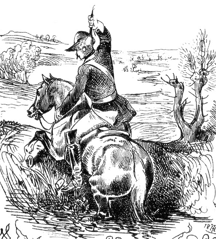
\includegraphics{figures/Munchhausen.png}
\caption{Baron von Münchhausen pulls himself and his horse out of a
swamp.}
\end{figure}

\begin{center}\rule{0.5\linewidth}{\linethickness}\end{center}

\subsection{Sampling with and without
replacement}\label{sampling-with-and-without-replacement}

As we will see in Chapter \ref{param-estim}, for example Section
\ref{precisionsesamplesize}, the size of a sample is very important to
the shape of the sampling distribution. The sampling distribution of
samples with twenty cases can be very different from the sampling
distribution of samples with fourty cases. To construct a sampling
distribution from bootstrap samples, the bootstrap samples must be
exactly as large as the original sample.

How can we draw many different bootstrap samples from the original
sample if each bootstrap sample must contain the same number of cases as
the original sample?

\begin{figure}[H]
\centering
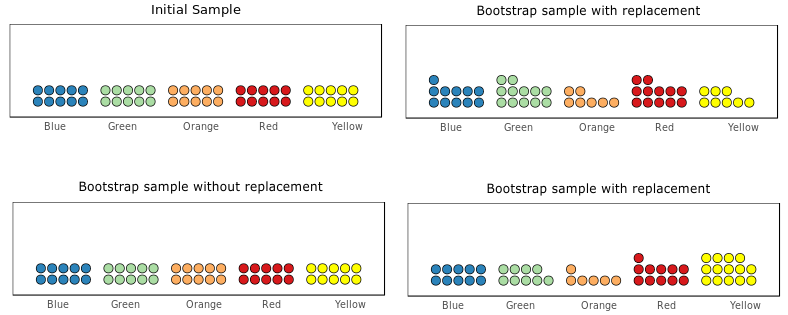
\includegraphics{figures/replacement.png}
\caption{\label{fig:replacement}Sampling with and without replacement.}
\end{figure}

\begin{enumerate}
\def\labelenumi{\arabic{enumi}.}
\tightlist
\item
  What are the differences between sampling with and without replacement
  (Figure \ref{fig:replacement})?
\end{enumerate}

\begin{Shaded}
\begin{Highlighting}[]
\OperatorTok{*}\StringTok{ }\NormalTok{If we draw a sample without replacement from our initial sample of the same}
\NormalTok{size as the initial sample, the new sample must contain all observations from}
\NormalTok{the initial sample. As a result, the new sample is identical to the initial}
\NormalTok{sample. All samples that we draw are identical.}
\OperatorTok{*}\StringTok{ }\NormalTok{Drawing with replacement, an observation can be drawn more than once. This}
\NormalTok{must have occurred }\ControlFlowTok{for}\NormalTok{ at least one red candy }\ControlFlowTok{in}\NormalTok{ the two examples of bootstrap}
\NormalTok{samples with replacement }\ControlFlowTok{in}\NormalTok{ the figure. Otherwise, we could never have more red}
\KeywordTok{candies}\NormalTok{ (twelve or eleven) }\ControlFlowTok{in}\NormalTok{ the bootstrap sample than }\ControlFlowTok{in}\NormalTok{ the initial sample}
\NormalTok{(ten red candies).}
\end{Highlighting}
\end{Shaded}

If we allow every case in the original sample to be sampled only once,
each bootstrap sample contains all cases of the original sample, so it
is an exact copy of the original sample. Thus, we cannot create
different bootstrap samples.

By the way, we often use the type of sampling described above, which is
called \emph{sampling without replacement}. If a person is (randomly)
chosen for our sample, we do not put this person back into the
population so she or he can be chosen again. We want our respondents to
fill out our questionnaire only once or participate in our experiment
only once.

If we do allow the same person to be chosen more than once, we sample
\emph{with replacement}. The same person can occur more than once in a
sample. Bootstrap samples are sampled with replacement from the original
sample, so one bootstrap sample may differ from another. Some cases in
the original sample may not be sampled for a bootstrap sample while
other cases are sampled several times. You probably have noticed this in
Figure \ref{fig:replacement}. Sampling with replacement allows us to
obtain different bootstrap samples from the original sample, and still
have bootstrap samples of the same size as the original sample.

\subsection{Calculating probabilities with
replacement}\label{calculating-probabilities-with-replacement}

You may wonder whether it is OK to sample with replacement when we are
bootstrapping. The short answer is: Yes it is. We usually calculate
probabilities as if we sampled with replacement. Suppose we want to
calculate the probability of picking two yellow candies from a
population in which 20\% of the candies are yellow. The probability of
picking two yellow candies is then calculated as .200 times .200, that
is, .040: twice the probability of drawing a yellow candy.

In this calculation, we assume that the probability to draw a yellow
candy remains the same while we are sampling. This assumption is very
convenient because it simplifies the calculation of probabilities. The
probability of sampling the first yellow candy is assumed to be .200 and
for the second yellow candy as well. We act as if the proportion of
yellow candies in the population remains the same, namely 20 per cent,
after we have sampled the first yellow candy. This can only be true if
the yellow candy that we have sampled from is immediately replaced by a
new yellow candy the population. Otherwise, the proportion of yellow
candies in the population would decrease when we sample the first yellow
candy. The probability of sampling a second yellow candy would be
slightly lower than .200.

\subsection{Calculating probabilities without
replacement}\label{calculating-probabilities-without-replacement}

In practice, however, we never want the same respondent to participate
twice in our research because this would not yield new information. In
actual research, then, we sample \emph{without} replacement. A
respondent does not risk being sampled more than once.

How about calculating probabilities if we sample without replacement? If
we do not put the sampled yellow candy back in the population, the
number of yellow candies in the population is reduced by one after we
have drawn the first yellow candy. The probability of drawing a second
yellow candy should then be less than 20\%.

If the population is large, the decrease in the probability is too small
to be in any way relevant. For instance, if we have a population of one
million candies and 20\% is yellow, the probability of drawing the first
yellow candy is 200,000 / 1,000,000 = .200. The probability of drawing
the second yellow candy would be 199,999 / 999,999 = 0.1999992. The
difference between the two probabilities (0,0000008) is negligible.

As you can see, calculating probabilities becomes complicated if we
sample without replacement because each new draw has a new probability
for drawing a yellow candy. But we can ignore the complications if the
population is much larger than the sample because the probabilities
hardly differ from the simple probabilities that we have if we sample
with replacement.

In an empirical research project, then, we always sample respondents
(and so on) \emph{without} replacement but our statistical software
calculates probabilities as if we sampled \emph{with} replacement. This
is perfectly fine as long as the population is much larger than the
sample. If the sample contains a large share of the population, however,
we should not trust the probabilities that our software reports.

\subsection{Limitations to
bootstrapping}\label{limitations-to-bootstrapping}

Does the bootstrapped sampling distribution always reflect the true
sampling distribution?

\begin{figure}[H]
\href{http://82.196.4.233:3838/apps/bootstrap-lim/}{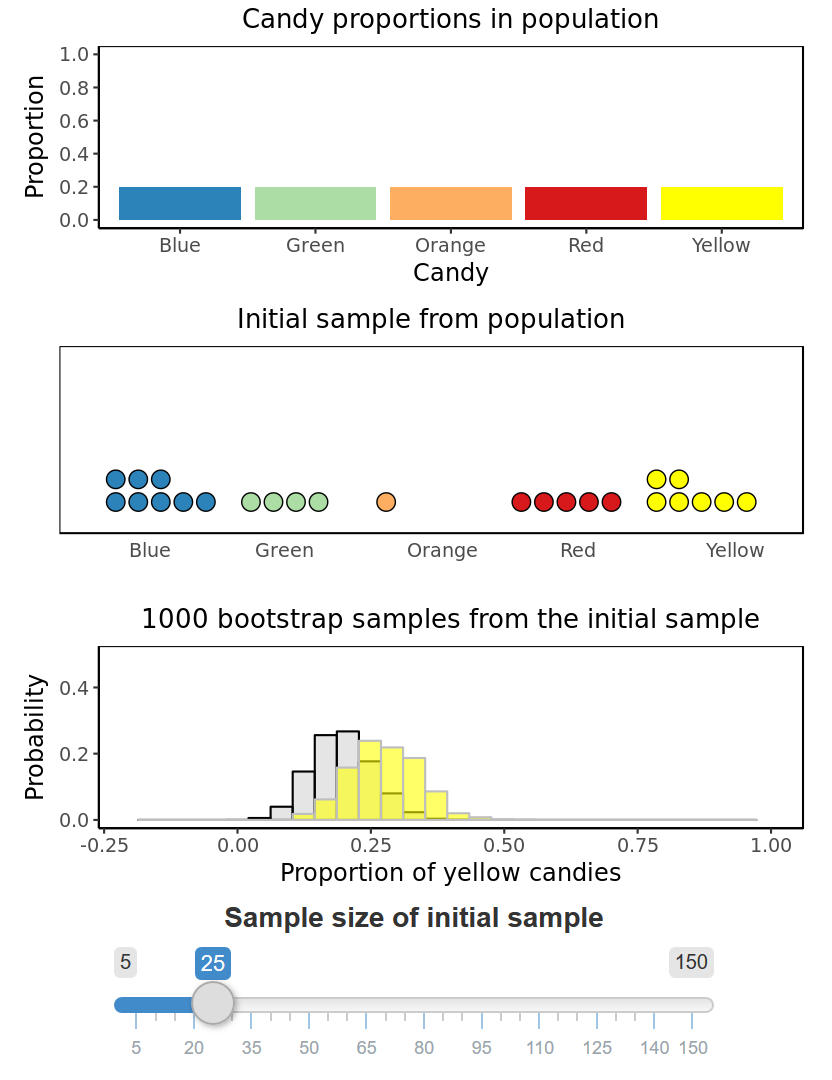
\includegraphics[width=420px]{GentleIntro_files/figure-latex/bootstrap-lim-1} }\caption{How is bootstrapping influenced by sample size? In the population, twenty per cent of the candies are yellow.}\label{fig:bootstrap-lim}
\end{figure}

\begin{enumerate}
\def\labelenumi{\arabic{enumi}.}
\tightlist
\item
  When does the bootstrap sampling distribution (yellow histogram)
  reflect the true sampling distribution (grey histogram) better: at
  small or large sample sizes? Play with sample size in Figure
  \ref{fig:bootstrap-lim} to check your answer.
\end{enumerate}

\begin{Shaded}
\begin{Highlighting}[]
\OperatorTok{*}\StringTok{ }\NormalTok{If you change sample size repeatedly between }\DecValTok{15}\NormalTok{ and }\DecValTok{45}\NormalTok{, you will see that}
\NormalTok{the bootstrapped sampling }\KeywordTok{distribution}\NormalTok{ (yellow histogram) jumps around the}
\NormalTok{true sampling }\KeywordTok{distribution}\NormalTok{ (grey histogram).}
\OperatorTok{*}\StringTok{ }\NormalTok{For relatively small sample sizes, the bootstrapped sampling distribution is}
\NormalTok{often quite different from the true sampling distribution.}
\OperatorTok{*}\StringTok{ }\NormalTok{At larger sample sizes, say between }\DecValTok{120}\NormalTok{ and }\DecValTok{150}\NormalTok{, the bootstrapped sampling}
\NormalTok{distribution overlaps the true sampling distribution much more frequently. So}
\ControlFlowTok{for}\NormalTok{ larger samples, we can trust the bootstrapped sampling distribution more.}
\NormalTok{But even then, it can sometimes be quite off the mark.}
\end{Highlighting}
\end{Shaded}

\begin{enumerate}
\def\labelenumi{\arabic{enumi}.}
\setcounter{enumi}{1}
\tightlist
\item
  How does sample size relate to representativeness of the sample in
  terms of the proportion of yellow candies? Note that twenty per cent
  of the candies in the population are yellow.
\end{enumerate}

\begin{Shaded}
\begin{Highlighting}[]
\OperatorTok{*}\StringTok{ }\NormalTok{The proportion of yellow candies }\ControlFlowTok{in}\NormalTok{ larger samples is more often close to}
\NormalTok{the proportion }\ControlFlowTok{in}\NormalTok{ the population}\OperatorTok{:}\StringTok{ }\FloatTok{0.2}\NormalTok{. This is the reason that the}
\NormalTok{bootstrapped sampling distribution usually resembles the true sampling}
\NormalTok{distribution.}
\end{Highlighting}
\end{Shaded}

\begin{enumerate}
\def\labelenumi{\arabic{enumi}.}
\setcounter{enumi}{2}
\tightlist
\item
  If you use a very small sample size, it may happen that there is no
  yellow histogram in the bottom graph. What is the matter if that
  happens?
\end{enumerate}

\begin{Shaded}
\begin{Highlighting}[]
\OperatorTok{*}\StringTok{ }\NormalTok{If we draw an initial sample without any yellow candies, none of the}
\NormalTok{bootstrap samples can include yellow candies. As a result, the count of}
\NormalTok{samples with yellow candies is always zero.}
\OperatorTok{*}\StringTok{ }\NormalTok{The smaller the initial sample, the greater the chance of having a sample}
\NormalTok{without yellow candies.}
\end{Highlighting}
\end{Shaded}

We can create a sampling distribution by sampling from our original
sample with replacement. It is hardly a miracle that we obtain different
samples with different sample statistics if we sample with replacement.
Much more miraculous, however, is that this bootstrap distribution
resembles the true sampling distribution that we would get if we draw
lots of samples directly from the population.

Does this miracle always happen? No. First, the original sample that we
have drawn from the population must not be too small. We cannot draw
many different samples from a small sample. For this reason, the
bootstrap distribution cannot resemble the true sampling distribution in
the case of a small original sample.

Second, the original sample must be more or less representative of the
population. The variables of interest in the sample should be
distributed more or less the same as in the population. If this is not
the case, the sampling distribution may be biased, giving a distorted
view of the true sampling distribution.

A sample is more likely to be representative of the population if the
sample is drawn in a truly random fashion and if the sample is larger.
But we can never be sure. There always is a chance that we have drawn a
sample that does not reflect the population well. This is the main
limitation to the bootstrap approach to sampling distributions.

\subsection{Any sample statistic can be
bootstrapped}\label{any-sample-statistic-can-be-bootstrapped}

The big advantage of the bootstrap approach (\emph{bootstrapping}),
however, is that we can get a sampling distribution for any sample
statistic that we are interested in. Every statistic that we can
calculate for our original sample can also be calculated for each
bootstrap sample. The sampling distribution is just the collection of
the sample statistics calculated for all bootstrap samples.

Bootstrapping is more or less the only way to get a sampling
distribution for the sample median, for example, the median weight of
candies in a sample bag. We may create sampling distributions for the
wildest and weirdest sample statistics, for instance the difference
between sample mean and sample median squared. I would not know why you
would be interested in the squared difference of sample mean and median,
but there are very interesting statistics that we can only get at
through bootstrapping. A case in point is the strength of an indirect
effect in a mediation model (Chapter \ref{mediation}).

\section{Bootstrapping in SPSS}\label{boot-spss}

\subsection{Instructions}\label{instructions}

\begin{figure}[H]
\href{https://www.youtube.com/embed/6-MtiMhuuIg}{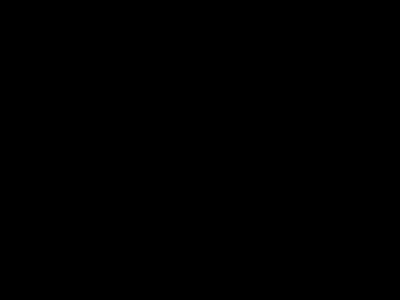
\includegraphics[width=320px]{GentleIntro_files/figure-latex/SPSSbootstrap1-1} }\caption{Bootstrapping in SPSS.}\label{fig:SPSSbootstrap1}
\end{figure}

\begin{figure}[H]
\href{https://www.youtube.com/embed/6E2LgeMtkL4}{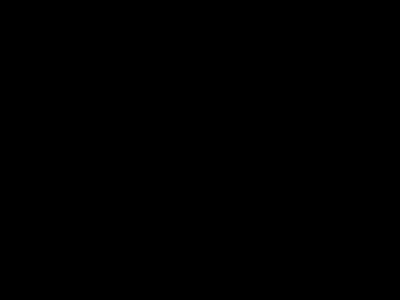
\includegraphics[width=320px]{GentleIntro_files/figure-latex/SPSSbootstrap2-1} }\caption{Interpreting bootstrap results in SPSS.}\label{fig:SPSSbootstrap2}
\end{figure}

In principle, any sample statistic can be bootstrapped. SPSS, however,
does not bootstrap all sample statistics. For example, SPSS does not
bootstrap the minimum value, maximum value or the range between minimum
and maximum value of a variable.

\subsection{Exercises}\label{exercises}

\begin{enumerate}
\def\labelenumi{\arabic{enumi}.}
\tightlist
\item
  Download the data set
  \href{http://82.196.4.233:3838/data/candies.sav}{candies.sav} and use
  SPSS to bootstrap the t test on average weight of yellow and red
  candies (the example above). The test is available in the
  \emph{Analyze\textgreater{}Compare Means} menu.
\end{enumerate}

\begin{Shaded}
\begin{Highlighting}[]
\NormalTok{SPSS syntax}\OperatorTok{:}\StringTok{  }
\StringTok{    }
\ErrorTok{*}\StringTok{ }\NormalTok{Exercise }\DecValTok{1}\OperatorTok{:}\StringTok{ }\NormalTok{Bootstrap different averages.  }
\OperatorTok{*}\StringTok{ }\NormalTok{Check data.  }
\NormalTok{FREQUENCIES VARIABLES=colour weight  }
  \OperatorTok{/}\NormalTok{ORDER=ANALYSIS.  }
\OperatorTok{*}\StringTok{ }\NormalTok{Execute independent}\OperatorTok{-}\NormalTok{samples t test with bootstrap.  }
\NormalTok{BOOTSTRAP  }
  \OperatorTok{/}\NormalTok{SAMPLING METHOD=SIMPLE  }
  \OperatorTok{/}\NormalTok{VARIABLES TARGET=weight INPUT=colour   }
  \OperatorTok{/}\NormalTok{CRITERIA CILEVEL=}\DecValTok{95}\NormalTok{ CITYPE=BCA  NSAMPLES=}\DecValTok{5000}  
  \OperatorTok{/}\NormalTok{MISSING USERMISSING=EXCLUDE.  }
\NormalTok{T}\OperatorTok{-}\NormalTok{TEST GROUPS=}\KeywordTok{colour}\NormalTok{(}\DecValTok{4} \DecValTok{5}\NormalTok{)  }
  \OperatorTok{/}\NormalTok{MISSING=ANALYSIS  }
  \OperatorTok{/}\NormalTok{VARIABLES=weight  }
  \OperatorTok{/}\NormalTok{CRITERIA=}\KeywordTok{CI}\NormalTok{(.}\DecValTok{95}\NormalTok{).  }
  
\NormalTok{Check data}\OperatorTok{:}\StringTok{  }
\StringTok{  }
\NormalTok{There are no impossible values on the two variables.    }
      
\NormalTok{Check assumptions}\OperatorTok{:}\StringTok{  }
\StringTok{  }
\NormalTok{The measurement levels of the variables are OK }\ControlFlowTok{for}\NormalTok{ a t test}\OperatorTok{:}\StringTok{ }
\NormalTok{colour is a categorical variable with two values and weight is}
\NormalTok{a numeric variable. There are no additional assumptions }\ControlFlowTok{for} 
\NormalTok{bootstrapping.}
    
\NormalTok{Interpret the results}\OperatorTok{:}\StringTok{   }
\StringTok{  }
\NormalTok{The table }\StringTok{"Bootstrap for Independent Samples Test"}\NormalTok{ contains   }
\NormalTok{the results that we are interested in.   }
  
\NormalTok{Levene s test on homegeneity of variances is not statistically  }
\NormalTok{significant, so we may assume that the population variances of  }
\NormalTok{red and yellow candy weight are equal. So we interpret the  }
\NormalTok{top row }\ControlFlowTok{in}\NormalTok{ table }\StringTok{"Bootstrap for Independent Samples Test"}\NormalTok{.  }
  
\NormalTok{The mean difference between red and yellow candy weight is  }
\FloatTok{0.05}\NormalTok{ grams. In our sample, red candies are just a little  }
\NormalTok{heavier than yellow candies.  }
  
\NormalTok{The bootstrapped }\DecValTok{95}\NormalTok{% confidence interval }\ControlFlowTok{for}\NormalTok{ this difference is }\OperatorTok{-}\FloatTok{0.11}\NormalTok{ to }\FloatTok{0.21}\NormalTok{.}
\NormalTok{With }\DecValTok{95}\NormalTok{% confidence, we can say that red candies can be on average }\FloatTok{0.11}\NormalTok{ grams}
\NormalTok{lighter than yellow candies or up to }\FloatTok{0.21}\NormalTok{ grams heavier. We cannot tell which}
\NormalTok{of the two are heavier }\ControlFlowTok{in}\NormalTok{ the population with sufficient confidence.}

\NormalTok{Note that your results can be slightly different because bootstrapping creates}
\NormalTok{random samples.}
\end{Highlighting}
\end{Shaded}

\begin{enumerate}
\def\labelenumi{\arabic{enumi}.}
\setcounter{enumi}{1}
\tightlist
\item
  Use the same data set to bootstrap the median of candy weight.
  Remember that measures of central tendency can be obtained with the
  \emph{Frequencies\textgreater{}Statistics} command in the
  \emph{Analyze\textgreater{}Descriptive Statistics} menu.
\end{enumerate}

\begin{Shaded}
\begin{Highlighting}[]
\NormalTok{SPSS syntax}\OperatorTok{:}\StringTok{  }
\StringTok{    }
\ErrorTok{*}\StringTok{ }\NormalTok{Exercise }\DecValTok{2}\OperatorTok{:}\StringTok{ }\NormalTok{Bootstrap on median candy weight.  }
\OperatorTok{*}\StringTok{ }\NormalTok{Check data.  }
\NormalTok{FREQUENCIES VARIABLES=weight  }
  \OperatorTok{/}\NormalTok{ORDER=ANALYSIS.  }
\OperatorTok{*}\StringTok{ }\NormalTok{Bootstrap the median.  }
\NormalTok{BOOTSTRAP  }
  \OperatorTok{/}\NormalTok{SAMPLING METHOD=SIMPLE  }
  \OperatorTok{/}\NormalTok{VARIABLES INPUT=weight   }
  \OperatorTok{/}\NormalTok{CRITERIA CILEVEL=}\DecValTok{95}\NormalTok{ CITYPE=BCA  NSAMPLES=}\DecValTok{5000}  
  \OperatorTok{/}\NormalTok{MISSING USERMISSING=EXCLUDE.  }
\NormalTok{FREQUENCIES VARIABLES=weight  }
  \OperatorTok{/}\NormalTok{FORMAT=NOTABLE  }
  \OperatorTok{/}\NormalTok{STATISTICS=MEDIAN  }
  \OperatorTok{/}\NormalTok{ORDER=ANALYSIS.  }
  
\NormalTok{Check data}\OperatorTok{:}\StringTok{  }
\StringTok{    }
\NormalTok{There are no impossible values on the weight variable.  }
  
\NormalTok{Check assumptions}\OperatorTok{:}\StringTok{  }
\StringTok{    }
\NormalTok{The measurement level of variable weight is OK.  }
      
\NormalTok{Interpret the results}\OperatorTok{:}\StringTok{   }
\StringTok{  }
\NormalTok{Median candy weight }\ControlFlowTok{in}\NormalTok{ the sample is }\FloatTok{2.81}\NormalTok{ gram. With   }
\DecValTok{95}\NormalTok{% confidence, we expect median candy weight to be   }
\NormalTok{between }\FloatTok{2.78}\NormalTok{ and }\FloatTok{2.92}\NormalTok{ grams }\ControlFlowTok{in}\NormalTok{ the population of all candies.  }
\NormalTok{The }\DecValTok{95}\NormalTok{% interval borders can be slightly different because}
\NormalTok{bootstrapping takes random samples.}
\end{Highlighting}
\end{Shaded}

\section{Exact Approaches to the Sampling
Distribution}\label{exact-approaches-to-the-sampling-distribution}

A second approach to constructing a sampling distribution has implicitly
been demonstrated in the preceding section on bootstrapping (Section
\ref{boot-approx}) and the section on probability distributions (Section
\ref{probdistribution}). In these sections, we calculated the true
sampling distribution of the proportion of yellow candies in a sample
from the probabilities of the colours. If we know or think we know the
proportion of yellow candies in the population, we can exactly calculate
the probability that a sample of ten candies includes one, two, three,
or ten yellow candies. See the section on discrete random variables for
details (Section \ref{discreterandomvariable}).

\begin{table}[H]

\caption{\label{tab:exact-approach}Number of heads for a toss of three coins.}
\centering
\fontsize{8}{8}\selectfont
\begin{tabular}[t]{lllr}
\hline
Outcome & Combination & Probability: Combination & Probability: Outcome\\
\hline
0 & tail-tail-tail & 1/2 * 1/2 * 1/2 = 1/8 =  .125 & 1/8 =  .125\\
1 & tail-tail-head & 1/2 * 1/2 * 1/2 = 1/8 =  .125 & \\
1 & head-tail-tail & 1/2 * 1/2 * 1/2 = 1/8 =  .125 & \\
1 & tail-head-tail & 1/2 * 1/2 * 1/2 = 1/8 =  .125 & 3/8 =  .375\\
2 & head-head-tail & 1/2 * 1/2 * 1/2 = 1/8 =  .125 & \\
2 & head-tail-head & 1/2 * 1/2 * 1/2 = 1/8 =  .125 & \\
2 & tail-head-head & 1/2 * 1/2 * 1/2 = 1/8 =  .125 & 3/8 =  .375\\
3 & head-head-head & 1/2 * 1/2 * 1/2 = 1/8 =  .125 & 1/8 =  .125\\
\hline
Total & 8 &  & 1.000\\
\hline
\end{tabular}
\end{table}

\begin{enumerate}
\def\labelenumi{\arabic{enumi}.}
\tightlist
\item
  Explain the meaning of the entries in the column \textbf{Combination}
  and how they relate to the entries in the \textbf{Outcome} column.
\end{enumerate}

\begin{Shaded}
\begin{Highlighting}[]
\OperatorTok{*}\StringTok{ }\NormalTok{The column }\StringTok{"Combination"}\NormalTok{ lists all posible outcomes }\ControlFlowTok{if}\NormalTok{ we toss three coins.}
\OperatorTok{*}\StringTok{ }\NormalTok{The sample statistic is the number of heads }\ControlFlowTok{in}\NormalTok{ a throw of three coins, which}
\NormalTok{is reported }\ControlFlowTok{in}\NormalTok{ the }\StringTok{"Outcome"}\NormalTok{ column. It simply counts the number of heads that}
\NormalTok{appear }\ControlFlowTok{in}\NormalTok{ the combination.}
\OperatorTok{*}\StringTok{ }\NormalTok{This number can range from zero to three. This is the sampling space.}
\end{Highlighting}
\end{Shaded}

\begin{enumerate}
\def\labelenumi{\arabic{enumi}.}
\setcounter{enumi}{1}
\tightlist
\item
  Explain how the combinations relate to the probabilities.
\end{enumerate}

\begin{Shaded}
\begin{Highlighting}[]
\OperatorTok{*}\StringTok{ }\NormalTok{There are eight combinations. If the coins are fair, each combination has}
\NormalTok{the same probability to appear, namely }\DecValTok{1}\OperatorTok{/}\DecValTok{8}\NormalTok{ =}\StringTok{ }\NormalTok{.}\DecValTok{125}\NormalTok{. We sum the probabilities }\ControlFlowTok{for}
\NormalTok{all combinations that have the same outcome, namely the same number of heads.}
\OperatorTok{*}\StringTok{ }\NormalTok{Thus we arrive at the probability of having no heads }\ControlFlowTok{in}\NormalTok{ a }\KeywordTok{throw}\NormalTok{ (}\DataTypeTok{p =}\NormalTok{ .}\DecValTok{125}\NormalTok{),}
\NormalTok{one }\KeywordTok{head}\NormalTok{ (}\DataTypeTok{p =}\NormalTok{ .}\DecValTok{375}\NormalTok{), and so on.}
\end{Highlighting}
\end{Shaded}

The calculated probabilities of all possible sample statistic outcomes
give us an exact approach to the sampling distribution. Note that I use
the word \emph{approach} instead of \emph{approximation} here because
the obtained sampling distribution is no longer an approximation, that
is, more or less similar to the true sampling distribution. No, it is
the true sampling distribution itself.

\subsection{Exact approaches for categorical
data}\label{exact-approaches-for-categorical-data}

An exact approach lists and counts all possible combinations. This can
only be done if we work with discrete or categorical variables. For an
unlimited number of categories, we cannot list all possible
combinations.

A proportion is based on frequencies and frequencies are discrete
(integer values), so we can use an exact approach to create a sampling
distribution for one proportion such as the proportion of yellow candies
in the example above. The exact approach uses the binomial probability
formula to calculate probabilities. Consult the internet if you want to
know this formula; we are not going to use it here.

Exact approaches are also available for the association between two
categorical (nominal or ordinal) variables in a contingency table: Do
some combinations of values for the two variables occur relatively
frequently? For example, are yellow candies more often sticky than red
candies? If candies are either sticky or not sticky and they have one
out of a limited set of colours, we have two categorical variables. We
can create an exact probability distribution for the combination of
colour and stickiness. The \emph{Fisher-exact test} is an example of an
exact approach to the sampling distribution of the association between
two categorical variables.

\subsection{Computer-intensive}\label{computer-intensive}

The exact approach can be applied to discrete variables because they
have a limited number of values. Discrete variables are usually measured
at the nominal or ordinal level. If the number of categories becomes
large, a lot of computing time can be needed to calculate the
probabilities of all possible sample statistic outcomes. Exact
approaches are said to be \emph{computer-intensive}.

It is usually wise to set a limit to the time you allow your computer to
work on an exact sampling distribution because otherwise the problem may
keep your computer occupied for hours or days.

\section{Exact Approaches in SPSS}\label{SPSS-exact}

\subsection{Instructions}\label{instructions-1}

\begin{figure}[H]
\href{https://www.youtube.com/embed/7cZKqrlofAs}{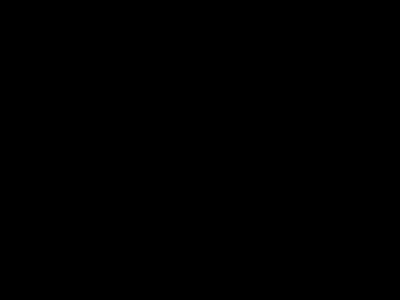
\includegraphics[width=320px]{GentleIntro_files/figure-latex/SPSSExact1-1} }\caption{Performing an exact test in SPSS.}\label{fig:SPSSExact1}
\end{figure}

\begin{figure}[H]
\href{https://www.youtube.com/embed/B-I6T4gCdsM}{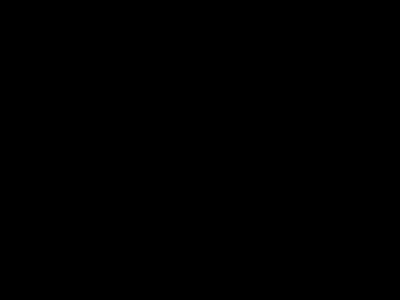
\includegraphics[width=320px]{GentleIntro_files/figure-latex/SPSSExact2-1} }\caption{Interpreting exact test results in SPSS.}\label{fig:SPSSExact2}
\end{figure}

\subsection{Exercises}\label{exercises-1}

\begin{enumerate}
\def\labelenumi{\arabic{enumi}.}
\tightlist
\item
  Download the data set
  \href{http://82.196.4.233:3838/data/candies.sav}{candies.sav} and use
  SPSS to apply a Fisher-exact test to the association between candy
  colour and candy stickiness.
\end{enumerate}

\begin{Shaded}
\begin{Highlighting}[]
\NormalTok{SPSS syntax}\OperatorTok{:}\StringTok{  }
\StringTok{  }
\ErrorTok{*}\StringTok{ }\NormalTok{Exact test on the relation between candy colour  }
\OperatorTok{*}\StringTok{ }\NormalTok{and candy stickiness.  }
\OperatorTok{*}\StringTok{ }\NormalTok{Do not forget to deselect bootstrapping }\ControlFlowTok{if}\NormalTok{ you used }
\OperatorTok{*}\StringTok{ }\NormalTok{bootstrapping }\ControlFlowTok{in}\NormalTok{ the preceding exercise.  }
\NormalTok{CROSSTABS  }
  \OperatorTok{/}\NormalTok{TABLES=colour BY sticky  }
  \OperatorTok{/}\NormalTok{FORMAT=AVALUE TABLES  }
  \OperatorTok{/}\NormalTok{STATISTICS=CHISQ PHI   }
  \OperatorTok{/}\NormalTok{CELLS=COUNT COLUMN   }
  \OperatorTok{/}\NormalTok{COUNT ROUND CELL  }
  \OperatorTok{/}\NormalTok{METHOD=EXACT }\KeywordTok{TIMER}\NormalTok{(}\DecValTok{5}\NormalTok{).  }
  
\NormalTok{Check data}\OperatorTok{:}\StringTok{  }
\StringTok{  }
\NormalTok{The contingency table does not show any impossible values }\ControlFlowTok{for}  
\NormalTok{the two categorical variables.  }
  
\NormalTok{Check assumptions}\OperatorTok{:}\StringTok{  }
\StringTok{  }
\NormalTok{There are no assumptions }\ControlFlowTok{for}\NormalTok{ a Fisher}\OperatorTok{-}\NormalTok{exact test.  }
  
\NormalTok{Interpret the results}\OperatorTok{:}\StringTok{  }
\StringTok{  }
\NormalTok{There is a strong }\KeywordTok{association}\NormalTok{ (Cramer}\StringTok{'s V = .52) between candy colour and}
\StringTok{candy stickiness, which is statistically significant, p = .010 (exact). Yellow}
\StringTok{and red candies are less often sticky than blue, green, and orange candies.}
\end{Highlighting}
\end{Shaded}

\begin{enumerate}
\def\labelenumi{\arabic{enumi}.}
\setcounter{enumi}{1}
\tightlist
\item
  With the same data, apply a Fisher-exact test to the association
  between candy colour and candy spottiness.
\end{enumerate}

\begin{Shaded}
\begin{Highlighting}[]
\NormalTok{SPSS syntax}\OperatorTok{:}\StringTok{  }
\StringTok{  }
\ErrorTok{*}\StringTok{ }\NormalTok{Exact test on the relation between candy colour  }
\OperatorTok{*}\StringTok{ }\NormalTok{and candy spottiness.  }
\OperatorTok{*}\StringTok{ }\NormalTok{Do not forget to deselect bootstrapping.  }
\NormalTok{CROSSTABS  }
  \OperatorTok{/}\NormalTok{TABLES=colour BY spotted  }
  \OperatorTok{/}\NormalTok{FORMAT=AVALUE TABLES  }
  \OperatorTok{/}\NormalTok{STATISTICS=CHISQ PHI   }
  \OperatorTok{/}\NormalTok{CELLS=COUNT COLUMN   }
  \OperatorTok{/}\NormalTok{COUNT ROUND CELL  }
  \OperatorTok{/}\NormalTok{METHOD=EXACT }\KeywordTok{TIMER}\NormalTok{(}\DecValTok{5}\NormalTok{).  }
  
\NormalTok{Check data}\OperatorTok{:}\StringTok{  }
\StringTok{  }
\NormalTok{The contingency table does not show any impossible values }\ControlFlowTok{for}  
\NormalTok{the two categorical variables.  }
  
\NormalTok{Check assumptions}\OperatorTok{:}\StringTok{  }
\StringTok{  }
\NormalTok{There are no assumptions }\ControlFlowTok{for}\NormalTok{ a Fisher}\OperatorTok{-}\NormalTok{exact test.  }
  
\NormalTok{Interpret the results}\OperatorTok{:}\StringTok{  }
\StringTok{  }
\NormalTok{There is a moderate }\KeywordTok{association}\NormalTok{ (Cramer}\StringTok{'s V = .27) between   }
\StringTok{candy colour and candy stickiness, which is   }
\StringTok{not statistically significant, p = .480 (exact) or}
\StringTok{p = .555 (exact).   }
\StringTok{Candy colour does not seem relevant to having spots.  }
\end{Highlighting}
\end{Shaded}

\section{Theoretical Approximations of the Sampling
Distribution}\label{theoretical-approximations-of-the-sampling-distribution}

Because bootstrapping and exact approaches to the sampling distribution
require quite a lot of computing power, these methods were not practical
in the not so very distant pre-computer age. In those days,
mathematicians and statisticians discovered that many sampling
distributions look a lot like known mathematical functions. For example,
the sampling distribution of the sample mean can be quite similar to the
well-known bell-shape of the \emph{normal distribution} or the closely
related \emph{(Student) t distribution}. The mathematical functions are
called \emph{theoretical probability distributions}. Most statistical
tests use a theoretical probability distribution as approximation of the
sampling distribution.

\begin{figure}[H]
\href{http://82.196.4.233:3838/apps/normal-approximation/}{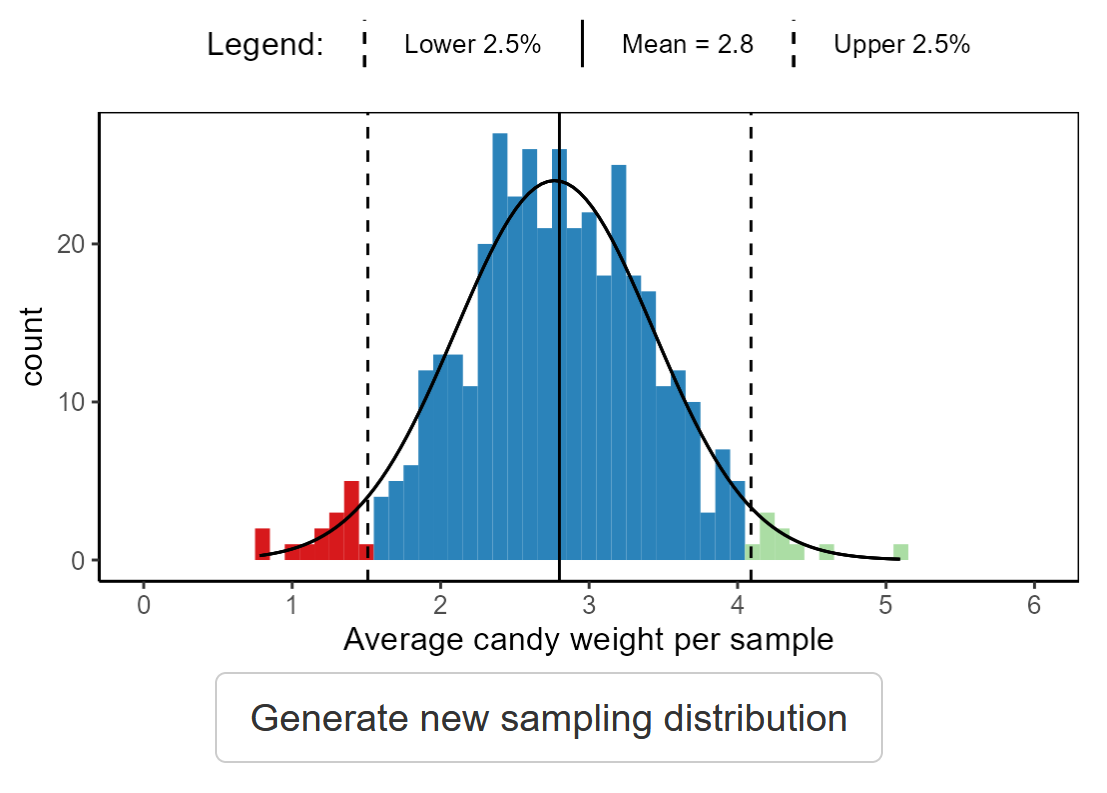
\includegraphics[width=420px]{GentleIntro_files/figure-latex/normal-approximation-1} }\caption{Normal function as theoretical approximation of a sampling distribution.}\label{fig:normal-approximation}
\end{figure}

\begin{enumerate}
\def\labelenumi{\arabic{enumi}.}
\tightlist
\item
  Figure \ref{fig:normal-approximation} displays a simulated sampling
  distribution of sample means and the normal approximation of this
  distribution (curve). Check if the normal function is a good
  approximation of the sampling distribution.
\end{enumerate}

\begin{Shaded}
\begin{Highlighting}[]
\OperatorTok{*}\StringTok{ }\NormalTok{The curve fits the histogram of observed sample means quite well.}
\NormalTok{Discrepancies are mainly due to the jagged layout of the histogram, which}
\NormalTok{results from binning the }\KeywordTok{data}\NormalTok{ (to create bars) and from the fact that the}
\NormalTok{number of samples is large but not very large.}
\OperatorTok{*}\StringTok{ }\NormalTok{For the sampling distribution of means we know that the normal }\KeywordTok{or}\NormalTok{ (Student)}
\NormalTok{t distribution represents the sampling distribution very accurately.}
\end{Highlighting}
\end{Shaded}

\begin{enumerate}
\def\labelenumi{\arabic{enumi}.}
\setcounter{enumi}{1}
\tightlist
\item
  While checking the distribution, pay special attention to the tails
  because these are used for significance tests (see Chapter
  \ref{hypothesis}). The red and green bars represent the 2.5 per cent
  samples with minimum or maximum average weight. The vertical lines
  mark the outer 2.5 per cent according to the normal function. Do the
  tail borders of the sampling distribution and normal approximation
  match?
\end{enumerate}

\begin{Shaded}
\begin{Highlighting}[]
\OperatorTok{*}\StringTok{ }\NormalTok{The borders demarcating the lowest and highest }\FloatTok{2.5}\NormalTok{% of sample means }\ControlFlowTok{in}\NormalTok{ the}
\NormalTok{theoretical probability }\KeywordTok{distribution}\NormalTok{ (the dotted lines) nicely coincide with}
\NormalTok{the border between red or green and blue bars }\ControlFlowTok{in}\NormalTok{ the histogram }\ControlFlowTok{in}\NormalTok{ most of the}
\NormalTok{sampling distributions that we generate with this app.}
\end{Highlighting}
\end{Shaded}

\begin{enumerate}
\def\labelenumi{\arabic{enumi}.}
\setcounter{enumi}{2}
\tightlist
\item
  Generate some new sampling distributions to see if the normal function
  always yields a good approximation. What changes in the distribution:
  the mean, the standard deviation, or both?
\end{enumerate}

\begin{Shaded}
\begin{Highlighting}[]
\OperatorTok{*}\StringTok{ }\NormalTok{The mean of the sampling distribution does not change. It is equal to the}
\NormalTok{population }\KeywordTok{mean}\NormalTok{ (mean candy weight }\ControlFlowTok{in}\NormalTok{ the population), so the population mean}
\NormalTok{seems not to be changed when we generate a new sampling distribution.}
\OperatorTok{*}\StringTok{ }\NormalTok{The width}\OperatorTok{/}\NormalTok{peakedness of the sampling distribution changes. This expresses}
\NormalTok{the }\KeywordTok{variation}\NormalTok{ (standard devation) }\ControlFlowTok{in}\NormalTok{ the sampling distribution. But regardless}
\NormalTok{of the amount of variation, the normal curve fits the distribution equally}
\NormalTok{well.}
\end{Highlighting}
\end{Shaded}

The normal distribution is a mathematical function linking continuous
scores, e.g., a sample statistic such as the average weight in the
sample, to p values, that is, to the probability of finding at least, or
at most, this score. Such a function is called a \emph{probability
density function} (Section \ref{cont-random-var}).

We like to use a theoretical probability distribution as an
approximation of the sampling distribution because it is convenient. The
computer can calculate probabilities from the mathematical function very
quickly. We also like theoretical probability distributions because they
usually offer plausible arguments about chance and probabilities.

\subsection{Reasons for a bell-shaped probability
distribution}\label{reasons-for-a-bell-shaped-probability-distribution}

The bell shape of the normal distribution makes sense. Our sample of
candies is just as likely to be too heavy, as it is too light, so the
sampling distribution of the sample mean should be symmetrical. A normal
distribution is symmetrical.

In addition, it is more likely that our sample bag has an average weight
that is near the true average candy weight in the population than an
average weight that is much heavier or much lighter than the true
average. Bags with on average extremely heavy or extremely light candies
may occur, but they are extremely rare (we are very lucky or very
unlucky). From these intuitions we would expect a bell shape for the
sampling distribution.

From this argumentation, we conclude that the normal distribution is a
reasonable model for the probability distribution of sample means.
Actually, it has been proven that the normal distribution exactly
represents the sampling distribution in particular cases, for instance
the sampling distribution of the mean of a very large sample.

As a model, the theoretical probability distribution may actually give a
better approximation of the sampling distribution than a sampling
distribution created by drawing many samples from the population (as you
have done in Figure \ref{fig:normal-approximation}), or from the initial
sample as in bootstrapping. Sampling is always subject to chance, so we
may have accidentally drawn samples that do not cover the sampling
distribution well.

\subsection{Conditions for the use of theoretical probability
distributions}\label{cond-probdistr}

Theoretical probability distributions, then, are plausible models for
sampling distributions. They are known or likely to have the same shape
as the true sampling distributions under particular circumstances or
conditions.

If we use a theoretical probability distribution, we must assume that
the conditions for its use are met. We have to check the conditions and
decide whether they are close enough to the ideal conditions.
\emph{Close enough} is of course a matter of judgement. In practice,
rules of thumb have been developed to decide if the theoretical
probability distribution can be used.

Figure \ref{fig:normal-approx-proportion} shows an example in which the
normal distribution is a good approximation for the sampling
distribution of a proportion in some situations, but not in all
situations.

\begin{figure}[H]
\href{http://82.196.4.233:3838/apps/normal-approx-proportion/}{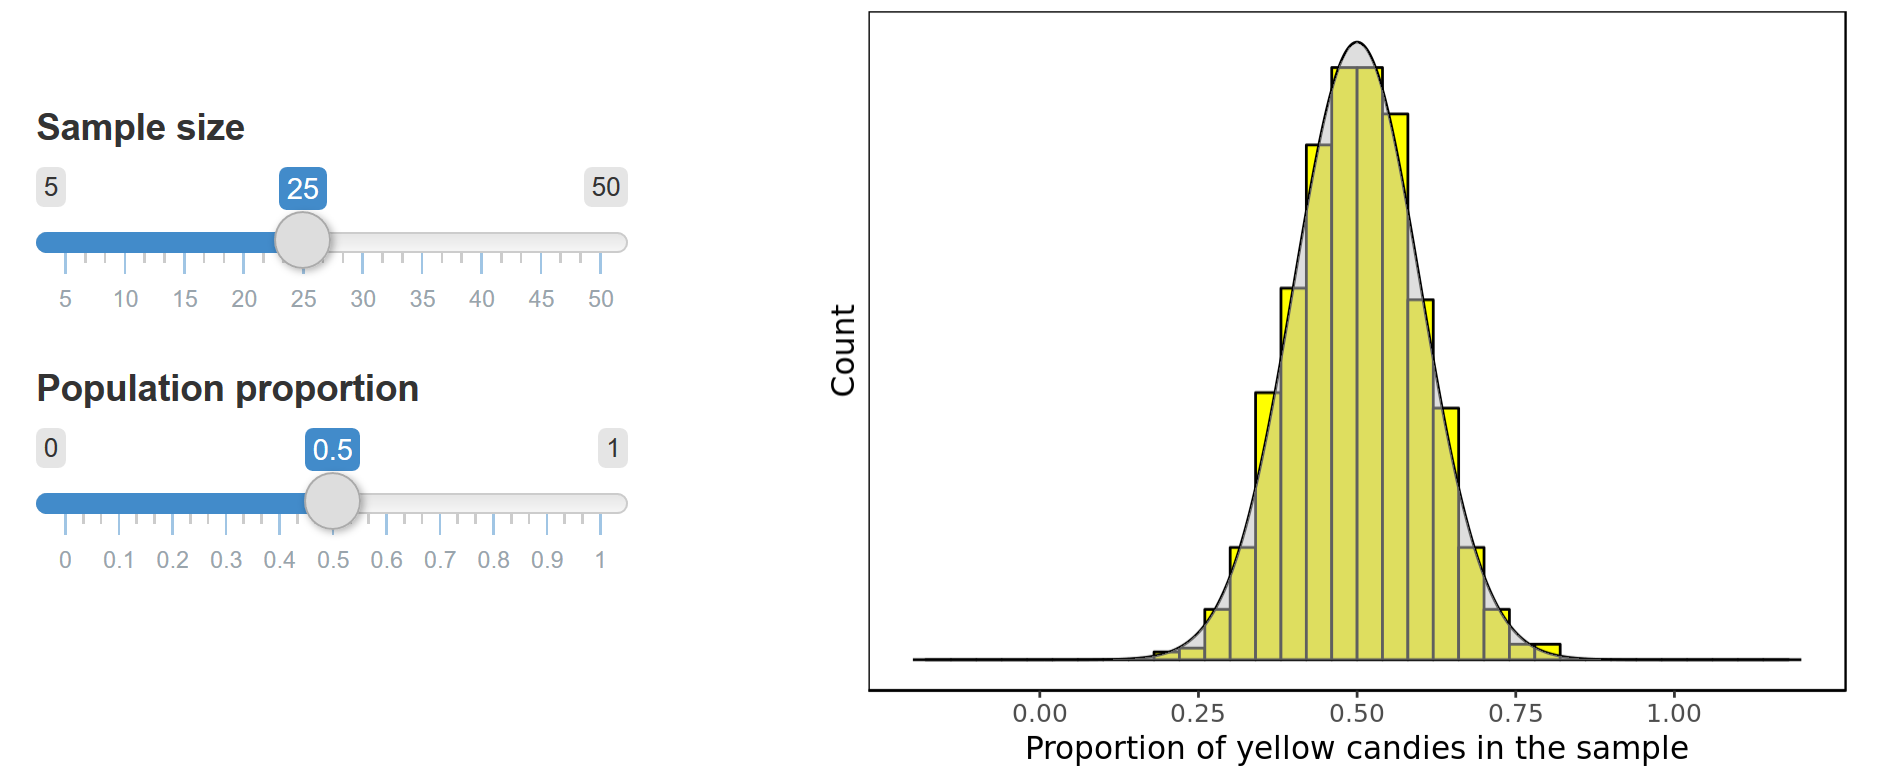
\includegraphics[width=320px]{GentleIntro_files/figure-latex/normal-approx-proportion-1} }\caption{How does the shape of the distribution of sample proportions change with sample size and proportion value?}\label{fig:normal-approx-proportion}
\end{figure}

\begin{enumerate}
\def\labelenumi{\arabic{enumi}.}
\tightlist
\item
  How do you expect that sample size affects the shape of the sampling
  distribution? State your expectation and then check it in the
  interactive content by changing sample size.
\end{enumerate}

\begin{Shaded}
\begin{Highlighting}[]
\OperatorTok{*}\StringTok{ }\NormalTok{The larger the sample, the more information each sample contains, the more}
\NormalTok{samples resemble the population, the closer is the sample statistic to the}
\NormalTok{population value. As a consequence, a larger sample produces a sampling}
\NormalTok{distribution with a lower }\KeywordTok{spread}\NormalTok{ (standard deviation, variance), so the}
\NormalTok{sampling distribution is more peaked.}
\end{Highlighting}
\end{Shaded}

\begin{enumerate}
\def\labelenumi{\arabic{enumi}.}
\setcounter{enumi}{1}
\tightlist
\item
  How do you expect that the value of the proportion in the population
  affects the shape of the sampling distribution? State your expectation
  and then check it in the interactive content by changing the
  population proportion.
\end{enumerate}

\begin{Shaded}
\begin{Highlighting}[]
\OperatorTok{*}\StringTok{ }\NormalTok{The population }\KeywordTok{proportion}\NormalTok{ (parameter value) is equal to the average of the}
\NormalTok{sampling distribution because the sample proportion is an unbiased estimator}
\NormalTok{of the population proportion. So }\ControlFlowTok{if}\NormalTok{ we change the population proportion, the}
\NormalTok{center of the sampling distribution changes accordingly.}
\OperatorTok{*}\StringTok{ }\NormalTok{In addition, the sampling distribution becomes less symmetrical}\OperatorTok{/}\NormalTok{more skewed}
\ControlFlowTok{if}\NormalTok{ the population proportion approaches zero or one. Because proportions}
\NormalTok{cannot be less than zero or more than one, the sampling distribution cannot}
\NormalTok{remain symmetrical }\ControlFlowTok{if}\NormalTok{ the population proportion is near zero or one.}
\end{Highlighting}
\end{Shaded}

Do theoretical probability distributions fit the true sampling
distribution? As you may have noticed while playing with Figure
\ref{fig:normal-approx-proportion}, this is not always the case. In
general, theoretical probability distributions fit sampling
distributions better if the sample is larger. In addition, the value of
the parameter may be relevant to the fit of the theoretical probability
distribution. The sampling distribution of a sample proportion is more
symmetrical, like the normal distribution, if the proportion in the
population is nearer .5.

This illustrates that we often have several conditions for a theoretical
probability distribution to fit the sampling distribution. We should
evaluate all of them at the same time. In the example of proportions, a
large sample is less important if the true proportion is closer to .5
but it is more important for true proportions that are more distant from
.5.

The rule of thumb for using the normal distribution as the sampling
distribution of a sample proportion combines the two aspects by
multiplying them and requiring the resulting product to be larger than
five. If the probability of drawing a yellow candy is .2 and our sample
size is 30, the product is .2 * 30 = 6, which is larger than five. So we
may use the normal distribution as approximation of the sampling
distribution.

Note that this rule of thumb uses one minus the probability, if the
probability is larger than .5. In other words, it uses the smaller of
two probabilities: the probability that an observation has the
characteristic and the probability that it has not. For example, if we
want to test the probability of drawing a candy that is not yellow, the
probability is .8 and we use 1 - 0.8 = 0.2, which is then multiplied by
the sample size.

Apart from the normal distribution, there are several other theoretical
probability distributions. We have the \emph{binomial distribution} for
a proportion, the \emph{t distribution} for one or two sample means,
regression coefficients, and correlation coefficients, the \emph{F
distribution} for comparison of variances and comparing means for three
or more groups (analysis of variance, ANOVA), and the \emph{chi-squared
distribution} for frequency tables and contingency tables.

For most of these theoretical probability distributions, sample size is
important. The larger the sample, the better. There are additional
conditions that must be satisfied such as the distribution of the
variable in the population. The rules of thumb are summarized in Table
\ref{tab:thumb}. Bootstrapping and exact tests can be used if conditions
for theoretical probability distributions have not been met. Special
conditions apply to regression analysis (see Chapter \ref{moderation},
Section \ref{regr-inference}).

\begin{table}

\caption{\label{tab:thumb}Rules of thumb for using theoretical probability distributions.}
\centering
\fontsize{8}{8}\selectfont
\begin{tabular}[t]{p{2.5cm}p{2.5cm}p{3.5cm}p{3.5cm}}
\hline
Distribution & Sample statistic & Minimum sample size & Other requirements\\
\hline
Binomial distribution & proportion & - & -\\
(Standard) normal distribution & proportion & >= 5 divided by test proportion (<= .5) & -\\
(Standard) normal distribution & one or two means & > 100 & OR variable is normally distributed in the population and population standard deviation is known (for each group)\\
t distribution & one or two means & each group > 30 & OR variable is normally distributed in each group's population\\
t distribution & (Pearson) correlation coefficient & - & variables are normally distributed in the population\\
t distribution & (Spearman) rank correlation coefficient & > 30 & -\\
t distribution & regression coefficient & 20+ per independent variable & See Chapter 8.\\
F distribution & 3+ means & all groups are more or less of equal size & OR all groups have the same population variance\\
F distribution & two variances & - & no conditions for Levene's F test\\
chi-squared distribution & row or cell frequencies & expected frequency >= 1 and 80\% >= 5 & contingency table: 3+ rows or 3+ columns\\
\hline
\end{tabular}
\end{table}

\subsection{Checking conditions}\label{checking-conditions}

Rules of thumb about sample size are easy to check once we have
collected our sample. By contrast, rules of thumb that concern the
scores in the population cannot be easily checked, because we do not
have information on the population. If we already know what we want to
know about the population, why would we draw a sample and do the
research in the first place?

We can only use the data in our sample to make an educated guess about
the distribution of a variable in the population. For example, if the
scores in our sample are clearly normally distributed, it is plausible
that the scores in the population are normally distributed.

In this situation, we do not \emph{know} that the population
distribution is normal but we \emph{assume} it is. If the sample
distribution is clearly not normally distributed, we had better not
assume that the population is normally distributed. In short, we
sometimes have to make assumptions when we decide on using a theoretical
probability distribution.

We could use a histogram of the scores in our sample with a normal
distribution curve added to evaluate whether a normal distribution
applies. Sometimes, we have statistical tests to draw inferences about
the population from a sample that we can use to check the conditions. We
discuss these tests in a later chapter.

\subsection{More complicated sample statistics:
differences}\label{complicatedsampling}

Up to this point, we have focused on rather simple sample statistics
such as the proportion of yellow candies or the average weight of
candies in a sample. Table \ref{tab:thumb}, however, contains more
complicated sample statistics.

If we compare two groups, for instance, the average weight of yellow and
red candies, the sample statistic for which we want to have a sampling
distribution must take into account both the average weight of yellow
candies and the average weight of red candies. The sample statistic that
we are interested in is the difference between the averages of the two
samples.

\begin{figure}[H]
\href{http://82.196.4.233:3838/apps/mean-independent/}{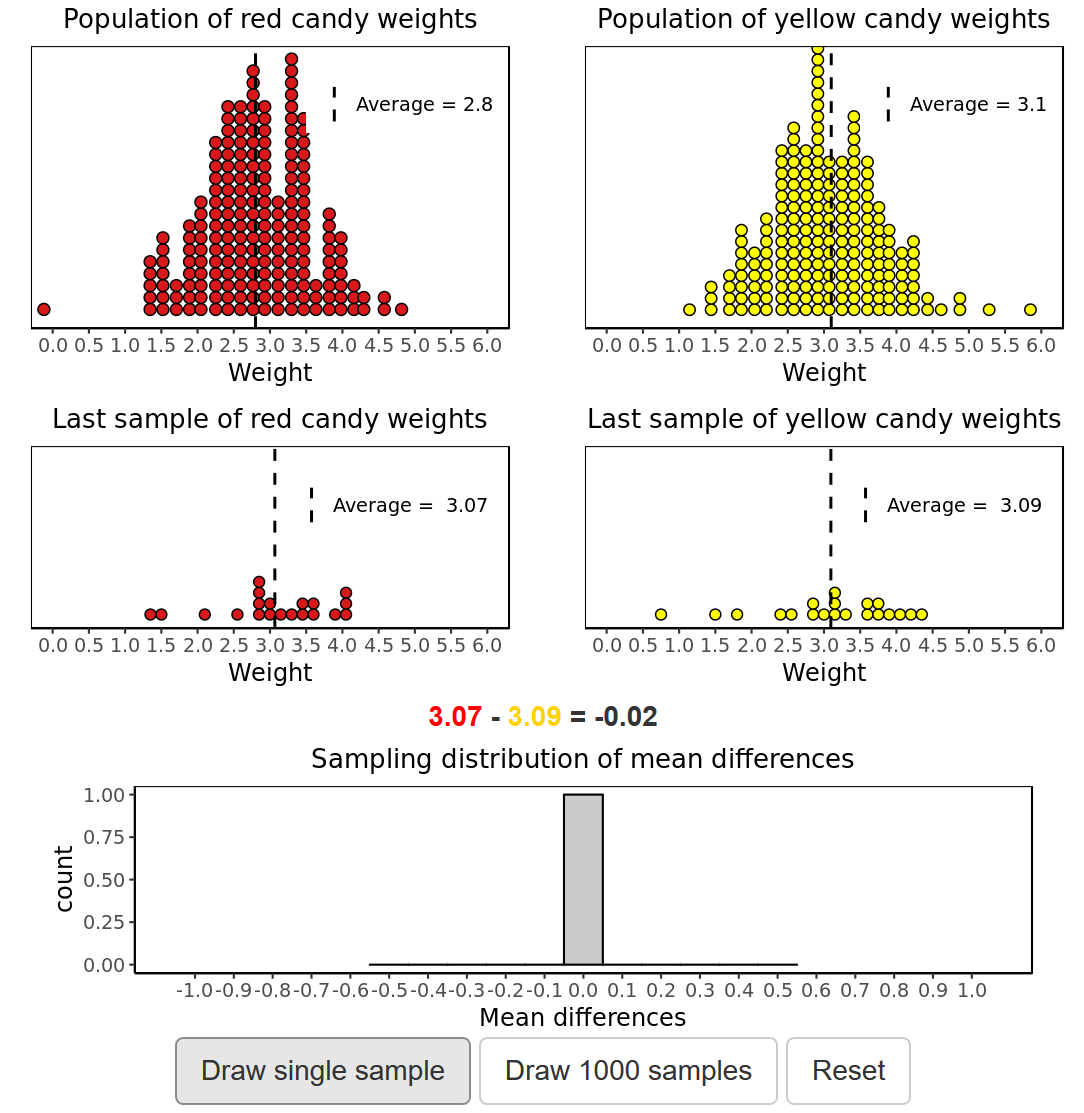
\includegraphics[width=550px]{GentleIntro_files/figure-latex/mean-independent-1} }\caption{How do we obtain a sampling distribution for the mean difference of two independent samples?}\label{fig:mean-independent}
\end{figure}

\begin{enumerate}
\def\labelenumi{\arabic{enumi}.}
\tightlist
\item
  Click on the button once. Why are these samples called independent?
\end{enumerate}

\begin{Shaded}
\begin{Highlighting}[]
\OperatorTok{*}\StringTok{ }\NormalTok{It is }\ControlFlowTok{in}\NormalTok{ principle possible to draw a random sample of red candies}
\NormalTok{separately from a random sample of yellow candies.}
\end{Highlighting}
\end{Shaded}

\begin{enumerate}
\def\labelenumi{\arabic{enumi}.}
\setcounter{enumi}{1}
\tightlist
\item
  Click on the button several times. What exactly is the sample
  statistic in the histogram at the bottom of the app?
\end{enumerate}

\begin{Shaded}
\begin{Highlighting}[]
\OperatorTok{*}\StringTok{ }\NormalTok{It is the difference between average weight of red candies and average}
\NormalTok{weight of yellow candies }\ControlFlowTok{in}\NormalTok{ a sample.}
\OperatorTok{*}\StringTok{ }\NormalTok{This is illustrated by the equation directly above the graph of the sampling}
\NormalTok{distribution, which subtracts the average weight of yellow }\KeywordTok{candies}\NormalTok{ (}\ControlFlowTok{in}\NormalTok{ yellow}
\NormalTok{typeface) from the average weight of red }\KeywordTok{candies}\NormalTok{ (}\ControlFlowTok{in}\NormalTok{ red typeface). The result}
\NormalTok{is added to the sampling distribution.}
\end{Highlighting}
\end{Shaded}

\begin{enumerate}
\def\labelenumi{\arabic{enumi}.}
\setcounter{enumi}{2}
\tightlist
\item
  Click on the button to draw one thousand samples once or more often.
  Does the sampling distribution look familiar to you?
\end{enumerate}

\begin{Shaded}
\begin{Highlighting}[]
\OperatorTok{*}\StringTok{ }\NormalTok{The sampling distribution has a bell shape like the normal }\KeywordTok{or}\NormalTok{ (Student) t}
\NormalTok{distribution.}
\end{Highlighting}
\end{Shaded}

\begin{enumerate}
\def\labelenumi{\arabic{enumi}.}
\setcounter{enumi}{3}
\tightlist
\item
  What, do you expect, is the mean of the sampling distribution?
\end{enumerate}

\begin{Shaded}
\begin{Highlighting}[]
\OperatorTok{*}\StringTok{ }\NormalTok{The true difference }\ControlFlowTok{in}\NormalTok{ averages }\ControlFlowTok{in}\NormalTok{ the population is what we expect as the}
\NormalTok{average difference }\ControlFlowTok{in}\NormalTok{ the sampling distribution.}
\OperatorTok{*}\StringTok{ }\NormalTok{Average weight of red candies }\ControlFlowTok{in}\NormalTok{ the population is }\FloatTok{2.8}\NormalTok{ grams and the average}
\NormalTok{weight }\ControlFlowTok{in}\NormalTok{ the population of yellow candies is }\FloatTok{3.1}\NormalTok{ gram. The average weight}
\NormalTok{difference }\ControlFlowTok{in}\NormalTok{ the population is }\FloatTok{2.8} \OperatorTok{-}\StringTok{ }\FloatTok{3.1}\NormalTok{ =}\StringTok{ }\OperatorTok{-}\FloatTok{0.3}\NormalTok{ gram. This is our}
\NormalTok{expectation.}
\OperatorTok{*}\StringTok{ }\NormalTok{The centre of the sampling distribution is indeed at }\OperatorTok{-}\FloatTok{0.3} \ControlFlowTok{if}\NormalTok{ we draw}
\NormalTok{thousands of samples.}
\end{Highlighting}
\end{Shaded}

If we draw a sample from both the red and yellow red candies in the
population, we may calculate the means for both samples and the
difference between the two means. For example, the average weight of red
candies in the sample bag is 2.76 gram and the average for yellow
candies is 2.82 gram. For this pair of samples, the statistic of
interest is 2.76 - 2.82 = -0.06, that is, the difference in average
weight. If we repeat this many, many times and collect all differences
between means in a distribution, we obtain the sampling distribution
that we need.

The sampling distribution of the difference between two means is similar
to a \emph{t}-distribution, so we may use the latter to approximate the
former. Of course, the conditions for using the \emph{t} distribution
must be met.

It is important to note that we do not create separate sampling
distributions for the average weight of yellow candies and for the
average weight of red candies and then look at the difference between
the two sampling distributions. Instead, we create \emph{one sampling
distribution for the statistic of interest}, namely the difference
between means. We cannot combine different sampling distributions into a
new sampling distribution. We will see the importance of this when we
discuss mediation (Chapter \ref{mediation}).

\subsection{Independent samples}\label{independent-samples}

If we compare two means, there are two fundamentally different
situations that are sometimes difficult to distinguish. When comparing
the average weight of yellow candies to the average weight of red
candies, we are comparing two samples that are \emph{statistically
independent} (see Figure \ref{fig:mean-independent}), which means that
we could have drawn the samples separately.

In principle, we could distinguish between a population of yellow
candies and a population of red candies, and sample yellow candies from
the first population and separately sample red candies from the other
population. Whether we sampled the colours separately or not does not
matter. The fact that we could have done so implies that the sample of
red candies is not affected by the sample of yellow candies or the other
way around. The samples are statistically independent.

This is important for the way in which probabilities are calculated.
Just think of the simple example of flipping two coins. The probability
of having heads twice in a row is .5 times .5, that is .25, if the coins
are unbiased and the result of the second coin does not depend on the
result of the first coin. The second flip is not affected by the first
flip.

Imagine that a magnetic field is activated if the first coin lands with
heads up and that this magnetic field increases the odds that the second
coin will also be heads. Now, the second toss is not independent of the
first toss and the probability of getting heads twice is larger than
.25.

\subsection{Dependent samples}\label{dependentsamples}

The example of a manipulated second toss is applicable to repeated
measurements. If we want to know how quickly the yellow colour fades
when yellow candies are exposed to sun light, we may draw a sample of
yellow candies once and measure the colourfulness of each candy at least
twice: at the start and end of some time interval. Subsequently, we
compare the average colourfulness of the second set of measurements to
the average in the first set of measurements.

\begin{figure}[H]
\href{http://82.196.4.233:3838/apps/mean-dependent/}{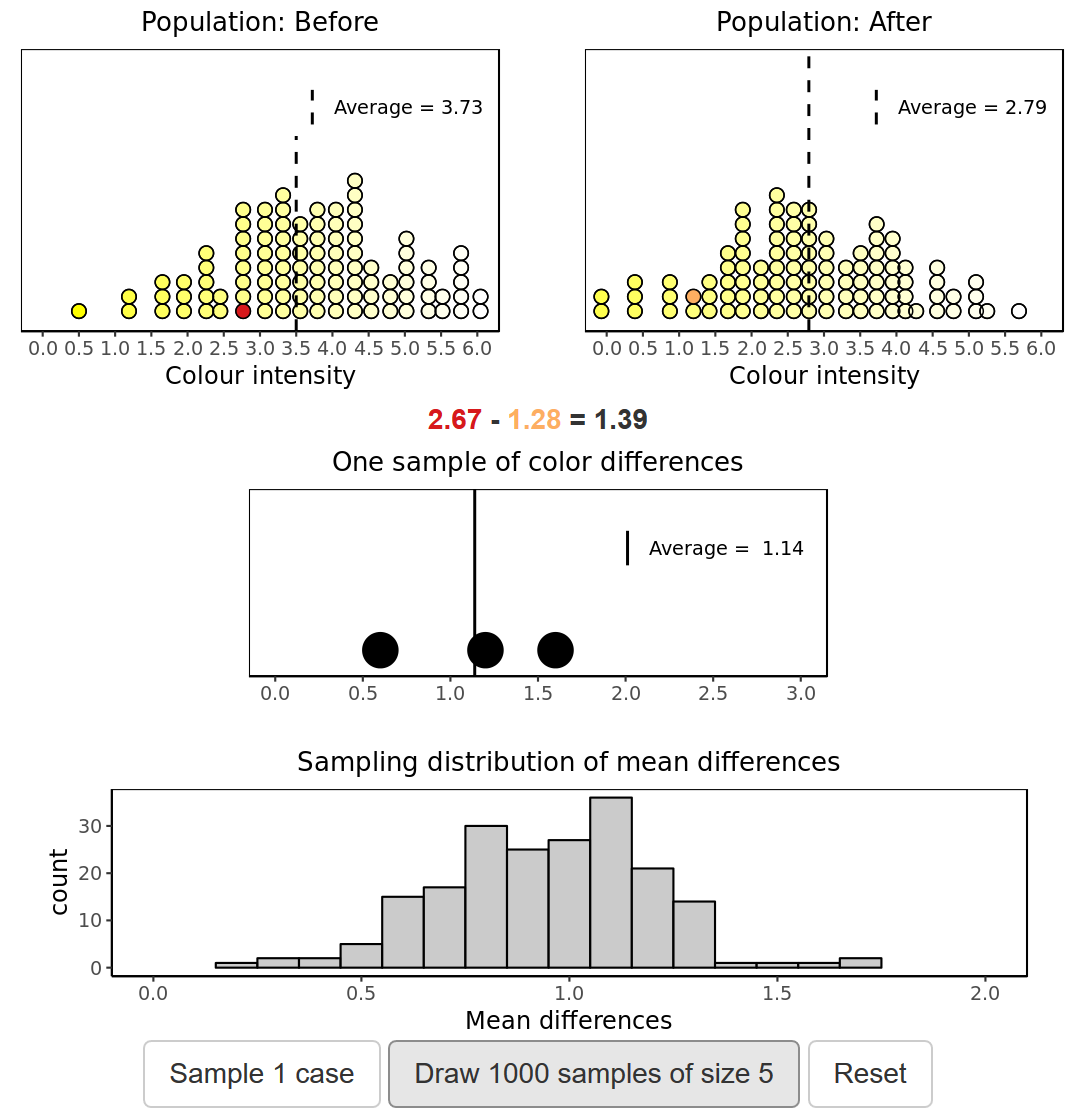
\includegraphics[width=560px]{GentleIntro_files/figure-latex/mean-dependent-1} }\caption{Dependent samples.}\label{fig:mean-dependent}
\end{figure}

\begin{enumerate}
\def\labelenumi{\arabic{enumi}.}
\tightlist
\item
  In Figure \ref{fig:mean-dependent}, use the \textbf{Sample 1 case}
  button repeatedly to draw a sample of five observations. What is the
  precise meaning of the numbers on the horizontal axis in the dot plot
  representing the sample (in the middle of Figure
  \ref{fig:mean-dependent})?
\end{enumerate}

\begin{Shaded}
\begin{Highlighting}[]
\OperatorTok{*}\StringTok{ }\NormalTok{The numbers on the horizontal axis }\ControlFlowTok{in}\NormalTok{ the sample histogram represent the}
\NormalTok{difference }\ControlFlowTok{in}\NormalTok{ colour intensity }\ControlFlowTok{for}\NormalTok{ each pair of cases that is drawn.}
\OperatorTok{*}\StringTok{ }\NormalTok{In each draw, one case }\ControlFlowTok{in}\NormalTok{ the before }\KeywordTok{population}\NormalTok{ (red) and the same case }\ControlFlowTok{in}
\NormalTok{the after }\KeywordTok{population}\NormalTok{ (orange) is selected. The difference }\ControlFlowTok{in}\NormalTok{ colour intensity}
\NormalTok{between the before and after measurement is calculated }\ControlFlowTok{in}\NormalTok{ the equation below}
\NormalTok{the population dot plots. The calculated difference }\ControlFlowTok{for}\NormalTok{ this pair is}
\NormalTok{represented by a dot }\ControlFlowTok{in}\NormalTok{ the figure }\ControlFlowTok{in}\NormalTok{ the middle.}
\end{Highlighting}
\end{Shaded}

\begin{enumerate}
\def\labelenumi{\arabic{enumi}.}
\setcounter{enumi}{1}
\tightlist
\item
  Why is the sample called dependent or paired?
\end{enumerate}

\begin{Shaded}
\begin{Highlighting}[]
\OperatorTok{*}\StringTok{ }\NormalTok{A case appears both }\ControlFlowTok{in}\NormalTok{ the before and after population}\OperatorTok{:}\StringTok{ }\NormalTok{We have a before and}
\NormalTok{after measurement of colour intensity }\ControlFlowTok{for}\NormalTok{ each }\KeywordTok{case}\NormalTok{ (candy). These two}
\NormalTok{measurements are related or paired because they refer to the same candy.}
\OperatorTok{*}\StringTok{ }\NormalTok{As a consequence, }\ControlFlowTok{if}\NormalTok{ we draw candies }\ControlFlowTok{for}\NormalTok{ our before measurement, we also draw}
\NormalTok{the candies }\ControlFlowTok{for}\NormalTok{ our after measurement. The after sample depends on the before}
\NormalTok{sample.}
\end{Highlighting}
\end{Shaded}

\begin{enumerate}
\def\labelenumi{\arabic{enumi}.}
\setcounter{enumi}{2}
\tightlist
\item
  Draw 1,000 samples to obtain a sampling distribution. What is the
  precise meaning of the numbers on the horizontal axis in the histogram
  of the sampling distribution?
\end{enumerate}

\begin{Shaded}
\begin{Highlighting}[]
\OperatorTok{*}\StringTok{ }\NormalTok{The numbers on the horizontal axis }\ControlFlowTok{in}\NormalTok{ the histogram of the sampling}
\NormalTok{distribution signify the average difference }\ControlFlowTok{in}\NormalTok{ colour intensity of the candies}
\ControlFlowTok{in}\NormalTok{ a }\KeywordTok{sample}\NormalTok{ (of five candies).}
\end{Highlighting}
\end{Shaded}

In this example, we are comparing two means, just like the yellow versus
red candy weight example, but now the samples for both measurements are
the same. It is impossible to draw the sample for the second measurement
independently from the sample for the first measurement if we want to
compare repeated measurements. Here, the second sample is fixed once we
have drawn the first sample. The samples are \emph{statistically
dependent}; they create \emph{paired samples}. Even if the second sample
depends only partly upon the first sample, the samples are statistically
dependent.

With dependent samples, probabilities have to be calculated in a
different way, so we need a special sampling distribution. In the
interactive content above, you may have noticed a relatively simple
solution for two repeated measurements. We just calculate the difference
between the two measurements for each candy in the sample and use the
mean of this new difference variable as the sample statistic that we are
interested in. The \emph{t}-distribution, again, offers a good
approximation of the sampling distribution of dependent samples if the
samples are not too small.

For other applications, the actual sampling distributions can become
quite complicated but we need not worry about that. If we choose the
right technique, our statistical software will take care of this.

\section{SPSS and Theoretical Approximation of the Sampling
Distribution}\label{spss-and-theoretical-approximation-of-the-sampling-distribution}

By default, SPSS uses a theoretical probability distribution to
approximate the sampling distribution. It chooses the correct
theoretical distribution but you yourself should check if the conditions
for using this distribution are met. For example, is the sample large
enough or is it plausible that the variable is normally distributed in
the population?

In one case, SPSS automatically selects an exact approach if the
conditions for a theoretical approximation are not met. If you do a
chi-squared test to a contingency table in SPSS, SPSS will automatically
apply Fisher's exact test if the table has two rows and two columns. In
all other cases, you have to select a bootstrapping or exact approach
yourself if the conditions for a theoretical approximation are not met.

We are not going to practice with theoretical approximations in SPSS,
now. Because theoretical approximation is the default approach in SPSS,
we will encounter it in the exercises in later chapters.

\section{When Do We Use Which Approach to the Sampling
Distribution?}\label{when-do-we-use-which-approach-to-the-sampling-distribution}

By default, SPSS uses a theoretical approximation of the sampling
distribution. Select the right test in SPSS and SPSS ensures that an
appropriate theoretical probability distribution is used. You, however,
must check whether the sample meets the conditions for using this
theoretical probability distribution, see Table \ref{tab:thumb}.

If the conditions for using a theoretical probability distribution are
not met, we use bootstrapping or an exact approach. An exact approach is
available only if the variables are categorical. Sometimes, for example
in a two by two cross tabulation, SPSS automatically uses an exact
approach. Otherwise, you have to request an exact test or bootstrapping
yourself.

Finally, we also use bootstrapping if SPSS does not have a test for the
statistic in which we are interested. For example, if we want to
estimate or test the median value or the standard deviation of a
variable.

\section{Test Your Understanding}\label{test-your-understanding-1}

\begin{figure}[H]
\href{http://82.196.4.233:3838/apps/bootstrapping/}{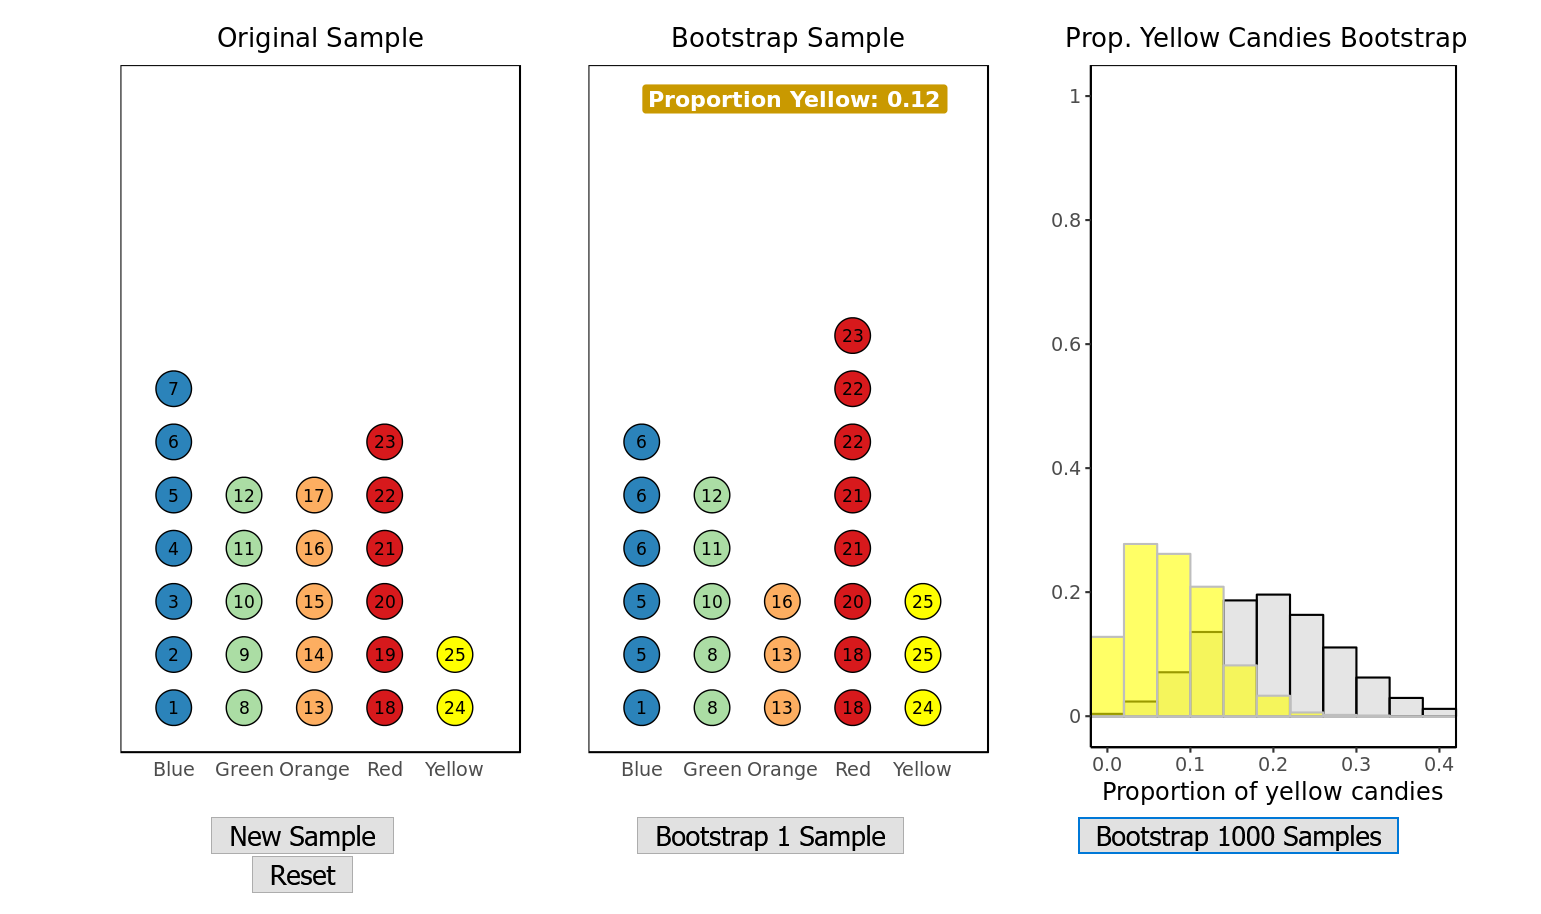
\includegraphics[width=420px]{GentleIntro_files/figure-latex/models-summary1-1} }\caption{How do we bootstrap a sampling distribution?}\label{fig:models-summary1}
\end{figure}

\begin{enumerate}
\def\labelenumi{\arabic{enumi}.}
\tightlist
\item
  Why does Figure \ref{fig:models-summary1} not show a population?
\end{enumerate}

\begin{Shaded}
\begin{Highlighting}[]
\OperatorTok{*}\StringTok{ }\NormalTok{With bootstrapping, we create a sampling distribution by sampling}
\NormalTok{(}\StringTok{"bootstrapping"}\NormalTok{) from our initial sample. Therefore, we do not need the}
\NormalTok{original population }\ControlFlowTok{for}\NormalTok{ bootstrapping.}
\end{Highlighting}
\end{Shaded}

\begin{enumerate}
\def\labelenumi{\arabic{enumi}.}
\setcounter{enumi}{1}
\tightlist
\item
  Which type of sampling is better here: with or without replacement?
  Justify your answer.
\end{enumerate}

\begin{Shaded}
\begin{Highlighting}[]
\OperatorTok{*}\StringTok{ }\NormalTok{The bootstrap sample must contain the same number of observations as the}
\NormalTok{original sample because the sampling distribution depends on sample size. }
\OperatorTok{*}\StringTok{ }\NormalTok{If we draw bootstrap samples without replacement from the original sample,}
\NormalTok{every observation }\ControlFlowTok{in}\NormalTok{ the original sample can be sampled only once. To obtain a}
\NormalTok{bootstrap sample that is just as large as the original sample, then, we must}
\NormalTok{use all observations from the original sample. As a result, the bootstrap}
\NormalTok{sample is identical to the original sample. All bootstrap samples are identical}
\NormalTok{to the original sample, so we do not have variation }\ControlFlowTok{in}\NormalTok{ the sampling}
\NormalTok{distribution.}
\OperatorTok{*}\StringTok{ }\NormalTok{Only }\ControlFlowTok{if}\NormalTok{ we sample with replacement, bootstrap samples can be different from}
\NormalTok{the initial sample, so we obtain a sampling distribution with variation, that}
\NormalTok{is, allowing }\ControlFlowTok{for}\NormalTok{ different sample outcomes. And this is what we need a}
\NormalTok{sampling distribution for.}
\end{Highlighting}
\end{Shaded}

\begin{enumerate}
\def\labelenumi{\arabic{enumi}.}
\setcounter{enumi}{2}
\tightlist
\item
  Draw a new initial sample in Figure \ref{fig:models-summary1}. Is the
  bootstrapped sampling distribution going to resemble the true sampling
  distribution? Note that twenty per cent of the candies in the
  population are yellow. Motivate your answer. Draw 1,000 bootstrap
  samples to check your answer.
\end{enumerate}

\begin{Shaded}
\begin{Highlighting}[]
\OperatorTok{*}\StringTok{ }\NormalTok{A bootstrapped sampling distribution only resembles the true sampling}
\NormalTok{distribution }\ControlFlowTok{if}\NormalTok{ the initial sample is more or less representative of the}
\NormalTok{population. The sample statistic that we are interested }\ControlFlowTok{in}\NormalTok{, }\ControlFlowTok{in}\NormalTok{ the current}
\NormalTok{example, the proportion of yellow candies, must be quite near the population}
\NormalTok{statistic.}
\OperatorTok{*}\StringTok{ }\NormalTok{If the proportion of yellow samples }\ControlFlowTok{in}\NormalTok{ the original sample is .}\DecValTok{2}\NormalTok{, as it is}
\ControlFlowTok{in}\NormalTok{ the population, the bootstrapped sampling }\KeywordTok{distribution}\NormalTok{ (yellow) is very}
\NormalTok{similar to the true sampling }\KeywordTok{distribution}\NormalTok{ (black curve). Another proportion of}
\NormalTok{yellow candies }\ControlFlowTok{in}\NormalTok{ the original sample, however, produces a sampling}
\NormalTok{distribution that does not resemble the true sampling distribution.}
\end{Highlighting}
\end{Shaded}

\begin{table}[H]

\caption{\label{tab:models-summary-3}Number of heads for a toss of three coins.}
\centering
\fontsize{8}{8}\selectfont
\begin{tabular}[t]{cl}
\hline
Number of heads & Combination\\
\hline
0 & tail-tail-tail\\
1 & tail-tail-head\\
1 & tail-head-tail\\
1 & head-tail-tail\\
2 & head-head-tail\\
2 & head-tail-head\\
2 & tail-head-head\\
3 & head-head-head\\
\hline
Total & 8\\
\hline
\end{tabular}
\end{table}

\begin{enumerate}
\def\labelenumi{\arabic{enumi}.}
\setcounter{enumi}{3}
\tightlist
\item
  Calculate the exact probability distribution of the number of heads in
  a toss of three fair coins (Table \ref{tab:models-summary-3}).
\end{enumerate}

\begin{Shaded}
\begin{Highlighting}[]
\OperatorTok{*}\StringTok{ }\NormalTok{For the answer, see Section Exact Approaches to the Sampling Distribution.}
\end{Highlighting}
\end{Shaded}

\begin{enumerate}
\def\labelenumi{\arabic{enumi}.}
\setcounter{enumi}{4}
\tightlist
\item
  In which situations can we use exact probabilities as a sampling
  distribution?
\end{enumerate}

\begin{Shaded}
\begin{Highlighting}[]
\OperatorTok{*}\StringTok{ }\NormalTok{We must be able to list and count all combinations. This can only be done }\ControlFlowTok{if}
\NormalTok{the number of combinations is limited. So we need discrete or categorical}
\NormalTok{variables. Exact approaches to the sampling distribution are only available}
\ControlFlowTok{for}\NormalTok{ inference on categorical variables, such as proportions and associations.}
\end{Highlighting}
\end{Shaded}

\begin{figure}[H]
\href{http://82.196.4.233:3838/apps/normal-approximation/}{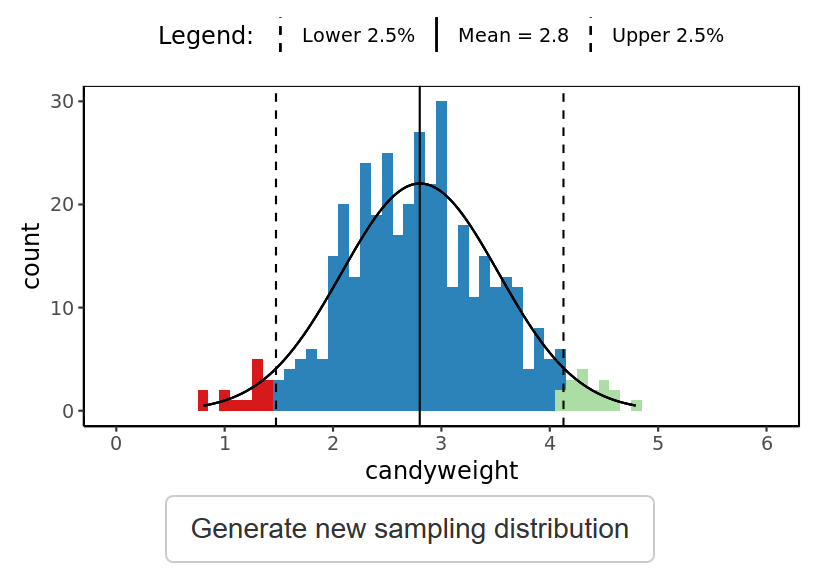
\includegraphics[width=420px]{GentleIntro_files/figure-latex/models-summary2-1} }\caption{How do we approximate a sampling distribution with a theoretical probability distribution?}\label{fig:models-summary2}
\end{figure}

\begin{enumerate}
\def\labelenumi{\arabic{enumi}.}
\setcounter{enumi}{5}
\tightlist
\item
  Generate a sampling distribution of average sample candy weight in
  Figure \ref{fig:models-summary2}. Try to explain in your own words why
  the sampling distribution of a sample mean has a bell shape.
\end{enumerate}

\begin{Shaded}
\begin{Highlighting}[]
\OperatorTok{*}\StringTok{ }\NormalTok{Samples with means close to the true population mean are more likely than}
\NormalTok{samples with means far away from the true population mean because observations}
\NormalTok{(candy weights) above average tend to be balanced by observations below}
\NormalTok{average. This explains the top at the true population mean.}
\OperatorTok{*}\StringTok{ }\NormalTok{It is equally likely to draw a sample with above average mean score as a}
\NormalTok{sample with below average mean score, so the sampling distribution is}
\NormalTok{symmetric around the true population value.}
\end{Highlighting}
\end{Shaded}

\begin{enumerate}
\def\labelenumi{\arabic{enumi}.}
\setcounter{enumi}{6}
\tightlist
\item
  Which part of the graph in Figure \ref{fig:models-summary2} represents
  the theoretical probability distribution and what is the name of this
  distribution?
\end{enumerate}

\begin{Shaded}
\begin{Highlighting}[]
\OperatorTok{*}\StringTok{ }\NormalTok{The black }\KeywordTok{curve}\NormalTok{ (or the surface below the black curve) represents the}
\NormalTok{theoretical probability distribution. It is a normal }\KeywordTok{or}\NormalTok{ (Student) t}
\NormalTok{distribution.}
\end{Highlighting}
\end{Shaded}

\begin{enumerate}
\def\labelenumi{\arabic{enumi}.}
\setcounter{enumi}{7}
\tightlist
\item
  Does this theoretical probability distribution always fit the
  simulated sampling distribution in Figure \ref{fig:models-summary2}?
  Create several sampling distributions and explain why we pay special
  attention to the lowest (red) and highest (green) 2.5\% of the sample
  means.
\end{enumerate}

\begin{Shaded}
\begin{Highlighting}[]
\OperatorTok{*}\StringTok{ }\NormalTok{The curve fits the histogram of observed sample means quite well.}
\NormalTok{Discrepancies are mainly due to the jagged layout of the histogram, which}
\NormalTok{result from binning the }\KeywordTok{data}\NormalTok{ (to create bars) and from the fact that the}
\NormalTok{number of samples is large but not very large.}
\OperatorTok{*}\StringTok{ }\NormalTok{The borders demarcating the lowest and highest }\FloatTok{2.5}\NormalTok{% of sample means }\ControlFlowTok{in}\NormalTok{ the}
\NormalTok{theoretical probability }\KeywordTok{distribution}\NormalTok{ (the dotted lines) nicely coincide with}
\NormalTok{the border between red or green and blue bars }\ControlFlowTok{in}\NormalTok{ the histogram }\ControlFlowTok{in}\NormalTok{ most of the}
\NormalTok{sampling distributions that we generate with this app.}
\OperatorTok{*}\StringTok{ }\NormalTok{These borders are important because we use them }\ControlFlowTok{for}\NormalTok{ confidence intervals and}
\ControlFlowTok{for}\NormalTok{ statistical tests.}
\end{Highlighting}
\end{Shaded}

\section{Take-Home Points}\label{take-home-points-1}

\begin{itemize}
\item
  We may create an exact sampling distribution or simulate a bootstrap
  sampling distribution in simple situations or if we have a lot of
  computing power.
\item
  For a bootstrap sampling distribution, we need about 5,000 bootstrap
  samples from our original sample.
\item
  We can often approximate the sampling distribution of a sample
  statistic with a known theoretical probability distribution.
\item
  Approximations only work well under conditions, which we have to
  check.
\item
  Conditions usually involve the size of the sample, sample type
  (independent vs.~dependent/paired), and the shape or variance of the
  population distribution.
\item
  If these conditions are not met or we do not have a theoretical
  approximation to the sampling distribution, we use bootstrapping or
  exact tests.
\item
  Samples are independent if, in principle, we can draw a sample for one
  group without taking into account the sample for another group of
  cases. Otherwise, the samples are dependent or paired.
\end{itemize}

\chapter{Estimating a Parameter: Which Population Values Are
Plausible?}\label{param-estim}

\begin{quote}
Key concepts: point estimate, interval estimate, confidence (level),
precision, standard error, critical value, confidence interval.
\end{quote}

\subsection*{Summary}\label{summary-2}
\addcontentsline{toc}{subsection}{Summary}

\begin{quote}
Given our sample, what are plausible population values?
\end{quote}

In this chapter, we set out to make educated guesses of a population
value (parameter, often called ``the true value'') based on our sample.
This type of guessing is called \emph{estimation}. Our first guess will
be a single value for the population value. We merely guess that the
population value is equal to the value of the sample statistic. This
guess is the most precise guess that we can make, but it is most likely
to be wrong.

Our second guess uses the sampling distribution to make a statement
about the approximate population value. More precisely, we calculate an
interval for which we are confident that it includes the population
value. We can increase our confidence by widening the interval, but this
decreases the precision of our guess.

\section{Point Estimate}\label{point-estimate}

If we have to name one value for the population value, our best guess is
the value of the sample statistic. For example, if 18\% of the candies
in our sample bag are yellow, our best guess of the proportion of yellow
candies in the population of all candies from which this bag was filled,
is .18. What other number can we give if we only have our sample? This
type of guess is called a \emph{point estimate} and we use it a lot.

The sample statistic is the best estimate of the population value only
if the sample statistic is an unbiased estimator of the population
value. As we have learned in Section \ref{unbiased-est}, the true
population value is equal to the mean of the sampling distribution for
an unbiased estimator. The mean of the sampling distribution is the
expected value for the sample.

In other words, an unbiased estimator neither systematically
overestimates the population value, nor does it systematically
underestimate the population value. With an unbiased estimator, then,
there is no reason to prefer a value higher or lower than the sample
value as our estimate of the population value.

Even though the value of the statistic in the sample is our best guess,
it is very unlikely that our sample statistic is exactly equal to the
population value (parameter). The recurrent theme in our discussion of
random samples is that a random sample differs from the population
because of chance during the sampling process. The precise population
value is highly unlikely to actually appear in our sample.

The sample statistic value is our best point estimate but it is nearly
certain to be wrong. It may be slightly or strongly off the mark but it
will hardly ever be spot on. For this reason, it is better to estimate a
range within which the population value falls. Let us turn to this in
the next section.

\section{Interval Estimate for the Sample
Statistic}\label{interval-estimate-for-the-sample-statistic}

The sampling distribution of a continuous sample statistic tells us the
probability of finding a range of scores for the sample statistic in a
random sample. For example, the average weight of candies in a sample
bag is a continuous random variable. The sampling distribution tells us
the probability of drawing a sample with average candy weight between
2.0 and 3.6 gram. We can use this range as our \emph{interval estimate}.

Note that we are reasoning from sampling distribution to sample now.
This is not what we want to do in actual research, where we want to
reason from sample to sampling distribution to population. We get to
that in Section \ref{ci-parameter}. For now, assume that we know the
true sampling distribution.

Remember that the average or expected value of a sampling distribution
is equal to the population value if the estimator is unbiased. For
example, the mean weight of yellow candies averaged over a very large
number of samples is equal to the mean weight of yellow candies in the
population. For an interval estimate, we now select the sample statistic
values that are closest to the average of the sampling distribution.

Between which boundaries do we find the sample statistic values that are
closest to the population value? Of course, we have to specify what we
mean by ``closest''. Which part of all samples do we want to include? A
popular proportion is 95\%, so we want to know the boundary values that
include 95\% of all samples that are closest to the population value.
For example, between which boundaries is average candy weight situated
for 95\% of all samples that are closest to the average candy weight in
the population?

\begin{figure}[H]
\href{http://82.196.4.233:3838/apps/ci-borders/}{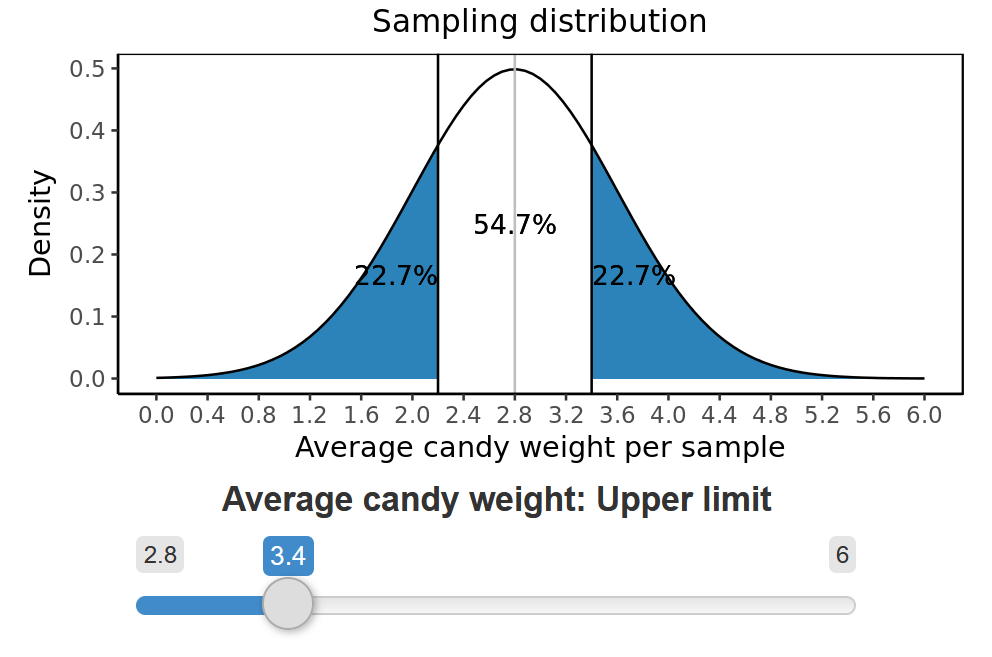
\includegraphics[width=420px]{GentleIntro_files/figure-latex/ci-borders-1} }\caption{Within which interval do we find the sample results that are closest to the population value?}\label{fig:ci-borders}
\end{figure}

Figure \ref{fig:ci-borders} shows the sampling distribution of average
sample candy weight.

\begin{enumerate}
\def\labelenumi{\arabic{enumi}.}
\tightlist
\item
  What is the average candy weight in the population of candies?
\end{enumerate}

\begin{Shaded}
\begin{Highlighting}[]
\OperatorTok{*}\StringTok{ }\NormalTok{A sample mean is an unbiased estimator of the population mean. As a}
\NormalTok{consequence, the mean of the sampling distribution is equal to the population }
\NormalTok{value, }\ControlFlowTok{in}\NormalTok{ this case the population mean.}
\OperatorTok{*}\StringTok{ }\KeywordTok{The}\NormalTok{ (normal) sampling distribution is symmetrical, so the mean of the}
\NormalTok{sampling distribution is }\ControlFlowTok{in}\NormalTok{ the middle, exactly under the top of the sampling}
\NormalTok{distribution. Here, the value is }\FloatTok{2.8}\NormalTok{ (gram). This is average candy weight }\ControlFlowTok{in}
\NormalTok{the population.}
\end{Highlighting}
\end{Shaded}

\begin{enumerate}
\def\labelenumi{\arabic{enumi}.}
\setcounter{enumi}{1}
\tightlist
\item
  Move the slider until you have found the interval containing 95\% of
  all samples that are closest to the (true) population value. What are
  the upper and lower limits of the interval that contains these
  samples?
\end{enumerate}

\begin{Shaded}
\begin{Highlighting}[]
\OperatorTok{*}\StringTok{ }\NormalTok{The exact value of the }\KeywordTok{upper}\NormalTok{ (right) limit changes from application to}
\NormalTok{application. It usually is somewehere between }\DecValTok{3}\NormalTok{ and }\DecValTok{5}\NormalTok{. }
\OperatorTok{*}\StringTok{ }\NormalTok{To obtain the exact }\KeywordTok{lower}\NormalTok{ (left) limit, calculate the difference between the}
\NormalTok{upper limit and the mean of the }\KeywordTok{distribution}\NormalTok{ (}\FloatTok{2.8}\NormalTok{). Then subtract this}
\NormalTok{difference from the distribution }\KeywordTok{mean}\NormalTok{ (}\FloatTok{2.8}\NormalTok{) to get the }\KeywordTok{lower}\NormalTok{ (sleft) limit of}
\NormalTok{the interval.}
\OperatorTok{*}\StringTok{ }\NormalTok{Tip}\OperatorTok{:}\StringTok{ }\NormalTok{If the cursor is on the slider handle, you can change the slider value}
\ControlFlowTok{in}\NormalTok{ minimal steps with the left and right arrow keys on your keyboard.}
\end{Highlighting}
\end{Shaded}

Say, for instance, that 95\% of all possible samples in the middle of
the sampling distribution have an average candy weight ranging from 1.6
to 4.0 gram. The proportion .95 can be interpreted as a probability. Our
sampling distribution tells us that we have 95\% probability that the
average weight of yellow candies lies between 1.6 and 4.0 gram in a
random sample that we draw from this population.

We now have boundary values, that is, a range of sample statistic
values, and a probability of drawing a sample with a statistic falling
within this range. The probability shows our \emph{confidence} in the
estimate. It is called the \emph{confidence level} of an interval
estimate.

\section{Precision, Standard Error, and Sample
Size}\label{precisionsesamplesize}

The width of the estimated interval represents the \emph{precision} of
our estimate. The wider the interval, the less precise our estimate.
With a less precise interval estimate, we will have to reckon with a
wider variety of outcomes in our sample.

\begin{figure}[H]
\href{http://82.196.4.233:3838/apps/interval-level/}{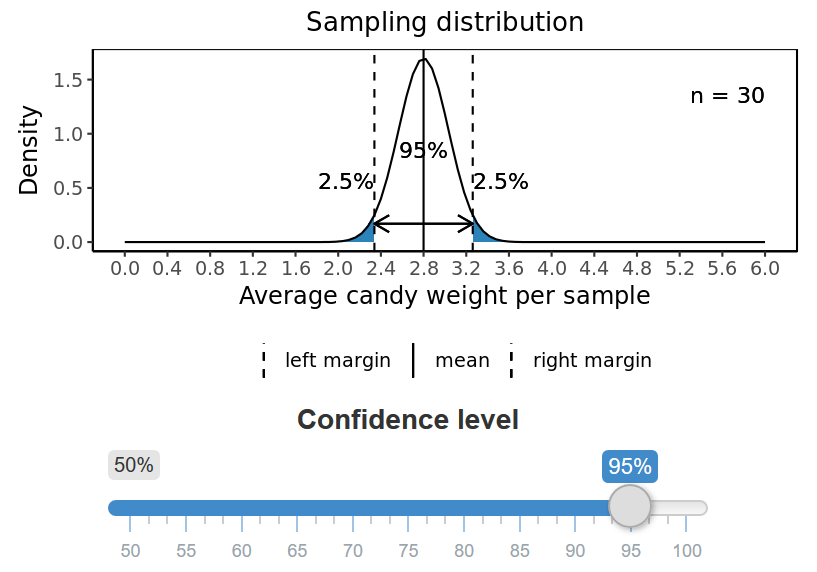
\includegraphics[width=420px]{GentleIntro_files/figure-latex/interval-level-1} }\caption{How does the confidence level affect the precision of an interval estimate?}\label{fig:interval-level}
\end{figure}

\begin{enumerate}
\def\labelenumi{\arabic{enumi}.}
\tightlist
\item
  How, do you think, does the precision (width) of the interval estimate
  (represented by the double-sided arrow) change if you change the
  confidence level? First write down what you expect, and why you expect
  that. Then check what happens if you change the confidence level
  slider in Figure \ref{fig:interval-level}.
\end{enumerate}

\begin{Shaded}
\begin{Highlighting}[]
\OperatorTok{*}\StringTok{ }\NormalTok{The lower our confidence level, the more population values we exclude, the}
\NormalTok{narrower the interval estimate}\OperatorTok{:}\StringTok{ }\NormalTok{precision is higher. }
\OperatorTok{*}\StringTok{ }\NormalTok{The higher our confidence level, the more population values we include, the}
\NormalTok{broader the interval estimate}\OperatorTok{:}\StringTok{ }\NormalTok{precision is smaller.}
\end{Highlighting}
\end{Shaded}

\begin{enumerate}
\def\labelenumi{\arabic{enumi}.}
\setcounter{enumi}{1}
\tightlist
\item
  What happens if we want to be 100\% certain that our interval contains
  the true population value?
\end{enumerate}

\begin{Shaded}
\begin{Highlighting}[]
\OperatorTok{*}\StringTok{ }\NormalTok{If we want to be }\DecValTok{100}\NormalTok{% sure, we cannot rule out any possible average weight}
\NormalTok{as the true population value. As a consequence, the interval becomes}
\NormalTok{infinitely wide. Of course, such an interval is completely useless because it}
\NormalTok{tells us that any value is possible.}
\end{Highlighting}
\end{Shaded}

If we want to predict something, we value precision. We rather conclude
that the average weight of candies in the next sample we draw lies
between 2.0 and 3.6 gram than between 1.6 and 4.0 gram. If we would be
satisfied with a very imprecise estimate, we need not do any research at
all. With relatively little knowledge about the candies that we are
investigating, we could straightaway predict that the average candy
weight is between zero and ten gram. The goal of our research is to find
a more precise estimate.

There are several ways to increase the precision of our interval
estimate, that is, to obtain a narrower interval for our estimate. The
easiest and least useful way is to decrease our confidence that our
estimate is correct. If we lower the confidence that we are right, we
can discard a large number of other possible sample statistic outcomes
and focus on a narrower range of sample outcomes around the true
population value.

This method is not useful because we sacrifice our confidence that the
range includes the outcome in the sample that we are going to draw. What
is the use of a more precise estimate if we are less certain that it
predicts correctly? Therefore, we usually do not change the confidence
level and leave it at 95\% or thereabouts (90\%, 99\%). It is important
to be quite sure that our prediction will be right.

\subsection{Sample size}\label{sample-size}

A less practical but very useful method of narrowing the interval
estimate is increasing sample size. If we buy a larger bag containing
more candies, we get a better idea of average candy weight in the
population.

\begin{figure}[H]
\href{http://82.196.4.233:3838/apps/interval-size/}{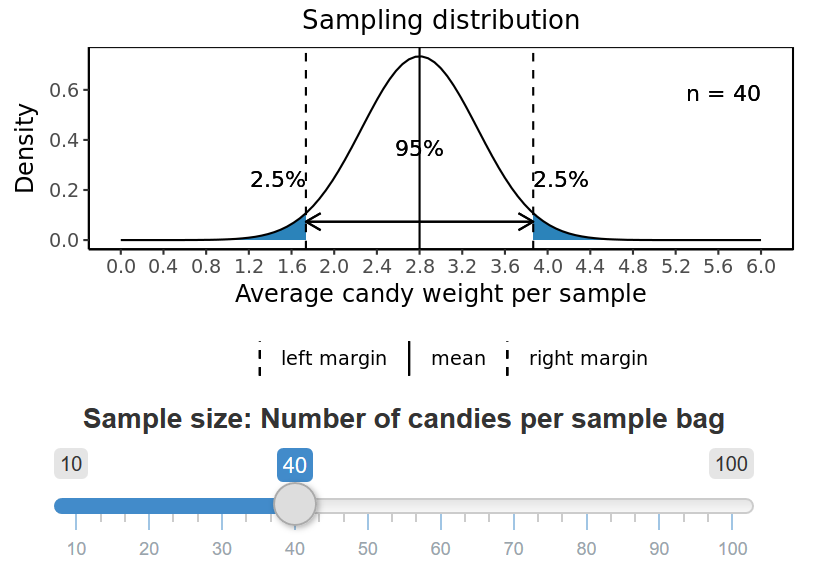
\includegraphics[width=420px]{GentleIntro_files/figure-latex/interval-size-1} }\caption{How does sample size affect the precision of an interval estimate?}\label{fig:interval-size}
\end{figure}

Figure \ref{fig:interval-size} shows a sampling distribution of average
candy weight in candy sample bags. The horizontal arrow indicates the
precision of the interval estimate.

\begin{enumerate}
\def\labelenumi{\arabic{enumi}.}
\tightlist
\item
  How does the precision of the interval estimate change if you change
  the size of the sample? First write down what you expect, and why you
  expect that. Then, check what happens if you change the sample size
  slider.
\end{enumerate}

\begin{Shaded}
\begin{Highlighting}[]
\OperatorTok{*}\StringTok{ }\NormalTok{Larger samples offer more information, so they allow a more precise estimate}
\NormalTok{of a population value, such as average candy weight. The precision of the}
\NormalTok{interval will increase, so the interval will become narrower, the arrow will}
\NormalTok{become shorter.}
\OperatorTok{*}\StringTok{ }\NormalTok{The computational reason}\OperatorTok{:}\StringTok{ }\NormalTok{A larger sample yields a smaller standard error}
\NormalTok{(se). See the }\ControlFlowTok{next}\NormalTok{ section.}
\end{Highlighting}
\end{Shaded}

\begin{enumerate}
\def\labelenumi{\arabic{enumi}.}
\setcounter{enumi}{1}
\tightlist
\item
  How does the shape of the sampling distribution change if you change
  sample size? Explain what this means for the values of the sample
  statistic.
\end{enumerate}

\begin{Shaded}
\begin{Highlighting}[]
\OperatorTok{*}\StringTok{ }\NormalTok{Remember that the sampling distribution represents the sample statistic}
\NormalTok{scores of all possible samples. The percentages, therefore, express the share}
\NormalTok{of samples with particular scores.}
\OperatorTok{*}\StringTok{ }\NormalTok{If a larger part of all sample means are found near }\KeywordTok{the}\NormalTok{ (true) population}
\NormalTok{mean, which happens }\ControlFlowTok{for}\NormalTok{ larger samples, the sampling distribution becomes more}
\NormalTok{peaked}\OperatorTok{/}\NormalTok{less flat.}
\end{Highlighting}
\end{Shaded}

As you may have noticed while playing with Figure
\ref{fig:interval-size}, a larger sample yields a narrower, that is,
more precise interval. You may have expected intuitively that larger
samples give more precise estimates because they offer more information.
This intuition is correct.

In a larger sample, an observation above the mean is more likely to be
compensated by an observation below the mean. Just because there are
more observations, it is less likely that we sample relatively high
scores but no or considerably fewer scores that are relatively low.

The larger the sample, the more the distribution of scores for a
variable in the sample will resemble the distribution of scores for this
variable in the population. As a consequence, a sample statistic value
will be closer to the population value for this statistic.

Larger samples resemble the population more closely, and therefore large
samples drawn from the same population are also closer to one another.
The result is that the sample statistic values in the sampling
distribution are less varied and more similar. They are more
concentrated around the true population value, which is the average of
the sampling distribution. The middle 95\% of all sample statistic
values are closer to the centre, so the sampling distribution is more
peaked.

\subsection{Standard error}\label{standard-error}

The concentration of sample statistic values, such as average candy
weight in a sample bag, around the centre (mean) of the sampling
distribution is expressed by the standard deviation of the sampling
distribution. Hitherto, we have only paid attention to the centre of the
sampling distribution, its mean, because it is the expected value in a
sample and it is equal to the population value if the estimator is
unbiased.

Now, we start looking at the standard deviation of the sampling
distribution as well, because it tells us how precise our interval
estimate is going to be. The sampling distribution's standard deviation
is so important that it has received a special name: the \emph{standard
error}.

\begin{figure}[H]
\href{http://82.196.4.233:3838/apps/se-point-est/}{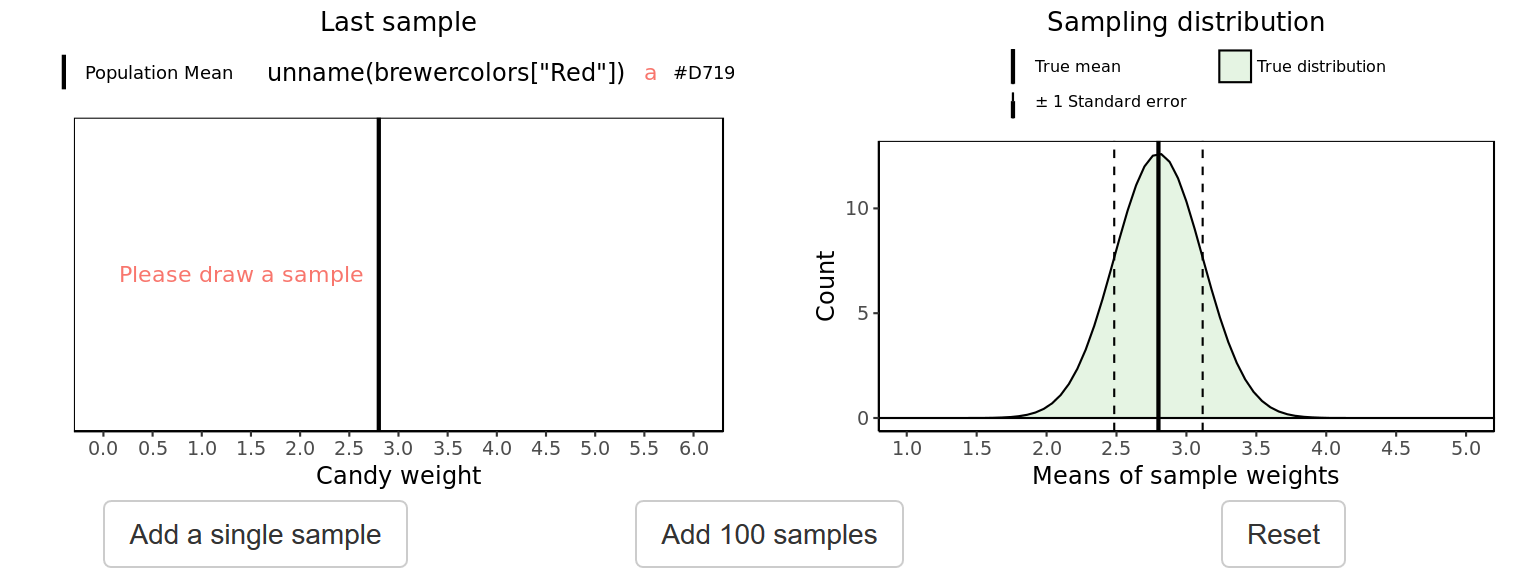
\includegraphics[width=320px]{GentleIntro_files/figure-latex/se-point-est-1} }\caption{The standard error: How wrong are point estimates?}\label{fig:se-point-est}
\end{figure}

\begin{enumerate}
\def\labelenumi{\arabic{enumi}.}
\tightlist
\item
  Draw a single sample by pressing the button \emph{Take single sample}
  in Figure \ref{fig:se-point-est}. Explain why we can interpret the red
  arrow in the sample plot (top graph) as estimation error.
\end{enumerate}

\begin{Shaded}
\begin{Highlighting}[]
\OperatorTok{*}\StringTok{ }\NormalTok{We use the sample }\KeywordTok{mean}\NormalTok{ (represented by the dotted line }\ControlFlowTok{in}\NormalTok{ the top graph) as}
\NormalTok{point estimate }\ControlFlowTok{for}\NormalTok{ the population }\KeywordTok{mean}\NormalTok{ (represented by the solid line). The}
\NormalTok{distance between the two shows how wrong our point estimate is. For this}
\NormalTok{reason, the red arrow }\ControlFlowTok{in}\NormalTok{ the top chart can be regarded as the size of the}
\NormalTok{estimation error.}
\end{Highlighting}
\end{Shaded}

\begin{enumerate}
\def\labelenumi{\arabic{enumi}.}
\setcounter{enumi}{1}
\tightlist
\item
  Use the button \textbf{Take single sample} several times. What is the
  meaning of the double-sided red arrow that appears in the sampling
  distribution?
\end{enumerate}

\begin{Shaded}
\begin{Highlighting}[]
\OperatorTok{*}\StringTok{ }\NormalTok{The double}\OperatorTok{-}\NormalTok{sided red arrow expresses the standard deviation of the sample}
\NormalTok{means that we have added to the sampling }\KeywordTok{distribution}\NormalTok{ (according to the}
\NormalTok{legend). So it is the standard deviation }\ControlFlowTok{in}\NormalTok{ the empirical sampling}
\NormalTok{distribution that we create by repeated sampling.}
\OperatorTok{*}\StringTok{ }\NormalTok{It gives an impression of how different the means of different random}
\NormalTok{samples can be. Because those sample means are used as point estimates, the}
\NormalTok{red arrow expresses }\KeywordTok{the}\NormalTok{ (average) size of the errors that we make }\ControlFlowTok{if}\NormalTok{ we}
\NormalTok{generalize the sample mean to the population mean.}
\end{Highlighting}
\end{Shaded}

\begin{enumerate}
\def\labelenumi{\arabic{enumi}.}
\setcounter{enumi}{2}
\tightlist
\item
  Use the button \textbf{Take 100 samples} once or repeatedly. What
  happens to the length of the double-sided red arrow in the sampling
  distribution?
\end{enumerate}

\begin{Shaded}
\begin{Highlighting}[]
\OperatorTok{*}\StringTok{ }\NormalTok{The red arrow fits the distance between the dotted lines }\ControlFlowTok{in}\NormalTok{ the bottom plot.}
\NormalTok{The dotted lines mark one standard error above or below the mean of the true}
\NormalTok{sampling }\KeywordTok{distribution}\NormalTok{ (light green). The arrowheads of the red arrows mark one}
\NormalTok{standard deviation above and below the average of the sample means that we}
\NormalTok{have drawn.}
\OperatorTok{*}\StringTok{ }\NormalTok{The standard error of a sampling distribution, then, is equal to the}
\NormalTok{standard deviation of the sampling distribution.}
\end{Highlighting}
\end{Shaded}

The word \emph{error} reminds us that the standard error tells us the
size of the error that we are likely to make (on average under many
repetitions) if we use the value of the sample statistic as a point
estimate for the population value.

Let us assume, for instance, that the standard error of the average
weight of candies in a sample bag is 0.6. Loosely stated, this means
that the average difference between true average candy weight and
average candy weight in a sample is 0.6 if we draw a very large number
of samples from the same population.

The smaller the standard error, the more the sample statistic values
resemble the true population value, and the more precise our interval
estimate is with a given confidence level, for instance, 95\%. Because
we like more precise interval estimates, we prefer small standard errors
over high standard errors.

It is easy to obtain smaller standard errors: just increase sample size.
See Figure \ref{fig:interval-size}, where larger samples yield more
peaked sampling distributions. In a peaked distribution, values are
closer to the mean and the standard error is smaller. In our example,
average candy weights in larger sample bags are closer to the average
candy weight in the population.

In practice, however, it is both time-consuming and expensive to draw a
very large sample. Usually, we want to settle on the optimal size of the
sample, namely a sample that is large enough to have interval estimates
at the confidence level and precision that we need but as small as
possible to save on time and expenses. We return to this matter in
Chapter \ref{power}.

The standard error may also depend on other factors, such as the
variation in population scores. In our example, more variation in the
weight of candies in the population produces a larger standard error for
the average candy weight in a sample bag. If there are more very heavy
candies and very light candies, it is easier to draw a sample with
several heavy candies or with several very light candies. Average weight
in these sample bags will be too high or too low. We cannot influence
the variation in candy weights in the population, so let us ignore this
factor influencing the standard error.

\section{Critical Values}\label{crit-values}

In the preceding section, we learned that the standard error is related
to the precision of the interval estimate. A larger standard error
yields a less precise estimate, that is, with a wider confidence
interval.

We are interested in the interval that includes a particular percentage
of all samples that can be drawn, usually the 95 per cent of all samples
that are closest to the population value. In our current example, the 95
per cent of all samples with average candy weight that is closest to
average candy weight in the population (2.8 gram).

In theoretical probability distributions like the normal distribution,
the percentage of samples is related to the standard error. If we know
the standard error, we know the interval within which we find the 95 per
cent of samples that are closest to the population value.

\begin{figure}[H]
\href{http://82.196.4.233:3838/apps/crit-values/}{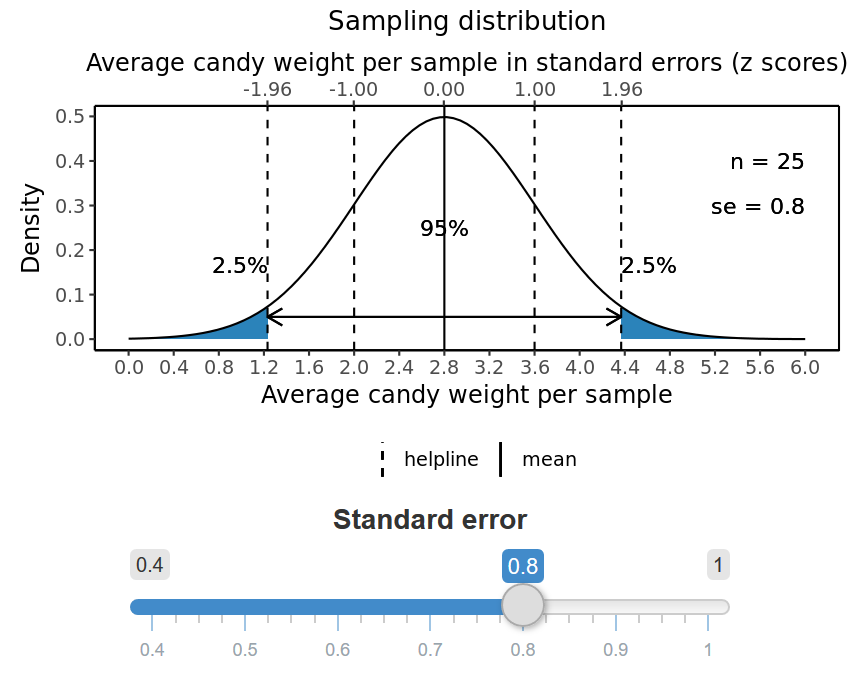
\includegraphics[width=440px]{GentleIntro_files/figure-latex/crit-values-1} }\caption{How do critical values relate to the standard error in a normal distribution?}\label{fig:crit-values}
\end{figure}

Figure \ref{fig:crit-values} shows the sampling distribution of average
candy weight per sample bag. It contains two horizontal axes, one with
average candy weight in grams (bottom) and one with average candy weight
in standard errors, also called \emph{z} scores (top).

\begin{enumerate}
\def\labelenumi{\arabic{enumi}.}
\tightlist
\item
  How do the two horizontal axes tell you the size of the standard error
  in grams?
\end{enumerate}

\begin{Shaded}
\begin{Highlighting}[]
\OperatorTok{*}\StringTok{ }\NormalTok{The axis at the bottom gives average candy weight }\ControlFlowTok{in}\NormalTok{ grams and the axis at}
\NormalTok{the top shows average candy weight }\ControlFlowTok{in}\NormalTok{ standard errors from the population}
\NormalTok{mean.}
\OperatorTok{*}\StringTok{ }\NormalTok{One standard error equals the distance or difference between z score zero}
\NormalTok{(}\DecValTok{0}\NormalTok{) and z score }\KeywordTok{one}\NormalTok{ (}\DecValTok{1}\NormalTok{). If we follow the lines down from these standard error}
\NormalTok{scores, we obtain the mean average candy }\KeywordTok{weight}\NormalTok{ (}\FloatTok{2.8}\NormalTok{ gram) and the average}
\NormalTok{weight one standard error above the }\KeywordTok{mean}\NormalTok{ (}\FloatTok{3.6}\NormalTok{ gram).}
\OperatorTok{*}\StringTok{ }\NormalTok{The difference is }\FloatTok{0.8}\NormalTok{ gram, so one standard error represents }\FloatTok{0.8} \KeywordTok{grams}\NormalTok{ (}\ControlFlowTok{in}
\NormalTok{average candy weight per sample bag). This is indeed the initial value on the}
\NormalTok{slider.}
\end{Highlighting}
\end{Shaded}

\begin{enumerate}
\def\labelenumi{\arabic{enumi}.}
\setcounter{enumi}{1}
\tightlist
\item
  How do you expect the location of the vertical lines to change if you
  change the size of the standard error? Check your expectation by using
  the slider.
\end{enumerate}

\begin{Shaded}
\begin{Highlighting}[]
\OperatorTok{*}\StringTok{ }\NormalTok{If we increase the standard error, one standard error coincides with more}
\NormalTok{grams, so the sampling distribution grows wider; it becomes less peaked. The}
\NormalTok{variation }\ControlFlowTok{in}\NormalTok{ sample }\KeywordTok{outcomes}\NormalTok{ (average candy weight) will increase.}
\OperatorTok{*}\StringTok{ }\NormalTok{The dotted lines representing plus or minus }\FloatTok{1.00}\NormalTok{ and }\FloatTok{1.96}\NormalTok{ will move away}
\NormalTok{from the centre but the centre will be fixed at the true average candy weight}
\ControlFlowTok{in}\NormalTok{ the population, }\ControlFlowTok{in}\NormalTok{ this example }\FloatTok{2.8}\NormalTok{ gram.}
\end{Highlighting}
\end{Shaded}

In Figure \ref{fig:crit-values}, we approximate the sampling
distribution with a theoretical probability distribution, namely the
normal distribution. The theoretical probability distribution links
probabilities (areas under the curve) to sample statistic outcome values
(scores on the horizontal axis). For example, we have 2.5\% probability
to draw a sample bag with average candy weight below 1.2 gram or 2.5\%
probability to draw a sample bag with average candy weight over 4.4
gram.

\subsection{\texorpdfstring{Standardization and \emph{z}
scores}{Standardization and z scores}}\label{standardization-and-z-scores}

The average candy weights that are associated with 2.5\% and 97.5\%
probabilities in Figure \ref{fig:crit-values} depend on the sample that
we have drawn. As you will have noticed while playing with Figure
\ref{fig:interval-size}, changing the size of the sample also changes
the average candy weights that mark the 2.5\% and 97.5\% probabilities.

We can simplify the situation if we \emph{standardize} the sampling
distribution: Subtract the average of the sampling distribution from
each sample mean in this distribution, and divide the result by the
standard error. Thus, we transform the sampling distribution into a
distribution of standardized scores. The mean of the new standardized
variable is always zero.

If we use the normal distribution for standardized scores, which is
called the \emph{standard-normal distribution} or \emph{z distribution},
there is a single \emph{z} value that marks the boundary between the top
2.5\% and the bottom 97.5\% of any sample. This \emph{z} value is 1.96.
If we combine this value with -1.96, separating the bottom 2.5\% of all
samples from the rest, we obtain an interval {[}-1.96, 1.96{]}
containing 95\% of all samples that are closest to the mean of the
sampling distribution. This is part of the \emph{empirical rule} for the
normal distribution.

In a standard-normal or \emph{z} distribution, 1.96 is called a
\emph{critical value}. Together with its negative (-1.96), it separates
the 95\% sample statistic outcomes that are closest to the parameter,
hence that are most likely to appear, from the 5\% that are furthest
away and least likely to appear. There are also critical \emph{z} values
for other probabilities, for instance, 1.64 for the middle 90\% of all
samples and 2.58 for the middle 99\% in a standard-normal distribution.

\subsection{Interval estimates from critical values and standard
errors}\label{int-est-sample-mean}

Critical values in a theoretical probability distribution tell us the
boundaries, or range, of the interval estimate expressed in standard
errors. In a normal distribution, 95\% of all sample means are situated
no more than 1.96 standard errors from the population mean.

If the standard error is 0.5 and the population mean is 2.8 gram, we
have 95\% probability that the mean candy weight in a sample that we
draw from this population lies between 1.82 gram (this is 1.96 times 0.5
subtracted from 2.8) and 3.78 gram.

Critical values make it easy to calculate an interval estimate if we
know the standard error. Just take the population value and add the
critical value times the standard error to obtain the upper limit of the
interval estimate. Subtract the critical value times the standard error
from the population value to obtain the lower limit.

Normal distributions make life easier for us, because there is a fixed
critical value for each probability, such as 1.96 for 95\% probability,
which is well-worth memorizing.

\section{Confidence Interval for a Parameter}\label{ci-parameter}

Working through the preceding sections, it may have occurred to you that
it is all very well to be able to estimate the value of a statistic in a
new sample with a particular precision and probability, but that this is
not what we are primarily interested in. Instead, we want to estimate
the value of the statistic in the population.

For example, we don't care much about the average weight of candies in
our sample bag or in the next sample bag that we may buy. We want to say
something about the average weight of candies in the population. How can
we do this?

In addition, you may have realized that, if we know the sampling
distribution, we also know the precise population value, for instance,
average candy weight. After all, the average of the sampling
distribution is equal to the population mean for an unbiased estimator.
In the preceding paragraphs, we acted as if we knew the sampling
distribution. If we know the sampling distribution, and it then follows
that we also know the population value, why would we even care about
estimating an interval?

Our problem is this: We want to estimate a population value using
probabilities. For probabilities we need the sampling distribution but
for the sampling distribution, we must know the population. A vicious
circle.

\begin{figure}
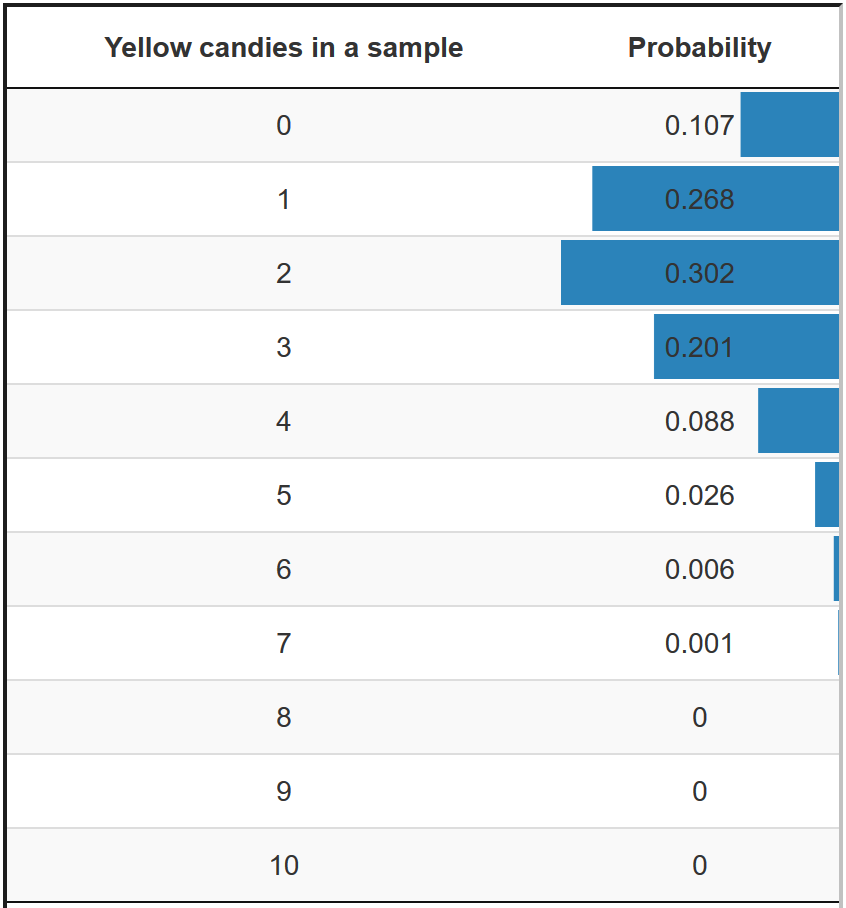
\includegraphics[width=200px]{figures/exactapproach} \caption{Probabilities of a sample with a particular number of yellow candies if 20 per cent of the candies are yellow in the population.}\label{fig:exactapproachfigure}
\end{figure}

In the exact approach to the sampling distribution of the proportion of
yellow candies in a sample bag (Figure \ref{fig:exactapproachfigure}),
for instance, we must know the proportion of yellow candies in the
population. If we know the population proportion, we can exactly
calculate the probability of getting a sample bag with a particular
proportion of yellow candies. But we don't know the population
proportion of yellow candies; we want to estimate it.

A theoretical probability distribution can only be used as an
approximation of a sampling distribution if we know some characteristics
of the population. We know that the sampling distribution of sample
means always has the bell shape of a normal (\emph{z}) distribution or
\emph{t} distribution. However, knowing the shape is not sufficient for
using the theoretical distribution as an approximation of the sampling
distribution.

We must also know the population mean because it specifies where the
centre of the sampling distribution is located. So, we must know the
population mean to use a theoretical probability distribution to
estimate the population mean. This sounds like a problem that only Baron
von Münchhausen can solve. How can we drag ourselves by the hair out of
this swamp?

By the way, we also need the standard error to know how peaked or flat
the bell shape is. The standard error can usually be estimated from the
data in our sample. But let us not worry about how the standard error is
being estimated and focus on estimating the population mean.

\subsection{Imaginary population values}\label{imag-pop-values}

How can we find plausible population means? Figure
\ref{fig:pop-means-ci} shows average candy weight in a random sample
(lower scale). Click somewhere under the top axis to select a possible
value for the population mean. The app will then display the interval of
most plausible sample means (green if it contains the actual sample
means, red otherwise) if this would be the true population value. In
addition, it calculates the \emph{z} value of the actual sample mean if
the selected value would be the true population value.

\begin{figure}[H]
\href{http://82.196.4.233:3838/apps/pop-means-ci/}{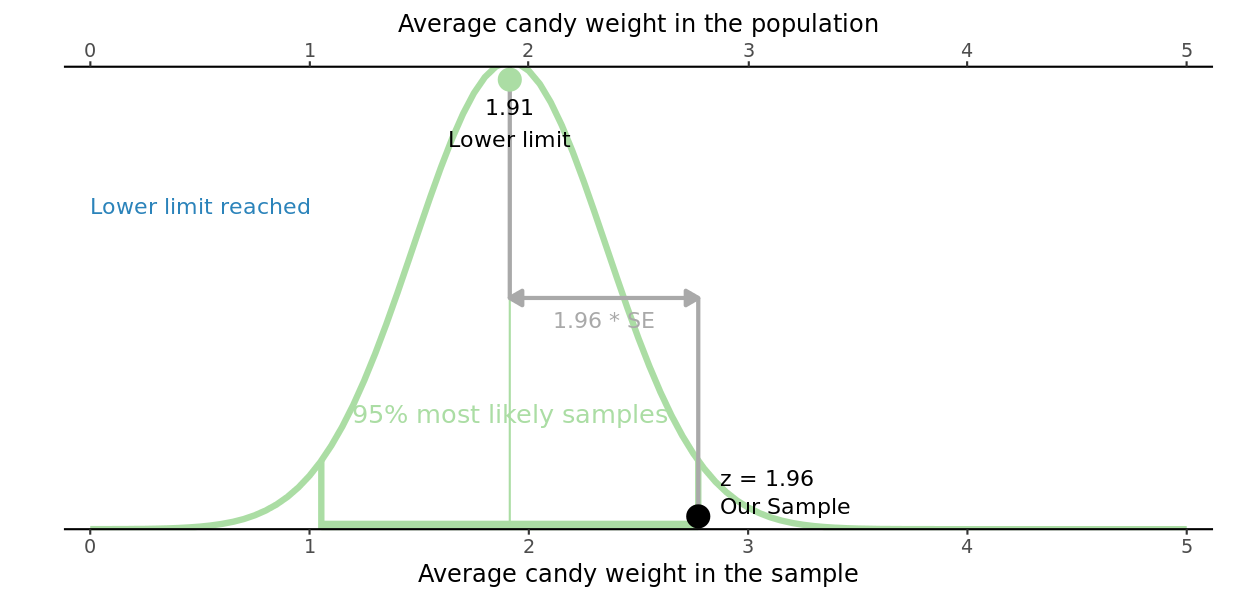
\includegraphics[width=630px]{GentleIntro_files/figure-latex/pop-means-ci-1} }\caption{For which population means is our sample mean plausible?}\label{fig:pop-means-ci}
\end{figure}

\begin{enumerate}
\def\labelenumi{\arabic{enumi}.}
\tightlist
\item
  Click repeatedly on Figure \ref{fig:pop-means-ci} to find the highest
  and lowest value of the population mean for which the sample mean is
  in the interval of sample means that have 95\% probability to occur.
\end{enumerate}

\begin{Shaded}
\begin{Highlighting}[]
\OperatorTok{*}\StringTok{ }\NormalTok{The closer the sample mean is to the population mean, the higher the}
\NormalTok{probability to draw a sample with more or less this mean. Population means}
\NormalTok{close to the sample mean will turn up as green dots and their intervals will}
\NormalTok{include the sample mean.}
\OperatorTok{*}\StringTok{ }\NormalTok{The more we move away from the sample mean, the less likely to draw a sample}
\NormalTok{with a mean that differs at least this much from the population mean. At some}
\NormalTok{point, the population mean is too far away from the sample mean, so the actual}
\NormalTok{sample mean is no longer within the range of the }\DecValTok{95}\NormalTok{% most likely sample means to}
\NormalTok{be drawn from a population with the selected population mean.}
\end{Highlighting}
\end{Shaded}

\begin{enumerate}
\def\labelenumi{\arabic{enumi}.}
\setcounter{enumi}{1}
\tightlist
\item
  How does the \emph{z} value of the sample mean help you to minimize
  the number of clicks you need?
\end{enumerate}

\begin{Shaded}
\begin{Highlighting}[]
\OperatorTok{*}\StringTok{ }\NormalTok{In a normal distribution, z standardizes scores and }\DecValTok{95}\NormalTok{% of all observations}
\NormalTok{differ no more than }\FloatTok{1.96}\NormalTok{ z scores from the mean. The lowest and highest}
\NormalTok{population means }\ControlFlowTok{for}\NormalTok{ which the current sample mean is among the }\DecValTok{95}\NormalTok{% most}
\NormalTok{plausible samples, then, are reached }\ControlFlowTok{if}\NormalTok{ the z value of the sample mean is}
\NormalTok{(almost) }\FloatTok{1.96}\NormalTok{ or }\OperatorTok{-}\FloatTok{1.96}\NormalTok{.}
\OperatorTok{*}\StringTok{ }\NormalTok{So the z value tells us how close we are to the limit.}
\end{Highlighting}
\end{Shaded}

\begin{enumerate}
\def\labelenumi{\arabic{enumi}.}
\setcounter{enumi}{2}
\tightlist
\item
  How does the depicted interval estimate help you to minimize the
  number of clicks you need?
\end{enumerate}

\begin{Shaded}
\begin{Highlighting}[]
\OperatorTok{*}\StringTok{ }\NormalTok{The interval estimate shows the width of the interval between the lowest and}
\NormalTok{highest population average }\ControlFlowTok{for}\NormalTok{ which the current sample mean is among the }\DecValTok{95}\NormalTok{%}
\NormalTok{most plausible samples.}
\OperatorTok{*}\StringTok{ }\NormalTok{If the current sample mean is at the left limit of the interval, we reach}
\NormalTok{the highest population mean }\ControlFlowTok{for}\NormalTok{ which the sample mean is within the interval.}
\NormalTok{Increase the population mean and the interval will no longer include the}
\NormalTok{current sample mean. In a similar way, the lowest population mean }\ControlFlowTok{for}\NormalTok{ which}
\NormalTok{the interval includes the sample mean is found }\ControlFlowTok{if}\NormalTok{ the sample mean is on the}
\NormalTok{right limit of the interval.}
\end{Highlighting}
\end{Shaded}

\begin{enumerate}
\def\labelenumi{\arabic{enumi}.}
\setcounter{enumi}{3}
\tightlist
\item
  What is the most efficient strategy (minimum number of clicks) to
  determine the lower and upper limits of the population means for which
  the sample mean is among the 95\% most likely samples? Explain why
  this is the most efficient strategy.
\end{enumerate}

\begin{Shaded}
\begin{Highlighting}[]
\OperatorTok{*}\StringTok{ }\NormalTok{Using the answer to Question }\DecValTok{3}\NormalTok{, we may use the following steps to find the}
\NormalTok{lower and upper limits.}
\NormalTok{a. Click }\ControlFlowTok{in}\NormalTok{ the middle of the sample mean. This selects the population mean}
\NormalTok{that is equal to the sample mean.}
\NormalTok{b. Click on the left edge of the interval. This should }\KeywordTok{be}\NormalTok{ (very near to) the}
\NormalTok{lowest population mean, the interval of which still includes the sample mean.}
\NormalTok{c. Repeat Step a to display again the interval }\ControlFlowTok{for}\NormalTok{ the population mean that is}
\NormalTok{equal to the sample mean.}
\NormalTok{d. Click the right end of this interval to find the highest population mean}
\NormalTok{such that the current sample mean is still among the }\DecValTok{95}\NormalTok{% most plausible}
\NormalTok{samples.}
\OperatorTok{*}\StringTok{ }\NormalTok{You may not hit the nail spot}\OperatorTok{-}\NormalTok{on with every click but the procedure itself}
\NormalTok{is efficient. You can only do better by gambling the values of the two limits}
\NormalTok{directly and being very very lucky.}
\OperatorTok{*}\StringTok{ }\NormalTok{The important lesson here}\OperatorTok{:}\StringTok{ }\NormalTok{Instead of constructing the interval around the}
\NormalTok{population mean, we can construct it around the sample mean to obtain the}
\NormalTok{range of population means that are plausible given this sample. We flip the}
\NormalTok{procedure}\OperatorTok{!}
\end{Highlighting}
\end{Shaded}

How do we solve the Münchhausen problem that we must know the population
mean to estimate the population mean? A solution is that we select a lot
of imaginary population means. For each imaginary population mean, we
calculate the interval within which the sample mean is expected to fall
if this imaginary mean would be the true population mean. We use a fixed
confidence level, usually a probability of 95 per cent.

As a next step, we check if the mean of the sample that we have actually
drawn falls within this interval. If it does, we conclude that this
(imaginary) population mean is not at odds with the sample that we have
drawn. In contrast, if our sample mean falls outside the interval, we
conclude that this population mean is not plausible because our sample
is too unlikely to be drawn from a population with this mean.

In this way, we can find all population means that are \emph{consistent}
with our sample. If the true population mean is any of these imaginary
means, we are sufficiently likely (95\% probability) to draw a sample
with our actual sample mean.

While playing with Figure \ref{fig:pop-means-ci}, you may have noticed
the \emph{z} values of the sample mean for the lowest and highest
population means for which the sample mean is still within the interval.
When you hit the lower bound of the population means, the sample mean
has a \emph{z} value around 1.96 while it has a \emph{z} value around
-1.96 for the highest population mean in the range.

It is not a coincidence that we find the critical values of the
standard-normal distribution when we reach the minimum and maximum
population means that are plausible. We are using the standard-normal
distribution to approximate the sampling distribution of the sample
mean. The critical \emph{z} value 1.96 marks the upper limit of the
interval containing 95\% of all samples with means closest to the
population mean and -1.96 marks the lower limit. A distance of 1.96
standard errors, then, is the maximum distance between a population mean
and a sample mean that belongs to the 95\% sample means closest to the
population mean.

As a consequence, we may simply calculate the range of plausible
population values by adding and subtracting 1.96 standard errors from
the sample mean. This is much more efficient than selecting a lot of
imaginary population means!

This can be illustrated with an example: If the average candy weight in
our sample is 2.8 gram and the standard error is 0.5, the lower and
upper boundary for plausible population means are 1.82 gram (this is 2.8
minus 1.96 times 0.5) and 3.78 gram (2.8 plus 1.96 times 0.5).

Haven't we seen this calculation before? Yes we did, in Section
\ref{int-est-sample-mean}, where we estimated the interval for sample
means. We now simply reverse the calculation, using the sample mean to
estimate an interval of plausible population means instead of the other
way around.

\begin{center}\rule{0.5\linewidth}{\linethickness}\end{center}

Jerzy Neyman introduced the concept of a confidence interval in 1937:

``In what follows, we shall consider in full detail the problem of
estimation by interval. We shall show that it can be solved entirely on
the ground of the theory of probability as adopted in this paper,
without appealing to any new principles or measures of uncertainty in
our judgements''. (Jerzy Neyman,
\protect\hyperlink{ref-RefWorks:3929}{1937}: 347)

\begin{figure}[H]
\centering
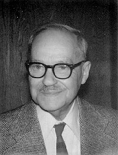
\includegraphics{figures/jerzyneyman.png}
\caption{Jerzy Neyman}
\end{figure}

\begin{center}\rule{0.5\linewidth}{\linethickness}\end{center}

\subsection{Confidence interval}\label{conf-interval}

The upper and lower bounds for the population means that are plausible
constitute an interval estimate of the parameter. This interval is
linked to a probability, for instance, 95\%.

It is very important that we understand that this is NOT the probability
that the parameter has a particular value, or that it falls within the
interval. The parameter is \emph{not} a random variable because it is
not affected by the random sample that we draw. In our example, it will
be clear that the sample that we draw does not and cannot change the
average weight of all candies.

The parameter has one value, which is either within or outside the
interval that we have constructed. We just don't know. But we do know
that our sample is more likely for population values within the
interval.

We use the term \emph{confidence} instead of probability when we use
this interval to estimate a parameter. The interval is called a
\emph{confidence interval} and we usually add the confidence level, for
instance, the 95\% confidence interval (abbreviated: 95\%CI). We are
95\% confident that the parameter falls within the 95\% confidence
interval. If the 95\% confidence interval for average candy weight
ranges from 2.4 to 3.2 gram, we write in our report:

\begin{quote}
We are 95\% confident that average candy weight in the population is
between 2.4 and 3.2 gram.
\end{quote}

\begin{figure}[H]
\href{http://82.196.4.233:3838/apps/95ci-simul/}{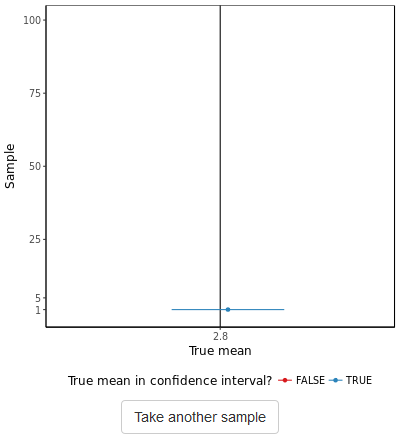
\includegraphics[width=420px]{GentleIntro_files/figure-latex/95ci-simul-1} }\caption{How often does a confidence interval include the true population value?}\label{fig:95ci-simul}
\end{figure}

Figure \ref{fig:95ci-simul} shows a 95\% confidence interval for average
candy weight in the population based on a sample of candies. The
vertical line indicates the true average candy weight in the population.

\begin{enumerate}
\def\labelenumi{\arabic{enumi}.}
\tightlist
\item
  Does the (first) confidence interval include the true average candy
  weight in the population?
\end{enumerate}

\begin{Shaded}
\begin{Highlighting}[]
\OperatorTok{*}\StringTok{ }\NormalTok{The first confidence interval }\KeywordTok{may}\NormalTok{ (blue) or may }\KeywordTok{not}\NormalTok{ (red) include the true}
\NormalTok{population }\KeywordTok{mean}\NormalTok{ (}\FloatTok{2.8}\NormalTok{).}
\OperatorTok{*}\StringTok{ }\NormalTok{The sample mean can be close enough to the true population mean }\ControlFlowTok{for}\NormalTok{ the}
\NormalTok{confidence interval to include the true population mean. But it can also be too}
\NormalTok{far from the true population mean.}
\OperatorTok{*}\StringTok{ }\NormalTok{A confidence interval, however, is much more likely to include the true}
\NormalTok{population mean than not.}
\end{Highlighting}
\end{Shaded}

\begin{enumerate}
\def\labelenumi{\arabic{enumi}.}
\setcounter{enumi}{1}
\tightlist
\item
  Why is the point estimate (dot) exactly in the middle of each
  confidence interval?
\end{enumerate}

\begin{Shaded}
\begin{Highlighting}[]
\OperatorTok{*}\StringTok{ }\NormalTok{In the preceding section, the limits of a confidence interval have been}
\NormalTok{calculated as the sample mean plus or minus the standard error times the}
\NormalTok{critical value. Because the upper limit of the confidence interval is exactly}
\NormalTok{as far away from the sample mean as the lower }\KeywordTok{limit}\NormalTok{ (namely, the standard}
\NormalTok{error times the critical value), the sample mean must be exactly }\ControlFlowTok{in}\NormalTok{ the middle}
\NormalTok{of the confidence interval.}
\end{Highlighting}
\end{Shaded}

\begin{enumerate}
\def\labelenumi{\arabic{enumi}.}
\setcounter{enumi}{2}
\tightlist
\item
  If you would draw a hundred random samples from the same population
  and calculate the 95\% confidence interval for the mean of each
  sample, how many confidence intervals will contain the true population
  mean? Press the \textbf{New Sample} button until there are one hundred
  confidence intervals. Does your expectation come true? If not, why
  not?
\end{enumerate}

\begin{Shaded}
\begin{Highlighting}[]
\OperatorTok{*}\StringTok{ }\NormalTok{The confidence level is the probability that our confidence interval includes}
\NormalTok{the true population value. If the confidence level is }\DecValTok{95}\NormalTok{%, the probability that}
\NormalTok{a confidence interval includes the true population value is .}\DecValTok{95}\NormalTok{, so we expect}
\NormalTok{that }\DecValTok{95}\NormalTok{ out of }\DecValTok{100}\NormalTok{ confidence intervals include the population mean.}
\OperatorTok{*}\StringTok{ }\NormalTok{With probabilities, the expected value is only certain to be found }\ControlFlowTok{in}\NormalTok{ an}
\NormalTok{infinitively large number of }\KeywordTok{draws}\NormalTok{ (samples). One hundred samples are quite few}
\ControlFlowTok{in}\NormalTok{ the light of infinity, so the number of samples including the true}
\NormalTok{population value may well be smaller or larger than }\DecValTok{95}\NormalTok{.}
\OperatorTok{*}\StringTok{ }\NormalTok{This is easier to see }\ControlFlowTok{if}\NormalTok{ we focus on the number of red confidence intervals}
\NormalTok{that do not include the true population value. This number is usually}
\NormalTok{(slightly) larger or smaller than five.}
\end{Highlighting}
\end{Shaded}

The more precise meaning of a confidence interval is rather complicated.
If we draw a very large number of samples from the same population, 95\%
of the sample means would differ less from the population mean than the
critical value times the standard error. This is just the definition of
critical value.

Because the critical value times the standard error also defines the
width of the confidence interval, we can reverse the statement. The
population mean would be within the 95\% confidence interval of 95\% of
all sample means. In other words, if we construct the 95\% confidence
interval for each sample mean, 95\% of all samples will have confidence
intervals that contain the true population mean.

Our confidence interval is a random variable because it depends on the
sample that we draw. After all, we construct the interval around the
sample statistic outcome, for instance, average candy weight in our
sample (the point estimate), which may change from sample to sample. So
we may say that the confidence level is the \emph{probability that our
confidence interval includes the true population value}. But we avoid
this interpretation because it is easily misread as the probability that
the true population value is in the interval. The latter reading is
wrong from the perspective that the population value is not a random
variable, so it does not have a probability.

Unfortunately, we have no clue whether or not our single sample belongs
to the 95 per cent of `lucky' samples with confidence intervals
containing the true population value. We can only hope and be confident
that this is the case.

\subsection{Confidence intervals with
bootstrapping}\label{bootstrap-confidenceinterval}

If we approximate the sampling distribution with a theoretical
probability distribution such as the normal (\emph{z}) or \emph{t}
distribution, critical values and the standard error are used to
calculate the confidence interval (see Section \ref{imag-pop-values}).

There are theoretical probability distributions that do not work with a
standard error, such as the \emph{F} distribution or chi-squared
distribution. If we use those distributions to approximate the sampling
distribution of a continuous sample statistic, for instance, the
quotient of two variances, we must use bootstrapping to obtain a
confidence interval.

As you probably remember from Section \ref{boot-approx}, we simulate an
entire sampling distribution if we bootstrap a statistic, for instance
the median candy weight in a sample bag. This simulated sampling
distribution can be used to estimate the standard error, which is by
definition the standard deviation of the sampling distribution. This
standard error can then be combined with critical values to calculate
the confidence interval.

As an alternative, we can just take the values separating the bottom
2.5\% and the top 2.5\% of all samples in the bootstrapped sampling
distribution as the lower and upper limits of the 95\% confidence
interval. This is known as the \emph{percentile approach}.

It is also possible to construct the entire sampling distribution in
exact approaches to the sampling distribution. Both the standard error
and percentiles can be used to create confidence intervals. This can be
very demanding in terms of computer time, so exact approaches to the
sampling distribution usually only report p values, not confidence
intervals.

\section{Confidence Intervals in SPSS}\label{SPSS-CI}

\subsection{Instruction}\label{instruction}

\begin{figure}[H]
\href{https://www.youtube.com/embed/7e1gCCKYcW4}{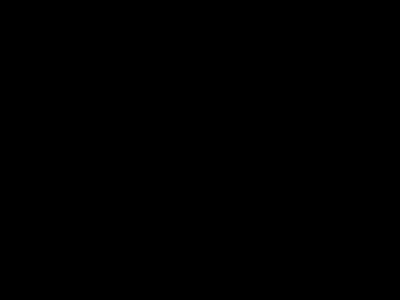
\includegraphics[width=320px]{GentleIntro_files/figure-latex/SPSSconflevel-1} }\caption{Setting the confidence level in SPSS.}\label{fig:SPSSconflevel}
\end{figure}

\subsection{Exercises}\label{exercises-2}

\begin{enumerate}
\def\labelenumi{\arabic{enumi}.}
\item
  Download the data set
  \href{http://82.196.4.233:3838/data/candies.sav}{candies.sav} and use
  SPSS to calculate the 95\% and 99\% confidence intervals of average
  candy weight.

  Hint: Use the \emph{Analyze \textgreater{} Compare Means
  \textgreater{} One-Sample T Test} command and leave the test value at
  zero.

  Interpret the results and explain why the 99\% confidence interval is
  wider than the 95\% confidence interval.
\end{enumerate}

\begin{Shaded}
\begin{Highlighting}[]
\NormalTok{SPSS syntax}\OperatorTok{:}\StringTok{  }
\StringTok{  }
\ErrorTok{*}\StringTok{ }\NormalTok{Check data.  }
\NormalTok{FREQUENCIES VARIABLES=weight  }
  \OperatorTok{/}\NormalTok{FORMAT=NOTABLE  }
  \OperatorTok{/}\NormalTok{HISTOGRAM NORMAL  }
  \OperatorTok{/}\NormalTok{ORDER=ANALYSIS.  }
\OperatorTok{*}\StringTok{ }\DecValTok{95}\NormalTok{% CI.  }
\NormalTok{T}\OperatorTok{-}\NormalTok{TEST  }
  \OperatorTok{/}\NormalTok{TESTVAL=}\DecValTok{0}  
  \OperatorTok{/}\NormalTok{MISSING=ANALYSIS  }
  \OperatorTok{/}\NormalTok{VARIABLES=weight  }
  \OperatorTok{/}\NormalTok{CRITERIA=}\KeywordTok{CI}\NormalTok{(.}\DecValTok{95}\NormalTok{).  }
\OperatorTok{*}\StringTok{ }\DecValTok{99}\NormalTok{% CI.  }
\NormalTok{T}\OperatorTok{-}\NormalTok{TEST  }
  \OperatorTok{/}\NormalTok{TESTVAL=}\DecValTok{0}  
  \OperatorTok{/}\NormalTok{MISSING=ANALYSIS  }
  \OperatorTok{/}\NormalTok{VARIABLES=weight  }
  \OperatorTok{/}\NormalTok{CRITERIA=}\KeywordTok{CI}\NormalTok{(.}\DecValTok{99}\NormalTok{).  }
  
\NormalTok{Check data}\OperatorTok{:}\StringTok{  }
\StringTok{  }
\NormalTok{There are no impossible values on variable weight.  }
  
\NormalTok{Check assumptions}\OperatorTok{:}\StringTok{  }
\StringTok{  }
\NormalTok{This is a t test, so sample size should be over }\DecValTok{30}\NormalTok{ or the variable should be}
\NormalTok{normally distributed }\ControlFlowTok{in}\NormalTok{ the population. The size of this }\KeywordTok{sample}\NormalTok{ (}\DataTypeTok{N =} \DecValTok{50}\NormalTok{) is}
\NormalTok{well over }\DecValTok{30}\NormalTok{, so we need not care about the normal distribution of candy}
\NormalTok{weight }\ControlFlowTok{in}\NormalTok{ the population.}
  
\NormalTok{Interpret the results}\OperatorTok{:}\StringTok{  }
\StringTok{  }
\NormalTok{Average weight of candies }\ControlFlowTok{in}\NormalTok{ the population is between }\FloatTok{2.79}\NormalTok{ and   }
\FloatTok{2.88}\NormalTok{ gram with }\DecValTok{95}\NormalTok{% confidence and between }\FloatTok{2.77}\NormalTok{ and }\FloatTok{2.90}\NormalTok{ gram  }
\NormalTok{with }\DecValTok{99}\NormalTok{% confidence.  }
\NormalTok{If we want to be more confident, we must allow }\ControlFlowTok{for}\NormalTok{ a broader  }
\NormalTok{range of values, so the confidence interval is wider.  }
\end{Highlighting}
\end{Shaded}

\begin{enumerate}
\def\labelenumi{\arabic{enumi}.}
\setcounter{enumi}{1}
\item
  Let SPSS calculate the 95\% confidence interval for median candy
  weight. Interpret the result. The data are in ``candies.sav''.

  Remember the SPSS exercises in Section \ref{boot-spss}.
\end{enumerate}

\begin{Shaded}
\begin{Highlighting}[]
\NormalTok{SPSS syntax}\OperatorTok{:}\StringTok{  }
\StringTok{  }
\ErrorTok{*}\StringTok{ }\NormalTok{Check data.  }
\NormalTok{FREQUENCIES VARIABLES=weight  }
  \OperatorTok{/}\NormalTok{ORDER=ANALYSIS.  }
\OperatorTok{*}\StringTok{ }\NormalTok{Bootstrap on median candy weight.  }
\NormalTok{BOOTSTRAP  }
  \OperatorTok{/}\NormalTok{SAMPLING METHOD=SIMPLE  }
  \OperatorTok{/}\NormalTok{VARIABLES INPUT=weight   }
  \OperatorTok{/}\NormalTok{CRITERIA CILEVEL=}\DecValTok{95}\NormalTok{ CITYPE=BCA  NSAMPLES=}\DecValTok{5000}  
  \OperatorTok{/}\NormalTok{MISSING USERMISSING=EXCLUDE.  }
\NormalTok{FREQUENCIES VARIABLES=weight  }
  \OperatorTok{/}\NormalTok{FORMAT=NOTABLE  }
  \OperatorTok{/}\NormalTok{STATISTICS=MEDIAN  }
  \OperatorTok{/}\NormalTok{ORDER=ANALYSIS.  }
  
\NormalTok{Check data}\OperatorTok{:}\StringTok{  }
\StringTok{    }
\NormalTok{There are no impossible values on the weight variable.  }
  
\NormalTok{Check assumptions}\OperatorTok{:}\StringTok{  }
\StringTok{    }
\NormalTok{The measurement level of variable weight is OK.  }
      
\NormalTok{Interpret the results}\OperatorTok{:}\StringTok{   }
\StringTok{  }
\NormalTok{Median candy weight }\ControlFlowTok{in}\NormalTok{ the sample is }\FloatTok{2.81}\NormalTok{ gram. With   }
\DecValTok{95}\NormalTok{% confidence, we expect median candy weight to be   }
\NormalTok{between }\FloatTok{2.77}\NormalTok{ and }\FloatTok{2.92}\NormalTok{ grams }\ControlFlowTok{in}\NormalTok{ the population of all candies. }
\NormalTok{The }\DecValTok{95}\NormalTok{% interval borders can be slightly different because}
\NormalTok{bootstrapping takes random samples.}
\end{Highlighting}
\end{Shaded}

\begin{enumerate}
\def\labelenumi{\arabic{enumi}.}
\setcounter{enumi}{2}
\item
  Use SPSS to determine the 95\% confidence interval for a
  paired-samples t test on candy colour fading under sunlight (variables
  colour\_pre and colour\_post in ``candies.sav''). In your
  interpretation of the confidence interval, clarify the meaning of the
  statistic for which the confidence interval was calculated.

  The paired-samples t test is available in SPSS under \emph{Analyze
  \textgreater{} Compare Means}.
\end{enumerate}

\begin{Shaded}
\begin{Highlighting}[]
\NormalTok{SPSS syntax}\OperatorTok{:}\StringTok{  }
\StringTok{  }
\ErrorTok{*}\StringTok{ }\NormalTok{Check data.  }
\NormalTok{FREQUENCIES VARIABLES=colour_pre colour_post  }
  \OperatorTok{/}\NormalTok{FORMAT=NOTABLE  }
  \OperatorTok{/}\NormalTok{HISTOGRAM NORMAL  }
  \OperatorTok{/}\NormalTok{ORDER=ANALYSIS.  }
\OperatorTok{*}\StringTok{ }\NormalTok{Paired}\OperatorTok{-}\NormalTok{samples t test.  }
\NormalTok{T}\OperatorTok{-}\NormalTok{TEST PAIRS=colour_pre WITH }\KeywordTok{colour_post}\NormalTok{ (PAIRED)  }
  \OperatorTok{/}\NormalTok{CRITERIA=}\KeywordTok{CI}\NormalTok{(.}\DecValTok{9500}\NormalTok{)  }
  \OperatorTok{/}\NormalTok{MISSING=ANALYSIS.  }
  
\NormalTok{Check data}\OperatorTok{:}\StringTok{  }
\StringTok{  }
\NormalTok{There are no impossible values on variable weight.  }
  
\NormalTok{Check assumptions}\OperatorTok{:}\StringTok{  }
\StringTok{  }
\NormalTok{Sample }\KeywordTok{size}\NormalTok{ (}\DataTypeTok{N =} \DecValTok{50}\NormalTok{) is well over }\DecValTok{30}\NormalTok{, so we need not care about  }
\NormalTok{the normal distribution of candy weight }\ControlFlowTok{in}\NormalTok{ the population.  }
  
\NormalTok{Interpret the results}\OperatorTok{:}\StringTok{  }
\StringTok{  }
\NormalTok{Candy colourfulness fades under sunlight by }\FloatTok{1.88}\NormalTok{ (or between   }
\FloatTok{1.59}\NormalTok{ to }\FloatTok{2.17}\NormalTok{) points }\ControlFlowTok{in}\NormalTok{ the data. This change is statistically   }
\NormalTok{significant, }\KeywordTok{t}\NormalTok{ (}\DecValTok{49}\NormalTok{) =}\StringTok{ }\FloatTok{12.86}\NormalTok{, p }\OperatorTok{<}\StringTok{ }\DecValTok{001}\NormalTok{, }\DecValTok{95}\NormalTok{%CI[}\FloatTok{1.59}\NormalTok{; }\FloatTok{2.17}\NormalTok{].  }
\end{Highlighting}
\end{Shaded}

\begin{enumerate}
\def\labelenumi{\arabic{enumi}.}
\setcounter{enumi}{3}
\item
  Use SPSS to determine if candy colourfulness after exposure to
  sunlight (colour\_post) depends on candy weight and candy sweetness.
  Interpret the 95\% confidence intervals for both effects.

  Hint: Use regression analysis, which is available under \emph{Analyze
  \textgreater{} Regression \textgreater{} Linear} in SPSS.
\end{enumerate}

\begin{Shaded}
\begin{Highlighting}[]
\NormalTok{SPSS syntax}\OperatorTok{:}\StringTok{  }
\StringTok{  }
\ErrorTok{*}\StringTok{ }\NormalTok{Check data}\OperatorTok{:}\StringTok{ }\NormalTok{Assumption checks }\ControlFlowTok{in}\NormalTok{ Chapter }\DecValTok{8}\NormalTok{.  }
\OperatorTok{*}\StringTok{ }\NormalTok{Check }\ControlFlowTok{for}\NormalTok{ impossible values.  }
\NormalTok{FREQUENCIES VARIABLES=weight sweetness colour_post  }
  \OperatorTok{/}\NormalTok{ORDER=ANALYSIS.  }
\OperatorTok{*}\StringTok{ }\NormalTok{Regression of colour_post on weight and sweetness.   }
\NormalTok{REGRESSION  }
  \OperatorTok{/}\NormalTok{MISSING LISTWISE  }
  \OperatorTok{/}\NormalTok{STATISTICS COEFF OUTS }\KeywordTok{CI}\NormalTok{(}\DecValTok{95}\NormalTok{) R ANOVA  }
  \OperatorTok{/}\NormalTok{CRITERIA=}\KeywordTok{PIN}\NormalTok{(.}\DecValTok{05}\NormalTok{) }\KeywordTok{POUT}\NormalTok{(.}\DecValTok{10}\NormalTok{)  }
  \OperatorTok{/}\NormalTok{NOORIGIN   }
  \OperatorTok{/}\NormalTok{DEPENDENT colour_post  }
  \OperatorTok{/}\NormalTok{METHOD=ENTER weight sweetness.  }
  
\NormalTok{Check data}\OperatorTok{:}\StringTok{   }
\StringTok{  }
\NormalTok{There are no impossible values on the variables.  }
  
\NormalTok{Check assumptions}\OperatorTok{:}\StringTok{  }
\StringTok{  }
\NormalTok{Assumptions are presented }\KeywordTok{later}\NormalTok{ (Chapter }\DecValTok{8}\NormalTok{).  }
  
\NormalTok{Interpret the results}\OperatorTok{:}\StringTok{  }
\StringTok{  }
\NormalTok{We are }\DecValTok{95}\NormalTok{ per cent confident that average candy  }
\NormalTok{colourfulness decreases by }\FloatTok{0.19}\NormalTok{ to }\FloatTok{0.46} \ControlFlowTok{for}  
\NormalTok{each additional unit of sweetness }\ControlFlowTok{in}\NormalTok{ the  }
\NormalTok{population.  }
\NormalTok{We are not confident about the direction of the  }
\NormalTok{effect of candy weight on colourfulness. This  }
\NormalTok{effect can be }\KeywordTok{negative}\NormalTok{ (up to a }\FloatTok{1.15}\NormalTok{ decrease }\ControlFlowTok{for}  
\NormalTok{each additional candy weight gram with }\DecValTok{95}\NormalTok{% confidence)}
\NormalTok{or }\KeywordTok{positive}\NormalTok{ (up to a }\FloatTok{2.28}\NormalTok{ increase }\ControlFlowTok{for}\NormalTok{ each additional}
\NormalTok{candy weight gram with }\DecValTok{95}\NormalTok{% confidence).  }
\end{Highlighting}
\end{Shaded}

\section{Test Your Understanding}\label{test-your-understanding-2}

\begin{figure}[H]
\href{http://82.196.4.233:3838/apps/estimation/}{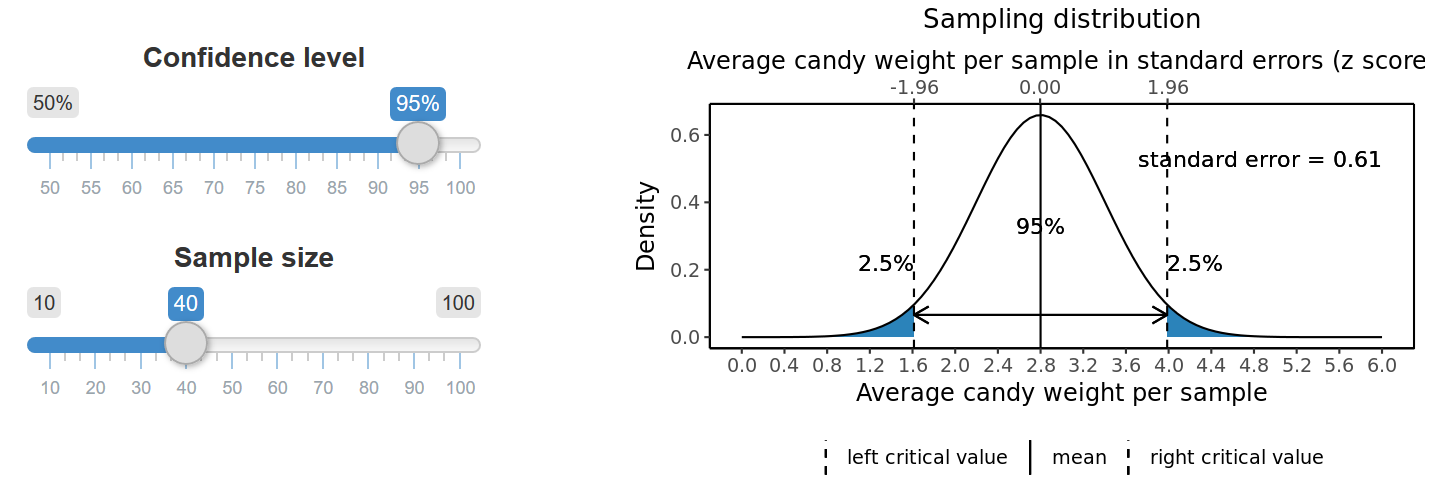
\includegraphics[width=420px]{GentleIntro_files/figure-latex/estimation-1} }\caption{Point and interval estimates, confidence intervals.}\label{fig:estimation}
\end{figure}

Figure \ref{fig:estimation} shows the sampling distribution of average
candy weight in a sample bag, which is a normal distribution.

\begin{enumerate}
\def\labelenumi{\arabic{enumi}.}
\tightlist
\item
  What is the most likely estimate for average candy weight in the
  population?
\end{enumerate}

\begin{Shaded}
\begin{Highlighting}[]
\OperatorTok{*}\StringTok{ }\NormalTok{The average of a distribution of sample means is the expected value or}
\NormalTok{expectation of the population }\KeywordTok{mean}\NormalTok{ (because a sample mean is an unbiased}
\NormalTok{estimate of a population mean).}
\OperatorTok{*}\StringTok{ }\NormalTok{The mean of average candy weight over all samples is }\FloatTok{2.8}\NormalTok{ gram }\ControlFlowTok{in}\NormalTok{ this}
\NormalTok{example. This is our best }\KeywordTok{guess}\NormalTok{ (point estimate) }\ControlFlowTok{for}\NormalTok{ average candy weight }\ControlFlowTok{in}
\NormalTok{the population.}
\OperatorTok{*}\StringTok{ }\NormalTok{The }\KeywordTok{density}\NormalTok{ (not the probability}\OperatorTok{!}\NormalTok{) of the sampling distribution is at its}
\NormalTok{maximum at }\FloatTok{2.8}\NormalTok{ gram.}
\end{Highlighting}
\end{Shaded}

\begin{enumerate}
\def\labelenumi{\arabic{enumi}.}
\setcounter{enumi}{1}
\tightlist
\item
  The percentage in between the two vertical lines can be interpreted as
  a probability. A probability of what?
\end{enumerate}

\begin{Shaded}
\begin{Highlighting}[]
\OperatorTok{*}\StringTok{ }\NormalTok{The probability to draw a }\KeywordTok{sample}\NormalTok{ (bag) with a sample }\KeywordTok{mean}\NormalTok{ (average candy}
\NormalTok{weight) between the value of the }\KeywordTok{left}\NormalTok{ (lower) limit and the }\KeywordTok{right}\NormalTok{ (upper)}
\NormalTok{limit.}
\end{Highlighting}
\end{Shaded}

\begin{enumerate}
\def\labelenumi{\arabic{enumi}.}
\setcounter{enumi}{2}
\tightlist
\item
  The double arrow represents an interval of sample means, in this
  example, average candy weight. What happens if you change the
  confidence level? Explain why this makes sense.
\end{enumerate}

\begin{Shaded}
\begin{Highlighting}[]
\OperatorTok{*}\StringTok{ }\NormalTok{Raising the confidence level increases the width of the interval because it}
\NormalTok{increases the area under the curve between the interval limits.}
\OperatorTok{*}\StringTok{ }\NormalTok{This makes sense because the confidence level is the probability of drawing}
\NormalTok{a sample with a }\KeywordTok{mean}\NormalTok{ (sample statistic value) within the interval.}
\OperatorTok{*}\StringTok{ }\NormalTok{If we want to have a higher probability, we must be more inclusive, that is,}
\NormalTok{we must allow }\ControlFlowTok{for}\NormalTok{ a greater range of sample means.}
\end{Highlighting}
\end{Shaded}

\begin{enumerate}
\def\labelenumi{\arabic{enumi}.}
\setcounter{enumi}{3}
\tightlist
\item
  What happens to the graph if you change sample size?
\end{enumerate}

\begin{Shaded}
\begin{Highlighting}[]
\OperatorTok{*}\StringTok{ }\NormalTok{A larger sample size makes the sampling distribution more peaked, so the}
\NormalTok{interval containing the middle }\DecValTok{95}\NormalTok{% of all samples becomes narrower.}
\OperatorTok{*}\StringTok{ }\NormalTok{We have to expect less variation }\ControlFlowTok{in}\NormalTok{ sample means, so we have a more precise}
\NormalTok{estimate of the sample mean that we are very }\KeywordTok{likely}\NormalTok{ (}\DecValTok{95}\NormalTok{% probability) to draw.}
\end{Highlighting}
\end{Shaded}

\begin{enumerate}
\def\labelenumi{\arabic{enumi}.}
\setcounter{enumi}{4}
\tightlist
\item
  What happens to the standard error if you change sample size? How are
  sample size and standard error linked? What characteristic of the
  sampling distribution is expressed by the standard error?
\end{enumerate}

\begin{Shaded}
\begin{Highlighting}[]
\OperatorTok{*}\StringTok{ }\NormalTok{Increasing sample size decreases the standard error, so the two are}
\NormalTok{negatively correlated. A larger sample size creates a more peaked}
\NormalTok{distribution, which indicates lower }\KeywordTok{variation}\NormalTok{ (scores are closer to the mean).}
\NormalTok{This makes sense}\OperatorTok{:}\StringTok{ }\NormalTok{A larger sample contains more information, so its mean}
\KeywordTok{should}\NormalTok{ (on average) be closer to the true population }\KeywordTok{mean}\NormalTok{ (hence to the mean}
\NormalTok{of the sampling distribution).}
\OperatorTok{*}\StringTok{ }\NormalTok{The standard error expresses the variation }\ControlFlowTok{in}\NormalTok{ the sampling distribution.}
\NormalTok{Actually, the standard error is just the standard deviation of the sampling}
\NormalTok{distribution.}
\end{Highlighting}
\end{Shaded}

\begin{enumerate}
\def\labelenumi{\arabic{enumi}.}
\setcounter{enumi}{5}
\tightlist
\item
  The values of the interval limits---average candy weights in this
  example---on the scale in standard errors are called critical values.
  What happens to the critical values if you change sample size?
\end{enumerate}

\begin{Shaded}
\begin{Highlighting}[]
\OperatorTok{*}\StringTok{ }\NormalTok{Nothing changes. Critical values are fixed values }\ControlFlowTok{in}\NormalTok{ terms of standard}
\NormalTok{errors }\ControlFlowTok{if}\NormalTok{ the confidence }\KeywordTok{level}\NormalTok{ (and the degrees of freedom that we will}
\NormalTok{discuss later) do not change.}
\OperatorTok{*}\StringTok{ }\NormalTok{If this was a t distribution, the critical values would slightly decrease }
\NormalTok{with larger sample size but this change is too small to be of practical }
\NormalTok{relevance, so it is ignored }\ControlFlowTok{in}\NormalTok{ this web book.}
\end{Highlighting}
\end{Shaded}

\begin{enumerate}
\def\labelenumi{\arabic{enumi}.}
\setcounter{enumi}{6}
\tightlist
\item
  What happens to the critical values if you change the confidence
  level?
\end{enumerate}

\begin{Shaded}
\begin{Highlighting}[]
\OperatorTok{*}\StringTok{ }\NormalTok{Higher confidence levels yield more extreme critical values because }
\NormalTok{the interval must cover a larger proportion of all possible samples.}
\end{Highlighting}
\end{Shaded}

\begin{enumerate}
\def\labelenumi{\arabic{enumi}.}
\setcounter{enumi}{7}
\tightlist
\item
  If the centre of the sampling distribution in Figure
  \ref{fig:estimation} (2.8) is the average candy weight in the sample
  instead of the population average, the interval marked by the arrows
  is called a \emph{confidence interval}. In this example, a confidence
  interval for what? And what is the value of the point estimate here?
\end{enumerate}

\begin{Shaded}
\begin{Highlighting}[]
\OperatorTok{*}\StringTok{ }\NormalTok{A confidence interval always belongs to a population }\KeywordTok{statistic}\NormalTok{ (parameter).}
\NormalTok{In this example, we use the sample mean to estimate the population mean, so}
\NormalTok{the confidence interval refers to average candy weight }\ControlFlowTok{in}\NormalTok{ the population. The}
\NormalTok{point estimate, which gives a single number instead of an interval, would be}
\FloatTok{2.8}\NormalTok{ grams here.}
\end{Highlighting}
\end{Shaded}

\section{Take-Home Points}\label{take-home-points-2}

\begin{itemize}
\item
  If a sample statistic is an unbiased estimator, we can use it as a
  point estimate for the value of the statistic in the population.
\item
  A point estimate may come close to the population value but it is
  almost certainly not correct.
\item
  A 95\% confidence interval is an interval estimate of the population
  value. We are 95\% confident that the population value lies within
  this interval. Note that confidence is not a probability!
\item
  A larger sample or a lower confidence level yields a narrower, that
  is, a more precise confidence interval.
\item
  A larger sample yields a smaller standard error, which yields a more
  precise confidence interval because the limits of a 95\% confidence
  interval fall one standard error times the critical value below and
  above the value of the sample statistic.
\end{itemize}

\chapter{Testing a Null Hypothesis: Am I Right or Am I
Wrong?}\label{hypothesis}

\begin{quote}
Key concepts: research hypothesis, statistical null and alternative
hypothesis, nil hypothesis, test statistic, p value, significance level
(Type I error rate), Type I error, inflated Type I error, capitalization
on chance, one-sided and two-sided tests and tests to which this
distinction does not apply, rejection region.
\end{quote}

\subsection*{Summary}\label{summary-3}
\addcontentsline{toc}{subsection}{Summary}

\begin{quote}
Is my sample probable if the null hypothesis is true?
\end{quote}

In the preceding chapter, we have learned that a confidence interval
contains the population values that are plausible, given the sample that
we have drawn. In the current chapter, we narrow this down to the
question whether the expectation of the researcher about the population
is plausible.

The expectation is usually called a (research) hypothesis and it must be
translated into statistical hypotheses about a population value
(parameter): a null hypothesis and an alternative hypothesis.

We test a null hypothesis in the following way. We construct a sampling
distribution in one of the ways we have learned in Chapter
\ref{probmodels} using the value specified in the null hypothesis as the
hypothetical population value. In other words, we act as if the null
hypothesis is true.

Then, we calculate the probability of drawing a sample such as the one
we have drawn or a sample that differs even more from the hypothesized
population value. If this probability (p value) is very low, say, below
5\%, we reject the null hypothesis because our sample would be too
unlikely if the null hypothesis is true. In this case, the test is
statistically significant. The probability threshold that we use is
called the significance level of the test.

\section{A Binary Decision}\label{binarydecision}

The overall goal of statistical inference is to increase our knowledge
about a population, when we only have a random sample from that
population. In Chapter \ref{param-estim}, we estimated population values
that are plausible considering the sample that we have drawn. For
instance, we looked for all plausible average weights of candies in the
population using information about the weight of candies in our sample
bag. This is what we do when we estimate a population value.

Estimation is one of two types of statistical inference, the other being
null hypothesis testing. When we estimate a population value, we do not
use our previous knowledge about the world of candies or whatever other
subject we are investigating. We can be completely ignorant about the
phenomenon that we are investigating. This approach is not entirely in
line with the conceptualization of scientific progress as an
\emph{empirical cycle}, in which scientists develop theories about the
empirical world, test these theories against data collected from this
world, and improve their theories if they are contradicted by the data
(de Groot,
\protect\hyperlink{ref-deGrootMethodologyFoundationsInference1969}{1969}).

Hypothesis testing, however, is more in line with this conceptualization
of scientific progress. It requires the researcher to formulate an
expectation about the population, usually called a \emph{hypothesis}. If
the hypothesis is based on theory and previous research, the scientist
uses previous knowledge. As a next step, the researcher tests the
hypothesis against data collected for this purpose. If the data
contradict the hypothesis, the hypothesis is rejected and the researcher
has to improve the theory. If the data does not contradict the
hypothesis, it is not rejected and, for the time being, the researcher
does not have to change the theory.

Hypothesis testing, then, amounts to choosing one of two options: reject
or not reject the hypothesis. This is a binary decision between
believing that the population is as it is described in the null
hypothesis, or believing that it is not. This is quite a different
approach than estimating a confidence interval as a range of plausible
population values. Nevertheless, hypothesis testing and confidence
intervals are tightly related as we will see later on in this chapter
(Section \ref{null-ci0}).

\section{Statistical Tests}\label{statistical-tests}

A statistical test determines whether a statement about a population is
plausible given a sample that is drawn from this population. In essence,
a statistical test answers the question: Is the sample that we have
drawn sufficiently plausible if the statement about the population would
be true?

We need several ingredients to apply a statistical test:

\begin{enumerate}
\def\labelenumi{\arabic{enumi}.}
\item
  A statement about a population.
\item
  A sample from the population supplying information about the
  statement.
\item
  A criterion to decide when the statement is sufficiently plausible.
\item
  A probability for the statement showing how plausible the statement
  is.
\end{enumerate}

This section discusses these four ingredients of a statistical test. The
statement about a population is the null hypothesis of the test (Section
\ref{nullhypothesis}). The sample must contain the variable or variables
addressed in the null hypothesis, so we discuss the sample in the
section on the null hypothesis. We select a significance level, usually
five per cent, as criterion to decide whether the null hypothesis is
sufficiently plausible or not. In the latter case, we reject the null
hypothesis. The values for which we reject the null hypothesis
constitute the rejection region of the test (Section \ref{sig-typeI}).
Finally, we let the computer calculate a probability (p value) for
drawing a sample that differs at least as much from the null hypothesis
as the sample that we have drawn. If this probability is smaller than
the selected significance level, the sample is in the rejection region,
so we must reject the null hypothesis (Section \ref{pvalue}). This
concludes the statistical test.

\subsection{The null hypothesis and the sample}\label{nullhypothesis}

The statement that a research wants to test is called a \emph{research
hypothesis}. It is a statement about the empirical world that can be
tested against data. Communication scientists, for instance, may
hypothesize that:

\begin{itemize}
\item
  a television station reaches half of all households in a country,
\item
  media literacy is below a particular standard (for instance, 5.5 on a
  10-point scale) among children,
\item
  opinions about immigrants are not equally polarized among young and
  old voters,
\item
  the celebrity endorsing a fundraising campaign makes a difference to
  adult's willingness to donate,
\item
  more exposure to brand advertisements increases brand awareness of
  consumers,
\item
  and so on.
\end{itemize}

These are statements about populations: all households in a country,
children, voters, adults, and consumers. As these examples illustrate,
research hypotheses seldom refer to statistics such as means,
proportions, variances, or correlations. Still, we need a statistic to
test a hypothesis. The researcher must translate the research hypothesis
into a new hypothesis that refers to a statistic in the population, for
example, the population mean. The new hypothesis is called a
\emph{statistical hypothesis}.

\begin{enumerate}
\def\labelenumi{\arabic{enumi}.}
\tightlist
\item
  Which statistics are addressed in the examples of research hypotheses
  above?
\end{enumerate}

\begin{Shaded}
\begin{Highlighting}[]
\OperatorTok{*}\StringTok{ }\NormalTok{A television station reaches half of all households }\ControlFlowTok{in}\NormalTok{ a country}\OperatorTok{:}\StringTok{ }\NormalTok{This}
\NormalTok{hypothesis is about a }\KeywordTok{proportion}\NormalTok{ (share)}\OperatorTok{:}\StringTok{ }\KeywordTok{half}\NormalTok{ (}\DecValTok{50}\NormalTok{%) of all households.}
\OperatorTok{*}\StringTok{ }\NormalTok{Media literacy is below }\FloatTok{5.5}\NormalTok{ (on a }\DecValTok{10}\OperatorTok{-}\NormalTok{point scale) among children}\OperatorTok{:}\StringTok{ }\NormalTok{This}
\NormalTok{hypothesis probably addresses a population mean, namely average media}
\NormalTok{literacy.}
\OperatorTok{*}\StringTok{ }\NormalTok{Opinions about immigrants are not equally polarized among young and old}
\NormalTok{voters}\OperatorTok{:}\StringTok{ }\NormalTok{It is not so easy to see, but this hypothesis is about variation }\ControlFlowTok{in}
\NormalTok{scores, namely the variance }\ControlFlowTok{in}\NormalTok{ opinion scores among young voters and the}
\NormalTok{variation among old voters.}
\OperatorTok{*}\StringTok{ }\NormalTok{The celebrity endorsing a fundraising campaign makes a difference to}
\NormalTok{willingness to donate}\OperatorTok{:}\StringTok{ }\NormalTok{People exposed to different endorsers are expected to}
\NormalTok{have }\KeywordTok{different}\NormalTok{ (levels of) willingness to donate. We are probably going to}
\NormalTok{compare the mean or median willingness across groups of people.}
\OperatorTok{*}\StringTok{ }\NormalTok{More exposure to brand advertisements increases brand awareness}\OperatorTok{:}\StringTok{ }\NormalTok{This}
\NormalTok{probably refers to a correlation or regression between brand advertisements}
\NormalTok{and brand awareness.}
\end{Highlighting}
\end{Shaded}

The most important statistical hypothesis is called the \emph{null
hypothesis} (\emph{H}\textsubscript{0}). \emph{The null hypothesis
specifies one value for a population statistic}. For example, it
hypothesizes that average media literacy in the population of children
equals 5.5 on a scale from one to ten. If 5.5 distinguishes between
sufficient and insufficient media literacy on a ten-point scale, it is
interesting to know whether average media literacy of children is just
sufficient or not.

We can test this statement about the population with a random sample of
children drawn from the population in which we measure their media
literacy. Once we have the measurements, we can calculate average media
literacy in the sample. We can compare the sample average to the
hypothesized average media literacy in the population. If they are not
too far apart, we conclude that the null hypothesis is plausible. If
they are too far apart, we don't think the null hypothesis is plausible
and we reject it.

\subsection{\texorpdfstring{Significance level (\(\alpha\)),
significance, rejection region, and Type I
error}{Significance level (\textbackslash{}alpha), significance, rejection region, and Type I error}}\label{sig-typeI}

How far apart must the sample statistic value and the hypothesized
population value be to conclude that the null hypothesis is not
plausible? The null hypothesis is supposed to be implausible if the
sample that we have drawn is among the samples that are very unlikely if
the null hypothesis is true. A commonly accepted threshold value is that
the sample is among the five per cent most unlikely samples. This
threshold is called the \emph{significance level} of the test. It is
often represented by the symbol \(\alpha\). If our sample is among the
five per cent most unlikely samples, we reject the null hypothesis and
we say that the test is \emph{statistically significant}.

We can construct a sampling distribution around the hypothesized
population value. Remember (Section \ref{expectedvalue}) that the
population value is the expected value of the sampling distribution,
that is, it's mean (if the estimator is unbiased). The sampling
distribution, then, is centered around the population value specified in
the null hypothesis. This sampling distribution tells us the
probabilities of all possible sample outcomes \emph{if the null
hypothesis is true}. It allows us to identify the most unlikely samples,
that is, the samples for which we reject the null hypothesis.

Note that we can construct a sampling distribution for the null
hypothesis only if the hypothesis specifies one value for the population
statistic. If we would have multiple population values in our null
hypothesis, for example, average media literacy is 5.5, 5.0, or 4.5 in
the population, we would have multiple sampling distributions: one for
each value. This is why the null hypothesis must specify a single value.

Let us assume that average media literacy is 3.9 in our sample.
According to our null hypothesis, the population average is 5.5. If
average media literacy of children in the population would really be
5.5, is our sample with 3.9 as average media literacy among the five per
cent most unlikely samples? We can use a hypothetical sampling
distribution with 5.5 as mean value to answer this question.

\begin{figure}[H]
\href{http://82.196.4.233:3838/apps/nullsampling/}{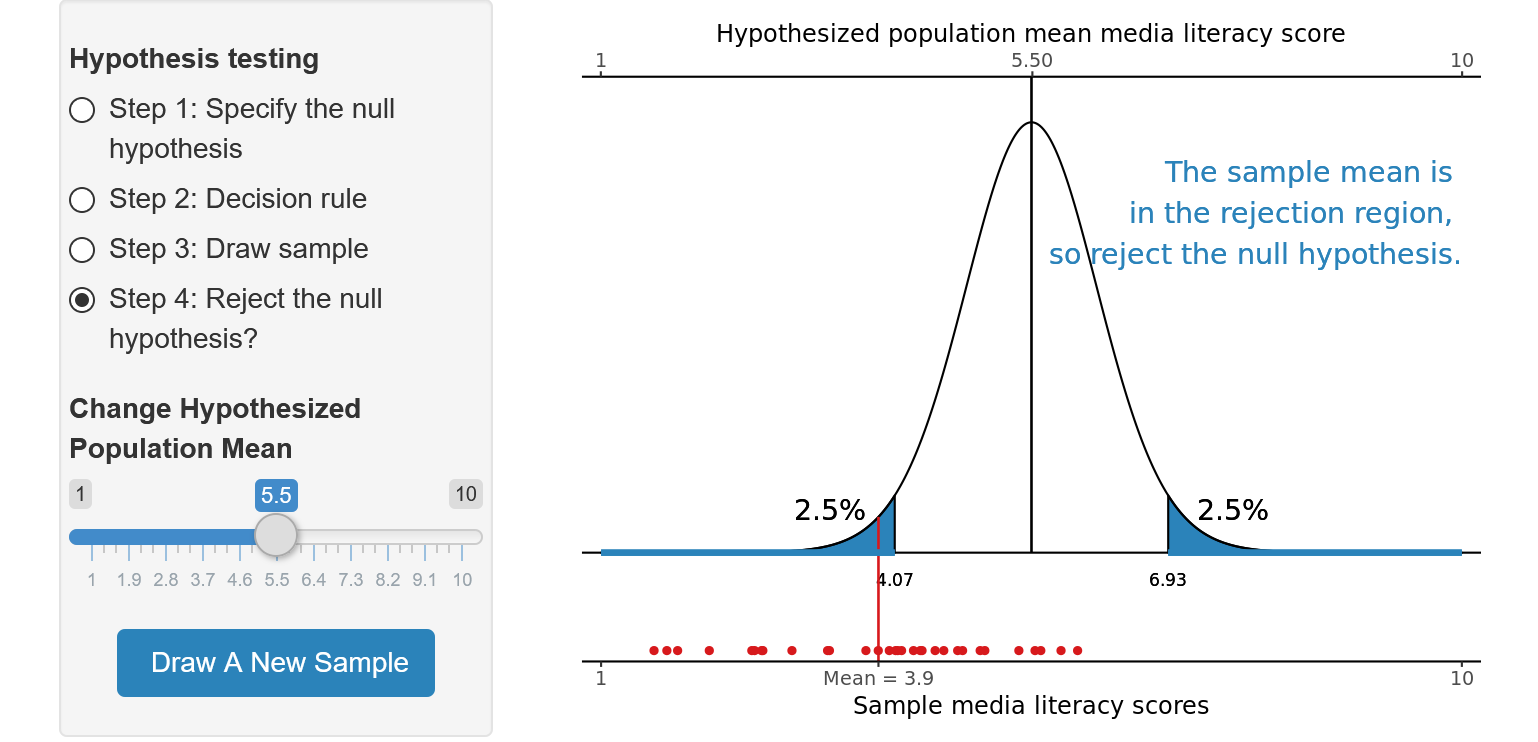
\includegraphics[width=420px]{GentleIntro_files/figure-latex/nullsampling-1} }\caption{Sampling distribution of average media literacy according to the null hypothesis.}\label{fig:nullsampling}
\end{figure}

\begin{enumerate}
\def\labelenumi{\arabic{enumi}.}
\tightlist
\item
  Figure \ref{fig:nullsampling} shows the hypothesized population mean,
  the associated sampling distribution, and the sample scores (red dots)
  with their mean. Formulate the null hypothesis represented by this
  figure.
\end{enumerate}

\begin{Shaded}
\begin{Highlighting}[]
\OperatorTok{*}\StringTok{ }\NormalTok{The null hypothesis}\OperatorTok{:}\StringTok{ }\NormalTok{In the population of children, average media literacy}
\NormalTok{is }\FloatTok{5.5}\NormalTok{.}
\OperatorTok{*}\StringTok{ }\NormalTok{Be sure to mention that the null hypothesis concerns a population.}
\OperatorTok{*}\StringTok{ }\NormalTok{This example is about average media literacy, so the null hypothesis}
\NormalTok{statistic is the average.}
\OperatorTok{*}\StringTok{ }\NormalTok{The }\KeywordTok{average}\NormalTok{ (middle) of the sampling distribution is }\FloatTok{5.5}\NormalTok{. This must be the}
\NormalTok{hypothesized population value }\KeywordTok{because}\NormalTok{ (the sample mean is an unbiased estimator}
\NormalTok{of the population mean, so) the population value is the average of the sampling}
\NormalTok{distribution.}
\end{Highlighting}
\end{Shaded}

\begin{enumerate}
\def\labelenumi{\arabic{enumi}.}
\setcounter{enumi}{1}
\tightlist
\item
  How can you create a sampling distribution for a null hypothesis that
  specifies 4.3 as selected value?
\end{enumerate}

\begin{Shaded}
\begin{Highlighting}[]
\OperatorTok{*}\StringTok{ }\NormalTok{Just change the hypothesized population mean with the slider.}
\end{Highlighting}
\end{Shaded}

\begin{enumerate}
\def\labelenumi{\arabic{enumi}.}
\setcounter{enumi}{2}
\tightlist
\item
  The significance level is five per cent here. Why is it marked by two
  blue tails?
\end{enumerate}

\begin{Shaded}
\begin{Highlighting}[]
\OperatorTok{*}\StringTok{ }\NormalTok{The significance level is a proportion or probability, so it is expressed by}
\NormalTok{a surface under }\KeywordTok{the}\NormalTok{ (probability density) curve.}
\OperatorTok{*}\StringTok{ }\NormalTok{The sample average can be too low, so half of the risk is situated }\ControlFlowTok{in}\NormalTok{ the}
\NormalTok{left tail, but it can also be too high, so the other half of the risk is}
\NormalTok{situated }\ControlFlowTok{in}\NormalTok{ the right tail.}
\end{Highlighting}
\end{Shaded}

\begin{enumerate}
\def\labelenumi{\arabic{enumi}.}
\setcounter{enumi}{3}
\tightlist
\item
  How low or high must the sample mean be to have a statistically
  significant test result?
\end{enumerate}

\begin{Shaded}
\begin{Highlighting}[]
\OperatorTok{*}\StringTok{ }\NormalTok{In the initial example, with average population media literacy hypothesized}
\NormalTok{to be }\FloatTok{5.5}\NormalTok{ and }\FloatTok{3.9}\NormalTok{ as the sample mean, sample means below }\FloatTok{4.07}\NormalTok{ or above }\FloatTok{6.93}
\NormalTok{are }\ControlFlowTok{in}\NormalTok{ the blue tails. They are statistically significantly different from the}
\NormalTok{hypothesized population value.}
\end{Highlighting}
\end{Shaded}

\begin{enumerate}
\def\labelenumi{\arabic{enumi}.}
\setcounter{enumi}{4}
\tightlist
\item
  Is it always possible to formulate a null hypothesis such that the
  sample mean is statistically significant? Take some new samples and
  change the value of the null hypothesis to check your answer.
\end{enumerate}

\begin{Shaded}
\begin{Highlighting}[]
\OperatorTok{*}\StringTok{ }\NormalTok{If the null hypothesis changes, the hypothesized population average, hence}
\NormalTok{the centre of the sampling distribution moves left or right. And so do the}
\NormalTok{blue tails that indicate statistically significant results.}
\OperatorTok{*}\StringTok{ }\NormalTok{Thus, it is always possible to find a hypothesized population value }\ControlFlowTok{for}
\NormalTok{which the sample mean ends up }\ControlFlowTok{in}\NormalTok{ a blue tail, so it is statistically}
\NormalTok{significant.}
\end{Highlighting}
\end{Shaded}

\begin{enumerate}
\def\labelenumi{\arabic{enumi}.}
\setcounter{enumi}{5}
\tightlist
\item
  What is special about a significance level of five per cent?
\end{enumerate}

\begin{Shaded}
\begin{Highlighting}[]
\NormalTok{Nothing is special about a significance level of five per cent. We could have}
\NormalTok{used any other cutoff value. It is just a convention to use this level.}
\end{Highlighting}
\end{Shaded}

The values for the sample statistic for which the test is statistically
significant constitute the \emph{rejection region} of the test. If the
sample statistic is in the rejection region, we reject the null
hypothesis. Note that the rejection region has two separate parts: a
part in the left tail and a part in the right tail of the sampling
distribution. Average media literacy can be too low to maintain the null
hypothesis that it is 5.5 in the population, but it can also be too
high. The threshold value of five per cent is divided into two halves of
2.5\% per cent; one for each tail.

If the sample statistic is in the rejection region, we have to reject
the null hypothesis. Those are the rules of the game. However, our
conclusion that the null hypothesis is wrong can be a mistake because
the null hypothesis may still be true. For example, average media
literacy is really 5.5 in the population, but we were so unfortunate to
draw a sample of children with very low media literacy scores. This
error is called a \emph{Type I error}: rejecting a hypothesis that is
actually true.

We don't know whether or when we make this error. We cannot entirely
avoid this error because samples can be very different from the
population from which they are drawn, as we learned in Chapter
\ref{samp-dist}. Thankfully, however, we know the probability that we
make this error. This probability is the significance level.

You should understand the exact meaning of probabilities here. A
significance level of .05 allows five per cent of all possible samples
to be so different from the population that we reject the null
hypothesis even if it is true.

In other words, if we draw a lot of samples and decide on the null
hypothesis for each sample, we would reject a true null hypothesis in
five per cent of our decisions. So we have a five per cent chance of
making a Type I error. We decide on that probability when we select the
confidence level of the test. We think that .05 is an acceptable
probability for making this type of error.

\subsection{p Value}\label{pvalue}

How do we know that the sample that we have drawn is among the five
percent most unlikely samples if the null hypothesis is true? In other
words, how do we know that our sample statistic outcome is in the
rejection region?

\begin{figure}[H]
\href{http://82.196.4.233:3838/apps/twosided/}{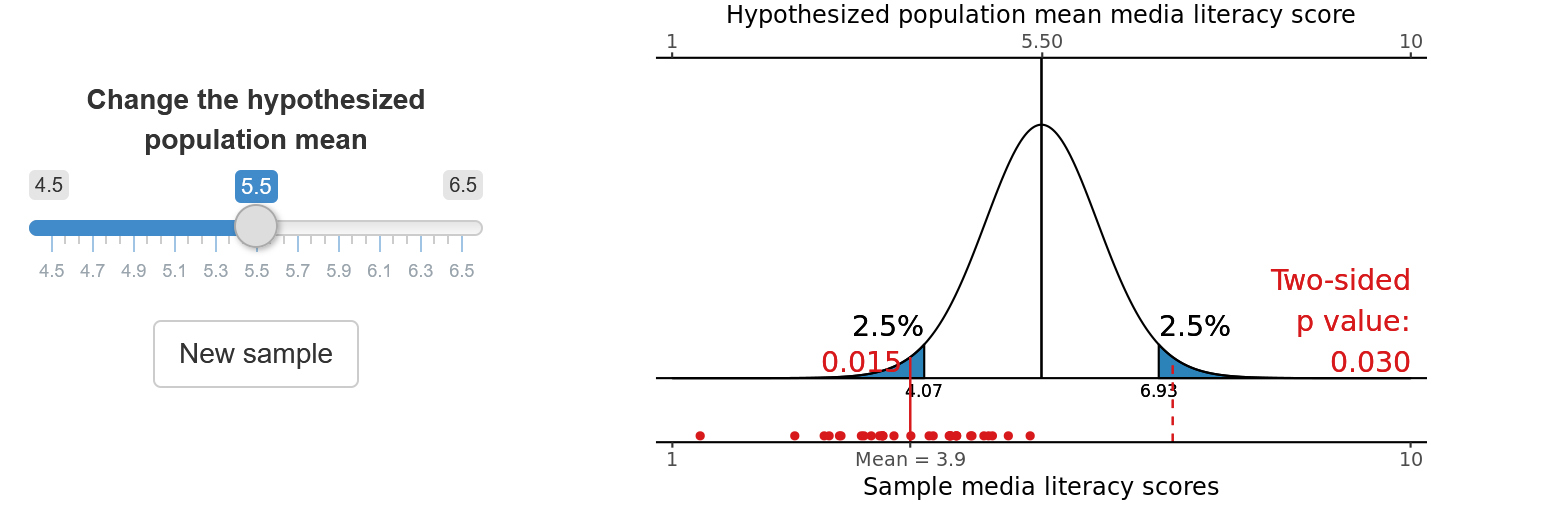
\includegraphics[width=420px]{GentleIntro_files/figure-latex/twosided-1} }\caption{Sampling distribution of average media literacy according to the null hypothesis.}\label{fig:twosided}
\end{figure}

\begin{enumerate}
\def\labelenumi{\arabic{enumi}.}
\tightlist
\item
  What does the number next to the solid red vertical line represent in
  Figure \ref{fig:twosided}?
\end{enumerate}

\begin{Shaded}
\begin{Highlighting}[]
\OperatorTok{*}\StringTok{ }\NormalTok{It represents the }\KeywordTok{probability}\NormalTok{ (p value) of drawing a sample with mean media}
\NormalTok{literacy below }\FloatTok{3.9} \ControlFlowTok{if}\NormalTok{ the null hypothesis is true that the population average}
\NormalTok{is }\FloatTok{5.50}\NormalTok{.}
\OperatorTok{*}\StringTok{ }\NormalTok{In a later section, we will see that this is a one}\OperatorTok{-}\NormalTok{sided p value, more}
\NormalTok{precisely, a left}\OperatorTok{-}\NormalTok{sided p value.}
\OperatorTok{*}\StringTok{ }\NormalTok{Please, do not forget to mention that this is the probability only }\ControlFlowTok{if}\NormalTok{ the}
\NormalTok{null hypothesis is true. See Question }\DecValTok{4}\NormalTok{.}
\end{Highlighting}
\end{Shaded}

\begin{enumerate}
\def\labelenumi{\arabic{enumi}.}
\setcounter{enumi}{1}
\tightlist
\item
  What is the relation between the number next to the solid red vertical
  line and the two-sided p value reported in the figure? Pay attention
  to the dashed red vertical line in your answer.
\end{enumerate}

\begin{Shaded}
\begin{Highlighting}[]
\OperatorTok{*}\StringTok{ }\NormalTok{The two}\OperatorTok{-}\NormalTok{sided p value is twice }\KeywordTok{the}\NormalTok{ (one}\OperatorTok{-}\NormalTok{sided) p value reported as number}
\ControlFlowTok{next}\NormalTok{ to the solid red line. Note that rounding errors occur.}
\OperatorTok{*}\StringTok{ }\NormalTok{The two}\OperatorTok{-}\NormalTok{sided p value tells us the probability of drawing a sample with}
\NormalTok{average media literacy at least as different from the hypothesized value as the}
\NormalTok{sample mean that we have found.}
\OperatorTok{*}\StringTok{ }\NormalTok{The solid red line represents the sample mean that we have found. The}
\NormalTok{associated probability tells us the probability of drawing a sample with}
\NormalTok{average media literacy at least }\FloatTok{5.5} \OperatorTok{-}\StringTok{ }\FloatTok{3.9}\NormalTok{ =}\StringTok{ }\FloatTok{1.6}\NormalTok{ LESS than the hypothesized}
\NormalTok{population value.}
\OperatorTok{*}\StringTok{ }\NormalTok{The dashed red line is the boundary }\ControlFlowTok{for}\NormalTok{ samples with average media literacy}
\NormalTok{that are at least }\FloatTok{1.6}\NormalTok{ HIGHER than the hypothesized population mean. These}
\NormalTok{samples are at least as far away from the hypothesis as the sample mean that we}
\NormalTok{have observed.}
\OperatorTok{*}\StringTok{ }\NormalTok{The dashed red line cuts off the same size from the right tail as the solid}
\NormalTok{red line cuts off from the left }\KeywordTok{tail}\NormalTok{ (}\ControlFlowTok{in}\NormalTok{ the initial situation of the figure).}
\NormalTok{In other words, it represents the same probability.}
\OperatorTok{*}\StringTok{ }\NormalTok{The two}\OperatorTok{-}\NormalTok{sided p value sums the probabilities cut off from the left tail and}
\NormalTok{the right tail. As a result, it is twice the probability reported }\ControlFlowTok{for}\NormalTok{ the left}
\NormalTok{tail.}
\end{Highlighting}
\end{Shaded}

\begin{enumerate}
\def\labelenumi{\arabic{enumi}.}
\setcounter{enumi}{2}
\tightlist
\item
  Is the test on average media literacy statistically significant in the
  initial situation of Figure \ref{fig:twosided}? If so, at which
  significance level? Use the rejection region, the number to the
  vertical red line, and the two-sided p value to motivate your answer.
\end{enumerate}

\begin{Shaded}
\begin{Highlighting}[]
\OperatorTok{*}\StringTok{ }\NormalTok{The statistical test is significant at the five per cent significance level.}
\OperatorTok{*}\StringTok{ }\NormalTok{Rejection region}\OperatorTok{:}\StringTok{ }\NormalTok{The sample mean is }\ControlFlowTok{in}\NormalTok{ the rejection region marked by the}
\NormalTok{blue tails, so the test is statistically significant. The total probability of}
\NormalTok{the two blue tails is five per cent, so this is the significance level.}
\OperatorTok{*}\StringTok{ }\NormalTok{(left}\OperatorTok{-}\NormalTok{sided) p Value}\OperatorTok{:}\StringTok{ }\NormalTok{The probability to draw a sample with }\FloatTok{3.9}\NormalTok{ average media}
\KeywordTok{literacy}\NormalTok{ (.}\DecValTok{015}\NormalTok{) is less than the probability associated with the rejection}
\NormalTok{region }\ControlFlowTok{in}\NormalTok{ the left }\KeywordTok{tail}\NormalTok{ (.}\DecValTok{025}\NormalTok{) }\ControlFlowTok{if}\NormalTok{ the null hypothesis is true. So the test is}
\NormalTok{statistically significant at the }\DecValTok{2} \OperatorTok{*}\StringTok{ }\NormalTok{.}\DecValTok{025}\NormalTok{ =}\StringTok{ }\NormalTok{.}\DecValTok{05}\NormalTok{ level.}
\OperatorTok{*}\StringTok{ }\NormalTok{Two}\OperatorTok{-}\NormalTok{sided p value}\OperatorTok{:}\StringTok{ }\NormalTok{The two}\OperatorTok{-}\NormalTok{sided p value is below five percent }\ControlFlowTok{if}\NormalTok{ the null}
\NormalTok{hypothesis is true, so the test is statistically significant at the five}
\NormalTok{percent significance level.}
\end{Highlighting}
\end{Shaded}

\begin{enumerate}
\def\labelenumi{\arabic{enumi}.}
\setcounter{enumi}{3}
\tightlist
\item
  What happens to the two-sided p value if you change the hypothesized
  population mean?
\end{enumerate}

\begin{Shaded}
\begin{Highlighting}[]
\OperatorTok{*}\StringTok{ }\NormalTok{The two}\OperatorTok{-}\NormalTok{sided p value changes }\ControlFlowTok{if}\NormalTok{ we change the hypothesized population mean}
\NormalTok{with the slider. It becomes smaller }\ControlFlowTok{if}\NormalTok{ we move the hypothesized population}
\NormalTok{value away from the observed sample mean. It becomes larger }\ControlFlowTok{if}\NormalTok{ we move towards}
\NormalTok{the sample mean.}
\OperatorTok{*}\StringTok{ }\NormalTok{This clearly illustrates that the p value of a test, the location of the}
\NormalTok{rejection regions, and, as a consequence, the statistical significance of the}
\NormalTok{test depends on the value of the population statistic that we specify }\ControlFlowTok{in}\NormalTok{ the}
\NormalTok{null hypothesis.}
\end{Highlighting}
\end{Shaded}

In the previous section, we learned that a test is statistically
significant if the sample statistic is in the rejection region.
Statistical software, however, usually does not report the rejection
region for the sample statistic. Instead, it reports the \emph{p value}
of the test, which is sometimes referred to as \emph{significance} or
\emph{Sig.} in SPSS.

A p value is the probability that a sample is drawn with a value for the
sample statistic that is at least as different from the hypothesized
population value as the value in the observed sample. In other words,
the p value tells us which proportion of all possible samples are less
similar to the hypothesized population value than our observed sample if
the null hypothesis is true. If this proportion is very small, say less
than five percent, the sample that we have drawn is among the unlikely
samples.

And what do we do if our sample is among the unlikely ones? We reject
the null hypothesis because the test is statistically significant. The
decision rule is quite simple if we know the p value of a test: If the p
value is below the significance level (usually .05), we reject the null
hypothesis. Otherwise, we do not reject it.

\begin{quote}
If p is low, the null must go and the test is statistically significant.
\end{quote}

This is the golden rule of null hypothesis testing (although some argue
that the gold of this rule is fool's gold, see Chapter
\ref{crit-discus}).

It is important to remember that a p value is a probability \emph{under
the assumption that the null hypothesis is true}. Therefore, it is a
\emph{conditional probability}.

Compare it to the probability that we throw sixes with a dice. This
probability is one out of six under the assumption that the dice is
unbiased. Probabilities always rest on assumptions. If the assumptions
are violated, we cannot calculate probabilities.

If the dice is biased, we don't know the probability of throwing sixes.
In the same way, we have no clue whatsoever of the probability of
drawing a sample like the one we have if the null hypothesis is not true
in the population. This is why specifying a null hypothesis is necessary
for calculating p values.

\section{Research hypothesis, alternative hypothesis, and nil
hypothesis}\label{null-alt}

The null hypothesis is central to significance testing. If the test is
statistically significant, that is, if the p value is below the
significance level, we reject the null hypothesis.

Statistical hypotheses, however, come in pairs: a null hypothesis
(\emph{H}\textsubscript{0}) and an \emph{alternative hypothesis}
(\emph{H}\textsubscript{1} or \emph{H}\textsubscript{A}). \emph{The
alternative hypothesis covers all situations not covered by the null
hypothesis}. The null hypothesis stating that average media literacy in
a population of children is 5.5, is paired with the alternative
hypothesis stating that the average is not 5.5. In this way, we cover
all possible outcomes.

If we reject the null hypothesis, we say that we accept the alternative
hypothesis. We believe that the alternative hypothesis is true, because
we do not believe that the null hypothesis is true. Of course, we know
that our belief can be mistaken. There is five per cent chance that we
rejected a null hypothesis that is actually true (Type I error, Section
\ref{sig-typeI}). Accepting the alternative hypothesis does not mean
that this hypothesis is true. Please, never forget this.

\begin{enumerate}
\def\labelenumi{\arabic{enumi}.}
\item
  Have another look at the research hypotheses. Which ones are null
  hypotheses, which ones are alternative hypotheses? Remember: A null
  hypothesis must specify a value for the population statistic that we
  are interested in.

  \begin{itemize}
  \item
    a television station reaches half of all households in a country,
  \item
    media literacy is below 5.5 (on a 10-point scale) among children,
  \item
    opinions about immigrants are not equally polarized among young and
    old voters,
  \item
    the celebrity endorsing a fundraising campaign makes a difference to
    adult's willingness to donate,
  \item
    more exposure to brand advertisements increases brand awareness of
    consumers.
  \end{itemize}
\end{enumerate}

\begin{Shaded}
\begin{Highlighting}[]
\OperatorTok{*}\StringTok{ }\NormalTok{A television station reaches half of all households }\ControlFlowTok{in}\NormalTok{ a country}\OperatorTok{:}\StringTok{ }\NormalTok{This}
\NormalTok{hypothesis is about a }\KeywordTok{proportion}\NormalTok{ (share) }\ControlFlowTok{in}\NormalTok{ the population of all households }\ControlFlowTok{in}
\NormalTok{a country. It specifies one particular value, namely }\StringTok{'half'}\NormalTok{, that is }\DecValTok{50}\NormalTok{% or}
\FloatTok{0.50}\NormalTok{. This reseach hypothesis is a null hypothesis.}
\OperatorTok{*}\StringTok{ }\NormalTok{Media literacy is below }\FloatTok{5.5}\NormalTok{ (on a }\DecValTok{10}\OperatorTok{-}\NormalTok{point scale) among children}\OperatorTok{:}\StringTok{ }\NormalTok{This}
\NormalTok{hypothesis addresses a population mean. It expects some value below }\FloatTok{5.5}\NormalTok{. This}
\NormalTok{can be more than one value, so this is an alternative hypothesis.}
\OperatorTok{*}\StringTok{ }\NormalTok{Opinions about immigrants are not equally polarized among young and old}
\NormalTok{voters}\OperatorTok{:}\StringTok{ }\NormalTok{This hypothesis is about variation }\ControlFlowTok{in}\NormalTok{ scores, }\ControlFlowTok{for}\NormalTok{ example the variance}
\ControlFlowTok{in}\NormalTok{ opinion scores. There is a variance }\ControlFlowTok{for}\NormalTok{ young voters and a variance }\ControlFlowTok{for}\NormalTok{ old}
\NormalTok{voters }\ControlFlowTok{in}\NormalTok{ the population and they are expected not to be equal. The difference}
\ControlFlowTok{in}\NormalTok{ variances, which is the statistic that we are interested }\ControlFlowTok{in}\NormalTok{ here, is not}
\NormalTok{expected to be zero. It is expected to be anything but zero. This can be more}
\NormalTok{than one value, so this is an alternative hypothesis.}
\OperatorTok{*}\StringTok{ }\NormalTok{The celebrity endorsing a fundraising campaign makes a difference to}
\NormalTok{willingness to donate}\OperatorTok{:}\StringTok{ }\NormalTok{We are probably going to compare the mean willingness}
\NormalTok{across groups of people. The means are not expected to be the same, but the}
\NormalTok{exact difference is not specified. It can be any number other than zero.}
\NormalTok{Again, this is the alternative hypothesis.}
\OperatorTok{*}\StringTok{ }\NormalTok{More exposure to brand advertisements increases brand awareness}\OperatorTok{:}\StringTok{ }\NormalTok{We expect a}
\NormalTok{positive association, but the researcher does not specify a value }\ControlFlowTok{for}\NormalTok{ the}
\NormalTok{expected association, so this is an alternative hypothesis.}
\end{Highlighting}
\end{Shaded}

The alternative hypothesis is mainly of interest because it usually
represents the research hypothesis (but not always as some statistics
textbooks would have us believe). Most of the research hypotheses in
social research are alternative hypotheses because our theories tell us
to expect differences or changes but not the size of differences or
changes.

Not knowing which precise difference or association to expect, we
usually formulate the research hypothesis that there is a difference or
association. Because a particular value for the difference or
association cannot be specified, these research hypotheses are
alternative hypotheses. The associated null hypothesis is that there is
no difference or no association. It equates the population statistic to
one value, namely zero. This type of null hypothesis is called a
\emph{nil hypothesis} or just plainly \emph{the nil}.

When groups have the same average scores on a dependent variable, for
example, willingness to donate to a charity, the differences between the
group averages are hypothesized to be zero. If there is no correlation
between exposure and brand awareness in the population, the correlation
coefficient (Spearman's rho or Pearson's correlation coefficient) or
regression coefficient (\(b\) or \(b^*\)) is hypothesized to be zero.
For all measures of association, zero means that there is no
association.

If the research hypothesis is the alternative hypothesis, we have to
formulate the null hypothesis ourselves. This is very important, because
the null hypothesis is actually tested. If statistical software does not
report the null hypothesis that is being tested, you may assume that it
equates the parameter of interest to zero (see Section \ref{nullSPSS} on
null hypotheses in SPSS).

\section{One-Sided and Two-Sided Tests}\label{one-twosidedtests}

In the preceding section, you may have felt a bit awkward when you were
determining whether a research hypothesis is a null hypothesis or an
alternative hypothesis. The research hypothesis stating that average
media literacy is below 5.5 in the population, for example, represents
the alternative hypothesis because it does not fix the hypothesized
population value to one number. The accompanying null hypothesis must
cover all other options, so it must state that the population mean is
5.5 or higher. But this null hypothesis does not specify one value as it
should, right?

This null hypothesis is slightly different from the ones we have
encountered so far, which equated the population value to a single
value. If the null hypothesis equates a parameter to a single value, the
null hypothesis can be rejected if the sample statistic is either too
high or too low. There are two ways of rejecting the null hypothesis, so
this type of hypothesis and test are called \emph{two-sided} or
\emph{two-tailed}.

By contrast, the null hypothesis stating that the population mean is 5.5
or higher is a \emph{one-sided} or \emph{one-tailed} hypothesis. It can
only be rejected if the sample statistic is at one side of the spectrum:
only below (left-sided) or only above (right-sided) the hypothesized
population value. In the media literacy example, the null hypothesis is
only rejected if the sample mean is well below the hypothesized
population value. A test of a one-sided null hypothesis is called a
\emph{one-sided test}.

\begin{figure}[H]
\href{http://82.196.4.233:3838/apps/nonsig-1sided/}{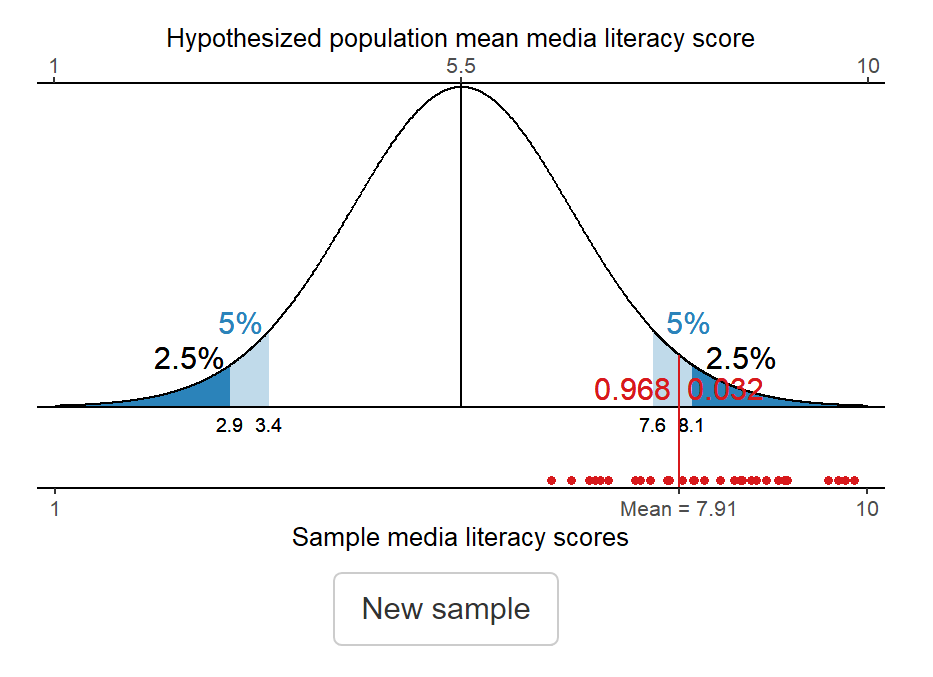
\includegraphics[width=420px]{GentleIntro_files/figure-latex/nonsig-1sided-1} }\caption{One-sided and two-sided tests of a null hypothesis.}\label{fig:nonsig-1sided}
\end{figure}

\begin{enumerate}
\def\labelenumi{\arabic{enumi}.}
\tightlist
\item
  The sampling distribution in Figure \ref{fig:nonsig-1sided} contains
  dark-blue tails that represent 2.5 per cent of the sampling
  distribution and light-blue tails representing five per cent of the
  sampling distribution. Note that the light-blue (5\%) tails include
  the dark-blue (2.5\%) tails. Which coloured tails do we use for a
  two-sided test, a left-sided test, and a right-sided test at a five
  per cent significance level?
\end{enumerate}

\begin{Shaded}
\begin{Highlighting}[]
\OperatorTok{*}\StringTok{ }\NormalTok{As we learned }\ControlFlowTok{in}\NormalTok{ a previous section, a two}\OperatorTok{-}\NormalTok{sided test divides the total}
\NormalTok{significance level into two parts, one half }\ControlFlowTok{for}\NormalTok{ each tail of the sampling}
\NormalTok{distribution. The dark blue tails, each representing }\FloatTok{2.5}\NormalTok{ per cent, then, are}
\NormalTok{used }\ControlFlowTok{for}\NormalTok{ a two}\OperatorTok{-}\NormalTok{tailed test at five per cent significance level.}
\OperatorTok{*}\StringTok{ }\NormalTok{A one}\OperatorTok{-}\NormalTok{tailed test takes into account sample outcomes either below the}
\NormalTok{hypothesized value or above the hypothesized value. It assigns the full}
\NormalTok{significance }\KeywordTok{level}\NormalTok{ (}\DecValTok{5}\NormalTok{%) to one tail, so it uses the light blue }\KeywordTok{tails}\NormalTok{ (which}
\NormalTok{include the dark blue tails).}
\OperatorTok{*}\StringTok{ }\NormalTok{A left}\OperatorTok{-}\NormalTok{sided test only uses the light blue tail at the left, a right}\OperatorTok{-}\NormalTok{sided}
\NormalTok{test only uses the tail at the right.}
\end{Highlighting}
\end{Shaded}

\begin{enumerate}
\def\labelenumi{\arabic{enumi}.}
\setcounter{enumi}{1}
\tightlist
\item
  Practice recognizing significant test results in Figure
  \ref{fig:nonsig-1sided}. Draw some samples and decide if a two-sided,
  right-sided, or left-sided test is statistically significant at the
  5\% significance level.
\end{enumerate}

\begin{Shaded}
\begin{Highlighting}[]
\OperatorTok{*}\StringTok{ }\NormalTok{If the sample mean falls within a dark}\OperatorTok{-}\NormalTok{blue tail, a two}\OperatorTok{-}\NormalTok{sided test is}
\NormalTok{statistically significant.}
\OperatorTok{*}\StringTok{ }\NormalTok{If the sample mean is falls within the }\KeywordTok{light}\NormalTok{ (or dark}\OperatorTok{-}\NormalTok{blue) tail at the}
\NormalTok{right, a right}\OperatorTok{-}\NormalTok{sided test is statistically significant but a left}\OperatorTok{-}\NormalTok{sided test}
\NormalTok{is not.}
\OperatorTok{*}\StringTok{ }\NormalTok{If the sample mean is falls within the }\KeywordTok{light}\NormalTok{ (or dark}\OperatorTok{-}\NormalTok{blue) tail at the}
\NormalTok{left, a left}\OperatorTok{-}\NormalTok{sided test is statistically significant but a right}\OperatorTok{-}\NormalTok{sided test is}
\NormalTok{not.}
\end{Highlighting}
\end{Shaded}

\begin{enumerate}
\def\labelenumi{\arabic{enumi}.}
\setcounter{enumi}{2}
\tightlist
\item
  In which situation is a one-sided test statistically significant
  whereas a two-sided test is not statistically significant at the five
  per cent significance level?
\end{enumerate}

\begin{Shaded}
\begin{Highlighting}[]
\OperatorTok{*}\StringTok{ }\NormalTok{If the sample mean is }\ControlFlowTok{in}\NormalTok{ the light}\OperatorTok{-}\NormalTok{blue part of the tail at the right but not}
\ControlFlowTok{in}\NormalTok{ the dark}\OperatorTok{-}\NormalTok{blue part, a right}\OperatorTok{-}\NormalTok{sided test is statistically significant but a}
\NormalTok{two}\OperatorTok{-}\NormalTok{sided test is not.}
\OperatorTok{*}\StringTok{ }\NormalTok{If the sample mean is }\ControlFlowTok{in}\NormalTok{ the light}\OperatorTok{-}\NormalTok{blue part of the tail at the left but not}
\ControlFlowTok{in}\NormalTok{ the dark}\OperatorTok{-}\NormalTok{blue part, a left}\OperatorTok{-}\NormalTok{sided test is statistically significant but a}
\NormalTok{two}\OperatorTok{-}\NormalTok{sided test is not.}
\end{Highlighting}
\end{Shaded}

\begin{enumerate}
\def\labelenumi{\arabic{enumi}.}
\setcounter{enumi}{3}
\tightlist
\item
  In which situation is a one-sided test not statistically significant
  whereas a two-sided test is statistically significant at the five per
  cent significance level?
\end{enumerate}

\begin{Shaded}
\begin{Highlighting}[]
\OperatorTok{*}\StringTok{ }\NormalTok{A one}\OperatorTok{-}\NormalTok{sided test is more easily statistically significant because the }\DecValTok{5}\NormalTok{%}
\NormalTok{part of the tail is wider than the }\FloatTok{2.5}\NormalTok{% part of the tail. But a one}\OperatorTok{-}\NormalTok{sided test}
\NormalTok{requires that the sample outcome is on the right side of the hypothesized}
\NormalTok{value. If it is on the wrong side, it can never be significant }\ControlFlowTok{in}\NormalTok{ a one}\OperatorTok{-}\NormalTok{tailed}
\NormalTok{test. If the researcher wants to reject the null hypothesis only }\ControlFlowTok{if}\NormalTok{ the sample}
\NormalTok{outcome is too high, she will not reject it }\ControlFlowTok{if}\NormalTok{ the sample outcome is too low.}
\OperatorTok{*}\StringTok{ }\NormalTok{If the sample mean is }\ControlFlowTok{in}\NormalTok{ the dark}\OperatorTok{-}\NormalTok{blue tail at the right, a two}\OperatorTok{-}\NormalTok{sided test}
\NormalTok{is statistically significant but a left}\OperatorTok{-}\NormalTok{sided test is not. The right tail is}
\NormalTok{the wrong side }\ControlFlowTok{for}\NormalTok{ a left}\OperatorTok{-}\NormalTok{sided hypothesis.}
\OperatorTok{*}\StringTok{ }\NormalTok{If the sample mean is }\ControlFlowTok{in}\NormalTok{ the dark}\OperatorTok{-}\NormalTok{blue tail at the left, a two}\OperatorTok{-}\NormalTok{sided test is}
\NormalTok{statistically significant but a right}\OperatorTok{-}\NormalTok{sided test is not. The left tail is the}
\NormalTok{wrong side }\ControlFlowTok{for}\NormalTok{ a right}\OperatorTok{-}\NormalTok{sided hypothesis.}
\end{Highlighting}
\end{Shaded}

In a left-sided test of the media literacy hypothesis, the researcher is
not interested in demonstrating that average media literacy among
children can be larger than 5.5. She only wants to test if it is below
5.5, perhaps because an average score below 5.5 is alarming and requires
an intervention, or because prior knowledge about the world has
convinced her that average media literacy among children can only be
lower than 5.5 on average in the population.

If it is deemed important to note values well over 5.5 as well as values
well below 5.5, the research and null hypotheses should be two-sided.
Then, a sample average well above 5.5 would also have resulted in a
rejection of the null hypothesis. In a left-sided test, however, a high
sample outcome cannot reject the null hypothesis.

\subsection{Boundary value as hypothesized population
value}\label{boundary-value-as-hypothesized-population-value}

\begin{figure}[H]
\href{http://82.196.4.233:3838/apps/sign-left/}{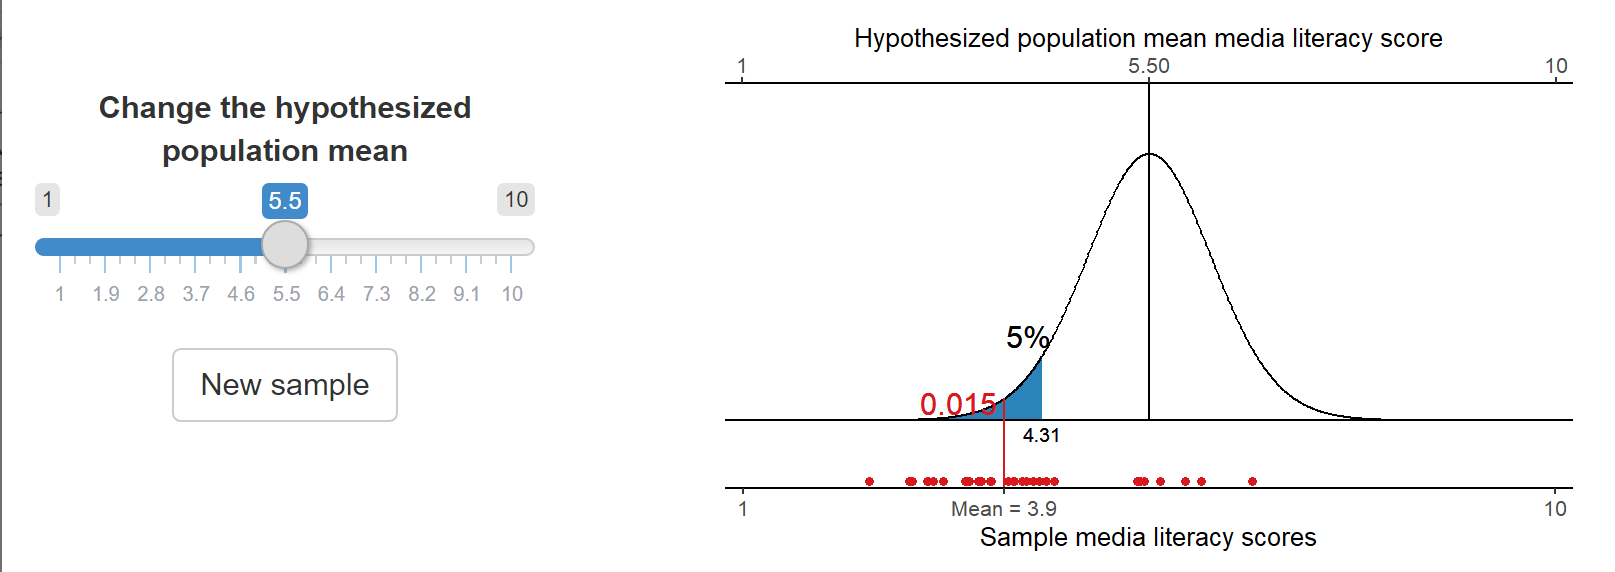
\includegraphics[width=420px]{GentleIntro_files/figure-latex/sign-left-1} }\caption{Sampling distribution of average media literacy.}\label{fig:sign-left}
\end{figure}

\begin{enumerate}
\def\labelenumi{\arabic{enumi}.}
\tightlist
\item
  Figure \ref{fig:sign-left} shows the sampling distribution and the
  rejection region for a left-sided test at five per cent significance
  level. If we reject the null hypothesis that average media literacy in
  the population is 5.5, do we also reject a null hypothesis that this
  average is larger than 5.5? Change the slider to demonstrate your
  answer.
\end{enumerate}

\begin{Shaded}
\begin{Highlighting}[]
\OperatorTok{*}\StringTok{ }\NormalTok{Yes. If a left}\OperatorTok{-}\NormalTok{sided test is situated }\ControlFlowTok{in}\NormalTok{ the rejection region with the null}
\NormalTok{hypothesis that the population mean is }\FloatTok{5.5}\NormalTok{, a left}\OperatorTok{-}\NormalTok{sided test is also situated}
\ControlFlowTok{in}\NormalTok{ the rejection region }\ControlFlowTok{for}\NormalTok{ higher values of the hypothesized population mean.}
\OperatorTok{*}\StringTok{ }\NormalTok{The sampling distribution shifts to the right }\ControlFlowTok{if}\NormalTok{ we use a higher value }\ControlFlowTok{for}
\NormalTok{the hypothesized population mean. The observed sample mean remains }\ControlFlowTok{in}\NormalTok{ the left}
\NormalTok{blue tail, which extends infinitely to the left, even }\ControlFlowTok{if}\NormalTok{ we cannot see that}
\NormalTok{clearly }\ControlFlowTok{in}\NormalTok{ the figure.}
\end{Highlighting}
\end{Shaded}

You may wonder how a one-sided null hypothesis equates the parameter of
interest with one value as it should. The special value here is 5.5. If
we can reject the null hypothesis stating that the population mean is
5.5 because our sample mean is sufficiently lower than 5.5, we can also
reject any hypothesis involving population means higher than 5.5.

In other words, if you want to know if the value is not 5.5 or more, it
is enough to find that it is less than 5.5. If it's less than 5.5, then
you know it's also less than any number above 5.5. Therefore, we use the
boundary value of a one-sided null hypothesis as the value for a
one-sided test.

\subsection{One-sided -- two-sided distinction is not always
relevant}\label{one-sided-two-sided-distinction-is-not-always-relevant}

Note that the difference between one-sided and two-sided tests is only
useful if we test a statistic against one particular value or if we test
the difference between two groups.

In the first situation, for example, if we test the null hypothesis that
average media literacy is 5.5 in the population, we may only be
interested in showing that the population value is lower than the
hypothesized value. Another example is a test on a regression
coefficient or correlation coefficient. According to the null
hypothesis, the coefficient is zero in the population. If we only want
to use a brand advertisement if exposure to the advertisement increases
brand awareness among consumers, we apply a right-sided test to the
coefficient for the effect of exposure on brand awareness because we are
only interested in a positive effect (larger than the zero).

In the second situation, we compare the scores of two groups on a
dependent variable. If we compare average media literacy after an
intervention to media literacy before the intervention (paired-samples t
test), we must demonstrate an increase in media literacy before we are
going to use the intervention on a large scale. Again, a one-sided test
can be applied.

In contrast, we cannot meaningfully formulate a one-sided null
hypothesis if we are comparing three groups or more. Even if we expect
that Group A can only score higher than Group B and Group C, what about
the difference between Group B and Group C? If we can't have meaningful
one-sided null hypotheses, we cannot meaningfully distinguish between
one-sided and two-sided null hypotheses.

\subsection{From one-sided to two-sided p values and back
again}\label{from-one-sided-to-two-sided-p-values-and-back-again}

Statistical software like SPSS usually reports either one-sided or
two-sided p values. What if a one-sided p value is reported but you need
a two-sided p value or the other way around?

In Figure \ref{fig:1-2sidedpvalues}, the sample mean is 5.15 and we have
.042 probability to find a sample mean of 5.15 or less if the null
hypothesis is true. This probability is the surface under the curve to
the left of the red line representing the sample mean. It is the
one-sided p value that we obtain if we only take into account the
possibility that the population mean can be smaller than the
hypothesized value. We are only interested in the left tail of the
sampling distribution.

\begin{figure}
\centering
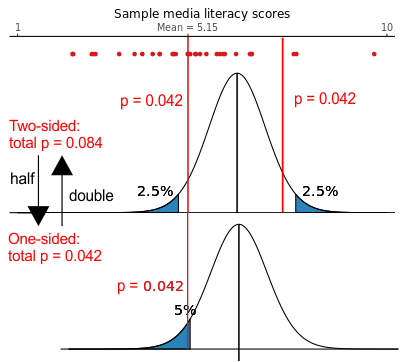
\includegraphics[width=300px]{figures/CH4.1_2sidedpvalues.png}
\caption{\label{fig:1-2sidedpvalues}Halve a two-sided p value to obtain a
one-sided p value, double a one-sided p value to obtain a two-sided p
value.}
\end{figure}

In a two-sided test, we have to reckon with two different types of
outcomes. Our sample oucome can be smaller or larger than the
hypothesized population value. As a consequence, the p value must cover
samples at opposite sides of the sampling distribution. We should not
only reckon with sample means that are less than 5.15 but also with
sample means that are just as much larger than the hypothesized
population value. So we have to take into account a probability of .042
for the right tail of the distribution as well in Figure
\ref{fig:1-2sidedpvalues}. We can double the one-sided p value to obtain
the two-sided p value.

In contrast, if our statistical software tells us the two-sided p value
and we want to have the one-sided p value, we can simply halve the
two-sided p value. The two-sided p value is divided equally between the
left and right tails. If we are interested in just one tail, we can
ignore the half of the p value that is situated in the other tail. Of
course, this only makes sense if a one-sided test makes sense.

Be careful if you divide a two-sided p value to obtain a one-sided p
value. If your left-sided test hypothesizes that average media literacy
is below 5.5 but your sample mean is well above 5.5, the two-sided p
value can be below .05. But your left-sided test can never be
significant because a sample mean above 5.5 is fully in line with the
null hypothesis. Check that the sample outcome is at the correct side of
the hypothesized population value.

\section{Testing a Null Hypothesis with a Theoretical Probability
Distribution}\label{testing-a-null-hypothesis-with-a-theoretical-probability-distribution}

The preceding sections taught us how to execute a significance test.
Formulate a null hypothesis that equates a population characteristic
(parameter) to a particular value, which is a boundary value in the case
of a one-sided test. Then construct a sampling distribution with the
hypothesized (boundary) value as centre and use it to calculate a p
value. If the p value is below the significance level (\(\alpha\)), the
test is statistically significant, so we reject the null hypothesis.

We have not discussed yet how we construct the sampling distribution.
Chapter \ref{probmodels} presented three ways: bootstrapping, an exact
approach, and approximation of the sampling distribution with a
theoretical probability distribution. The last option is the most
popular, so let us discuss it first. Exact approaches and bootstrapping
are discussed in the next section.

A theoretical probability distribution links sample outcomes such as a
sample mean to probabilities by means of a \emph{test statistic}. A test
statistic is named after the theoretical probability distribution to
which it belongs: \emph{z} for the standard-normal or \emph{z}
distribution, \emph{t} for the \emph{t} distribution, \emph{F} for the
\emph{F} distribution and, you guessed it, chi-squared for the
chi-squared distribution.

\begin{figure}[H]
\href{http://82.196.4.233:3838/apps/crit-df/}{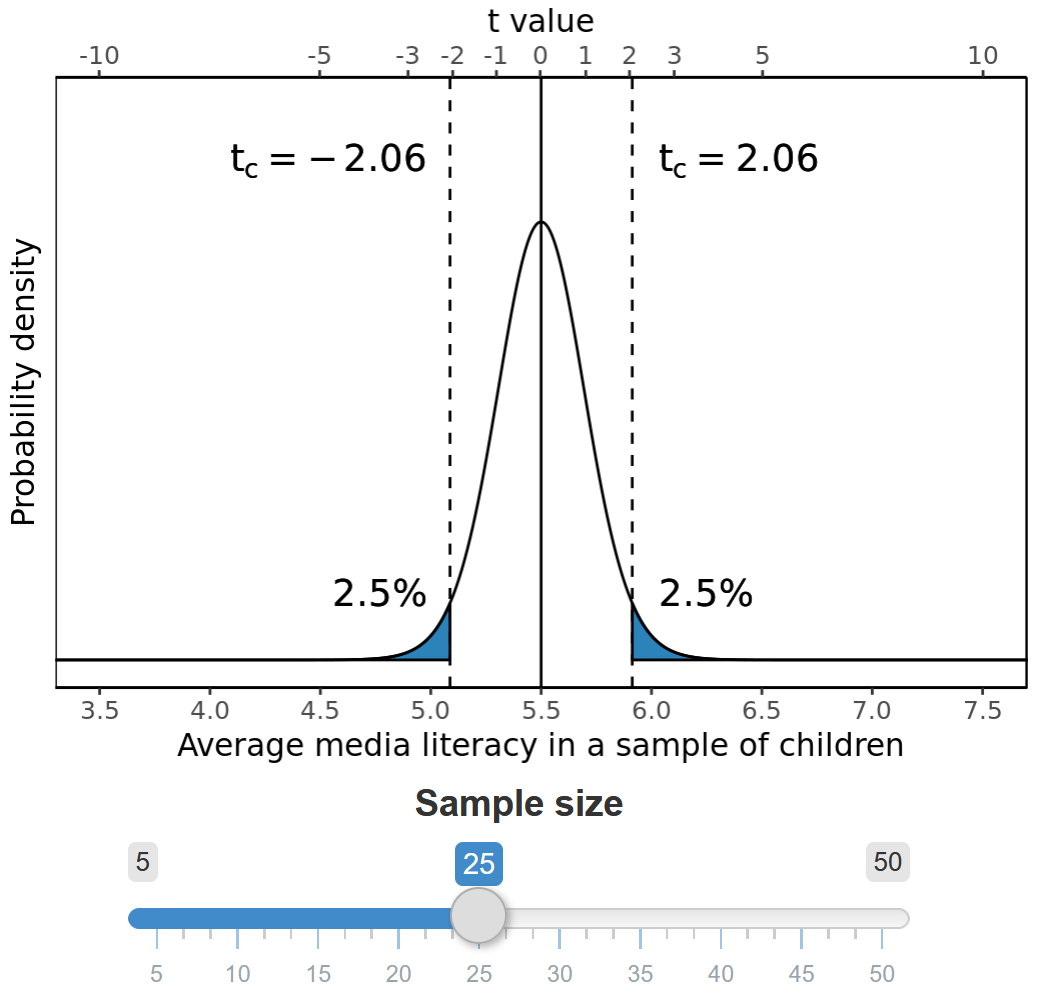
\includegraphics[width=420px]{GentleIntro_files/figure-latex/crit-df-1} }\caption{Sample size and critical values in a one-sample t test on the null hypothesis that the population average is 5.5.}\label{fig:crit-df}
\end{figure}

Figure \ref{fig:crit-df} uses the t distribution to approximate the
sampling distribution of average media literacy in a random sample of
children. The null hypothesis states that average media literacy is 5.5
in the population of children.

\begin{enumerate}
\def\labelenumi{\arabic{enumi}.}
\tightlist
\item
  What is the meaning of the coloured tails?
\end{enumerate}

\begin{Shaded}
\begin{Highlighting}[]
\OperatorTok{*}\StringTok{ }\NormalTok{The coloured tails represent the probabilities of drawing a sample with a}
\NormalTok{(sample) mean that differs a lot from }\KeywordTok{the}\NormalTok{ (true or hypothesized) population}
\NormalTok{mean. }\KeywordTok{The}\NormalTok{ (true or hypothesized) population mean is represented by the centre}
\NormalTok{of the distribution.}
\OperatorTok{*}\StringTok{ }\NormalTok{In this case, the probabilities of the two coloured tails sum to }\DecValTok{5}\NormalTok{%, so the}
\NormalTok{tails represent the top five per cent of samples that are most different from}
\NormalTok{the hypothesized or true population mean.}
\end{Highlighting}
\end{Shaded}

\begin{enumerate}
\def\labelenumi{\arabic{enumi}.}
\setcounter{enumi}{1}
\tightlist
\item
  What is the meaning of t\textsubscript{c}?
\end{enumerate}

\begin{Shaded}
\begin{Highlighting}[]
\OperatorTok{*}\StringTok{ }\NormalTok{t}\OperatorTok{~}\NormalTok{c}\OperatorTok{~}\StringTok{ }\NormalTok{is the value of the test statistic t that separates the most unlikely}
\NormalTok{or most extreme samples from the most likely samples.}
\OperatorTok{*}\StringTok{ }\NormalTok{It is called the critical value of the test statistic.}
\end{Highlighting}
\end{Shaded}

\begin{enumerate}
\def\labelenumi{\arabic{enumi}.}
\setcounter{enumi}{2}
\tightlist
\item
  Why does the distribution become more pointed when sample size
  increases?
\end{enumerate}

\begin{Shaded}
\begin{Highlighting}[]
\OperatorTok{*}\StringTok{ }\NormalTok{With a larger sample, we have more information, so we have more precise}
\NormalTok{results. More sample means are close to the true population mean.}
\OperatorTok{*}\StringTok{ }\NormalTok{In technical terms, the variation of sample means decreases with larger}
\NormalTok{sample size; sample means are more alike. The standard deviation of the}
\NormalTok{sampling distribution measures the variation of sample means. It is the}
\NormalTok{standard error of the sampling }\KeywordTok{distribution}\NormalTok{ (see the preceding chapter). A}
\NormalTok{distribution of larger samples has a smaller standard error.}
\end{Highlighting}
\end{Shaded}

\begin{enumerate}
\def\labelenumi{\arabic{enumi}.}
\setcounter{enumi}{3}
\tightlist
\item
  Is there a fixed relation between the t values (top axis) and the
  values for average sample media literacy (bottom axis)? Change the
  sample size to find the answer.
\end{enumerate}

\begin{Shaded}
\begin{Highlighting}[]
\OperatorTok{*}\StringTok{ }\NormalTok{No, there is not a fixed relation. A particular average media literacy}
\NormalTok{score, }\ControlFlowTok{for}\NormalTok{ example, }\FloatTok{4.0}\NormalTok{ on the bottom scale, does not always correspond to the}
\NormalTok{same test }\KeywordTok{statistic}\NormalTok{ (t) value on the top scale. Just change sample size to see}
\NormalTok{this.}
\end{Highlighting}
\end{Shaded}

\begin{enumerate}
\def\labelenumi{\arabic{enumi}.}
\setcounter{enumi}{4}
\tightlist
\item
  What is the relation between sample size and critical t values?
\end{enumerate}

\begin{Shaded}
\begin{Highlighting}[]
\OperatorTok{*}\StringTok{ }\NormalTok{Smaller samples have slightly larger critical t values.}
\end{Highlighting}
\end{Shaded}

A test statistic is calculated from the sample statistic that we want to
test, for instance, the sample proportion, mean, variance, or
association, but it uses the null hypothesis as well. A test statistic
more or less standardizes the difference between the sample statistic
and the population value that we expect under the null hypothesis.

The exact formula and calculation of a test statistic is not important
to us. Just note that the test statistic is zero if the sample outcome
is equal to the hypothesized population value. In Figure
\ref{fig:crit-df}, for example, the t value of a sample with mean 5.5 is
zero if the hypothesized population mean is 5.5. The larger the
difference between the observed value (sample outcome) and the expected
value (hypothesized population value), the more extreme the value of the
test statistic, the less likely (lower p value) it is that we draw a
sample with the observed outcome or an outcome even more different from
the expected value, and, finally, the more likely we are to reject the
null hypothesis.

We reject the null hypothesis if the test statistic is in the
\emph{rejection region}. The value of the test statistic where the
rejection region starts, is called the \emph{critical value} of the test
statistic. In Section \ref{crit-values}, we learned that 1.96 is the
critical value of z for a two-sided test at five per cent significance
level in a standard-normal distribution. In a z test, then, a sample z
value above 1.96 or below -1.96 indicates a statistically significant
test result.

Probability distributions other than the standard-normal distribution,
however, do not have fixed critical values. Their critical values depend
on the \emph{degrees of freedom} of the test, usually abbreviated to
\emph{df}. The degrees of freedom of a test may depend on sample size,
the number of groups that we compare, or the number of rows and columns
in a contingency table. We don't need to worry about this.

The t distribution is an example of a probability distribution for which
the critical values depend on the degrees of freedom of the test. In
this case, the degrees of freedom are determined by sample size. Larger
samples have more degrees of freedom and, as a consequence, they have
slightly lower critical values. For samples that are not too small the
critical values of t are near 2. You may have noticed this in Figure
\ref{fig:crit-df}.

APA6 requires us to report the degrees of freedom. If SPSS reports the
degrees of freedom, usually in a column with the header \emph{df}, you
should include the number between brackets after the name of the test
statistic. If, for example, a t test has 18 degrees of freedom and the t
value is 0.63, you report: \emph{t} (18) = 0.63. Note that the \emph{F}
test statistic has two degrees of freedom, both of which should be
reported (separated by a comma and a blank space), for example, \emph{F}
(2, 87) = 3.13.

\section{Testing a Null Hypothesis with an Exact Approach or
Bootstrapping}\label{testing-a-null-hypothesis-with-an-exact-approach-or-bootstrapping}

Exact approaches calculate probabilities for discrete outcomes. In the
candy example, the number of yellow candies in a sample bag of ten
candies is a discrete outcome. With the binomial formula, the exact
probability of zero yellow candies can be calculated, the probability of
one yellow candy, two yellow candies, and so on (see Figure
\ref{fig:exactapproachfigure}).

Let us image that our sample bag contains six yellow candies and we
hypothesize that twenty per cent of the candies are yellow in the
population. The p value of our sample outcome (six yellow candies) sums
the probabilities of drawing a sample bag with six, seven, eight, nine,
or ten yellow candies from a population in which twenty per cent of the
candies are yellow (our null hypothesis). The p value happens to be
.006, even though Figure \ref{fig:exactapproachfigure} suggests .007 but
that is a matter of rounding error. This is the right-sided p value if
we assume that our hypothesis is true.

With the p value, we execute the significance test as usual. The p value
is well below the significance level of .05, so we reject the null
hypothesis that twenty per cent of all candies in the population are
yellow.

The situation is slightly more complicated if we want to execute a
significance test with a sampling distribution created with
bootstrapping. To understand the testing procedure with bootstrapping,
we first have to discuss the relation between null-hypothesis testing
and confidence intervals.

\subsection{Relation between null-hypothesis tests and confidence
intervals}\label{null-ci0}

The top of Figure \ref{fig:null-ci} shows media literacy scores in a
random sample of children and their average media literacy score (red).
The hypothesized average media literacy in the population of children is
shown on the bottom axis. The curve represents the sampling distribution
if the null hypothesis is true.

\begin{figure}[H]
\href{http://82.196.4.233:3838/apps/null-ci/}{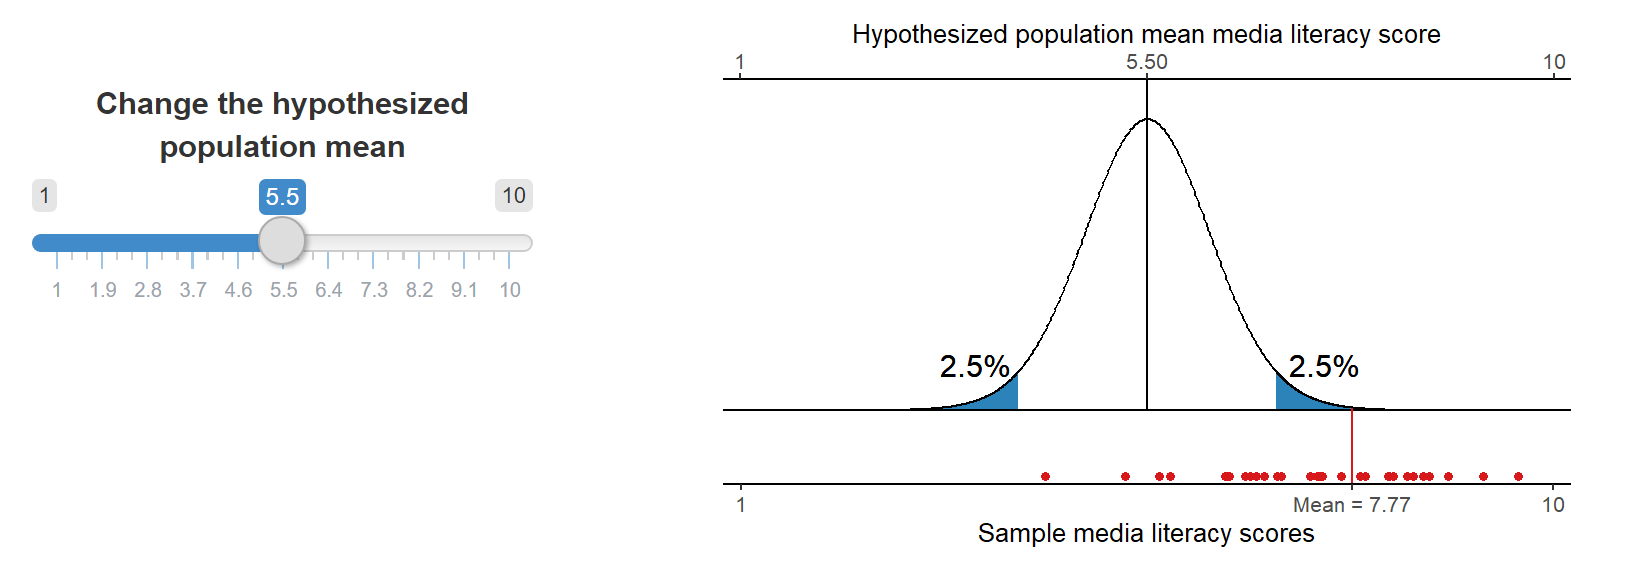
\includegraphics[width=420px]{GentleIntro_files/figure-latex/null-ci-1} }\caption{How does null hypothesis significance relate to confidence intervals?}\label{fig:null-ci}
\end{figure}

\begin{enumerate}
\def\labelenumi{\arabic{enumi}.}
\tightlist
\item
  What are the lowest and highest hypothesized population means for
  which the null hypothesis is \emph{not} rejected?
\end{enumerate}

\begin{Shaded}
\begin{Highlighting}[]
\OperatorTok{*}\StringTok{ }\NormalTok{Change the slider such that the boundary of the right tail coincides with}
\NormalTok{the red line of the sample mean. This hypothesized population value is the}
\NormalTok{lower bound of the }\DecValTok{95}\NormalTok{% confidence interval. It is the lowest hypothesized}
\NormalTok{population value }\ControlFlowTok{for}\NormalTok{ which the observed sample mean is not statistically}
\NormalTok{significant.}
\OperatorTok{*}\StringTok{ }\NormalTok{Make the boundary of the left tail meet the sample }\KeywordTok{mean}\NormalTok{ (red line)}\OperatorTok{:}\StringTok{ }\NormalTok{this}
\NormalTok{population value is the upper bound of the confidence interval. It is the}
\NormalTok{highest hypothesized population value }\ControlFlowTok{for}\NormalTok{ which the observed sample mean is}
\NormalTok{not statistically significant.}
\end{Highlighting}
\end{Shaded}

\begin{enumerate}
\def\labelenumi{\arabic{enumi}.}
\setcounter{enumi}{1}
\tightlist
\item
  The interval between the lowest and highest hypothesized population
  means of Question 1 is the 95\% confidence interval (see Section
  \ref{ci-parameter}). Is a null hypothesis statistically significant if
  the hypothesized population value is within the 95\% confidence
  interval or outside of this interval?
\end{enumerate}

\begin{Shaded}
\begin{Highlighting}[]
\OperatorTok{*}\StringTok{ }\NormalTok{A confidence interval contains }\KeywordTok{all}\NormalTok{ (hypothetical) values of the population}
\NormalTok{value}\OperatorTok{---}\NormalTok{here}\OperatorTok{:}\StringTok{ }\NormalTok{the population mean}\OperatorTok{---}\ControlFlowTok{for}\NormalTok{ which the observed sample is}
\NormalTok{plausible, }\ControlFlowTok{for}\NormalTok{ example, it is among the }\DecValTok{95}\NormalTok{% of samples with values closest}
\NormalTok{to the population value.}
\OperatorTok{*}\StringTok{ }\NormalTok{We reject a null hypothesis }\ControlFlowTok{if}\NormalTok{ the sample is NOT plausible when the null}
\NormalTok{hypothesis is true. So we reject null hypotheses }\ControlFlowTok{if}\NormalTok{ the hypothesized population}
\NormalTok{value is OUTSIDE the confidence interval. If it is INSIDE the confidence}
\NormalTok{interval, we do NOT reject the null hypothesis.}
\end{Highlighting}
\end{Shaded}

Do you remember how we constructed a confidence interval in Chapter
\ref{param-estim}? We looked for all population values for which the
sample outcome is sufficiently plausible. Sufficiently plausible means
that our observed sample outcome is among the sample outcomes that are
closest to the population value. By convention, we use a confidence
level of 95 per cent, which means that our observed sample is among the
95 per cent of all samples that have outcomes closest to the population
value.

But wait a minute. If the sample outcome is among the 95 per cent of
samples in the middle of the sampling distribution, it is not among the
extreme five percent of all samples. This is simply another way of
saying that the observed sample outcome is not statistically significant
at the five per cent level. A 95\% confidence interval contains all
population values that we could hypothesize for which our sample outcome
is not statistically significant.

\begin{quote}
A 95\% confidence interval contains all null hypotheses that would not
be rejected with the current sample at the 5\% significance level,
two-sided.
\end{quote}

If we know the 95\% confidence interval, we can immediately see if our
null hypothesis must be rejected or not. If the population value in our
null hypothesis lies within the 95\% confidence interval, the null
hypothesis is NOT rejected. The sample that we have drawn is
sufficiently plausible if our null hypothesis is true. In contrast, we
must reject the null hypothesis if the hypothesized population value is
NOT in the 95\% confidence interval.

Let us assume, for example, that average media literacy in our sample is
3.0 and that the 95\% confidence interval for average media literacy
ranges from 1.0 to 5.0. A null hypothesis specifying 2.5 as population
average must not be rejected at the five percent significance level
because 2.5 is in between 1.0 and 5.0, that is, inside the 95\%
confidence interval. If our null hypothesis says that average media
literacy in the population is 5.5, we must reject this null hypothesis
because it is outside the 95\% confidence interval. The null hypothesis
that average media literacy in the population is 0.0 must be rejected
for the same reason.

Note that the hypothesized value can be too high or too low for the
confidence interval, so a hypothesis test using a confidence interval is
always two-sided.

\subsection{Testing a null hypothesis with
bootstrapping}\label{testing-a-null-hypothesis-with-bootstrapping}

Using the confidence interval is the easiest and sometimes the only way
of testing a null hypothesis if we create the sampling distribution with
bootstrapping. For instance, we may use the median as the preferred
measure of central tendency rather than the mean if the distribution of
scores is quite skewed and the sample is not very large. In this
situation, a theoretical probability distribution for the sample median
is not known, so we resort to bootstrapping.

Bootstrapping creates an empirical sampling distribution: a lot of
samples with a median calculated for each sample. A confidence interval
can be created from this sampling distribution (see Section
\ref{bootstrap-confidenceinterval}). If our null hypothesis about the
population median is included in the 95\% confidence interval, we do not
reject the null hypothesis. Otherwise, we reject it.

\section{Test Recipe and Rules for
Reporting}\label{test-recipe-and-rules-for-reporting}

Testing a null hypothesis consists of several steps, which are
summarized below, much like a recipe in a cookbook.

\begin{enumerate}
\def\labelenumi{\arabic{enumi}.}
\tightlist
\item
  Specify the statistical hypotheses.
\end{enumerate}

In the first step, translate the research hypothesis into a null and
alternative hypothesis. This requires choosing the right statistic for
testing the research hypothesis (Section \ref{nullhypothesis}) and
choosing between a one-sided or two-sided test if applicable (Section
\ref{one-twosidedtests}).

\begin{enumerate}
\def\labelenumi{\arabic{enumi}.}
\setcounter{enumi}{1}
\tightlist
\item
  Select the significance level of the test.
\end{enumerate}

Before we execute the test, we have to choose the maximum probability of
rejecting the null hypothesis if it is actually true. This is the
significance level of the test. We almost always select .05 (5\%) as the
significance level. If we have a very large sample, e.g., several
thousands of cases, we may select a lower significance level, for
instance, 0.01. See Chapter \ref{power} for more details.

\begin{enumerate}
\def\labelenumi{\arabic{enumi}.}
\setcounter{enumi}{2}
\tightlist
\item
  Select how the sampling distribution is created.
\end{enumerate}

Are you going to use bootstrapping, an exact approach, or a theoretical
probability distribution? Theoretical probability distributions are the
most common choice. We have to know which theoretical probability
distribution can be used for which test. If you are working with
statistical software, you automatically select the correct probability
distribution by selecting the correct test. For example, a test on the
means of two independent samples in SPSS uses the t distribution.

\begin{enumerate}
\def\labelenumi{\arabic{enumi}.}
\setcounter{enumi}{3}
\tightlist
\item
  Execute the test.
\end{enumerate}

Let your statistical software calculate the p value of the test and/or
the value of the test statistic. It is important that this step comes
after the first three steps. The first three steps should be made
without knowledge of the results in the sample.

\begin{enumerate}
\def\labelenumi{\arabic{enumi}.}
\setcounter{enumi}{4}
\tightlist
\item
  Decide on the null hypothesis.
\end{enumerate}

Reject the null hypothesis if the p value is lower than the significance
level.

\begin{enumerate}
\def\labelenumi{\arabic{enumi}.}
\setcounter{enumi}{5}
\tightlist
\item
  Report the test results.
\end{enumerate}

The ultimate goal of the test is to increase our knowledge. To this end,
we have to communicate our results both to fellow scientists and to the
general reader who is interested in the subject of our research.

\subsection{Reporting to fellow
scientists}\label{reporting-to-fellow-scientists}

Fellow scientists need to be able to see the exact statistical test
results. According to \href{http://www.apastyle.org/}{APA6}, we should
report the test statistic, the associated degrees of freedom (if any),
the value of the test statistic, the p value of the test statistic, and
the confidence interval (if any). APA6 requires a particular format for
presenting statistical results and it demands that the results are
included at the end of a sentence.

The statistical results for a \emph{t} test on one mean, for example,
would be:

\emph{t} (67) = 2.73, \emph{p} = .004, 95\%CI{[}4.13, 4.87{]}

\begin{itemize}
\item
  The degrees of freedom are between parentheses directly after the name
  of the test statistic. Chi-squared tests add sample size to the
  degrees of freedom, for instance: chi-squared (12, \emph{N} = 89) =
  23.14, \emph{p} = .027.
\item
  The value of the test statistic is 2.73 in this example.
\item
  The p value is .004. Note that we report all results with two decimal
  places except probabilities, which are reported with three decimals.
  We are usually interested in small probabilities---less than .05---so
  we need the third decimal here. If SPSS rounds the p value to .000,
  report: \emph{p} \textless{} .001. Add (one-sided) after the p value
  if the test is one-sided.
\item
  The 95\% confidence interval is 4.13 to 4.87, so with 95\% confidence
  we state that the population mean is between 4.13 and 4.87. Add
  (bootstrapped) after the confidence interval if the confidence
  interval is bootstrapped.
\end{itemize}

Not all tests produce all results reported in the example above. For
example, a \emph{z} test does not have degrees of freedom and \emph{F}
or chi-squared tests do not have confidence intervals. Exact tests or
bootstrap tests usually do not have a test statistic. Just report the
items that your statistical software produces, and give them in the
correct format.

\subsection{Reporting to the general
reader}\label{reporting-to-the-general-reader}

For fellow scientists and especially for the general reader, it is
important to read an interpretation of the results that clarifies both
the subject of the test and the test results. Make sure that you tell
your reader who or what the test is about:

\begin{itemize}
\item
  What is the population that you investigate?
\item
  What are the variables?
\item
  What are the values of the relevant sample statistics?
\item
  Which comparison(s) do you make?
\item
  Are the results statistically significant and, if so, what are the
  estimates for the population?
\item
  If the results are significant, how large are the differences or
  associations?
\end{itemize}

A test on one proportion, for example, the proportion of all households
reached by a television station, could be reported as follows:

\begin{quote}
``The television station reaches significantly and substantially
(\emph{p} = .61) more than half of all households in Greece, \emph{z} =
4.01, \emph{p} \textless{} .001.''
\end{quote}

The interpretation of this test tells us the population (``all
households in Greece''), the variable (``reaching a household'') and the
sample statistic of interest (\emph{p} for proportion). It tells us that
the result is statistically significant, which a fellow scientist can
check with the reported p value.

Note that the actual p value is well below .001. If we would round it to
three decimals, it would become .000. This suggests that the probability
is zero but there is always some probability of rejecting the null
hypothesis if it is true. For this reason, APA6 wants us to report
\emph{p} \textless{} .001 instead of \emph{p} = .000.

Finally, the interpretation tells us that the difference from .5 is
substantial. Sometimes, we can express the difference in a number, which
is called the \emph{effect size}, and give a more precise interpretation
(see Chapter \ref{power} for more information).

If you have the value of the test statistic but not the p value, you may
report the significance level of the test instead of the p value. In
this case, you either report ``\emph{p} \textless{} .05'' if the test is
significant or ``n.s.'' if the test is not significant.

\section{Specifying Null Hypotheses in SPSS}\label{nullSPSS}

\begin{figure}
\centering
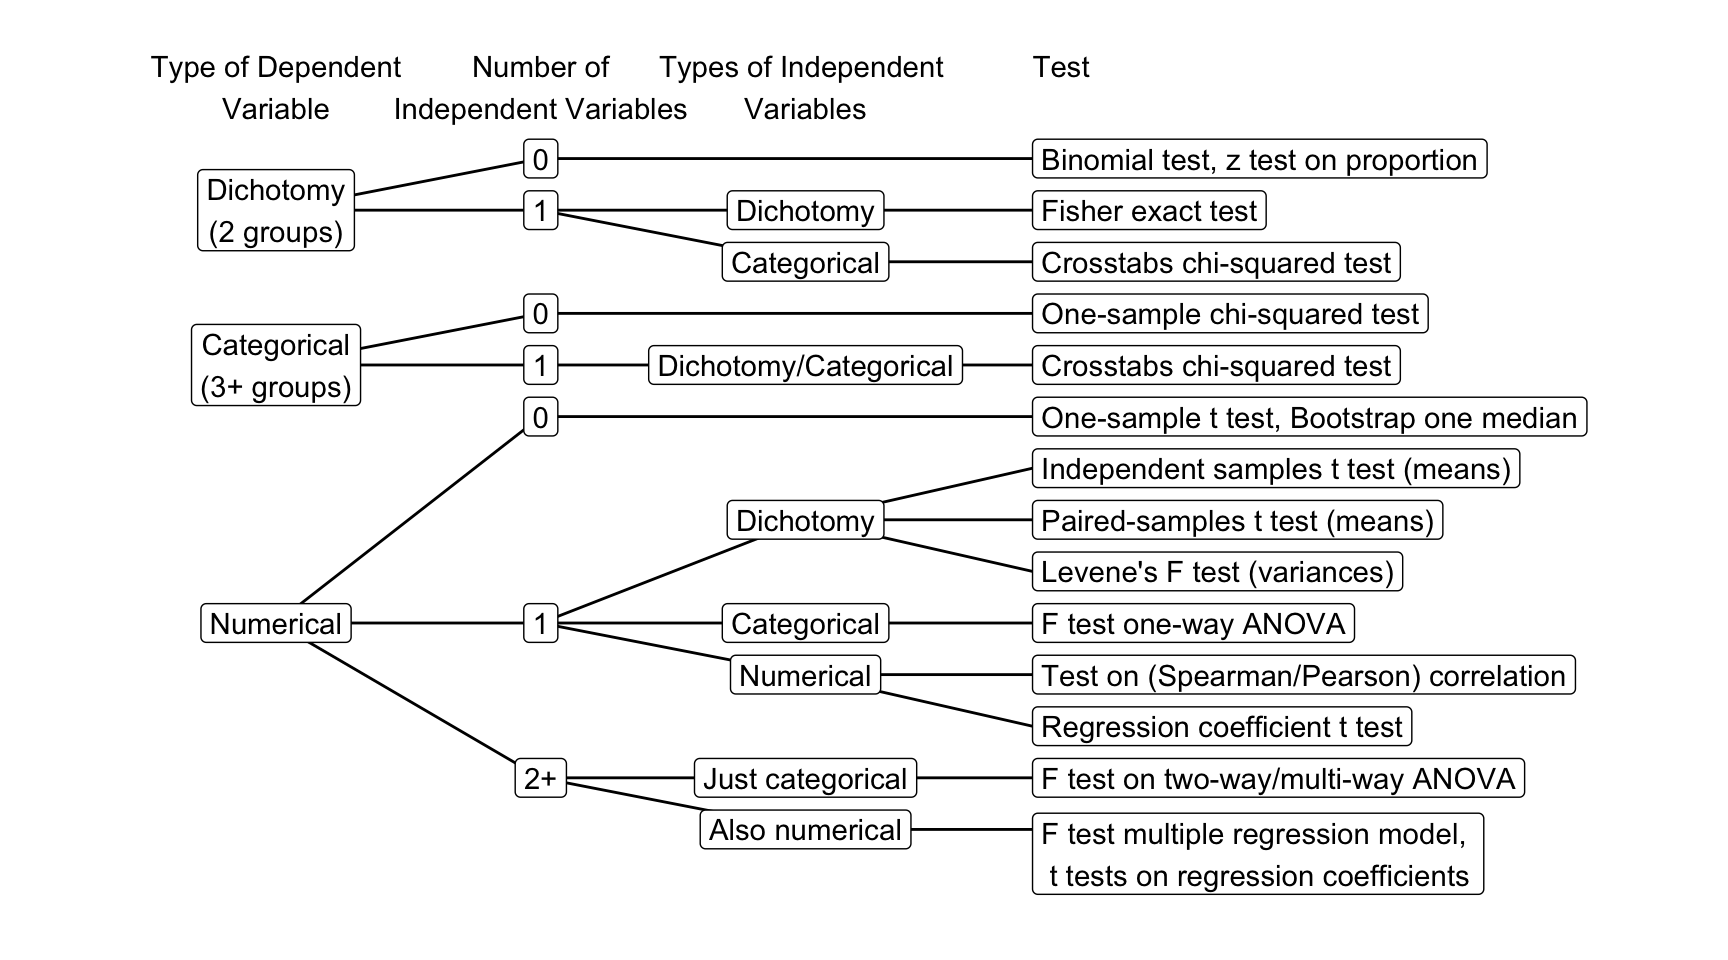
\includegraphics{GentleIntro_files/figure-latex/flowchart-1.pdf}
\caption{\label{fig:flowchart}Flow chart for selecting a test in SPSS.}
\end{figure}

Statistics such as means, proportions, variances, and correlations are
calculated on variables. To translate a research hypothesis into a
statistical hypothesis, the researcher has to recognize the dependent
and independent variables addressed by the research hypothesis and their
variable types. The main distinction is between dichotomies (two
groups), categorical (three or more groups), and numerical variables.
Once you have identified the variables, the flow chart in Figure
\ref{fig:flowchart} helps you to identify the right statistical test.

If possible, SPSS uses a theoretical probability distribution to
approximate the sampling distribution. It will select the appropriate
sampling distribution. In some cases, such as a test on a contingency
table with two rows and two columns, SPSS automatically includes an
exact test because the theoretical approximation cannot be relied on.

SPSS does not allow the user to specify the null hypothesis of the test
if the test involves two or more variables, that is, at least one
dependent variable and one independent variable. Here, SPSS uses the nil
hypothesis, assuming that the population value of interest is zero. For
example, SPSS tests the null hypothesis that males and females have the
same average willingness to donate to a charity, that is, the mean
difference is zero, if we apply an independent samples t test.

Imagine that we know from previous research that females tend to score
one point higher on the willingness score than males. It would not be
very interesting to reject the nil hypothesis. Instead, we would like to
test the null hypothesis that the average difference between females and
males is 1.00. We cannot change the null hypothesis of this t test in
SPSS, but we can use the confidence interval to test our null hypothesis
as explained in Section \ref{null-ci0}.

In SPSS, the analyst has to specify the null hypothesis in tests on one
variable, namely tests on one proportion, one mean, or one categorical
variable. The following instructions explain how to do this.

\subsection{Instructions}\label{instructions-2}

A proportion is the statistic best suited to test research hypotheses
addressing the share of a category in the population. The hypothesis
that a television station reaches half of all households in a country
provides an example. All households in the country constitute the
population. The share of the television station is the proportion or
percentage of all households watching this television station.

If we have a data set on households containing a variable indicating
whether or not a household watches the television station, we can test
the research hypothesis. The statistical null hypothesis is that the
proportion of households watching the television station is 0.5 in the
population.

\begin{figure}[H]
\href{https://www.youtube.com/embed/cA0idFxW-J4}{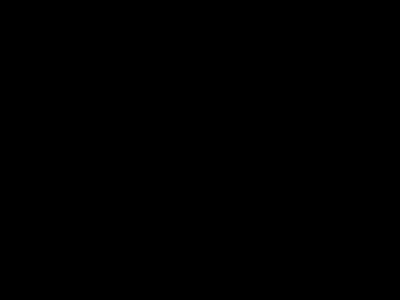
\includegraphics[width=320px]{GentleIntro_files/figure-latex/SPSSbinomial-1} }\caption{A binomial test on a single proportion in SPSS.}\label{fig:SPSSbinomial}
\end{figure}

We can also be interested in more than one category, for instance, in
which regions are the households located: in the north, east, south, and
west of the country? This translates into a statistical hypothesis
containing two or more proportions in the population. If 30\% of
households in the population are situated in the west, 25 \% in the
south and east, and 20\% in the north, we would expect these proportions
in the sample if all regions are equally represented. Our statistical
hypothesis is actually a relative frequency distribution, such as, for
instance, in Table \ref{tab:hypo-freq}.

\begin{table}

\caption{\label{tab:hypo-freq}Statistical hypothesis about four proportions as a frequency table.}
\centering
\fontsize{8}{8}\selectfont
\begin{tabular}[t]{lc}
\hline
Region & Hypothesized Proportion\\
\hline
North & 0.20\\
East & 0.25\\
South & 0.25\\
West & 0.30\\
\hline
\end{tabular}
\end{table}

A test for this type of statistical hypothesis is called a one-sample
chi-squared test. It is up to the researcher to specify the hypothesized
proportions for all categories. This is not a simple task: What reasons
do you have to expect particular values, say a region's share of thirty
per cent of all households instead of twenty-five per cent?

The test is mainly used if the researcher knows the true proportions of
the categories in the population. If we draw a sample from all citizens
of a country, we usually know the frequency distribution of sex, age,
educational level, and so on of all citizens from the national bureau of
statistics. With the bureau's information, we can test if the
respondents in our sample have the same distribution with respect to
sex, age, or educational level as the population; just use the official
population proportions in the hypothesis.

If the proportions in the sample have the same distribution as in the
population, the sample is \emph{representative} (see Section
\ref{representative}) of the population with respect to sex, age, or
educational level. This is an important check on the representativeness
of our sample.

\begin{figure}[H]
\href{https://www.youtube.com/embed/S8I5o_3p6ro}{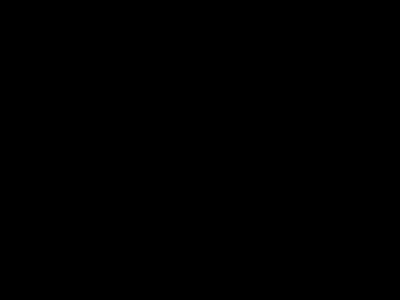
\includegraphics[width=320px]{GentleIntro_files/figure-latex/SPSSchisq1-1} }\caption{A chi-squared test on a frequency distribution in SPSS.}\label{fig:SPSSchisq1}
\end{figure}

Finally, we have the significance test on one mean, which we have used
in the example of average media literacy throughout this chapter. For a
numeric (interval or ratio measurement level) variable such as the
10-point scale in this example, the mean is a good measure of the
distribution's center. Our statistical hypothesis would be that average
media literacy score of all children in the population is (below) 5.5.

\begin{figure}[H]
\href{https://www.youtube.com/embed/Bx0eiqfVfaw}{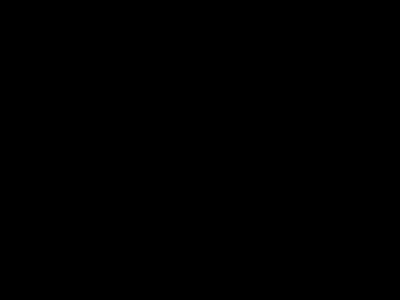
\includegraphics[width=320px]{GentleIntro_files/figure-latex/SPSS1mean-1} }\caption{A one-sample t test in SPSS.}\label{fig:SPSS1mean}
\end{figure}

\subsection{Exercises}\label{exercises-3}

\begin{enumerate}
\def\labelenumi{\arabic{enumi}.}
\tightlist
\item
  Use the data set
  \href{http://82.196.4.233:3838/data/households.sav}{households.sav} to
  test the hypothesis that the TV station does not reach 40 per cent of
  all households in the population.
\end{enumerate}

\begin{Shaded}
\begin{Highlighting}[]
\NormalTok{SPSS syntax}\OperatorTok{:}\StringTok{  }
\StringTok{  }
\ErrorTok{*}\StringTok{ }\NormalTok{Check data.  }
\NormalTok{FREQUENCIES VARIABLES=tv_reach  }
  \OperatorTok{/}\NormalTok{ORDER=ANALYSIS.  }
\OperatorTok{*}\StringTok{ }\NormalTok{Binomial test.  }
\OperatorTok{*}\StringTok{ }\NormalTok{Note}\OperatorTok{:}\StringTok{ }\NormalTok{The test is one}\OperatorTok{-}\NormalTok{sided }\ControlFlowTok{if}\NormalTok{ the test proportion is not }\FloatTok{0.50}\NormalTok{.  }
\NormalTok{NPAR TESTS  }
  \OperatorTok{/}\KeywordTok{BINOMIAL}\NormalTok{ (}\FloatTok{0.40}\NormalTok{)=tv_reach  }
  \OperatorTok{/}\NormalTok{MISSING ANALYSIS.  }
  
\NormalTok{Check data }\OperatorTok{&}\StringTok{ }\NormalTok{assumptions}\OperatorTok{:}\StringTok{   }
\StringTok{  }
\NormalTok{Variable tv_reach is a dichotomy as it should be }\ControlFlowTok{for}\NormalTok{ this test.  }
    
\NormalTok{Interpret the results}\OperatorTok{:}\StringTok{  }
\StringTok{  }
\NormalTok{The proportion of households not reached }\ControlFlowTok{in}\NormalTok{ the }\KeywordTok{sample}\NormalTok{ (}\DataTypeTok{p =} \FloatTok{0.48}\NormalTok{) is above}
\NormalTok{fourty per cent. We have to reject the null hypothesis that the TV station}
\NormalTok{reaches at most fourty per cent of all households, p =}\StringTok{ }\NormalTok{.}\DecValTok{039}\NormalTok{ (one}\OperatorTok{-}\NormalTok{sided).}

\NormalTok{Note that SPSS applies a two}\OperatorTok{-}\NormalTok{sided test }\ControlFlowTok{if}\NormalTok{ the proportion }\ControlFlowTok{in}\NormalTok{ the null}
\NormalTok{hypothesis is .}\DecValTok{50}\NormalTok{, but it applies a one}\OperatorTok{-}\NormalTok{sided test }\ControlFlowTok{in}\NormalTok{ all other situations.}
\NormalTok{This is a left}\OperatorTok{-}\NormalTok{sided test }\ControlFlowTok{if}\NormalTok{ the sample proportion is smaller than the}
\NormalTok{hypothesized proportion and it is a right}\OperatorTok{-}\NormalTok{sided test }\ControlFlowTok{if}\NormalTok{ the sample proportion}
\NormalTok{is larger than the hypothesized proportion.}

\NormalTok{If we translate }\StringTok{"the TV station does not reach 40 per cent of all households in}
\StringTok{the population"}\NormalTok{ into the null hypothesis that the TV station reaches }\DecValTok{40}\NormalTok{ per}
\NormalTok{cent, we need a two}\OperatorTok{-}\NormalTok{sided test. The two}\OperatorTok{-}\NormalTok{sided p value is twice the one}\OperatorTok{-}\NormalTok{sided p}
\NormalTok{value, so the two}\OperatorTok{-}\NormalTok{sided p value would be .}\DecValTok{078}\NormalTok{, which is not significant at the}
\NormalTok{.}\DecValTok{05}\NormalTok{ level.}

\NormalTok{If we translate }\StringTok{"the TV station does not reach 40 per cent of all households in}
\StringTok{the population"}\NormalTok{ into the null hypothesis that the TV station reaches at least}
\DecValTok{40}\NormalTok{ per cent, we need a left}\OperatorTok{-}\NormalTok{sided test. We only reject the null hypothesis }\ControlFlowTok{if}
\NormalTok{our sample proportion is well below the hypothesized value. The left}\OperatorTok{-}\NormalTok{sided test}
\NormalTok{can never be statistically significant }\ControlFlowTok{if}\NormalTok{ the sample proportion is higher than}
\NormalTok{the hypothesized value. This is the case, here}\OperatorTok{:}\StringTok{ }\NormalTok{We hypothesize that the}
\NormalTok{proportion is .}\DecValTok{40} \ControlFlowTok{in}\NormalTok{ the population but the sample proportion is .}\DecValTok{48}\NormalTok{.}
\end{Highlighting}
\end{Shaded}

\begin{enumerate}
\def\labelenumi{\arabic{enumi}.}
\setcounter{enumi}{1}
\tightlist
\item
  Test the hypothesis that the TV station reaches 55 per cent of all
  households in the population.
\end{enumerate}

\begin{Shaded}
\begin{Highlighting}[]
\NormalTok{SPSS syntax}\OperatorTok{:}\StringTok{  }
\StringTok{  }
\ErrorTok{*}\StringTok{ }\NormalTok{Check data.  }
\NormalTok{FREQUENCIES VARIABLES=tv_reach  }
  \OperatorTok{/}\NormalTok{ORDER=ANALYSIS.  }
\OperatorTok{*}\StringTok{ }\NormalTok{Binomial test.  }
\OperatorTok{*}\StringTok{ }\NormalTok{Hint}\OperatorTok{:}\StringTok{ }\NormalTok{Test the proportion of households not reached because   }
\NormalTok{  this is the first category}\OperatorTok{:}\StringTok{ }\DecValTok{1} \OperatorTok{-}\StringTok{ }\FloatTok{0.55}\NormalTok{ =}\StringTok{ }\FloatTok{0.45}\NormalTok{.  }
\NormalTok{NPAR TESTS  }
  \OperatorTok{/}\KeywordTok{BINOMIAL}\NormalTok{ (}\FloatTok{0.45}\NormalTok{)=tv_reach  }
  \OperatorTok{/}\NormalTok{MISSING ANALYSIS.  }
  
\NormalTok{Check data }\OperatorTok{&}\StringTok{ }\NormalTok{assumptions}\OperatorTok{:}\StringTok{   }
\StringTok{  }
\NormalTok{Variable tv_reach is a dichotomy as it should be }\ControlFlowTok{for}\NormalTok{ this test.  }
    
\NormalTok{Interpret the results}\OperatorTok{:}\StringTok{  }
\StringTok{  }
\NormalTok{With }\DecValTok{52}\NormalTok{ per cent of all households reached }\ControlFlowTok{in}\NormalTok{ the sample, we cannot reject the}
\NormalTok{null hypothesis that the TV station reaches at least }\DecValTok{55}\NormalTok{ per cent of all}
\NormalTok{households, p =}\StringTok{ }\NormalTok{.}\DecValTok{260}\NormalTok{ (one}\OperatorTok{-}\NormalTok{sided).}
\end{Highlighting}
\end{Shaded}

\begin{enumerate}
\def\labelenumi{\arabic{enumi}.}
\setcounter{enumi}{2}
\tightlist
\item
  Does half of the households have an income of at most 40,000?
\end{enumerate}

\begin{Shaded}
\begin{Highlighting}[]
\NormalTok{SPSS syntax}\OperatorTok{:}\StringTok{  }
\StringTok{  }
\ErrorTok{*}\StringTok{ }\NormalTok{Check data.  }
\NormalTok{FREQUENCIES VARIABLES=income  }
  \OperatorTok{/}\NormalTok{ORDER=ANALYSIS.  }
\OperatorTok{*}\StringTok{ }\NormalTok{Binomial test.  }
\OperatorTok{*}\StringTok{ }\NormalTok{Use the cut off option }\ControlFlowTok{in}\NormalTok{ the binomial test.  }
\NormalTok{NPAR TESTS  }
  \OperatorTok{/}\KeywordTok{BINOMIAL}\NormalTok{ (}\FloatTok{0.50}\NormalTok{)=}\KeywordTok{income}\NormalTok{ (}\DecValTok{40000}\NormalTok{)  }
  \OperatorTok{/}\NormalTok{MISSING ANALYSIS.  }
  
\NormalTok{Check data}\OperatorTok{:}\StringTok{  }
\StringTok{  }
\ErrorTok{*}\StringTok{ }\NormalTok{There are no apparent impossible income values.  }
  
\NormalTok{Check assumptions}\OperatorTok{:}\StringTok{  }
\StringTok{  }
\NormalTok{There are no assumptions }\ControlFlowTok{for}\NormalTok{ the binomial test.  }
  
\NormalTok{Interpret the results}\OperatorTok{:}\StringTok{  }
\StringTok{  }
\NormalTok{The proportion of households with an income of at most }\DecValTok{40}\NormalTok{,}\DecValTok{000}   
\NormalTok{is significantly less than fifty per cent, p =}\StringTok{ }\NormalTok{.}\DecValTok{022}\NormalTok{. It is   }
\DecValTok{39}\NormalTok{ per cent }\ControlFlowTok{in}\NormalTok{ the sample.  }
\end{Highlighting}
\end{Shaded}

\begin{enumerate}
\def\labelenumi{\arabic{enumi}.}
\setcounter{enumi}{3}
\tightlist
\item
  According to information from the National Bureau of Statistics, 20
  per cent of all households have incomes up to 30,000, 50 per cent have
  incomes between 30,000 and 50,000, and 30 per cent has incomes over
  50,000. Use a test to decide if our sample is representative with
  respect to income. Hint: recode income first.
\end{enumerate}

\begin{Shaded}
\begin{Highlighting}[]
\NormalTok{SPSS syntax}\OperatorTok{:}\StringTok{  }
\StringTok{  }
\ErrorTok{*}\StringTok{ }\NormalTok{Check data.  }
\NormalTok{FREQUENCIES VARIABLES=income  }
  \OperatorTok{/}\NormalTok{ORDER=ANALYSIS.  }
\OperatorTok{*}\StringTok{ }\NormalTok{Recoding income into groups.  }
\NormalTok{RECODE }\KeywordTok{income}\NormalTok{ (Lowest thru }\DecValTok{30000}\NormalTok{=}\DecValTok{1}\NormalTok{) (}\DecValTok{30000}\NormalTok{  thru }\DecValTok{50000}\NormalTok{=}\DecValTok{2}\NormalTok{)  }
\NormalTok{  (}\DecValTok{50000}\NormalTok{ thru }\DataTypeTok{Highest=}\DecValTok{3}\NormalTok{) INTO income_group.  }
\NormalTok{VARIABLE LABELS  income_group }\StringTok{'Grouped income'}\NormalTok{.  }
\NormalTok{EXECUTE.  }
\OperatorTok{*}\StringTok{ }\NormalTok{Define Variable Properties.  }
\OperatorTok{*}\NormalTok{income_group.  }
\NormalTok{VALUE LABELS income_group  }
  \FloatTok{1.00} \StringTok{'low'}  
  \FloatTok{2.00} \StringTok{'medium'}  
  \FloatTok{3.00} \StringTok{'high'}\NormalTok{.  }
\NormalTok{EXECUTE.  }
\OperatorTok{*}\StringTok{ }\NormalTok{one}\OperatorTok{-}\NormalTok{sample chi}\OperatorTok{-}\NormalTok{squared test.  }
\NormalTok{NPAR TESTS  }
  \OperatorTok{/}\NormalTok{CHISQUARE=income_group  }
  \OperatorTok{/}\NormalTok{EXPECTED=}\DecValTok{20} \DecValTok{50} \DecValTok{30}  
  \OperatorTok{/}\NormalTok{MISSING ANALYSIS.  }
  
\NormalTok{There are no apparent impossible income values.  }
  
\NormalTok{Check assumptions}\OperatorTok{:}\StringTok{  }
\StringTok{  }
\NormalTok{Assumptions }\ControlFlowTok{for}\NormalTok{ the chi}\OperatorTok{-}\NormalTok{squared test}\OperatorTok{:}

\ErrorTok{*}\StringTok{ }\NormalTok{Expected frequencies never below }\DecValTok{1}\NormalTok{ and max }\DecValTok{20}\NormalTok{% below }\DecValTok{5}\OperatorTok{:}\StringTok{ }\NormalTok{OK, the SPSS table}
\NormalTok{note says}\OperatorTok{:}\StringTok{ "0 cells (0.0%) have expected frequencies less than 5. The minimum}
\StringTok{expected cell frequency is 24.0."}
\OperatorTok{*}\StringTok{ }\NormalTok{In this case, }\DecValTok{0}\NormalTok{% of the cells have expected frequencies below }\DecValTok{5}\NormalTok{, which is}
\NormalTok{less than the allowed maximum of }\DecValTok{20}\OperatorTok\StringTok{ }\NormalTok{of the}
\NormalTok{cells have expected frequencies of }\DecValTok{5}\NormalTok{ or more.}
   
\NormalTok{Interpret the results}\OperatorTok{:}\StringTok{  }
\StringTok{  }
\NormalTok{The distribution of incomes over income groups }\ControlFlowTok{in}\NormalTok{ the sample does not differ}
\ControlFlowTok{in}\NormalTok{ a statistically significant way from the distribution }\ControlFlowTok{in}\NormalTok{ the population}
\NormalTok{according to the National Bureau of Statistics, chi}\OperatorTok{-}\KeywordTok{squared}\NormalTok{ (}\DecValTok{2}\NormalTok{) =}\StringTok{ }\FloatTok{3.40}\NormalTok{, p =}
\NormalTok{.}\DecValTok{182}\NormalTok{.}
\NormalTok{In other words, we have no reason to believe that our sample is not}
\NormalTok{representative of the population with regards to income.}
\end{Highlighting}
\end{Shaded}

\begin{enumerate}
\def\labelenumi{\arabic{enumi}.}
\setcounter{enumi}{4}
\tightlist
\item
  Use the data set
  \href{http://82.196.4.233:3838/data/children.sav}{children.sav} to
  test the hypothesis that average parental supervision of the child's
  media use is 5.5 (on a scale from 1 to 10) in the population.
\end{enumerate}

\begin{Shaded}
\begin{Highlighting}[]
\NormalTok{SPSS syntax}\OperatorTok{:}\StringTok{  }
\StringTok{  }
\ErrorTok{*}\StringTok{ }\NormalTok{Check data.  }
\NormalTok{FREQUENCIES VARIABLES=supervision  }
  \OperatorTok{/}\NormalTok{ORDER=ANALYSIS.  }
\OperatorTok{*}\StringTok{ }\NormalTok{Set imposible }\KeywordTok{value}\NormalTok{ (}\DecValTok{25}\NormalTok{) to missing.  }
\OperatorTok{*}\StringTok{ }\NormalTok{Define Variable Properties.  }
\OperatorTok{*}\NormalTok{supervision.  }
\NormalTok{MISSING VALUES }\KeywordTok{supervision}\NormalTok{(}\FloatTok{25.00}\NormalTok{).  }
\NormalTok{EXECUTE.  }
\OperatorTok{*}\StringTok{ }\NormalTok{One}\OperatorTok{-}\NormalTok{sample t test.  }
\NormalTok{T}\OperatorTok{-}\NormalTok{TEST  }
  \OperatorTok{/}\NormalTok{TESTVAL=}\FloatTok{5.5}  
  \OperatorTok{/}\NormalTok{MISSING=ANALYSIS  }
  \OperatorTok{/}\NormalTok{VARIABLES=supervision  }
  \OperatorTok{/}\NormalTok{CRITERIA=}\KeywordTok{CI}\NormalTok{(.}\DecValTok{95}\NormalTok{).  }
  
\NormalTok{Check data}\OperatorTok{:}\StringTok{  }
\StringTok{      }
\NormalTok{There is one impossible value }\ControlFlowTok{for}\NormalTok{ parental supervision,  }
\NormalTok{namely }\DecValTok{25}\NormalTok{. This value must be made missing.  }
  
\NormalTok{Check assumptions}\OperatorTok{:}\StringTok{  }
\StringTok{  }
\NormalTok{Sample }\KeywordTok{size}\NormalTok{ (}\DataTypeTok{N =} \DecValTok{86}\NormalTok{) is well over }\DecValTok{30}\NormalTok{, so we need not worry  }
\NormalTok{about the shape of the variable distribution }\ControlFlowTok{in}\NormalTok{ the  }
\NormalTok{population.  }
    
\NormalTok{Interpret the results}\OperatorTok{:}\StringTok{  }
\StringTok{  }
\NormalTok{In the sample, average parental supervision is }\FloatTok{5.36}\NormalTok{ (}\DataTypeTok{SD =} \FloatTok{1.94}\NormalTok{) on a scale}
\NormalTok{from }\DecValTok{1}\NormalTok{ to }\DecValTok{10}\NormalTok{. We are rather confident that the true average supervision score}
\ControlFlowTok{in}\NormalTok{ the population is around }\FloatTok{5.5}\NormalTok{, more specifically, between }\FloatTok{4.94}\NormalTok{ and }\FloatTok{5.77}\NormalTok{. A}
\NormalTok{test is not statistically significant, }\KeywordTok{t}\NormalTok{ (}\DecValTok{85}\NormalTok{) =}\StringTok{ }\OperatorTok{-}\FloatTok{0.68}\NormalTok{, p =}\StringTok{ }\NormalTok{.}\DecValTok{498}\NormalTok{, }\DecValTok{95}\NormalTok{%CI[}\FloatTok{4.94}\NormalTok{;}
\FloatTok{5.77}\NormalTok{].}
  
\NormalTok{Note that we have to add the confidence interval limits to the test value}
\NormalTok{(here}\OperatorTok{:}\StringTok{ }\FloatTok{5.5}\NormalTok{) to obtain the confidence interval }\ControlFlowTok{for}\NormalTok{ the population mean. SPSS}
\NormalTok{reports the confidence interval }\ControlFlowTok{for}\NormalTok{ the difference between the hypothesized}
\NormalTok{population mean and the sample mean.}
\end{Highlighting}
\end{Shaded}

\begin{enumerate}
\def\labelenumi{\arabic{enumi}.}
\setcounter{enumi}{5}
\tightlist
\item
  If you would test the hypothesis that average parental supervision in
  the population is 4.5, would the test be statistically significant
  according to the confidence interval reported for Exercise 5? Check
  your answer by carrying out the test.
\end{enumerate}

\begin{Shaded}
\begin{Highlighting}[]
\NormalTok{The confidence interval reported }\ControlFlowTok{in}\NormalTok{ Exercise }\DecValTok{5}\NormalTok{ is }\DecValTok{95}\NormalTok{%CI[}\FloatTok{4.94}\NormalTok{; }\FloatTok{5.77}\NormalTok{].}
\NormalTok{It tells us that all null hypotheses with a hypothesized population mean}
\NormalTok{between }\FloatTok{4.94}\NormalTok{ and }\FloatTok{5.77}\NormalTok{ would NOT be rejected with the current sample. All}
\NormalTok{hypotheses with population values outside this confidence interval would be}
\NormalTok{rejected by the current sample }\ControlFlowTok{in}\NormalTok{ a two}\OperatorTok{-}\NormalTok{sided test with five per cent}
\NormalTok{significance level.}
\NormalTok{The null hypothesis that average parental supervision }\ControlFlowTok{in}\NormalTok{ the population is }\FloatTok{4.5}
\NormalTok{is outside the confidence interval, so it would be rejected by the current}
\NormalTok{sample. A test with this null hypothesis would be statistically significant.}
\NormalTok{We can check this be executing the test. But note that this is only a check; we}
\NormalTok{already know the result.}

\NormalTok{SPSS syntax}\OperatorTok{:}\StringTok{  }
\StringTok{  }
\ErrorTok{*}\StringTok{ }\NormalTok{Check data.  }
\NormalTok{FREQUENCIES VARIABLES=supervision  }
  \OperatorTok{/}\NormalTok{ORDER=ANALYSIS.  }
\OperatorTok{*}\StringTok{ }\NormalTok{Set imposible }\KeywordTok{value}\NormalTok{ (}\DecValTok{25}\NormalTok{) to missing.  }
\OperatorTok{*}\StringTok{ }\NormalTok{Define Variable Properties.  }
\OperatorTok{*}\NormalTok{supervision.  }
\NormalTok{MISSING VALUES }\KeywordTok{supervision}\NormalTok{(}\FloatTok{25.00}\NormalTok{).  }
\NormalTok{EXECUTE.  }
\OperatorTok{*}\StringTok{ }\NormalTok{One}\OperatorTok{-}\NormalTok{sample t test.  }
\NormalTok{T}\OperatorTok{-}\NormalTok{TEST  }
  \OperatorTok{/}\NormalTok{TESTVAL=}\FloatTok{4.5}  
  \OperatorTok{/}\NormalTok{MISSING=ANALYSIS  }
  \OperatorTok{/}\NormalTok{VARIABLES=supervision  }
  \OperatorTok{/}\NormalTok{CRITERIA=}\KeywordTok{CI}\NormalTok{(.}\DecValTok{95}\NormalTok{).  }
  
\NormalTok{Check data}\OperatorTok{:}\StringTok{  }
\StringTok{  }
\NormalTok{There is one impossible value }\ControlFlowTok{for}\NormalTok{ parental supervision,  }
\NormalTok{namely }\DecValTok{25}\NormalTok{. This value must be made missing.  }
  
\NormalTok{Check assumptions}\OperatorTok{:}\StringTok{  }
\StringTok{  }
\NormalTok{Sample }\KeywordTok{size}\NormalTok{ (}\DataTypeTok{N =} \DecValTok{86}\NormalTok{) is well over }\DecValTok{30}\NormalTok{, so we need not worry  }
\NormalTok{about the shape of the variable distribution }\ControlFlowTok{in}\NormalTok{ the  }
\NormalTok{population.  }
  
\NormalTok{Interpret the results}\OperatorTok{:}\StringTok{  }
\StringTok{  }
\NormalTok{The average parental supervision score }\ControlFlowTok{in}\NormalTok{ the sample   }
\NormalTok{(}\DataTypeTok{M =} \FloatTok{5.36}\NormalTok{, }\DataTypeTok{SD =} \FloatTok{1.94}\NormalTok{) makes us doubt that the true  }
\NormalTok{average supervision score }\ControlFlowTok{in}\NormalTok{ the population is }\FloatTok{4.5}\NormalTok{ or  }
\NormalTok{thereabouts, }\KeywordTok{t}\NormalTok{ (}\DecValTok{85}\NormalTok{) =}\StringTok{ }\FloatTok{4.10}\NormalTok{, p }\OperatorTok{<}\StringTok{ }\NormalTok{.}\DecValTok{001}\NormalTok{, }\DecValTok{95}\NormalTok{%CI[}\FloatTok{4.94}\NormalTok{; }\FloatTok{5.77}\NormalTok{].  }
  
\NormalTok{Note that we obtain the same confidence interval as }\ControlFlowTok{in}  
\NormalTok{Exercise }\DecValTok{1}\NormalTok{. The confidence interval does not depend on   }
\NormalTok{the null hypothesis, whereas the significance test does.  }
\end{Highlighting}
\end{Shaded}

\section{Capitalization on Chance}\label{cap-chance}

The relation between null hypothesis testing and confidence intervals
(Section \ref{null-ci0}) may have given the impression that we can test
a range of null hypotheses using just one sample and one confidence
interval. For instance, we could simultaneously test the null hypotheses
that average media literacy among children is 5.5, 4.5, or 3.5. Just
check if these values are inside or outside the confidence interval and
we are done, right?

This impression is wrong. The probabilities that we calculate using one
sample assume that we only apply one test to the data. If we test the
original null hypothesis that average media literacy is 5.5, we run a
risk of five per cent to reject the null hypothesis if the null
hypothesis is true. The significance level is the probability of making
a Type I error (Section \ref{sig-typeI}).

If we apply a second test to the same sample, for example, testing the
null hypothesis that average media literacy is 4.5, we again run this
risk of five per cent. The probability of not rejecting a true null
hypothesis is .95, so the probability of not rejecting two true null
hypotheses is .95 * .95 = 0.9025. The risk of rejecting at least one
true null hypothesis in two tests is 1 - 0.9025 = .0975. This risk is
dramatically higher than the significance level (.05) that we want to
use. The situation becomes even worse if we do three or more tests on
the same sample.

The phenomenon that we are dealing with probabilities of making Type I
errors that are higher (\emph{inflated Type I errors}) than the
significance level that we want to use, is referred to as
\emph{capitalization on chance}. Applying more than one test to the same
data is one way to capitalize on chance. If you do a lot of tests on the
same data, it is very rare not to find some statistically significant
results even if all null hypotheses are true.

\subsection{Capitalization on chance in post-hoc
tests}\label{capitalization-on-chance-in-post-hoc-tests}

This type of capitalization on chance may occur, for example, in an
analysis of variance. To test the research hypothesis that the celebrity
endorsing a fundraising campaign makes a difference to people's
willingness to donate, we may organize an experiment using three
versions of a video clip as the treatment, each clip featuring a
different celebrity endorsing the campaign. This results in three groups
of participants, each group having an average score on their willingness
to donate. As a first step, we test the null hypothesis that all groups
have equal population means using an \emph{F} test (analysis of
variance).

If this test is statistically significant, we reject the null hypothesis
and conclude that at least two groups have different population means.
The next question is: Which groups, that is, endorsement by which
celebrities, display a different willingness to donate? To answer this
question, we must do post-hoc \emph{t} tests on pairs of groups. With
three groups (A, B, and C), we have three pairs of groups (AB, AC, and
BC), so we have three \emph{t} tests on independent means. The
probability of rejecting at least one true null hypothesis of no
difference is much higher than five per cent if we use a significance
level of five per cent for each single \emph{t} test.

\subsection{Correcting for capitalization on
chance}\label{correcting-for-capitalization-on-chance}

We can correct in several ways for this type of capitalization on
chance; one such way is by applying the Bonferroni correction. This
correction merely divides the significance level that we use for each
test by the number of tests that we do. In our example, we do three
\emph{t} tests on pairs of groups, so we divide the significance level
of five per cent by three. The resulting significance level for each
\emph{t} test is .0167. If a \emph{t} test's p value is below .0167, we
reject the null hypothesis, but we do not reject it otherwise.

The Bonferroni correction is a rather coarse correction, which is not
entirely accurate. However, it has a simple logic that directly links to
the problem of capitalization on chance. Therefore, it is a good
technique to help understand the problem, which is the main goal we want
to attain, here. We will skip better, but more complicated alternatives
to Bonferroni correction.

Note that we need not apply a correction if we specify a hypothesis
beforehand about the two groups that we expect to differ. In the example
of celebrity endorsement, we would not have to apply the Bonferroni
correction to the \emph{t} test on the mean difference between
participants confronted to Celebrity A and Celebrity C if we had
hypothesized that the willingness to donate differs here. Of course, we
could have skipped the analysis of variance and gone straight to the
\emph{t} test with such a hypothesis.

\subsection{Specifying hypotheses
afterwards}\label{specifying-hypotheses-afterwards}

Capitalization on chance occurs if we apply different tests to the same
variables in the same sample. This occurs in exploratory research in
which we do not specify hypotheses beforehand but try out different
independent variables or different dependent variables.

It occurs more strongly if we first have a look at our sample data and
then formulate the hypothesis. Knowing the sample outcome, it is easy to
specify a null hypothesis that will be rejected. This is plain cheating
and it must be avoided at all times.

\section{Test Your Understanding}\label{test-your-understanding-3}

\begin{figure}[H]
\href{http://82.196.4.233:3838/apps/null-ci/}{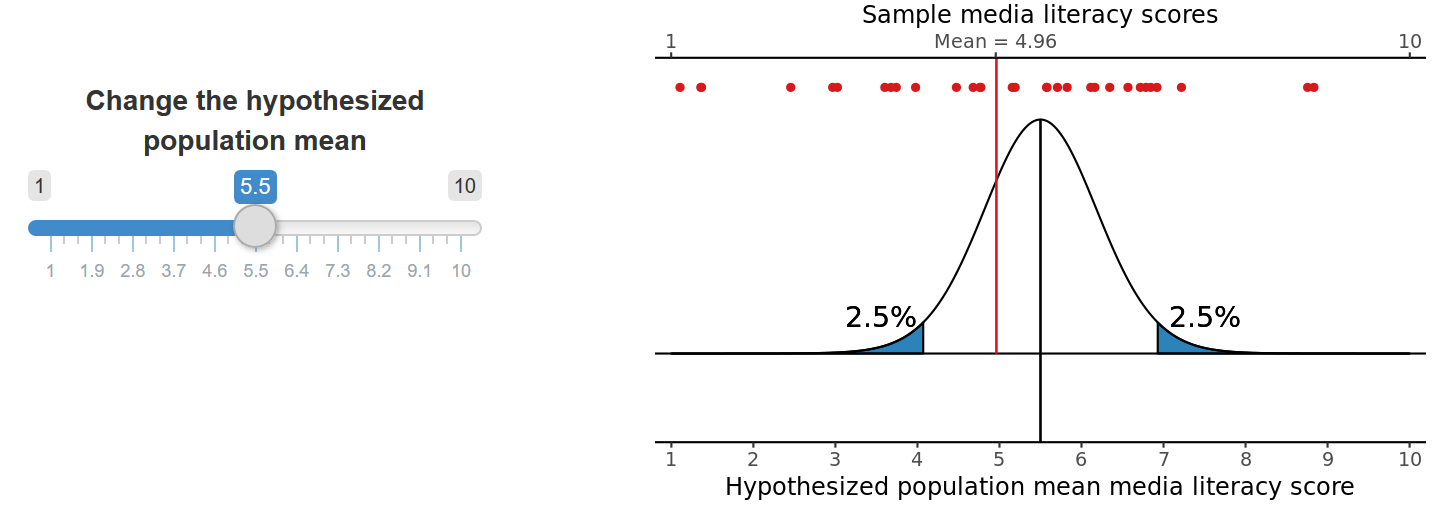
\includegraphics[width=420px]{GentleIntro_files/figure-latex/hypo-testing-1} }\caption{Testing null hypotheses.}\label{fig:hypo-testing}
\end{figure}

Figure \ref{fig:hypo-testing} displays a random sample of media literacy
scores (red) and a sampling distribution if the null hypothesis is true.

\begin{enumerate}
\def\labelenumi{\arabic{enumi}.}
\tightlist
\item
  What are the null and alternative hypotheses in Figure
  \ref{fig:hypo-testing}? Is the null hypothesis a nil hypothesis here?
\end{enumerate}

\begin{Shaded}
\begin{Highlighting}[]
\OperatorTok{*}\StringTok{ }\NormalTok{The null hypothesis is that average media literacy}
\NormalTok{score }\ControlFlowTok{in}\NormalTok{ the population is }\FloatTok{5.5}\NormalTok{. This is not a nil}
\NormalTok{hypothesis because the hypothesized value is not zero.}
\OperatorTok{*}\StringTok{ }\NormalTok{The significance level is split between the two tails}
\NormalTok{of the sampling distribution, so a two}\OperatorTok{-}\NormalTok{sided test is}
\NormalTok{intended. The alternative hypothesis of this two}\OperatorTok{-}\NormalTok{sided}
\NormalTok{significance test is that the population mean is NOT}
\FloatTok{5.5}\NormalTok{; it is either higher or lower than }\FloatTok{5.5}\NormalTok{.}
\end{Highlighting}
\end{Shaded}

\begin{enumerate}
\def\labelenumi{\arabic{enumi}.}
\setcounter{enumi}{1}
\tightlist
\item
  What represents the p value of the sample mean that we have found in
  Figure \ref{fig:hypo-testing}? Does the p value depend on the type of
  null hypothesis: one-sided or two-sided?
\end{enumerate}

\begin{Shaded}
\begin{Highlighting}[]
\OperatorTok{*}\StringTok{ }\NormalTok{The p value of the test is the surface of the tail of the sampling}
\NormalTok{distribution that is further away from the hypothesized value than the sample}
\NormalTok{mean. Graphically speaking, it is the surface of the tail that is cut of by}
\NormalTok{the red line.}
\OperatorTok{*}\StringTok{ }\NormalTok{In a one}\OperatorTok{-}\NormalTok{sided test, the p value is just the surface of this tail. In a}
\NormalTok{two}\OperatorTok{-}\NormalTok{sided test, it is the twice this surface because it also includes the same}
\NormalTok{part of the tail at the other side of the distribution.}
\OperatorTok{*}\StringTok{ }\NormalTok{So yes, it makes a difference to the p value whether you test one}\OperatorTok{-}\NormalTok{sided or}
\NormalTok{two}\OperatorTok{-}\NormalTok{sided.}
\end{Highlighting}
\end{Shaded}

\begin{enumerate}
\def\labelenumi{\arabic{enumi}.}
\setcounter{enumi}{2}
\tightlist
\item
  What part of Figure \ref{fig:hypo-testing} represents the significance
  level and rejection region?
\end{enumerate}

\begin{Shaded}
\begin{Highlighting}[]
\OperatorTok{*}\StringTok{ }\NormalTok{The surface of the blue tails represent the significance level of the test.}
\NormalTok{Each tail contains }\FloatTok{2.5}\OperatorTok\NormalTok{.}
\OperatorTok{*}\StringTok{ }\NormalTok{The rejection region contains the sample statistic values under the blue}
\NormalTok{tails. Graphically speaking, the rejection region consists of the segments of}
\NormalTok{the horizontal axis under the blue tails. These are the sample average media}
\NormalTok{literacy scores that differ too much from the hypothesized population mean to}
\NormalTok{believe that the hypothesized mean is the true population mean.}
\end{Highlighting}
\end{Shaded}

\begin{enumerate}
\def\labelenumi{\arabic{enumi}.}
\setcounter{enumi}{3}
\tightlist
\item
  Is the test statistically significant? How do you decide?
\end{enumerate}

\begin{Shaded}
\begin{Highlighting}[]
\OperatorTok{*}\StringTok{ }\NormalTok{If the sample }\KeywordTok{mean}\NormalTok{ (red line) falls within a blue }\KeywordTok{tail}\NormalTok{ (rejection region)}
\NormalTok{of the sampling distribution, the null hypothesis must be rejected.}
\OperatorTok{*}\StringTok{ }\NormalTok{Note that the blue tails extend infinitely away from the hypothesized value}
\NormalTok{but the density becomes quickly so small that you can not see the blue surface}
\NormalTok{everywhere.}
\end{Highlighting}
\end{Shaded}

\begin{enumerate}
\def\labelenumi{\arabic{enumi}.}
\setcounter{enumi}{4}
\tightlist
\item
  What happens if you change the hypothesized population mean? Check
  your answer by using the slider.
\end{enumerate}

\begin{Shaded}
\begin{Highlighting}[]
\OperatorTok{*}\StringTok{ }\NormalTok{The curve moves horizontally because it represents the sampling distribution}
\ControlFlowTok{if}\NormalTok{ the null hypothesis is true. It assumes that the true population mean is}
\NormalTok{equal to the hypothesized population mean.}
\OperatorTok{*}\StringTok{ }\NormalTok{The population mean is the expected value of the sampling distribution, so}
\NormalTok{it is the centre of this distribution. If we change the hypothesized mean, we}
\NormalTok{change the centre of the distribution, so it moves to the left or right.}
\end{Highlighting}
\end{Shaded}

\begin{enumerate}
\def\labelenumi{\arabic{enumi}.}
\setcounter{enumi}{5}
\tightlist
\item
  Is it OK to change your null hypothesis when you know your sample
  mean? Why is it OK or not OK?
\end{enumerate}

\begin{Shaded}
\begin{Highlighting}[]
\OperatorTok{*}\StringTok{ }\NormalTok{It is NOT OK to change your null hypothesis when you know your sample mean}
\NormalTok{because you can always find a null hypothesis that is statistically}
\NormalTok{significant. Just move you null hypothesis so your sample }\KeywordTok{mean}\NormalTok{ (red) ends up}
\ControlFlowTok{in} \KeywordTok{the}\NormalTok{ (blue) region outside the critical values.}
\OperatorTok{*}\StringTok{ }\NormalTok{You do not offer the data a fair chance to prove that your null hypothesis is}
\NormalTok{wrong }\ControlFlowTok{if} \KeywordTok{you}\NormalTok{ (re)formulate the null hypothesis when you know your sample.}
\OperatorTok{*}\StringTok{ }\NormalTok{This would be an example of capitalization on chance.}
\end{Highlighting}
\end{Shaded}

\section{Take-Home Points}\label{take-home-points-3}

\begin{itemize}
\item
  We use a statistical test if we want to decide on a null hypothesis:
  reject or not reject? Usually, this boils down to the question: Is
  there or is there not an effect (difference, association) in the
  population?
\item
  The decision rules should be specified beforehand: Decide on the
  direction of the test (one-sided or two-sided) and the significance
  level.
\item
  The null and alternative hypotheses always concern a population
  statistic. Together they cover all possible outcomes for the
  statistic. The null hypothesis always specifies one (boundary) value
  for the population statistic.
\item
  We reject the null hypothesis if a test is statistically significant.
  This means that the probability of drawing a sample with the current
  or a more extreme outcome (even more inconsistent with the null
  hypothesis) if the null hypothesis is true (conditional probability)
  is below the significance level.
\item
  The 95\% confidence interval includes all null hypotheses that would
  \emph{not} be rejected in a two-sided test at five per cent
  significance level. It contains the population values that are not
  sufficiently contradicted by the data.
\item
  The calculated p value is only correct if the data is used for no more
  than one null hypothesis test and the null hypothesis was formulated
  beforehand.
\item
  If the same data is used for more null hypotheses tests, the
  probability of a Type I error increases. We obtain too many
  significant results, which is called capitalization on chance.
\end{itemize}

\chapter{Which Sample Size Do I Need? Power!}\label{power}

\begin{quote}
Key concepts: minimum sample size, unstandardized effect size,
practically significant, standardized effect size, Cohen's d for means,
Type I error, Type II error, test power.
\end{quote}

\subsection*{Summary}\label{summary-4}
\addcontentsline{toc}{subsection}{Summary}

\begin{quote}
How large should my sample be?
\end{quote}

At the start of a quantitative research project, we are confronted with
a seemingly simple practical question: How large should our sample be?
In some cases, the statistical test that we plan to use gives us rules
of thumb for the minimum size that we need for this test.

This may tell us the minimum sample size but not necessarily the optimal
sample size. Even if we can apply the statistical test technically,
sample size need not be sufficient for the test to signal the population
differences or associations, for short, the effect sizes, that we are
interested in.

If we want to know the minimum sample size that we need to signal
important effects in our data, things become rather complicated. We have
to decide on the size of effects that we deem interesting. We also have
to decide on the minimum probability that the statistical test will
actually reject the nil hypothesis of no effect if the true effect in
the population is of this size.

This probability is the power of a test: the probability to reject a
null hypothesis of no effect if the effect in the population is of a
size interesting to us. If we do not reject a false null hypothesis, we
make a Type II error.

Thinking about sample size thus confronts us with a problem that we have
hitherto neglected, namely the problem of not rejecting a false null
hypothesis. This problem is very important if the null hypothesis
represents our research hypothesis. If the null hypothesis represents
our research hypothesis, our expectations are confirmed if we do
\emph{not} succeed in rejecting the null hypothesis.

However, if we do \emph{not} reject the null hypothesis, we cannot make
a Type I error, namely rejecting a true null hypothesis. As a
consequence, the significance level of our test, which is the maximum
probability of making a Type I error, is meaningless. We must know the
probability of rejecting a false null hypothesis---the power of the
test---to express our confidence that our research hypothesis is true.

This chapter reviews concepts that are central to understanding what
statistical significance of a test means: sampling distribution,
hypotheses, statistical significance, and Type I error. It adds concepts
needed to interpret a test that is \emph{not} statistically significant:
effect size, practical significance, Type II error, and test power.

\section{Sample Size and Test Requirements}\label{size-test-req}

Table \ref{tab:thumb} in Chapter \ref{probmodels} shows the conditions
that must be satisfied if we want to use a theoretical probability
distribution to approximate a sampling distribution. Only if the
conditions are met, the theoretical probability distribution resembles
the sampling distribution sufficiently for using the former as
approximation of the latter.

\begin{table}[H]

\caption{\label{tab:thumbsize}Rules of thumb for minimum sample sizes.}
\centering
\fontsize{8}{8}\selectfont
\begin{tabular}[t]{p{4cm}p{4cm}p{4cm}}
\hline
Distribution & Sample statistic & Minimum sample size\\
\hline
Binomial distribution & proportion & -\\
(Standard) normal distribution & proportion & >= 5 divided by test proportion (<= .5)\\
(Standard) normal distribution & one or two means & > 100\\
t distribution & one or two means & each group > 30\\
t distribution & (Spearman) rank correlation coefficient & > 30\\
t distribution & regression coefficient & 20+ per independent variable\\
F distribution & 3+ means & all groups are more or less of equal size\\
chi-squared distribution & row or cell frequencies & expected frequency >= 1 and 80\% >= 5\\
\hline
\end{tabular}
\end{table}

Conditions often include sample size. Table \ref{tab:thumbsize}
reproduces the size requirements from Table \ref{tab:thumb}. If you plan
to do a t test, either on its own or in post-hoc tests after analysis of
variance, each group should contain more than thirty cases. So if you
intend to apply t tests, recruit more than thirty participants for each
experimental group or more than thirty respondents for each group in
your survey. If you have to reckon with non-response, that is, sampled
participants or respondents unwilling to participate in your research,
you should recruit more participants or respondents to have more than
thirty observations in the end.

Chi-squared tests require a minimum of five expected frequencies per
category in a frequency distribution or cell in a contingency table.
Your sample size should be at least the number of categories or cells
times five to come even near this requirement. Regression analysis
requires at least 20 cases per independent variable in the regression
model.

The variation of sample size across groups is important to analysis of
variance (ANOVA), which uses the F distribution. If the number of cases
is more or less the same across all groups, we need not worry about the
variances of the dependent variable for the groups in the population. To
be on the safe side, then, it is recommended to design your sampling
strategy in such a way that you end up with more or less equal group
sizes if you plan to use analysis of variance.

\section{Effect Size}\label{effectsize}

\begin{figure}[H]
\href{http://82.196.4.233:3838/apps/sample-size-unstand/}{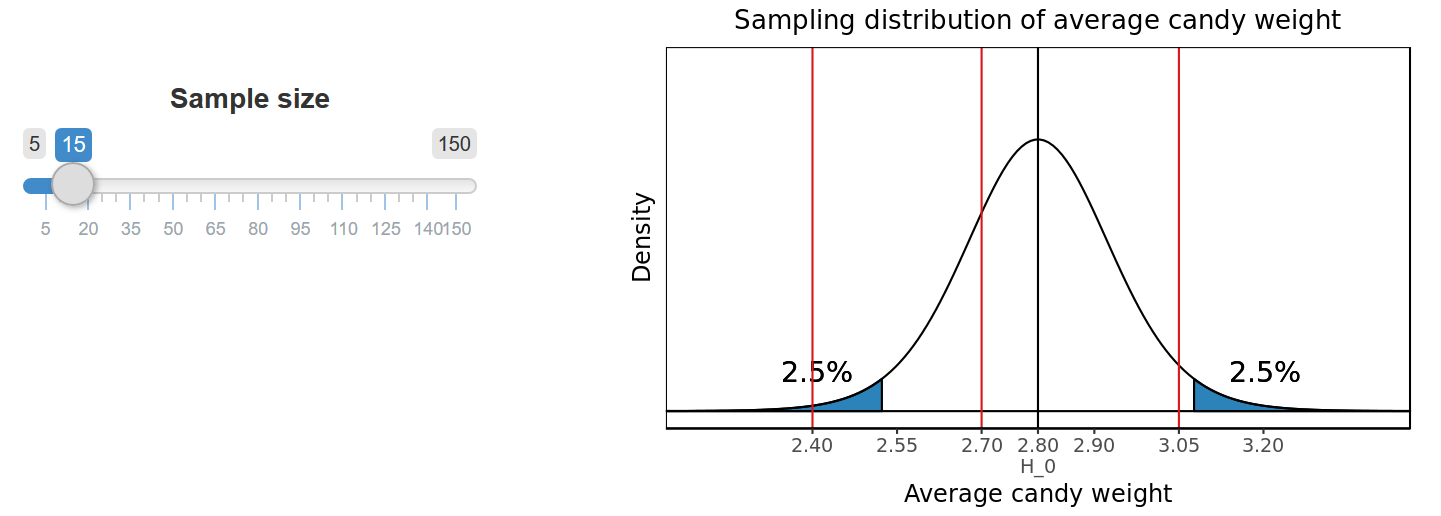
\includegraphics[width=420px]{GentleIntro_files/figure-latex/sample-size-unstand-1} }\caption{Sampling distribution of average candy weight under the null hypothesis that average candy weight is 2.8 gram in the population.}\label{fig:sample-size-unstand}
\end{figure}

\begin{enumerate}
\def\labelenumi{\arabic{enumi}.}
\tightlist
\item
  If we draw a sample of twenty candies, which average candy weight in
  our sample rejects the null hypothesis according to Figure
  \ref{fig:sample-size-unstand}: 2.40, 2.70, or 3.05 gram?
\end{enumerate}

\begin{Shaded}
\begin{Highlighting}[]
\OperatorTok{*}\StringTok{ }\NormalTok{Of the three sample outcomes, a sample with }\FloatTok{2.40}\NormalTok{ gram }\ControlFlowTok{for}\NormalTok{ average candy}
\KeywordTok{weight}\NormalTok{ (red line at the left) is the only sample that is statistically}
\NormalTok{significant With the initial sample }\KeywordTok{size}\NormalTok{ (}\DataTypeTok{N =} \DecValTok{15}\NormalTok{). It is the only weight that}
\NormalTok{crosses a blue tail, which tells us that it is }\ControlFlowTok{in}\NormalTok{ the rejection region of the}
\NormalTok{test.}
\end{Highlighting}
\end{Shaded}

\begin{enumerate}
\def\labelenumi{\arabic{enumi}.}
\setcounter{enumi}{1}
\tightlist
\item
  Imagine that legal regulations allow average candy weight in a sample
  bag to differ 0.10 gram but not 0.25 gram from the weight reported on
  the sample bag. Our statistical test should pick up (be significant)
  differences of at least 0.25 gram, but not differences of 0.10 gram or
  less. How large should our sample be?
\end{enumerate}

\begin{Shaded}
\begin{Highlighting}[]
\OperatorTok{*}\StringTok{ }\NormalTok{Average weight }\ControlFlowTok{in}\NormalTok{ the sample differs }\FloatTok{0.25}\NormalTok{ from the hypothesized }\KeywordTok{value}\NormalTok{ (}\FloatTok{2.80}
\NormalTok{gram) }\ControlFlowTok{for}\NormalTok{ a sample average of }\FloatTok{0.25} \OperatorTok{+}\StringTok{ }\FloatTok{2.80}\NormalTok{ =}\StringTok{ }\FloatTok{3.05}\NormalTok{. This value is marked by the}
\NormalTok{red line at the right.}
\OperatorTok{*}\StringTok{ }\NormalTok{The value }\FloatTok{3.05}\NormalTok{ starts falling within the rejection }\KeywordTok{region}\NormalTok{ (under the blue}
\NormalTok{tails) at sample size }\DecValTok{18}\NormalTok{. This is the minimum sample size we need to get a}
\NormalTok{statistically significant result }\ControlFlowTok{for}\NormalTok{ a sample average that differs }\FloatTok{0.25}\NormalTok{ gram}
\NormalTok{from the hypothesized value.}
\OperatorTok{*}\StringTok{ }\NormalTok{Average sample candy weight of }\FloatTok{2.70}\NormalTok{, which is }\FloatTok{0.10}\NormalTok{ below the hypothesized}
\KeywordTok{value}\NormalTok{ (}\FloatTok{2.80}\NormalTok{), becomes statistically significant at sample size }\DecValTok{91}\NormalTok{. Samples of}
\NormalTok{this size or larger pick up differences that are too small to be of interest to}
\NormalTok{us. Their statistical significance give a false alarm, so to speak.}
\OperatorTok{*}\StringTok{ }\NormalTok{All sample sizes from }\DecValTok{18}\NormalTok{ up to and including }\DecValTok{19}\NormalTok{ serve our purpose, namely}
\NormalTok{signalling differences larger than }\FloatTok{0.10}\NormalTok{ gram and always signalling a difference}
\NormalTok{of }\FloatTok{0.25}\NormalTok{ gram.}
\end{Highlighting}
\end{Shaded}

We have learned that larger samples have smaller standard errors
(Section \ref{sample-size}). Smaller standard errors yield (absolutely)
larger test statistic values and larger test statistics have smaller p
values. In other words, a test on a larger sample is more often
statistically significant.

A larger sample offers more precision, so the difference between our
sample outcome and the hypothesized value is more often sufficient to
reject the null hypothesis. For example, we would reject the null
hypothesis that average candy weight is 2.8 gram in the population if
the average weight in our sample bag is 2.70 gram and our sample is
large. But we may not reject this null hypothesis if we have the same
outcome in a small sample bag.

Of course, the size of the difference between our sample outcome and the
hypothesized population value matters as well. This difference is called
\emph{effect size}. If average candy weight in our sample bag deviates
more from the average weight that we expect according to the null
hypothesis, we are more likely to reject the null hypothesis. If we
think of our statistical test as a security metal detector, our test
will pick up larger amounts of metal more easily.

\begin{figure}[H]
\centering
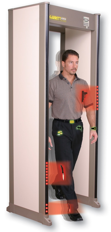
\includegraphics{figures/metaldetector.png}
\caption{Security metal detector}
\end{figure}

The probability of rejecting a null hypothesis, then, depends both on
sample size and effect size, that is, the difference between what we
expect (null hypothesis) and what we find (sample outcome).

\begin{itemize}
\item
  A larger sample size makes a statistical test more sensitive. The test
  will pick up (be statistically significant for) smaller effect sizes.
\item
  A larger effect size is more easily picked up by a statistical test.
  Larger effect sizes yield statistically significant results more
  easily, so they require smaller samples.
\end{itemize}

Deciding on our sample size, we should ask ourselves this question: What
effect size should produce a significant test result? In the security
metal detector example, at what minimum quantity of metal should the
alert sound? To answer this question, we should consider the practical
aims and context of our research.

\subsection{Practical significance}\label{practical-significance}

Investigating the effects of a new medicine on a person's health, we may
require some minimum level of health improvement to make the new
medicine worthwhile medically or economically. If a particular level of
improvement is clinically important, it is \emph{practically
significant}.

If we have decided on a minimum level of improvement that is relevant to
us, we want our test to be statistically significant if the average true
health improvement in the population is at least of this size. We want
to reject the null hypothesis of no improvement in this situation.

For media interventions such as health, political, or advertisement
campaigns, one could think of a minimum change of attitude affected by
the campaign in relation to campaign costs. A choice between different
campaigns could be based on their efficiency in terms of attitudinal
change per cost unit.

Note the important difference between practical significance and
statistical significance. Practical significance is what we are
interested in. If the new medicine is sufficiently effective, we want
our statistical test to signal it. In the security metal detector
example: If a person carries too much metal, we want the detector to
signal it.

Statistical significance is just a tool that we use to signal
practically significant effects. Statistical significance is not
meaningful in itself. For example, we do not want to have a security
detector responding to a minimal quantity of metal in a person's dental
filling. Statistical significance is important only if it signals
practical significance. We will return to this topic in Chapter
\ref{crit-discus}.

\subsection{Unstandardized and standardized effect
sizes}\label{unstandardized-and-standardized-effect-sizes}

The difference between our sample outcome and the hypothesized value is
the \emph{unstandardized effect size}. If we test a mean, the
unstandardized effect size is just the difference between our sample
mean and the hypothesized population mean. For example, if we
hypothesized that average candy weight in the population is 2.8 gram and
we find an average candy weight in our sample bag of 2.75 gram, the
unstandardized effect size is -0.05 gram. If 0.05 gram is a great deal
to us, the effect is practically significant.

Unstandardized effect sizes depend on the scale on which we measure the
sample outcome. The unstandardized effect size of average candy weight
changes if we measure candy weight in grams, micro grams, kilograms, or
ounces. Of course, changing the scale does not affect the meaning of the
effect size but the number that we are looking at is very different:
0.05 gram, 50 micro gram, 0.00005 kilo, or 0.00176 ounce. For this
reason, we do not have rules of thumb for interpreting unstandardized
effect sizes in terms of small, medium, or large effects.

\subsection{Cohen's d for one or two
means}\label{cohens-d-for-one-or-two-means}

In scientific research, we rarely have precise norms for differences
that are results that we usually encounter.

If candy weights vary a lot, we will not be very impressed by a
relatively small difference between observed and expected (hypothesized)
average candy weight. In contrast, if candy weight is quite constant, a
small average difference can be important.

For this reason, standardized effect sizes for sample means divide the
difference between the sample mean and the hypothesized population mean
by the standard deviation in the sample. Thus, we take into account the
variation in scores. This standardized effect size for tests on means is
known as \emph{Cohen's d}.

\begin{center}\rule{0.5\linewidth}{\linethickness}\end{center}

For lovers of formulas, these are the formulas for Cohen's d for a
one-sample t test, a paired-samples t test, and an independent-samples t
test:

\begin{equation}
  d_{one_-sample} = \frac{|M - \mu_0|}{SD}
\end{equation}

\begin{equation}
  d_{paired_-samples} = \frac{|M_{diff} - \mu_{0_-diff}|}{SD_{diff}}
\end{equation}

\begin{equation}
  d_{independent_-samples} = \frac{|2*t|}{\sqrt(df)}
\end{equation}

Where:

\begin{itemize}
\item
  \(M\) is the sample mean, \(\mu_0\) is the hypothesized population
  mean, and \(SD\) is the standard deviation in the sample, and \(||\)
  indicates that the absolute value must be used (drop a negative sign
  of the result),
\item
  \(M_{diff}\) is the difference between the two means in the sample,
  \(\mu_{0_-diff}\) is the hypothesized difference between the two means
  in the population mean, which is zero in case of a nil hypothesis, and
  \(SD_{diff}\) is the standard deviation of the difference in the
  sample,
\item
  \(t\) is the test statistic value and \(df\) is the number of degrees
  of freedom of the t test.
\end{itemize}

\begin{center}\rule{0.5\linewidth}{\linethickness}\end{center}

The sample outcome can be a single mean, for instance the average weight
of candies, but it can also be the difference between two means, for
example, the difference in colourfulness of yellow candies at the
beginning and end of a time period. In the latter case, the standard
deviation that we need is the standard deviation of colourfulness
difference across all candies. In the case of independent samples, such
as average weight of red versus yellow candies, we need a special
combined (\emph{pooled}) standard deviation for yellow and red candy
weight that is not reported by SPSS. Here, we use the t value and
degrees of freedom to calculate Cohen's d.

The direction of an effect is not relevant to effect size. For example,
we do not care whether the yellow candies or the red candies are on
average heavier. For this reason, Cohen's d is always positive. If you
obtain a negative result, just drop the minus sign.

Using an inventory of published results of tests on one or two means,
Cohen (\protect\hyperlink{ref-RefWorks:3933}{1969}) proposed rules of
thumb for standardized effect sizes:

\begin{itemize}
\item
  0.2: weak effect,
\item
  0.5: moderate effect,
\item
  0.8: strong effect.
\end{itemize}

Note that Cohen's d can take values above one. These are to be
considered strong effects.

\subsection{How to calculate Cohen's d from SPSS
output}\label{how-to-calculate-cohens-d-from-spss-output}

\subsubsection{Instructions}\label{instructions-3}

\begin{figure}[H]
\href{https://www.youtube.com/embed/2TSuu6WpcUo}{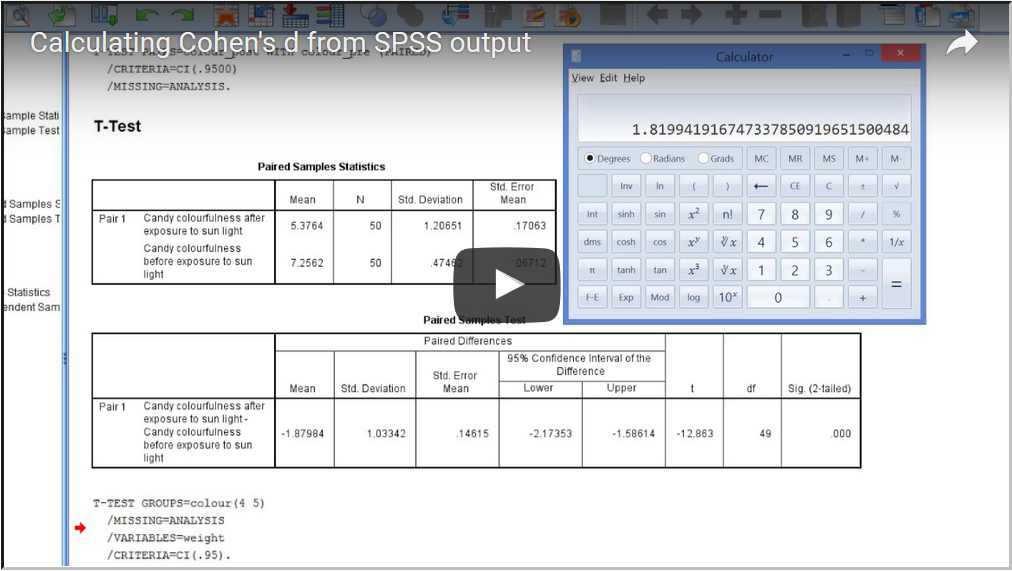
\includegraphics[width=320px]{GentleIntro_files/figure-latex/cohend-1} }\caption{Calculating Cohen's d from SPSS output.}\label{fig:cohend}
\end{figure}

\subsubsection{Exercises}\label{exercises-4}

\begin{enumerate}
\def\labelenumi{\arabic{enumi}.}
\tightlist
\item
  Open data set
  \href{http://82.196.4.233:3838/data/voters.sav}{voters.sav} that
  contains information about the age and attitude towards immigration
  among a random sample of voters. What are the unstandardized and
  standardized effect sizes if the hypothesized average attitude towards
  immigrants in the population is 6.0?
\end{enumerate}

\begin{Shaded}
\begin{Highlighting}[]
\OperatorTok{*}\StringTok{ }\NormalTok{Execute a one}\OperatorTok{-}\NormalTok{sample t test with }\FloatTok{6.0}\NormalTok{ as test value.}
\OperatorTok{*}\StringTok{ }\NormalTok{The reported mean difference }\KeywordTok{is}\NormalTok{ (}\OperatorTok{-}\NormalTok{)}\FloatTok{0.5}\NormalTok{; this is the unstandardized effect}
\NormalTok{size.}
\OperatorTok{*}\StringTok{ }\NormalTok{To obtain the standardized effect }\KeywordTok{size}\NormalTok{ (Cohen}\StringTok{'s d in this case), divide the}
\StringTok{unstandardized effect size by the standard deviation of the variable (here:}
\StringTok{attitude towards immigration), which is reported to be 1.939 Cohen'}\NormalTok{s }\DataTypeTok{d =} \FloatTok{0.5} \OperatorTok{/}
\FloatTok{1.939}\NormalTok{ =}\StringTok{ }\FloatTok{0.26}\NormalTok{. This is a weak effect.}
\end{Highlighting}
\end{Shaded}

\begin{enumerate}
\def\labelenumi{\arabic{enumi}.}
\setcounter{enumi}{1}
\tightlist
\item
  What are the effect sizes if the null hypothesis states that the
  average attitude towards immigrants in the population is at least 6.0?
  And what if it states that average attitude is at most 6.0?
\end{enumerate}

\begin{Shaded}
\begin{Highlighting}[]
\OperatorTok{*}\StringTok{ }\NormalTok{In a one}\OperatorTok{-}\NormalTok{sided test, we take the boundary }\KeywordTok{value}\NormalTok{ (here}\OperatorTok{:}\StringTok{ }\FloatTok{6.0}\NormalTok{) as the value}
\NormalTok{against which we test. It makes sense to use this value also }\ControlFlowTok{for}\NormalTok{ calculating}
\NormalTok{effect size. The unstandardized and standardized effect sizes, then, are the}
\NormalTok{same as }\ControlFlowTok{in}\NormalTok{ Question }\DecValTok{1}\NormalTok{.}
\OperatorTok{*}\StringTok{ }\NormalTok{One could argue, however, that there is no effect, hence zero effect size,}
\ControlFlowTok{in}\NormalTok{ a right}\OperatorTok{-}\NormalTok{sided test here. If we assume }\ControlFlowTok{for}\NormalTok{ whatever reasons that the}
\NormalTok{population average cannot be below }\FloatTok{6.0}\NormalTok{, a sample average below }\FloatTok{6.0}\NormalTok{ such as }\FloatTok{5.5}
\NormalTok{would have to be due to sampling error. It cannot represent a true effect }\ControlFlowTok{if}
\NormalTok{the population average can only be above }\FloatTok{6.0}\NormalTok{.}
\end{Highlighting}
\end{Shaded}

\begin{enumerate}
\def\labelenumi{\arabic{enumi}.}
\setcounter{enumi}{2}
\tightlist
\item
  What are the unstandardized and standardized effect sizes of a test in
  which we compare the attitude towards immigrants of young voters to
  the attitude of old voters? Again, use data set
  \href{http://82.196.4.233:3838/data/voters.sav}{voters.sav}.
\end{enumerate}

\begin{Shaded}
\begin{Highlighting}[]
\OperatorTok{*}\StringTok{ }\NormalTok{Execute an independent}\OperatorTok{-}\NormalTok{samples t test with groups defined by the variable}
\NormalTok{age_group.}
\OperatorTok{*}\StringTok{ }\NormalTok{The reported mean difference }\KeywordTok{is}\NormalTok{ (}\OperatorTok{-}\NormalTok{)}\FloatTok{0.718}\NormalTok{; this is the unstandardized effect}
\NormalTok{size.}
\OperatorTok{*}\StringTok{ }\NormalTok{We approximate the standardized effect }\KeywordTok{size}\NormalTok{ (Cohen}\StringTok{'s d in this case) by}
\StringTok{dividing twice the t value by the square root of the degrees of freedom. Note}
\StringTok{that the F test on equality of population variances is statistically}
\StringTok{significant (p = .029), so we do not assume equal variances and we use the}
\StringTok{bottom row from the results table.}
\StringTok{* Cohen'}\NormalTok{s }\DataTypeTok{d =} \DecValTok{2} \OperatorTok{*}\StringTok{ }\FloatTok{1.602} \OperatorTok{/}\StringTok{ }\KeywordTok{sqrt}\NormalTok{(}\FloatTok{30.009}\NormalTok{) =}\StringTok{ }\FloatTok{3.204} \OperatorTok{/}\StringTok{ }\FloatTok{5.478}\NormalTok{ =}\StringTok{ }\FloatTok{0.58}\NormalTok{. This is a}
\NormalTok{moderate effect.}
\OperatorTok{*}\StringTok{ }\NormalTok{Note that the sample of young voters is too small to conduct a t test. This,}
\NormalTok{however, is not consequential to Cohen}\StringTok{'s d because a minimum sample size is}
\StringTok{required for a reliable p value but not for a t value.}
\end{Highlighting}
\end{Shaded}

\subsection{Association as effect size}\label{assoc-size}

Measures of association such as Pearson's product-moment correlation
coefficient or Spearman's rank correlation coefficient express effect
size if the null hypothesis expects no correlation in the population. If
zero correlation is expected, a correlation coefficient calculated for
the sample expresses the difference between what is observed (sample
correlation) and what is expected (zero correlation in the population).

Effect size is also zero according to the standard null hypotheses used
for tests on the regression coefficient (\emph{b}),
\emph{R}\textsuperscript{2} for the regression model, and
eta\textsuperscript{2} for analysis of variance. As a result, we can use
the standardized regression coefficient (Beta in SPSS and \emph{b}*
according to APA6), \emph{R}\textsuperscript{2}, and
eta\textsuperscript{2} as standardized effect sizes.

Because they are standardized, we can interpret their effect sizes using
rules of thumb, e.g., an association between 0 and .10 is interpreted as
no or a very weak association, between .10 and .30 is weak, between .30
and .50 is moderate, .50 to .80 is strong, and .80 to 1.00 is very
strong, while exactly 1.00 is a perfect association (if 1.00 is the
maximum value). Note that we ignore the sign (plus or minus) of the
effect if we interpret its size.

\subsection{Standardized effect size and sample
size}\label{standardized-effect-size-and-sample-size}

We can use standardized effect size to express the effects that we are
interested in without caring about the precise size of differences. We
merely have to choose whether small, moderate, or large effects are of
practical interest to us. Preferably, we know from previous research
whether small, moderate, or large effects are common in our type of
research. If moderate or large effects are rare, we should use a sample
size that allows detecting small effects. In contrast, when large
effects occur frequently, we can do with a smaller sample that may
overlook small effects.

If we know the effect size in the sample for which we want statistically
significant results, we can figure out the minimum sample size for which
the test statistic is statistically significant.

\begin{figure}[H]
\href{http://82.196.4.233:3838/apps/sample-size/}{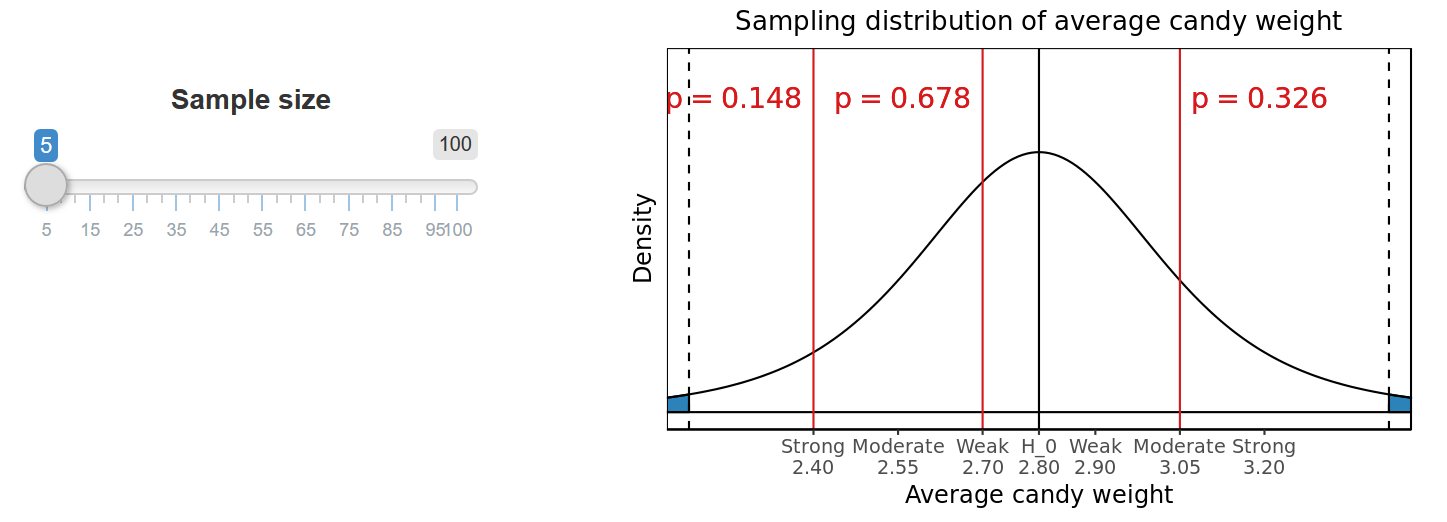
\includegraphics[width=420px]{GentleIntro_files/figure-latex/sample-size-1} }\caption{What is the minimum sample size required for a significant two-sided test result if the sample mean has a particular effect size?}\label{fig:sample-size}
\end{figure}

\begin{enumerate}
\def\labelenumi{\arabic{enumi}.}
\tightlist
\item
  Use the slider in Figure \ref{fig:sample-size} to find the minimum
  sample size that we need for a statistically significant test result
  for each of the three effect sizes represented by red lines.
\end{enumerate}

\begin{Shaded}
\begin{Highlighting}[]
\OperatorTok{*}\StringTok{ }\NormalTok{We need a sample of minimum size }\DecValTok{9}\NormalTok{ to have a statistically significant result}
\ControlFlowTok{for}\NormalTok{ a sample with average weight }\FloatTok{2.40}\NormalTok{ grams, which represents a strong effect.}
\NormalTok{With }\DecValTok{9}\NormalTok{ observations }\ControlFlowTok{in}\NormalTok{ the sample, the red line of a strong effect is }\ControlFlowTok{in}\NormalTok{ the}
\FloatTok{2.5}\NormalTok{% tail of the sampling distribution. The p value is below .}\DecValTok{05}\NormalTok{.}
\OperatorTok{*}\StringTok{ }\NormalTok{For a moderate effect, we need a sample of at least }\DecValTok{18}\NormalTok{ observations.}
\OperatorTok{*}\StringTok{ }\NormalTok{For a weak effect, we need no less than }\DecValTok{99}\NormalTok{ observations.}
\OperatorTok{*}\StringTok{ }\NormalTok{By the way, some of these  sample sizes are too small }\ControlFlowTok{for}\NormalTok{ using the t}
\NormalTok{distribution as approximation of the sampling distribution. Here, the rule of}
\KeywordTok{thumb}\NormalTok{ (}\DecValTok{31}\NormalTok{ cases) has precedence.}
\end{Highlighting}
\end{Shaded}

\begin{enumerate}
\def\labelenumi{\arabic{enumi}.}
\setcounter{enumi}{1}
\tightlist
\item
  What is the meaning of the p values and why do they decrease if we
  increase sample size?
\end{enumerate}

\begin{Shaded}
\begin{Highlighting}[]
\OperatorTok{*}\StringTok{ }\NormalTok{The p values give }\KeywordTok{the}\NormalTok{ (two}\OperatorTok{-}\NormalTok{sided) probability to draw a sample with average}
\NormalTok{candy weight at least as different from the hypothesized value as the value on}
\NormalTok{the horizontal axis.}
\OperatorTok{*}\StringTok{ }\NormalTok{For example, the leftmost red line represents a strong effect }\ControlFlowTok{for}\NormalTok{ a sample}
\NormalTok{with average weight }\FloatTok{2.40}\NormalTok{ grams under the null hypothesis that average candy}
\NormalTok{weight is }\FloatTok{2.80} \ControlFlowTok{in}\NormalTok{ the population. The associated p value informs us that we}
\NormalTok{have }\FloatTok{14.8}\NormalTok{% probability of drawing a sample with average weight at least }\FloatTok{0.40}
\NormalTok{(}\FloatTok{2.80} \OperatorTok{-}\StringTok{ }\FloatTok{2.40}\NormalTok{) grams different from the hypothesized }\KeywordTok{value}\NormalTok{ (}\FloatTok{2.80}\NormalTok{). Differences}
\NormalTok{of at least }\FloatTok{0.40}\NormalTok{ represent strong effects }\ControlFlowTok{in}\NormalTok{ this example, so the p value}
\NormalTok{tells us the probability of finding a strong effect }\ControlFlowTok{in}\NormalTok{ our sample }\ControlFlowTok{if}\NormalTok{ the null}
\NormalTok{hypothesis is true.}
\OperatorTok{*}\StringTok{ }\NormalTok{The larger the sample, the smaller the standard error, the narrower the}
\NormalTok{sampling distribution, the smaller the probability of drawing a sample with an}
\NormalTok{average candy weight that differs from the hypothesized value purely by}
\NormalTok{chance.}
\end{Highlighting}
\end{Shaded}

\begin{enumerate}
\def\labelenumi{\arabic{enumi}.}
\setcounter{enumi}{2}
\tightlist
\item
  Compare the p values to the blue tails. Is there something wrong in
  this app?
\end{enumerate}

\begin{Shaded}
\begin{Highlighting}[]
\OperatorTok{*}\StringTok{ }\NormalTok{There is nothing wrong }\ControlFlowTok{in}\NormalTok{ this app. The p values are two}\OperatorTok{-}\NormalTok{sided but each tail}
\NormalTok{represents only half of the significance level. As a consequence, the p value}
\NormalTok{is twice the surface of the tail to its right or to its left.}
\end{Highlighting}
\end{Shaded}

Effect size as well as test statistics reflect the difference between
what we expect according to the null hypothesis and what we observe in
our sample. As a consequence, effect size indicators and test statistics
are related. In some cases, such as Cohen's d, the relation between
effect size and test statistic is very simple.

The test statistic t for a t test on one mean, for example, is equal to
Cohen's d times the square root of sample size. Here, the only
difference between the two is sample size! Sample size influences the
test statistic---the larger the sample, the larger the test statistic.
At the same time, effect size affects the test statistic---a larger
effect size produces a larger test statistic.

\section{Hypothetical World Versus Imaginary True
World}\label{hypothetical-world-versus-imaginary-true-world}

In the preceding paragraphs, we determined sample size using the effect
size that we expect to find in our sample. We should realize, however,
that we are interested in the effect size in the population. The `true'
effect size, so to speak.

The effect of a new medicine or media campaign in our sample is not
important but the effect in the population is. This complicates the
calculation of sample size. Instead of using the effect size in our
(future!) sample, we must use the effect size in the population.

\subsection{Imagining a population with a small
effect}\label{imagining-a-population-with-a-small-effect}

Our null hypothesis states that average candy weight in the population
is 2.8 grams. Let us decide that a small effect size is practically
significant. We can think now of a population that could be the true
population if the effect size is small. For example, a population in
which average candy weight is 2.9 grams (and the standard deviation is
0.5).

We do not know whether average candy weight is 2.9 grams in the true
population. So we may regard the statement that average candy weight is
2.9 grams in the population as another hypothesis. Let us call this the
alternative hypothesis \emph{H}\textsubscript{1}. Note that this is not
an ordinary alternative hypothesis because it does not include all
outcomes not covered by the null hypothesis (\emph{H}\textsubscript{0}).
Instead, it represents only one value, which is an important value to us
because it represents a population with a small but interesting effect
size.

\begin{center}\rule{0.5\linewidth}{\linethickness}\end{center}

Our habit of formulating a null hypothesis and an alternative hypothesis
for all situations not covered by the null hypothesis is generally
attributed to the statistician R.A. Fisher. This, however, is not
entirely correct (see, e.g., Halpin \& Stam,
\protect\hyperlink{ref-RefWorks:3931}{2006}). Fisher introduced the
concept of a null hypothesis (Ronald Aylmer Fisher,
\protect\hyperlink{ref-RefWorks:3932}{1935}: 18) but not the concept of
an alternative hypothesis. The statisticians Jerzy Neyman and Egon
Pearson introduced the idea of working with two or more hypotheses. But
the two hypotheses do not cover all possible population values and they
were usually not called a null and alternative hypothesis. They specify
two or more different population values. A statistical test is used to
determine which of the hypotheses fits the sample best. (J. Neyman \&
Pearson, \protect\hyperlink{ref-RefWorks:3906}{1933})

\begin{figure}[H]
\centering
\includegraphics{figures/egonpearson.png}
\caption{Egon Pearson}
\end{figure}

\begin{center}\rule{0.5\linewidth}{\linethickness}\end{center}

Figure \ref{fig:TypeI-II-errors} illustrates this situation. The top
graph represents the sampling distribution according to our null
hypothesis. This sampling distribution is derived from our hypothetical
population in which there is no effect, that is, our null hypothesis is
true for this population. In our current example, average candy weight
is 2.8 grams in this hypothetical population.

The bottom graph represents the sampling distribution for an imaginary
population with a small effect size. Here, the alternative hypothesis is
true, for instance, average candy weight is 2.9 grams, which is a bit
higher than in the hypothetical population.

By the way, average population candy weights are not depicted in the
graphs, just the test statistic (t) values. By now, you should know that
the average in a normal or t distribution is situated at the middle
(underneath the top) of the bell shape and that the average of a
sampling distribution for the sample mean is equal to the population
average because a sample mean is an unbiased estimator.

\begin{figure}[H]
\href{http://82.196.4.233:3838/apps/type1vs2/}{\includegraphics[width=430px]{GentleIntro_files/figure-latex/TypeI-II-errors-1} }\caption{Simulation of Type I and Type II error.}\label{fig:TypeI-II-errors}
\end{figure}

Before reading on, try to make sense of the two graphs in Figure
\ref{fig:TypeI-II-errors} and how they relate to each other.

\begin{enumerate}
\def\labelenumi{\arabic{enumi}.}
\tightlist
\item
  What is the relation between significance level and Type I error?
  Formulate your answer very precisely: Details matter now! Check your
  answer by changing the significance level.
\end{enumerate}

\begin{Shaded}
\begin{Highlighting}[]
\OperatorTok{*}\StringTok{ }\NormalTok{With a higher significance }\KeywordTok{level}\NormalTok{ (alpha goes up), we take a larger risk to}
\NormalTok{reject the null hypothesis }\ControlFlowTok{if}\NormalTok{ it is true. The probability of a Type I error,}
\NormalTok{which we make }\ControlFlowTok{if}\NormalTok{ we reject a true null hypothesis, goes up.}
\OperatorTok{*}\StringTok{ }\NormalTok{The orange tails }\ControlFlowTok{in}\NormalTok{ the top graph become bigger and the critical values move}
\NormalTok{towards zero.}
\end{Highlighting}
\end{Shaded}

\begin{enumerate}
\def\labelenumi{\arabic{enumi}.}
\setcounter{enumi}{1}
\tightlist
\item
  What exactly is Type II error?
\end{enumerate}

\begin{Shaded}
\begin{Highlighting}[]
\OperatorTok{*}\StringTok{ }\NormalTok{We make a Type II error }\ControlFlowTok{if}\NormalTok{ we do not reject a false null hypothesis.}
\OperatorTok{*}\StringTok{ }\NormalTok{The situations }\ControlFlowTok{in}\NormalTok{ which we make a Type II error are depicted by the red}
\NormalTok{double}\OperatorTok{-}\NormalTok{sided arrow }\ControlFlowTok{in}\NormalTok{ the bottom graph.}
\end{Highlighting}
\end{Shaded}

\begin{enumerate}
\def\labelenumi{\arabic{enumi}.}
\setcounter{enumi}{2}
\tightlist
\item
  How does the probability of a Type II error relate to the probability
  of a Type I error? Try to explain the relation in your own words.
\end{enumerate}

\begin{Shaded}
\begin{Highlighting}[]
\OperatorTok{*}\StringTok{ }\NormalTok{If the probability of a Type I error goes up, the probability of a Type II}
\NormalTok{error goes down, and the other way around.}
\OperatorTok{*}\StringTok{ }\NormalTok{With a higher significance }\KeywordTok{level}\NormalTok{ (alpha goes up), we take a larger risk to}
\NormalTok{reject the null hypothesis }\ControlFlowTok{if}\NormalTok{ it is true. We have a larger probability of}
\NormalTok{making a Type I error, which is depicted by the orange tails }\ControlFlowTok{in}\NormalTok{ the top graph.}
\OperatorTok{*}\StringTok{ }\NormalTok{If we take a larger risk to reject a true null hypothesis, we reject the}
\NormalTok{null hypothesis more easily.}
\OperatorTok{*}\StringTok{ }\NormalTok{If we reject the null hypothesis more easily, we are more likely to reject}
\NormalTok{the null hypothesis }\ControlFlowTok{if}\NormalTok{ it is not true. The probability to reject a false null}
\NormalTok{hypothesis is the power of the test. This probability is expressed by the}
\NormalTok{orange tail }\ControlFlowTok{in}\NormalTok{ the bottom graph.}
\OperatorTok{*}\StringTok{ }\NormalTok{Note that the critical t values move closer to zero both }\ControlFlowTok{in}\NormalTok{ the top and}
\NormalTok{bottom graph }\ControlFlowTok{if}\NormalTok{ we take a larger risk to reject a false null hypothesis. The}
\NormalTok{critical t values also demarcate the blue area }\ControlFlowTok{in}\NormalTok{ the bottom graph. Moving}
\NormalTok{towards zero, they decrease the size of the blue area.}
\end{Highlighting}
\end{Shaded}

\subsection{Type I error}\label{type-i-error}

We have two populations, a hypothetical population and an imaginary true
population. Once we have drawn our sample, we only deal with the
hypothetical population, for instance, the top graph in Figure
\ref{fig:TypeI-II-errors}, as we have done in all preceding chapters.

Acting as if the null hypothesis is true, we determine how (un)likely
the sample is that we have drawn. If it is very unlikely, we have a p
value below the significance level and we reject the null hypothesis. We
say: If the null hypothesis is true, our sample is too unlikely, so we
reject the null hypothesis.

We may be wrong. Perhaps the null hypothesis is actually true and we
were just very unfortunate to draw a sample that is very different from
the population. If so, we make a Type I error (see Section
\ref{sig-typeI}). The probability that we will make this error is the
significance level of the test, which is usually set to .05.

\subsection{The world of the
researcher}\label{the-world-of-the-researcher}

This is what we are doing once we have the sample. Let us call this the
world of the researcher. At present, we have not yet stepped into the
world of the researcher because we are still thinking about the size of
the sample that we are going to draw.

We can experiment a bit and that is what we do if we ask ourselves: What
is going to happen to our statistical test if the true population from
which we draw our sample has average candy weight that is a bit higher
(small effect) than candy weight according to our null hypothesis?

\subsection{The alternative world of a small
effect}\label{the-alternative-world-of-a-small-effect}

If we actually sample from this imaginary true population, the bottom
graph in Figure \ref{fig:TypeI-II-errors} represents our true sampling
distribution. It shows us the true probabilities (areas under the curve)
of drawing a sample with a particular minimum or maximum value for the
test statistic t. These are the probabilities of our sample if there is
a small effect in the population.

Now that we know the true sampling distribution if there is a small
effect in the population, we can foresee what is going to happen when we
enter the world of the researcher. The researcher is going to use the
test values of the top graph to decide on the null hypothesis. If the
sample t value is between, say, plus and minus two (the critical values,
t\textsubscript{c} in Figure \ref{fig:TypeI-II-errors}), the researcher
is not going to reject the null hypothesis.

\subsection{Type II error}\label{typeIIerror}

If there is a (small) effect in the population, the null hypothesis is
not true. For example, average candy weight is not 2.8 gram, it is 2.9
gram. If our sample mean is close to 2.8 gram, we may not reject the
null hypothesis even if it is not true. This is a \emph{Type II error}:
not rejecting a false null hypothesis.

The probability that we make a Type II error if there is a small effect
is expressed by the blue section in the bottom graph. It is usually
denoted by the Greek letter beta (\(\beta\)). The blue section
represents the probability of drawing a sample from this population with
a small effect size that has a t value that is NOT in the rejection
region, so the null hypothesis is NOT rejected. See the top graph.

Table \ref{tab:errortable} summarizes the four possible situations that
may arise if we test a null hypothesis. The null hypothesis may be true
or false and we may or may not reject the null hypothesis.

\begin{table}

\caption{\label{tab:errortable}Error types and their probabilities.}
\centering
\fontsize{8}{8}\selectfont
\begin{tabular}[t]{|l|l|l|}
\hline
   & Null is true & Null is false\\
\hline
Null is rejected & Type I error, Significance level (alpha) & No error, Power (1 - beta)\\
\hline
Null is not rejected & No error, (1 - alpha) & Type II error, (beta)\\
\hline
\end{tabular}
\end{table}

\subsection{Power of the test}\label{power-of-the-test}

The probability of NOT making a Type II error is called the \emph{power
of the test}. It is equal to one minus the probability of making a Type
II error, that is, 1 - \(\beta\). The power of the test is represented
by the orange sections in the bottom graph. They represent the
probability of getting a sample t value that makes the researcher reject
the null hypothesis. So a false null hypothesis is rejected and we do
not make an error.

Note that we can reject the null hypothesis in two ways: If our sample
happens to have a test statistic that is much higher than expected under
the null hypothesis or if it is much lower. In the example above, the
imagined true population has a mean that is higher than the hypothesized
population mean. The bulk of the power of the test therefore is in the
right tail of the bottom graph.

However, a little bit of power is situated in the left tail. It is so
small that we usually cannot see the orange section in the left tail of
the bottom graph but the displayed probability shows that it is there.
This is a bit strange because one could say that we reject the null
hypothesis for the wrong reason: We think our null hypothesis is too
high whereas it actually is too low.

The probability that this happens is very small and usually negligible.
In the interactive content, you may encounter power values in the left
tail that are so small that they have to be written in scientific
notation, e.g., 1.0E-10, which means 1 at the tenth decimal place:
0.0000000001. Anyway, the important thing is that we reject a false null
hypothesis even if it is for the `wrong' reason. The decision to reject
the null hypothesis is right because the null hypothesis is false.
Unfortunately, in this situation our conclusion that the population
value is below the hypothesized value would be wrong.

\section{Sample Size, Effect Size, and
Power}\label{sample-size-effect-size-and-power}

Finally, after all these sections, we can answer the question raised in
the beginning of this chapter: How large should my sample be? To answer
this question, we must consider the significance level, effect size, and
test power.

\begin{figure}[H]
\href{http://82.196.4.233:3838/apps/sample-size-power/}{\includegraphics[width=320px]{GentleIntro_files/figure-latex/sample-size-power-1} }\caption{How does sample size depend on test power, significance, and effect size?}\label{fig:sample-size-power}
\end{figure}

\begin{enumerate}
\def\labelenumi{\arabic{enumi}.}
\tightlist
\item
  Figure \ref{fig:sample-size-power} shows the sampling distributions of
  the sample mean under the null hypothesis (H\textsubscript{0},
  left-hand curve) and under the assumed true value of the population
  mean (H\textsubscript{1}, right-hand curve). Explain the meaning of
  the red, yellow, and blue surfaces in the graph.
\end{enumerate}

\begin{Shaded}
\begin{Highlighting}[]
\OperatorTok{*}\StringTok{ }\NormalTok{The red areas represent the significance level of the null hypothesis test,}
\NormalTok{namely the total probability of rejecting the null hypothesis }\ControlFlowTok{if}\NormalTok{ it is true.}
\OperatorTok{*}\StringTok{ }\NormalTok{The yellow area gives the probability that we draw a sample from a population}
\NormalTok{with true mean H1 which does not reject the null hypothesis. With these}
\NormalTok{samples, we do not reject the null hypothesis, which is false, so we make a}
\NormalTok{Type II error. The yellow area is the probability of making a Type II error.}
\OperatorTok{*}\StringTok{ }\NormalTok{The blue }\KeywordTok{area}\NormalTok{ (including the red tail at the right) is the probability that}
\NormalTok{we draw a sample from a population with true mean H1 that rejects the null}
\NormalTok{hypothesis, which is false so we do not make a Type II error. It is the}
\NormalTok{probability that we reject a false null hypothesis, which is the power of the}
\NormalTok{test.}
\end{Highlighting}
\end{Shaded}

\begin{enumerate}
\def\labelenumi{\arabic{enumi}.}
\setcounter{enumi}{1}
\tightlist
\item
  What happens to the red, yellow, and blue surfaces if you set power to
  50\%? And what happens to the minimum sample size? Adjust the power
  slider to check your answers.
\end{enumerate}

\begin{Shaded}
\begin{Highlighting}[]
\OperatorTok{*}\StringTok{ }\NormalTok{If we set power to }\DecValTok{50}\NormalTok{%, the yellow and blue areas each should occupy half of}
\NormalTok{the sampling distribution that is centred at H1.}
\OperatorTok{*}\StringTok{ }\NormalTok{A smaller power implies that we run a larger risk of not rejecting a false}
\NormalTok{null hypothesis, so we can do with a smaller sample.}
\end{Highlighting}
\end{Shaded}

\begin{enumerate}
\def\labelenumi{\arabic{enumi}.}
\setcounter{enumi}{2}
\tightlist
\item
  Do we need a smaller or a larger sample to achieve the specified test
  power for a larger effect size? Move the effect size slider to check
  your answer.
\end{enumerate}

\begin{Shaded}
\begin{Highlighting}[]
\OperatorTok{*}\StringTok{ }\NormalTok{With larger effect size, the difference between the true population mean}
\NormalTok{(H1) and the population mean according to the null }\KeywordTok{hypothesis}\NormalTok{ (H0) is}
\NormalTok{larger, and it will be more easily spotted }\ControlFlowTok{in}\NormalTok{ a smaller sample. In other words,}
\NormalTok{we have higher power with a larger effect size. We can do with a smaller sample to}
\NormalTok{achieve the original test power.}
\end{Highlighting}
\end{Shaded}

\begin{enumerate}
\def\labelenumi{\arabic{enumi}.}
\setcounter{enumi}{3}
\tightlist
\item
  Do we need a smaller or a larger sample to achieve the specified test
  power for a one-sided test instead of a two-sided test? Change the
  test type to check your answer.
\end{enumerate}

\begin{Shaded}
\begin{Highlighting}[]
\OperatorTok{*}\StringTok{ }\NormalTok{With a one}\OperatorTok{-}\NormalTok{sided test, the total significance }\KeywordTok{level}\NormalTok{ (red area) is situated }\ControlFlowTok{in}
\NormalTok{one tail. If this tail is at the right side, namely, at the side of the true}
\NormalTok{population mean, we are more likely to reject the null hypothesis with a sample}
\NormalTok{from the true }\KeywordTok{population}\NormalTok{ (the blue area becomes larger), so test power}
\NormalTok{increases }\ControlFlowTok{if}\NormalTok{ we keep the same sample size. To maintain the original test power,}
\NormalTok{we may draw a smaller sample.}
\end{Highlighting}
\end{Shaded}

\begin{enumerate}
\def\labelenumi{\arabic{enumi}.}
\setcounter{enumi}{4}
\tightlist
\item
  Do we need a smaller or a larger sample to achieve the specified test
  power for a higher significance level, for example, \(\alpha = 0.10\)?
  Move the significance level slider to check your answer.
\end{enumerate}

\begin{Shaded}
\begin{Highlighting}[]
\OperatorTok{*}\StringTok{ }\NormalTok{A higher significance level, }\ControlFlowTok{for}\NormalTok{ instance, }\DecValTok{10}\OperatorTok\NormalTok{, has the same effect}
\NormalTok{as a change from a two}\OperatorTok{-}\NormalTok{sided test to a one}\OperatorTok{-}\NormalTok{sided test. We are more likely to}
\NormalTok{reject the null hypothesis, so we are more likely to reject a false null}
\NormalTok{hypothesis, so we have higher test power. To maintain the original test power,}
\NormalTok{we may draw a smaller sample.}
\end{Highlighting}
\end{Shaded}

\begin{enumerate}
\def\labelenumi{\arabic{enumi}.}
\setcounter{enumi}{5}
\tightlist
\item
  Why do the sampling distributions become wider if we increase effect
  size or significance level, or if we decrease test power?
\end{enumerate}

\begin{Shaded}
\begin{Highlighting}[]
\OperatorTok{*}\StringTok{ }\NormalTok{With larger effect size or significance level and with smaller test power,}
\KeywordTok{the}\NormalTok{ (required) sample size decreases. Lower sample sizes produce larger}
\NormalTok{standard errors, which produce a wider distribution because sample results are}
\NormalTok{on average further away from the mean of the distribution.}
\end{Highlighting}
\end{Shaded}

Sample size, statistical significance, effect size, and test power are
related. To determine the size of your sample, you have three sliders
that you should adjust simultaneously. Statistical significance is the
easiest slider to decide on; we usually leave the significance level at
.05. We do not select a smaller value because it will reduce the power
of the test (with the same sample and effect size) as you may have
noticed in one of the figures in the preceding section.

For effect size, we have to choose among a small, moderate, or large
effect. Previous results of research similar to our research project can
help us decide whether we have to reckon with small effect sizes (need a
larger sample) or not. If we have a concrete number for the
(standardized) minimum effect size that is of practical significance, we
can use that number.

For power, the conventional rule of thumb is that we like to have at
least 80\% probability of rejecting a false null hypothesis. You may
note that the probability of NOT rejecting a true null hypothesis is
higher: .95. After all, it is one minus the probability of rejecting a
true null hypothesis (Type I error), which is the significance level.

Power is set to a lower level because the null hypothesis is usually
assumed to reflect our best knowledge about the world. From this
perspective, we are keener on avoiding the error of falsely rejecting
the null hypothesis (our current best knowledge) than falsely accepting
it. This approach, however, is not without criticisms as we will discuss
in Chapter \ref{crit-discus}. Anyway, if you want to raise the power to
the same level of .95, you can do so; it will require a larger sample.

Unfortunately, test power receives little attention in several software
packages for statistical analysis. Using power and effect size to
calculate the required sample size is usually not provided in the
package. To calculate sample size, we need dedicated software, for
example \href{http://www.gpower.hhu.de/}{GPower}.

\subsection{So how do we determine sample
size?}\label{so-how-do-we-determine-sample-size}

All in all, using effect size and test power to determine the size of
the sample requires several decisions on the part of the researcher. It
can be difficult to specify the effect size that we should expect or
that is practically relevant. If there is little prior research
comparable to our new project, we cannot reasonably specify an effect
size and calculate sample size.

Of course, it is important to ensure that our sample meets the
requirements of the tests that we want to specify (Section
\ref{size-test-req}). In practice, researchers often go well beyond this
minimum. They try to collect as large a sample as is feasible just to be
on the safe side.

Does this mean that all we have learned about effect size and test power
is useless? Certainly not. First of all, we should have learned that
effect size is more important than statistical significance because
effect size relates to practical significance.

Second, test power and Type II errors are important in situations in
which we do not reject the null hypothesis. Then, we should calculate
test power to get an impression of our confidence in the result. Is our
test of sufficient power to yield significant results if there is an
effect in the population? This is the topic of the next section.

\section{Research Hypothesis as Null
Hypothesis}\label{research-hypothesis-as-null-hypothesis}

As noted before (Section \ref{null-alt}), the research hypothesis
usually is the alternative hypothesis. We expect something to change, to
be(come) different rather than be or stay the same. We expect an
association to be present rather than absent.

In this situation, rejection of the null hypothesis supports our
alternative hypothesis, hence our research hypothesis, so we are glad if
we reject the null hypothesis. Of course, we know that we can be wrong.
Our null hypothesis may still be true even if the probability of drawing
a sample like the one we have drawn is so small that we have to reject
the null hypothesis. This is a Type I error.

Fortunately, we know the probability of making this error because it is
the significance level that we have chosen, five per cent usually. We
can live with this probability of making an error if we reject the null
hypothesis. So we are doubly glad: We found support for our research
hypothesis \emph{and} we know how confident we are about this support.

What if our research hypothesis is our null hypothesis? For example, we
have a specific idea of average candy weight in the population from
previous research or from specifications by the candy factory. If we
want to test whether the candies have the hypothesized average weight,
our research hypothesis would specify this average weight. Specifying a
particular value, the research hypothesis must be the null hypothesis
(Section \ref{nullhypothesis}).

If the research hypothesis is the null hypothesis because it contains a
single (two-sided) or boundary (one-sided) value for the population
parameter, we find support for our research hypothesis if we do
\emph{not} reject the null hypothesis. We can be wrong in not rejecting
the null hypothesis. If we do not reject a null hypothesis that is
actually false, we make a Type II error.

The significance level is irrelevant now because the significance level
is the probability of making a Type I error. We do not reject the null
hypothesis, so we can never reject a true null hypothesis (Type I
error). Instead, the probability of making a Type II error is important,
or rather, the probability of not making this error. This is the power
of the test.

So if our research hypothesis represents the null hypothesis and our
research hypothesis is supported (not rejected), we need test power to
know how confident we can be about the support that we have found. Here,
test power is relevant, not statistical significance.

\section{Test Your Understanding}\label{test-your-understanding-4}

\begin{figure}[H]
\href{http://82.196.4.233:3838/apps/type1vs2/}{\includegraphics[width=430px]{GentleIntro_files/figure-latex/test-power-1} }\caption{Effect size, power, Type I and Type II error.}\label{fig:test-power}
\end{figure}

Figure \ref{fig:test-power} shows sampling distributions for two worlds.
Both sampling distributions are approximated with a t distribution. At
the top is the hypothetical world of the researcher. In this
hypothetical world, the researcher's null hypothesis is true, namely
that average candy weight is 2.8 gram in the population. At the bottom
is the real world in which average candy weight is 2.9 gram. The
standard deviation of candy weights is 0.5.

\begin{enumerate}
\def\labelenumi{\arabic{enumi}.}
\tightlist
\item
  What do the values on the horizontal axes mean?
\end{enumerate}

\begin{Shaded}
\begin{Highlighting}[]
\OperatorTok{*}\StringTok{ }\NormalTok{The values on the horizontal axes are t values, that is, the value of the}
\NormalTok{sample statistic, }\ControlFlowTok{for}\NormalTok{ instance, the sample mean, transformed into a t test}
\NormalTok{statistic.}
\end{Highlighting}
\end{Shaded}

\begin{enumerate}
\def\labelenumi{\arabic{enumi}.}
\setcounter{enumi}{1}
\tightlist
\item
  What does t\textsubscript{c} mean?
\end{enumerate}

\begin{Shaded}
\begin{Highlighting}[]
\OperatorTok{*}\StringTok{ }\NormalTok{t}\OperatorTok{~}\NormalTok{c}\OperatorTok{~}\StringTok{ }\NormalTok{is the value of the test statistic t that separates }\KeywordTok{the}\NormalTok{ (usually }\DecValTok{5}\NormalTok{%)}
\NormalTok{most unlikely or most extreme samples from the most likely samples }\ControlFlowTok{if}\NormalTok{ the null}
\NormalTok{hypothesis is true.}
\OperatorTok{*}\StringTok{ }\NormalTok{It is called the critical }\KeywordTok{value}\NormalTok{ (of the test statistic). If the test}
\NormalTok{statistic }\ControlFlowTok{for}\NormalTok{ our sample is beyond this value, we reject the null hypothesis.}
\end{Highlighting}
\end{Shaded}

\begin{enumerate}
\def\labelenumi{\arabic{enumi}.}
\setcounter{enumi}{2}
\tightlist
\item
  Why are the t values and t\textsubscript{c}values exactly the same on
  both horizontal axes?
\end{enumerate}

\begin{Shaded}
\begin{Highlighting}[]
\OperatorTok{*}\StringTok{ }\NormalTok{The researcher only knows the hypothetical world}\OperatorTok{:}\StringTok{ }\NormalTok{What does the sampling}
\NormalTok{distribution look like }\ControlFlowTok{if}\NormalTok{ my null hypothesis is true? She uses the critical}
\NormalTok{values of this hypothetical world.}
\OperatorTok{*}\StringTok{ }\NormalTok{The other graph represents the true sampling distribution. This distribution}
\NormalTok{actually produced the sample that the researcher has drawn. The researcher}
\NormalTok{evaluates the sample drawn from this sampling distribution with the critical}
\NormalTok{values from the hypothetical distribution. Therefore, the t}\OperatorTok{~}\NormalTok{c}\OperatorTok{~}\NormalTok{values from the}
\NormalTok{upper graph are also used }\ControlFlowTok{in}\NormalTok{ the bottom graph.}
\end{Highlighting}
\end{Shaded}

\begin{enumerate}
\def\labelenumi{\arabic{enumi}.}
\setcounter{enumi}{3}
\tightlist
\item
  What is the unstandardized and standardized effect size if average
  candy weight is 2.83 gram in our sample?
\end{enumerate}

\begin{Shaded}
\begin{Highlighting}[]
\OperatorTok{*}\StringTok{ }\NormalTok{The effect size is the difference between the hypothesized population value}
\NormalTok{and the value found }\ControlFlowTok{in}\NormalTok{ the sample. According to the text accompanying the}
\NormalTok{Figure, the hypothesized population mean of candy weight is }\FloatTok{2.8}\NormalTok{ gram.}
\OperatorTok{*}\StringTok{ }\NormalTok{If our sample mean is }\FloatTok{2.83}\NormalTok{ gram, the effect size is the difference, that is,}
\NormalTok{(}\OperatorTok{-}\NormalTok{)}\FloatTok{0.03}\NormalTok{ gram. This is the unstandardized effect size. We usually do not care}
\NormalTok{about the sign of the difference.}
\OperatorTok{*}\StringTok{ }\NormalTok{For the standardized effect size, we divide the unstandardized effect size}
\NormalTok{by the standard deviation of the original variable. The standard deviation of}
\NormalTok{candy }\KeywordTok{weight}\NormalTok{ (}\ControlFlowTok{in}\NormalTok{ the sample) is given as }\FloatTok{0.5}\NormalTok{, so the standardized effect}
\NormalTok{size is }\FloatTok{0.03} \OperatorTok{/}\StringTok{ }\FloatTok{0.5}\NormalTok{ =}\StringTok{ }\FloatTok{0.06}\NormalTok{.}
\OperatorTok{*}\StringTok{ }\NormalTok{Provided that we drop a minus sign }\ControlFlowTok{if}\NormalTok{ it appears, this value is Cohen}\StringTok{'s d.}
\StringTok{* According to the rules of thumb for interpreting Cohen'}\NormalTok{s d, the effect is}
\NormalTok{very weak because it is much less than }\FloatTok{0.20}\NormalTok{.}
\OperatorTok{*}\StringTok{ }\NormalTok{Note that this is the effect size }\ControlFlowTok{in}\NormalTok{ the sample. As an alternative, you can}
\NormalTok{calculate the true effect size as the difference between the hypothesized value}
\NormalTok{and the true value }\ControlFlowTok{in}\NormalTok{ the population. The true unstandardized effect size is}
\FloatTok{2.8} \OperatorTok{-}\StringTok{ }\FloatTok{2.9}\NormalTok{ =}\StringTok{ }\NormalTok{(}\OperatorTok{-}\NormalTok{)}\FloatTok{0.1}\NormalTok{. If we assume that the reported standard deviation of candy}
\KeywordTok{weights}\NormalTok{ (}\FloatTok{0.5}\NormalTok{) applies to the population, the true standardized effect size is}
\NormalTok{(}\FloatTok{2.8} \OperatorTok{-}\StringTok{ }\FloatTok{2.9}\NormalTok{)}\OperatorTok{/}\FloatTok{0.5}\NormalTok{ =}\StringTok{ }\NormalTok{(}\OperatorTok{-}\NormalTok{)}\FloatTok{0.2}\NormalTok{.}
\end{Highlighting}
\end{Shaded}

\begin{enumerate}
\def\labelenumi{\arabic{enumi}.}
\setcounter{enumi}{4}
\tightlist
\item
  What do the double-sided horizontal red arrows represent in the top
  graph?
\end{enumerate}

\begin{Shaded}
\begin{Highlighting}[]
\OperatorTok{*}\StringTok{ }\NormalTok{They represent the values of the t statistic }\ControlFlowTok{for}\NormalTok{ which we reject the null}
\NormalTok{hypothesis. This is called the rejection region of the test.}
\end{Highlighting}
\end{Shaded}

\begin{enumerate}
\def\labelenumi{\arabic{enumi}.}
\setcounter{enumi}{5}
\tightlist
\item
  Why are the double-sided horizontal arrows red in the top graph and
  black in the bottom graph and the other way around?
\end{enumerate}

\begin{Shaded}
\begin{Highlighting}[]
\OperatorTok{*}\StringTok{ }\NormalTok{The red double}\OperatorTok{-}\NormalTok{sided arrows represent errors.}
\OperatorTok{*}\StringTok{ }\NormalTok{In the top graph, they represent the situation that we reject a null}
\NormalTok{hypothesis }\ControlFlowTok{if}\NormalTok{ it is true. This is a Type I error.}
\OperatorTok{*}\StringTok{ }\NormalTok{In the bottom graph, they represent the situation that we do not reject a}
\NormalTok{null hypothesis that is false. This is a Type II error.}
\end{Highlighting}
\end{Shaded}

\begin{enumerate}
\def\labelenumi{\arabic{enumi}.}
\setcounter{enumi}{6}
\tightlist
\item
  Why are the orange sections in the top graph labelled Type I error?
\end{enumerate}

\begin{Shaded}
\begin{Highlighting}[]
\OperatorTok{*}\StringTok{ }\NormalTok{The orange sections represent the probability of rejecting a null hypothesis}
\ControlFlowTok{if}\NormalTok{ it is true. This is a Type I error.}
\OperatorTok{*}\StringTok{ }\NormalTok{Note that a more accurate labelling of the graph would have said}\OperatorTok{:}
\StringTok{"Probability of a Type I error."}
\end{Highlighting}
\end{Shaded}

\begin{enumerate}
\def\labelenumi{\arabic{enumi}.}
\setcounter{enumi}{7}
\tightlist
\item
  What happens to the probability of a Type II error (the blue section
  in the bottom graph) if you change the significance level with the
  slider?
\end{enumerate}

\begin{Shaded}
\begin{Highlighting}[]
\OperatorTok{*}\StringTok{ }\NormalTok{With a higher significance }\KeywordTok{level}\NormalTok{ (alpha goes up), we take a larger risk to}
\NormalTok{reject the null hypothesis }\ControlFlowTok{if}\NormalTok{ it is true. The orange tails }\ControlFlowTok{in}\NormalTok{ the top graph}
\NormalTok{become bigger and the critical values move towards zero.}
\OperatorTok{*}\StringTok{ }\NormalTok{If we take a larger risk to reject a true null hypothesis, we reject the}
\NormalTok{null hypothesis more easily.}
\OperatorTok{*}\StringTok{ }\NormalTok{If we reject the null hypothesis more easily, we are more likely to reject}
\NormalTok{the null hypothesis }\ControlFlowTok{if}\NormalTok{ it is not true. The probability to reject a false null}
\NormalTok{hypothesis is the power of the test. This probability is expressed by the}
\NormalTok{orange tail }\ControlFlowTok{in}\NormalTok{ the bottom graph.}
\OperatorTok{*}\StringTok{ }\NormalTok{If we are more likely to reject a false null hypothesis, we are less likely}
\NormalTok{to make the Type II error of not rejecting a false null hypothesis. This is}
\NormalTok{the blue section }\ControlFlowTok{in}\NormalTok{ the bottom graph.}
\OperatorTok{*}\StringTok{ }\NormalTok{Note that the critical t values move closer to zero both }\ControlFlowTok{in}\NormalTok{ the top and}
\NormalTok{bottom graph }\ControlFlowTok{if}\NormalTok{ we take a larger risk to reject a false null hypothesis. The}
\NormalTok{critical t values also demarcate the blue area }\ControlFlowTok{in}\NormalTok{ the bottom graph. Moving}
\NormalTok{towards zero, they decrease the size of the blue area.}
\end{Highlighting}
\end{Shaded}

\begin{enumerate}
\def\labelenumi{\arabic{enumi}.}
\setcounter{enumi}{8}
\tightlist
\item
  What does \emph{Type II error} mean in the bottom graph?
\end{enumerate}

\begin{Shaded}
\begin{Highlighting}[]
\OperatorTok{*}\StringTok{ }\NormalTok{Type II error is the situation that we do not reject a null hypothesis that}
\NormalTok{is false.}
\end{Highlighting}
\end{Shaded}

\section{Take-Home Points}\label{take-home-points-4}

\begin{itemize}
\item
  Effect size is related to practical significance. Effect sizes are
  expressed by (standardized) mean differences, regression coefficients,
  and measures of association such as the correlation coefficient,
  \emph{R}\textsuperscript{2}, and eta\textsuperscript{2}.
\item
  Statistical significance of a test depends on effect size and sample
  size. Because sample size affects statistical significance, it is
  wrong to use significance or a p value as an indication of effect
  size.
\item
  Not rejecting a false null hypothesis is a Type II error. A researcher
  can make this error only if the null hypothesis is not rejected.
\item
  The probability of making a Type II error is commonly denoted with the
  Greek letter beta (\(\beta\)).
\item
  The probability of \emph{not} making a Type II error is the power of
  the test.
\item
  The power of a test tells us the probability that we reject the null
  hypothesis if there is an effect of a particular size in the
  population. The larger this probability, the more confident we are
  that we do not overlook an effect when we do not reject the null
  hypothesis.
\end{itemize}

\chapter{Critical Discussion of Null Hypothesis Significance
Testing}\label{crit-discus}

\begin{quote}
Key concepts: problems with null hypothesis significance testing,
meta-analysis, replication, frequentist versus Bayesian inference,
theoretical population, data generating process.
\end{quote}

\subsection*{Summary}\label{summary-5}
\addcontentsline{toc}{subsection}{Summary}

\begin{quote}
How important is null hypothesis significance testing?
\end{quote}

In the preceding chapters, we learned to test null hypotheses. Null
hypothesis significance testing is widely used in the social and
behavioral sciences. There are, however, problems with null hypothesis
significance tests that are increasingly being recognized.

The statistical significance of a null hypothesis test depends strongly
on the size of the sample (Chapters \ref{hypothesis} and \ref{power}),
so non-significance may merely mean that the sample is too small. In
contrast, irrelevant tiny effects can be statistically significant in a
very large sample. Finally, we normally test a null hypothesis that
there is no effect whereas we have good reasons to believe that there is
an effect in the population. What does a significant test result really
tell us if we reject an unlikely null hypothesis?

Among the alternatives to null hypothesis significance testing, using a
confidence interval to estimate effects in the population is easiest to
apply. It is closely related to null hypothesis testing, as we have seen
in Section \ref{null-ci0}, but it offers us information with which we
can draw a more nuanced conclusion about our results.

\section{Criticisms of Null Hypothesis Significance
Testing}\label{criticisms-of-null-hypothesis-significance-testing}

In null hypothesis significance testing, we totally rely on the test's p
value. If this value is below .05 or another significance level, we
reject the null hypothesis and we accept it otherwise. Is this a wise
thing to do? Watch the video.

\href{https://www.youtube.com/embed/ez4DgdurRPg}{\includegraphics{GentleIntro_files/figure-latex/pdance-1.png}}

\subsection{Statistical significance is not a measure of effect
size}\label{statistical-significance-is-not-a-measure-of-effect-size}

Perhaps, Chapter \ref{hypothesis} on null hypothesis testing should have
been titled \emph{Am I Lucky or Unlucky?} instead of \emph{Am I Right or
Am I Wrong?} When our sample is small, the power to reject a null
hypothesis is rather small, so it often happens that we retain the null
hypothesis even if it is wrong. There is a lot of uncertainty about the
population if our sample is small. So we must be lucky to draw a sample
that is sufficiently at odds with the null hypothesis to reject it.

If our sample is large or very large, small differences between what we
expect according to our null hypothesis can be statistically significant
even if the differences are too small to be of any practical value. A
statistically significant result need not be practically relevant. In
all, statistical significance does not tell us about effect size.

\begin{figure}[H]
\href{http://82.196.4.233:3838/apps/tiny-effects/}{\includegraphics[width=320px]{GentleIntro_files/figure-latex/tiny-effects-1} }\caption{Any effect can be statistically significant.}\label{fig:tiny-effects}
\end{figure}

\begin{enumerate}
\def\labelenumi{\arabic{enumi}.}
\tightlist
\item
  What is the null hypothesis in Figure \ref{fig:tiny-effects} and how
  can you tell?
\end{enumerate}

\begin{Shaded}
\begin{Highlighting}[]
\OperatorTok{*}\StringTok{ }\NormalTok{The null hypothesis states that average candy weight is }\FloatTok{2.8}\NormalTok{ (gram) }\ControlFlowTok{in}\NormalTok{ the}
\NormalTok{population.}
\OperatorTok{*}\StringTok{ }\NormalTok{In a statistical test, the sampling distribution has the hypothesized value}
\NormalTok{as it}\StringTok{'s mean (as its expected value).}
\end{Highlighting}
\end{Shaded}

\begin{enumerate}
\def\labelenumi{\arabic{enumi}.}
\setcounter{enumi}{1}
\tightlist
\item
  In Figure \ref{fig:tiny-effects}, what should you do to obtain a
  statistically significant result for a sample average of 2.9 gram if
  the null hypothesis states that average candy weight is 2.8?
\end{enumerate}

\begin{Shaded}
\begin{Highlighting}[]
\OperatorTok{*}\StringTok{ }\NormalTok{Increase sample size. Already at a sample size of }\DecValTok{140}\NormalTok{, a sample with average}
\NormalTok{candy weight of }\FloatTok{2.9}\NormalTok{ gram differs significantly from the hypothesized }\FloatTok{2.8}\NormalTok{ gram.}
\NormalTok{In other words, a sample of this size with an average }\KeywordTok{of}\NormalTok{ (at least) }\FloatTok{2.9}\NormalTok{ is quite unlikely}
\NormalTok{to be drawn from the hypothesized population with an average of }\FloatTok{2.8}\NormalTok{.}
\end{Highlighting}
\end{Shaded}

\begin{enumerate}
\def\labelenumi{\arabic{enumi}.}
\setcounter{enumi}{2}
\tightlist
\item
  Can you get a statistically significant result for the smallest effect
  size, that is, for the smallest non-zero difference between the
  observed sample average and the hypothesized population average?
\end{enumerate}

\begin{Shaded}
\begin{Highlighting}[]
\OperatorTok{*}\StringTok{ }\NormalTok{The smallest sample mean larger than }\FloatTok{2.8}\NormalTok{ that we can select with the sample}
\NormalTok{average slider is }\FloatTok{2.81}\NormalTok{. The smallest non}\OperatorTok{-}\NormalTok{zero difference between sample mean}
\NormalTok{and hypothesized population average, then, is .}\DecValTok{01}\NormalTok{ (gram).}
\OperatorTok{*}\StringTok{ }\NormalTok{A sample of about }\DecValTok{14}\NormalTok{,}\DecValTok{000}\NormalTok{ observations will give a statistically significant}
\NormalTok{test result.}
\OperatorTok{*}\StringTok{ }\NormalTok{So yes, we can get a statistically significant result }\ControlFlowTok{for}\NormalTok{ the smallest}
\NormalTok{non}\OperatorTok{-}\NormalTok{zero effect size.}
\OperatorTok{*}\StringTok{ }\NormalTok{A difference of }\FloatTok{0.01} \KeywordTok{gram}\NormalTok{ (less than }\FloatTok{0.4}\NormalTok{% of the hypothesized weight) may}
\NormalTok{not be practically relevant.}
\end{Highlighting}
\end{Shaded}

\begin{enumerate}
\def\labelenumi{\arabic{enumi}.}
\setcounter{enumi}{3}
\tightlist
\item
  There is one sample mean for which we can never reject the null
  hypothesis, no matter how large we make the sample. Which sample mean
  would that be?
\end{enumerate}

\begin{Shaded}
\begin{Highlighting}[]
\OperatorTok{*}\StringTok{ }\NormalTok{If the sample mean is exactly equal to the hypothesized population mean, }\ControlFlowTok{in}
\NormalTok{this example, exactly }\FloatTok{2.8}\NormalTok{ gram, the null hypothesis will never be rejected.}
\NormalTok{This makes sense because we find exactly what we expect.}
\OperatorTok{*}\StringTok{ }\NormalTok{Increasing sample size reduces the width of the interval between the}
\NormalTok{rejection }\KeywordTok{regions}\NormalTok{ (between the blue tails }\ControlFlowTok{in}\NormalTok{ this graph). But the hypothesized}
\NormalTok{value at the centre of this interval will always fall }\ControlFlowTok{in}\NormalTok{ between the rejection}
\NormalTok{regions.}
\end{Highlighting}
\end{Shaded}

\begin{enumerate}
\def\labelenumi{\arabic{enumi}.}
\setcounter{enumi}{4}
\tightlist
\item
  When is a statistically significant result more surprising: with high
  or low test power? Note: The power calculated in Figure
  \ref{fig:tiny-effects} assumes that average candy weight in the
  population equals average candy weight in the sample.
\end{enumerate}

\begin{Shaded}
\begin{Highlighting}[]
\OperatorTok{*}\StringTok{ }\NormalTok{A statistically significant result is more surprising with low test power.}
\OperatorTok{*}\StringTok{ }\NormalTok{With low test power, the difference between hypothesized and true population}
\NormalTok{values must be quite large to obtain a statistically significant result or we}
\NormalTok{must be very lucky. In this sense, a statistically significant result is more}
\NormalTok{surprising with low test power than with high test power.}
\OperatorTok{*}\StringTok{ }\NormalTok{With low test power, we are more likely to have an effect that is}
\NormalTok{practically relevant.}
\end{Highlighting}
\end{Shaded}

It is a common mistake to think that statistical significance is a
measure of the strength or practical significance of an effect. In the
video (Figure \ref{fig:pdance}), this mistaken interpretation is
expressed by the type of sound associated with a p value: the lower the
p value of the test, the more joyous the sound.

It is wrong to use statistical significance as a measure of strength or
importance. In a large sample, even irrelevant results can be highly
significant and in small samples, as demonstrated in the video, results
can sometimes be highly significant and sometimes be insignificant.
Never forget:

\begin{quote}
A statistically significant result ONLY means that the null hypothesis
must be rejected.
\end{quote}

If we want to say something about the magnitude of an effect in the
population, we should use effect size. All we have is the effect size
measured in our sample and a statistical test usually telling us whether
or not we should reject the null hypothesis that there is no effect in
the population.

If the statistical test is significant, we conclude that an effect
probably exists in the population. We may use the effect size in the
sample as a point estimate of the population effect. This effect size
should be at the core of our interpretation. Is it large (strong), small
(weak), or perhaps tiny and practically irrelevant?

If the statistical test is not significant, it is tempting to conclude
that the null hypothesis is true, namely, that there is no effect in the
population and we need not interpret the effect that we find in our
sample. But this is not right. Finding insufficient proof for rejecting
the null hypothesis does not prove that the null hypothesis is true.

In a two-sided significance test, the null hypothesis specifies one
particular value for the sample outcome. If the outcome is continuous,
for instance, a mean or regression coefficient, the null hypothesis can
hardly ever be true. The true population value is very likely not
exactly the same as the hypothesized value. It may be only slightly
different, but it is different.

Instead of focusing on true versus false, we had better take into
account the probability that we reject the null hypothesis, which is
test power. If test power is low, as it often is in social scientific
research without very large samples, we should realize that there can be
a substantive difference between true and hypothesized population values
even if the test is not statistically significant.

With low power, we have high probability of not rejecting a false null
hypothesis even if the true population value is quite different from the
hypothesized value. For example, a small sample of candies drawn from a
population with average candy weight of 3.0 gram may not reject the null
hypothesis that average candy weight is 2.8 gram in the population. The
statistical test result should not make us conclude that there is no
interesting effect. The test may not pick up substantively interesting
effects.

In contrast, if our test has very high power, we should expect effects
to be statistically significant. Even tiny effects that are totally
irrelevant from a substantive point of view. For example, an effect of
exposure on attitude of 0.01 on 10-point scales, is likely to be
statistically significant in a very large sample but it is substantively
uninteresting.

As noted before (Section \ref{typeIIerror}), standard statistical
software usually does not report the power of a test. For this reason,
it is not common practice to evaluate the statistical significance of
results in combination with test power.

By now, however, you understand that test power is affected by sample
size. You should realize that null hypotheses are easily rejected in
large samples but they are more difficult to reject in small samples.
Don't let your selection of interesting results be guided predominantly
by statistical significance if your sample is not very large.

\subsection{Knocking down straw men (over and over
again)}\label{strawmen}

There is another aspect in the practice of null hypothesis significance
testing that is not very satisfactory. Remember that null hypothesis
testing was presented as a means for the researcher to use previous
knowledge as input to her research (Section \ref{binarydecision}). The
development of science requires us to expand existing knowledge. Does
this really happen in the practice of null hypothesis significance
testing?

Imagine that previous research has taught us that one additional unit of
exposure to advertisements for a brand increases a person's brand
awareness on average by 0.1 unit if we use well-tested standard scales
for exposure and brand awareness. If we want to use this knowledge in
our own research, we would hypothesize that the regression coefficient
of exposure is 0.1 in a regression model predicting brand awareness.

Well, try to test this null hypothesis in your favourite statistics
software. Can you actually tell the software that the null hypothesis
for the regression coefficient is 0.1? Most likely you can't because the
software automatically tests the null hypothesis that the regression
coefficient is zero in the population.

This approach is so prevalent that null hypotheses equating the
population value of interest to zero have received a special name: the
\emph{nil hypothesis} or \emph{the nil} for short (see Section
\ref{null-alt}). How can we include previous knowledge in our test if
the software always tests the nil?

The null hypothesis that there is no association between the independent
variable and the dependent variable in the population may be interesting
to reject if you really have no clue about the association. But in the
example above, previous knowledge makes us expect a positive association
of a particular size. Here, it is not interesting to reject the null
hypothesis of no association. The null hypothesis of no association is a
\emph{straw man} in this example. It is unlikely to stand the test and
nobody should applaud if we knock it down.

Rejecting the nil time and again should make us wonder about scientific
progress and our contribution to it. Are we knocking down straw men
hypotheses over and over again? Is there no way to accumulate our
efforts?

\section{Alternatives for Null Hypothesis Significance
Testing}\label{alternatives-for-null-hypothesis-significance-testing}

In the social and behavioral sciences, null hypothesis testing is still
the dominant type of statistical inference. For this reason, an
introductory text like the current one must discuss null hypothesis
significance testing. But it should discuss it thoroughly, so the
problems and errors that occur with null hypothesis testing become clear
and can be avoided.

The problems with null hypothesis significance testing are increasingly
being recognized. Alternatives to null hypothesis significance testing
have been developed and are becoming more accepted within the field. In
this section, some alternatives are briefly sketched.

\subsection{Estimation instead of hypothesis
testing}\label{estimation-instead-of-hypothesis-testing}

Following up on a report commissioned by the American Psychological
Association APA (Wilkinson,
\protect\hyperlink{ref-RefWorks:3934}{1999}), the 6\textsuperscript{th}
edition of the \emph{Publication Manual of the American Psychological
Association} recommends reporting and interpreting confidence intervals
rather than relying solely on null hypothesis tests.

Estimation is becoming more important: Assessing the precision of our
statements about the population rather than deciding pro or con our
hypothesis about the population. This is an important step forward and
it is easy to accomplish if your statistical software reports confidence
intervals.

\begin{figure}[H]
\centering
\includegraphics{GentleIntro_files/figure-latex/ci-nullhyp-1.pdf}
\caption{\label{fig:ci-nullhyp}What is the most sensible interpretation of
the results represented by the confidence interval ?}
\end{figure}

Figure \ref{fig:ci-nullhyp} shows six confidence intervals for a
population value, for instance, the effect of exposure to advertisements
on brand awareness, and the sample result as point estimate (dot). The
horizontal axis is labeled by the size of the effect: the difference
between the effect in the sample and the absence of an effect according
to the null hypothesis.

\begin{enumerate}
\def\labelenumi{\arabic{enumi}.}
\tightlist
\item
  Would you advise the company to use the advertisement based on a null
  hypothesis significance test?
\end{enumerate}

\begin{Shaded}
\begin{Highlighting}[]
\OperatorTok{*}\StringTok{ }\NormalTok{If the }\DecValTok{95}\NormalTok{% confidence interval does not include }\KeywordTok{H0}\NormalTok{ (the vertical line), we}
\NormalTok{must reject the null hypothesis at the }\DecValTok{5}\NormalTok{% significance level. That is the rule}
\NormalTok{of the game called null hypothesis significance testing.}
\OperatorTok{*}\StringTok{ }\NormalTok{This is the case }\ControlFlowTok{for}\NormalTok{ confidence intervals C, E, and F.}
\OperatorTok{*}\StringTok{ }\NormalTok{If we can reject the null hypothesis, we would be confident that there is an}
\NormalTok{effect of exposure on brand awareness }\ControlFlowTok{in}\NormalTok{ the population. But this can be a}
\NormalTok{tiny }\KeywordTok{effect}\NormalTok{ (interval C), a large }\KeywordTok{effect}\NormalTok{ (interval F), or an effect that is}
\NormalTok{weak to }\KeywordTok{moderate}\NormalTok{ (interval E) }\ControlFlowTok{if}\NormalTok{ we only interpret the effect size }\ControlFlowTok{in}\NormalTok{ the}
\NormalTok{sample as point estimate of the effect }\ControlFlowTok{in}\NormalTok{ the population. In case of a tiny}
\NormalTok{effect, would we recommend to use the advertisement?}
\end{Highlighting}
\end{Shaded}

\begin{enumerate}
\def\labelenumi{\arabic{enumi}.}
\setcounter{enumi}{1}
\tightlist
\item
  Would you advise the company to use the advertisement based on the
  confidence intervals in Figure \ref{fig:ci-nullhyp}?
\end{enumerate}

\begin{Shaded}
\begin{Highlighting}[]
\OperatorTok{*}\StringTok{ }\NormalTok{If less of the confidence interval extends to the left of }\KeywordTok{H0}\NormalTok{ (negative effect)}
\NormalTok{and more of it is situated to the }\KeywordTok{right}\NormalTok{ (positive effect), we are more}
\NormalTok{confident that the effect is positive }\ControlFlowTok{in}\NormalTok{ the population. If the range of}
\NormalTok{plausible population values is more strongly positive, we are more certain}
\NormalTok{that there is a substantial positive effect }\ControlFlowTok{in}\NormalTok{ the population. This is the}
\NormalTok{most important reason }\ControlFlowTok{for}\NormalTok{ using the advertisement.}
\OperatorTok{*}\StringTok{ }\NormalTok{Interval F offers the most convincing evidence }\ControlFlowTok{for}\NormalTok{ a substantial positive}
\NormalTok{effect. Intervals D and E also suggest a positive effect but we are not so}
\NormalTok{sure about the size of the effect}\OperatorTok{:}\StringTok{ }\NormalTok{it may be tiny or perhaps even absent but}
\NormalTok{it can also be moderate to strong.}
\end{Highlighting}
\end{Shaded}

A confidence interval shows us whether or not our null hypothesis must
be rejected (see Section \ref{null-ci0}). The rule is simple: If the
value of the null hypothesis is within the confidence interval, the null
hypothesis must not be rejected. By the way, note that a confidence
interval allows us to test a null hypothesis other than the nil (Section
\ref{strawmen}). If we hypothesize that the effect of exposure on brand
awareness is 0.1, we reject the hypothesis if the confidence interval of
the regression coefficient does not include 0.1.

At the same time, however, confidence intervals allow us to draw a more
nuanced conclusion. A confidence interval displays our uncertainty about
the result. If the confidence interval is wide, we are quite uncertain
about the true population value. If a wide confidence interval includes
the null hypothesis near one of its boundaries, we do not reject the
null hypothesis but it still is plausible that the population value is
substantially larger (or substantially smaller) than the hypothesized
value.

We should report that the population value seems to be larger (smaller)
than specified in the null hypothesis but that we have inconclusive
evidence because the test is not statistically significant. This is
better than reporting that there is no difference because the
statistical test is not significant.

\begin{center}\rule{0.5\linewidth}{\linethickness}\end{center}

The fashion of speaking of a null hypothesis as ``accepted when false'',
whenever a test of significance gives us no strong reason for rejecting
it, and when in fact it is in some way imperfect, shows real ignorance
of the research workers' attitude, by suggesting that in such a case he
has come to an irreversible decision.

The worker's real attitude in such a case might be, according to the
circumstances:

\begin{enumerate}
\def\labelenumi{(\alph{enumi})}
\tightlist
\item
  ``The possible deviation from truth of my working hypothesis, to
  examine which the test is appropriate, seems not to be of sufficient
  magnitude to warrant any immediate modification.''
\end{enumerate}

Or it might be:

\begin{enumerate}
\def\labelenumi{(\alph{enumi})}
\setcounter{enumi}{1}
\tightlist
\item
  ``The deviation is in the direction expected for certain influences
  which seemed to me not improbable, and to this extent my suspicion has
  been confirmed; but the body of data available so far is not by itself
  sufficient to demonstrate their reality.''
\end{enumerate}

(Ronald Aylmer Fisher, \protect\hyperlink{ref-RefWorks:3907}{1955}: 73)

\begin{figure}[H]
\centering
\includegraphics{figures/fisher.png}
\caption{Sir Ronald Aylmer Fisher.}
\end{figure}

\begin{center}\rule{0.5\linewidth}{\linethickness}\end{center}

In a similar way, a very narrow confidence interval including the null
hypothesis and a very narrow confidence interval near the null
hypothesis but excluding it should not yield opposite conclusions
because the statistical test is significant in the second but not in the
first situation. After all, even for the significant situation, we know
with high confidence (narrow confidence interval) that the population
value is close to the hypothesized value.

Using confidence intervals in this way, we avoid the problem that
statistically non-significant effects are not published. Not publishing
non-significant results, either because of self-selection by the
researcher or selection by journal editors and reviewers, offers a
misleading view of research results.

If results are not published, they cannot be used to design new research
projects. For example, effect sizes that are not statistically
significant are just as helpful to determine sample size as
statistically significant effect sizes. An independent variable without
statistically significant effect may have a significant effect in a new
research project and should not be discarded if the potential effect
size is so substantial that it is practically significant. Moreover,
combining results from several research projects helps making more
precise estimates of population values, which brings us to
meta-analysis.

\subsection{Meta-analysis}\label{meta-analysis}

Meta-analysis is a method that capitalizes on previous knowledge. In
this method, we collect previous studies on the same topic that use the
same or highly similar variables. Combining the results of these
studies, we can make statements with higher precision about the
population. Basically, we combine the separate samples used for each
single study into a large sample, which reduces the uncertainty and
allows more precise inferences about the population.

Meta-analysis is a good example of combining research efforts to
increase our understanding. It favours estimation over hypothesis
testing because the goal is to obtain more precise estimates of
population values or effects. Meta-analysis is strongly recommended as a
research strategy by Geoff Cumming, who coined the concept \emph{New
Statistics}. See Cumming's book
(\protect\hyperlink{ref-RefWorks:3883}{2012}),
\href{http://www.latrobe.edu.au/psychology/research/research-areas/cognitive-and-developmental-psychology/esci}{website},
or \href{https://www.youtube.com/user/geoffdcumming}{YouTube channel} if
you are curious to learn more. The video at the start of this chapter is
made by Geoff Cumming.

\subsection{Replication}\label{replication}

Another approach that builds upon previous results is
\emph{replication}. If we collect new data on variables that are central
in prior research and we execute the same analyses, we \emph{replicate}
previous research.

Replication is the surest tool to check results of previous research.
Checks do not necessarily serve to expose fraud and mistakes. They tell
us whether prior research results still hold at a later time and perhaps
in another context. Thus, we can decrease the chance that our previous
results derive from an atypical sample. But replication also helps us to
develop more general theories and discard theories that apply only to
special situations.

\subsection{Bayesian inference}\label{bayesian-inference}

A more radical way of including previous knowledge in statistical
inference is \emph{Bayesian inference}. Bayesian inference regards the
sample that we draw as a means to update the knowledge that we already
have or think we have on the population. Our previous knowledge is our
starting point and we are not going to just discard our previous
knowledge if a new sample points in a different direction, as we do when
we reject a null hypothesis.

Think of Bayesian inference as a process similar to predicting the
weather. If I try to predict tomorrow's weather, I am using all my
weather experience to make a prediction. If my prediction turns out to
be more or less correct, I don't change the way I predict the weather.
But if my prediction is patently wrong, I try to reconsider the way I
predict the weather, for example, paying attention to new indicators of
weather change.

Bayesian inference uses a concept of probability that is fundamentally
different from the type of inference presented in previous chapters,
which is usually called \emph{frequentist inference}. Bayesian inference
does not assume that there is a true population value. Instead, it
regards the population value as a random variable, that is, as something
with a probability.

Again, think of predicting the weather. I am not saying to myself: ``Let
us assume that tomorrow will be a rainy day. If this is correct, what is
the probability that the weather today looks like it does?'' Instead, I
think of the probability that it will rain tomorrow. Bayesian
probabilities are much more in line with our everyday concept of
probability than the dice-based probabilities of frequentist inference.

Remember that we are not allowed to interpret the 95\% confidence
interval as the interval within which the parameter lies with 95\%
probability (Chapter \ref{param-estim})? This is because a parameter
does not have a probability in frequentist inference. The \emph{credible
interval} is the Bayesian equivalent of the confidence interval. In
Bayesian inference, a parameter has a probability, so we are allowed to
say that the parameter lies within the credible interval with 95\%
probability. This interpretation is much more in line with our intuitive
notion of probabilities.

Bayesian inference is intuitively appealing but it has not yet spread
widely in the social and behavioral sciences. Therefore, I merely
mention this strand of statistical inference and I refrain from giving
details. Its popularity, however, is increasing, so you may come in
contact with Bayesian inference sooner or later.

\section{What If I Do Not Have a Random Sample?}\label{no-random-sample}

In our approach to statistical inference, we have assumed all the time
that we could have drawn a very large number of random samples from the
same population. The large number of samples constitute the sampling
distribution that tells us about the probability of drawing the one
random sample that we have actually drawn or a sample with a result that
is even further away from the hypothesized value.

What if I do not have a random sample? Can I still estimate confidence
intervals or test null hypotheses? If you carefully read reports of
scientific research, you will encounter examples of statistical
inference on non-random samples or data that are not samples at all but
rather represent an entire population, for instance, all people visiting
a particular web site. Statistical inference is clearly being applied to
data that are not sampled at random from an observable population. The
fact that it happens, however, is not a guarantee that it is right.

We should note that statistical inference based on a random sample is
the most convincing type of inference because we know the nature of the
uncertainty in the data, namely chance variation introduced by random
sampling. Think of exact methods for creating a sampling distribution.
If we know the distribution of candy colours in the population of all
candies, we can calculate the exact probability of drawing a sample bag
with, for example, 25 per cent of all candies being yellow if we
carefully draw the sample at random.

We can calculate the probability because we understand the process of
random sampling. For example, we know that each candy has the same
probability to be included in the sample. The uncertainty or
probabilities arise from the way we designed our data collection, namely
as a random sample from a much larger population.

In summary, we work with an observable population and we know how chance
affects our sample if we draw a random sample. We do not have an
observable population or we do not know the workings of chance if we
want to apply statistical inference to data that are not collected as a
random sample. In this situation, we have to substantiate the claim that
our data set can be regarded as a random sample.

\subsection{Theoretical population}\label{theoretical-population}

Sometimes, we have data for a population instead of a sample. For
example, we have data on all visitors of our website because our website
logs visits. If we investigate all people visiting a particular website,
what is the wider population?

We may argue that this set of people is representative of a wider set of
people visiting similar web sites or of the people visiting this website
at different time points. This is called a \emph{theoretical population}
because we imagine such a population instead of actually sampling from
an observable population.

We have to motivate why we think that our data set (our website
visitors) can be regarded as a random sample from the theoretical
population. This can be difficult. Is it really just chance that some
people visit our website whereas other people visit another (similar)
website? Is it really just chance that some visit our website this week
but not next week and the other way around? And how about people
visiting our website both weeks?

If it is plausible that our data set can be regarded as a random sample
from a theoretical population, we may apply inferential statistics to
our data set to generalize our results to the theoretical population. Of
course, a theoretical population, which is imaginary, is less concrete
than an observable population. The added value of statistical inference
is more limited.

\subsection{Data generating process}\label{data-generating-process}

An alternative approach discards with generalization to a population.
Instead, it regards our observed data set as the result of a theoretical
\emph{data generating process} (for instance, see Frick,
\protect\hyperlink{ref-RefWorks:3925}{1998}; Hayes,
\protect\hyperlink{ref-RefWorks:3873}{2013}: 50-51). In an experiment,
the experimental treatment, for example, exposure to a celebrity
endorsing a fund-raising campaign, triggers a process within the
participants that results in a particular willingness to donate. Under
similar circumstances and personal characteristics, this process yields
the same outcomes, that is, generates the same data set.

There is a complication. The circumstances and personal characteristics
are very unlikely to be the same every time the process is at work
(generates data). A person may pay more or less attention to the
stimulus material, she may be more or less susceptible to this type of
message, or in a better or worse mood for caring about other people, and
so on.

As a consequence, we have variation in the outcome scores for
participants who are exposed to the same celebrity and who have the same
scores on the personal characteristics that we measured. This variation
is supposed to be random, that is, the result of chance. In this
approach, then, random variation is not caused by random sampling but by
fluctuations in the data generating process.

Compare this to a machine producing candies. Fluctuations in the
temperature and humidity within the factory, vibrations due to heavy
trucks passing by, and irregularities in the base materials may affect
the weight of individual candies. The weights are the data that we are
going to analyze and the operation of the machine is the data generating
process.

We can use inferential techniques developed for random samples on data
with random variation stemming from the data generation process if the
probability distributions for sampling distributions apply to random
variation in the data generating process. This is the tricky thing about
the data generating process approach.

It has been shown that means of random samples have a normal or t
distributed sampling distribution (under particular conditions). The
normal or t distribution is a correct choice for the sampling
distribution here. In contrast, we have no correct criteria for choosing
a probability distribution representing chance in the process of
generating data that are not a random sample. We have to make up a story
about how chance works and to what probability distribution this leads.
In contrast to random sampling, this is a contestable choice.

What arguments can a researcher use to justify the choice of a
theoretical probability distribution for the sampling distribution? A
bell-shaped probability model such as the normal or t distribution is a
plausible candidate for capturing the effects of many independent causes
on a numeric outcome (see Lyon,
\protect\hyperlink{ref-RefWorks:3935}{2014} for a critical discussion).
If we have many unrelated causes that affect the outcome, for instance,
a person's willingness to donate to a charity, particular combinations
of causes will push some people to be more willing than the average and
other people to be less willing.

So we should give examples of unobserved independent causes that are
likely to affect willingness to donate to justify a normal or t
distribution. For example, mood differences between participants,
fatigue, emotions, prior experiences with the charity, and so on.

This is an example of an argument that can be made to justify the
application of t tests in tests on means, correlations, or regression
coefficients to data that is not collected as a random sample. The
argument can be more or less convincing. The chosen probability
distribution can be right or wrong and we will probably never know which
of the two it is.

\begin{center}\rule{0.5\linewidth}{\linethickness}\end{center}

\begin{figure}[H]
\centering
\includegraphics{figures/cfgauss.png}
\caption{Carl Friedrich Gauss.}
\end{figure}

The normal distribution is usually attributed to Carl Friedrich Gauss
(\protect\hyperlink{ref-RefWorks:3936}{1809}). Pierre-Simon Laplace
(\protect\hyperlink{ref-RefWorks:3937}{1812}), among others, proved the
central limit theorem, which states that under certain conditions the
means of a large number of independent random variables are
approximately normally distributed. Based on this theorem, we expect
that the overall (average) effect of a large number of independent
causes (random variables) produces a variation that is normally
distributed.

\begin{figure}[H]
\centering
\includegraphics{figures/pslaplace.png}
\caption{Pierre-Simon Laplace.}
\end{figure}

\begin{center}\rule{0.5\linewidth}{\linethickness}\end{center}

\section{Test Your Understanding}\label{test-your-understanding-5}

\begin{figure}[H]
\href{http://82.196.4.233:3838/apps/sig-effect-power/}{\includegraphics[width=320px]{GentleIntro_files/figure-latex/power-problem-1} }\caption{How do statistical significance, effect size, sample size, and power relate?}\label{fig:power-problem}
\end{figure}

Figure \ref{fig:power-problem} displays the sampling distribution for
candy weight under the null hypothesis that average candy weight is 2.8
in the population. The horizontal axis shows average candy weight and
the standardized effect size (Cohen's d) in a sample: weak, moderate, or
strong. Five samples are drawn from a population with the average candy
weight specified by the top slider. The samples' average candy weights
are represented by coloured dots on the horizontal axis.

\begin{enumerate}
\def\labelenumi{\arabic{enumi}.}
\tightlist
\item
  Which sample means are statistically significant (5\% two-sided) and
  which are not?
\end{enumerate}

\begin{Shaded}
\begin{Highlighting}[]
\OperatorTok{*}\StringTok{ }\NormalTok{The sample }\KeywordTok{means}\NormalTok{ (coloured dots) that are }\ControlFlowTok{in}\NormalTok{ the rejection }\KeywordTok{regions}\NormalTok{ (average}
\NormalTok{candy weight scores beneath the blue tails), are statistically significant.}
\NormalTok{The sample means }\ControlFlowTok{in}\NormalTok{ between the two blue tails are not statistically}
\NormalTok{significant; these means are sufficiently close to the mean according to the }
\NormalTok{null hypothesis.}
\end{Highlighting}
\end{Shaded}

\begin{enumerate}
\def\labelenumi{\arabic{enumi}.}
\setcounter{enumi}{1}
\tightlist
\item
  Is the null hypothesis true for samples with non-significant mean
  scores?
\end{enumerate}

\begin{Shaded}
\begin{Highlighting}[]
\OperatorTok{*}\StringTok{ }\NormalTok{The null hypothesis is usually not true }\ControlFlowTok{for}\NormalTok{ samples with non}\OperatorTok{-}\NormalTok{significant}
\NormalTok{mean scores. It is only true }\ControlFlowTok{if}\NormalTok{ the true population mean is equal to the}
\NormalTok{hypothesized population mean. In this example, the true population mean is}
\NormalTok{equal to the hypothesized population mean only }\ControlFlowTok{if}\NormalTok{ the population average}
\NormalTok{slider is set at }\FloatTok{2.8}\NormalTok{. In all other situations, the hypothesized population}
\NormalTok{mean is not equal to the true population mean even }\ControlFlowTok{if}\NormalTok{ a sample has a}
\NormalTok{non}\OperatorTok{-}\NormalTok{significant test results.}
\OperatorTok{*}\StringTok{ }\NormalTok{In research situations, we do not know the true population value, so we can}
\NormalTok{not decide whether the null hypothesis is true or false. We have to reckon}
\NormalTok{with a true population value that differs from the sample outcome, so we}
\NormalTok{should never conclude that the null hypothesis is }\KeywordTok{true}\NormalTok{ (or that there is no}
\NormalTok{effect) }\ControlFlowTok{if}\NormalTok{ our test result is not statistically significant.}
\end{Highlighting}
\end{Shaded}

\begin{enumerate}
\def\labelenumi{\arabic{enumi}.}
\setcounter{enumi}{2}
\tightlist
\item
  What happens to the statistical significance of the sample means and
  to test power if you change sample size?
\end{enumerate}

\begin{Shaded}
\begin{Highlighting}[]
\OperatorTok{*}\StringTok{ }\NormalTok{The larger the sample, the more often sample means are statistically}
\KeywordTok{significant}\NormalTok{ (}\ControlFlowTok{in}\NormalTok{ the blue tail).}
\OperatorTok{*}\StringTok{ }\NormalTok{Statistical significance, then, tells us perhaps more about sample size than}
\NormalTok{about the plausibility of the null hypothesis.}
\end{Highlighting}
\end{Shaded}

\section{Take-Home Points}\label{take-home-points-5}

\begin{itemize}
\item
  Null hypothesis significance test results should be interpreted in
  relation to sample size and, if possible, test power.
\item
  Statistically significant results need not be relevant or important. A
  small, negligible difference between the sample outcome and the
  hypothesized population value can be statistically significant in a
  very large sample with high test power.
\item
  A practically relevant and important difference between the sample
  outcome and the hypothesized population value need not be
  statistically significant in a small sample or with a test with low
  power.
\item
  Give priority to effect size over statistical significance in your
  interpretation of results.
\item
  A confidence interval shows us how close to and distant from the
  hypothesized value the true population value is likely to be. It helps
  us to draw a more nuanced conclusion about the result than a null
  hypothesis significance test.
\item
  Applying statistical inference to data other than random samples
  requires justification of either a theoretical population or a data
  generating process with a particular probability distribution.
\end{itemize}

\chapter{Moderation with Analysis of Variance (ANOVA)}\label{anova}

\begin{quote}
Key concepts: eta-squared, between groups variance, within groups
variance, F test on analysis of variance model, pairwise comparisons,
post-hoc tests, one-way analysis of variance, two-way analysis of
variance, factorial design, balanced design, main effects, moderation,
interaction effect, higher-order interactions.
\end{quote}

\subsection*{Summary}\label{summary-6}
\addcontentsline{toc}{subsection}{Summary}

\begin{quote}
How do we test score level differences for three or more groups and what
if group effects are not the same for all participants?
\end{quote}

Imagine an experiment in which participants watch a video promoting a
charity. They see George Clooney, Angelina Jolie, or no celebrity
endorse the charity's fund-raiser. Afterwards, their willingness to
donate to the charity is measured. Which campaign works best, that is,
produces highest average willingness to donate? Or does one campaign
work better for females, another for males?

In this example, we want to compare the level of outcome scores (average
willingness to donate) across more than two groups (participants who saw
Clooney, Jolie, or no celebrity). To this end, we use analysis of
variance. The null hypothesis tested in analysis of variance states that
all groups have the same average outcome score in the population.

This null hypothesis is similar to the one we test in an
independent-samples t test for two groups. With three or more groups, we
must use the variance of the group means (between-groups variance) to
test the null hypothesis. If the between-groups variance is zero, all
group means are equal.

In addition to between-groups variance, we have to take into account the
variance of outcome scores within groups (within-groups variance).
Within-groups variance is related to random group mean differences that
we may expect in random samples. The ratio of between-groups variance
over within-groups variance gives us the F test statistic, which has an
F distribution.

Differences in average outcome scores for groups on one independent
variable (usually called \emph{factor} in analysis of variance) are
called a main effect. A main effect represents an overall or average
effect of a factor. If we have only one factor in our model, for
instance, the endorser of the fund-raiser, we apply a one-way analysis
of variance. With two factors, we have a two-way analysis of variance,
and so on.

With two or more factors, we can have interaction effects in addition to
main effects. An interaction effect is the joint effect of two or more
factors on the dependent variable. An interaction effect is best
understood as different effects of one factor across different groups on
another factor. For example, Clooney may increase willingness to donate
among females but Jolie works best for males.

The phenomenon that a variable can have different effects for different
groups on another variable is called moderation. We usually think of one
factor as the predictor (or independent variable) and the other factor
as the moderator. The moderator (e.g., sex) changes the effect of the
predictor (e.g., celebrity endorser) on the dependent variable (e.g.,
willingness to donate).

\section{Different Score Levels for Three or More
Groups}\label{different-score-levels-for-three-or-more-groups}

Celebrity endorsement theory states that celebrities who publicly state
that they favour a product, candidate, or cause, help to persuade
consumers to adopt or support the product, candidate, or cause (for a
review, see Erdogan, \protect\hyperlink{ref-RefWorks:3940}{1999}; for an
alternative approach, see McCracken,
\protect\hyperlink{ref-RefWorks:3941}{1989}).

Imagine that we want to test if the celebrity who endorses a fund raiser
in a fund-raising campaign makes a difference to people's willingness to
donate. We will be using the celebrities George Clooney and Angelina
Jolie, and we will compare campaigns with one of them to a campaign
without celebrity endorsement.

\begin{figure}
\includegraphics[width=0.5\linewidth]{figures/ClooneyJolie} \caption{George Clooney and Angelina Jolie.}\label{fig:clooneyjolie}
\end{figure}

Let us design an experiment to investigate the effects of celebrity
endorsement. We sample a number of people (participants), whom we assign
randomly to one of three groups. We show a campaign video with George
Clooney to one group, a video with Angelina Jolie to another group, and
the third group---the control group---sees a campaign video without
celebrity endorsement. So we have three experimental conditions
(Clooney, Jolie, no endorser) as our independent variable.

Our dependent variable is a numeric scale assessing the participant's
willingness to donate to the fund raiser on a scale from 1 (``absolutely
certain that I will not donate'') to 10 (``absolutely certain that I
will donate''). We will compare the average outcome scores among groups.
If groups with Clooney or Jolie as endorser have systematically higher
average willingness to donate than the group without celebrity
endorsement, we conclude that celebrity endorsement has a positive
effect.

In statistical terminology, we have a categorical independent (or
predictor) variable and a numerical dependent variable. In experiments,
we usually have a very limited set of treatment levels, so our
independent variable is categorical. For nuanced results, we usually
want to have a numeric dependent variable. Analysis of variance was
developed for this kind of data (R. A. Fisher,
\protect\hyperlink{ref-RefWorks:3955}{1919}), so it is widely used in
the context of experiments. Note, however, that it can also be used in
non-experimental situations as long as the independent variable is
categorical and the dependent variable numeric.

\subsection{Mean differences as effects}\label{anova-meandiffs}

Figure \ref{fig:anova-means} shows the willingness to donate scores for
twelve participants in our experiment. Four participants saw Clooney,
four saw Jolie, and four did not see a celebrity endorser in the video
that they watched.

\begin{figure}[H]
\href{http://82.196.4.233:3838/apps/anova-means/}{\includegraphics[width=540px]{GentleIntro_files/figure-latex/anova-means-1} }\caption{How do group means relate to effect size?}\label{fig:anova-means}
\end{figure}

\begin{enumerate}
\def\labelenumi{\arabic{enumi}.}
\tightlist
\item
  In the sample of (12) participants displayed as dots in Figure
  \ref{fig:anova-means}, what do the double-sided vertical arrows
  represent?
\end{enumerate}

\begin{Shaded}
\begin{Highlighting}[]
\OperatorTok{*}\StringTok{ }\NormalTok{The double}\OperatorTok{-}\NormalTok{sided vertical arrows represent the differences }\ControlFlowTok{in}\NormalTok{ average}
\NormalTok{willingness to donate across the three experimental conditions}\OperatorTok{:}\StringTok{ }\NormalTok{exposure to}
\NormalTok{Clooney as endorser, Jolie as endorser, or no celebrity endorser.}
\end{Highlighting}
\end{Shaded}

\begin{enumerate}
\def\labelenumi{\arabic{enumi}.}
\setcounter{enumi}{1}
\tightlist
\item
  How do the double-sided vertical arrows relate to effect size
  (eta\textsuperscript{2})? Explain the relation in your own words and
  change group means to verify your expectations.
\end{enumerate}

\begin{Shaded}
\begin{Highlighting}[]
\OperatorTok{*}\StringTok{ }\NormalTok{The more different the group means, the larger the red arrows, the larger the}
\NormalTok{between}\OperatorTok{-}\NormalTok{groups variance, the larger eta}\OperatorTok{-}\NormalTok{squared.}
\OperatorTok{*}\StringTok{ }\NormalTok{For those of you who love the details}\OperatorTok{:}\StringTok{ }\NormalTok{Between}\OperatorTok{-}\NormalTok{groups variance squares the}
\KeywordTok{distances}\NormalTok{ (actually the distances between group means and the grand mean but}
\NormalTok{that is not relevant here) before taking the average. As a consequence, a long}
\NormalTok{red arrow contributes more to between}\OperatorTok{-}\NormalTok{groups variance than two short arrows}
\NormalTok{that are just as long as the long arrow }\ControlFlowTok{if}\NormalTok{ they are summed. This is the reason}
\NormalTok{that eta}\OperatorTok{-}\NormalTok{squared increases }\ControlFlowTok{if}\NormalTok{ the group }\ControlFlowTok{in}\NormalTok{ the middle moves closer to the top}
\KeywordTok{group}\NormalTok{ (or, from some point, closer to the bottom group).}
\end{Highlighting}
\end{Shaded}

A group's average score on the dependent variable represents the group's
score level. The group averages in Figure \ref{fig:anova-means} tell us
for which celebrity the average willingness to donate is higher and for
which situation it is lower.

Random assignment of test participants to experimental groups (e.g.,
which video is shown) creates groups that are in principle equal on all
imaginable characteristics except the experimental treatment(s)
administered by the researcher. Participants who see Clooney should have
more or less the same average age, knowledge, and so on as participants
who see Jolie or no celebrity. After all, each experimental group is
just a random sample of participants.

If random assignment was done successfully, differences between group
score levels can only be caused by the experimental treatment (read
Chapter \ref{mediation} for a better understanding). Mean differences
are said to represent the \emph{effect} of experimental treatment in
analysis of variance.

Analysis of variance was developed for the analysis of randomized
experiments, where effects can be interpreted as causal effects. Note,
however, that analysis of variance can also be applied to
non-experimental data. Although mean differences are still called
effects in the latter type of analysis, these need not be causal
effects.

In analysis of variance, then, we are simply interested in the
differences between group means. The conclusion for a sample is easy:
Which groups have higher average score on the dependent variable and for
which are they lower? A simple means plot, such as Figure
\ref{fig:anova-meansplot}, aids interpretation and helps communicating
results to the reader.

\begin{figure}[H]
\includegraphics[width=0.7\linewidth]{GentleIntro_files/figure-latex/anova-meansplot-1} \caption{A means plot showing that average willingness to donate is higher with a celebrity endorser than without a celebrity endorser.}\label{fig:anova-meansplot}
\end{figure}

Effect size in an analysis of variance refers to the overall differences
between group means. We use eta\textsuperscript{2} as effect size, which
gives the proportion of variance in the dependent variable (willingness
to donate) explained or predicted by the group variable (experimental
condition).

Rules of thumb for the interpretation of eta\textsuperscript{2}:

\begin{itemize}
\item
  0,01 = small or weak effect: 1\% explained variance,
\item
  0,09 = medium-sized or moderate effect: 9\% explained variance,
\item
  0,25 = large or strong effect: 25\% explained variance.
\end{itemize}

\subsection{Between-groups variance and within-groups
variance}\label{between-variance}

For a better understanding of eta\textsuperscript{2} and the statistical
test of an analysis of variance model, we have to compare the scores to
the group averages and to the overall average. Figure
\ref{fig:anova-between} adds overall average willingness to donate to
the plot with participants' scores and average experimental group
scores.

\begin{figure}[H]
\href{http://82.196.4.233:3838/apps/anova-between/}{\includegraphics[width=540px]{GentleIntro_files/figure-latex/anova-between-1} }\caption{Which part of score differences tells us about the differences between groups?}\label{fig:anova-between}
\end{figure}

\begin{enumerate}
\def\labelenumi{\arabic{enumi}.}
\tightlist
\item
  In Figure \ref{fig:anova-between}, what do the solid red arrows
  represent?
\end{enumerate}

\begin{Shaded}
\begin{Highlighting}[]
\OperatorTok{*}\StringTok{ }\NormalTok{The solid red arrows represent the difference between an individual score}
\NormalTok{and the average score of the group to which the individual belongs. For}
\NormalTok{example, the left}\OperatorTok{-}\NormalTok{most orange dot represents the willingness score of a}
\NormalTok{participant who was exposed to Clooney as endorser. The orange line represents}
\NormalTok{the average willingness score of the participants who were exposed to Clooney.}
\NormalTok{The red arrow is the difference between the individual}\StringTok{'s willingness score and}
\StringTok{the mean score of it'}\NormalTok{s group. Squaring, summing, and averaging the solid red}
\KeywordTok{arrows}\NormalTok{ (within}\OperatorTok{-}\NormalTok{groups differences) yields the within}\OperatorTok{-}\NormalTok{groups variance.}
\end{Highlighting}
\end{Shaded}

\begin{enumerate}
\def\labelenumi{\arabic{enumi}.}
\setcounter{enumi}{1}
\tightlist
\item
  What do the solid black arrows represent?
\end{enumerate}

\begin{Shaded}
\begin{Highlighting}[]
\OperatorTok{*}\StringTok{ }\NormalTok{The solid black arrows represent the difference between an individual}\StringTok{'s group}
\StringTok{score, for instance, the average willingness score of all participants who were}
\StringTok{exposed to Clooney, and the average score of all participants (the grand or}
\StringTok{overall mean).}
\StringTok{* If we square, sum, and average these differences, we get the variance of}
\StringTok{group means, which is called the between-groups variance.}
\end{Highlighting}
\end{Shaded}

\begin{enumerate}
\def\labelenumi{\arabic{enumi}.}
\setcounter{enumi}{2}
\tightlist
\item
  What do the dotted black arrows in Figure \ref{fig:anova-between}
  represent?
\end{enumerate}

\begin{Shaded}
\begin{Highlighting}[]
\OperatorTok{*}\StringTok{ }\NormalTok{The dotted black arrows represent the difference between individual}
\NormalTok{willingness scores and the average willingness scores of all participants.}
\NormalTok{Square, sum, and average them to get the overall variance. Take the square}
\NormalTok{root of the variance to obtain the overall standard deviation.}
\end{Highlighting}
\end{Shaded}

\begin{enumerate}
\def\labelenumi{\arabic{enumi}.}
\setcounter{enumi}{3}
\tightlist
\item
  Which arrows relate to effect size eta\textsuperscript{2}? Change
  group means (and press the \emph{Update graph} button) to verify your
  expectation.
\end{enumerate}

\begin{Shaded}
\begin{Highlighting}[]
\OperatorTok{*}\StringTok{ }\NormalTok{The solid black arrows relate to eta}\OperatorTok{-}\NormalTok{squared. Eta}\OperatorTok{-}\NormalTok{squared is larger }\ControlFlowTok{if}\NormalTok{ the}
\NormalTok{differences between the group means are larger. The solid black arrows express}
\NormalTok{these differences.}
\OperatorTok{*}\StringTok{ }\NormalTok{If you decrease the differences between the group means, eta}\OperatorTok{-}\NormalTok{squared}
\NormalTok{decreases and the solid black arrows become smaller. The red }\KeywordTok{arrows}\NormalTok{ (differences}
\NormalTok{between scores and their group means) remain the same.}
\OperatorTok{*}\StringTok{ }\NormalTok{The dotted black arrows change but some become longer and others become}
\NormalTok{shorter }\ControlFlowTok{if}\NormalTok{ you decrease the differences between the group means, so the}
\NormalTok{dotted black arrows are not clearly related to eta}\OperatorTok{-}\NormalTok{squared.}
\end{Highlighting}
\end{Shaded}

Let us assume that we have measured the willingness to donate for a
sample of 12 participants in our study as depicted in Figure
\ref{fig:anova-between}. Once we have our data, we first have a look at
the percentage of variance that is explained, eta\textsuperscript{2}.
What does it mean if we say that a percentage of the variance is
explained when we interpret eta\textsuperscript{2}?

The variance that we want to explain consists of the differences between
the scores of the participants on the dependent variable and the overall
or grand mean of all outcome scores. Remember that a variance measures
deviations from the mean. The dotted black arrows in Figure
\ref{fig:anova-between} express the distances between outcome scores and
the grand average. Squaring, summing, and averaging these distances over
all observations gives us the total variance in outcome scores.

The goal of our experiment is to explain why some of our participants
have a willingness to donate that is far above the grand mean
(horizontal black line in Figure \ref{fig:anova-between}) while others
score a lot lower. We hypothesized that participants are influenced by
the endorser they have seen. If an endorser is more effective, the
overall level of willingness should be higher. In other words, the
average willingness should be higher for participants confronted with
this endorser.

Group average willingness is what we can predict from the experimental
treatment. If we know the group to which a participant belongs---which
celebrity she saw endorsing the fundraising campaign---we can use the
average outcome score for the group as the predicted outcome for each
group member---her willingness to donate due to the endorser she saw.
The predicted group scores are represented by the coloured horizontal
lines for group means in Figure \ref{fig:anova-between}.

Now what part of the variance in outcome scores (dotted black arrows in
Figure \ref{fig:anova-between}) is explained by the experimental
treatment? If we use the experimental treatment as predictor of
willingness to donate, we predict that a participant's willingness
equals her group average (horizontal coloured line) instead of the
overall average (horizontal black line), which we use if we do not take
into account the participant's experimental treatment.

So the difference between the overall average and the group average is
what we predict and explain by the experimental treatment. This
difference is represented by the solid black arrows in Figure
\ref{fig:anova-between}. The variance of the predicted scores is
obtained if we average the squared sizes of the solid black arcs for all
participants. This variance is called the \emph{between-groups
variance}.

Playing with the group means in Figure \ref{fig:anova-between}, you may
have noticed that eta\textsuperscript{2} is high if there are large
differences between group means. In this situation we have high
between-groups variance---large black arrows---so we can predict a lot
of the variation in outcome scores between participants.

In contrast, small differences between group averages allow us to
predict only a small part of the variation in outcome scores. If all
group means are equal, we can predict none of the variation in outcome
scores because the between-groups variance is zero. As we will see in
Section \ref{anova-model}, zero between-groups variance is central to
the null hypothesis in analysis of variance.

The experimental treatment predicts that a participant's willingness
equals the average willingness of the participant's group. It cannot
predict or explain that a participant's willingness score is slightly
different from her group mean (the red double-sided arrows in Figure
\ref{fig:anova-between}). \emph{Within-groups variance} in outcome
scores is what we cannot predict with our experimental treatment; it is
prediction error. In some SPSS output, it is therefore labeled as
``Error''.

\subsection{F test on the model}\label{anova-model}

Average group scores tell us whether the experimental treatment has
effects within the sample (Section \ref{anova-meandiffs}). If the group
who saw Angelina Jolie as endorser has higher average willingness to
donate than the group who did not see an endorser, we conclude that
Angelina Jolie makes a difference in the sample. But how about the
population?

If we want to test whether the difference that we find in the sample
also applies to the population, we use the substantive null hypothesis
that all average outcome scores are equal in the population from which
the samples were drawn. In our example, the null hypothesis states that
people in the population who would see George Clooney as endorser are
just as willing to donate as people who would see Angelina Jolie or who
would not see a celebrity endorser at all.

We use the variance in group means as the number to express the size of
differences between group means. If all groups have the same average
outcome score, the between-groups variance is zero. The larger the
differences, the larger the between-groups variance (see Section
\ref{between-variance}).

We cannot just use the between-groups variance as the test statistic
because we have to take into account chance differences between sample
means. If we draw samples from the same population, the sample means can
still be different because we draw samples at random. These sample mean
differences are due to chance, they do not reflect true differences
within the population.

We have to correct for chance differences and this is done by taking the
ratio of between-groups variance over within-groups variance. This ratio
gives us the relative size of observed differences between group means
over group mean differences that we expect by chance.

Our test statistic, then, is the ratio of two variances: between-groups
variance and within-groups variance. The F distribution approximates the
sampling distribution of the ratio of two variances, so we can use this
probability distribution to test the significance of the group mean
differences we observe in our sample.

Long story short: We test the substantive null hypothesis that all
groups have the same population means in an analysis of variance. But
behind the scenes, we actually test between-groups variance against
within-groups variance. That is why it is called analysis of variance.

\subsection{Assumptions for the F test in analysis of
variance}\label{anova-assumpt}

There are two important assumptions that we must make if we use the F
distribution in analysis of variance: (1) independent samples and (2)
homogeneous population variances.

\subsubsection{Independent samples}\label{independent-samples-1}

The first assumption is that the groups can be regarded as independent
samples. As in an independent-samples t test, it must be possible
\emph{in principle} to draw a separate sample for each group in the
analysis. Because this is a matter of principle instead of how we
actually draw the sample, we have to argue that the assumption is
reasonable. We cannot check the assumption against the data.

This is an example of an argument that we can make. In an experiment, we
usually draw one sample of participants but we assign participants
randomly to one of the experimental conditions. This could have easily
been done separately for each experimental group. For example, we first
draw a participant for the first condition: seeing George Clooney
endorsing the fundraising campaign. Next, we draw a participant for the
second condition, e.g., Angelina Jolie. The two draws are independent:
whomever we have drawn for the Clooney condition is irrelevant to whom
we draw for the Jolie condition. Therefore, draws are independent and
the samples can be regarded as independent.

Situations where samples cannot be regarded as independent are the same
as in the case of dependent/paired-samples t tests (see Section
\ref{dependentsamples}). For example, samples of first and second
observations in a repeated measurement design should not be regarded as
independent samples. Some analysis of variance models can handle
repeated measurements but we do not discuss them here.

\subsubsection{Homogeneous population
variances}\label{homogeneous-population-variances}

The F test in analysis of variance assumes that the groups are drawn
from the same population. This implies that they have the same average
score on the dependent variable in the population as well as the same
variance of outcome scores. The null hypothesis tests the equality of
population means but we must assume that the groups have equal dependent
variable variances in the population.

We can use a statistical test to decide whether or not the population
variances are equal (homogeneous). This is Levene's F test, which is
also used in combination with independent samples t tests. The test's
null hypothesis is that the population variances of the groups are
equal. If we do \emph{not} reject the null hypothesis, we decide that
the assumption of equal population variances is plausible.

The assumption of equal population variances is less important if group
samples are more or less of equal size (a balanced design, see Section
\ref{balanced}). We use a rule of thumb that groups are of equal size if
the size of the largest group is less than 10\% (of the largest group)
larger than the size of the smallest group. If this is the case, we do
not care about the assumption of homogeneous population variances.

\subsection{Which groups have different average
scores?}\label{which-groups-have-different-average-scores}

Analysis of variance tests the null hypothesis of equal population means
but it does not yield confidence intervals for group means. It does not
always tell us which groups score significantly higher or lower.

\begin{figure}[H]
\href{http://82.196.4.233:3838/apps/anova-posthoc/}{\includegraphics[width=525px]{GentleIntro_files/figure-latex/anova-posthoc-1} }\caption{Which groups have different average outcome scores in the population? The p values belong to independent t tests on the means of two groups.}\label{fig:anova-posthoc}
\end{figure}

\begin{enumerate}
\def\labelenumi{\arabic{enumi}.}
\tightlist
\item
  Does the F test in analysis of variance tell us which groups have
  significantly different average population outcome scores? Can we have
  the same F test result with different sets of group means? Adjust
  group means in Figure \ref{fig:anova-posthoc} to demonstrate your
  answer.
\end{enumerate}

\begin{Shaded}
\begin{Highlighting}[]
\OperatorTok{*}\StringTok{ }\NormalTok{If the F test }\ControlFlowTok{in}\NormalTok{ analysis of variance is statistically significant, we}
\NormalTok{reject the null hypothesis that all groups have the same mean score }\ControlFlowTok{in}\NormalTok{ the}
\NormalTok{population. If we have more than two groups, as }\ControlFlowTok{in}\NormalTok{ the example, we do not know}
\NormalTok{which groups score higher and which groups score lower }\ControlFlowTok{in}\NormalTok{ the population. We}
\NormalTok{need post}\OperatorTok{-}\NormalTok{hoc tests to find that out.}
\OperatorTok{*}\StringTok{ }\NormalTok{Because the F test does not tell us which group has a higher or lower score,}
\NormalTok{we can have the same F value }\ControlFlowTok{for}\NormalTok{ different situations. For example, exchange}
\NormalTok{the means of two groups. You will get exactly the same F }\KeywordTok{value}\NormalTok{ (}\ControlFlowTok{in}\NormalTok{ this}
\NormalTok{balanced design).}
\end{Highlighting}
\end{Shaded}

\begin{enumerate}
\def\labelenumi{\arabic{enumi}.}
\setcounter{enumi}{1}
\tightlist
\item
  Is it possible that the F test is statistically significant but none
  of the t tests that compare groups one by one? Can you obtain this
  situation in Figure \ref{fig:anova-posthoc}?
\end{enumerate}

\begin{Shaded}
\begin{Highlighting}[]
\OperatorTok{*}\StringTok{ }\NormalTok{Yes, this is possible. For example, set the mean score of the No Endorser}
\NormalTok{group at }\FloatTok{4.5}\NormalTok{, }\ControlFlowTok{while}\NormalTok{ you leave the Clooney and Jolie averages at }\FloatTok{6.4}\NormalTok{ and }\FloatTok{6.8}\NormalTok{.}
\OperatorTok{*}\StringTok{ }\NormalTok{A t test uses only two of the three groups, so the total number of}
\NormalTok{observations is lower and, therefore, test power is lower and the null}
\NormalTok{hypothesis is more difficult to reject.}
\OperatorTok{*}\StringTok{ }\NormalTok{Note that this situation only occurs }\ControlFlowTok{if}\NormalTok{ the F test is just significant}
\NormalTok{(slightly below .}\DecValTok{05}\NormalTok{). This illustrates that the .}\DecValTok{05}\NormalTok{ threshold is an artificial}
\NormalTok{boundary.}
\end{Highlighting}
\end{Shaded}

\begin{enumerate}
\def\labelenumi{\arabic{enumi}.}
\setcounter{enumi}{2}
\tightlist
\item
  Is it okay that we apply both an F test and several t tests to the
  same group differences?
\end{enumerate}

\begin{Shaded}
\begin{Highlighting}[]
\OperatorTok{*}\StringTok{ }\NormalTok{This is okay provided that we correct }\ControlFlowTok{for}\NormalTok{ capitalization on }\KeywordTok{chance}\NormalTok{ (see a}
\NormalTok{preceding chapter).}
\end{Highlighting}
\end{Shaded}

If the F test is statistically significant, we reject the null
hypothesis that all groups have the same population mean on the
dependent variable. In our current example, we reject the null
hypothesis that average willingness to donate is equal for people who
saw George Clooney, Angelina Jolie, or no endorser for the fund raiser.
In other words, we \emph{reject} the null hypothesis that the endorser
does \emph{not} matter to willingness to donate.

\subsubsection{Pairwise comparisons as post-hoc
tests}\label{pairwise-comparisons-as-post-hoc-tests}

With a statistically significant F test for the analysis of variance
model, several questions remain to be answered. Does an endorser
increase or decrease the willingness to donate? Are both endorsers
equally effective? The F test does not provide answers to these
questions. We have to compare groups one by one to see which condition
(endorser) is associated with a higher level of willingness to donate.

In a pairwise comparison, we have two groups, for instance, participants
confronted with George Clooney and participants who did not see a
celebrity endorse the fund raiser. We want to compare the two groups on
a numeric dependent variable, namely their willingness to donate. An
independent-samples t test is appropriate here.

With three groups, we can make three pairs: Clooney versus Jolie,
Clooney versus nobody, and Jolie versus nobody. We have to execute three
t tests on the same data. We already know that there are most likely
differences in average scores, so the t tests are executed after the
fact, in Latin \emph{post hoc}. Hence the name \emph{post-hoc tests}.

Applying more than one test to the same data increases the probability
of finding at least one statistically significant difference even if
there are no differences at all in the population. Section
\ref{cap-chance} discussed this phenomenon as capitalization on chance
and it offered a way to correct for this problem, namely Bonferroni
correction. We ought to apply this correction to the pairwise t tests
that we execute if the analysis of variance F test is statistically
significant.

\subsubsection{Two steps in analysis of
variance}\label{two-steps-in-analysis-of-variance}

Analysis of variance, then, consists of two steps. In the first step, we
test the general null hypothesis that all groups have equal average
scores on the dependent variable in the population. If we cannot reject
this null hypothesis, we have too little evidence to conclude that there
are differences between the groups. Our analysis stops here although it
is recommended to report the confidence intervals of the group means to
inform the reader. Perhaps our sample was just too small to reject the
null hypothesis.

If the F test is statistically significant, we proceed to the second
step. Here, we apply independent-samples t tests with Bonferroni
correction to each pair of groups to see which groups have significantly
different means. In our example, we would compare the Clooney and Jolie
groups to the group without celebrity endorser to see if celebrity
endorsement increases willingness to donate to the fund raiser. In
addition, we would compare the Clooney and Jolie groups to see if one
celebrity is more effective than the other.

\subsubsection{Contradictory results}\label{contradictory-results}

It may happen that the F test on the model is statistically significant
but none of the post-hoc tests is statistically significant. This
usually happens when the p value of the F test is near .05. Perhaps the
correction for capitalization is too strong; this is known to be the
case with the Bonferroni correction. Alternatively, the sample is too
small for the post-hoc test. Note that we have fewer observations in a
post-hoc test than in the F test because we only look at two of the
groups.

This situation illustrates the limitations of null hypothesis
significance tests (Chapter \ref{crit-discus}). Remember that the 5 per
cent significance level remains an arbitrary boundary and statistical
significance depends a lot on sample size. So do not panic if the F and
t tests have contradictory results.

A statistically significant F test tells us that we may be quite
confident that at least two group means are different in the population.
If none of the post-hoc t tests is statistically significant, we should
note that it is difficult to pinpoint the differences. Nevertheless, we
should report the sample means of the groups (and their standard
deviations) as well as the confidence intervals of their differences as
reported in the post-hoc test. The two groups that have most different
sample means are most likely to have different population means.

\section{One-Way Analysis of Variance in SPSS}\label{onewaySPSS}

\subsection{Instructions}\label{instructions-4}

\begin{figure}[H]
\href{https://www.youtube.com/embed/1-kh9_pGI9k}{\includegraphics[width=320px]{GentleIntro_files/figure-latex/SPSS1way-1} }\caption{One-way analysis of variance (ANOVA) in SPSS.}\label{fig:SPSS1way}
\end{figure}

\subsection{Exercises}\label{exercises-5}

\begin{enumerate}
\def\labelenumi{\arabic{enumi}.}
\tightlist
\item
  How does celebrity endorsement affect the willingness to donate and is
  one celebrity more effective than the other? Use the data in
  \href{http://82.196.4.233:3838/data/donors.sav}{donors.sav}.
\end{enumerate}

\begin{Shaded}
\begin{Highlighting}[]
\NormalTok{SPSS syntax}\OperatorTok{:}\StringTok{  }
\StringTok{  }
\ErrorTok{*}\StringTok{ }\NormalTok{Check data.  }
\NormalTok{FREQUENCIES VARIABLES=willing_post endorser  }
  \OperatorTok{/}\NormalTok{ORDER=ANALYSIS.  }
\OperatorTok{*}\StringTok{ }\NormalTok{One}\OperatorTok{-}\NormalTok{way analysis of variance.  }
\NormalTok{ONEWAY willing_post BY endorser  }
  \OperatorTok{/}\NormalTok{STATISTICS DESCRIPTIVES HOMOGENEITY   }
  \OperatorTok{/}\NormalTok{PLOT MEANS  }
  \OperatorTok{/}\NormalTok{MISSING ANALYSIS  }
  \OperatorTok{/}\NormalTok{POSTHOC=BONFERRONI }\KeywordTok{ALPHA}\NormalTok{(}\FloatTok{0.05}\NormalTok{).  }
  
\NormalTok{Check data}\OperatorTok{:}\StringTok{  }
\StringTok{  }
\NormalTok{There are no impossible values on the variables.  }
  
\NormalTok{Check assumptions}\OperatorTok{:}\StringTok{  }
\StringTok{  }
\NormalTok{The three groups are more or less of equal size}\OperatorTok{:}\StringTok{ }\NormalTok{The largest difference is }\DecValTok{4}
\NormalTok{participants, which is less than ten per cent of the smallest }\KeywordTok{group}\NormalTok{ (}\DataTypeTok{N =} \DecValTok{45}\NormalTok{).}
\NormalTok{Anyway, we may assume equal population variances, Levene }\KeywordTok{F}\NormalTok{ (}\DecValTok{2}\NormalTok{, }\DecValTok{140}\NormalTok{) =}\StringTok{ }\NormalTok{.}\DecValTok{02}\NormalTok{, p =}
\NormalTok{.}\DecValTok{978}\NormalTok{. Note that the results of this test can be slightly different }\ControlFlowTok{in}
\NormalTok{different versions of SPSS.}
  
\NormalTok{Interpret the results}\OperatorTok{:}\StringTok{  }
\StringTok{  }
\ErrorTok{*}\StringTok{ }\NormalTok{Willingness to donate depends on the endorsing celebrity. There is a  }
\NormalTok{statistically significant difference between average willingness to donate }\ControlFlowTok{for}  
\NormalTok{the three endorsers, }\KeywordTok{F}\NormalTok{ (}\DecValTok{2}\NormalTok{, }\DecValTok{140}\NormalTok{) =}\StringTok{ }\FloatTok{7.44}\NormalTok{, p =}\StringTok{ }\NormalTok{.}\DecValTok{001}\NormalTok{, eta2 =}\StringTok{ }\FloatTok{0.10}\NormalTok{.  }
\OperatorTok{*}\StringTok{ }\NormalTok{People are more willing to donate }\ControlFlowTok{if}\NormalTok{ they have seen }\KeywordTok{Clooney}\NormalTok{ (}\DataTypeTok{M =} \FloatTok{4.99}\NormalTok{, }\DataTypeTok{SD =}
\FloatTok{1.64}\NormalTok{) or }\KeywordTok{Jolie}\NormalTok{ (}\DataTypeTok{M =} \FloatTok{4.95}\NormalTok{, }\DataTypeTok{SD =} \FloatTok{1.63}\NormalTok{) endorse the fund raiser than people who}
\NormalTok{do not see a celebrity }\KeywordTok{endorser}\NormalTok{ (}\DataTypeTok{M =} \FloatTok{3.87}\NormalTok{, }\DataTypeTok{SD =} \FloatTok{1.47}\NormalTok{). The differences}
\NormalTok{between, on the one hand, no celebrity endorser and, on the other hand,}
\KeywordTok{Clooney}\NormalTok{ (}\DataTypeTok{p =}\NormalTok{ .}\DecValTok{002}\NormalTok{, }\DecValTok{95}\OperatorTok\NormalTok{CI[}\OperatorTok{-}\FloatTok{1.88}\NormalTok{,}
\OperatorTok{-}\FloatTok{0.29}\NormalTok{]) are statistically significant and range between circa }\FloatTok{0.3}\NormalTok{ and }\FloatTok{1.9}\NormalTok{ with}
\DecValTok{95}\NormalTok{% confidence }\ControlFlowTok{in}\NormalTok{ the population.}
\OperatorTok{*}\StringTok{ }\NormalTok{However, there is not a substantial or statistically significant difference}
\NormalTok{between Clooney and Jolie with respect to their effect on willingness to}
\KeywordTok{donate}\NormalTok{ (mean }\DataTypeTok{difference =} \FloatTok{0.04}\NormalTok{, }\DataTypeTok{p =} \FloatTok{1.000}\NormalTok{, }\DecValTok{95}\NormalTok{%CI[}\OperatorTok{-}\FloatTok{0.74}\NormalTok{, }\FloatTok{0.81}\NormalTok{]); participants}
\NormalTok{seeing Clooney may just as well have higher as lower willingness to donate}
\NormalTok{than participants seeing Jolie.}
  
\NormalTok{Instead of reporting the F test result }\ControlFlowTok{in}\NormalTok{ the text, the ANOVA table can be  }
\NormalTok{included. }

\NormalTok{Note that eta2 was calculated by hand, dividing the sum of squares of the  }
\NormalTok{main }\KeywordTok{effect}\NormalTok{ (between groups) by the total sum of squares.  }
\end{Highlighting}
\end{Shaded}

\begin{enumerate}
\def\labelenumi{\arabic{enumi}.}
\setcounter{enumi}{1}
\tightlist
\item
  The data set
  \href{http://82.196.4.233:3838/data/smokers.sav}{smokers.sav} contains
  information on smoking behaviour and attitude towards smoking for a
  random sample of adults. Does the attitude towards smoking differ
  among smokers, former smokers, and non-smokers (variable:
  \emph{status3})?
\end{enumerate}

\begin{Shaded}
\begin{Highlighting}[]
\NormalTok{SPSS syntax}\OperatorTok{:}\StringTok{  }
\StringTok{  }
\ErrorTok{*}\StringTok{ }\NormalTok{Check data.  }
\NormalTok{FREQUENCIES VARIABLES=attitude status3  }
  \OperatorTok{/}\NormalTok{ORDER=ANALYSIS.  }
\OperatorTok{*}\StringTok{ }\NormalTok{One}\OperatorTok{-}\NormalTok{way analysis of variance.  }
\NormalTok{ONEWAY attitude BY status3  }
  \OperatorTok{/}\NormalTok{STATISTICS DESCRIPTIVES HOMOGENEITY   }
  \OperatorTok{/}\NormalTok{PLOT MEANS  }
  \OperatorTok{/}\NormalTok{MISSING ANALYSIS  }
  \OperatorTok{/}\NormalTok{POSTHOC=BONFERRONI }\KeywordTok{ALPHA}\NormalTok{(}\FloatTok{0.05}\NormalTok{).  }
  
\NormalTok{Check data}\OperatorTok{:}\StringTok{  }
\StringTok{  }
\NormalTok{There are no impossible scores on the two variables.  }
  
\NormalTok{Check assumptions}\OperatorTok{:}\StringTok{  }
\StringTok{  }
\NormalTok{The Levene test is not statistically significant, }\KeywordTok{F}\NormalTok{ (}\DecValTok{2}\NormalTok{, }\DecValTok{82}\NormalTok{) =}\StringTok{ }\FloatTok{2.82}\NormalTok{, p =}\StringTok{ }\NormalTok{.}\DecValTok{066}\NormalTok{,}
\NormalTok{so we assume that smoking attitude }\ControlFlowTok{for}\NormalTok{ the three groups have equal population}
\NormalTok{variances. Note that different versions of SPSS may give slightly different}
\NormalTok{results, but the test is never statistically significant.}
  
\NormalTok{Interpret the results}\OperatorTok{:}\StringTok{  }
\StringTok{  }
\NormalTok{In the sample, former smokers have a much more negative attitude towards}
\KeywordTok{smoking}\NormalTok{ (}\DataTypeTok{M =} \OperatorTok{-}\FloatTok{1.69}\NormalTok{, }\DataTypeTok{SD =} \FloatTok{1.71}\NormalTok{) than non}\OperatorTok{-}\KeywordTok{smokers}\NormalTok{ (}\DataTypeTok{M =} \FloatTok{0.64}\NormalTok{, }\DataTypeTok{SD =} \FloatTok{1.17}\NormalTok{, mean}
\DataTypeTok{difference =} \OperatorTok{-}\FloatTok{2.33}\NormalTok{, p }\OperatorTok{<}\StringTok{ }\NormalTok{.}\DecValTok{001}\NormalTok{, }\DecValTok{95}\NormalTok{%CI[}\OperatorTok{-}\FloatTok{3.31}\NormalTok{, }\OperatorTok{-}\FloatTok{1.35}\NormalTok{]) and }\KeywordTok{smokers}\NormalTok{ (}\DataTypeTok{M =} \FloatTok{0.80}\NormalTok{, }\DataTypeTok{SD =}
\FloatTok{1.67}\NormalTok{, mean }\DataTypeTok{difference =} \OperatorTok{-}\FloatTok{2.49}\NormalTok{, p }\OperatorTok{<}\StringTok{ }\NormalTok{.}\DecValTok{001}\NormalTok{, }\DecValTok{95}\NormalTok{%CI[}\OperatorTok{-}\FloatTok{3.66}\NormalTok{, }\OperatorTok{-}\FloatTok{1.32}\NormalTok{]). Average}
\NormalTok{attitude towards smoking scores are significantly different, }\KeywordTok{F}\NormalTok{ (}\DecValTok{2}\NormalTok{, }\DecValTok{82}\NormalTok{) =}
\FloatTok{18.85}\NormalTok{, p }\OperatorTok{<}\StringTok{ }\NormalTok{.}\DecValTok{001}\NormalTok{, eta2 =}\StringTok{ }\FloatTok{0.31}\NormalTok{. We have sufficient evidence to conclude that one}
\NormalTok{group has a more positive attitude towards smoking than another group }\ControlFlowTok{in}\NormalTok{ the}
\NormalTok{population of adults.}

\NormalTok{Note that eta2 was calculated by hand, dividing the sum of squares of the  }
\NormalTok{main }\KeywordTok{effect}\NormalTok{ (between groups) by the total sum of squares.  }
\end{Highlighting}
\end{Shaded}

\section{Different Score Levels for Two
Factors}\label{different-score-levels-for-two-factors}

The participants in the experiment do not only differ because they see
different endorsers in the charity video. In addition, there are
differences according to sex: female versus male participants. Does
participant's sex matter to the effect of the endorser on willingness to
donate?

\begin{figure}[H]
\href{http://82.196.4.233:3838/apps/anova-twoway/}{\includegraphics[width=520px]{GentleIntro_files/figure-latex/anova-twoway-1} }\caption{How do group means inform us about (main) effects in analysis of variance?}\label{fig:anova-twoway}
\end{figure}

\begin{enumerate}
\def\labelenumi{\arabic{enumi}.}
\tightlist
\item
  How does an analysis of variance test the effect of endorser on
  willingness to donate with the data displayed in Figure
  \ref{fig:anova-twoway}? Select the endorser factor to check your
  answer.
\end{enumerate}

\begin{Shaded}
\begin{Highlighting}[]
\OperatorTok{*}\StringTok{ }\NormalTok{Analysis of variance tests the }\KeywordTok{variance}\NormalTok{ (variation, spread) }\ControlFlowTok{in}\NormalTok{ the mean}
\NormalTok{scores on the dependent variable among groups. If the group means are more widely}
\NormalTok{apart, the variance of group means is larger, so the F test value is larger and}
\NormalTok{further away from what we expect }\ControlFlowTok{if}\NormalTok{ there are no differences among group means}
\ControlFlowTok{in}\NormalTok{ the population. The variation among group means is larger }\ControlFlowTok{if}\NormalTok{ they are more}
\NormalTok{distant from the }\KeywordTok{overall}\NormalTok{ (or grand) mean.}
\OperatorTok{*}\StringTok{ }\NormalTok{To test the endorser effect, analysis of variance looks at the mean scores of}
\NormalTok{groups defined by the celebrity endorser they have seen. It will check the}
\NormalTok{distance between the three celebrity group means and the grand mean.}
\end{Highlighting}
\end{Shaded}

\begin{enumerate}
\def\labelenumi{\arabic{enumi}.}
\setcounter{enumi}{1}
\tightlist
\item
  Which effect on willingness to donate is probably stronger: the effect
  of endorser or of sex? Motivate your answer, for example, using the
  grey arrows in the plot. Compare a plot with the endorser factor
  selected to a plot with the sex factor selected.
\end{enumerate}

\begin{Shaded}
\begin{Highlighting}[]
\OperatorTok{*}\StringTok{ }\NormalTok{The effect of endorser is probably stronger than the effect of sex because}
\NormalTok{the observations within an endorser group are less equally distributed around}
\NormalTok{the grand }\KeywordTok{mean}\NormalTok{ (they are more clustered above or below the grand mean) than}
\NormalTok{observations within a sex group. Both females and males are found nearly}
\NormalTok{equally above and below the grand mean, so their group means are close to the}
\NormalTok{grand mean, and there is little variation }\ControlFlowTok{in}\NormalTok{ sex group means.}
\OperatorTok{*}\StringTok{ }\NormalTok{The grey arrows represent the distance between group mean and grand mean }\ControlFlowTok{for}
\NormalTok{each observation. They are much shorter }\ControlFlowTok{for}\NormalTok{ the difference between females and}
\NormalTok{males than }\ControlFlowTok{for}\NormalTok{ differences between endorser groups.}
\end{Highlighting}
\end{Shaded}

\begin{enumerate}
\def\labelenumi{\arabic{enumi}.}
\setcounter{enumi}{2}
\tightlist
\item
  Where do you expect the group means to show up in the graph if you
  select both the Endorser and Sex check boxes?
\end{enumerate}

\begin{Shaded}
\begin{Highlighting}[]
\OperatorTok{*}\StringTok{ }\NormalTok{If both boxes are ticked, the scores are grouped by the combination of}
\NormalTok{endorser and sex. The graph will show the means of subgroups}\OperatorTok{:}\StringTok{ }\NormalTok{females exposed to}
\NormalTok{Clooney, males exposed to Clooney, males exposed to Jolie, and so on.}
\end{Highlighting}
\end{Shaded}

In the preceding section, we have looked at the effect of a single
factor on willingness to donate, namely, the endorser to whom
participants are exposed. Thus, we take into account two variables: one
independent variable and one dependent variable. This is an example of
\emph{bivariate analysis}.

Usually, however, we expect an outcome to depend on more than one
variable. Willingness to donate does not depend only on the celebrity
endorsing a fundraising campaign. It is easy to think of more factors,
such as a person's available budget, her personal level of altruism, and
so on.

It is straightforward to include more factors in an analysis of
variance. These can be additional experimental treatments in the context
of an experiment as well as participant characteristics that are not
manipulated by the researcher. For example, we may hypothesize that
females are generally more charitable than males.

\subsection{Two-way analysis of variance}\label{anova2way}

If we use one factor, the analysis is called one-way analysis of
variance. With two factors, it is called two-way analysis of variance,
and with three factors\ldots{} well, you probably already guessed that
name.

A two-way analysis of variance using a factor with three levels, for
instance, exposure to three different endorsers, and a second factor
with two levels, for example, female versus male, is called a 3x2 (say:
three by two) factorial design.

\subsection{Balanced design}\label{balanced}

In analysis of variance with two or more factors, it is quite nice if
the factors are statistically independent from one another. In other
words, it is nice if the scores on one factor are not associated with
scores on another factor. This is called a \emph{balanced design}.

In an experiment, we can ensure that factors are independent if we have
the same number of participants in each combination of levels on all
factors. In other words, a factorial design is balanced if we have the
same number of observations in each subgroup. A subgroup contains the
participants that have the same level on both factors just like a cell
in a contingency table.

\begin{table}

\caption{\label{tab:anova-balanced}Number of observations per subgroup in a balanced 3x2 factorial design.}
\centering
\fontsize{8}{8}\selectfont
\begin{tabular}[t]{lcc}
\hline
  & Female & Male\\
\hline
Clooney & 2 & 2\\
Jolie & 2 & 2\\
No endorser & 2 & 2\\
\hline
\end{tabular}
\end{table}

Table \ref{tab:anova-balanced} shows an example of a balanced 3x2
factorial design. Each subgroup (cell) contains two participants
(cases). Equal distributions of frequencies across columns or across
rows indicate statistical independence. In the example, the
distributions are the same across columns (and rows), so the factors are
statistically independent.

In practice, it may not always be possible to have exactly the same
number of observations for each subgroup. A participant may drop out
from the experiment, a measurement may go wrong, and so on. If the
numbers of observations are more or less the same for all subgroups, the
factors are nearly independent, which is okay. So let us use the same
rule of thumb for a balanced design as for the conditions of an F test
in analysis of variance: If the size of the smallest subgroup is less
than ten per cent smaller than the size of the largest group, we call a
factorial design balanced.

A balanced design is nice but not necessary. Unbalanced designs can be
analyzed but estimation is more complicated (a problem for the computer,
not for us) and the assumption of equal population variances for all
groups (Levene's F test) is more important (a problem for us, not for
the computer) because we do not have equal group sizes. Note that the
requirement of equal group sizes applies to the subgroups in a two-way
analysis of variance. With a balanced design, we ensure that we have the
same number of observations in all subgroups, so we are on the safe
side.

\subsection{Main effects in two-way analysis of
variance}\label{maineffects}

A two-way analysis of variance tests the effects of both factors on the
dependent variable in one go. It tests the null hypothesis that
participants exposed to Clooney have the same average willingness to
donate in the population as participants exposed to Jolie or those who
are not exposed to an endorser. At the same time, it tests the null
hypothesis that females and males have the same average willingness to
donate in the population.

The tested effects are \emph{main effects}, that is, an overall or
average difference between the mean scores of the groups on the
dependent variable. The main effect of the endorser factor shows the
mean differences for endorser groups if we do not distinguish between
females and males. Likewise, the main effect for sex shows the average
difference in willingness to donate between females and males without
taking into account the endorser to whom they were exposed.

We could have used two separate one-way analyses of variance to test the
same effects. Moreover, we could have tested the difference between
females and males with an independent-samples t test. The results would
have been the same (if the design is balanced.) But there is an
important advantage to using a two-way analysis of variance, to which we
turn in the next section.

\section{Moderation: Score Level Differences that Depend on
Context}\label{moderation-score-level-differences-that-depend-on-context}

In the preceding section, we have analyzed the effects both of endorser
and sex on willingness to donate to a fund raiser. The two main effects
isolate the influence of endorser on willingness from the effect of sex
and the other way around. This assumes that endorser and sex have an
effect on their own, a general effect.

We should, however, wonder whether endorser always has the same effect.
Even if there is a general effect of endorser on willingness to donate,
is this effect the same for females and males? Note that one endorser is
a male celebrity who is reputed to be quite attractive to women. The
other endorser is a female celebrity with a similar reputation among
men. In this situation, shouldn't we expect that one endorser is more
effective among female participants and the other among male
participants?

If the effect of a factor is different for different groups on another
factor, the first factor's effect is \emph{moderated} by the second
factor. The phenomenon that effects are moderated is called
\emph{moderation}. Both factors are independent variables. To
distinguish between them, we will henceforth refer to them as the
predictor and the moderator.

With moderation, factors have a combined effect. The context (group
score on one factor) affects the effect of the other factor on the
dependent variable. The conceptual diagram for moderation expresses the
effect of the moderator on the effect of the predictor as an arrow
pointing at another arrow. Figure \ref{fig:anova-diagram} shows the
conceptual diagram for participant's sex moderating the effect of
endorsing celebrity on willingness to donate.

\begin{figure}[H]
\centering
\includegraphics{GentleIntro_files/figure-latex/anova-diagram-1.pdf}
\caption{\label{fig:anova-diagram}Conceptual diagram of moderation.}
\end{figure}

\subsection{Types of moderation}\label{types-of-moderation}

Moderation as different effects for different groups is best interpreted
using a cross-tabulation of group means, which is visualized as a means
plot. In a group means table, the \textbf{Totals} row and column contain
the means for each factor separately, for example the means for males
and females (factor sex) or the means for the endorsers (factor
endorser). These means represent the main effects. The means in the
cells of the table are the means of the subgroups, which represent
moderation. Draw them in a means plot for easy interpretation.

In a means plot, we use the groups on the predictor on the horizontal
axis, for example, the three endorsers. The average score on the
dependent variable is used as the vertical axis. Finally, we plot the
average scores for every predictor-moderator group, for instance, an
endorser-sex combination, and we link the means that belong to the same
moderator group, for example, the means for females and the means for
males (Figure \ref{fig:anova-moderation}).

\begin{figure}[H]
\href{http://82.196.4.233:3838/apps/anova-moderation/}{\includegraphics[width=320px]{GentleIntro_files/figure-latex/anova-moderation-1} }\caption{How can we recognize main effects and moderation in a means plot?}\label{fig:anova-moderation}
\end{figure}

\begin{enumerate}
\def\labelenumi{\arabic{enumi}.}
\tightlist
\item
  Does the plot in Figure \ref{fig:anova-moderation} display a main
  effect of the factor sex? Motivate your answer.
\end{enumerate}

\begin{Shaded}
\begin{Highlighting}[]
\OperatorTok{*}\StringTok{ }\NormalTok{A main effect exists }\ControlFlowTok{if}\NormalTok{ the groups on one }\KeywordTok{predictor}\NormalTok{ (factor) have unequal}
\NormalTok{means.}
\OperatorTok{*}\StringTok{ }\NormalTok{In the right}\OperatorTok{-}\NormalTok{most column of the table, it is easy to see that females have a}
\NormalTok{higher average willingness score than males, so there is a main effect of sex.}
\OperatorTok{*}\StringTok{ }\NormalTok{In the plot, the difference is more difficult to see. You have to guess the}
\NormalTok{average score of females over all }\KeywordTok{endorsers}\NormalTok{ (the average of the red line) and}
\NormalTok{the average score of all }\KeywordTok{males}\NormalTok{ (average of the blue line), to see that females}
\NormalTok{score higher than males on average.}
\OperatorTok{*}\StringTok{ }\NormalTok{In this particular plot, the red line is everywhere above the blue line, so}
\NormalTok{it is relatively easy to see that females score on average higher than males.}
\NormalTok{But }\ControlFlowTok{if}\NormalTok{ the lines cross, it will be more difficult to see.}
\end{Highlighting}
\end{Shaded}

\begin{enumerate}
\def\labelenumi{\arabic{enumi}.}
\setcounter{enumi}{1}
\tightlist
\item
  Is there a main effect of endorser? Again, motivate your answer.
\end{enumerate}

\begin{Shaded}
\begin{Highlighting}[]
\OperatorTok{*}\StringTok{ }\NormalTok{Now we have to look at the average scores }\ControlFlowTok{for}\NormalTok{ the three endorsers, which are}
\NormalTok{quite clearly }\KeywordTok{different}\NormalTok{ (bottom row of the table). So yes, there is a main}
\NormalTok{effect of endorser on willingness.}
\OperatorTok{*}\StringTok{ }\NormalTok{In the plot, we have to guess the average score }\ControlFlowTok{for}\NormalTok{ an endorser, which is}
\NormalTok{somewhere }\ControlFlowTok{in}\NormalTok{ the middle of the green arrow linking the score of females to the}
\NormalTok{score of males. The average score with Clooney as endorser seems to be higher}
\NormalTok{than the average score without a celebrity endorser, and the average score }\ControlFlowTok{for}
\NormalTok{Angelina Jolie is highest. These differences indicate a main effect }\ControlFlowTok{for}
\NormalTok{endorser.}
\end{Highlighting}
\end{Shaded}

\begin{enumerate}
\def\labelenumi{\arabic{enumi}.}
\setcounter{enumi}{2}
\tightlist
\item
  Explain why participant's sex does not moderate the effect of endorser
  in Figure \ref{fig:anova-moderation}.
\end{enumerate}

\begin{Shaded}
\begin{Highlighting}[]
\OperatorTok{*}\StringTok{ }\NormalTok{In this example, moderation implies that the differences between endorsers}
\ControlFlowTok{for}\NormalTok{ females are different from the differences between endorsers }\ControlFlowTok{for}\NormalTok{ males.}
\NormalTok{Different differences}\OperatorTok{!}
\ErrorTok{*}\StringTok{ }\NormalTok{The red line visualizes the differences between endorsers }\ControlFlowTok{for}\NormalTok{ females. The}
\NormalTok{blue line shows the differences between endorsers }\ControlFlowTok{for}\NormalTok{ males. If the two lines}
\NormalTok{are parallel, the differences are the same }\ControlFlowTok{for}\NormalTok{ males and females and there is}
\NormalTok{NO moderation.}
\OperatorTok{*}\StringTok{ }\NormalTok{Another way to see this}\OperatorTok{:}\StringTok{ }\NormalTok{Focus on the green arrows }\ControlFlowTok{in}\NormalTok{ the graph. If these arrows}
\NormalTok{have the same length and the same direction, the differences between males}
\NormalTok{(arrow origin) and }\KeywordTok{females}\NormalTok{ (arrow end) are the same }\ControlFlowTok{for}\NormalTok{ all endorsers. This}
\NormalTok{indicates that the effect of }\KeywordTok{sex}\NormalTok{ (difference between male and female within an}
\NormalTok{endorser) is the same }\ControlFlowTok{for}\NormalTok{ all endorsers, so endorser does not moderate the}
\NormalTok{effect of sex. This also implies the reverse conclusion that sex does not}
\NormalTok{moderate the effect of endorser because moderation is symmetrical.}
\end{Highlighting}
\end{Shaded}

\begin{enumerate}
\def\labelenumi{\arabic{enumi}.}
\setcounter{enumi}{3}
\tightlist
\item
  Adjust the means in such a way that sex moderates the effect of
  endorser on willingness to donate.
\end{enumerate}

\begin{Shaded}
\begin{Highlighting}[]
\OperatorTok{*}\StringTok{ }\NormalTok{Change the means }\ControlFlowTok{for}\NormalTok{ the males or females such that the lines are no longer}
\NormalTok{parallel. Now sex moderates the effect of endorser on willingness to donate.}
\OperatorTok{*}\StringTok{ }\NormalTok{If the lines are not parallel, one of two situations occurs}\OperatorTok{:}
\StringTok{ }\DecValTok{1}\NormalTok{. The means vary }\KeywordTok{more}\NormalTok{ (are more different) }\ControlFlowTok{for}\NormalTok{ females than }\ControlFlowTok{for} \KeywordTok{males}\NormalTok{ (or}
\NormalTok{ the other way around). This means that the effect of endorser is stronger }\ControlFlowTok{for}
\NormalTok{ females than }\ControlFlowTok{for} \KeywordTok{males}\NormalTok{ (or the other way around). The lines connecting the }
\NormalTok{ means }\ControlFlowTok{for}\NormalTok{ females are steeper than those }\ControlFlowTok{for}\NormalTok{ males.}
 \DecValTok{2}\NormalTok{. The effects are }\ControlFlowTok{in}\NormalTok{ the opposite direction. Females are more willing to}
\NormalTok{ donate than males }\ControlFlowTok{if}\NormalTok{ they see one endorser but males are more willing to}
\NormalTok{ donate than females }\ControlFlowTok{if}\NormalTok{ they see another endorser. The lines connecting the }
\NormalTok{ means }\ControlFlowTok{for}\NormalTok{ females decrease }\ControlFlowTok{while}\NormalTok{ those }\ControlFlowTok{for}\NormalTok{ males increase or the other way}
\NormalTok{ around.}
\end{Highlighting}
\end{Shaded}

Moderation happens a lot in communication science for the simple reason
that the effects of messages are stronger for people who are more
susceptible to the message. If you know more people who have adopted a
new product or a healthy/risky lifestyle, you are more likely to be
persuaded by media campaigns to also adopt that product or lifestyle. If
you are more impressionable in general, media messages are more
effective.

\subsubsection{Effect strength
moderation}\label{effect-strength-moderation}

Moderation refers to contexts that strengthen or diminish the effect of,
for instance, a media campaign. Let us refer to this type of moderation
as \emph{effect strength moderation}. In our current example, we would
hypothesize that the effect of George Clooney as an endorser is stronger
for female participants than for male participants.

In analysis of variance, effects are differences between average outcome
scores. The effect of Clooney on willingness to donate, for instance, is
the difference between the average willingness score of participants
exposed to Clooney and the average score of participants who were not
exposed to a celebrity endorser.

Different ``Clooney effects'' for female and male participants imply
different differences! The difference in average willingness scores
between females exposed to Clooney and females who are not exposed to an
endorser is different from the difference in average scores for males.
We have four subgroups with average willingness scores that we have to
compare. We have six subgroups if we also include endorsement by
Angelina Jolie.

\begin{figure}[H]
\includegraphics[width=0.7\linewidth]{GentleIntro_files/figure-latex/anova-effectstrengthmod-1} \caption{Moderation as a stronger effect within a particular context.}\label{fig:anova-effectstrengthmod}
\end{figure}

A means plot is a very convenient tool to interpret different
differences. Connect the means of the subgroups by lines that belong to
the same group on the factor you use as moderator. Each line in the plot
represents the effect differences within one moderator group. If a line
goes up or down, predictor groups have different means, so the predictor
has an effect within that moderator group. A flat (horizontal) line
tells us that there is no effect at all within that moderator group

The distances between the lines show the difference of the differences.
If the lines for females and males are parallel, the difference between
endorsers is the same for females and males. Then, the effects are the
same and there is \emph{no} moderation. In contrast, if the lines are
not parallel but diverge or converge, the differences are different for
females and males and there is moderation.

A special case of effect strength moderation is the situation in which
the effect is absent (zero) in one context and present in another
context. A trivial example would be the effect of an anti-smoking
campaign on smoking frequency. For smokers (one context), smoking
frequency may go down with campaign exposure and the campaign may have
an effect. For non-smokers (another context), smoking frequency cannot
go down and the campaign cannot have this effect.

Except for trivial cases such as the effect of anti-smoking campaigns on
non-smokers, it does not make sense to distinguish sharply between
moderation in which the effect is strengthened and moderation in which
the effect is present versus absent. In non-trivial cases, it is very
rare that an effect is precisely zero.

\subsubsection{Effect direction
moderation}\label{effect-direction-moderation}

In the other type of moderation, the effect in one group is the opposite
of the effect in another group. For example, Clooney is a more effective
endorser among females than males whereas Jolie is more effective among
males than females. Let us call this \emph{effect direction moderation}.
Females reverse the Jolie effect and males reverse the Clooney effect.

\begin{figure}[H]
\includegraphics[width=0.7\linewidth]{GentleIntro_files/figure-latex/anova-effectdirmod-1} \caption{Moderation as opposite effects in different contexts.}\label{fig:anova-effectdirmod}
\end{figure}

The effect in one group can compensate for the effect in another group
if it is about as strong but of the opposite direction. Imagine that
George Clooney convinces females to donate but discourages males to
donate because his charms backfires on men (pure jealousy, perhaps.)
Similarly, Angelina Jolie may have opposite effects on females and
males.

In this situation, the main effect of endorser on willingness to donate
is (nearly) zero. If we average over females and males, there is no net
difference between Clooney, Jolie, and the condition without an
endorser. This does not mean that the endorser does not matter. On the
contrary, the interaction effects tell us that the endorser is effective
for one group but counterproductive for another group. The second part
of the conclusion is just as important as the first part. The campaign
should avoid to decrease the willingness to donate among particular
target groups.

\subsection{Testing main and interaction
effects}\label{testing-main-and-interaction-effects}

The effect of a single factor is called a main effect, as we learned in
Section \ref{maineffects}. A main effect reflects the difference between
means for groups within one factor. The main effect of sex, for
instance, can be that females are on average more willing to donate than
males. A two-way analysis of variance includes two main effects, one for
each factor (see Section \ref{anova2way}), for example a main effect of
sex and a main effect of endorser.

For moderation, however, we compare average scores of subgroups, that
is, groups that combine a level on one factor and a level on another
factor. In Figure \ref{fig:anova-interaction}, we compare average
willingness to donate for combinations of endorser and participant's
sex. The effect of differences among subgroups on the dependent variable
is called an \emph{interaction effect}. Just like a main effect, an
interaction effect is tested with an F test and its effect size is
expressed by eta\textsuperscript{2}.

\begin{figure}[H]
\href{http://82.196.4.233:3838/apps/anova-interaction/}{\includegraphics[width=320px]{GentleIntro_files/figure-latex/anova-interaction-1} }\caption{How can we recognize main effects and moderation in a means plot?}\label{fig:anova-interaction}
\end{figure}

\begin{enumerate}
\def\labelenumi{\arabic{enumi}.}
\tightlist
\item
  Adjust the means in Figure \ref{fig:anova-interaction} in such a way
  that the main effect of endorser and the interaction effect of
  endorser and sex are statistically significant.
\end{enumerate}

\begin{Shaded}
\begin{Highlighting}[]
\OperatorTok{*}\StringTok{ }\NormalTok{If the app loads, there is a main effect of endorser. The effect size}
\NormalTok{expressed by eta2 is clearly larger than zero and the F test on the endorser}
\NormalTok{main effect is highly }\KeywordTok{significant}\NormalTok{ (p }\OperatorTok{<}\StringTok{ }\NormalTok{.}\DecValTok{001}\NormalTok{).}
\OperatorTok{*}\StringTok{ }\NormalTok{The main effect indicates that the endorser group }\KeywordTok{averages}\NormalTok{ (bottom row of the}
\NormalTok{table) }\KeywordTok{are}\NormalTok{ (clearly) different. We should maintain these differences }\ControlFlowTok{if}\NormalTok{ we}
\NormalTok{want to retain the main effect.}
\OperatorTok{*}\StringTok{ }\NormalTok{The interaction effect is initially zero and not statistically significant.}
\NormalTok{This means that the differences between females and }\KeywordTok{males}\NormalTok{ (expressed by the}
\NormalTok{green arrows) do not }\KeywordTok{vary}\NormalTok{ (sufficiently) between the endorsers. In the initial}
\NormalTok{situation, the difference between females and males is exactly the same }\ControlFlowTok{for}
\NormalTok{all endorsers, namely }\FloatTok{1.5}\NormalTok{.}
\OperatorTok{*}\StringTok{ }\NormalTok{Change the difference between males and females within one or more endorser}
\NormalTok{categories to create a sizable and statistically significant interaction}
\NormalTok{effect.}
\OperatorTok{*}\StringTok{ }\NormalTok{But ensure that the total differences between the endorsers remain. For}
\NormalTok{example, increase the female scores }\ControlFlowTok{for}\NormalTok{ one endorser and lower the male scores}
\ControlFlowTok{for}\NormalTok{ that endorser such that the average }\ControlFlowTok{for}\NormalTok{ the endorser remains the same.}
\end{Highlighting}
\end{Shaded}

\begin{enumerate}
\def\labelenumi{\arabic{enumi}.}
\setcounter{enumi}{1}
\tightlist
\item
  Adjust the means in such a way that the main effect of endorser is
  \emph{not} statistically significant but the interaction effect of
  endorser and sex is statistically significant.
\end{enumerate}

\begin{Shaded}
\begin{Highlighting}[]
\OperatorTok{*}\StringTok{ }\NormalTok{To obtain a non}\OperatorTok{-}\NormalTok{significant main effect of endorser, the mean scores }\ControlFlowTok{for}\NormalTok{ the}
\KeywordTok{endorsers}\NormalTok{ (bottom row of the table) must be more or less the same. So lower}
\NormalTok{the scores }\ControlFlowTok{for}\NormalTok{ females and males }\ControlFlowTok{for}\NormalTok{ endorsers with high average scores and}
\NormalTok{increase the scores }\ControlFlowTok{for}\NormalTok{ endorsers with low scores until the means }\ControlFlowTok{in}\NormalTok{ the}
\NormalTok{bottom row are equal.}
\OperatorTok{*}\StringTok{ }\NormalTok{If you want to have an interaction effect, you must ensure that the}
\NormalTok{difference between females and males is clearly different }\ControlFlowTok{for}\NormalTok{ different}
\NormalTok{endorsers. For example, increase the male scores }\ControlFlowTok{for}\NormalTok{ one endorser and decrease}
\NormalTok{the female scores with the same amount.}
\end{Highlighting}
\end{Shaded}

\begin{enumerate}
\def\labelenumi{\arabic{enumi}.}
\setcounter{enumi}{2}
\tightlist
\item
  Is it possible to have a statistically significant interaction effect
  but no statistically significant main effects? If so, adjust the
  scores in Figure \ref{fig:anova-interaction} to prove your case.
\end{enumerate}

\begin{Shaded}
\begin{Highlighting}[]
\OperatorTok{*}\StringTok{ }\NormalTok{Yes, it is possible to have a statistically significant interaction effect}
\NormalTok{but no statistically significant main effects.}
\OperatorTok{*}\StringTok{ }\NormalTok{Adjust the scores }\ControlFlowTok{in}\NormalTok{ the table such that both the row }\KeywordTok{totals}\NormalTok{ (average per}
\NormalTok{endorser) and the column }\KeywordTok{totals}\NormalTok{ (average per sex) are equal. To get the same}
\NormalTok{averages }\ControlFlowTok{for}\NormalTok{ males and }\KeywordTok{females}\NormalTok{ (rows) }\ControlFlowTok{while}\NormalTok{ preserving equal averages }\ControlFlowTok{for}
\NormalTok{endorsers, you must increase or decrease the }\KeywordTok{female}\NormalTok{ (or male) scores equally}
\ControlFlowTok{for}\NormalTok{ all }\KeywordTok{endorsers}\NormalTok{ (columns).}
\OperatorTok{*}\StringTok{ }\NormalTok{If you start with a table with equal average scores }\ControlFlowTok{for}\NormalTok{ all subgroups, you}
\NormalTok{have a situation with no main effects.}
\OperatorTok{*}\StringTok{ }\NormalTok{You can obtain an interaction effect }\ControlFlowTok{in}\NormalTok{ this situation by changing the}
\NormalTok{average scores }\ControlFlowTok{for}\NormalTok{ females and males }\ControlFlowTok{for}\NormalTok{ one endorser, such that the endorser}
\NormalTok{average score remains the same and applying the opposite change to females and}
\NormalTok{males }\ControlFlowTok{for}\NormalTok{ another endorser.}
\OperatorTok{*}\StringTok{ }\NormalTok{You will see that the red and blue lines cross.}
\end{Highlighting}
\end{Shaded}

Interpretation of moderation requires some training because we must
abstract from main effects. The fact that females score on average
higher than males is irrelevant to moderation but it does affect all
subgroup mean scores. So the fact that the red line is above the blue
line in Figure \ref{fig:anova-interaction} is not relevant to
moderation.

Moderation concerns the differences between subgroups that remain if we
remove the overall differences between groups, that is, the differences
that are captured by the main effects. The remaining differences between
subgroup average scores provide us with a between-groups variance. In
addition, the variation of outcome scores within subgroups yields a
within-groups variance. Note that within-groups variance is not visible
in Figure \ref{fig:anova-interaction} because the willingness scores of
the participants are not shown.

We can use the between-groups and within-groups variances to execute an
F test just like the F test we use for main effects. The null hypothesis
of the F test on an interaction effect states that the subgroups have
the same population averages if we correct for the main effects. Our
statistical software takes care of this correction.

Note that we must include the main effects in the model if we want to
correct for them in our test of an interaction effect. If we would
exclude main effects, we assume that there are no main effects. Why
assume that there are no main effects if we can test their absence?

Moderation between three or more factors is possible. These are called
\emph{higher-order interactions}. It is wise to include both main
effects and lower-order interactions if we test a higher-order
interaction. As a result, our model becomes very complicated and hard to
interpret. If a (first-order) interaction between two predictors must be
interpreted as different differences, an interaction between three
factors must be interpreted as different differences in differences.
That's difficult to imagine, so let us avoid them.

\subsection{Assumptions for two-way analysis of
variance}\label{assumptions-for-two-way-analysis-of-variance}

The assumptions for a two-way analysis of variance are the same as for a
one-way analysis of variance (Section \ref{anova-assumpt}). Just note
that equal group sizes and equal population variances now apply to the
subgroups formed by the combination of the two factors.

\section{Reporting Two-Way Analysis of
Variance}\label{reporting-two-way-analysis-of-variance}

The main purpose of reporting a two-way analysis of variance is to show
the reader the differences between average group scores on the dependent
variable between groups on the same factor (main effects) and different
differences for groups on a second factor (interaction effect). A means
plot is very suitable for this purpose. Conventionally, we place the
predictor groups on the horizontal axis and we draw different lines for
the moderator groups. But you can switch them if it produces a more
appealing graph.

\begin{figure}[H]
\includegraphics[width=0.7\linewidth]{GentleIntro_files/figure-latex/2way-meansplot-1} \caption{An example of a means plot.}\label{fig:2way-meansplot}
\end{figure}

For the statistically informed reader, you should include the following
information somewhere in your report:

\begin{itemize}
\item
  That you used analysis of variance and the analysis of variance type
  (one-way or two-way).
\item
  The test result for every effect, consisting of the test name
  (\emph{F}), the degrees of freedom, and the significance (p value).
  APA6 prescribes the following format if you report the test result
  within your text: F (df1, df2) = F value, p = p value. Note that df1
  is the degrees of freedom of the factor and df2 is the degrees of
  freedom of the error (within-groups).
\item
  For each effect report eta-squared (eta\textsuperscript{2}) and
  interpret it in terms of effect size. If you have to calculate
  eta-squared by hand, divide the between-groups sum of squares of an
  effect by the total sum of squares (SPSS: corrected total).
\item
  For each effect worth interpretation, clarify which group or subgroup
  scores higher. Report the group means and their standard deviations or
  the mean difference with its confidence interval and p value (from the
  post-hoc tests) here. Note that the SPSS menu only supplies post-hoc
  tests for main effects of factors with more than two levels (groups).
\item
  Pay special attention to an interaction effect. Explain how an effect
  (differences between groups) of the predictor differs across groups on
  the moderator. This results in sentences containing three variables.
  For example: ``Clooney as endorser increases willingness to donate
  more among women than among men.'' Do you recognize the three
  variables (predictor, moderator, and dependent variable) here?
\item
  As always, don't forget to mention the units (cases) and the meaning
  of the variables (factors and outcome). They describe the topic of the
  analysis.
\item
  Report it if the main assumption is violated, that is, if you have
  (sub)groups of unequal size and the test on homogeneous variances is
  statistically significant. Report Levene's test just like you report
  the F test of a main effect (see above). If the assumption is
  violated, we still report and interpret the results of the analysis of
  variance but we warn that the results may not be trustworthy.
\end{itemize}

In a two-way analysis of variance, the number of numeric results can be
large. It is recommended to present them as a table (in the text or in
an appendix). If you report the table, include the error, the sums of
squares and mean squares in the same way that SPSS reports them. Table
\ref{tab:2way-table} presents an example.

\begin{table}[H]

\caption{\label{tab:2way-table}An example of a table summarizing results of a two-way analysis of variance.}
\centering
\fontsize{8}{8}\selectfont
\begin{tabular}[t]{lrrrrr}
\hline
  & Sum of Squares & df & Mean Square & F & p\\
\hline
sex & 26.37 & 1.00 & 26.37 & 11.86 & 0.001\\
endorser & 38.05 & 2.00 & 19.03 & 8.56 & < 0.001\\
endorser*sex & 20.60 & 2.00 & 10.30 & 4.63 & 0.011\\
error & 304.54 & 137.00 & 2.22 &  & \\
Total & 142.00 & 57.92 &  &  & \\
\hline
\end{tabular}
\end{table}

\section{Two-Way Analysis of Variance in SPSS}\label{twowaySPSS}

\subsection{Instructions}\label{instructions-5}

\begin{figure}[H]
\href{https://www.youtube.com/embed/w--5GoJ-sQ8}{\includegraphics[width=320px]{GentleIntro_files/figure-latex/SPSS2way-1} }\caption{Two-way analysis of variance with moderation in SPSS.}\label{fig:SPSS2way}
\end{figure}

\begin{center}\rule{0.5\linewidth}{\linethickness}\end{center}

\begin{figure}[H]
\href{https://www.youtube.com/embed/yOZW9tQgzFk}{\includegraphics[width=320px]{GentleIntro_files/figure-latex/SPSSeta2-1} }\caption{Calculating eta\textsuperscript{2} from SPSS output.}\label{fig:SPSSeta2}
\end{figure}

\subsection{Exercises}\label{exercises-6}

\begin{enumerate}
\def\labelenumi{\arabic{enumi}.}
\tightlist
\item
  Use the data in
  \href{http://82.196.4.233:3838/data/donors.sav}{donors.sav} to test if
  the effect of celebrity endorsement on adults' willingness to donate
  is different for females than for males. Check the assumptions and
  interpret the results. Create a plot to communicate your results.
\end{enumerate}

\begin{Shaded}
\begin{Highlighting}[]
\NormalTok{SPSS syntax}\OperatorTok{:}\StringTok{  }
\StringTok{  }
\ErrorTok{*}\StringTok{ }\NormalTok{Check data.  }
\NormalTok{FREQUENCIES VARIABLES=willing_post endorser sex  }
  \OperatorTok{/}\NormalTok{ORDER=ANALYSIS.  }
\OperatorTok{*}\StringTok{ }\NormalTok{Two}\OperatorTok{-}\NormalTok{way analysis of variance.  }
\NormalTok{UNIANOVA willing_post BY endorser sex  }
  \OperatorTok{/}\NormalTok{METHOD=}\KeywordTok{SSTYPE}\NormalTok{(}\DecValTok{3}\NormalTok{)  }
  \OperatorTok{/}\NormalTok{INTERCEPT=INCLUDE  }
  \OperatorTok{/}\NormalTok{POSTHOC=}\KeywordTok{endorser}\NormalTok{(BONFERRONI)   }
  \OperatorTok{/}\NormalTok{PLOT=}\KeywordTok{PROFILE}\NormalTok{(endorser}\OperatorTok{*}\NormalTok{sex)  }
  \OperatorTok{/}\NormalTok{PRINT=HOMOGENEITY DESCRIPTIVE  }
  \OperatorTok{/}\NormalTok{CRITERIA=}\KeywordTok{ALPHA}\NormalTok{(.}\DecValTok{05}\NormalTok{)  }
  \OperatorTok{/}\NormalTok{DESIGN=endorser sex endorser}\OperatorTok{*}\NormalTok{sex.  }
  
\NormalTok{Check data}\OperatorTok{:}\StringTok{  }
\StringTok{  }
\NormalTok{There are no impossible values on the three variables.  }
  
\NormalTok{Check assumptions}\OperatorTok{:}\StringTok{  }
\StringTok{  }
\NormalTok{All six subgroups are of nearly equal size and}\OperatorTok{/}\NormalTok{or the Levene test on}
\NormalTok{homogeneity of variances is not statistically significant, }\KeywordTok{F}\NormalTok{ (}\DecValTok{5}\NormalTok{, }\DecValTok{137}\NormalTok{) =}\StringTok{ }\FloatTok{0.43}\NormalTok{,}
\NormalTok{p =}\StringTok{ }\NormalTok{.}\DecValTok{825}\NormalTok{, so the most important assumptions are met. Note that different}
\NormalTok{versions of SPSS may give slightly different results, but the p values are all}
\NormalTok{around .}\DecValTok{830}\NormalTok{.}
  
\NormalTok{Interpret the results}\OperatorTok{:}\StringTok{  }
\StringTok{  }
\NormalTok{The question is about moderation, so let us focus our interpretation on the  }
\NormalTok{interaction effect.  }
  
\OperatorTok{*}\StringTok{ }\NormalTok{Our two}\OperatorTok{-}\NormalTok{way analysis of variance shows a statistically significant  }
\NormalTok{interaction effect of endorser and sex of the participant, }\KeywordTok{F}\NormalTok{ (}\DecValTok{2}\NormalTok{, }\DecValTok{137}\NormalTok{) =}\StringTok{ }\FloatTok{4.63}\NormalTok{, p =}\StringTok{  }
\NormalTok{.}\DecValTok{011}\NormalTok{, eta2 =}\StringTok{ }\FloatTok{0.05}\NormalTok{. We may conclude that the effect of the endorsing celebrity on an  }
\NormalTok{adult}\StringTok{'s willingness to donate is different for females and males.  }
\StringTok{* Females who saw George Clooney are more strongly willing to donate (M =  }
\StringTok{5.84, SD = 1.48) than males (M = 4.09, SD = 1.30). In contrast, there is  }
\StringTok{hardly any difference in willingness to donate between males (M = 4.99, SD =  }
\StringTok{1.77) and females (M = 4.91, SD = 1.51) who see Angelina Jolie endorse the  }
\StringTok{fund raiser.  }
\StringTok{* This result suggests that females are more sensitive to George Clooney as  }
\StringTok{endorser than males but the opposite does not apply to Angelina Jolie as  }
\StringTok{endorser. }
\StringTok{* The effect size, however, is small.}
\StringTok{  }
\StringTok{Note that eta2 was calculated by hand, dividing the sum of squares of the}
\StringTok{interaction effect by the sum of squares of the corrected total. We do not}
\StringTok{have post-hoc tests for the interaction effect, so we do not have a confidence}
\StringTok{interval for the differences between subgroups.}
\end{Highlighting}
\end{Shaded}

\begin{enumerate}
\def\labelenumi{\arabic{enumi}.}
\setcounter{enumi}{1}
\tightlist
\item
  Use the same data as in Exercise 1 to test if the effect of celebrity
  endorsement on willingness to donate depends on remembering the
  campaign. Check the assumptions and interpret the results. Again,
  create a plot to communicate your results.
\end{enumerate}

\begin{Shaded}
\begin{Highlighting}[]
\NormalTok{SPSS syntax}\OperatorTok{:}\StringTok{  }
\StringTok{  }
\ErrorTok{*}\StringTok{ }\NormalTok{Check data.  }
\NormalTok{FREQUENCIES VARIABLES=willing_post endorser remember  }
  \OperatorTok{/}\NormalTok{ORDER=ANALYSIS.  }
\OperatorTok{*}\StringTok{ }\NormalTok{Two}\OperatorTok{-}\NormalTok{way analysis of variance.  }
\NormalTok{UNIANOVA willing_post BY endorser remember  }
  \OperatorTok{/}\NormalTok{METHOD=}\KeywordTok{SSTYPE}\NormalTok{(}\DecValTok{3}\NormalTok{)  }
  \OperatorTok{/}\NormalTok{INTERCEPT=INCLUDE  }
  \OperatorTok{/}\NormalTok{POSTHOC=}\KeywordTok{endorser}\NormalTok{(BONFERRONI)   }
  \OperatorTok{/}\NormalTok{PLOT=}\KeywordTok{PROFILE}\NormalTok{(endorser}\OperatorTok{*}\NormalTok{remember)  }
  \OperatorTok{/}\NormalTok{PRINT=HOMOGENEITY DESCRIPTIVE  }
  \OperatorTok{/}\NormalTok{CRITERIA=}\KeywordTok{ALPHA}\NormalTok{(.}\DecValTok{05}\NormalTok{)  }
  \OperatorTok{/}\NormalTok{DESIGN=endorser remember endorser}\OperatorTok{*}\NormalTok{remember.  }
  
\NormalTok{Check data}\OperatorTok{:}\StringTok{  }
\StringTok{  }
\NormalTok{There are no impossible values on the three variables.  }
  
\NormalTok{Check assumptions}\OperatorTok{:}\StringTok{  }
\StringTok{  }
\NormalTok{The six subggroups are not nearly of equal size but the Levene test on  }
\NormalTok{homogeneity of variances is not statistically significant, }\KeywordTok{F}\NormalTok{ (}\DecValTok{5}\NormalTok{, }\DecValTok{137}\NormalTok{) =}\StringTok{ }\FloatTok{0.06}\NormalTok{,  }
\NormalTok{p =}\StringTok{ }\NormalTok{.}\DecValTok{997}\NormalTok{, so the most important assumptions are met. Note that different}
\NormalTok{versions of SPSS may give slightly different results, but the p values are all}
\NormalTok{around .}\DecValTok{997}\NormalTok{. }
  
\NormalTok{Interpret the results }\ControlFlowTok{for}\NormalTok{ the interaction effect}\OperatorTok{:}\StringTok{  }
\StringTok{  }
\ErrorTok{*}\StringTok{ }\NormalTok{For adults who do not remember the campaign, the effect of seeing Angelina  }
\NormalTok{Jolie endorse the fund raiser seems to be relatively low }\ControlFlowTok{in}\NormalTok{ comparison to the  }
\NormalTok{effect }\ControlFlowTok{for}\NormalTok{ adults who do remember the campaign. This can be seen }\ControlFlowTok{in}\NormalTok{ the means  }
\NormalTok{plot.  }
\OperatorTok{*}\StringTok{ }\NormalTok{However, a two}\OperatorTok{-}\NormalTok{way analysis of variance tells us that the interaction effect  }
\NormalTok{of endorser with campaign remembrance on willingness to donate is very weak  }
\NormalTok{and not statistically significant, }\KeywordTok{F}\NormalTok{ (}\DecValTok{2}\NormalTok{, }\DecValTok{137}\NormalTok{) =}\StringTok{ }\FloatTok{0.67}\NormalTok{, p =}\StringTok{ }\NormalTok{.}\DecValTok{514}\NormalTok{, eta2 =}\StringTok{ }\NormalTok{.}\DecValTok{01}\NormalTok{.  }
\OperatorTok{*}\StringTok{ }\NormalTok{Both the endorsing celebrity and campaign remembrance seem to have  }
\NormalTok{statistically significant effects on willingness to donate, but the effect of  }
\NormalTok{celebrity endorser on willingness to donate is not clearly different }\ControlFlowTok{for}  
\NormalTok{adults who remember the campaign and those who do not remember the campaign.  }
  
\NormalTok{Note that eta2 was calculated by hand, dividing the sum of squares of the  }
\NormalTok{interaction effect by the sum of squares of the corrected total.  }
\end{Highlighting}
\end{Shaded}

\begin{enumerate}
\def\labelenumi{\arabic{enumi}.}
\setcounter{enumi}{2}
\tightlist
\item
  Data set \href{http://82.196.4.233:3838/data/smokers.sav}{smokers.sav}
  contains information about smoking for a random sample of adults. Does
  the attitude towards smoking depend on the adult's smoking behaviour
  (smoker, former smoker, or non-smoker) and on exposure to an
  anti-smoking campaign? Recode exposure scores into three groups: low
  exposure (scores 3 or less), medium exposure (scores 3 to 7), and high
  exposure (scores above 7).
\end{enumerate}

\begin{Shaded}
\begin{Highlighting}[]
\NormalTok{SPSS syntax}\OperatorTok{:}\StringTok{  }
\StringTok{  }
\ErrorTok{*}\StringTok{ }\NormalTok{Check data.  }
\NormalTok{FREQUENCIES VARIABLES=status3 exposure attitude  }
  \OperatorTok{/}\NormalTok{ORDER=ANALYSIS.  }
\OperatorTok{*}\StringTok{ }\NormalTok{Group exposure to anti}\OperatorTok{-}\NormalTok{smoking campaign.  }
\NormalTok{RECODE }\KeywordTok{exposure}\NormalTok{ (Lowest thru }\DecValTok{3}\NormalTok{=}\DecValTok{1}\NormalTok{) (}\DecValTok{3}\NormalTok{ thru }\DecValTok{7}\NormalTok{ =}\StringTok{ }\DecValTok{2}\NormalTok{) (}\DataTypeTok{ELSE=}\DecValTok{3}\NormalTok{) INTO exposure3.  }
\NormalTok{VARIABLE LABELS  exposure3 }\StringTok{'Exposure to anti-smoking campaign'}\NormalTok{.  }
\NormalTok{EXECUTE.  }
\OperatorTok{*}\StringTok{ }\NormalTok{Define Variable Properties.  }
\OperatorTok{*}\NormalTok{exposure3.  }
\NormalTok{VALUE LABELS exposure3  }
  \FloatTok{1.00} \StringTok{'Low exposure'}  
  \FloatTok{2.00} \StringTok{'Medium exposure'}  
  \FloatTok{3.00} \StringTok{'High exposure'}\NormalTok{.  }
\NormalTok{EXECUTE.  }
\OperatorTok{*}\StringTok{ }\NormalTok{Two}\OperatorTok{-}\NormalTok{way analysis of variance.  }
\NormalTok{UNIANOVA attitude BY status3 exposure3  }
  \OperatorTok{/}\NormalTok{METHOD=}\KeywordTok{SSTYPE}\NormalTok{(}\DecValTok{3}\NormalTok{)  }
  \OperatorTok{/}\NormalTok{INTERCEPT=INCLUDE  }
  \OperatorTok{/}\NormalTok{POSTHOC=status3 }\KeywordTok{exposure3}\NormalTok{(BONFERRONI)   }
  \OperatorTok{/}\NormalTok{PLOT=}\KeywordTok{PROFILE}\NormalTok{(status3}\OperatorTok{*}\NormalTok{exposure3)  }
  \OperatorTok{/}\NormalTok{PRINT=HOMOGENEITY DESCRIPTIVE  }
  \OperatorTok{/}\NormalTok{CRITERIA=}\KeywordTok{ALPHA}\NormalTok{(.}\DecValTok{05}\NormalTok{)  }
  \OperatorTok{/}\NormalTok{DESIGN=status3 exposure3 status3}\OperatorTok{*}\NormalTok{exposure3.  }
  
\NormalTok{Check data}\OperatorTok{:}\StringTok{  }
\StringTok{  }
\NormalTok{All values on the variables seem to be valid.  }
  
\NormalTok{Check assumptions}\OperatorTok{:}\StringTok{  }
\StringTok{  }
\ErrorTok{*}\StringTok{ }\NormalTok{The nine }\KeywordTok{subgroups}\NormalTok{ (defined by combinations of smoking status and exposure)}
\NormalTok{are definitely not of equal size. The test on homogeneity of variances is}
\NormalTok{statistically significant, }\KeywordTok{F}\NormalTok{ (}\DecValTok{8}\NormalTok{, }\DecValTok{76}\NormalTok{) =}\StringTok{ }\FloatTok{2.17}\NormalTok{, p =}\StringTok{ }\NormalTok{.}\DecValTok{039}\NormalTok{ according to SPSS V24.}
\NormalTok{SPSS V25, however, reports four versions of the test with F values ranging}
\NormalTok{between }\FloatTok{1.849}\NormalTok{ and }\FloatTok{2.109}\NormalTok{ and p values ranging from .}\DecValTok{053}\NormalTok{ to .}\DecValTok{091}\NormalTok{. None of these}
\NormalTok{is statistically significant at the .}\DecValTok{05}\NormalTok{ level. Which makes you realize again}
\NormalTok{that statistical significance is a tricky criterion.}
\OperatorTok{*}\StringTok{ }\NormalTok{We are quite confident that the variance of smoking attitude }\ControlFlowTok{in}\NormalTok{ the}
\NormalTok{population }\KeywordTok{is}\NormalTok{ (un)equal }\ControlFlowTok{for}\NormalTok{ all subgroups.  }
\OperatorTok{*}\StringTok{ }\NormalTok{We do not meet the }\KeywordTok{assumptions}\NormalTok{ (or we do, }\ControlFlowTok{if}\NormalTok{ we believe SPSS V25), so we}
\NormalTok{should report this as a disclaimer with our results.}
  
\NormalTok{Interpret the results}\OperatorTok{:}\StringTok{  }
\StringTok{  }
\NormalTok{Because we are going to interpret all effects, it is recommended to present  }
\NormalTok{the table with between}\OperatorTok{-}\NormalTok{participants effects instead of reporting all F test  }
\NormalTok{results }\ControlFlowTok{in}\NormalTok{ the text.  }
    
\OperatorTok{*}\StringTok{ }\NormalTok{Exposure clearly matters to smoking attitude according to our two}\OperatorTok{-}\NormalTok{way  }
\NormalTok{analysis of variance. High exposure is associated with a more negative  }
\NormalTok{attitude towards }\KeywordTok{smoking}\NormalTok{ (}\DataTypeTok{M =} \OperatorTok{-}\FloatTok{0.52}\NormalTok{, }\DataTypeTok{SD =} \FloatTok{1.26}\NormalTok{) than medium }\KeywordTok{exposure}\NormalTok{ (}\DataTypeTok{M =}  
\FloatTok{0.18}\NormalTok{, }\DataTypeTok{SD =} \FloatTok{1.95}\NormalTok{, difference}\OperatorTok{:}\StringTok{ }\DataTypeTok{p =}\NormalTok{ .}\DecValTok{024}\NormalTok{), which is more negative than the  }
\NormalTok{attitude }\ControlFlowTok{for}\NormalTok{ adults with low }\KeywordTok{exposure}\NormalTok{ (}\DataTypeTok{M =} \FloatTok{0.99}\NormalTok{, }\DataTypeTok{SD =} \FloatTok{1.34}\NormalTok{, difference}\OperatorTok{:}\StringTok{ }\DataTypeTok{p =}  
\NormalTok{.}\DecValTok{006}\NormalTok{). Exposure accounts }\ControlFlowTok{for} \DecValTok{21}\NormalTok{ per cent of the variation }\ControlFlowTok{in}\NormalTok{ attitude towards  }
\NormalTok{smoking.  }
  
\OperatorTok{*}\StringTok{ }\NormalTok{Smoking status also matters }\ControlFlowTok{for}\NormalTok{ attitude towards smoking.   }
\OperatorTok{*}\StringTok{ }\NormalTok{Former }\KeywordTok{smokers}\NormalTok{ (}\DataTypeTok{M =} \OperatorTok{-}\FloatTok{1.70}\NormalTok{, }\DataTypeTok{SD =} \FloatTok{1.71}\NormalTok{) are significantly more negative  }
\NormalTok{towards smoking then }\KeywordTok{smokers}\NormalTok{ (}\DataTypeTok{M =} \FloatTok{0.80}\NormalTok{, }\DataTypeTok{SD =} \FloatTok{1.67}\NormalTok{, difference}\OperatorTok{:}\StringTok{ }\NormalTok{p }\OperatorTok{<}\StringTok{ }\NormalTok{.}\DecValTok{001}\NormalTok{) and  }
\NormalTok{non}\OperatorTok{-}\KeywordTok{smokers}\NormalTok{ (}\DataTypeTok{M =} \FloatTok{0.64}\NormalTok{, }\DataTypeTok{SD =} \FloatTok{1.17}\NormalTok{, difference}\OperatorTok{:}\StringTok{ }\NormalTok{p }\OperatorTok{<}\StringTok{ }\NormalTok{.}\DecValTok{001}\NormalTok{).  }
\OperatorTok{*}\StringTok{ }\NormalTok{The difference between the latter two groups is not statistically  }
\KeywordTok{significant}\NormalTok{ (}\DataTypeTok{p =} \FloatTok{1.000}\NormalTok{). Smoking status accounts }\ControlFlowTok{for} \DecValTok{25}\NormalTok{ per cent of the  }
\NormalTok{differences }\ControlFlowTok{in}\NormalTok{ smoking attitude.  }
  
\OperatorTok{*}\StringTok{ }\NormalTok{There is a }\KeywordTok{moderate}\NormalTok{ (}\DataTypeTok{eta2 =} \FloatTok{0.13}\NormalTok{) and statistically significant interaction  }
\NormalTok{effect of smoking status with exposure on attitude towards smoking.  }
\OperatorTok{*}\StringTok{ }\NormalTok{If we inspect the means plot, we see that the effect of exposure on attitude}
\NormalTok{is moderated by smoking status. Former smokers with low exposure are much more}
\KeywordTok{positive}\NormalTok{ (less negative) about smoking than we would expect. Or, }\ControlFlowTok{in}\NormalTok{ other}
\NormalTok{words, medium and high exposure to the campaign decreases their attitude more}
\NormalTok{than the attitudes of smokers or non}\OperatorTok{-}\NormalTok{smokers.}
  
\NormalTok{Note that the proportions of explained }\KeywordTok{variance}\NormalTok{ (eta2) have been calculated  }
\NormalTok{manually.  }
\end{Highlighting}
\end{Shaded}

\section{Test Your Understanding}\label{test-your-understanding-6}

\begin{figure}[H]
\href{http://82.196.4.233:3838/apps/anova-interaction/}{\includegraphics[width=320px]{GentleIntro_files/figure-latex/anova-overview-1} }\caption{How do we recognize main effects and interaction effects in a means plot and in a table of means?}\label{fig:anova-overview}
\end{figure}

\begin{enumerate}
\def\labelenumi{\arabic{enumi}.}
\tightlist
\item
  What is or are the main effects in Figure \ref{fig:anova-overview}?
  Explain how you can recognize main effects both in the means plot and
  in the reported numbers.
\end{enumerate}

\begin{Shaded}
\begin{Highlighting}[]
\OperatorTok{*}\StringTok{ }\NormalTok{There are two factors as we can see }\ControlFlowTok{in}\NormalTok{ the table}\OperatorTok{:}\StringTok{ }\KeywordTok{endorser}\NormalTok{ (columns) and sex}
\NormalTok{(rows). Each factor has a main effect, so there are two main effects }\ControlFlowTok{in}\NormalTok{ this}
\NormalTok{example.}
\OperatorTok{*}\StringTok{ }\NormalTok{A main effect exists }\ControlFlowTok{if}\NormalTok{ the groups on one factor have unequal means.}
\OperatorTok{*}\StringTok{ }\NormalTok{In the right}\OperatorTok{-}\NormalTok{most column of the table, it is easy to see that females have a}
\NormalTok{higher average willingness }\KeywordTok{score}\NormalTok{ (}\FloatTok{6.5}\NormalTok{) than }\KeywordTok{males}\NormalTok{ (}\FloatTok{5.0}\NormalTok{), so there is a main}
\NormalTok{effect of sex.}
\OperatorTok{*}\StringTok{ }\NormalTok{The average scores }\ControlFlowTok{for}\NormalTok{ the three endorsers are also quite clearly different}
\NormalTok{(bottom row of the table).}
\OperatorTok{*}\StringTok{ }\NormalTok{In the plot, the main effects are more difficult to see. You have to guess}
\NormalTok{the average score of females over all }\KeywordTok{endorsers}\NormalTok{ (the average of the red line)}
\NormalTok{and the average score of all }\KeywordTok{males}\NormalTok{ (average of the blue line), to see that}
\NormalTok{females score higher than males on average. Well, the fact that the red line}
\NormalTok{is consistently higher than the blue line also tells you the story.}
\OperatorTok{*}\StringTok{ }\NormalTok{In addition, we have to guess the average score }\ControlFlowTok{for}\NormalTok{ each endorser from the}
\NormalTok{plot. This is somewhere }\ControlFlowTok{in}\NormalTok{ the middle of the green arrow linking the score of}
\NormalTok{females to the score of males }\ControlFlowTok{for}\NormalTok{ an endorser. The average score with Clooney}
\NormalTok{as endorser seems to be higher than the average score without a celebrity}
\NormalTok{endorser, and the average score }\ControlFlowTok{for}\NormalTok{ Angelina Jolie is highest. These}
\NormalTok{differences indicate a main effect }\ControlFlowTok{for}\NormalTok{ endorser.}
\end{Highlighting}
\end{Shaded}

\begin{enumerate}
\def\labelenumi{\arabic{enumi}.}
\setcounter{enumi}{1}
\tightlist
\item
  Change some group means to create substantial and statistically
  significant moderation of the effect of endorser (Nobody, Clooney, or
  Jolie) on willingness.
\end{enumerate}

\begin{Shaded}
\begin{Highlighting}[]
\OperatorTok{*}\StringTok{ }\NormalTok{An interaction effect is best understood as different effects of one factor}
\NormalTok{(predictor) across different groups on another }\KeywordTok{factor}\NormalTok{ (moderator). In this}
\NormalTok{example, we use endorser as predictor and sex as moderator. The red line shows}
\NormalTok{us the effect of the }\KeywordTok{predictor}\NormalTok{ (endorser) }\ControlFlowTok{for}\NormalTok{ females. The effect is a}
\NormalTok{difference }\ControlFlowTok{in}\NormalTok{ average willingness scores }\ControlFlowTok{for}\NormalTok{ different endorsers. The}
\NormalTok{differences are visualized by the lines that link two means, }\ControlFlowTok{for}\NormalTok{ example, with}
\NormalTok{Clooney as endorser, willingness to donate is higher than without a celebrity}
\NormalTok{endorser.}
\OperatorTok{*}\StringTok{ }\NormalTok{In the initial situation, the endorser effects are equal }\ControlFlowTok{for} \KeywordTok{females}\NormalTok{ (red}
\NormalTok{lines) and }\KeywordTok{males}\NormalTok{ (blue lines)}\OperatorTok{:}\StringTok{ }\NormalTok{the Clooney versus Nobody }\KeywordTok{difference}\NormalTok{ (}\ControlFlowTok{in}
\NormalTok{average willingness) is the same }\ControlFlowTok{for}\NormalTok{ females and males because the red and}
\NormalTok{blue lines have the same slope. The lines are parallel.}
\OperatorTok{*}\StringTok{ }\NormalTok{This is also reflected by the fact that the difference between average}
\NormalTok{female and male willingness }\ControlFlowTok{for}\NormalTok{ the Nobody }\KeywordTok{endorser}\NormalTok{ (the green arc) is the}
\NormalTok{same as the difference }\ControlFlowTok{for}\NormalTok{ Clooney as endorser. The }\KeywordTok{differences}\NormalTok{ (beween}
\NormalTok{females and males) are the same }\ControlFlowTok{for}\NormalTok{ all endorsers, so the endorser effect is}
\NormalTok{the same }\ControlFlowTok{for}\NormalTok{ both sexes. There is no moderation.}
\OperatorTok{*}\StringTok{ }\NormalTok{The green arrows represent the differences between average willingness of}
\NormalTok{males and females }\ControlFlowTok{for}\NormalTok{ one endorser. If the green arrows are not equally long}
\NormalTok{or point }\ControlFlowTok{in}\NormalTok{ opposite directions, the differences between females and males are}
\NormalTok{not the same }\ControlFlowTok{for}\NormalTok{ all endorsers.}
\OperatorTok{*}\StringTok{ }\NormalTok{Change the score of one or more }\KeywordTok{subgroups}\NormalTok{ (sex }\OperatorTok{-}\StringTok{ }\NormalTok{endorser combinations) }\ControlFlowTok{in}
\NormalTok{the table until the p value of the interaction effect is below .}\DecValTok{05}\NormalTok{. Now, the}
\NormalTok{interaction effect is statistically significant at the .}\DecValTok{05}\NormalTok{ level.}
\OperatorTok{*}\StringTok{ }\NormalTok{In this situation, sex moderates the effect of endorser on willingness or,}
\NormalTok{equivalently, endorser moderates the effect of sex on willingness. The}
\NormalTok{differences }\ControlFlowTok{in}\NormalTok{ willingness to donate between females and males are not the}
\NormalTok{same }\ControlFlowTok{for}\NormalTok{ all three endorsers. In analysis of variance, moderation can be}
\NormalTok{understood as different differences.}
\end{Highlighting}
\end{Shaded}

\begin{enumerate}
\def\labelenumi{\arabic{enumi}.}
\setcounter{enumi}{2}
\tightlist
\item
  What is the null hypothesis of the F tests reported in Figure
  \ref{fig:anova-overview}?
\end{enumerate}

\begin{Shaded}
\begin{Highlighting}[]
\OperatorTok{*}\StringTok{ }\NormalTok{The substantive null hypothesis of an F test }\ControlFlowTok{in}\NormalTok{ analysis of variance is that}
\NormalTok{all groups have the same average outcome scores }\ControlFlowTok{in}\NormalTok{ the populations from which}
\NormalTok{the samples were drawn.}
\OperatorTok{*}\StringTok{ }\NormalTok{For the main effect of sex, the null hypothesis is that females and males}
\NormalTok{have the same average willingness }\ControlFlowTok{in}\NormalTok{ the population}
\OperatorTok{*}\StringTok{ }\NormalTok{The null hypothesis }\ControlFlowTok{for}\NormalTok{ the main effect of endorser is that participants exposed}
\NormalTok{to Clooney, Jolie, or no celebrity endorser have the same average willingness}
\ControlFlowTok{in}\NormalTok{ the population.}
\OperatorTok{*}\StringTok{ }\NormalTok{The null hypothesis of an F test on an interaction effect states that all}
\NormalTok{subgroups have the same population averages }\ControlFlowTok{if}\NormalTok{ we correct }\ControlFlowTok{for}\NormalTok{ the main}
\NormalTok{effects. In this example, the null hypothesis is that all combinations of sex}
\NormalTok{and endorser have the same average willingness }\ControlFlowTok{in}\NormalTok{ the population }\ControlFlowTok{if}\NormalTok{ we correct}
\ControlFlowTok{for}\NormalTok{ the main effects.}
\OperatorTok{*}\StringTok{ }\NormalTok{This can also be expressed as}\OperatorTok{:}\StringTok{ }\NormalTok{The differences }\ControlFlowTok{in}\NormalTok{ average population}
\NormalTok{willingness between females and males are the same }\ControlFlowTok{for}\NormalTok{ all endorsers.}
\end{Highlighting}
\end{Shaded}

\begin{enumerate}
\def\labelenumi{\arabic{enumi}.}
\setcounter{enumi}{3}
\tightlist
\item
  How should we interpret the eta\textsuperscript{2} values in Figure
  \ref{fig:anova-overview}?
\end{enumerate}

\begin{Shaded}
\begin{Highlighting}[]
\OperatorTok{*}\StringTok{ }\NormalTok{Eta}\OperatorTok{^}\DecValTok{2}\NormalTok{ gives the proportion of variance }\ControlFlowTok{in}\NormalTok{ the dependent variable that is}
\NormalTok{predicted or explained by the factor.}
\OperatorTok{*}\StringTok{ }\NormalTok{When the app is just loaded, eta}\OperatorTok{^}\DecValTok{2} \ControlFlowTok{for}\NormalTok{ the endorser effect is }\FloatTok{0.47}\NormalTok{. The}
\NormalTok{differences between participants}\StringTok{' willingness to donate scores in the sample can}
\StringTok{be predicted for 47 per cent by the endorser that they were exposed to.}
\end{Highlighting}
\end{Shaded}

\section{Take-Home Points}\label{take-home-points-6}

\begin{itemize}
\item
  In analysis of variance, we test the substantive null hypothesis that
  all groups have the same population means. Behind the scenes, we
  actually test the ratio of between-groups variance to within-groups
  variance.
\item
  The overall differences in average outcome scores between groups on
  one factor (independent variable) are a main effect in an analysis of
  variance.
\item
  The differences in average outcome scores between subgroups, that is,
  groups that combine a level on one factor (predictor) and a level on
  another factor (moderator), represent an interaction effect. Note that
  we are dealing with the differences between subgroup scores that
  remain after the main effects have been removed.
\item
  Moderation is the phenomenon that an effect is different in different
  contexts. The effect can be stronger or it can have a different
  direction. In analysis of variance, interaction effects represent
  moderation.
\item
  Eta-squared measures the size of a main or interaction effect in
  analysis of variance. It tells us the proportion of variance in the
  dependent variable that is accounted for by the effect.
\item
  A means plot is very helpful for interpreting and communicating
  results of an analysis of variance.
\item
  The F tests in analysis of variance do not tell us which groups have
  different average scores on the dependent variable. To this end, we
  use independent-samples t tests as post-hoc tests with a (Bonferroni)
  correction for capitalization on chance.
\item
  To apply analysis of variance, we need a numeric dependent variable
  that has equal population variance in each group of a factor or each
  subgroup in case of an interaction effect. However, equality of
  population variances is not important if all groups on a factor or all
  subgroups in an interaction are more or less of equal size (the
  largest count is at most 10\% of the largest count larger than the
  smallest count.)
\end{itemize}

\chapter{Moderation with Regression Analysis}\label{moderation}

\begin{quote}
Key concepts: regression equation, dummy variables, normally distributed
residuals, linearity, homoscedasticity, independent observations,
statistical diagram, interaction variable, covariate, common support,
simple slope, conditional effect, mean-centering.
\end{quote}

\subsection*{Summary}\label{summary-7}
\addcontentsline{toc}{subsection}{Summary}

\begin{quote}
My dependent variable is numerical but at least one predictor is also
numerical, so I cannot apply analysis of variance. How can I investigate
moderation with regression analysis?
\end{quote}

The linear regression model is a powerful and very popular tool for
predicting a numerical dependent variable from one or more independent
variables. In this chapter, we use regression to evaluate the effects of
an anti-smoking campaign. We predict attitude towards smoking from
exposure to the anti-smoking campaign (numerical), time spent with
smokers (numerical), and the respondent's smoking status (categorical).

Regression coefficients, that is, the slopes of regression lines, are
the effects in a regression model. They show the predicted difference in
the dependent variable for a one unit difference in the independent
variable (exposure, time spent with smokers) or the predicted mean
difference for two categories (smokers versus non-smokers).

But what if the predictive effect is not the same in all contexts? For
example, exposure to an anti-smoking campaign may generally generate a
more negative attitude towards smoking. The effect, however, is probably
different for people who smoke than for people who do not smoke. In this
case, the effect of campaign exposure on attitude towards smoking is
moderated by context: Whether or not the person exposed to the campaign
is a smoker.

Different effect sizes for different contexts are different regression
coefficients for different contexts. We need different regression lines
for different groups of people. We can use an interaction variable as an
independent variable in a regression model to accommodate for moderation
as different slopes. An interaction variable is just the product of the
predictor and moderator variables.

As an independent variable in the model, an interaction variable has a
confidence interval and a p value. The confidence interval tells us the
plausible values for the size of the interaction effect in the
population. The p value tests the null hypothesis that there is no
interaction effect at all in the population.

To interpret the interaction effect, we must determine the size of the
effect of the predictor on the dependent variable for several
interesting values of the moderator. If the moderator is categorical, we
want to know the effect (simple slope) within each category of the
moderator. For example, the effect of campaign exposure on smoking
attitude for smokers and the effect for non-smokers.

The moderator can also be a continuous variable, for example, the time a
person spends with people who smoke. In this case, we may look at the
effect for the mean value of the moderator (moderate score level) and
one standard deviation below (low level) or above (high level) the mean
of the moderator.

An interaction effect in a regression model closely resembles an
interaction effect in analysis of variance. The effect of a single
predictor in a regression model, however, is not a main effect as in
analysis of variance. It is a conditional effect, namely the effect for
one particular value of the moderator (context). To understand this, we
must pay close attention to the regression equation.

\section{The Regression Equation}\label{regression-equation}

In the social sciences, we usually expect that a particular outcome has
several causes. Investigating the effects of an anti-smoking campaign,
for instance, we would not assume that a person's attitude towards
smoking depends only on exposure to a particular anti-smoking campaign.
It is easy to think of other and perhaps more influential causes such as
personal smoking status, contact with people who do or do not smoke,
susceptibility to addiction, and so on.

\begin{figure}
\centering
\includegraphics[width=300px]{GentleIntro_files/figure-latex/concept-smoke-1.pdf}
\caption{\label{fig:concept-smoke}A conceptual model with some hypothesized
causes of attitude towards smoking.}
\end{figure}

Figure \ref{fig:concept-smoke} summarizes some hypothesized causes of
the attitude towards smoking. A regression model translates this
conceptual diagram into a statistical model. The statistical regression
model is a mathematical function with the dependent variable (also known
as the outcome variable, usually referred to with the letter \(y\)) as
the sum of a constant (\(a\)), the effects (\(b\)) of predictors
(\(x\)), which are \emph{predictive effects}, and an error term (\(e\)),
which is also called the \emph{residuals}, see Equation
\eqref{eq:regression}.

\begin{equation} 
\small
  y = a + b_1*x_1 + b_2*x_2 + b_3*x_3 + e 
  \label{eq:regression} 
\normalsize
\end{equation}

\subsection{Interpretation of a regression
equation}\label{interpretation-of-a-regression-equation}

Let us first have a close look at a \emph{simple regression equation},
that is, a regression equation with just one predictor (\(x\)).

\begin{figure}
\centering
\includegraphics{GentleIntro_files/figure-latex/regression-coefficients-1.pdf}
\caption{\label{fig:regression-coefficients}What is the meaning of the
regression equation?}
\end{figure}

\begin{enumerate}
\def\labelenumi{\arabic{enumi}.}
\tightlist
\item
  How does the plot visualize the constant of the regression equation?
\end{enumerate}

\begin{Shaded}
\begin{Highlighting}[]
\OperatorTok{*}\StringTok{ }\NormalTok{The constant of a regression equation, represented by the symbol a, is the}
\NormalTok{predicted value of the dependent variable }\ControlFlowTok{if}\NormalTok{ all predictors are zero.}
\OperatorTok{*}\StringTok{ }\NormalTok{Graphically, this is where the regression line cuts the }\KeywordTok{vertical}\NormalTok{ (y) axis.}
\OperatorTok{*}\StringTok{ }\NormalTok{In the plot, a is }\FloatTok{1.4}\NormalTok{ according to the equations and the regression line cuts}
\NormalTok{the vertical axis at }\FloatTok{1.4}\NormalTok{ as it should.}
\end{Highlighting}
\end{Shaded}

\begin{enumerate}
\def\labelenumi{\arabic{enumi}.}
\setcounter{enumi}{1}
\tightlist
\item
  Explain how the horizontal and vertical lines in the plot help to
  interpret the unstandardized regression coefficient \(b\).
\end{enumerate}

\begin{Shaded}
\begin{Highlighting}[]
\OperatorTok{*}\StringTok{ }\NormalTok{An unstandardized regression coefficient, denoted by the symbol b, tells us}
\NormalTok{the predicted difference }\ControlFlowTok{in}\NormalTok{ the dependent variable }\ControlFlowTok{for}\NormalTok{ a difference of one unit }\ControlFlowTok{in}\NormalTok{ the}
\NormalTok{independent variable.}
\OperatorTok{*}\StringTok{ }\NormalTok{According to the equations, the predicted attitude decreases by }\FloatTok{0.25} \ControlFlowTok{for}\NormalTok{ a one}
\NormalTok{unit }\KeywordTok{difference}\NormalTok{ (}\DecValTok{4}\NormalTok{ to }\DecValTok{5}\NormalTok{) }\ControlFlowTok{in}\NormalTok{ exposure.}
\OperatorTok{*}\StringTok{ }\NormalTok{This is the decrease from }\FloatTok{0.40}\NormalTok{ to }\FloatTok{0.15}\NormalTok{ signalled by the horizontal line}
\NormalTok{segments.}
\end{Highlighting}
\end{Shaded}

Good understanding of the regression equation is necessary for
understanding moderation in regression models. So let us have a close
look at an example equation {[}Eq. \eqref{eq:regrexample}{]}. The
dependent variable attitude towards smoking is predicted from a constant
and three independent variables.

\begin{equation}
\small
  attitude = constant + b_1*exposure + b_2*status + b_3*contact + e 
  \label{eq:regrexample} 
\normalsize
\end{equation}

The constant adds a fixed quantity to the predicted attitude for all
participants. It adjusts the overall level of the predicted attitude.

More precisely, the constant is the predicted attitude if a person
scores zero on all independent variables. To see this, plug in zero for
all predictors in the equation (Eq. \eqref{eq:regsmokedummy}) and remember
that zero times something is zero. This reduces the equation to the
constant and the \emph{error term} \(e\). The error term is the error of
our prediction, also known as the \emph{residual}. It does not help to
predict the dependent variable, so the constant is the only remaining
predictor.

\begin{equation}
\small
\begin{split}
  attitude &= constant + b_1*0 + b_2*0 + b_3*0 + e \\ 
  attitude &= constant + 0 + 0 + 0 + e \\
  attitude &= constant + e
\end{split}
  \label{eq:regsmokedummy} 
\normalsize
\end{equation}

For all persons scoring zero on exposure, smoking status, and contact
with smokers, the predicted attitude equals the value of the regression
constant. This interpretation only makes sense if all predictors can be
zero. If they include, for instance, scales ranging from one to seven,
there cannot be persons with zero scores on all predictors and the
constant has no meaning.

The regression coefficients \(b\) represent the predicted difference in
the dependent variable for a difference of one unit in the predictor.
For example, plug in the values 5 and 4 for the \emph{exposure}
predictor in the equation. If we take the difference of the two
equations, we are left with \(b_1\). All other terms in the two
equations cancel out (except, perhaps, the error term \(e\)).

\begin{equation}
\small
\begin{split}
  attitude = constant + b_1*5 + b_2*status + b_3*contact + e \\ 
  \underline{- \mspace{20mu} attitude = constant + b_1*4 + b_2*status + b_3*contact + e} \\
  attitude \mspace{4mu} difference = b_1*5 - b_1*4 = b_1*(5-4) = b_1
\end{split}
\label{eq:regweight} 
\normalsize
\end{equation}

We will be plugging in values for predictors in the regression equation
a lot in this chapter. It is necessary for understanding and
interpreting moderation.

\subsection{Continuous predictors}\label{continuous-predictors}

In a linear regression, the dependent variable (\(y\)) must be numerical
and in principle continuous. There are regression models for other types
of dependent variables, for instance, logistic regression for a
dichotomous (0/1) dependent variable and Poisson regression for a count
dependent variable, but we will not discuss them.

The independent variables must be either numerical or dichotomous. If
exposure is measured as a scale, for instance ranging from zero to ten,
the interpretation of the effect of exposure (\(b_1\)) is the one that
we have encountered in the preceding section: the predicted difference
in attitude (dependent variable) for a one unit difference in exposure
(independent variable) while all other independent variables do not
change (are held constant).

Whether this predicted difference is small or large depends on the
practical context: Is a small decrease in attitude towards smoking worth
the effort of the campaign? If we want to apply a rule of thumb for the
strength of the effect, we usually look at the standardized regression
coefficient (\(b^*\) according to APA6, \emph{Beta} in SPSS output). See
Section \ref{assoc-size} for some rules of thumb for effect size
interpretation.

Note that the regression coefficient is calculated for the predictor
values that occur within the data set. For example, if sample exposure
scores are within the range three to seven, these values are used to
predict attitude towards smoking.

We cannot see this in the regression equation, which allows us to plug
in -10, 0, or 100 as exposure values. But the values for attitude that
we predict from these exposure values are probably nonsensical because
our data do not tell us anything about the relation between exposure and
anti-smoking attitude for predictor values outside the three to seven
range. We should not pretend to know the effects of exposure levels
outside this range. It is good practice to check the actual range of
predictor values.

\subsection{Dichotomous predictors}\label{dichpredictor}

Instead of a numerical independent variable, we can use a dichotomy as
an independent variable in a regression model. The dichotomy is
preferably coded as 1 versus 0, for example, 1 for smokers and 0 for
non-smokers among our respondents.

\begin{figure}[H]
\href{http://82.196.4.233:3838/apps/regression-dichotomy/}{\includegraphics[width=320px]{GentleIntro_files/figure-latex/regression-dichotomy-1} }\caption{What is the difference in attitude between non-smokers and smokers?}\label{fig:regression-dichotomy}
\end{figure}

\begin{enumerate}
\def\labelenumi{\arabic{enumi}.}
\tightlist
\item
  What is the relation between the constant of the regression line in
  Figure \ref{fig:regression-dichotomy} and group averages? Motivate
  your answer by changing the average attitude towards smoking for
  non-smokers in Figure \ref{fig:regression-dichotomy}.
\end{enumerate}

\begin{Shaded}
\begin{Highlighting}[]
\OperatorTok{*}\StringTok{ }\NormalTok{The constant is equal to the average attitude of the non}\OperatorTok{-}\NormalTok{smokers.}
\OperatorTok{*}\StringTok{ }\NormalTok{Use the slider to change the average attitude towards smoking }\ControlFlowTok{for}
\NormalTok{non}\OperatorTok{-}\NormalTok{smokers.}
\OperatorTok{*}\StringTok{ }\NormalTok{This will change the value of the constant }\ControlFlowTok{in}\NormalTok{ the regression equation. Why?}
\OperatorTok{*}\StringTok{ }\NormalTok{Non}\OperatorTok{-}\NormalTok{smokers score }\DecValTok{0}\NormalTok{ on }\KeywordTok{the}\NormalTok{ (smoking) status variable. The regression}
\NormalTok{equation }\ControlFlowTok{for}\NormalTok{ non}\OperatorTok{-}\NormalTok{smokers, then, is}\OperatorTok{:}
\ErrorTok{*}\StringTok{ }\NormalTok{attitude =}\StringTok{ }\NormalTok{constant }\OperatorTok{+}\StringTok{ }\NormalTok{b }\OperatorTok{*}\StringTok{ }\NormalTok{status =}\StringTok{ }\NormalTok{constant }\OperatorTok{+}\StringTok{ }\NormalTok{b }\OperatorTok{*}\StringTok{ }\DecValTok{0}\NormalTok{ =}\StringTok{ }\NormalTok{constant}
\OperatorTok{*}\StringTok{ }\NormalTok{Thus, we see that the predicted attitude }\ControlFlowTok{for}\NormalTok{ non}\OperatorTok{-}\NormalTok{smokers equals the}
\NormalTok{constant. In addition, we know that the predicted value }\ControlFlowTok{for}\NormalTok{ a group}
\NormalTok{equals the average score of the group. As a result, the constant equals}
\NormalTok{the average score of non}\OperatorTok{-}\NormalTok{smokers }\ControlFlowTok{in}\NormalTok{ this example.}
\OperatorTok{*}\StringTok{ }\NormalTok{Note that this is true only }\ControlFlowTok{if}\NormalTok{ the group is coded zero and }\ControlFlowTok{if}\NormalTok{ the regression}
\NormalTok{model contains only one independent }\KeywordTok{variable}\NormalTok{ (simple regression model).}
\end{Highlighting}
\end{Shaded}

\begin{enumerate}
\def\labelenumi{\arabic{enumi}.}
\setcounter{enumi}{1}
\tightlist
\item
  Change the group means to detect the relation between group means and
  the unstandardized regression coefficient (\(b\)). How can we
  calculate the unstandardized regression coefficient (\(b\)) from the
  group averages? Show that your answer is correct by changing average
  attitude towards smoking with the slider for smokers.
\end{enumerate}

\begin{Shaded}
\begin{Highlighting}[]
\OperatorTok{*}\StringTok{ }\NormalTok{In this example, the unstandardized regression }\KeywordTok{coefficient}\NormalTok{ (b) is equal to}
\NormalTok{the average attitude score of smokers minus the average attitude score of}
\NormalTok{non}\OperatorTok{-}\NormalTok{smokers.}
\OperatorTok{*}\StringTok{ }\NormalTok{This is so because smokers are coded as ones and non}\OperatorTok{-}\NormalTok{smokers are coded as}
\NormalTok{zeros. The difference between smokers and non}\OperatorTok{-}\NormalTok{smokers on the smoking status}
\NormalTok{variable is one. The regression }\KeywordTok{coefficient}\NormalTok{ (b) tells us the difference }\ControlFlowTok{in}
\NormalTok{predicted attitude scores }\ControlFlowTok{for}\NormalTok{ a difference of one unit on the independent}
\NormalTok{variable. As a result, the unstandardized regression }\KeywordTok{coefficient}\NormalTok{ (b) tells us}
\NormalTok{the difference between the }\KeywordTok{average}\NormalTok{ (=}\StringTok{ }\NormalTok{predicted value) }\ControlFlowTok{for}\NormalTok{ smokers and the}
\KeywordTok{average}\NormalTok{ (=}\StringTok{ }\NormalTok{predicted value) }\ControlFlowTok{for}\NormalTok{ non}\OperatorTok{-}\NormalTok{smokers.}
\OperatorTok{*}\StringTok{ }\NormalTok{With equations}\OperatorTok{:}
\ErrorTok{*}\StringTok{ }\NormalTok{Smokers average}\OperatorTok{:}\StringTok{ }\NormalTok{attitude =}\StringTok{ }\NormalTok{constant }\OperatorTok{+}\StringTok{ }\NormalTok{b }\OperatorTok{*}\StringTok{ }\NormalTok{status =}\StringTok{ }\NormalTok{constant }\OperatorTok{+}\StringTok{ }\NormalTok{b }\OperatorTok{*}\StringTok{ }\DecValTok{1}\NormalTok{ =}
\StringTok{  }\ErrorTok{=}\StringTok{ }\NormalTok{constant }\OperatorTok{+}\StringTok{ }\NormalTok{b}
\OperatorTok{*}\StringTok{ }\NormalTok{Non}\OperatorTok{-}\NormalTok{smokers average}\OperatorTok{:}\StringTok{ }\NormalTok{attitude =}\StringTok{ }\NormalTok{constant }\OperatorTok{+}\StringTok{ }\NormalTok{b }\OperatorTok{*}\StringTok{ }\NormalTok{status =}\StringTok{ }\NormalTok{constant }\OperatorTok{+}\StringTok{ }\NormalTok{b }\OperatorTok{*}\StringTok{ }\DecValTok{0}\NormalTok{ =}
\StringTok{  }\ErrorTok{=}\StringTok{ }\NormalTok{constant}
\OperatorTok{*}\StringTok{ }\NormalTok{Smokers }\OperatorTok{-}\StringTok{ }\NormalTok{Non}\OperatorTok{-}\NormalTok{smokers =}\StringTok{ }\NormalTok{(constant }\OperatorTok{+}\StringTok{ }\NormalTok{b) }\OperatorTok{-}\StringTok{ }\NormalTok{constant =}\StringTok{ }\NormalTok{b}
\end{Highlighting}
\end{Shaded}

Apart from numerical independent variables, we can use dichotomous
independent variables, that is, variables with only two values, which
are preferably coded as 0 and 1 (\emph{dummy coding}). The
interpretation of the effect of a dichotomous independent variable in a
regression model is quite different from the interpretation of a
numerical independent variable.

For example, let us assume that smoking status is coded as smoker (1)
versus non-smoker (0). Because this independent variable can only take
two values, we effectively have two versions of the regression equation.
The first equation \eqref{eq:regdicho1} represents all smokers, so their
smoking status score is 1. The smoking status of this group has a fixed
contribution to the predicted average attitude, namely \(b_2\).

\begin{equation}
\small
\begin{split}
  attitude &= constant + b_1*exposure + b_2*status + b_3*contact + e \\
  attitude &= constant + b_1*exposure + b_2*1 + b_3*contact + e \\
  attitude &= constant + b_1*exposure + b_2 + b_3*contact + e 
\end{split}
\label{eq:regdicho1} 
\normalsize
\end{equation}

Regression equation \eqref{eq:regdicho0} represents all non-smokers. Their
smoking status score is 0, so the smoking status effect drops from the
model.

\begin{equation}
\small
\begin{split}
  attitude &= constant + b_1*exposure + b_2*status + b_3*contact + e \\
  attitude &= constant + b_1*exposure + b_2*0 + b_3*contact + e \\
  attitude &= constant + b_1*exposure + b_3*contact + e 
\end{split}
  \label{eq:regdicho0} 
\normalsize
\end{equation}

It does not make sense to interpret the regression coefficient of
smoking status (\(b_2\)) as predicted difference in attitude for a
difference of one `more' smoking status. After all, the 0 and 1 scores
do not mean that there is one unit `more' smoking. Instead, the
coefficient indicates that we are dealing with different groups: smokers
versus non-smokers. We have to interpret the effect as a difference
between two groups. More specifically, as the mean difference between
the attitude of the group represented by the score 1 and the attitude of
the \emph{reference group} represented by score 0.

If you compare the final equations for smokers {[}Eq.
\eqref{eq:regdicho1}{]} and non-smokers {[}Eq. \eqref{eq:regdicho0}{]}, the
only difference is \(b_2\), which is present for smokers but absent for
non-smokers. It is the difference between the average score on the
dependent variable (attitude) for smokers and the average score for
non-smokers. This is exactly the same as in an independent-samples t
test!

Imagine that \(b_2\) equals 1.6. This indicates that the average
attitude towards smoking among smokers is 1.6 units above the average
attitude among non-smokers. Is this a small or large effect? In the case
of a dichotomous independent variable, we should \textbf{not} use the
standardized regression coefficient to evaluate effect size. The
standardized coefficient depends on the distribution of 1s and 0s, that
is, which part of the respondents are smokers. But this should be
irrelevant to the size of the effect.

Therefore, it is recommended to interpret only the unstandardized
regression coefficient for a dichotomous independent variable. Interpret
it as the difference in average scores for two groups as we have done in
the preceding paragraph.

\subsection{A categorical independent variable and dummy
variables}\label{categorical-predictor}

How about a categorical variable, that is, a variable containing three
or more groups, for example, the distinction between respondents who
smoke, former smokers, and respondents who never smoked? Can we include
a categorical variable as an independent variable in a regression model?
Yes, we can but we need a trick.

\begin{figure}[H]
\href{http://82.196.4.233:3838/apps/regression-categorical/}{\includegraphics[width=320px]{GentleIntro_files/figure-latex/regression-categorical-1} }\caption{What are the predictive effects of smoking status?}\label{fig:regression-categorical}
\end{figure}

\begin{enumerate}
\def\labelenumi{\arabic{enumi}.}
\tightlist
\item
  Interpret the effects of smoking status in Figure
  \ref{fig:regression-categorical}.
\end{enumerate}

\begin{Shaded}
\begin{Highlighting}[]
\OperatorTok{*}\StringTok{ }\NormalTok{The precise answer to this question obviously depends on the group means }\ControlFlowTok{in}
\NormalTok{your plot.}
\OperatorTok{*}\StringTok{ }\NormalTok{In general, the interpretation focuses on differences between the mean score}
\NormalTok{of the reference group and the mean scores of the other groups. In this}
\NormalTok{example, we are talking about average attitude towards smoking }\ControlFlowTok{for}\NormalTok{ each group}
\NormalTok{defined by their smoking status. The reference group is selected with the}
\NormalTok{Select reference drop}\OperatorTok{-}\NormalTok{down list.}
\OperatorTok{*}\StringTok{ }\NormalTok{The unstandardized regression }\KeywordTok{coefficient}\NormalTok{ (b) tells us how much larger}
\NormalTok{(positive coefficient) or }\KeywordTok{smaller}\NormalTok{ (negative coefficient) the mean score of a}
\NormalTok{group is }\ControlFlowTok{in}\NormalTok{ comparison to the reference group.}
\OperatorTok{*}\StringTok{ }\NormalTok{The associated p value tells us how uncertain we are that there truly is a}
\NormalTok{mean difference }\ControlFlowTok{in}\NormalTok{ the population.}
\end{Highlighting}
\end{Shaded}

\begin{enumerate}
\def\labelenumi{\arabic{enumi}.}
\setcounter{enumi}{1}
\tightlist
\item
  In the initial state of Figure \ref{fig:regression-categorical}, can
  you tell whether the attitude of smokers is significantly different
  from the attitude of former smokers? Select a different reference
  group to motivate your answer.
\end{enumerate}

\begin{Shaded}
\begin{Highlighting}[]
\OperatorTok{*}\StringTok{ }\NormalTok{In the initial state of this figure, people who never smoked are the}
\NormalTok{reference group. The p values, then, are associated with differences between on}
\NormalTok{the one hand people who never smoked and on the other hand people who stopped}
\NormalTok{smoking or are smoking. The comparison between the latter two is not included.}
\OperatorTok{*}\StringTok{ }\NormalTok{It is hazardous to derive the p value of the difference between two}
\NormalTok{non}\OperatorTok{-}\NormalTok{reference groups from the p values of the differences between these groups}
\NormalTok{and the reference group. Remember that a p value depends on both effect size}
\NormalTok{(difference between group means) and on the standard error. The latter depends}
\NormalTok{on the variance of the dependent variable per }\KeywordTok{group}\NormalTok{ (}\ControlFlowTok{in}\NormalTok{ the population) and on}
\NormalTok{sample size per group. All of these aspects may vary across groups, so we}
\NormalTok{cannot guess the p value of the mean difference between two groups.}
\OperatorTok{*}\StringTok{ }\NormalTok{The solution is to re}\OperatorTok{-}\NormalTok{estimate the regression model with one of the groups}
\NormalTok{that you want to compare as reference group. In this figure, you can do this by}
\NormalTok{selecting a different group }\ControlFlowTok{in}\NormalTok{ the drop}\OperatorTok{-}\NormalTok{down list.}
\end{Highlighting}
\end{Shaded}

\begin{enumerate}
\def\labelenumi{\arabic{enumi}.}
\setcounter{enumi}{2}
\tightlist
\item
  Select some new plots. For each plot, determine which reference group
  you think is most convenient for summarizing the results.
\end{enumerate}

\begin{Shaded}
\begin{Highlighting}[]
\OperatorTok{*}\StringTok{ }\NormalTok{There is not one right way of choosing a reference group; think about}
\NormalTok{arguments.}
\OperatorTok{*}\StringTok{ }\DecValTok{1}\NormalTok{. Substantive interest}\OperatorTok{:}\StringTok{ }\NormalTok{Does your research focus on one particular group? If}
\NormalTok{so, use this group as the reference group, so it is included }\ControlFlowTok{in}\NormalTok{ all}
\NormalTok{comparisons. If, }\ControlFlowTok{for}\NormalTok{ example, the research is meant to support an anti}\OperatorTok{-}\NormalTok{smoking}
\NormalTok{campaign, the group of current smokers is probably of central interest. Make}
\NormalTok{them your reference group.}
\OperatorTok{*}\StringTok{ }\DecValTok{2}\NormalTok{. If you expect a particular order }\ControlFlowTok{in}\NormalTok{ the group means, the group that you}
\NormalTok{expect to be }\ControlFlowTok{in}\NormalTok{ the middle is a good choice as reference group. If, }\ControlFlowTok{for}
\NormalTok{example, you expect that attitude towards smoking is more positive }\ControlFlowTok{for}\NormalTok{ smokers}
\NormalTok{than }\ControlFlowTok{for}\NormalTok{ former smokers, and the latter are more positive than people who never}
\NormalTok{smoked, the former smokers are expected to be }\ControlFlowTok{in}\NormalTok{ the middle. If we use them as}
\NormalTok{reference group, we can test }\ControlFlowTok{if}\NormalTok{ they are more positive than people who never}
\NormalTok{smoked, and more negative than people who are currently smoking.}
\OperatorTok{*}\StringTok{ }\DecValTok{3}\NormalTok{. If two groups have relatively similar means }\ControlFlowTok{in}\NormalTok{ comparison to the third}
\NormalTok{group, you may be interested to know }\ControlFlowTok{if}\NormalTok{ the relatively small difference is}
\NormalTok{statistically significant. In this case, one of the two groups that have}
\NormalTok{similar means is a good reference group.}
\end{Highlighting}
\end{Shaded}

What if smoking status was measured with three categories: (1) never
smoked, (2) have smoked, (3) currently smoking? We can only include such
a categorical independent variable if we change it into a set of
dichotomies.

A \emph{categorical variable} contains three or more categories or
groups. We can create a new dichotomous variable for each group,
indicating whether (score 1) or not (score 0) the respondent is part of
this group. In the example, we could create the variables
\emph{neversmoked}, \emph{smokesnomore}, and \emph{smoking}. Every
respondent would score 1 on one of the three variables and 0 on the
other two variables. These variables are called \emph{dummy variables}
or \emph{indicator variables}.

\begin{table}[H]

\caption{\label{tab:dummytable}Dummy variables for a categorical independent variable: One dummy variable is superfluous.}
\centering
\fontsize{8}{8}\selectfont
\begin{tabular}[t]{lccc}
\hline
Original categorical variable: & neversmoked & smokesnomore & smoking\\
\hline
1 - Never smoked & 1 & 0 & 0\\
2 - Former smoker & 0 & 1 & 0\\
3 - Smoker & 0 & 0 & 1\\
\hline
\end{tabular}
\end{table}

If we want to include a categorical independent variable in a regression
model, we must use all dummy variables as independent variables
\textbf{except one}. In the example, we must include two out of the
three dummy variables. We cannot include all three dummy variables
because the score on the third dummy variable is determined by the score
on the first two dummy variables.

If a respondent scores 1 on either the Never Smoked or the Former Smoker
dummy variables, she cannot be a smoker so her score must be 0 on the
Smoker dummy variable. Reversely, someone who is not a member of the
Never Smoked or Smokes No More Groups, must be a member of the Smoking
Group. A person scoring 0 on the first two dummy variables, then, must
score 1 on the third.

We cannot include a dummy variable as an independent variable that is
perfectly predictable from other dummy variables in the regression
model. It is like including the same independent variable twice: How can
the estimation process decide which independent variable is responsible
for the effect? It can't decide, so the estimation process fails and no
regression coefficients are estimated. If this happens, the independent
variables are said to be perfectly \emph{multicollinear}.

The category or group that is left out of the regression model is the
\emph{reference group}. Remember that non-smokers were the reference
group in the preceding section because the regression equation did not
include a dichotomous independent variable on which the non-smokers
scored 1. The two groups were represented by only one dichotomy. As you
see, we used one dummy less than the number of groups (two).

The interpretation of the effects (regression coefficients) for the
included dummies is the same as for a single dichotomous independent
variable such as smoker versus non-smoker. It is the difference between
average score of the group scoring 1 on the dummy variable and the
average score of the reference group on the dependent variable.

If we exclude the dummy variable for the respondents who never smoked,
the regression weight of the dummy variable for the Former Smoker Group
gives the average difference between former smokers and non-smokers. If
the regression weight is negative, for instance -0.8, former smokers
have a more negative attitude towards smoking than non-smokers. If the
difference is positive, former smokers have a more positive attitude
towards smoking.

Which group should we use as reference category, that is, which dummy
should not be used in the regression model? This is hard to say in
general. If one group is of greatest interest to us, we could use this
as the reference group, so all dummy variable effects express
differences with this group. Alternatively, if we expect a particular
ranking of the average scores, we may pick the group at the highest,
lowest or middle rank as the reference group. If you can't decide, run
the regression model several times with a different reference group.

\subsection{Sampling distributions and
assumptions}\label{regr-inference}

If we are working with a random sample or we have other reasons to
believe that our data could have been different due to chance (Section
\ref{no-random-sample}), we should not just interpret the results for
the data set that we collected. We should apply statistical
inference---confidence intervals and significance tests---to our
results. The confidence interval gives us bounds for the population
value of the unstandardized regression coefficient. The p value is used
to test the \emph{null hypothesis that the unstandardized regression
coefficient is zero in the population}.

Each regression coefficient as well as the constant may vary from sample
to sample drawn from the same population, so we should devise a sampling
distribution for each of them. These sampling distributions happen to
have a t distribution under particular assumptions.

Chapters \ref{param-estim} and \ref{hypothesis} have extensively
discussed how confidence intervals and p values are constructed and how
they must be interpreted. So we may as well focus now on the assumptions
under which the t distribution is a good approximation of the sampling
distribution of a regression coefficient.

\subsubsection{Independent observations}\label{independent-observations}

The two most important assumptions require that the observations are
\emph{independent and identically distributed}. These requirements arise
from probability theory. If they are violated, the statistical results
should not be trusted.

Each observation, for instance, a measurement on a respondent, must be
independent of all other observations. This respondent's dependent
variable score is not allowed to depend on scores of other respondents.

It is hardly possible to check that our observations are independent. We
usually have to assume that this is the case. But there are situations
in which we should not make this assumption. In time series data, for
example, the daily amount of political news, we usually have trends,
cyclic movements, or issues that affect the amount of news over a period
of time. As a consequence, the amount and contents of political news on
one day may depend on the amount and contents of political news on the
preceding days.

Clustered data should also not be considered as independent
observations. Think, for instance, of student evaluations of statistics
tutorials. Students in the same tutorial group are likely to give
similar evaluations because they had the same tutor and because of group
processes: Both enthusiasm and dissatisfaction can be contagious.

\subsubsection{Identically distributed
observations}\label{identically-distributed-observations}

To check the assumption of identically distributed observations, we
inspect the residuals. Remember, the residuals are represented by the
error term (\(e\)) in the regression equation. They are the difference
between the scores that we observe for our respondents and the scores
that we predict for them with our regression model.

\begin{figure}[H]
\href{http://82.196.4.233:3838/apps/resid-normal/}{\includegraphics[width=320px]{GentleIntro_files/figure-latex/resid-normal-1} }\caption{What are the residuals and how are they distributed?}\label{fig:resid-normal}
\end{figure}

\begin{enumerate}
\def\labelenumi{\arabic{enumi}.}
\tightlist
\item
  What do the lines between dots and regression line represent in the
  scatter plot of Figure \ref{fig:resid-normal}?
\end{enumerate}

\begin{Shaded}
\begin{Highlighting}[]
\OperatorTok{*}\StringTok{ }\NormalTok{A red line depicts the residual or prediction error}\OperatorTok{:}\StringTok{ }\NormalTok{The difference between}
\NormalTok{the actual dependent variable }\KeywordTok{score}\NormalTok{ (attitude) }\ControlFlowTok{for}\NormalTok{ a }\KeywordTok{respondent}\NormalTok{ (dot) and the}
\NormalTok{dependent variable score predicted by the regression }\KeywordTok{line}\NormalTok{ (blue) }\ControlFlowTok{for}\NormalTok{ the}
\NormalTok{independent variable }\KeywordTok{score}\NormalTok{ (exposure) of the respondent.}
\end{Highlighting}
\end{Shaded}

\begin{enumerate}
\def\labelenumi{\arabic{enumi}.}
\setcounter{enumi}{1}
\tightlist
\item
  What is the relation between the scatter plot and the histogram? Can
  you point out the dot in the scatter plot that belongs to the leftmost
  bar in the histogram?
\end{enumerate}

\begin{Shaded}
\begin{Highlighting}[]
\OperatorTok{*}\StringTok{ }\NormalTok{The residuals represented by the red lines }\ControlFlowTok{in}\NormalTok{ the scatterplot are counted }\ControlFlowTok{in}
\NormalTok{the histogram.}
\OperatorTok{*}\StringTok{ }\NormalTok{Drag the mouse pointer around one or more dots }\ControlFlowTok{in}\NormalTok{ the scatterplot }\ControlFlowTok{while}
\NormalTok{pressing the left mouse button to select one or more }\KeywordTok{observations}\NormalTok{ (dots). You}
\NormalTok{will see where they are featured }\ControlFlowTok{in}\NormalTok{ the }\KeywordTok{histogram}\NormalTok{ (blue). The dot that is}
\NormalTok{furthest below the regression line is counted }\ControlFlowTok{in}\NormalTok{ the left}\OperatorTok{-}\NormalTok{most bar of the}
\NormalTok{histogram.}
\end{Highlighting}
\end{Shaded}

\begin{enumerate}
\def\labelenumi{\arabic{enumi}.}
\setcounter{enumi}{2}
\tightlist
\item
  Draw some new samples. Are the residuals always normally distributed?
\end{enumerate}

\begin{Shaded}
\begin{Highlighting}[]
\OperatorTok{*}\StringTok{ }\NormalTok{No, sometimes the distribution is clearly }\KeywordTok{skewed}\NormalTok{ (asymmetrical).}
\end{Highlighting}
\end{Shaded}

If we sample from a population where attitude towards smoking depends on
exposure, smoking status, and contact with smokers, we will be able to
predict attitude from the independent variables in our sample. Our
predictions will not be perfect, sometimes too high and sometimes to
low. The differences between predicted and observed attitude scores are
the residuals.

If our sample is truly a random sample with independent and identically
distributed observations, our predictions should be equally bad or
equally well for each value of the dependent variable, that is, attitude
in our example. More specifically, the sizes of our errors (residuals)
should be normally distributed for each attitude level (according to the
central limit theorem).

So for all possible values of the dependent variable, we must collect
the residuals for the observations that have this score on the dependent
variable. For example, we should select all respondents who score 4.5 on
the attitude towards smoking scale. Then, we select the residuals for
these respondents and see whether they are approximately normally
distributed.

Usually, we do not have more than one observation (if any) for each
single dependent variable score, so we cannot practically apply this
check. Instead, we use a simple and coarse approach: Are all residuals
normally distributed?

A histogram with an added normal curve helps us to evaluate the
distribution of the residuals. If the curve more or less follows the
histogram, we conclude that the assumption of identically distributed
observations is plausible. If not, we conclude that the assumption is
not plausible and we warn the reader that the results can be biased.

\subsubsection{Linearity and prediction
errors}\label{linearity-and-prediction-errors}

The regression models that we discuss assume that the association
between the independent variable and dependent variables is linear.
Residuals of the regression model help us to see whether this is the
case.

\begin{figure}[H]
\href{http://82.196.4.233:3838/apps/pred-linearity/}{\includegraphics[width=320px]{GentleIntro_files/figure-latex/pred-linearity-1} }\caption{How do residuals tell us whether the relation is linear?}\label{fig:pred-linearity}
\end{figure}

\begin{enumerate}
\def\labelenumi{\arabic{enumi}.}
\tightlist
\item
  Which dot in the plot of residuals (Figure \ref{fig:pred-linearity}
  bottom) corresponds with the left-most observation (dot) in the
  scatter plot of attitude by exposure (Figure \ref{fig:pred-linearity}
  top)? Drag your mouse around the left-most dot while pressing the left
  mouse button to check your choice. Repeat for more dots until you
  understand the relation between the two plots.
\end{enumerate}

\begin{Shaded}
\begin{Highlighting}[]
\OperatorTok{*}\StringTok{ }\NormalTok{The blue regression line }\ControlFlowTok{in}\NormalTok{ the top graph represents the predicted values on}
\NormalTok{the attitude variable from exposure scores. The predicted attitude value }\ControlFlowTok{for}
\NormalTok{the left}\OperatorTok{-}\NormalTok{most observation is the value at which the blue line intersects with}
\NormalTok{the vertical red line dropping down from that observation.}
\OperatorTok{*}\StringTok{ }\NormalTok{The left}\OperatorTok{-}\NormalTok{most observation is the highest predicted value because the}
\NormalTok{regression line slopes down to the right. The highest predicted value is at}
\NormalTok{the far right of the residuals by predicted attitude }\KeywordTok{graph}\NormalTok{ (bottom graph)}
\NormalTok{because the predicted values are on the horizontal axis of this graph. The}
\NormalTok{left}\OperatorTok{-}\NormalTok{most observation }\ControlFlowTok{in}\NormalTok{ the top graph, then, must correspond with the}
\NormalTok{right}\OperatorTok{-}\NormalTok{most observation }\ControlFlowTok{in}\NormalTok{ the bottom graph.}
\OperatorTok{*}\StringTok{ }\NormalTok{Note that this is not always true. If the regression slope is positive, that}
\NormalTok{is, the regression line goes up from left to right, the left}\OperatorTok{-}\NormalTok{most observation}
\ControlFlowTok{in}\NormalTok{ the top graph has the lowest predicted value, so it corresponds to the}
\NormalTok{left}\OperatorTok{-}\NormalTok{most observation }\ControlFlowTok{in}\NormalTok{ the residuals plot.}
\end{Highlighting}
\end{Shaded}

\begin{enumerate}
\def\labelenumi{\arabic{enumi}.}
\setcounter{enumi}{1}
\tightlist
\item
  Select a U-shaped curve in Figure \ref{fig:pred-linearity}. Explain
  how the plot of residuals tells you that the association is not
  linear. Do the same for a curved association.
\end{enumerate}

\begin{Shaded}
\begin{Highlighting}[]
\OperatorTok{*}\StringTok{ }\NormalTok{If the association between two variables is U}\OperatorTok{-}\NormalTok{shaped, the regression line}
\NormalTok{underestimates the attitude }\ControlFlowTok{for}\NormalTok{ observations with low exposure, overestimates}
\NormalTok{the attitude }\ControlFlowTok{for}\NormalTok{ medium values of exposure, and underestimates the attitude}
\ControlFlowTok{for}\NormalTok{ high exposure values. As a result, the residuals have a marked pattern}
\NormalTok{from left to right}\OperatorTok{:}\StringTok{ }\NormalTok{a set of positive residuals, followed by a set of negative}
\NormalTok{residuals, followed by a set of positive residuals.}
\OperatorTok{*}\StringTok{ }\NormalTok{The same phenomenon occurs }\ControlFlowTok{for}\NormalTok{ a curved association.}
\OperatorTok{*}\StringTok{ }\NormalTok{In contrast, a linear association yields residuals without a clear pattern.}
\NormalTok{At all levels of exposure and, hence, at all predicted levels of attitude, we}
\NormalTok{may encounter both positive and negative residuals. In the residuals by}
\NormalTok{predicted values plot, we have positive and negative residuals everywhere. We}
\NormalTok{may underestimate as well as overestimate the dependent variable everywhere.}
\end{Highlighting}
\end{Shaded}

The other two assumptions that we use tell us about problems in our
model rather than problems in our statistical inferences. Our linear
regression model assumes a linear effect of the independent variables on
the dependent variable (\emph{linearity}) and it assumes that we can
predict the dependent variable equally well or equally badly for all
levels of the dependent variable (\emph{homoscedasticity}).

The regression models that we estimate assume a linear model. This means
that an additional unit of the independent variable always increases the
predicted value by the same amount. If our regression coefficient for
the effect of exposure on attitude is -0.25, an exposure score of one
predicts a 0.25 more negative attitude towards smoking than zero
exposure. Exposure score five predicts the same difference in comparison
to score four as exposure score ten in comparison to exposure score
nine, and so on. Because of the linearity assumption, we can graph a
regression model as a straight line.

The relation between an independent and dependent variable, for example,
exposure and attitude towards smoking, need not be linear. It can be
curved or have some other fancy shape. Then, the linearity assumption is
not met. A straight regression line does not nicely fit the data.

We can see this in a graph showing the (standardized) residuals
(vertical axis) against the (standardized) predicted values of the
dependent variable (on the horizontal axis). Note that the residuals
represent prediction errors. If our regression predictions are
systematically too low at some levels of the dependent variable and too
high at other levels, the residuals are not nicely distributed around
zero for all predicted levels of the dependent variable. This is what
you see if the association is curved or U-shaped.

This indicates that our linear model does not fit the data. If it would
fit, the average prediction error is zero for all predicted levels of
the dependent variable. Graphically speaking, our linear model matches
the data if positive prediction errors (residuals) are more or less
balanced by negative prediction errors everywhere along the regression
line.

\subsubsection{Homoscedasticity and prediction
errors}\label{homoscedasticity-and-prediction-errors}

The plot of residuals by predicted values of the dependent variable
tells us more than whether a linear model fits the data.

\begin{figure}[H]
\href{http://82.196.4.233:3838/apps/pred-homoscedasticity/}{\includegraphics[width=320px]{GentleIntro_files/figure-latex/pred-homoscedasticity-1} }\caption{How do residuals tell us that we predict all values equally well?}\label{fig:pred-homoscedasticity}
\end{figure}

\begin{enumerate}
\def\labelenumi{\arabic{enumi}.}
\tightlist
\item
  What strikes you about the residuals in Figure
  \ref{fig:pred-homoscedasticity}?
\end{enumerate}

\begin{Shaded}
\begin{Highlighting}[]
\OperatorTok{*}\StringTok{ }\NormalTok{The residuals are higher }\ControlFlowTok{for}\NormalTok{ higher values of exposure.}
\OperatorTok{*}\StringTok{ }\NormalTok{In the top graph, the residuals tend to become larger from left to right}\OperatorTok{:}
\NormalTok{The residuals are larger }\ControlFlowTok{for}\NormalTok{ larger exposure }\KeywordTok{scores}\NormalTok{ (horizontal axis }\ControlFlowTok{in}\NormalTok{ the}
\NormalTok{top graph).}
\OperatorTok{*}\StringTok{ }\NormalTok{In this particular example, larger exposure scores predict more negative}
\NormalTok{(}\StringTok{'lower'}\NormalTok{) attitudes towards }\KeywordTok{smoking}\NormalTok{ (vertical axis }\ControlFlowTok{in}\NormalTok{ the top graph). We can}
\NormalTok{predict high attitude levels }\KeywordTok{better}\NormalTok{ (smaller residuals) than low attitude}
\KeywordTok{levels}\NormalTok{ (larger residuals).}
\OperatorTok{*}\StringTok{ }\NormalTok{Attitudes are on the horizontal axis }\ControlFlowTok{in}\NormalTok{ the bottom graph, so the residuals}
\NormalTok{tend to become smaller }\ControlFlowTok{if}\NormalTok{ we go from }\KeywordTok{left}\NormalTok{ (low attitude scores) to }\KeywordTok{right}\NormalTok{ (high}
\NormalTok{attitude scores).}
\OperatorTok{*}\StringTok{ }\NormalTok{The regression model seems to predict attitude better }\ControlFlowTok{for}\NormalTok{ participants with low}
\NormalTok{exposure scores than }\ControlFlowTok{for}\NormalTok{ participants with high exposure scores.}
\end{Highlighting}
\end{Shaded}

\begin{enumerate}
\def\labelenumi{\arabic{enumi}.}
\setcounter{enumi}{1}
\tightlist
\item
  What happens if you move the slider to the far left?
\end{enumerate}

\begin{Shaded}
\begin{Highlighting}[]
\OperatorTok{*}\StringTok{ }\NormalTok{The pattern reverses. Now, residuals are larger }\ControlFlowTok{for}\NormalTok{ low values of exposure}
\NormalTok{or, equivalently }\ControlFlowTok{in}\NormalTok{ this model with a negative slope, }\ControlFlowTok{for}\NormalTok{ higher predicted}
\NormalTok{values of attitude.}
\OperatorTok{*}\StringTok{ }\NormalTok{In this situation, we are better at predicting low attitude levels than high}
\NormalTok{attitude levels. Note that we prefer to predict all attitude levels equally}
\NormalTok{well.}
\end{Highlighting}
\end{Shaded}

\begin{enumerate}
\def\labelenumi{\arabic{enumi}.}
\setcounter{enumi}{2}
\tightlist
\item
  At which slider position are all attitude levels predicted equally
  well or equally badly?
\end{enumerate}

\begin{Shaded}
\begin{Highlighting}[]
\OperatorTok{*}\StringTok{ }\NormalTok{If the slider is positioned at or around zero, the residuals are more or}
\NormalTok{less equal }\ControlFlowTok{for}\NormalTok{ low, medium, or high predicted values of attitude.}
\NormalTok{Here, we can predict all levels of attitude equally well or equally badly.}
\OperatorTok{*}\StringTok{ }\NormalTok{This is best seen }\ControlFlowTok{in}\NormalTok{ the bottom graph}\OperatorTok{:}\StringTok{ }\NormalTok{The vertical spread of observations}
\NormalTok{is more or less the same at the left, middle, and right of the graph. The}
\NormalTok{vertical diameter of the dot cloud is more or less equal from left to right.}
\OperatorTok{*}\StringTok{ }\NormalTok{This is how we like the plot to look.}
\end{Highlighting}
\end{Shaded}

The other assumption states that we can predict the dependent variable
equally well at all dependent variable levels. In other words, the
prediction errors (residuals) are more or less the same at all levels of
the dependent variable. This is called \emph{homoscedasticity}. If we
have large prediction errors at some levels of the dependent variable,
we should also have large prediction errors at other levels. As a
result, the vertical width of the residuals by predictions scatter plot
should be more or less the same from left to right.

If the prediction errors are not more or less equal for all levels of
the predicted scores, our model is better at predicting some values than
other values. For example, low values can be predicted better than high
values of the dependent variable. This may signal, among other things,
that we need to include moderation in the model.

\subsection{Visualizing predictions}\label{visualizing-predictions}

A line in a scatterplot is a nice visualization of a regression model.
The regression line represents the predicted values of the dependent
variable for all values of the independent variable.

In a simple regression model, we have just one independent variable, so
we have only one regression line. In a multiple regression model, we can
draw a lot of regression lines even if we use the same independent
variable.

\begin{figure}[H]
\href{http://82.196.4.233:3838/apps/regression-predict/}{\includegraphics[width=320px]{GentleIntro_files/figure-latex/regression-predict-1} }\caption{How do predictions based on exposure depend on values of smoking status and smoker contact?}\label{fig:regression-predict}
\end{figure}

\begin{enumerate}
\def\labelenumi{\arabic{enumi}.}
\tightlist
\item
  What happens in Figure \ref{fig:regression-predict} if you change
  smoking status or smoking contact score? Can you explain the size of
  changes?
\end{enumerate}

\begin{Shaded}
\begin{Highlighting}[]
\OperatorTok{*}\StringTok{ }\KeywordTok{The}\NormalTok{ (red) multiple regression line moves up or down.}
\OperatorTok{*}\StringTok{ }\NormalTok{The change from non}\OperatorTok{-}\NormalTok{smoker to smoker adds }\FloatTok{0.5}\NormalTok{ to the predicted values. The}
\NormalTok{red line moves up }\FloatTok{0.5}\NormalTok{ points on the attitude scale.}
\OperatorTok{*}\StringTok{ }\NormalTok{An additional unit of contact adds }\FloatTok{0.15}\NormalTok{ to the predicted values. The red line}
\NormalTok{moves up }\FloatTok{0.15}\NormalTok{ points on the attitude scale.}
\end{Highlighting}
\end{Shaded}

\begin{enumerate}
\def\labelenumi{\arabic{enumi}.}
\setcounter{enumi}{1}
\tightlist
\item
  The line for a simple regression of attitude on exposure (with just
  one independent variable) is displayed in blue in Figure
  \ref{fig:regression-predict}. Can you make the multiple regression
  line equal to the simple regression line? If so, at what covariate
  values? If not, why not?
\end{enumerate}

\begin{Shaded}
\begin{Highlighting}[]
\OperatorTok{*}\StringTok{ }\NormalTok{It is possible to have the red regression line fully overlap the blue}
\NormalTok{regression line because they have the same slope, namely }\OperatorTok{-}\FloatTok{0.6}\NormalTok{. The multiple}
\NormalTok{and simple regression lines are parallel. If we adjust the values of smoking}
\NormalTok{status or contact with smokers, we can move the red line on top of the blue}
\NormalTok{line.}
\OperatorTok{*}\StringTok{ }\NormalTok{For non}\OperatorTok{-}\NormalTok{smokers, we have to set contact near six }\ControlFlowTok{for}\NormalTok{ the red line to overlap}
\NormalTok{the blue one. The contact value }\ControlFlowTok{for}\NormalTok{ smokers is near }\DecValTok{3}\NormalTok{.}
\OperatorTok{*}\StringTok{ }\NormalTok{If you like, you can calculate the exact values }\ControlFlowTok{for}\NormalTok{ contact at which the}
\NormalTok{multiple and simple regression lines are equal. Link the two equations and plug}
\ControlFlowTok{in}\NormalTok{ the values that you know. For smokers}\OperatorTok{:}
\ErrorTok{*}\StringTok{ }\FloatTok{1.575} \OperatorTok{-}\StringTok{ }\FloatTok{0.6} \OperatorTok{*}\StringTok{ }\NormalTok{Exposure =}\StringTok{ }\FloatTok{0.65} \OperatorTok{-}\StringTok{ }\FloatTok{0.6} \OperatorTok{*}\StringTok{ }\NormalTok{Exposure }\OperatorTok{+}\StringTok{ }\FloatTok{0.5} \OperatorTok{*}\StringTok{ }\NormalTok{Smoker }\OperatorTok{+}\StringTok{ }\FloatTok{0.15} \OperatorTok{*}\StringTok{ }\NormalTok{Contact}
\OperatorTok{*}\StringTok{ }\NormalTok{Exposure drops from the equation because it occurs both left and right. The}
\NormalTok{value }\ControlFlowTok{for}\NormalTok{ smokers is }\DecValTok{1}\NormalTok{ on Smoker.}
\OperatorTok{*}\StringTok{ }\FloatTok{1.575}\NormalTok{ =}\StringTok{ }\FloatTok{0.65}  \OperatorTok{+}\StringTok{ }\FloatTok{0.5} \OperatorTok{*}\StringTok{ }\DecValTok{1} \OperatorTok{+}\StringTok{ }\FloatTok{0.15} \OperatorTok{*}\StringTok{ }\NormalTok{Contact}
\OperatorTok{*}\StringTok{ }\NormalTok{Rearrange}\OperatorTok{:}
\ErrorTok{*}\StringTok{ }\FloatTok{1.575} \OperatorTok{-}\StringTok{ }\FloatTok{0.65} \OperatorTok{-}\StringTok{ }\FloatTok{0.5}\NormalTok{ =}\StringTok{ }\FloatTok{0.15} \OperatorTok{*}\StringTok{ }\NormalTok{Contact}
\OperatorTok{*}\StringTok{ }\NormalTok{Divide left and right by }\FloatTok{0.15}\OperatorTok{:}
\ErrorTok{*}\StringTok{ }\NormalTok{(}\FloatTok{1.575} \OperatorTok{-}\StringTok{ }\FloatTok{0.65} \OperatorTok{-}\StringTok{ }\FloatTok{0.5}\NormalTok{) }\OperatorTok{/}\StringTok{ }\FloatTok{0.15}\NormalTok{ =}\StringTok{ }\NormalTok{Contact}
\OperatorTok{*}\StringTok{ }\FloatTok{0.425} \OperatorTok{/}\StringTok{ }\FloatTok{0.15}\NormalTok{ =}\StringTok{ }\NormalTok{Contact}
\OperatorTok{*}\StringTok{ }\NormalTok{Contact =}\StringTok{ }\FloatTok{2.833}\NormalTok{.}
\end{Highlighting}
\end{Shaded}

The regression equation without the error term \(e\) predicts the
dependent variable scores from the scores on the independent variables.
Plug in values for the independent variables and you can calculate the
predicted score on the dependent variable. Figure
\ref{fig:regression-predict}, for instance, shows a regression equation
for the effects of exposure, smoking status, and contact with smokers on
attitude towards smoking. If you plug in a score of 4 for exposure, 0
for smoking status (non-smoker), and 6 for contact with smokers, the
predicted attitude is 0.65 + -0.6 * 4 + 0.5 * 0 + 0.15 * 6 = -0.85.

If we focus on the relation between one independent variable and the
dependent variable, the predicted values can be represented by a
straight line in a scatter plot. By convention, we display the
independent variable on the horizontal axis and the dependent variable
on the vertical axis of the scatter plot.

In a simple regression, we only have one independent variable, so we can
only draw one regression line. In multiple regression, however, we have
several independent variables. We can draw regression lines for each
independent variable and, importantly, we can draw different regression
lines for the same independent variable.

If we want to draw the regression line for the predictive effect of one
independent variable in a multiple regression model---we will refer to
this variable as the \emph{predictor}---we regard the other independent
variables as covariates. Let us define a \emph{covariate} as a variable
that may predict the dependent variable but is not our prime interest,
so we mainly want to control for its effects. For example, if we focus
on the predictive effect of exposure on attitude towards smoking,
exposure is our predictor and smoking status and contact with smokers
are covariates.

Note that the distinction between predictor and covariates is temporary.
As soon as we focus on another variable, that variable becomes the
predictor and the other predictors become covariates. The distinction
between predictor and covariate is just terminology to show on which
variable we focus.

To draw the regression line for the effect of exposure on attitude
towards smoking, we must select a value for the covariates. If we would
not do so, we have more than one variable that is allowed to vary but we
can only display one predictor on the horizontal axis of our scatter
plot.

\begin{equation}
\small
\begin{split}
  attitude &= 0.65 + -0.6*exposure + 0.5*status + 0.15*contact \\ 
  attitude &= 0.65 + -0.6*exposure + 0.5*0 + 0.15*3 \\ 
  attitude &= 0.65 + -0.6*exposure + 0 + 0.45 \\ 
  attitude &= 1.10 + -0.6*exposure 
\end{split}
  \label{eq:regsimpleslope} 
\normalsize
\end{equation}

Let us select non-smokers (\emph{status} equals 0) who score 3 on
\emph{contact} in Equation \eqref{eq:regsimpleslope}. If we plug in these
values in the regression equation, we obtain a simple regression---just
one predictor, namely \emph{exposure}---with a higher constant: 1.10
instead of 0.65. The constant is the intercept of the regression line,
that is, the value of the vertical axis where the regression line
crosses it.

The slope of the regression line, however, does not change no matter
which values we select for the covariates. The regression coefficient of
\emph{exposure} remains -0.6. The regression line only moves up or down
if we choose different values for the covariates. To visualize the
exposure effect, it does not matter which values we chose for the
covariates. A popular choice is using their average scores. When we add
a moderator, however, the slope also changes as we will see in Section
\ref{categoricalmoderator}.

\section{Regression Analysis in SPSS}\label{SPSS-regression}

\subsection{Instructions}\label{instructions-6}

\begin{figure}[H]
\href{https://www.youtube.com/embed/qgOLWulSERs}{\includegraphics[width=320px]{GentleIntro_files/figure-latex/SPSSregsimple-1} }\caption{Executing and interpreting regression analysis in
SPSS.}\label{fig:SPSSregsimple}
\end{figure}

\begin{center}\rule{0.5\linewidth}{\linethickness}\end{center}

\begin{figure}[H]
\href{https://www.youtube.com/embed/0y0q-lKiPYk}{\includegraphics[width=320px]{GentleIntro_files/figure-latex/SPSSregdummy2-1} }\caption{Creating dummy variables in SPSS.}\label{fig:SPSSregdummy2}
\end{figure}

\begin{center}\rule{0.5\linewidth}{\linethickness}\end{center}

\begin{figure}[H]
\href{https://www.youtube.com/embed/AJ88dheUieY}{\includegraphics[width=320px]{GentleIntro_files/figure-latex/SPSSregdummy-1} }\caption{Using dummy variables in a regression model in SPSS.}\label{fig:SPSSregdummy}
\end{figure}

\begin{center}\rule{0.5\linewidth}{\linethickness}\end{center}

\begin{figure}[H]
\href{https://www.youtube.com/embed/OQEylRkeVzI}{\includegraphics[width=320px]{GentleIntro_files/figure-latex/SPSSreglines1-1} }\caption{Adding a regression line to a scatterplot in SPSS.}\label{fig:SPSSreglines1}
\end{figure}

\begin{center}\rule{0.5\linewidth}{\linethickness}\end{center}

\begin{figure}[H]
\href{https://www.youtube.com/embed/AtzXHORzxlA}{\includegraphics[width=320px]{GentleIntro_files/figure-latex/SPSSregassumpt-1} }\caption{Checking assumptions for regression models in SPSS.}\label{fig:SPSSregassumpt}
\end{figure}

\subsection{Exercises}\label{exercises-7}

\begin{enumerate}
\def\labelenumi{\arabic{enumi}.}
\tightlist
\item
  Use the data in
  \href{http://82.196.4.233:3838/data/smokers.sav}{smokers.sav} to
  predict the attitude towards smoking from exposure to an anti-smoking
  campaign. Check the assumptions and interpret the results.
\end{enumerate}

\begin{Shaded}
\begin{Highlighting}[]
\NormalTok{SPSS syntax}\OperatorTok{:}\StringTok{  }
\StringTok{  }
\ErrorTok{*}\StringTok{ }\NormalTok{Check data.  }
\NormalTok{FREQUENCIES VARIABLES=exposure attitude  }
  \OperatorTok{/}\NormalTok{ORDER=ANALYSIS.  }
\OperatorTok{*}\StringTok{ }\NormalTok{Simple regression analysis with assumption checks.  }
\NormalTok{REGRESSION  }
  \OperatorTok{/}\NormalTok{MISSING LISTWISE  }
  \OperatorTok{/}\NormalTok{STATISTICS COEFF OUTS }\KeywordTok{CI}\NormalTok{(}\DecValTok{95}\NormalTok{) R ANOVA  }
  \OperatorTok{/}\NormalTok{CRITERIA=}\KeywordTok{PIN}\NormalTok{(.}\DecValTok{05}\NormalTok{) }\KeywordTok{POUT}\NormalTok{(.}\DecValTok{10}\NormalTok{)  }
  \OperatorTok{/}\NormalTok{NOORIGIN   }
  \OperatorTok{/}\NormalTok{DEPENDENT attitude  }
  \OperatorTok{/}\NormalTok{METHOD=ENTER exposure  }
  \OperatorTok{/}\NormalTok{SCATTERPLOT=(}\OperatorTok{*}\NormalTok{ZRESID ,}\OperatorTok{*}\NormalTok{ZPRED)  }
  \OperatorTok{/}\NormalTok{RESIDUALS }\KeywordTok{HISTOGRAM}\NormalTok{(ZRESID).  }
  
\NormalTok{Check data}\OperatorTok{:}\StringTok{  }
\StringTok{  }
\NormalTok{There are no impossible values on the two variables.  }
  
\NormalTok{Check assumptions}\OperatorTok{:}\StringTok{  }
\StringTok{  }
\ErrorTok{*}\StringTok{ }\NormalTok{The distribution of the residuals }\KeywordTok{is}\NormalTok{ (left) skewed rather than normal. This}
\NormalTok{is not good.}
\OperatorTok{*}\StringTok{ }\NormalTok{The residuals are nicely centered around zero at all predicted levels of the}
\NormalTok{dependent variable, so the association seems to be linear.}
\OperatorTok{*}\StringTok{ }\NormalTok{The residuals are evenly spread around zero at all predicted levels.}
\NormalTok{Perhaps, the spread is slightly larger at low predicted values. In all,}
\NormalTok{however, prediction accuracy seems to be more or less the same at all levels}
\NormalTok{(homoscedasticity).}
  
\NormalTok{Interpret the results}\OperatorTok{:}\StringTok{  }
\StringTok{  }
\ErrorTok{*}\StringTok{ }\NormalTok{Campaign exposure predicts attitude towards smoking among adults reasonably}
\NormalTok{well, R2 =}\StringTok{ }\NormalTok{.}\DecValTok{17}\NormalTok{, }\KeywordTok{F}\NormalTok{ (}\DecValTok{1}\NormalTok{, }\DecValTok{83}\NormalTok{) =}\StringTok{ }\FloatTok{16.73}\NormalTok{, p }\OperatorTok{<}\StringTok{ }\NormalTok{.}\DecValTok{001}\NormalTok{.}
\OperatorTok{*}\StringTok{ }\NormalTok{One additional unit of exposure decreases the predicted attitude by }\FloatTok{0.12}\NormalTok{ to}
\FloatTok{0.34}\NormalTok{ points, t =}\StringTok{ }\OperatorTok{-}\FloatTok{4.09}\NormalTok{, p }\OperatorTok{<}\StringTok{ }\NormalTok{.}\DecValTok{001}\NormalTok{, }\DecValTok{95}\NormalTok{%CI[}\OperatorTok{-}\FloatTok{0.34}\NormalTok{; }\OperatorTok{-}\FloatTok{0.12}\NormalTok{]. This is a moderate to}
\NormalTok{strong }\KeywordTok{effect}\NormalTok{ (b}\OperatorTok{*}\StringTok{ }\ErrorTok{=}\StringTok{ }\OperatorTok{-}\NormalTok{.}\DecValTok{41}\NormalTok{).}
\end{Highlighting}
\end{Shaded}

\begin{enumerate}
\def\labelenumi{\arabic{enumi}.}
\setcounter{enumi}{1}
\tightlist
\item
  Add smoking status (variable \emph{status3}), and contact with smokers
  as predictors to the regression model of Exercise 1. Compare the
  effect of exposure between the two regression models. What is the
  difference and why is there a difference?
\end{enumerate}

\begin{Shaded}
\begin{Highlighting}[]
\NormalTok{SPSS syntax}\OperatorTok{:}\StringTok{  }
\StringTok{  }
\ErrorTok{*}\StringTok{ }\NormalTok{Check data.  }
\NormalTok{FREQUENCIES VARIABLES=exposure status3 contact attitude  }
  \OperatorTok{/}\NormalTok{ORDER=ANALYSIS.  }

\OperatorTok{*}\StringTok{ }\NormalTok{Create dummy variables }\ControlFlowTok{for}\NormalTok{ status3.  }
\OperatorTok{*}\StringTok{ }\NormalTok{With Transform }\OperatorTok{>}\StringTok{ }\NormalTok{Create Dummy Variables. }
\OperatorTok{*}\StringTok{ }\NormalTok{ENSURE THAT MEASUREMENT LEVEL IS SET TO NOMINAL OR ORDINAL.  }
\OperatorTok{*}\StringTok{ }\NormalTok{Define Variable Properties.  }
\OperatorTok{*}\NormalTok{status3.  }
\NormalTok{VARIABLE LEVEL  }\KeywordTok{status3}\NormalTok{(ORDINAL).  }
\NormalTok{EXECUTE.  }
\NormalTok{SPSSINC CREATE DUMMIES VARIABLE=status3   }
\NormalTok{ROOTNAME1=status   }
\OperatorTok{/}\NormalTok{OPTIONS ORDER=A USEVALUELABELS=YES USEML=YES OMITFIRST=NO.  }

\OperatorTok{*}\StringTok{ }\NormalTok{If your SPSS version does not have this command, use Recode.}
\NormalTok{RECODE }\KeywordTok{status3}\NormalTok{ (}\DecValTok{1}\NormalTok{=}\DecValTok{1}\NormalTok{) (}\DataTypeTok{ELSE=}\DecValTok{0}\NormalTok{) INTO status_}\DecValTok{2}\NormalTok{.}
\NormalTok{VARIABLE LABELS  status_}\DecValTok{2} \StringTok{'Former smoker'}\NormalTok{.}
\NormalTok{EXECUTE.}
\NormalTok{RECODE }\KeywordTok{status3}\NormalTok{ (}\DecValTok{2}\NormalTok{=}\DecValTok{1}\NormalTok{) (}\DataTypeTok{ELSE=}\DecValTok{0}\NormalTok{) INTO status_}\DecValTok{3}\NormalTok{.}
\NormalTok{VARIABLE LABELS  status_}\DecValTok{3} \StringTok{'Smoker'}\NormalTok{.}
\NormalTok{EXECUTE.}

\OperatorTok{*}\StringTok{ }\NormalTok{Multiple regression analysis with assumption checks.  }
\NormalTok{REGRESSION  }
  \OperatorTok{/}\NormalTok{MISSING LISTWISE  }
  \OperatorTok{/}\NormalTok{STATISTICS COEFF OUTS }\KeywordTok{CI}\NormalTok{(}\DecValTok{95}\NormalTok{) R ANOVA  }
  \OperatorTok{/}\NormalTok{CRITERIA=}\KeywordTok{PIN}\NormalTok{(.}\DecValTok{05}\NormalTok{) }\KeywordTok{POUT}\NormalTok{(.}\DecValTok{10}\NormalTok{)  }
  \OperatorTok{/}\NormalTok{NOORIGIN   }
  \OperatorTok{/}\NormalTok{DEPENDENT attitude  }
  \OperatorTok{/}\NormalTok{METHOD=ENTER exposure status_}\DecValTok{2}\NormalTok{ status_}\DecValTok{3}\NormalTok{ contact  }
  \OperatorTok{/}\NormalTok{SCATTERPLOT=(}\OperatorTok{*}\NormalTok{ZRESID ,}\OperatorTok{*}\NormalTok{ZPRED)  }
  \OperatorTok{/}\NormalTok{RESIDUALS }\KeywordTok{HISTOGRAM}\NormalTok{(ZRESID).  }
  
\NormalTok{Check data}\OperatorTok{:}\StringTok{  }
\StringTok{  }
\NormalTok{All values on the variables seem to be valid.  }
  
\NormalTok{Check assumptions}\OperatorTok{:}\StringTok{  }
\StringTok{  }
\ErrorTok{*}\StringTok{ }\NormalTok{The residuals seem to be a little skewed rather than symmetrical as }\ControlFlowTok{in}\NormalTok{ a}
\NormalTok{normal distribution.}
\OperatorTok{*}\StringTok{ }\NormalTok{The residuals by predicted values plot is not as it should be. At low}
\NormalTok{predicted levels, the residuals are below zero, so the average residual is not}
\NormalTok{zero. The associations do not seem to be linear.}
\OperatorTok{*}\StringTok{ }\NormalTok{In addition, the spread of the residuals is larger at higher predicted}
\KeywordTok{levels}\NormalTok{ (right) than low predicted }\KeywordTok{levels}\NormalTok{ (left). This pattern suggests that}
\NormalTok{the effects are }\KeywordTok{moderated}\NormalTok{ (see }\ControlFlowTok{next}\NormalTok{ section).}
  
\NormalTok{Interpret the results}\OperatorTok{:}\StringTok{  }
\StringTok{  }
\ErrorTok{*}\StringTok{ }\NormalTok{Include a table with regression coefficients, so we need not report all t}
\NormalTok{test results }\ControlFlowTok{in}\NormalTok{ our interpretation.}
  
\OperatorTok{*}\StringTok{ }\NormalTok{The regression model predicts about sixty per cent of the variation }\ControlFlowTok{in}
\NormalTok{attitude towards smoking, which is very much }\ControlFlowTok{for}\NormalTok{ a social scientific model, R2}
\NormalTok{=}\StringTok{ }\NormalTok{.}\DecValTok{62}\NormalTok{, }\KeywordTok{F}\NormalTok{ (}\DecValTok{4}\NormalTok{, }\DecValTok{80}\NormalTok{) =}\StringTok{ }\FloatTok{32.02}\NormalTok{, p }\OperatorTok{<}\StringTok{ }\NormalTok{.}\DecValTok{001}\NormalTok{.}
\OperatorTok{*}\StringTok{ }\NormalTok{Exposure to the anti}\OperatorTok{-}\NormalTok{smoking campaign predicts a more negative attitude}
\NormalTok{towards smoking, }\ControlFlowTok{while}\NormalTok{ contact with smokers is associated with a slightly more}
\NormalTok{positive attitude. Of the two, }\KeywordTok{exposure}\NormalTok{ (b}\OperatorTok{*}\StringTok{ }\ErrorTok{=}\StringTok{ }\OperatorTok{-}\FloatTok{0.44}\NormalTok{) is a better predictor}
\NormalTok{than contact with }\KeywordTok{smokers}\NormalTok{ (b}\OperatorTok{*}\StringTok{ }\ErrorTok{=}\StringTok{ }\FloatTok{0.20}\NormalTok{).}
\OperatorTok{*}\StringTok{ }\NormalTok{Former smokers are on average }\KeywordTok{much}\NormalTok{ (}\FloatTok{2.85}\NormalTok{ points) more negative about smoking}
\NormalTok{than non}\OperatorTok{-}\NormalTok{smokers; smokers are on average only }\FloatTok{0.20}\NormalTok{ points below the}
\NormalTok{average attitude of non}\OperatorTok{-}\NormalTok{smokers.}
\OperatorTok{*}\StringTok{ }\NormalTok{The residuals suggest that the assumptions }\ControlFlowTok{for}\NormalTok{ using the theoretical}
\NormalTok{approximation of the sampling distributions may not have been met and}\OperatorTok{/}\NormalTok{or that}
\NormalTok{the model should not be linear.}
\end{Highlighting}
\end{Shaded}

\begin{enumerate}
\def\labelenumi{\arabic{enumi}.}
\setcounter{enumi}{2}
\tightlist
\item
  The data set
  \href{http://82.196.4.233:3838/data/children.sav}{children.sav}
  contains information about media literacy of children and parental
  supervision of their media use. Are the two related? Check the
  assumptions and interpret the results.
\end{enumerate}

\begin{Shaded}
\begin{Highlighting}[]
\OperatorTok{*}\StringTok{ }\NormalTok{The analysis method you choose, depends on your substantive decision on the}
\NormalTok{direction of the association.}
\OperatorTok{*}\StringTok{ }\NormalTok{If you assume no direction, a correlation coefficient is the most}
\NormalTok{appropriate choice. If you think one variable may depend on another, a}
\NormalTok{(simple) regression model is the best choice.}
  
\NormalTok{SPSS syntax}\OperatorTok{:}\StringTok{  }
\StringTok{  }
\ErrorTok{*}\StringTok{ }\NormalTok{Check data.  }
\NormalTok{FREQUENCIES VARIABLES=medliter supervision  }
  \OperatorTok{/}\NormalTok{ORDER=ANALYSIS.  }
\OperatorTok{*}\StringTok{ }\NormalTok{Set supervision }\DecValTok{25}\NormalTok{ to missing.  }
\OperatorTok{*}\StringTok{ }\NormalTok{Define Variable Properties.  }
\OperatorTok{*}\NormalTok{supervision.  }
\NormalTok{MISSING VALUES }\KeywordTok{supervision}\NormalTok{(}\FloatTok{25.00}\NormalTok{).  }
\NormalTok{EXECUTE.  }
\OperatorTok{*}\StringTok{ }\NormalTok{Undirected}\OperatorTok{:}\StringTok{ }\KeywordTok{correlation}\NormalTok{ (linear?).  }
\OperatorTok{*}\StringTok{ }\NormalTok{Check scatterplot.  }
\NormalTok{GRAPH  }
  \OperatorTok{/}\KeywordTok{SCATTERPLOT}\NormalTok{(BIVAR)=supervision WITH medliter  }
  \OperatorTok{/}\NormalTok{MISSING=LISTWISE.  }
\OperatorTok{*}\StringTok{ }\NormalTok{Correlations.  }
\NormalTok{CORRELATIONS  }
  \OperatorTok{/}\NormalTok{VARIABLES=medliter supervision  }
  \OperatorTok{/}\NormalTok{PRINT=TWOTAIL NOSIG  }
  \OperatorTok{/}\NormalTok{MISSING=PAIRWISE.  }
\OperatorTok{*}\StringTok{ }\NormalTok{Simple regression}\OperatorTok{:}\StringTok{ }\NormalTok{media literacy dependent.  }
\NormalTok{REGRESSION  }
  \OperatorTok{/}\NormalTok{MISSING LISTWISE  }
  \OperatorTok{/}\NormalTok{STATISTICS COEFF OUTS }\KeywordTok{CI}\NormalTok{(}\DecValTok{95}\NormalTok{) R ANOVA  }
  \OperatorTok{/}\NormalTok{CRITERIA=}\KeywordTok{PIN}\NormalTok{(.}\DecValTok{05}\NormalTok{) }\KeywordTok{POUT}\NormalTok{(.}\DecValTok{10}\NormalTok{)  }
  \OperatorTok{/}\NormalTok{NOORIGIN   }
  \OperatorTok{/}\NormalTok{DEPENDENT medliter  }
  \OperatorTok{/}\NormalTok{METHOD=ENTER supervision  }
  \OperatorTok{/}\NormalTok{SCATTERPLOT=(}\OperatorTok{*}\NormalTok{ZRESID ,}\OperatorTok{*}\NormalTok{ZPRED)  }
  \OperatorTok{/}\NormalTok{RESIDUALS }\KeywordTok{HISTOGRAM}\NormalTok{(ZRESID).  }
\OperatorTok{*}\StringTok{ }\NormalTok{Simple regression}\OperatorTok{:}\StringTok{ }\NormalTok{parental supervision dependent.  }
\NormalTok{REGRESSION  }
  \OperatorTok{/}\NormalTok{MISSING LISTWISE  }
  \OperatorTok{/}\NormalTok{STATISTICS COEFF OUTS }\KeywordTok{CI}\NormalTok{(}\DecValTok{95}\NormalTok{) R ANOVA  }
  \OperatorTok{/}\NormalTok{CRITERIA=}\KeywordTok{PIN}\NormalTok{(.}\DecValTok{05}\NormalTok{) }\KeywordTok{POUT}\NormalTok{(.}\DecValTok{10}\NormalTok{)  }
  \OperatorTok{/}\NormalTok{NOORIGIN   }
  \OperatorTok{/}\NormalTok{DEPENDENT supervision  }
  \OperatorTok{/}\NormalTok{METHOD=ENTER medliter  }
  \OperatorTok{/}\NormalTok{SCATTERPLOT=(}\OperatorTok{*}\NormalTok{ZRESID ,}\OperatorTok{*}\NormalTok{ZPRED)  }
  \OperatorTok{/}\NormalTok{RESIDUALS }\KeywordTok{HISTOGRAM}\NormalTok{(ZRESID).  }
  
\NormalTok{Check data}\OperatorTok{:}\StringTok{  }
\StringTok{  }
\NormalTok{Score }\StringTok{'25'} \ControlFlowTok{for}\NormalTok{ parental supervision cannot be right because the scale runs to}
\DecValTok{10}\NormalTok{. Define this score as a missing value.}
  
\NormalTok{Check assumptions}\OperatorTok{:}\StringTok{  }
\StringTok{  }
\ErrorTok{*}\StringTok{ }\NormalTok{In the regression models, the residuals are quite normally distributed,}
\NormalTok{nicely grouped around zero at all levels of the predicted scores.}
\OperatorTok{*}\StringTok{ }\NormalTok{The variation of residuals is more or less the same at different levels of}
\NormalTok{the predicted scores but there are perhaps too few observations }\ControlFlowTok{for}\NormalTok{ low and}
\NormalTok{high predicted levels to decide.}
  
\NormalTok{Interpret the results}\OperatorTok{:}\StringTok{  }
\StringTok{  }
\NormalTok{Parental supervision and child media literacy are weakly }\KeywordTok{correlated}\NormalTok{ (}\DataTypeTok{r =}\NormalTok{ .}\DecValTok{36}\NormalTok{,}
\DataTypeTok{p =}\NormalTok{ .}\DecValTok{001}\NormalTok{). More supervision predicts more media literacy, t =}\StringTok{ }\FloatTok{3.54}\NormalTok{,}
\NormalTok{p =}\StringTok{ }\NormalTok{.}\DecValTok{001}\NormalTok{, }\DecValTok{95}\NormalTok{%CI[}\FloatTok{0.13}\NormalTok{; }\FloatTok{0.48}\NormalTok{]. One additional unit of parental supervision}
\NormalTok{predicts }\FloatTok{0.31}\NormalTok{ additional units of media literacy. One additional unit of media}
\NormalTok{literacy predicts }\FloatTok{0.42}\NormalTok{ additional units of parental supervision.}
  
\NormalTok{Note that the t test on the regression coefficient is the same }\ControlFlowTok{in}\NormalTok{ a simple}
\NormalTok{regression model }\ControlFlowTok{if}\NormalTok{ you use supervision or media literacy as dependent variable.}
\end{Highlighting}
\end{Shaded}

\begin{enumerate}
\def\labelenumi{\arabic{enumi}.}
\setcounter{enumi}{3}
\tightlist
\item
  How well can we predict brand awareness with ad exposure? Use
  \href{http://82.196.4.233:3838/data/consumers.sav}{consumers.sav} to
  answer this question.
\end{enumerate}

\begin{Shaded}
\begin{Highlighting}[]
\NormalTok{SPSS syntax}\OperatorTok{:}\StringTok{  }
\StringTok{  }
\ErrorTok{*}\StringTok{ }\NormalTok{Check data.  }
\NormalTok{FREQUENCIES VARIABLES=ad_expo brand_aw  }
  \OperatorTok{/}\NormalTok{ORDER=ANALYSIS.  }
\OperatorTok{*}\StringTok{ }\NormalTok{Simple regression.  }
\NormalTok{REGRESSION  }
  \OperatorTok{/}\NormalTok{MISSING LISTWISE  }
  \OperatorTok{/}\NormalTok{STATISTICS COEFF OUTS }\KeywordTok{CI}\NormalTok{(}\DecValTok{95}\NormalTok{) R ANOVA  }
  \OperatorTok{/}\NormalTok{CRITERIA=}\KeywordTok{PIN}\NormalTok{(.}\DecValTok{05}\NormalTok{) }\KeywordTok{POUT}\NormalTok{(.}\DecValTok{10}\NormalTok{)  }
  \OperatorTok{/}\NormalTok{NOORIGIN   }
  \OperatorTok{/}\NormalTok{DEPENDENT brand_aw  }
  \OperatorTok{/}\NormalTok{METHOD=ENTER ad_expo}
  \OperatorTok{/}\NormalTok{SCATTERPLOT=(}\OperatorTok{*}\NormalTok{ZRESID ,}\OperatorTok{*}\NormalTok{ZPRED)  }
  \OperatorTok{/}\NormalTok{RESIDUALS }\KeywordTok{HISTOGRAM}\NormalTok{(ZRESID).  }
  
\NormalTok{Check data}\OperatorTok{:}\StringTok{  }
\StringTok{  }
\NormalTok{There are no impossible values.  }
  
\NormalTok{Check assumptions}\OperatorTok{:}\StringTok{  }
\StringTok{  }
\ErrorTok{*}\StringTok{ }\NormalTok{We need at least twenty }\KeywordTok{observations}\NormalTok{ (cases) }\ControlFlowTok{for}\NormalTok{ each predictor }\ControlFlowTok{in}\NormalTok{ the}
\NormalTok{regression model. Our model contains only one predictor, so the }\DecValTok{62}\NormalTok{ cases }\ControlFlowTok{in}
\NormalTok{our data set suffice }\ControlFlowTok{for}\NormalTok{ using the theoretical }\KeywordTok{approximation}\NormalTok{ (F and t}
\NormalTok{distribution) here.}
\OperatorTok{*}\StringTok{ }\NormalTok{The residuals are reasonably normal and quite equally distributed }\ControlFlowTok{for}\NormalTok{ all}
\NormalTok{predicted values but the number of observations is quite small, so this is}
\NormalTok{difficult to check.}
  
\NormalTok{Interpret the results}\OperatorTok{:}\StringTok{  }
\StringTok{  }
\NormalTok{Ad exposure predicts about one fifth of the variation }\ControlFlowTok{in}\NormalTok{ brand awareness}
\NormalTok{scores, R2 =}\StringTok{ }\NormalTok{.}\DecValTok{21}\NormalTok{, }\KeywordTok{F}\NormalTok{ (}\DecValTok{1}\NormalTok{, }\DecValTok{60}\NormalTok{) =}\StringTok{ }\FloatTok{15.87}\NormalTok{, p }\OperatorTok{<}\StringTok{ }\NormalTok{.}\DecValTok{001}\NormalTok{.}
\NormalTok{The predictive effect of exposure to brand advertisements is moderately strong}
\NormalTok{(b}\OperatorTok{*}\StringTok{ }\ErrorTok{=}\StringTok{ }\FloatTok{0.46}\NormalTok{). An additional unit of exposure increases the predicted brand}
\NormalTok{awareness with }\FloatTok{0.4}\NormalTok{ points, t =}\StringTok{ }\FloatTok{3.98}\NormalTok{, p }\OperatorTok{<}\StringTok{ }\NormalTok{.}\DecValTok{001}\NormalTok{, }\DecValTok{95}\NormalTok{%[}\FloatTok{0.22}\NormalTok{; }\FloatTok{0.67}\NormalTok{].}
\end{Highlighting}
\end{Shaded}

\section{Different Lines for Different
Groups}\label{categoricalmoderator}

If we have a categorical independent variable, for instance, people
living among smokers versus people living among non-smokers, and we want
to determine its effect on a numerical variable, for example, attitude
towards smoking, we compare group means. The difference between group
means is the main effect of the categorical variable. For example, the
average attitude towards smoking is 0.5 points more positive for people
living among smokers than for people who do not live among smokers.

In analysis of variance (Chapter \ref{anova}), the main effect of living
among smokers is the average effect for all people regardless of their
other characteristics or the contexts that they are in. In other words,
a main effect is the overall difference in attitude between people
living among smokers and those who are not living among smokers.

What if the effect of living among smokers on attitude may be different
in different contexts, e.g., for people who smoke themselves, used to
smoke, or never smoked (\emph{smoking status})? To model this, we add an
interaction effect to the main effects (compare Chapter \ref{anova}).

The interaction effect tells us whether the attitude difference between,
on the one hand, people living among smokers and, on the other hand,
people living among non-smokers is different for smokers, former
smokers, and non-smokers. In a conceptual diagram, the interaction
effect is represented by an arrow pointing at another arrow. The
moderator (smoking status) changes the relation between the predictor
(living among smokers) and the dependent variable (attitude towards
smoking).

\begin{figure}
\centering
\includegraphics{GentleIntro_files/figure-latex/moderator-concept2-1.pdf}
\caption{\label{fig:moderator-concept2}Conceptual diagram of moderation.}
\end{figure}

What if living among smokers is a numerical variable, for example,
counting the number of times the respondent is in the company of a
smoker? How can we investigate if the effect of this numerical predictor
on attitude is moderated by the respondent's smoking status?

Analysis of variance (ANOVA), as discussed in Chapter \ref{anova},
investigates the effects of categorical variables on a numerical
dependent variable. It cannot handle numerical predictors or numerical
covariates. Although there are ways to include numerical covariates in
analysis of variance, for instance, in the analysis of covariance
(ANCOVA), we use regression analysis if we have at least one numerical
predictor or covariate and a numerical dependent variable.

In the current section, we discuss regression models with a numerical
predictor and a categorical moderator. A later section (Section
\ref{cont-moderator-regression}) presents regression models in which
both the predictor and moderator are numerical.

\subsection{A dichotomous moderator and continuous
predictor}\label{a-dichotomous-moderator-and-continuous-predictor}

\begin{figure}[H]
\href{http://82.196.4.233:3838/apps/dichotomous-moderator/}{\includegraphics[width=420px]{GentleIntro_files/figure-latex/dichotomous-moderator-1} }\caption{Is the effect of exposure on attitude moderated by smoking status?}\label{fig:dichotomous-moderator}
\end{figure}

\begin{enumerate}
\def\labelenumi{\arabic{enumi}.}
\tightlist
\item
  Is the effect of exposure on attitude moderated by the smoking status
  of respondents (smokers versus non-smokers) in Figure
  \ref{fig:dichotomous-moderator}? Motivate your answer. Press the
  \emph{Take new sample} button to practice some more with recognizing
  moderation.
\end{enumerate}

\begin{Shaded}
\begin{Highlighting}[]
\OperatorTok{*}\StringTok{ }\NormalTok{Remember}\OperatorTok{:}\StringTok{ }\NormalTok{The slope of the regression line represents the }\KeywordTok{effect}\NormalTok{ (the}
\NormalTok{regression coefficient) of the predictor. Parallel lines mean equal slopes.}
\OperatorTok{*}\StringTok{ }\NormalTok{The answer depends on the sample drawn. If the regression lines }\ControlFlowTok{for}\NormalTok{ the two}
\NormalTok{smoking status groups are more or less parallel, }\KeywordTok{the}\NormalTok{ (predictive) effect of}
\NormalTok{exposure on attitude is more or less the same }\ControlFlowTok{for}\NormalTok{ both groups.}
\OperatorTok{*}\StringTok{ }\NormalTok{In this case, there is no moderation.}
\OperatorTok{*}\StringTok{ }\NormalTok{In all other situations, there is moderation.}
\end{Highlighting}
\end{Shaded}

In Section \ref{regression-equation}, we have analyzed the predictive
effects of exposure to an anti-smoking campaign and smoking status on a
person's attitude towards smoking. We have found a negative effect for
exposure and a positive effect for smoking. More exposure predicts a
more negative attitude whereas smokers have a more positive attitude
towards smoking than non-smokers.

Our current question is: Does exposure to the campaign have the same
effect for smokers and non-smokers? We want to compare an effect
(exposure on attitude) for different contexts (smokers versus
non-smokers), so our current question involves moderation. Is the effect
of exposure on attitude moderated by smoking status?

Our moderator (smoker vs.~non-smoker) is a dichotomous variable but our
predictor (exposure) is numerical, so we cannot use analysis of
variance. Instead, we use regression analysis, which allows numerical
predictors.

In the context of a regression model, moderation means \textbf{different
slopes for different groups}. The slope of the regression line is the
regression coefficient, which expresses the effect of the predictor on
the dependent variable. If we have different effects in different
contexts (moderation), we must have different regression coefficients
for different groups.

\subsection{Interaction variable}\label{interaction-variable}

How do we obtain different regression coefficients and lines for smokers
and non-smokers? The statistical trick is quite easy: Include a new
predictor in the model that is the product of the predictor (exposure)
and the moderator (smoking status). This new predictor is the
\emph{interaction variable}. It must be included together with the
original predictor and moderator variables, see Equation
\eqref{eq:intvar}. This is also visible in the statistical diagram (Figure
\ref{fig:moderator-statistical}) for moderation in a regression model.

\begin{equation}
\small
\begin{split}
  attitude = &\ constant + b_1*exposure + b_2*smoker + b_3*contact\\
  &+ b_4*exposure*smoker + e 
\end{split}
\label{eq:intvar} 
\normalsize
\end{equation}

\begin{figure}[H]
\centering
\includegraphics[width=300px]{GentleIntro_files/figure-latex/moderator-statistical-1.pdf}
\caption{\label{fig:moderator-statistical}Statistical diagram of
moderation.}
\end{figure}

The smoking status variable is coded 1 for smokers and 0 for
non-smokers. For clarity, we name this variable \emph{smoker} with score
1 for Yes and score 0 for No. We have two different regression
equations, one for each group on the dichotomous predictor
\emph{smoker}. Just plug in the two possible values (1 and 0) for this
variable. For non-smokers, the interaction variable drops from the model
because multiplying with zero yields zero. For non-smokers, our
reference group, \(b_1\) represents the effect of exposure on attitude.
It is called the \emph{simple slope} of exposure for non-smokers.

\begin{equation}
\small
\begin{split}
  attitude = &\ constant + b_1*exposure + b_2*smoker + b_3*contact\\
    &+ b_4*exposure*smoker + e \\
  attitude = &\ constant + b_1*exposure + b_2*0 + b_3*contact\\
    &+ b_4*exposure*0 + e \\
  attitude = &\ constant + b_1*exposure + b_3*contact + e
\end{split}
\label{eq:intvarnonsmoker} 
\normalsize
\end{equation}

In contrast, the interaction variable remains in the model for smokers,
who score 1 on smoking status. Note what happens with the coefficient of
the exposure effect if we rearrange the terms a little: The exposure
effect equals the effect for the reference group of non-smokers
(\(b_1\)) plus the effect of the interaction variable (\(b_4\)). The
simple slope for smokers, then, is \(b_1 + b_4\).

\begin{equation}
\small
\begin{split}
  attitude = &\ constant + b_1*exposure + b_2*smoker + b_3*contact\\
  &+ b_4*exposure*smoker + e \\
  attitude = &\ constant + b_1*exposure + b_2*1 + b_3*contact\\
  &+ b_4*exposure*1 + e \\
  attitude = &\ constant + b_1*exposure + b_4*exposure + b_2 + b_3*contact + e \\
  attitude = &\ constant + (b_1 + b_4)*exposure + b_2 + b_3*contact + e 
\end{split}
\label{eq:intvarsmoker} 
\normalsize
\end{equation}

The interaction effect (\(b_4\)) shows the difference between the simple
slope of the exposure effect for smokers (\(b_1+b_4\)) and the simple
slope for non-smokers (\(b_1\)). Let us assume that the unstandardized
regression coefficient of the interaction effect is -0.3 (see Section
\ref{interactioninterpretation}). This means that the effect of exposure
on attitude is more strongly negative (or less positive) for smokers
than for non-smokers. One additional unit of exposure decreases the
predicted attitude for smokers by 0.3 more than for non-smokers.

\subsection{Conditional effects, not main
effects}\label{conditional-effects}

It is very important to note that the effects of exposure and smoking
status in a model with exposure by smoking status interaction are
\textbf{not} main effects as in analysis of variance. As we have seen in
the preceding section {[}Equation \eqref{eq:intvarnonsmoker}{]}, the
regression coefficient \(b_1\) for exposure expresses the effect of
exposure for the reference group of non-smokers. It is a
\emph{conditional effect}, namely the effect for non-smokers only. This
is quite different from a main effect, which is an average effect over
all groups.

In a similar way, the regression coefficient \(b_2\) for smoking status
expresses the effect for persons who score zero on the exposure
predictor. Simply plug in the value 0 for exposure in the regression
equation {[}Equation \eqref{eq:simplestatus}{]}.

\begin{equation}
\small
\begin{split}
  attitude = &\ constant + b_1*exposure + b_2*smoker + b_3*contact\\
    &+ b_4*exposure*smoker + e \\
  attitude = &\ constant + b_1*0 + b_2*smoker + b_3*contact\\
    &+ b_4*0*smoker + e \\
  attitude = &\ constant + b_2*smoker + b_3*contact + e
\end{split}
\label{eq:simplestatus} 
\normalsize
\end{equation}

Smoking status is a dichotomy, so its regression coefficient (\(b_2\))
tells us the average difference in attitude between smokers and
non-smokers. Due to the inclusion of the interaction variable, it now
tells us the difference in average attitude between smokers and
non-smokers who have zero exposure to the anti-smoking campaign. Note
again that this is a conditional effect, not a main effect.

\subsection{Interpretation and statistical
inference}\label{interactioninterpretation}

\begin{table}

\caption{\label{tab:dich-moderator-output}Predicting attitude towards smoking: regression analysis results.}
\centering
\fontsize{8}{8}\selectfont
\begin{tabular}[t]{lrrrrrrr}
\hline
  & B & Std. Error & Beta & t & Sig. & Lower Bound & Upper Bound\\
\hline
(Constant) & 0.900 & 0.357 &  & 2.521 & 0.014 & 0.190 & 1.610\\
Exposure & -0.162 & 0.061 & -0.162 & -2.651 & 0.010 & -0.284 & -0.040\\
Status (smoker) & 1.980 & 0.738 & 1.980 & 2.683 & 0.009 & 0.512 & 3.448\\
Exposure*Status (smoker) & -0.327 & 0.142 & -0.327 & -2.311 & 0.023 & -0.609 & -0.045\\
\hline
\end{tabular}
\end{table}

In Table \ref{tab:dich-moderator-output}, non-smokers are the reference
group because they are coded 0 on the \emph{Status} variable. As a
consequence, the regression coefficient for exposure gives us the effect
of exposure on smoking attitude for non-smokers. It's value is -0.16, so
an additional unit of exposure predicts a smoking attitude among
non-smokers that is 0.16 points more negative. More exposure to the
campaign goes together with a more negative attitude towards smoking for
non-smokers. The p value for this effect tests the null hypothesis that
the effect is zero in the population. If we reject this null hypothesis,
the exposure effect is statistically significant for non-smokers.

The effect of (smoking) status on attitude is conditional on exposure.
The regression coefficient for status tells us the difference between
smokers and non-smokers who have 0 exposure. So, without exposure to the
campaign, smokers are on average 1.98 more positive towards smoking than
non-smokers. The p value tests the null hypothesis that the difference
is zero for people without exposure to the anti-smoking campaign.

Smokers are coded 1 on the (smoking) status variable, so the regression
coefficient for the interaction tells us that the slope of the exposure
effect is 0.33 lower for smokers than for non-smokers. In a preceding
paragraph, we have seen that the estimated slope of the exposure effect
is -0.16 for non-smokers. We can add the regression coefficient of the
interaction variable to obtain the estimated slope for smokers, which is
-0.49. Now we can compare the two regression lines for the two groups,
which gives good insight into the nature of moderation in this example.
A graph of the two regression lines is probably the best way to
communicate your results.

\begin{figure}
\centering
\includegraphics[width=300px]{GentleIntro_files/figure-latex/dich-moderator-graph-1.pdf}
\caption{\label{fig:dich-moderator-graph}The effects of exposure to the
anti-smoking campaign on attitude towards smoking among smokers and
non-smokers.}
\end{figure}

The interaction variable is treated as an ordinary predictor in the
estimation process, so it receives a confidence interval and a p value.
The null hypothesis is that the interaction effect is zero in the
population.

Remember that the regression coefficient for the interaction variable
expresses the difference between the slope for the indicated group,
e.g., smokers, and the slope for the reference group, e.g., non-smokers.
If this difference is zero, as stated by the null hypothesis, the two
groups have the same slope, so the effect is not moderated by the group
variable.

We know the confidence intervals and p values of the exposure effect for
non-smokers (the regression coefficient for exposure) and for the
difference between their exposure effect and the exposure effect for
smokers (the regression coefficient for the interaction effect). We do
not know, however, the confidence interval and statistical significance
of the exposure effect for smokers. We cannot add confidence intervals
or p values.

If you want to know the confidence interval or p value of the exposure
effect for smokers, you have to rerun the regression analysis using a
different dummy variable for the moderator. You should create a
dichotomous variable that assigns 0 to smokers and 1 to non-smokers, and
an interaction variable created with this dichotomy. The regression
coefficient of the exposure effect now expresses the effect for smokers
because smokers are the reference group on the new dummy variable. The
associated p value and confidence interval apply to the exposure effect
for smokers.

Interaction variables are used just like ordinary predictors, so the
general assumptions of regression analysis apply. See Section
\ref{regr-inference} for a description of the assumptions and checks.

Let us conclude the interpretation with a warning. The standardized
regression coefficients that SPSS reports for interaction effects or
effects of predictors that are involved in interaction effects
\textbf{must not be used}. They are calculated in the wrong way if the
regression model includes an interaction variable. As a result, they are
misleading.

\subsection{A categorical moderator}\label{a-categorical-moderator}

What if we have three or more groups on our moderator? For example,
smoking status measured with three categories: (1) never smoked, (2)
formerly smoked, (3) currently smoking? Does the effect of exposure on
attitude vary between people who never smoked, stopped smoking, and are
still smoking?

\begin{figure}[H]
\href{http://82.196.4.233:3838/apps/categorical-moderator/}{\includegraphics[width=300px]{GentleIntro_files/figure-latex/categorical-moderator-1} }\caption{When do we have moderation with a categorical moderator?}\label{fig:categorical-moderator}
\end{figure}

\begin{enumerate}
\def\labelenumi{\arabic{enumi}.}
\tightlist
\item
  If we have exposure effects within three groups, as in Figure
  \ref{fig:categorical-moderator}, when do we have an interaction effect
  (moderation) and when do we not have an interaction effect? Motivate
  your answer. Press the \emph{Take new sample} button to practice
  recognizing moderation.
\end{enumerate}

\begin{Shaded}
\begin{Highlighting}[]
\OperatorTok{*}\StringTok{ }\NormalTok{If the regression lines }\ControlFlowTok{for}\NormalTok{ all three smoking status groups are more or less}
\NormalTok{parallel, }\KeywordTok{the}\NormalTok{ (predictive) effect of exposure on attitude is more or less the}
\NormalTok{same }\ControlFlowTok{for}\NormalTok{ the three groups. In this case, there is no moderation.}
\OperatorTok{*}\StringTok{ }\NormalTok{In all other situations, there is moderation. There is an interaction}
\NormalTok{effect, }\ControlFlowTok{for}\NormalTok{ example, }\ControlFlowTok{if}\NormalTok{ two lines are parallel but the third line is not}
\NormalTok{parallel to the other two lines.}
\end{Highlighting}
\end{Shaded}

In Section \ref{categorical-predictor}, we learned that we must create
dummy variables for all but one groups of a categorical predictor in a
regression model. This is what we have to do also for a categorical
moderator. If the effect of another predictor, such as exposure, is
moderated by a categorical variable, we have to create an interaction
variable for each dummy variable in the equation. To create the
interaction variables, we multiply the predictor with each of the dummy
variable.

\begin{figure}[H]
\centering
\includegraphics[width=300px]{GentleIntro_files/figure-latex/categorical-moderator-fig-1.pdf}
\caption{\label{fig:categorical-moderator-fig}Statistical diagram with a
moderator consisting of three groups. Non-smokers are the reference
group}
\end{figure}

In the end, we have an interaction variable for all groups but one on
the categorical moderator. Figure \ref{fig:categorical-moderator-fig}
shows the statistical diagram. Estimation of the model yields point
estimates (regression coefficients), confidence intervals, and p values
for all variables (Table \ref{tab:cat-moderator-results}).

\begin{table}

\caption{\label{tab:cat-moderator-results}Predicting attitude towards smoking for three smoking status groups: regression analysis results.}
\centering
\fontsize{8}{8}\selectfont
\begin{tabular}[t]{lrrrrrr}
\hline
  & B & Std. Error & t & Sig. & Lower Bound & Upper Bound\\
\hline
(Constant) & 1.644 & 0.288 & 5.717 & 0.000 & 1.072 & 2.216\\
Exposure & -0.185 & 0.046 & -3.987 & 0.000 & -0.277 & -0.093\\
Former smoker & -1.095 & 0.544 & -2.013 & 0.048 & -2.178 & -0.012\\
Smoker & 1.235 & 0.521 & 2.372 & 0.020 & 0.199 & 2.272\\
Exposure*Former smoker & -0.405 & 0.112 & -3.604 & 0.001 & -0.629 & -0.181\\
Exposure*Smoker & -0.304 & 0.098 & -3.116 & 0.003 & -0.498 & -0.110\\
\hline
\end{tabular}
\end{table}

Remember that the effects of predictors that are included in
interactions are conditional effects: effects for the reference group or
reference value on the other variable involved in the interaction. The p
value for Exposure tests the hypothesis that the exposure effect for
people who never smoked is zero in the population. For the two dummy
variables Former smoker and Smoker, the null hypothesis is tested that
they have the same average attitude in the population as the non-smokers
(reference group) if they are not exposed to the anti-smoking campaign
(zero exposure).

Interaction predictors show effect differences. In Table
\ref{tab:cat-moderator-results}, the interaction predictors test the
null hypotheses that the effect of exposure is equal for former smokers
and non-smokers (Exposure*Former smoker) or for smokers and non-smokers
(Exposure*Smoker) in the population.

If we would like to know whether the exposure effect for former smokers
is significantly different from zero, we have to rerun the regression
model using former smokers as reference group. This new model would also
tell us whether the exposure effect for people who stopped smoking is
significantly different from the exposure effect for people who are
still smoking.

\subsection{Common support}\label{commonsupportdichotomous}

In a regression model with moderation, we have to interpret the effect
of a predictor involved in the interaction at a particular value of the
moderator (Section \ref{conditional-effects}). The estimated effect at a
particular value of the moderator can only be trusted if there are quite
some observations at or near this value of the moderator. In addition,
these observations should cover the full range of values on the
predictor. After all, the effect that we estimate must tell us whether
higher values on the predictor go together with higher (or lower) values
on the dependent variable.

For example, we need quite some observations for smokers to estimate the
conditional effect of exposure on attitude for smokers. If there are
hardly any smokers in our sample, we cannot estimate the effect of
exposure on attitude for them in a reliable way. Even if we have quite
some observations for smokers but all smokers have low exposure, we
cannot say much about the effect of exposure on attitude for them. If we
cannot say much about the effect within this group, we cannot say much
about the difference between this effect and effects for other groups.
In short, the moderation model is problematic here.

\begin{figure}[H]
\href{http://82.196.4.233:3838/apps/common-support/}{\includegraphics[width=320px]{GentleIntro_files/figure-latex/common-support-1} }\caption{How well do the observations cover the predictor within each category of smoking status?}\label{fig:common-support}
\end{figure}

\begin{enumerate}
\def\labelenumi{\arabic{enumi}.}
\tightlist
\item
  What does the histogram represent in Figure \ref{fig:common-support}?
\end{enumerate}

\begin{Shaded}
\begin{Highlighting}[]
\OperatorTok{*}\StringTok{ }\NormalTok{The histogram shows the counts of cases with particular exposure values.}
\OperatorTok{*}\StringTok{ }\NormalTok{The counts are }\KeywordTok{subdivided}\NormalTok{ (coloured) by their score on the moderator variable}
\NormalTok{(smoking status).}
\end{Highlighting}
\end{Shaded}

\begin{enumerate}
\def\labelenumi{\arabic{enumi}.}
\setcounter{enumi}{1}
\tightlist
\item
  Are the exposure values nicely spread for each smoke status group?
  Inspect each smoke status group separately with the ``Show groups''
  option.
\end{enumerate}

\begin{Shaded}
\begin{Highlighting}[]
\OperatorTok{*}\StringTok{ }\NormalTok{The answer depends on the sample that was drawn.}
\OperatorTok{*}\StringTok{ }\NormalTok{For one }\KeywordTok{moderator}\NormalTok{ (smoking status) group, the }\KeywordTok{predictor}\NormalTok{ (exposure) may have}
\NormalTok{scores }\ControlFlowTok{for}\NormalTok{ the entire range, that is, from }\DecValTok{0}\NormalTok{ to }\DecValTok{10}\NormalTok{. But scores may also be}
\NormalTok{available only }\ControlFlowTok{for}\NormalTok{ part of this range, }\ControlFlowTok{for}\NormalTok{ example, from }\DecValTok{1}\NormalTok{ to }\DecValTok{6}\NormalTok{ or from }\DecValTok{4}\NormalTok{ to}
\DecValTok{8}\NormalTok{.}
\end{Highlighting}
\end{Shaded}

\begin{enumerate}
\def\labelenumi{\arabic{enumi}.}
\setcounter{enumi}{2}
\tightlist
\item
  What is the problem if exposure scores are not nicely spread over the
  same range for all smoke status groups?
\end{enumerate}

\begin{Shaded}
\begin{Highlighting}[]
\OperatorTok{*}\StringTok{ }\NormalTok{We may erroneously believe that the moderation effect applies to the entire}
\NormalTok{range of scores. For example, we may conclude that there is a negative effect}
\ControlFlowTok{for}\NormalTok{ smokers versus a positive effect }\ControlFlowTok{for}\NormalTok{ non}\OperatorTok{-}\NormalTok{smokers. However, the effect }\ControlFlowTok{for}
\NormalTok{smokers may be based on a range of exposure values that is different and}
\NormalTok{perhaps hardly overlapping with the range of exposure values }\ControlFlowTok{for}\NormalTok{ non}\OperatorTok{-}\NormalTok{smokers.}
\NormalTok{In this case, the effect difference may be due to the level of predictor scores}
\NormalTok{instead of the moderator.}
\OperatorTok{*}\StringTok{ }\NormalTok{In extreme cases, we may have only very few observations }\ControlFlowTok{for}\NormalTok{ a moderator}
\NormalTok{group, }\ControlFlowTok{for}\NormalTok{ example, only a handful of smokers. In this situation, the}
\NormalTok{regression effect }\ControlFlowTok{for}\NormalTok{ this group is not to be trusted.}
\end{Highlighting}
\end{Shaded}

The variation of predictor scores for a particular value of the
moderator is called \emph{common support} (Hainmueller, Mummolo, \& Xu,
\protect\hyperlink{ref-RefWorks:3838}{2016}). If common support for
predictors involved in moderation is bad, we should hesitate to draw
conclusions from the estimated effects. Guidelines for good common
support are hard to give. Common support is usually acceptable if there
are observations over the entire range of the predictor.

It is recommended to check the number of observations per value of the
moderator. For a categorical moderator, such as smoking status, a
scatter plot of the dependent variable (vertical axis) by predictor
(horizontal axis) with dots coloured according to the moderator category
may do the job. Check that there are observations for more or less all
values of the predictor. In Figure \ref{fig:scatter-moderated},
observations in each moderator category (dot colour) range from low to
high predictor values.

\begin{figure}[H]
\centering
\includegraphics[width=320px]{GentleIntro_files/figure-latex/scatter-moderated-1.pdf}
\caption{\label{fig:scatter-moderated}The effects of exposure to the
anti-smoking campaign on attitude towards smoking among smokers and
non-smokers.}
\end{figure}

\section{A Dichotomous or Categorical Moderator in
SPSS}\label{catmodSPSS}

\subsection{Instructions}\label{instructions-7}

\begin{figure}[H]
\href{https://www.youtube.com/embed/pv6JnWL4nX8}{\includegraphics[width=320px]{GentleIntro_files/figure-latex/SPSSregpred-1} }\caption{Creating categorical by continuous interaction
predictors for regression in SPSS.}\label{fig:SPSSregpred}
\end{figure}

\begin{figure}[H]
\href{https://www.youtube.com/embed/A2VHIsYA66M}{\includegraphics[width=320px]{GentleIntro_files/figure-latex/SPSSregcatmod-1} }\caption{Estimating categorical by continuous moderation with
regression in SPSS.}\label{fig:SPSSregcatmod}
\end{figure}

\begin{figure}[H]
\href{https://www.youtube.com/embed/qZbdMdNoldI}{\includegraphics[width=320px]{GentleIntro_files/figure-latex/SPSSregmodlines-1} }\caption{Representing moderation by regression lines in a
scatterplot in SPSS.}\label{fig:SPSSregmodlines}
\end{figure}

\begin{figure}[H]
\href{https://www.youtube.com/embed/d93Kvm0imio}{\includegraphics[width=320px]{GentleIntro_files/figure-latex/SPSSregSupport1-1} }\caption{Checking common support for a predictor at
different moderator values in SPSS.}\label{fig:SPSSregSupport1}
\end{figure}

\subsection{Exercises}\label{exercises-8}

\begin{enumerate}
\def\labelenumi{\arabic{enumi}.}
\tightlist
\item
  Use the data in
  \href{http://82.196.4.233:3838/data/smokers.sav}{smokers.sav} to
  predict the attitude towards smoking from exposure moderated by
  smoking status (variable \emph{status2}). Use contact with smokers as
  a covariate. Check the assumptions for regression analysis and
  interpret the results.
\end{enumerate}

\begin{Shaded}
\begin{Highlighting}[]
\NormalTok{SPSS syntax}\OperatorTok{:}\StringTok{  }
\StringTok{  }
\ErrorTok{*}\StringTok{ }\NormalTok{Check data.  }
\NormalTok{FREQUENCIES VARIABLES=exposure status2 contact attitude  }
  \OperatorTok{/}\NormalTok{ORDER=ANALYSIS.  }
\OperatorTok{*}\StringTok{ }\NormalTok{Compute interaction variable.  }
\NormalTok{COMPUTE expo_status=exposure }\OperatorTok{*}\StringTok{ }\NormalTok{status2.  }
\NormalTok{VARIABLE LABELS  expo_status }\StringTok{'Interaction exposure * smoker'}\NormalTok{.  }
\NormalTok{EXECUTE.  }
\OperatorTok{*}\StringTok{ }\NormalTok{Multiple regression.  }
\NormalTok{REGRESSION  }
  \OperatorTok{/}\NormalTok{MISSING LISTWISE  }
  \OperatorTok{/}\NormalTok{STATISTICS COEFF OUTS }\KeywordTok{CI}\NormalTok{(}\DecValTok{95}\NormalTok{) R ANOVA  }
  \OperatorTok{/}\NormalTok{CRITERIA=}\KeywordTok{PIN}\NormalTok{(.}\DecValTok{05}\NormalTok{) }\KeywordTok{POUT}\NormalTok{(.}\DecValTok{10}\NormalTok{)  }
  \OperatorTok{/}\NormalTok{NOORIGIN   }
  \OperatorTok{/}\NormalTok{DEPENDENT attitude  }
  \OperatorTok{/}\NormalTok{METHOD=ENTER exposure status2 expo_status contact  }
  \OperatorTok{/}\NormalTok{SCATTERPLOT=(}\OperatorTok{*}\NormalTok{ZRESID ,}\OperatorTok{*}\NormalTok{ZPRED)  }
  \OperatorTok{/}\NormalTok{RESIDUALS }\KeywordTok{HISTOGRAM}\NormalTok{(ZRESID).  }
  
\NormalTok{Check data}\OperatorTok{:}\StringTok{  }
\StringTok{  }
\NormalTok{All values seem to be valid.  }
  
\NormalTok{Check assumptions}\OperatorTok{:}\StringTok{  }
\StringTok{  }
\ErrorTok{*}\StringTok{ }\NormalTok{The residuals are }\KeywordTok{skewed}\NormalTok{ (long tail to the left).}
\OperatorTok{*}\StringTok{ }\NormalTok{The residuals seem to average to zero at most levels of the predicted}
\NormalTok{scores, so a linear model seems to fit.}
\OperatorTok{*}\StringTok{ }\NormalTok{However, the lower attitude values are predicted }\KeywordTok{worse}\NormalTok{ (more variation) than}
\NormalTok{the higher levels. The assumptions do not seem to be strongly violated but our}
\NormalTok{model may not be specified all well.}
  
\NormalTok{Interpret the results}\OperatorTok{:}\StringTok{  }
\StringTok{  }
\NormalTok{Add table with regression coefficients.  }
  
\OperatorTok{*}\StringTok{ }\NormalTok{We can predict smoking attitude }\ControlFlowTok{for}\NormalTok{ about }\DecValTok{26}\NormalTok{ per cent with the regression}
\NormalTok{model, R2 =}\StringTok{ }\NormalTok{.}\DecValTok{26}\NormalTok{, }\KeywordTok{F}\NormalTok{ (}\DecValTok{4}\NormalTok{, }\DecValTok{80}\NormalTok{) =}\StringTok{ }\FloatTok{7.10}\NormalTok{, p }\OperatorTok{<}\StringTok{ }\NormalTok{.}\DecValTok{001}\NormalTok{.}
\OperatorTok{*}\StringTok{ }\NormalTok{The predictive effect of exposure to the anti}\OperatorTok{-}\NormalTok{smoking campaign on smoking}
\NormalTok{attitude }\ControlFlowTok{for}\NormalTok{ non}\OperatorTok{-}\NormalTok{smokers is more probably negative than positive but it is not}
\NormalTok{significantly different from zero, b =}\StringTok{ }\OperatorTok{-}\FloatTok{0.12}\NormalTok{, t =}\StringTok{ }\OperatorTok{-}\FloatTok{1.79}\NormalTok{, p =}\StringTok{ }\NormalTok{.}\DecValTok{078}\NormalTok{,}
\DecValTok{95}\NormalTok{%CI[}\OperatorTok{-}\FloatTok{0.25}\NormalTok{, }\DecValTok{0}\NormalTok{,}\DecValTok{01}\NormalTok{]. More exposure tends to yield a more negative attitude.}
\OperatorTok{*}\StringTok{ }\NormalTok{For smokers, the predictive effect of campaign exposure on smoking attitude}
\NormalTok{is more strongly negative. The moderation of the exposure effect by smoking}
\NormalTok{status is negative and statistically significant, b =}\StringTok{ }\OperatorTok{-}\FloatTok{0.33}\NormalTok{, t =}\StringTok{ }\OperatorTok{-}\FloatTok{2.35}\NormalTok{, p =}
\NormalTok{.}\DecValTok{021}\NormalTok{, }\DecValTok{95}\NormalTok{%CI[}\OperatorTok{-}\FloatTok{0.61}\NormalTok{, }\OperatorTok{-}\FloatTok{0.05}\NormalTok{].}
\OperatorTok{*}\StringTok{ }\NormalTok{More contact with smokers is associated with a more positive attitude}
\NormalTok{towards smoking rather than a negative attitude. The predictive effect is weak}
\NormalTok{(b}\OperatorTok{*}\StringTok{ }\ErrorTok{=}\StringTok{ }\FloatTok{0.18}\NormalTok{) but not significantly different from zero, b =}\StringTok{ }\FloatTok{0.15}\NormalTok{, t =}\StringTok{ }\FloatTok{1.68}\NormalTok{, p =}
\NormalTok{.}\DecValTok{096}\NormalTok{, }\DecValTok{95}\NormalTok{%CI[}\OperatorTok{-}\FloatTok{0.03}\NormalTok{, }\FloatTok{0.33}\NormalTok{].}
\OperatorTok{*}\StringTok{ }\NormalTok{Smokers have a more positive attitude than non}\OperatorTok{-}\NormalTok{smokers }\ControlFlowTok{if}\NormalTok{ they are not}
\NormalTok{exposed to the campaign, on average a circa }\DecValTok{2}\NormalTok{ (}\FloatTok{0.5}\NormalTok{ to }\FloatTok{3.4}\NormalTok{) points more}
\NormalTok{positive the attitude, and this difference is statistically significant, }
\NormalTok{b =}\StringTok{ }\FloatTok{1.98}\NormalTok{, t =}\StringTok{ }\FloatTok{2.72}\NormalTok{, p =}\StringTok{ }\NormalTok{.}\DecValTok{008}\NormalTok{, }\DecValTok{95}\NormalTok{%CI[}\FloatTok{0.53}\NormalTok{, }\FloatTok{3.43}\NormalTok{].}
  
\NormalTok{Remember}\OperatorTok{:}\StringTok{   }
\ErrorTok{*}\StringTok{ }\NormalTok{In the presence of an interaction effect, the effect of a predictor is the}
\NormalTok{effect }\ControlFlowTok{for}\NormalTok{ the reference group or value on the moderator. It is NOT an overall}
\NormalTok{or average effect as }\ControlFlowTok{in}\NormalTok{ analysis of variance.}
\OperatorTok{*}\StringTok{ }\NormalTok{Standardized regression coefficients reported by SPSS are not correct }\ControlFlowTok{for}
\NormalTok{interaction effects or effects of predictors that are involved }\ControlFlowTok{in}\NormalTok{ interaction}
\NormalTok{effects. They can only be used }\ControlFlowTok{for}\NormalTok{ predictors that are not involved }\ControlFlowTok{in}
\NormalTok{interaction effects.}
\OperatorTok{*}\StringTok{ }\NormalTok{Contact with smokers is not involved }\ControlFlowTok{in}\NormalTok{ an interaction }\ControlFlowTok{in}\NormalTok{ this model, so we}
\NormalTok{can interpret the standardized regression coefficient }\ControlFlowTok{for}\NormalTok{ this effect.}
\end{Highlighting}
\end{Shaded}

\begin{enumerate}
\def\labelenumi{\arabic{enumi}.}
\setcounter{enumi}{1}
\tightlist
\item
  Visualize the moderated effects of exposure on attitude (Exercise 1).
  Create a scatter plot with two regression lines. Colour the regression
  lines and the dots (respondents) according to their smoking status
  category. Interpret how smoking status moderates the effect of
  exposure on attitude.
\end{enumerate}

\begin{Shaded}
\begin{Highlighting}[]
\OperatorTok{*}\StringTok{ }\NormalTok{First of all, you must write out the regression equations }\ControlFlowTok{for}\NormalTok{ different}
\NormalTok{values of the moderator. Plug }\ControlFlowTok{in}\NormalTok{ the estimated values of the regression}
\NormalTok{coefficients and the means of }\KeywordTok{covariates}\NormalTok{ (here}\OperatorTok{:}\StringTok{ }\NormalTok{average contact with smokers).}

\OperatorTok{*}\StringTok{ }\NormalTok{SPSS syntax to get the average value of contact with smokers}\OperatorTok{:}
\NormalTok{FREQUENCIES VARIABLES=contact  }
 \OperatorTok{/}\NormalTok{FORMAT=NOTABLE  }
 \OperatorTok{/}\NormalTok{STATISTICS=MEAN  }
 \OperatorTok{/}\NormalTok{ORDER=ANALYSIS.  }

\OperatorTok{*}\StringTok{ }\NormalTok{Copy the equation from the SPSS output}\OperatorTok{:}\StringTok{  }
\NormalTok{attitude =}\StringTok{ }\NormalTok{constant }\OperatorTok{+}\StringTok{ }\OperatorTok{-}\NormalTok{.}\DecValTok{118}\OperatorTok{*}\NormalTok{exposure }\OperatorTok{+}\StringTok{ }\FloatTok{1.982}\OperatorTok{*}\NormalTok{status }\OperatorTok{+}\StringTok{ }\OperatorTok{-}\NormalTok{.}\DecValTok{329}\OperatorTok{*}\NormalTok{exposure}\OperatorTok{*}\NormalTok{status }\OperatorTok{+}\StringTok{ }\NormalTok{.}\DecValTok{152}\OperatorTok{*}\NormalTok{contact  }

\OperatorTok{*}\StringTok{ }\NormalTok{Plug }\ControlFlowTok{in}\NormalTok{ the average value of the covariate}\OperatorTok{:}\StringTok{ }
\NormalTok{attitude =}\StringTok{ }\OperatorTok{-}\NormalTok{.}\DecValTok{087} \OperatorTok{+}\StringTok{ }\OperatorTok{-}\NormalTok{.}\DecValTok{118}\OperatorTok{*}\NormalTok{exposure }\OperatorTok{+}\StringTok{ }\FloatTok{1.982}\OperatorTok{*}\NormalTok{status }\OperatorTok{+}\StringTok{ }\OperatorTok{-}\NormalTok{.}\DecValTok{329}\OperatorTok{*}\NormalTok{exposure}\OperatorTok{*}\NormalTok{status }\OperatorTok{+}\StringTok{ }\NormalTok{.}\DecValTok{152}\OperatorTok{*}\FloatTok{5.091}  

\OperatorTok{*}\StringTok{ }\NormalTok{Calculate the product }\ControlFlowTok{for}\NormalTok{ the covariate}\OperatorTok{:}
\NormalTok{attitude =}\StringTok{ }\OperatorTok{-}\NormalTok{.}\DecValTok{087} \OperatorTok{+}\StringTok{ }\OperatorTok{-}\NormalTok{.}\DecValTok{118}\OperatorTok{*}\NormalTok{exposure }\OperatorTok{+}\StringTok{ }\FloatTok{1.982}\OperatorTok{*}\NormalTok{status }\OperatorTok{+}\StringTok{ }\OperatorTok{-}\NormalTok{.}\DecValTok{329}\OperatorTok{*}\NormalTok{exposure}\OperatorTok{*}\NormalTok{status }\OperatorTok{+}\NormalTok{.}\DecValTok{774}  

\OperatorTok{*}\StringTok{ }\NormalTok{And add the result }\ControlFlowTok{for}\NormalTok{ the covariate to the }\KeywordTok{intercept}\NormalTok{ (constant)}\OperatorTok{:}
\NormalTok{attitude =}\StringTok{ }\NormalTok{.}\DecValTok{687} \OperatorTok{+}\StringTok{ }\OperatorTok{-}\NormalTok{.}\DecValTok{118}\OperatorTok{*}\NormalTok{exposure }\OperatorTok{+}\StringTok{ }\FloatTok{1.982}\OperatorTok{*}\NormalTok{status }\OperatorTok{+}\StringTok{ }\OperatorTok{-}\NormalTok{.}\DecValTok{329}\OperatorTok{*}\NormalTok{exposure}\OperatorTok{*}\NormalTok{status  }

\OperatorTok{*}\StringTok{ }\NormalTok{Use the resulting equation to create a simple regression equation }\ControlFlowTok{for}\NormalTok{ each}
\NormalTok{category of the moderator. Remember that a simple regression equation contains}
\NormalTok{only one independent variable.}

\OperatorTok{*}\StringTok{ }\NormalTok{Replace status by }\DecValTok{0} \ControlFlowTok{for}\NormalTok{ non}\OperatorTok{-}\NormalTok{smokers}\OperatorTok{:}\StringTok{  }
\StringTok{  }
\NormalTok{attitude =}\StringTok{ }\NormalTok{.}\DecValTok{687} \OperatorTok{+}\StringTok{ }\OperatorTok{-}\NormalTok{.}\DecValTok{118}\OperatorTok{*}\NormalTok{exposure }\OperatorTok{+}\StringTok{ }\FloatTok{1.982}\OperatorTok{*}\DecValTok{0} \OperatorTok{+}\StringTok{ }\OperatorTok{-}\NormalTok{.}\DecValTok{329}\OperatorTok{*}\NormalTok{exposure}\OperatorTok{*}\DecValTok{0}  
  
\NormalTok{attitude =}\StringTok{ }\NormalTok{.}\DecValTok{687} \OperatorTok{+}\StringTok{ }\OperatorTok{-}\NormalTok{.}\DecValTok{118}\OperatorTok{*}\NormalTok{exposure  }
  
\OperatorTok{*}\StringTok{ }\NormalTok{Replace status by }\DecValTok{1} \ControlFlowTok{for}\NormalTok{ smokers}\OperatorTok{:}
\StringTok{  }
\NormalTok{attitude =}\StringTok{ }\NormalTok{.}\DecValTok{687} \OperatorTok{+}\StringTok{ }\OperatorTok{-}\NormalTok{.}\DecValTok{118}\OperatorTok{*}\NormalTok{exposure }\OperatorTok{+}\StringTok{ }\FloatTok{1.982}\OperatorTok{*}\DecValTok{1} \OperatorTok{+}\StringTok{ }\OperatorTok{-}\NormalTok{.}\DecValTok{329}\OperatorTok{*}\NormalTok{exposure}\OperatorTok{*}\DecValTok{1}  
  
\NormalTok{attitude =}\StringTok{ }\NormalTok{.}\DecValTok{687} \OperatorTok{+}\StringTok{ }\FloatTok{1.982} \OperatorTok{+}\StringTok{ }\OperatorTok{-}\NormalTok{.}\DecValTok{118}\OperatorTok{*}\NormalTok{exposure }\OperatorTok{+}\StringTok{ }\OperatorTok{-}\NormalTok{.}\DecValTok{329}\OperatorTok{*}\NormalTok{exposure  }
  
\NormalTok{attitude =}\StringTok{ }\FloatTok{2.669} \OperatorTok{+}\StringTok{ }\NormalTok{(}\OperatorTok{-}\NormalTok{.}\DecValTok{118} \OperatorTok{+}\StringTok{ }\OperatorTok{-}\NormalTok{.}\DecValTok{329}\NormalTok{)}\OperatorTok{*}\NormalTok{exposure  }
  
\NormalTok{attitude =}\StringTok{ }\FloatTok{2.669} \OperatorTok{+}\StringTok{ }\OperatorTok{-}\NormalTok{.}\DecValTok{447}\OperatorTok{*}\NormalTok{exposure  }
  
\OperatorTok{*}\StringTok{ }\NormalTok{Finally, create a scatterplot of attitude by exposure, colouring the dots by}
\NormalTok{smoking status. Use the calculated two equations }\ControlFlowTok{in}\NormalTok{ the SPSS Chart Editor to}
\NormalTok{create two lines. Use the icon }\StringTok{"Add a reference line from Equation"} \ControlFlowTok{for}\NormalTok{ each}
\NormalTok{line. Enter the equation using x instead of exposure as the predictor. Colour}
\NormalTok{the lines with the colours of the dots }\ControlFlowTok{in}\NormalTok{ the scatterplot.}
  
\NormalTok{SPSS syntax}\OperatorTok{:}\StringTok{  }
\StringTok{  }
\ErrorTok{*}\StringTok{ }\NormalTok{Scatterplot with dots coloured by smoking status.  }
\NormalTok{GRAPH  }
  \OperatorTok{/}\KeywordTok{SCATTERPLOT}\NormalTok{(BIVAR)=exposure WITH attitude BY status2  }
  \OperatorTok{/}\NormalTok{MISSING=LISTWISE.  }
  
\NormalTok{Check data}\OperatorTok{:}\StringTok{  }
\StringTok{  }
\NormalTok{See Exercise }\DecValTok{1}\NormalTok{.  }
  
\NormalTok{Check assumptions}\OperatorTok{:}\StringTok{  }
\StringTok{  }
\NormalTok{See Exercise }\DecValTok{1}\NormalTok{.  }
  
\NormalTok{Interpret the results}\OperatorTok{:}\StringTok{  }
\StringTok{  }
\ErrorTok{*}\StringTok{ }\NormalTok{For smokers, the predictive effect of campaign exposure on smoking attitude}
\NormalTok{is more strongly }\KeywordTok{negative}\NormalTok{ (}\DataTypeTok{b =} \OperatorTok{-}\FloatTok{0.45}\NormalTok{) than }\ControlFlowTok{for}\NormalTok{ non}\OperatorTok{-}\KeywordTok{smokers}\NormalTok{ (}\DataTypeTok{b =} \OperatorTok{-}\FloatTok{0.12}\NormalTok{).}
\end{Highlighting}
\end{Shaded}

\begin{enumerate}
\def\labelenumi{\arabic{enumi}.}
\setcounter{enumi}{2}
\tightlist
\item
  Check common support of the predictor (exposure) in all groups of the
  moderator (smoking status). Could you also check common support with
  the scatter plot you made for Exercise 2?
\end{enumerate}

\begin{Shaded}
\begin{Highlighting}[]
\NormalTok{SPSS syntax}\OperatorTok{:}\StringTok{  }
\StringTok{  }
\ErrorTok{*}\StringTok{ }\NormalTok{Histogram of }\KeywordTok{predictor}\NormalTok{ (exposure) }\ControlFlowTok{for}\NormalTok{ each smoking status.  }
\NormalTok{GRAPH  }
  \OperatorTok{/}\NormalTok{HISTOGRAM=exposure  }
  \OperatorTok{/}\NormalTok{PANEL ROWVAR=status2 ROWOP=CROSS.  }
  
\NormalTok{Interpret the results}\OperatorTok{:}\StringTok{  }
\StringTok{  }
\ErrorTok{*}\StringTok{ }\NormalTok{Even }\ControlFlowTok{for}\NormalTok{ smokers, the much smaller group, we have exposure scores over}
\NormalTok{(almost) the entire range. We have good coverage both }\ControlFlowTok{for}\NormalTok{ smokers and}
\NormalTok{non}\OperatorTok{-}\NormalTok{smokers. Do not mind the gap }\ControlFlowTok{in}\NormalTok{ scores around }\DecValTok{6}\OperatorTok{:}\StringTok{ }\NormalTok{we have plenty of}
\NormalTok{observations around }\DecValTok{5}\NormalTok{ and }\DecValTok{7}\NormalTok{.}
  
\OperatorTok{*}\StringTok{ }\NormalTok{We could have seen this result }\ControlFlowTok{in}\NormalTok{ the scatterplot because we had green and}
\NormalTok{blue dots across the entire width of the plot.}
\end{Highlighting}
\end{Shaded}

\begin{enumerate}
\def\labelenumi{\arabic{enumi}.}
\setcounter{enumi}{3}
\tightlist
\item
  Repeat the analyses of Exercises 1 through 3 but use smoking status
  with three categories (\emph{status3}).
\end{enumerate}

\begin{Shaded}
\begin{Highlighting}[]
\NormalTok{SPSS syntax}\OperatorTok{:}\StringTok{  }
\StringTok{  }
\ErrorTok{*}\StringTok{ }\NormalTok{Check data.  }
\NormalTok{FREQUENCIES VARIABLES=exposure status3 contact attitude  }
  \OperatorTok{/}\NormalTok{ORDER=ANALYSIS.  }
\OperatorTok{*}\StringTok{ }\NormalTok{Create dummies and interaction variables.  }

\OperatorTok{*}\StringTok{ }\NormalTok{With Create Dummy Variables.  }
\OperatorTok{*}\StringTok{ }\NormalTok{ENSURE THAT MEASUREMENT LEVEL IS SET TO NOMINAL OR ORDINAL.}
\OperatorTok{*}\StringTok{ }\NormalTok{SELECT THE PREDICTOR AND MODERATOR FOR CREATING DUMMY VARIABLES.}
\OperatorTok{*}\StringTok{ }\NormalTok{ADD A ROOTNAME FOR BOTH PREDICTOR AND MODERATOR.}
\OperatorTok{*}\StringTok{ }\NormalTok{CHECK THE BOX FOR TWO}\OperatorTok{-}\NormalTok{WAY INTERACTIONS AND ADD A ROOTNAME.}
\OperatorTok{*}\StringTok{ }\NormalTok{Define Variable Properties.  }
\OperatorTok{*}\NormalTok{status3.  }
\NormalTok{VARIABLE LEVEL  }\KeywordTok{status3}\NormalTok{(ORDINAL).  }
\NormalTok{EXECUTE.  }
\NormalTok{SPSSINC CREATE DUMMIES VARIABLE=exposure status3   }
\NormalTok{ROOTNAME1=exposure, status ROOTNAME2=expo_status   }
\OperatorTok{/}\NormalTok{OPTIONS ORDER=A USEVALUELABELS=YES USEML=YES OMITFIRST=NO.  }

\OperatorTok{*}\StringTok{ }\NormalTok{With Recode.  }
\NormalTok{RECODE }\KeywordTok{status3}\NormalTok{ (}\DecValTok{1}\NormalTok{=}\DecValTok{1}\NormalTok{) (}\DataTypeTok{ELSE=}\DecValTok{0}\NormalTok{) INTO status_}\DecValTok{3}\NormalTok{.  }
\NormalTok{VARIABLE LABELS  status_}\DecValTok{3} \StringTok{'Former smoker'}\NormalTok{.  }
\NormalTok{EXECUTE.  }
\NormalTok{RECODE }\KeywordTok{status3}\NormalTok{ (}\DecValTok{2}\NormalTok{=}\DecValTok{1}\NormalTok{) (}\DataTypeTok{ELSE=}\DecValTok{0}\NormalTok{) INTO status_}\DecValTok{4}\NormalTok{.  }
\NormalTok{VARIABLE LABELS  status_}\DecValTok{4} \StringTok{'Smoker'}\NormalTok{.  }
\NormalTok{EXECUTE.  }
\OperatorTok{*}\StringTok{ }\NormalTok{Interaction }\KeywordTok{variables}\NormalTok{ (same name as those given by Create Dummy Variables).  }
\NormalTok{COMPUTE expo_status_2_}\DecValTok{2}\NormalTok{=exposure }\OperatorTok{*}\StringTok{ }\NormalTok{status_}\DecValTok{3}\NormalTok{.  }
\NormalTok{VARIABLE LABELS  expo_status_2_}\DecValTok{2} \StringTok{'expo * formersmoker'}\NormalTok{.  }
\NormalTok{EXECUTE.  }
\NormalTok{COMPUTE expo_status_2_}\DecValTok{3}\NormalTok{=exposure }\OperatorTok{*}\StringTok{ }\NormalTok{status_}\DecValTok{4}\NormalTok{.  }
\NormalTok{VARIABLE LABELS  expo_status_2_}\DecValTok{3} \StringTok{'expo * smoker'}\NormalTok{.  }
\NormalTok{EXECUTE.  }

\OperatorTok{*}\StringTok{ }\NormalTok{Multiple regression.  }
\OperatorTok{*}\StringTok{ }\NormalTok{Statistic Descriptives is added to get the means that we need  }
\OperatorTok{*}\StringTok{ }\NormalTok{to plug into the regression equation }\ControlFlowTok{in}\NormalTok{ the moderation plot.  }
\NormalTok{REGRESSION  }
  \OperatorTok{/}\NormalTok{DESCRIPTIVES MEAN STDDEV CORR SIG N  }
  \OperatorTok{/}\NormalTok{MISSING LISTWISE  }
  \OperatorTok{/}\NormalTok{STATISTICS COEFF OUTS }\KeywordTok{CI}\NormalTok{(}\DecValTok{95}\NormalTok{) R ANOVA  }
  \OperatorTok{/}\NormalTok{CRITERIA=}\KeywordTok{PIN}\NormalTok{(.}\DecValTok{05}\NormalTok{) }\KeywordTok{POUT}\NormalTok{(.}\DecValTok{10}\NormalTok{)  }
  \OperatorTok{/}\NormalTok{NOORIGIN   }
  \OperatorTok{/}\NormalTok{DEPENDENT attitude  }
  \OperatorTok{/}\NormalTok{METHOD=ENTER exposure status_}\DecValTok{3}\NormalTok{ status_}\DecValTok{4}\NormalTok{ expo_status_2_}\DecValTok{2}\NormalTok{ expo_status_2_}\DecValTok{3}\NormalTok{ contact  }
  \OperatorTok{/}\NormalTok{SCATTERPLOT=(}\OperatorTok{*}\NormalTok{ZRESID ,}\OperatorTok{*}\NormalTok{ZPRED)  }
  \OperatorTok{/}\NormalTok{RESIDUALS }\KeywordTok{HISTOGRAM}\NormalTok{(ZRESID).  }
\OperatorTok{*}\StringTok{ }\NormalTok{Scatterplot with dots coloured by smoking status.  }
\NormalTok{GRAPH  }
  \OperatorTok{/}\KeywordTok{SCATTERPLOT}\NormalTok{(BIVAR)=exposure WITH attitude BY status3  }
  \OperatorTok{/}\NormalTok{MISSING=LISTWISE.  }
\OperatorTok{*}\StringTok{ }\NormalTok{Histogram of }\KeywordTok{predictor}\NormalTok{ (exposure) }\ControlFlowTok{for}\NormalTok{ each smoking status.  }
\NormalTok{GRAPH  }
  \OperatorTok{/}\NormalTok{HISTOGRAM=exposure  }
  \OperatorTok{/}\NormalTok{PANEL ROWVAR=status3 ROWOP=CROSS.  }
  
\OperatorTok{*}\StringTok{ }\NormalTok{Write out the regression equations }\ControlFlowTok{for}\NormalTok{ all three groups of the moderator.}
\NormalTok{Plug }\ControlFlowTok{in}\NormalTok{ the estimated values of the constant and the regression coefficients.}
  
\NormalTok{attitude =}\StringTok{ }\NormalTok{.}\DecValTok{550} \OperatorTok{+}\StringTok{ }\OperatorTok{-}\NormalTok{.}\DecValTok{137}\OperatorTok{*}\NormalTok{exposure }\OperatorTok{+}\StringTok{ }\OperatorTok{-}\FloatTok{1.139}\OperatorTok{*}\NormalTok{former }\OperatorTok{+}\StringTok{ }\FloatTok{1.223}\OperatorTok{*}\NormalTok{smoker }\OperatorTok{+}\StringTok{ }
\StringTok{  }\OperatorTok{-}\NormalTok{.}\DecValTok{402}\OperatorTok{*}\NormalTok{exposure}\OperatorTok{*}\NormalTok{former }\OperatorTok{+}\StringTok{ }\OperatorTok{-}\NormalTok{.}\DecValTok{304}\OperatorTok{*}\NormalTok{exposure}\OperatorTok{*}\NormalTok{smoker }\OperatorTok{+}\StringTok{ }\NormalTok{.}\DecValTok{171}\OperatorTok{*}\NormalTok{contact  }
  
\NormalTok{Plug }\ControlFlowTok{in}\NormalTok{ the means of covariates and add to constant}\OperatorTok{:}\StringTok{  }
\StringTok{    }
\NormalTok{attitude =}\StringTok{ }\NormalTok{.}\DecValTok{550} \OperatorTok{+}\StringTok{ }\OperatorTok{-}\NormalTok{.}\DecValTok{137}\OperatorTok{*}\NormalTok{exposure }\OperatorTok{+}\StringTok{ }\OperatorTok{-}\FloatTok{1.139}\OperatorTok{*}\NormalTok{former }\OperatorTok{+}\StringTok{ }\FloatTok{1.223}\OperatorTok{*}\NormalTok{smoker }\OperatorTok{+}\StringTok{ }
\StringTok{  }\OperatorTok{-}\NormalTok{.}\DecValTok{402}\OperatorTok{*}\NormalTok{exposure}\OperatorTok{*}\NormalTok{former }\OperatorTok{+}\StringTok{ }\OperatorTok{-}\NormalTok{.}\DecValTok{304}\OperatorTok{*}\NormalTok{exposure}\OperatorTok{*}\NormalTok{smoker }\OperatorTok{+}\StringTok{ }\NormalTok{.}\DecValTok{171}\OperatorTok{*}\FloatTok{5.091}  
  
\NormalTok{attitude =}\StringTok{ }\FloatTok{1.421} \OperatorTok{+}\StringTok{ }\OperatorTok{-}\NormalTok{.}\DecValTok{137}\OperatorTok{*}\NormalTok{exposure }\OperatorTok{+}\StringTok{ }\OperatorTok{-}\FloatTok{1.139}\OperatorTok{*}\NormalTok{former }\OperatorTok{+}\StringTok{ }\FloatTok{1.223}\OperatorTok{*}\NormalTok{smoker }\OperatorTok{+}\StringTok{ }
\StringTok{  }\OperatorTok{-}\NormalTok{.}\DecValTok{402}\OperatorTok{*}\NormalTok{exposure}\OperatorTok{*}\NormalTok{former }\OperatorTok{+}\StringTok{ }\OperatorTok{-}\NormalTok{.}\DecValTok{304}\OperatorTok{*}\NormalTok{exposure}\OperatorTok{*}\NormalTok{smoker  }
  
\NormalTok{Non}\OperatorTok{-}\KeywordTok{smokers}\NormalTok{ (}\DataTypeTok{former =} \DecValTok{0}\NormalTok{, }\DataTypeTok{smoker =} \DecValTok{0}\NormalTok{)}\OperatorTok{:}\StringTok{  }
\StringTok{  }
\NormalTok{attitude =}\StringTok{ }\FloatTok{1.421} \OperatorTok{+}\StringTok{ }\OperatorTok{-}\NormalTok{.}\DecValTok{137}\OperatorTok{*}\NormalTok{exposure }\OperatorTok{+}\StringTok{ }\OperatorTok{-}\FloatTok{1.139}\OperatorTok{*}\DecValTok{0} \OperatorTok{+}\StringTok{ }\FloatTok{1.223}\OperatorTok{*}\DecValTok{0} \OperatorTok{+}\StringTok{ }\OperatorTok{-}\NormalTok{.}\DecValTok{402}\OperatorTok{*}\NormalTok{exposure}\OperatorTok{*}\DecValTok{0} \OperatorTok{+}\StringTok{ }
\StringTok{  }\OperatorTok{-}\NormalTok{.}\DecValTok{304}\OperatorTok{*}\NormalTok{exposure}\OperatorTok{*}\DecValTok{0}  
  
\NormalTok{attitude =}\StringTok{ }\FloatTok{1.421} \OperatorTok{+}\StringTok{ }\OperatorTok{-}\NormalTok{.}\DecValTok{137}\OperatorTok{*}\NormalTok{exposure  }
  
\NormalTok{Former }\KeywordTok{smokers}\NormalTok{ (}\DataTypeTok{former =} \DecValTok{1}\NormalTok{, }\DataTypeTok{smoker =} \DecValTok{0}\NormalTok{)}\OperatorTok{:}\StringTok{  }
\StringTok{  }
\NormalTok{attitude =}\StringTok{ }\FloatTok{1.421} \OperatorTok{+}\StringTok{ }\OperatorTok{-}\NormalTok{.}\DecValTok{137}\OperatorTok{*}\NormalTok{exposure }\OperatorTok{+}\StringTok{ }\OperatorTok{-}\FloatTok{1.139}\OperatorTok{*}\DecValTok{1} \OperatorTok{+}\StringTok{ }\FloatTok{1.223}\OperatorTok{*}\DecValTok{0} \OperatorTok{+}\StringTok{ }\OperatorTok{-}\NormalTok{.}\DecValTok{402}\OperatorTok{*}\NormalTok{exposure}\OperatorTok{*}\DecValTok{1} \OperatorTok{+}\StringTok{ }
\StringTok{  }\OperatorTok{-}\NormalTok{.}\DecValTok{304}\OperatorTok{*}\NormalTok{exposure}\OperatorTok{*}\DecValTok{0}  
  
\NormalTok{attitude =}\StringTok{ }\FloatTok{1.421} \OperatorTok{+}\StringTok{ }\OperatorTok{-}\FloatTok{1.139} \OperatorTok{+}\StringTok{ }\OperatorTok{-}\NormalTok{.}\DecValTok{137}\OperatorTok{*}\NormalTok{exposure }\OperatorTok{+}\StringTok{ }\OperatorTok{-}\NormalTok{.}\DecValTok{402}\OperatorTok{*}\NormalTok{exposure  }
  
\NormalTok{attitude =}\StringTok{ }\FloatTok{0.282} \OperatorTok{+}\StringTok{ }\NormalTok{(}\OperatorTok{-}\NormalTok{.}\DecValTok{137} \OperatorTok{+}\StringTok{ }\OperatorTok{-}\NormalTok{.}\DecValTok{402}\NormalTok{)}\OperatorTok{*}\NormalTok{exposure  }
  
\NormalTok{attitude =}\StringTok{ }\FloatTok{0.282} \OperatorTok{+}\StringTok{ }\OperatorTok{-}\NormalTok{.}\DecValTok{539}\OperatorTok{*}\NormalTok{exposure  }
  
\KeywordTok{Smokers}\NormalTok{ (}\DataTypeTok{former =} \DecValTok{0}\NormalTok{, }\DataTypeTok{smoker =} \DecValTok{1}\NormalTok{)}\OperatorTok{:}\StringTok{  }
\StringTok{  }
\NormalTok{attitude =}\StringTok{ }\FloatTok{1.421} \OperatorTok{+}\StringTok{ }\OperatorTok{-}\NormalTok{.}\DecValTok{137}\OperatorTok{*}\NormalTok{exposure }\OperatorTok{+}\StringTok{ }\OperatorTok{-}\FloatTok{1.139}\OperatorTok{*}\DecValTok{0} \OperatorTok{+}\StringTok{ }\FloatTok{1.223}\OperatorTok{*}\DecValTok{1} \OperatorTok{+}\StringTok{ }\OperatorTok{-}\NormalTok{.}\DecValTok{402}\OperatorTok{*}\NormalTok{exposure}\OperatorTok{*}\DecValTok{0} \OperatorTok{+}\StringTok{ }
\StringTok{  }\OperatorTok{-}\NormalTok{.}\DecValTok{304}\OperatorTok{*}\NormalTok{exposure}\OperatorTok{*}\DecValTok{1}  
  
\NormalTok{attitude =}\StringTok{ }\FloatTok{1.421} \OperatorTok{+}\StringTok{ }\FloatTok{1.223} \OperatorTok{+}\StringTok{ }\NormalTok{(}\OperatorTok{-}\NormalTok{.}\DecValTok{137} \OperatorTok{+}\StringTok{ }\OperatorTok{-}\NormalTok{.}\DecValTok{304}\NormalTok{)}\OperatorTok{*}\NormalTok{exposure  }
  
\NormalTok{attitude =}\StringTok{ }\FloatTok{2.644} \OperatorTok{+}\StringTok{ }\OperatorTok{-}\NormalTok{.}\DecValTok{441}\OperatorTok{*}\NormalTok{exposure  }
  
\OperatorTok{*}\StringTok{ }\NormalTok{Create a scatterplot of attitude by exposure, colouring the dots by smoking}
\NormalTok{status.}
\OperatorTok{*}\StringTok{ }\NormalTok{Use the calculated three equations }\ControlFlowTok{in}\NormalTok{ the SPSS Chart Editor to create three}
\NormalTok{lines. Use the icon }\StringTok{"Add a reference line from Equation"} \ControlFlowTok{for}\NormalTok{ each line. Enter}
\NormalTok{the the equation using x instead of exposure as the predictor. Colour the}
\NormalTok{lines with the colours of the dots }\ControlFlowTok{in}\NormalTok{ the scatterplot.}
  
\NormalTok{Check data}\OperatorTok{:}\StringTok{  }
\StringTok{  }
\NormalTok{All values seem to be valid.  }
  
\NormalTok{Check assumptions}\OperatorTok{:}\StringTok{  }
\StringTok{  }
\ErrorTok{*}\StringTok{ }\NormalTok{The residuals seem to be skewed a little bit.  }
\OperatorTok{*}\StringTok{ }\NormalTok{The residuals by predicted values plot gives no reason to doubt the}
\NormalTok{linearity of the model but the problem of predicting higher values less}
\NormalTok{accurately than lower values seems to be worse than }\ControlFlowTok{in}\NormalTok{ Exercise }\DecValTok{1}\NormalTok{. We should}
\NormalTok{warn the reader that the assumptions seem to be violated.}
  
\NormalTok{Interpret the results}\OperatorTok{:}\StringTok{  }
\StringTok{  }
\ErrorTok{*}\StringTok{ }\NormalTok{Again, summarize the tests on the regression coefficients }\ControlFlowTok{in}\NormalTok{ a table.  }
  
\OperatorTok{*}\StringTok{ }\NormalTok{With three smoking status groups, we can predict attitude towards smoking}
\NormalTok{much }\KeywordTok{better}\NormalTok{ (}\DataTypeTok{R2 =} \FloatTok{0.70}\NormalTok{) than with the two groups }\ControlFlowTok{in}\NormalTok{ Exercise }\DecValTok{1}\NormalTok{ (}\DataTypeTok{R2 =}\NormalTok{ .}\DecValTok{26}\NormalTok{).}
  
\OperatorTok{*}\StringTok{ }\NormalTok{There is an important difference between non}\OperatorTok{-}\NormalTok{smokers and former smokers}
\NormalTok{(they were lumped together }\ControlFlowTok{in}\NormalTok{ the preceding exercises). On average, former}
\NormalTok{smokers have a more negative attitude than non}\OperatorTok{-}\NormalTok{smokers, which may range from a}
\NormalTok{tiny }\KeywordTok{difference}\NormalTok{ (}\OperatorTok{-}\FloatTok{0.1}\NormalTok{) to a large }\KeywordTok{difference}\NormalTok{ (}\OperatorTok{-}\DecValTok{2}\NormalTok{ points on the scale from }\OperatorTok{-}\DecValTok{5}\NormalTok{ to}
\OperatorTok{+}\DecValTok{5}\NormalTok{) }\ControlFlowTok{if}\NormalTok{ they are not exposed to the campaign.}
  
\OperatorTok{*}\StringTok{ }\NormalTok{In addition, exposure has a stronger negative predictive effect on smoking}
\NormalTok{attitude among former smokers than among non}\OperatorTok{-}\NormalTok{smokers. Exposure also has a}
\NormalTok{stronger negative effect on attitude among smokers than among non}\OperatorTok{-}\NormalTok{smokers. For}
\NormalTok{short, exposure to the campaign has less impact on attitude towards smoking}
\ControlFlowTok{for}\NormalTok{ non}\OperatorTok{-}\NormalTok{smokers than }\ControlFlowTok{for}\NormalTok{ former smokers or smokers.}
  
\OperatorTok{*}\StringTok{ }\NormalTok{The coverage of exposure is good }\ControlFlowTok{for}\NormalTok{ non}\OperatorTok{-}\NormalTok{smokers and smokers but former}
\NormalTok{smokers with high exposure are rare.}
\end{Highlighting}
\end{Shaded}

\section{A Continuous Moderator}\label{cont-moderator-regression}

With a categorical moderator, it is quite obvious for which values of
the moderator we are going to calculate and depict the effect of the
predictor on the dependent variable. If smoking status moderates the
effect of exposure on attitude towards smoking, we will inspect a
regression line for each smoking status category: smokers, former
smokers, and non-smokers. But what if the moderator is a continuous,
numerical variable, for example, the intensity of contact with smokers?

\begin{figure}[H]
\href{http://82.196.4.233:3838/apps/continuous-moderator/}{\includegraphics[width=320px]{GentleIntro_files/figure-latex/continuous-moderator-1} }\caption{How do contact values affect the conditional effect of exposure on attitude?}\label{fig:continuous-moderator}
\end{figure}

\begin{enumerate}
\def\labelenumi{\arabic{enumi}.}
\tightlist
\item
  The regression line depicted in Figure \ref{fig:continuous-moderator}
  represents the conditional effect of exposure on attitude for the
  value of contact with smokers selected with the slider. How many
  different conditional effects are there?
\end{enumerate}

\begin{Shaded}
\begin{Highlighting}[]
\OperatorTok{*}\StringTok{ }\NormalTok{In principle, there is an unlimited number of conditional effects }\ControlFlowTok{if}\NormalTok{ the}
\NormalTok{moderator is a continuous variable.}
\OperatorTok{*}\StringTok{ }\NormalTok{In the app, however, the slider allows you to increase or decrease contact}
\NormalTok{score by }\FloatTok{0.5}\NormalTok{. In the app, there are effectively }\DecValTok{21}\NormalTok{ moderator values that you}
\NormalTok{can select, so there are }\DecValTok{21}\NormalTok{ different regression lines that can be depicted.}
\end{Highlighting}
\end{Shaded}

\begin{enumerate}
\def\labelenumi{\arabic{enumi}.}
\setcounter{enumi}{1}
\tightlist
\item
  Is the effect of campaign exposure on attitude towards smoking always
  negative? Or does more exposure lead to a more positive attitude
  (higher score) in some cases? If so, in which cases?
\end{enumerate}

\begin{Shaded}
\begin{Highlighting}[]
\OperatorTok{*}\StringTok{ }\NormalTok{Move the slider from left to right to find the moderator value at which the}
\NormalTok{regression line is horizontal. For higher moderator values, the slope of the}
\NormalTok{regression line is positive. Here, more exposure leads to a more positive}
\NormalTok{attitude.}
\OperatorTok{*}\StringTok{ }\NormalTok{Or have a close look at the equations. The regression coefficient of the}
\NormalTok{(simple) slope of the exposure effect is zero }\ControlFlowTok{if}\NormalTok{ the part between }\KeywordTok{brackets}\NormalTok{ (b1}
\OperatorTok{+}\StringTok{ }\NormalTok{b3}\OperatorTok{*}\NormalTok{contact) is zero. We know b1 and b3, so we must solve the equation}\OperatorTok{:}

\ErrorTok{>}\StringTok{ }\OperatorTok{-}\FloatTok{0.26} \OperatorTok{+}\StringTok{ }\FloatTok{0.04} \OperatorTok{*}\StringTok{ }\NormalTok{contact =}\StringTok{ }\DecValTok{0}

\NormalTok{Your high}\OperatorTok{-}\NormalTok{school algebra may help you}\OperatorTok{:}

\ErrorTok{>}\StringTok{ }\FloatTok{0.04} \OperatorTok{*}\StringTok{ }\NormalTok{contact =}\StringTok{ }\FloatTok{0.26}

\OperatorTok{>}\StringTok{ }\NormalTok{contact =}\StringTok{ }\FloatTok{0.26} \OperatorTok{/}\StringTok{ }\FloatTok{0.04}

\OperatorTok{>}\StringTok{ }\NormalTok{contact =}\StringTok{ }\FloatTok{0.26} \OperatorTok{/}\StringTok{ }\FloatTok{0.04}\NormalTok{ =}\StringTok{ }\FloatTok{6.5}
\end{Highlighting}
\end{Shaded}

\begin{enumerate}
\def\labelenumi{\arabic{enumi}.}
\setcounter{enumi}{2}
\tightlist
\item
  How much does the slope increase if the moderator value is changed
  from 0 to 1? And how much if it changes from 6 to 7?
\end{enumerate}

\begin{Shaded}
\begin{Highlighting}[]
\OperatorTok{*}\StringTok{ }\NormalTok{Each increment of }\DecValTok{1}\NormalTok{ unit of contact increases }\KeywordTok{the}\NormalTok{ (simple) slope of the}
\NormalTok{exposure effect on attitude by }\FloatTok{0.04}\NormalTok{, that is, by the value of the interaction}
\NormalTok{effect.}
\OperatorTok{*}\StringTok{ }\NormalTok{This is easy to see }\ControlFlowTok{in}\NormalTok{ the equation }\ControlFlowTok{for}\NormalTok{ the effect of exposure}\OperatorTok{:}

\ErrorTok{>}\StringTok{ }\NormalTok{(}\OperatorTok{-}\FloatTok{0.26} \OperatorTok{+}\StringTok{ }\FloatTok{0.04} \OperatorTok{*}\StringTok{ }\NormalTok{contact) }\OperatorTok{*}\StringTok{ }\NormalTok{exposure}

\OperatorTok{*}\StringTok{ }\NormalTok{Plug }\ControlFlowTok{in} \DecValTok{0} \ControlFlowTok{for}\NormalTok{ contact}\OperatorTok{:}\StringTok{ }\NormalTok{The simple slope is }\OperatorTok{-}\FloatTok{0.26}\NormalTok{.}
\OperatorTok{*}\StringTok{ }\NormalTok{Plug }\ControlFlowTok{in} \DecValTok{1} \ControlFlowTok{for}\NormalTok{ contact}\OperatorTok{:}\StringTok{ }\NormalTok{The simple slope is }\OperatorTok{-}\FloatTok{0.26} \OperatorTok{+}\StringTok{ }\FloatTok{0.04} \OperatorTok{*}\StringTok{ }\DecValTok{1}\NormalTok{.}
\OperatorTok{*}\StringTok{ }\NormalTok{The difference is }\FloatTok{0.04}\NormalTok{. This difference is the same }\ControlFlowTok{for}\NormalTok{ every increase of}
\NormalTok{one unit }\ControlFlowTok{in}\NormalTok{ contact, so it is also the difference between the slopes at}
\NormalTok{contact levels six and seven.}
\end{Highlighting}
\end{Shaded}

People hanging around a lot with smokers are likely to have a more
positive attitude towards smoking than people who have little contact
with smokers. After all, people who really hate smoking will avoid
meeting smokers. This is a main effect of contact with smokers on
attitude towards smoking.

In addition, the anti-smoking campaign may be less effective for people
who spend a lot of time with smokers. Negative perceptions of smoking
instilled by the campaign can be compensated by positive experiences of
seeing people enjoy smoking. Contact with smokers would decrease the
effect of campaign exposure on attitude. The effect of exposure is
moderated by contact with smokers.

Our moderator, contact with smokers, is continuous. As a consequence, we
can have an endless number of contact levels as groups for which the
slope may change. This is the only difference with a categorical
moderator. Other than that, we will analyze a continuous moderator in
the same way as we analyzed a categorical moderator.

\subsection{Interaction variable}\label{interpret-cont-interaction}

We need one interaction variable to include a continuous moderator in a
regression model. As before, the interaction variable is the product of
the predictor and the moderator. Multiply the predictor with the
moderator to obtain the interaction variable.

Although we have an endless number of different moderator values or
groups, we only need one interaction variable. It represents the gradual
(linear) change of the effect of the predictor for higher values of the
moderator.

\begin{equation}
\small
\begin{split}
  attitude = &\ constant + b_1*exposure + b_2*contact + b_3*exposure*contact + e \\
  attitude = &\ constant + (b_1 + b_3*contact)*exposure + b_2*contact + e 
\end{split}
\label{eq:simplecontact} 
\normalsize
\end{equation}

To see this, it is helpful to inspect the regression equation with
rearranged terms {[}Equation \eqref{eq:simplecontact}{]}. Every additional
contact with smokers adds \(b_3\) to the slope \((b_1 + b_3*contact)\)
of the exposure effect. The addition is gradual---a little bit of
additional contact with smokers changes the exposure effect a little
bit---and it is linear: A unit increase in contact adds the same amount
to the effect whether the effect is at a low or a high level.

We can interpret the regression coefficient of the interaction effect
(\(b_3\)) here as the predicted change in the exposure effect (slope)
for a one unit difference in contact (the moderator). A positive
coefficient indicates that the exposure effect is more positive for
higher levels of contact with smokers. A negative coefficient indicates
that the effect is more negative for people with more contacts with
smokers.

Note that positive and negative are used here in their mathematical
meaning, not in an appreciative way. A positive effect of exposure
implies a more positive attitude towards smoking. Anti-smoking
campaigners probably evaluate this as a negative result.

\subsection{Conditional effect}\label{conditional-effect-cont}

The regression coefficients for exposure and contact represent
conditional effects (see Section \ref{conditional-effects}), namely, the
effects for cases that score zero on the other variable. Plug in zero
for the moderator and you will see that all terms with a moderator drop
from the equation and only \(b_1\) is left as the effect of exposure.

\begin{equation}
\small
\begin{split}
  attitude = &\ constant + (b_1 + b_3*contact)*exposure + b_2*contact + e\\
  attitude = &\ constant + (b_1 + b_3*0)*exposure + b_2*0 + e\\
  attitude = &\ constant + b_1*exposure + e 
\end{split}
\label{eq:conditionaleffect} 
\normalsize
\end{equation}

The zero score on the moderator is the \emph{reference value} for the
conditional effect of the predictor. Cases that score zero on the
moderator are the \emph{reference group} just like cases scoring zero on
all dummy variables are the reference group in a model with a
categorical moderator (Section \ref{dichpredictor}).

\subsection{Mean-centering}\label{mean-centering}

Because the effect of a predictor involved in an interaction is a
conditional effect, a zero score on the moderator has a special role. It
is the reference value for the effect of the predictor. For example, the
effect of exposure on attitude applies to respondents with zero contacts
with smokers if the regression model includes an exposure by contact
interaction. If zero on the moderator is so important, we may want to
manipulate this value.

\begin{figure}[H]
\href{http://82.196.4.233:3838/apps/mean-centering-moderator/}{\includegraphics[width=320px]{GentleIntro_files/figure-latex/mean-centering-moderator-1} }\caption{What happens if you mean-center the moderator variable?}\label{fig:mean-centering-moderator}
\end{figure}

\begin{enumerate}
\def\labelenumi{\arabic{enumi}.}
\tightlist
\item
  What is the correct interpretation of the estimated regression
  coefficient of exposure in Figure \ref{fig:mean-centering-moderator}?
\end{enumerate}

\begin{Shaded}
\begin{Highlighting}[]
\OperatorTok{*}\StringTok{ }\NormalTok{In the initial situation, the regression line }\ControlFlowTok{in}\NormalTok{ this figure represents the}
\NormalTok{predictive effect of exposure on attitude }\ControlFlowTok{for}\NormalTok{ respondents who score zero on the}
\KeywordTok{moderator}\NormalTok{ (contact with smokers).}
\OperatorTok{*}\StringTok{ }\NormalTok{In this regression model, the regression coefficient of exposure is }\OperatorTok{-}\FloatTok{0.26}\NormalTok{,}
\NormalTok{so an additional unit of exposure decreases the predicted attitude by }\FloatTok{0.26} \ControlFlowTok{for}
\NormalTok{respondents who have }\KeywordTok{no}\NormalTok{ (zero) contacts with smokers.}
\end{Highlighting}
\end{Shaded}

\begin{enumerate}
\def\labelenumi{\arabic{enumi}.}
\setcounter{enumi}{1}
\tightlist
\item
  What happens to the red regression line and the regression equation if
  you subtract the mean (\emph{M}) from the respondents' contact with
  smokers scores? Thus, you mean-center the moderator Contact. Use the
  slider \textbf{Center Contact. Subtract from Contract:} in Figure
  \ref{fig:mean-centering-moderator} to check your answer.
\end{enumerate}

\begin{Shaded}
\begin{Highlighting}[]
\OperatorTok{*}\StringTok{ }\NormalTok{Mean Contact score is }\DecValTok{5}\NormalTok{. The regression coefficient of exposure changes to}
\OperatorTok{-}\FloatTok{0.06}\NormalTok{, namely }\OperatorTok{-}\FloatTok{0.26} \OperatorTok{+}\StringTok{ }\FloatTok{0.04} \OperatorTok{*}\StringTok{ }\DecValTok{5}\NormalTok{. Accordingly, the red regression line becomes}
\NormalTok{almost horizontal.}
\end{Highlighting}
\end{Shaded}

\begin{enumerate}
\def\labelenumi{\arabic{enumi}.}
\setcounter{enumi}{2}
\tightlist
\item
  If Contact is mean-centered, the regression coefficient of exposure
  represents the effect of exposure on attitude for respondents with a
  particular score on the original Contact variable. What is this
  original Contact score? Use the slider \textbf{Adjust the value of
  Contact (Moderator):} to check your answer.
\end{enumerate}

\begin{Shaded}
\begin{Highlighting}[]
\OperatorTok{*}\StringTok{ }\NormalTok{The regression line of the mean}\OperatorTok{-}\NormalTok{centered Contact moderator coincides with}
\NormalTok{the blue regression line }\ControlFlowTok{if}\NormalTok{ we select }\DecValTok{5}\NormalTok{ as value of the original Contact}
\NormalTok{variable. }
\OperatorTok{*}\StringTok{ }\NormalTok{Apparently, the reference group }\ControlFlowTok{for}\NormalTok{ the regression coefficient of exposure }\ControlFlowTok{in}
\NormalTok{case of a mean}\OperatorTok{-}\NormalTok{centered moderator, consists of respondents who score }\DecValTok{5}\NormalTok{ on the}
\NormalTok{original Contact with smokers moderator.}
\OperatorTok{*}\StringTok{ }\NormalTok{By mean centering, we assign the score zero to respondents who used to have}
\NormalTok{a mean score on the moderator Contact with smokers. Now that they score zero}
\NormalTok{on the new mean}\OperatorTok{-}\NormalTok{centered variable, they have become the reference group.}
\end{Highlighting}
\end{Shaded}

What if there are no people with zero contact? Then, the interpretation
of the regression coefficient \(b_1\) for exposure does not make sense.
In this situation, it is better to mean-center the moderator (contact)
before you add it to the regression equation and before you calculate
the interaction variable.

To \emph{mean-center} a variable, you subtract the variable's mean from
all scores on the variable. As a result, a mean score on the original
variable becomes a zero score on the mean-centered variable.

\begin{equation*}
\small
  contactcentered = contact - mean(contact)
\normalsize
\end{equation*}

With mean-centered numerical moderators, a conditional effect in the
presence of interaction always makes sense. It is the effect of the
predictor for average score on the moderator. An average score always
falls within the range of scores that actually occur. If we mean-center
the contact with smokers moderator, the regression coefficient \(b_1\)
for exposure expresses the effect of exposure on attitude for people
with average contacts with smokers. This makes sense.

Remember that the interaction variable is the product of the predictor
and moderator (Section \ref{interaction-variable}). If any or both of
these are mean-centered, you should multiply the mean-centered
variable(s) to create the interaction variable, see Sections
\ref{conditional-effects} and \ref{conditional-effect-cont}.

\subsection{Symmetry of predictor and
moderator}\label{symmetry-of-predictor-and-moderator}

If we want to interpret the conditional effect of contact on attitude
(\(b_2\)), we must realize that this is the effect for people who score
zero on the exposure variable if the exposure by contact interaction is
included in the regression model. This is clear if we rearrange the
regression equation as in Equation \eqref{eq:contactbyexposure}.

\begin{equation}
\small
\begin{split}
  attitude = &\ constant + b_1*exposure + b_2*contact + b_3*exposure*contact + e\\
  attitude = &\ constant + b_1*exposure + (b_2 + b_3*exposure)*contact + e\\
  attitude = &\ constant + b_1*0 + (b_2 + b_3*0)*contact + e\\
  attitude = &\ constant + b_2*contact + e\end{split}
\label{eq:contactbyexposure} 
\normalsize
\end{equation}

But wait a minute, this is what we would do if contact was the predictor
and exposure the moderator. That is a completely different situation, is
it not? No, technically it does not make a difference which variable is
the predictor and which is the moderator. The predictor and moderator
are symmetric. The difference is only in our theoretical expectations
and in our interpretation.

The conditional effect of the moderator, as stated above, is the effect
of the moderator if the predictor is zero. This interpretation makes
sense only if there are cases with zero scores on the predictor. In the
current example, the scores on exposure range from 0 to 10, so zero
exposure is meaningful. But it represents a borderline score with
perhaps a very atypical effect of contact on attitude or few
observations. For these reasons, it is recommended to \emph{mean-center
both the predictor and moderator if they are numerical}.

\subsection{Visualization of the interaction
effect}\label{visualization-of-the-interaction-effect}

It can be quite tricky to interpret regression coefficients in a
regression model that contains interaction effects. The safest strategy
is to draw regression lines for different values of the moderator. But
what are interesting values if the moderator is numerical?

\begin{figure}[H]
\href{http://82.196.4.233:3838/apps/continuous-interaction-visualization/}{\includegraphics[width=440px]{GentleIntro_files/figure-latex/continuous-interaction-visualization-1} }\caption{Which moderator values are helpful for visualizing moderation?}\label{fig:continuous-interaction-visualization}
\end{figure}

\begin{enumerate}
\def\labelenumi{\arabic{enumi}.}
\tightlist
\item
  Select one or more options in Figure
  \ref{fig:continuous-interaction-visualization} to represent regression
  lines predicting attitude from exposure at different values of the
  moderator (contact with smokers). Respondents with moderator values
  close to the selected value are coloured. Which moderator values would
  you pick to communicate the results of moderation? Motivate your
  answer.
\end{enumerate}

\begin{Shaded}
\begin{Highlighting}[]
\OperatorTok{*}\StringTok{ }\NormalTok{The important thing is to understand that a regression line that depends on}
\NormalTok{few observations is not very trustworthy. The line usually does not represent}
\NormalTok{the observations well. In addition, these few observations may have different}
\NormalTok{predictor and dependent variable values }\ControlFlowTok{in}\NormalTok{ a new sample, so the regression line may be}
\NormalTok{quite different at this moderator value }\ControlFlowTok{in}\NormalTok{ a new sample.}
\OperatorTok{*}\StringTok{ }\NormalTok{The minimum and maximum value observed }\ControlFlowTok{in}\NormalTok{ the current sample represent}
\NormalTok{regression lines that are quite outside the dot cloud. They are based on very}
\NormalTok{few observations, so they are not very trustworthy.}
\OperatorTok{*}\StringTok{ }\NormalTok{Observations with moderator values at two standard deviations away from the}
\KeywordTok{mean}\NormalTok{ (options}\OperatorTok{:}\StringTok{ }\NormalTok{M }\OperatorTok{-}\StringTok{ }\NormalTok{2SD and M }\OperatorTok{+}\StringTok{ }\NormalTok{2SD) are still quite rare.}
\OperatorTok{*}\StringTok{ }\NormalTok{Observations with moderator values at one standard deviations away from the}
\KeywordTok{mean}\NormalTok{ (options}\OperatorTok{:}\StringTok{ }\NormalTok{M }\OperatorTok{-}\StringTok{ }\NormalTok{1SD and M }\OperatorTok{+}\StringTok{ }\NormalTok{1SD) are quite common. These regression}
\NormalTok{lines are nicely embedded }\ControlFlowTok{in}\NormalTok{ the dot cloud. They are good candidates }\ControlFlowTok{for}
\NormalTok{interpreting moderation.}
\OperatorTok{*}\StringTok{ }\NormalTok{Of course, moderator values even closer to the mean, such as moderator values}
\NormalTok{below or above which we find one third of all }\KeywordTok{scores}\NormalTok{ (the first and third}
\NormalTok{terciles) are also well supported by observations, as is the moderator mean}
\NormalTok{itself.}
\end{Highlighting}
\end{Shaded}

As we have seen in Section \ref{interpret-cont-interaction}, the
regression coefficient of an interaction effect with a continuous
moderator can be directly interpreted. It represents the predicted
difference in the unstandardized effect size for a one unit increase in
the moderator. For example, one more contact with a smoker increases the
exposure effect by 0.04.

The size of the interaction effect tells us the moderation trend, for
instance, people who are more around smokers tend to be less opposed to
smoking if they are exposed to the anti-smoking campaign. But we do not
know how much an anti-smoking attitude is fostered by exposure to a
campaign and whether exposure to the campaign increases anti-smoking
attitude for everyone. Perhaps, people hanging out with smokers a lot
may even get a more positive attitude towards smoking from campaign
exposure.

We can be more specific about exposure effects at different levels of
contact with smokers if we pick some interesting values of the moderator
and calculate the conditional effects at these levels.

The minimum or maximum values of the moderator are usually not very
interesting. We tend to have few observations for these values, so our
confidence in the estimated effect at that level is low. Instead, the
values one standard deviation below and above the mean of the moderator
are popular values to be picked. One standard deviation below the mean
(M - SD) indicates a low value, the mean (M) indicates a central value,
and one standard deviation above the mean (M + SD) indicates a high
value.

Having picked these values, we can visualize moderation as different
regression lines in a plot. We use exactly the same approach as in
visualizing moderation by a categorical variable. As a first step, we
construct equations for conditional effects of the predictor at
different levels of the moderator. Plug the selected value of the
moderator into the regression equation. If there are covariates, also
plug in a meaningful value for the covariates, usually the average for
numerical covariates and zero or one for dichotomous covariates. As a
second step, we use the equations to add regression lines to a scatter
plot.

If contact (the moderator) is mean-centered, as in the current example,
we simply plug in zero for the moderator to obtain the equation for the
regression line at the mean of the moderator (contact with smokers). We
plug in the value of the standard deviation of contact with smokers to
get the regression equation for people who scored one standard deviation
above the mean on the moderator. The standard deviation of contact is
2.0 in this example, so Equation \eqref{eq:regsimpleslopemoderated}
replaces contact by 2.0 everywhere. Finally, we plug in minus the value
of one standard deviation if we want the regression line for the
moderator at the mean minus one standard deviation.

\begin{equation}
\small
\begin{split}
  attitude &= 3.6 + -0.1*exposure + 0.1*status + 0.1*contact \\
  &\ + 0.03*contact*exposure \\
  attitude &= 3.6 + -0.1*exposure + 0.1*(0) + 0.1*(2.0) + 0.03*(2.0)*exposure \\
    attitude &= 3.8 + -0.04*exposure 
\end{split}
\label{eq:regsimpleslopemoderated} 
\normalsize
\end{equation}

We also have to plug in a value for each covariate. This example
contains one covariate, namely (smoking) status. We plug in the score
for non-smokers (0). In the end, our predictor (exposure) should be the
only variable in the right hand side of the regression equation {[}the
last line in Equation \eqref{eq:regsimpleslopemoderated}{]}. Remember that
we do not include the error term (\(e\)) in the equation if we predict
values; the error term captures prediction errors, so it does not
contribute to prediction.

If the moderator is not mean-centered, we have to plug in the value of
the mean of the moderator and the value of the mean plus or minus the
standard deviation of the moderator. In this example, the mean score of
contact with smokers is 5.1, so the moderator mean minus one standard
deviation (2.0) equals 3.1 and the mean plus one standard deviation is
7.1.

\subsection{Statistical inference on conditional
effects}\label{statistical-inference-on-conditional-effects}

\begin{table}

\caption{\label{tab:cont-moderator-output}Predicting attitude towards smoking: regression analysis results with exposure and contact mean-centered.}
\centering
\fontsize{8}{8}\selectfont
\begin{tabular}[t]{lrrrrrrr}
\hline
  & B & Std. Error & Beta & t & Sig. & Lower Bound & Upper Bound\\
\hline
(Constant) & 0.169 & 0.204 &  & 0.825 & 0.412 & -0.238 & 0.575\\
Exposure (mean-centered) & -0.174 & 0.063 & -0.174 & -2.740 & 0.008 & -0.300 & -0.048\\
Contact (mean-centered) & 0.159 & 0.094 & 0.159 & 1.685 & 0.096 & -0.029 & 0.347\\
Status (smoker) & 0.533 & 0.405 & 0.533 & 1.318 & 0.191 & -0.272 & 1.338\\
Exposure*Contact (mean-centered) & 0.018 & 0.034 & 0.018 & 0.533 & 0.595 & -0.049 & 0.085\\
\hline
\end{tabular}
\end{table}

The regression model yields a p value and confidence interval for the
predictor at the reference value of the moderator. In the model
estimated in Table \ref{tab:cont-moderator-output}, for instance, we
obtain a p value of 0.008 and a 95\% confidence interval of {[}-0.30,
-0.05{]} for the effect of exposure on attitude. This is the conditional
effect of exposure on attitude for cases that score zero on the
moderator variable (contact with smokers).

If the moderator variable \emph{contact} is mean-centered, the p value
tests the null hypothesis that the effect of exposure is zero for people
who have average contact with smokers. The confidence interval tells us
that the effect of exposure on attitude for people with average contacts
with smokers ranges between -0.30 and -0.05 with 95\% confidence. If the
moderator is not mean-centered, the results apply to people who have no
contact with smokers.

Note that mean-centering of the moderator changes, so to speak, the
regression line that we test. Instead of testing the effect of exposure
for people with no smoker contact, we test the effect for people with
average contact with smokers if the moderator is mean-centered. If we
would like to get the p value or confidence interval for the regression
line at one standard deviation above (or below) the mean, we have to
center the moderator at that value before we estimate the regression
model.

\subsection{Common support}\label{common-support}

In Section \ref{commonsupportdichotomous}, we checked the support of the
predictor in the data for different groups of the moderator. The basic
idea is that we can only sensibly estimate and interpret a conditional
effect at a moderator level if we have observations over the entire
range of the predictor. For each moderator group, we checked the
distribution of the predictor.

With a continuous moderator we can also do this if we group moderator
scores. Hainmueller et al. (\protect\hyperlink{ref-RefWorks:3838}{2016})
recommend creating three groups, each containing one third of all
observations. These low, medium, and high groups correspond more or less
with the minus one standard deviation/mean/plus one standard deviation
values that we used for visualizing and testing conditional effects.
Create a histogram for the predictor in each of these groups to check
common support of moderation in the data.

\subsection{Assumptions}\label{assumptions}

The general assumptions for regression analysis (Section
\ref{regr-inference}) also apply to the interaction effect with a
continuous moderator. The checks are the same: See if the residuals are
more or less normally distributed and check the residuals by predicted
values plot.

Note that the linearity assumption also applies to the interaction
effect. If the interaction effect is positive, the exposure (predictor)
effect must be higher for higher values of contact with smokers
(moderator). More precisely, a unit difference on the moderator should
result in a fixed increase (or decrease) of the effect of the predictor.
You may have noticed this linear change in the effect size in Figure
\ref{fig:continuous-moderator} at the beginning of this section on
continuous moderators.

It is difficult to check this assumption, so let us not pursue this
here. Just remember that the interaction effect is assumed to be linear:
a continuously increasing or decreasing effect of the predictor at
higher moderator values.

\subsection{Higher-order interaction
effects}\label{higher-order-interaction-effects}

An interaction effect with one moderator, whether continuous or
categorical, is called \emph{first-order interaction}. It is possible to
have a moderated effect that is moderated itself by a second moderator.
For example, the change in the exposure effect due to a person's contact
with smokers may be different for smokers than for non-smokers. This is
called a \emph{second-order interaction} or \emph{higher-order
interaction}. We can include more moderators, yielding even higher
higher-order interactions, such as three or four moderators.

An interaction variable that is the product of the predictor and two
moderators can be used to include a second-order interaction in a
regression model. If you include a second-order interaction, you must
also include the effects of the variables involved in the interaction as
well as all first-order interactions among these variables in the
regression model. All in all, these models become very complicated to
interpret, so we do not pay attention to them.

\section{Reporting Regression Results}\label{reportmoderation}

If we report a regression model, we first present the significance test
and predictive power of the entire regression model. We may report that
the regression model is statistically significant, F (7, 142) = 28.64, p
\textless{} 0.001, so the regression model very likely helps to predict
attitude towards smoking in the population. Retrieve the test
information from SPSS; the APA6-style table (Table
\ref{tab:report-moderation-table}) only reports the F value and its
significance level.

How well does the regression model predict attitude towards smoking? The
effect size of a regression model or its predictive power is summarized
by \(R^2\) (\emph{R Square}), which is the proportion of the variance in
the dependent variable scores (attitude towards smoking) that can be
predicted with the regression model. In this example, \(R^2\) is 0.59,
so the regression model predicts 59\% of the variance in attitude
towards smoking among the respondents. In communication research,
\(R^2\) is usually smaller.

\(R^2\) tells us how well the regression model predicts the dependent
variable in the sample. Every predictor that we add to the regression
model helps to predict results in the sample even if the predictor does
not help to predict the dependent variable in the population. For a
better idea of the predictive power of the regression model in the
population, we may use \emph{Adjusted R Square}. Adjusted R Square is
usually slightly lower than R Square. In the example, Adjusted R Square
is 0.56 (not reported in Table \ref{tab:report-moderation-table}).

As a next step, we discuss the size, statistical significance, and
confidence intervals of the regression coefficients. If a predictor is
involved in one or more interaction effects, we must be very clear about
the reference value and reference group to which the effect applies.

Exposure, in our example, has a negative predictive effect on attitude
towards smoking (\emph{b} = -0.18, p \textless{} .001) for non-smokers
with average contacts with smokers, t = -4.37, p \textless{} .001,
95\%CI{[}-0.26, -0.10{]}. Note that SPSS does not report the degrees of
freedom for the t test on regression coefficient, so we cannot report
them.

\begin{table}

\caption{\label{tab:report-moderation-table}Predicting attitude towards smoking. Results in APA6 style. Exposure and contact are mean-centered.}
\centering
\fontsize{8}{8}\selectfont
\begin{tabular}[t]{llc}
\hline
  & B & 95\% CI\\
\hline
Constant & -1.08*** & [-1.32, -0.85]\\
Exposure & -0.18*** & [-0.26, -0.10]\\
Contact & 0.21*** & [ 0.12,  0.30]\\
Former smoker & -1.38*** & [-1.74, -1.01]\\
Smoker & 0.10 & [-0.41,  0.60]\\
Exposure * Contact & 0.06*** & [ 0.02,  0.09]\\
Exposure * Former smoker & -0.20** & [-0.33, -0.07]\\
Exposure * Smoker & -0.02 & [-0.17,  0.13]\\
\hline
$R^{2}$ & 0.59 & \\
$F$ & 28.64*** & \\
\hline
\multicolumn{3}{l}{\textit{Note.} \textit{N} = 150. CI = confidence interval.}\\
\multicolumn{3}{l}{\textsuperscript{*} * \textit{p} < .05. ** \textit{p} < .01. *** \textit{p} < .001.}\\
\end{tabular}
\end{table}

Instead of presenting the numerical results in the text, we may
summarize them in an APA6 style table, such as Table
\ref{tab:report-moderation-table}. Note that t and p values are not
reported in this table, the focus is on the confidence intervals. The
significance level is indicated by stars.

A sizable and statistically significant interaction effect signals that
an effect is moderated. In the example reported in Table
\ref{tab:report-moderation-table}, the effect of exposure on attitude
seems to be moderated by contact with smokers (\emph{b} = 0.06, p
\textless{} .001) and by smoking status (\emph{b} = -0.20, p = 0.003).

The regression coefficients for interaction effects must be interpreted
as effect differences. For a categorical moderator, the coefficient
describes the effect size difference between the category represented by
the dummy variable and the reference group. The negative effect of
exposure is stronger for former smokers than for the reference group
non-smokers. The average difference is -0.20.

For a continuous moderator, we can interpret the general pattern
reflected by the interaction effect. A positive interaction effect, such
as 0.06 for the interaction between exposure and smoker contact, signals
that the effect of exposure is more strongly positive or less negative
at higher levels of contact with smokers.

This interpretation in terms of effect differences remains difficult to
understand. It is recommended to select some interesting values for the
moderator and report the size of the effect for each value. For a
categorical moderator, each category is of interest. For a continuous
moderator, the mean and one standard deviation below and above the mean
are usually interesting values. The regression coefficients show whether
the effect is positive, negative, or nearly zero at different values of
the moderator.

Visualize the regression lines for different values of the moderator
rather than presenting the numerical results. If the regression model
contains covariates, mention the values that you have used for the
covariates. Select one of the categories for a categorical covariate.
For numerical covariates, the mean is a good choice. If you are working
with mean-centered predictors, be sure to use the mean-centered
predictor for the horizontal axis (as in Figure
\ref{fig:report-moderator-visual}), not the original predictor.

\begin{figure}
\includegraphics[width=0.5\linewidth]{GentleIntro_files/figure-latex/report-moderator-visual-1} \includegraphics[width=0.5\linewidth]{GentleIntro_files/figure-latex/report-moderator-visual-2} \caption{The effect of exposure on attitude towards smoking. Left: Effects for groups with different smoking status (at average contact with smokers). Right: Effects at different levels of contact with smokers (effects for non-smokers).}\label{fig:report-moderator-visual}
\end{figure}

The left panel in Figure \ref{fig:report-moderator-visual} clearly shows
that the effect of exposure on attitude is more or less the same for
non-smokers and smokers. The effect is different for former smokers, for
whom the exposure effect is more strongly negative. It is difficult to
draw this conclusion from the table with regression coefficients.

Check that the predictor has good support at the selected values of the
moderator. In the left-hand plot of Figure
\ref{fig:report-moderator-visual}, the groups (colours) vary nicely over
the entire range of the predictor \emph{exposure}, so that is okay. It
is more difficult to see good variation in the right-hand plot.

Do not report that common support is good. If it is bad, warn the reader
that we cannot fully trust the estimated moderation because we do not
have a nice range of predictor values within each level of the
moderator.

Finally, inspect the residual plots but do not include them in the
report. Warn the reader if the assumptions of the linear regression
model are not met. Do not mention the assumptions if they are met.

\section{A Continuous Moderator in SPSS}\label{RegressionContModSPSS}

\subsection{Instructions}\label{instructions-8}

\begin{figure}[H]
\href{https://www.youtube.com/embed/2947blS-Dnc}{\includegraphics[width=320px]{GentleIntro_files/figure-latex/SPSSregcenter-1} }\caption{Mean-centering variables for regression analysis in
SPSS.}\label{fig:SPSSregcenter}
\end{figure}

\begin{center}\rule{0.5\linewidth}{\linethickness}\end{center}

\begin{figure}[H]
\href{https://www.youtube.com/embed/8jnrg7nKsuk}{\includegraphics[width=320px]{GentleIntro_files/figure-latex/SPSSreglines2-1} }\caption{Regression lines for a continuous moderator in a
scatterplot in SPSS.}\label{fig:SPSSreglines2}
\end{figure}

\begin{center}\rule{0.5\linewidth}{\linethickness}\end{center}

\begin{figure}[H]
\href{https://www.youtube.com/embed/_OwIfQhOAxU}{\includegraphics[width=320px]{GentleIntro_files/figure-latex/SPSSregSupport2-1} }\caption{Checking common support with a continuous
moderator in SPSS.}\label{fig:SPSSregSupport2}
\end{figure}

\subsection{Exercises}\label{exercises-9}

\begin{enumerate}
\def\labelenumi{\arabic{enumi}.}
\tightlist
\item
  With the data in
  \href{http://82.196.4.233:3838/data/smokers.sav}{smokers.sav}, check
  if the effect of campaign exposure on attitude towards smoking depends
  on the contacts that people have with smokers. \textbf{For now, do not
  mean-center the variables.} Control for the respondent's smoking
  status (\emph{status2}). Interpret the regression coefficients and
  check the assumptions of the regression model.
\end{enumerate}

\begin{Shaded}
\begin{Highlighting}[]
\NormalTok{SPSS syntax}\OperatorTok{:}\StringTok{  }
\StringTok{  }
\ErrorTok{*}\StringTok{ }\NormalTok{Check data.  }
\NormalTok{FREQUENCIES VARIABLES=exposure status2 contact attitude  }
  \OperatorTok{/}\NormalTok{ORDER=ANALYSIS.  }
\OperatorTok{*}\StringTok{ }\NormalTok{Compute interaction variable.  }
\NormalTok{COMPUTE expo_contact=exposure }\OperatorTok{*}\StringTok{ }\NormalTok{contact.  }
\NormalTok{VARIABLE LABELS  expo_contact }\StringTok{'Interaction exposure * contact'}\NormalTok{.  }
\NormalTok{EXECUTE.  }
\OperatorTok{*}\StringTok{ }\NormalTok{Multiple regression.  }
\OperatorTok{*}\StringTok{ }\NormalTok{Statistic Descriptives is added to get the means that we need  }
\OperatorTok{*}\StringTok{ }\NormalTok{to plug into the regression equation }\ControlFlowTok{in}\NormalTok{ the moderation plot.  }
\NormalTok{REGRESSION  }
  \OperatorTok{/}\NormalTok{DESCRIPTIVES MEAN STDDEV CORR SIG N  }
  \OperatorTok{/}\NormalTok{MISSING LISTWISE  }
  \OperatorTok{/}\NormalTok{STATISTICS COEFF OUTS }\KeywordTok{CI}\NormalTok{(}\DecValTok{95}\NormalTok{) R ANOVA  }
  \OperatorTok{/}\NormalTok{CRITERIA=}\KeywordTok{PIN}\NormalTok{(.}\DecValTok{05}\NormalTok{) }\KeywordTok{POUT}\NormalTok{(.}\DecValTok{10}\NormalTok{)  }
  \OperatorTok{/}\NormalTok{NOORIGIN   }
  \OperatorTok{/}\NormalTok{DEPENDENT attitude  }
  \OperatorTok{/}\NormalTok{METHOD=ENTER exposure contact expo_contact status2  }
  \OperatorTok{/}\NormalTok{SCATTERPLOT=(}\OperatorTok{*}\NormalTok{ZRESID ,}\OperatorTok{*}\NormalTok{ZPRED)  }
  \OperatorTok{/}\NormalTok{RESIDUALS }\KeywordTok{HISTOGRAM}\NormalTok{(ZRESID).  }
  
\NormalTok{Check data}\OperatorTok{:}\StringTok{  }
\StringTok{  }
\NormalTok{There are no impossible values on the variables.  }
  
\NormalTok{Check assumptions}\OperatorTok{:}\StringTok{  }
\StringTok{  }
\ErrorTok{*}\StringTok{ }\NormalTok{The residuals are skewed, so the assumption of a normal distribution can be}
\NormalTok{violated.}
\OperatorTok{*}\StringTok{ }\NormalTok{The residuals seem to average to zero at all levels of the predicted}
\NormalTok{scores. This supports a linear model. Note that it is not a problem that the}
\NormalTok{residuals tend to be further from zero }\ControlFlowTok{if}\NormalTok{ they are below zero.}
\OperatorTok{*}\StringTok{ }\NormalTok{Prediction errors seem to be more or less of equal size at different levels}
\NormalTok{of the dependent variable, so the assumpion of homoscedasticity seems to be met.}
  
\NormalTok{Interpret the results}\OperatorTok{:}\StringTok{  }
\StringTok{  }
\ErrorTok{*}\StringTok{ }\NormalTok{The regression model predicts }\DecValTok{21}\NormalTok{ per cent of the variation }\ControlFlowTok{in}\NormalTok{ the dependent}
\NormalTok{variable, }\KeywordTok{F}\NormalTok{ (}\DecValTok{4}\NormalTok{, }\DecValTok{80}\NormalTok{) =}\StringTok{ }\FloatTok{5.44}\NormalTok{, p =}\StringTok{ }\NormalTok{.}\DecValTok{001}\NormalTok{.}
\OperatorTok{*}\StringTok{ }\NormalTok{None of the regression coefficients, however, is statistically significant.}
\NormalTok{We are not confident that the directions of the estimated effects are the true}
\NormalTok{directions; they may have the opposite direction }\ControlFlowTok{in}\NormalTok{ the population.}
\OperatorTok{*}\StringTok{ }\NormalTok{But we should realize that the significance tests of the moderated}
\NormalTok{effects apply to the effect at one particular level of the moderator. At this}
\NormalTok{level of the moderator, the estimated coefficient is not sufficiently}
\NormalTok{different from zero. At other levels of the moderator, however, the}
\NormalTok{coefficient can be sufficiently different from zero }\ControlFlowTok{for}\NormalTok{ the test to be}
\NormalTok{statistically significant.}
  
\OperatorTok{*}\StringTok{ }\NormalTok{The effects of exposure and contact with smokers must be interpreted with}
\NormalTok{care due to their interaction effect.}
\OperatorTok{*}\StringTok{ }\NormalTok{The estimated effect of exposure applies to adults who score zero on the}
\NormalTok{variable contact with smokers. In this context, exposure makes the predicted}
\NormalTok{attitude towards smoking more }\KeywordTok{negative}\NormalTok{ (up to a }\FloatTok{0.61}\NormalTok{ decrease }\ControlFlowTok{for}\NormalTok{ an}
\NormalTok{additional unit of exposure) rather than more }\KeywordTok{positive}\NormalTok{ (up to an increase of}
\FloatTok{0.08}\NormalTok{), b =}\StringTok{ }\OperatorTok{-}\FloatTok{0.27}\NormalTok{, t =}\StringTok{ }\OperatorTok{-}\FloatTok{1.54}\NormalTok{, p =}\StringTok{ }\NormalTok{.}\DecValTok{128}\NormalTok{, }\DecValTok{95}\NormalTok{%CI[}\OperatorTok{-}\FloatTok{0.61}\NormalTok{, }\FloatTok{0.08}\NormalTok{].}
\OperatorTok{*}\StringTok{ }\NormalTok{Contact with smokers may make the attitude more positive but also more}
\NormalTok{negative }\ControlFlowTok{for}\NormalTok{ adults who have no exposure to the anti}\OperatorTok{-}\NormalTok{smoking campaign, b =}
\FloatTok{0.07}\NormalTok{, t =}\StringTok{ }\FloatTok{0.41}\NormalTok{, p =}\StringTok{ }\NormalTok{.}\DecValTok{682}\NormalTok{, }\DecValTok{95}\NormalTok{%CI[}\OperatorTok{-}\FloatTok{0.28}\NormalTok{, }\FloatTok{0.42}\NormalTok{].}
\OperatorTok{*}\StringTok{ }\NormalTok{The interaction effect is positive but it may also be negative, b =}\StringTok{ }\NormalTok{.}\DecValTok{02}\NormalTok{, t =}
\FloatTok{0.53}\NormalTok{, p =}\StringTok{ }\NormalTok{.}\DecValTok{595}\NormalTok{, }\DecValTok{95}\NormalTok{%CI[}\OperatorTok{-}\FloatTok{0.05}\NormalTok{, }\FloatTok{0.09}\NormalTok{]. Exposure seems to be less effective }\ControlFlowTok{in}
\NormalTok{making the attitude towards smoking more negative }\ControlFlowTok{if}\NormalTok{ the adult has more}
\NormalTok{contacts with smokers but the opposite may also be true.}
\OperatorTok{*}\StringTok{ }\NormalTok{Note that none of the effects is statistically significant at the .}\DecValTok{05}\NormalTok{ level.}
\NormalTok{This does not mean, however, that there is no effect. The sample is rather}
\NormalTok{small, so our significance tests may not pick up the true effects. To avoid}
\NormalTok{the erroneous conclusion that there is no effect, the interpretation of the}
\NormalTok{results states that the effect may go either way}\OperatorTok{:}\StringTok{ }\NormalTok{positive or negative.}
\end{Highlighting}
\end{Shaded}

\begin{enumerate}
\def\labelenumi{\arabic{enumi}.}
\setcounter{enumi}{1}
\tightlist
\item
  Visualize the moderating effect of contact with smokers on the
  exposure effect (Exercise 1) in a scatter plot with three regression
  lines. Explain the information conveyed by the plot to your reader
\end{enumerate}

\begin{Shaded}
\begin{Highlighting}[]
\NormalTok{SPSS syntax}\OperatorTok{:}\StringTok{  }
\StringTok{  }
\ErrorTok{*}\StringTok{ }\NormalTok{Create scatterplot.  }
\NormalTok{GRAPH  }
  \OperatorTok{/}\KeywordTok{SCATTERPLOT}\NormalTok{(BIVAR)=exposure WITH attitude  }
  \OperatorTok{/}\NormalTok{MISSING=LISTWISE.  }
  
\NormalTok{Manually add three regression lines}\OperatorTok{:}\StringTok{  }
\StringTok{  }
\ErrorTok{*}\StringTok{ }\NormalTok{Write out the regression equations }\ControlFlowTok{for}\NormalTok{ different values of the moderator.}
\OperatorTok{*}\StringTok{ }\NormalTok{Plug }\ControlFlowTok{in}\NormalTok{ the estimated values of the regression coefficients, the means of}
\NormalTok{covariates, and three values }\ControlFlowTok{for}\NormalTok{ the moderator using its M and SD.}
  
\NormalTok{The initial equation }\ControlFlowTok{for}\NormalTok{ non}\OperatorTok{-}\KeywordTok{smokers}\NormalTok{ (}\DataTypeTok{status =} \DecValTok{0}\NormalTok{)}\OperatorTok{:}\StringTok{  }
\StringTok{  }
\NormalTok{attitude =}\StringTok{ }\NormalTok{.}\DecValTok{648} \OperatorTok{+}\StringTok{ }\OperatorTok{-}\NormalTok{.}\DecValTok{265}\OperatorTok{*}\NormalTok{exposure }\OperatorTok{+}\StringTok{ }\NormalTok{.}\DecValTok{072}\OperatorTok{*}\NormalTok{contact }\OperatorTok{+}\StringTok{ }
\StringTok{  }\NormalTok{.}\DecValTok{018}\OperatorTok{*}\NormalTok{exposure}\OperatorTok{*}\NormalTok{contact }\OperatorTok{+}\StringTok{ }\FloatTok{0.533}\OperatorTok{*}\NormalTok{status  }
  
\NormalTok{attitude =}\StringTok{ }\NormalTok{.}\DecValTok{648} \OperatorTok{+}\StringTok{ }\OperatorTok{-}\NormalTok{.}\DecValTok{265}\OperatorTok{*}\NormalTok{exposure }\OperatorTok{+}\StringTok{ }\NormalTok{.}\DecValTok{072}\OperatorTok{*}\NormalTok{contact }\OperatorTok{+}\StringTok{ }
\StringTok{  }\NormalTok{.}\DecValTok{018}\OperatorTok{*}\NormalTok{exposure}\OperatorTok{*}\NormalTok{contact }\OperatorTok{+}\StringTok{ }\FloatTok{0.533}\OperatorTok{*}\DecValTok{0}  
  
\NormalTok{attitude =}\StringTok{ }\NormalTok{.}\DecValTok{648} \OperatorTok{+}\StringTok{ }\NormalTok{(}\OperatorTok{-}\NormalTok{.}\DecValTok{265} \OperatorTok{+}\StringTok{ }\NormalTok{.}\DecValTok{018}\OperatorTok{*}\NormalTok{contact)}\OperatorTok{*}\NormalTok{exposure }\OperatorTok{+}\StringTok{ }\NormalTok{.}\DecValTok{072}\OperatorTok{*}\NormalTok{contact  }
  
\NormalTok{The equation with Contact =}\StringTok{ }\NormalTok{M }\OperatorTok{-}\StringTok{ }\NormalTok{SD  }
  
\NormalTok{attitude =}\StringTok{ }\NormalTok{.}\DecValTok{648} \OperatorTok{+}\StringTok{ }\NormalTok{(}\OperatorTok{-}\NormalTok{.}\DecValTok{265} \OperatorTok{+}\StringTok{ }\NormalTok{.}\DecValTok{018}\OperatorTok{*}\NormalTok{(}\FloatTok{5.091} \OperatorTok{-}\StringTok{ }\FloatTok{1.974}\NormalTok{))}\OperatorTok{*}\NormalTok{exposure }\OperatorTok{+}\StringTok{ }\NormalTok{.}\DecValTok{072}\OperatorTok{*}\NormalTok{(}\FloatTok{5.091} \OperatorTok{-}\StringTok{ }\FloatTok{1.974}\NormalTok{)  }
  
\NormalTok{attitude =}\StringTok{ }\NormalTok{.}\DecValTok{648} \OperatorTok{+}\StringTok{ }\NormalTok{(}\OperatorTok{-}\NormalTok{.}\DecValTok{265} \OperatorTok{+}\StringTok{ }\NormalTok{.}\DecValTok{018}\OperatorTok{*}\FloatTok{3.117}\NormalTok{)}\OperatorTok{*}\NormalTok{exposure }\OperatorTok{+}\StringTok{ }\NormalTok{.}\DecValTok{072}\OperatorTok{*}\FloatTok{3.117}  
  
\NormalTok{attitude =}\StringTok{ }\NormalTok{.}\DecValTok{648} \OperatorTok{+}\StringTok{ }\NormalTok{(}\OperatorTok{-}\NormalTok{.}\DecValTok{265} \OperatorTok{+}\StringTok{ }\NormalTok{.}\DecValTok{056}\NormalTok{)}\OperatorTok{*}\NormalTok{exposure }\OperatorTok{+}\StringTok{ }\NormalTok{.}\DecValTok{224}  
  
\NormalTok{attitude =}\StringTok{ }\NormalTok{.}\DecValTok{872} \OperatorTok{+}\StringTok{ }\OperatorTok{-}\NormalTok{.}\DecValTok{209}\OperatorTok{*}\NormalTok{exposure  }
  
\NormalTok{The equation with Contact =}\StringTok{ }\NormalTok{M  }
  
\NormalTok{attitude =}\StringTok{ }\NormalTok{.}\DecValTok{648} \OperatorTok{+}\StringTok{ }\NormalTok{(}\OperatorTok{-}\NormalTok{.}\DecValTok{265} \OperatorTok{+}\StringTok{ }\NormalTok{.}\DecValTok{018}\OperatorTok{*}\FloatTok{5.091}\NormalTok{)}\OperatorTok{*}\NormalTok{exposure }\OperatorTok{+}\StringTok{ }\NormalTok{.}\DecValTok{072}\OperatorTok{*}\FloatTok{5.091}  
  
\NormalTok{attitude =}\StringTok{ }\NormalTok{.}\DecValTok{648} \OperatorTok{+}\StringTok{ }\NormalTok{(}\OperatorTok{-}\NormalTok{.}\DecValTok{265} \OperatorTok{+}\StringTok{ }\NormalTok{.}\DecValTok{092}\NormalTok{)}\OperatorTok{*}\NormalTok{exposure }\OperatorTok{+}\StringTok{ }\NormalTok{.}\DecValTok{367}  
  
\NormalTok{attitude =}\StringTok{ }\FloatTok{1.015} \OperatorTok{+}\StringTok{ }\OperatorTok{-}\NormalTok{.}\DecValTok{173}\OperatorTok{*}\NormalTok{exposure  }
  
\NormalTok{The equation with Contact =}\StringTok{ }\NormalTok{M }\OperatorTok{+}\StringTok{ }\NormalTok{SD  }
  
\NormalTok{attitude =}\StringTok{ }\NormalTok{.}\DecValTok{648} \OperatorTok{+}\StringTok{ }\NormalTok{(}\OperatorTok{-}\NormalTok{.}\DecValTok{265} \OperatorTok{+}\StringTok{ }\NormalTok{.}\DecValTok{018}\OperatorTok{*}\NormalTok{(}\FloatTok{5.091} \OperatorTok{+}\StringTok{ }\FloatTok{1.974}\NormalTok{))}\OperatorTok{*}\NormalTok{exposure }\OperatorTok{+}\StringTok{ }\NormalTok{.}\DecValTok{072}\OperatorTok{*}\NormalTok{(}\FloatTok{5.091} \OperatorTok{+}\StringTok{ }\FloatTok{1.974}\NormalTok{)  }
  
\NormalTok{attitude =}\StringTok{ }\NormalTok{.}\DecValTok{648} \OperatorTok{+}\StringTok{ }\NormalTok{(}\OperatorTok{-}\NormalTok{.}\DecValTok{265} \OperatorTok{+}\StringTok{ }\NormalTok{.}\DecValTok{018}\OperatorTok{*}\FloatTok{7.065}\NormalTok{)}\OperatorTok{*}\NormalTok{exposure }\OperatorTok{+}\StringTok{ }\NormalTok{.}\DecValTok{072}\OperatorTok{*}\FloatTok{7.065}  
  
\NormalTok{attitude =}\StringTok{ }\NormalTok{.}\DecValTok{648} \OperatorTok{+}\StringTok{ }\NormalTok{(}\OperatorTok{-}\NormalTok{.}\DecValTok{265} \OperatorTok{+}\StringTok{ }\NormalTok{.}\DecValTok{127}\NormalTok{)}\OperatorTok{*}\NormalTok{exposure }\OperatorTok{+}\StringTok{ }\NormalTok{.}\DecValTok{509}  
  
\NormalTok{attitude =}\StringTok{ }\FloatTok{1.157} \OperatorTok{+}\StringTok{ }\OperatorTok{-}\NormalTok{.}\DecValTok{138}\OperatorTok{*}\NormalTok{exposure  }
  
\NormalTok{Interpret the results}\OperatorTok{:}\StringTok{  }
\StringTok{    }
\ErrorTok{*}\StringTok{ }\NormalTok{The negative predictive effect of exposure on attitude towards smoking is}
\NormalTok{slightly }\KeywordTok{stronger}\NormalTok{ (more negative) }\ControlFlowTok{for}\NormalTok{ adults with fewer contacts with smokers.}
\end{Highlighting}
\end{Shaded}

\begin{enumerate}
\def\labelenumi{\arabic{enumi}.}
\setcounter{enumi}{2}
\tightlist
\item
  Mean-center the predictor and moderator and repeat the regression
  analysis of Exercise 1. Explain the differences in the results.
\end{enumerate}

\begin{Shaded}
\begin{Highlighting}[]
\NormalTok{SPSS syntax}\OperatorTok{:}\StringTok{  }
\StringTok{  }
\ErrorTok{*}\StringTok{ }\NormalTok{Check data.  }
\NormalTok{FREQUENCIES VARIABLES=exposure status2 contact attitude  }
  \OperatorTok{/}\NormalTok{ORDER=ANALYSIS.  }
\OperatorTok{*}\StringTok{ }\NormalTok{Mean}\OperatorTok{-}\NormalTok{center predictor and moderator.  }
\OperatorTok{*}\StringTok{ }\NormalTok{Ask }\ControlFlowTok{for}\NormalTok{ means of predictor and exposure.  }
\NormalTok{FREQUENCIES VARIABLES=exposure contact  }
  \OperatorTok{/}\NormalTok{FORMAT=NOTABLE  }
  \OperatorTok{/}\NormalTok{STATISTICS=MEAN  }
  \OperatorTok{/}\NormalTok{ORDER=ANALYSIS.  }
\OperatorTok{*}\StringTok{ }\NormalTok{Subtract mean from variable.  }
\NormalTok{COMPUTE exposure_c=exposure }\OperatorTok{-}\StringTok{ }\FloatTok{4.866}\NormalTok{.  }
\NormalTok{VARIABLE LABELS  exposure_c }\StringTok{'Exposure (mean-centered)'}\NormalTok{.  }
\NormalTok{COMPUTE contact_c=contact }\OperatorTok{-}\StringTok{ }\FloatTok{5.091}\NormalTok{.  }
\NormalTok{VARIABLE LABELS  contact_c }\StringTok{'Contact (mean-centered)'}\NormalTok{.  }
\NormalTok{EXECUTE.  }
\OperatorTok{*}\StringTok{ }\NormalTok{Compute new interaction variable.  }
\NormalTok{COMPUTE expo_contact_c=exposure_c }\OperatorTok{*}\StringTok{ }\NormalTok{contact_c.  }
\NormalTok{VARIABLE LABELS  expo_contact_c }\StringTok{'Interaction exposure * contact  (mean-centered)'}\NormalTok{.  }
\NormalTok{EXECUTE.  }
\OperatorTok{*}\StringTok{ }\NormalTok{Multiple regression.  }
\OperatorTok{*}\StringTok{ }\NormalTok{Statistic Descriptives is added to get the means that we need  }
\OperatorTok{*}\StringTok{ }\NormalTok{to plug into the regression equation }\ControlFlowTok{in}\NormalTok{ the moderation plot.  }
\NormalTok{REGRESSION  }
  \OperatorTok{/}\NormalTok{DESCRIPTIVES MEAN STDDEV CORR SIG N  }
  \OperatorTok{/}\NormalTok{MISSING LISTWISE  }
  \OperatorTok{/}\NormalTok{STATISTICS COEFF OUTS }\KeywordTok{CI}\NormalTok{(}\DecValTok{95}\NormalTok{) R ANOVA  }
  \OperatorTok{/}\NormalTok{CRITERIA=}\KeywordTok{PIN}\NormalTok{(.}\DecValTok{05}\NormalTok{) }\KeywordTok{POUT}\NormalTok{(.}\DecValTok{10}\NormalTok{)  }
  \OperatorTok{/}\NormalTok{NOORIGIN   }
  \OperatorTok{/}\NormalTok{DEPENDENT attitude  }
  \OperatorTok{/}\NormalTok{METHOD=ENTER exposure_c contact_c expo_contact_c status2  }
  \OperatorTok{/}\NormalTok{SCATTERPLOT=(}\OperatorTok{*}\NormalTok{ZRESID ,}\OperatorTok{*}\NormalTok{ZPRED)  }
  \OperatorTok{/}\NormalTok{RESIDUALS }\KeywordTok{HISTOGRAM}\NormalTok{(ZRESID).  }
  
\NormalTok{Check data}\OperatorTok{:}\StringTok{ }\NormalTok{See Exercise }\DecValTok{1}\NormalTok{.  }
  
\NormalTok{Check assumptions}\OperatorTok{:}\StringTok{ }\NormalTok{See Exercise }\DecValTok{1}\NormalTok{.  }
  
\NormalTok{Interpret the results}\OperatorTok{:}\StringTok{  }
\StringTok{  }
\ErrorTok{*}\StringTok{ }\NormalTok{The size and significance of the interaction effect have not changed at all.}
\NormalTok{Mean}\OperatorTok{-}\NormalTok{centering only changes the reference values }\ControlFlowTok{for}\NormalTok{ the effects of the}
\NormalTok{predictor and the moderator.}
\OperatorTok{*}\StringTok{ }\NormalTok{The coefficient }\ControlFlowTok{for}\NormalTok{ exposure now expresses the predictive effect of exposure}
\ControlFlowTok{for}\NormalTok{ adults with average contact with smokers. They have more contact with}
\NormalTok{smokers than the reference group }\ControlFlowTok{in}\NormalTok{ Exercise }\DecValTok{1}\NormalTok{, who had no contact with}
\NormalTok{smokers. The interaction effect tells us that the effect of exposure becomes}
\NormalTok{less negative at higher levels of contact. This explains that we have a lower}
\NormalTok{value }\ControlFlowTok{for}\NormalTok{ the exposure coefficient now. It still is negative, so more exposure}
\NormalTok{to the anti}\OperatorTok{-}\NormalTok{smoking campaign predicts a more negative attitude towards}
\NormalTok{smoking }\ControlFlowTok{for}\NormalTok{ adults with average contact with smokers.}
\OperatorTok{*}\StringTok{ }\NormalTok{In contrast, the positive effect of contact with smokers on attitude is}
\NormalTok{stronger }\KeywordTok{now}\NormalTok{ (}\DataTypeTok{b =} \FloatTok{0.16}\NormalTok{) than }\ControlFlowTok{in}\NormalTok{ Exercise }\DecValTok{1}\NormalTok{ (}\DataTypeTok{b =} \FloatTok{0.07}\NormalTok{). The interaction effect}
\NormalTok{tells us that contact has a more positive effect on smoking attitude }\ControlFlowTok{for}
\NormalTok{higher levels of campaign exposure. As a result, the effect of contact at}
\NormalTok{average exposure is stronger than at zero exposure.}
  
\OperatorTok{*}\StringTok{ }\NormalTok{Why do we have a statistical significant result }\ControlFlowTok{for}\NormalTok{ the effect of exposure}
\NormalTok{now but not }\ControlFlowTok{in}\NormalTok{ Exercise }\DecValTok{1}\NormalTok{?}
\OperatorTok{*}\StringTok{ }\NormalTok{The size of the unstandardized effect is }\KeywordTok{lower}\NormalTok{ (}\DataTypeTok{b =} \OperatorTok{-}\FloatTok{0.17}\NormalTok{) now than }\ControlFlowTok{in}
\NormalTok{Exercise }\DecValTok{1}\NormalTok{ (}\DataTypeTok{b =} \OperatorTok{-}\FloatTok{0.27}\NormalTok{). It is closer to zero so we would not expect}
\NormalTok{statistical significance. However, the standard error is much smaller now}\OperatorTok{:}\StringTok{ }\NormalTok{SE}
\NormalTok{=}\StringTok{ }\FloatTok{0.06}\NormalTok{ against SE =}\StringTok{ }\FloatTok{0.17} \ControlFlowTok{in}\NormalTok{ Exercise }\DecValTok{1}\NormalTok{. We have quite some observations with}
\NormalTok{about average contact }\KeywordTok{score}\NormalTok{ (the reference value }\ControlFlowTok{if}\NormalTok{ we mean}\OperatorTok{-}\NormalTok{center) but hardly}
\NormalTok{any observations with }\KeywordTok{minimum}\NormalTok{ (zero) contact score. With fewer observations,}
\NormalTok{we are less certain about estimates, so we have a larger standard error, and}
\NormalTok{it is more difficult to be confident that the regression coefficient is not}
\NormalTok{zero }\ControlFlowTok{in}\NormalTok{ the population.}
\end{Highlighting}
\end{Shaded}

\begin{enumerate}
\def\labelenumi{\arabic{enumi}.}
\setcounter{enumi}{3}
\tightlist
\item
  Check common support of the predictor for the moderator. Divide the
  moderator into three groups, each containing about a third of all
  observations.
\end{enumerate}

\begin{Shaded}
\begin{Highlighting}[]
\NormalTok{SPSS syntax}\OperatorTok{:}\StringTok{  }
\StringTok{  }
\ErrorTok{*}\StringTok{ }\NormalTok{Group the moderator.  }
\OperatorTok{*}\StringTok{ }\NormalTok{Visual Binning with}\OperatorTok{:}
\ErrorTok{*}\StringTok{ }\NormalTok{Make Cutpoints }\OperatorTok{>}\StringTok{ }\NormalTok{Equal Percentiles }\OperatorTok{>}\StringTok{ }\NormalTok{Number of Cutpoints}\OperatorTok{:}\StringTok{ }\DecValTok{2}\NormalTok{.}
\OperatorTok{*}\NormalTok{contact.  }
\NormalTok{RECODE  }\KeywordTok{contact}\NormalTok{ (}\DataTypeTok{MISSING=}\NormalTok{COPY)  }
\NormalTok{  (LO THRU }\FloatTok{4.25076386584132}\NormalTok{=}\DecValTok{1}\NormalTok{)  }
\NormalTok{  (LO THRU }\FloatTok{5.83711577142397}\NormalTok{=}\DecValTok{2}\NormalTok{)   }
\NormalTok{  (LO THRU }\DataTypeTok{HI=}\DecValTok{3}\NormalTok{) (}\DataTypeTok{ELSE=}\NormalTok{SYSMIS) INTO contact_}\DecValTok{3}\NormalTok{.  }
\NormalTok{VARIABLE LABELS  contact_}\DecValTok{3} \StringTok{'Contact with smokers (Binned)'}\NormalTok{.  }
\NormalTok{FORMATS  }\KeywordTok{contact_3}\NormalTok{ (F5.}\DecValTok{0}\NormalTok{).  }
\NormalTok{VALUE LABELS  contact_}\DecValTok{3} \DecValTok{1} \StringTok{''} \DecValTok{2} \StringTok{''} \DecValTok{3} \StringTok{''}\NormalTok{.  }
\NormalTok{VARIABLE LEVEL  }\KeywordTok{contact_3}\NormalTok{ (ORDINAL).  }
\NormalTok{EXECUTE.  }
\OperatorTok{*}\StringTok{ }\NormalTok{Histograms of the predictor }\ControlFlowTok{for}\NormalTok{ each moderator group.  }
\NormalTok{GRAPH  }
  \OperatorTok{/}\NormalTok{HISTOGRAM=exposure  }
  \OperatorTok{/}\NormalTok{PANEL ROWVAR=contact_}\DecValTok{3}\NormalTok{ ROWOP=CROSS.  }
  
\NormalTok{Interpret the results}\OperatorTok{:}\StringTok{  }

\ErrorTok{*}\StringTok{ }\NormalTok{Coverage of the exposure predictor is poor at low contact levels. Especially}
\NormalTok{low exposure hardly occurs at low contact level. This explains the high}
\NormalTok{standard error }\ControlFlowTok{for}\NormalTok{ the exposure effect }\ControlFlowTok{in}\NormalTok{ Exercise }\DecValTok{1}\NormalTok{ as explained }\ControlFlowTok{in}\NormalTok{ Exercise}
\DecValTok{3}\NormalTok{.}
\end{Highlighting}
\end{Shaded}

\begin{enumerate}
\def\labelenumi{\arabic{enumi}.}
\setcounter{enumi}{4}
\tightlist
\item
  Let us hypothesize that children's media literacy depends on sex, age,
  and parental supervision. Is the effect of parental supervision
  moderated by the child's age? Use
  \href{http://82.196.4.233:3838/data/children.sav}{children.sav} to
  answer this research question and apply mean-centering. Report the
  results as required in this course (APA6), include a moderation plot,
  and discuss coverage.
\end{enumerate}

\begin{Shaded}
\begin{Highlighting}[]
\NormalTok{SPSS syntax}\OperatorTok{:}\StringTok{  }
\StringTok{    }
\ErrorTok{*}\StringTok{ }\NormalTok{Check data.  }
\NormalTok{FREQUENCIES VARIABLES=medliter sex age supervision  }
  \OperatorTok{/}\NormalTok{STATISTICS=MEAN  }
  \OperatorTok{/}\NormalTok{ORDER=ANALYSIS.  }
\OperatorTok{*}\StringTok{ }\NormalTok{Set impossible values to missing.  }
\OperatorTok{*}\StringTok{ }\NormalTok{Define Variable Properties.  }
\OperatorTok{*}\NormalTok{sex.  }
\NormalTok{MISSING VALUES }\KeywordTok{sex}\NormalTok{(}\DecValTok{1}\NormalTok{).  }
\OperatorTok{*}\NormalTok{supervision.  }
\NormalTok{MISSING VALUES }\KeywordTok{supervision}\NormalTok{(}\FloatTok{25.00}\NormalTok{).  }
\NormalTok{EXECUTE.  }
\OperatorTok{*}\StringTok{ }\NormalTok{Turn sex into a }\DecValTok{0}\OperatorTok{/}\DecValTok{1}\NormalTok{ variable.  }
\NormalTok{RECODE }\KeywordTok{sex}\NormalTok{ (}\DecValTok{2}\NormalTok{=}\DecValTok{0}\NormalTok{) (}\DecValTok{3}\NormalTok{=}\DecValTok{1}\NormalTok{) INTO girl.  }
\NormalTok{VARIABLE LABELS  girl }\StringTok{'The child is a girl.'}\NormalTok{.  }
\NormalTok{EXECUTE.  }
\OperatorTok{*}\StringTok{ }\NormalTok{Mean}\OperatorTok{-}\NormalTok{center predictor and moderator.  }
\OperatorTok{*}\StringTok{ }\NormalTok{Ask }\ControlFlowTok{for}\NormalTok{ means of predictor and exposure.  }
\NormalTok{FREQUENCIES VARIABLES=age supervision  }
  \OperatorTok{/}\NormalTok{FORMAT=NOTABLE  }
  \OperatorTok{/}\NormalTok{STATISTICS=MEAN  }
  \OperatorTok{/}\NormalTok{ORDER=ANALYSIS.  }
\OperatorTok{*}\StringTok{ }\NormalTok{Subtract mean from variable.  }
\NormalTok{COMPUTE age_c=age }\OperatorTok{-}\StringTok{ }\FloatTok{8.609}\NormalTok{.  }
\NormalTok{VARIABLE LABELS  age_c }\StringTok{'Age (mean-centered)'}\NormalTok{.  }
\NormalTok{COMPUTE supervision_c=supervision }\OperatorTok{-}\StringTok{ }\FloatTok{5.358}\NormalTok{.  }
\NormalTok{VARIABLE LABELS  supervision_c }\StringTok{'Supervision (mean-centered)'}\NormalTok{.  }
\NormalTok{EXECUTE.  }
\OperatorTok{*}\StringTok{ }\NormalTok{Check mean centering.  }
\NormalTok{FREQUENCIES VARIABLES=age_c supervision_c  }
  \OperatorTok{/}\NormalTok{FORMAT=NOTABLE  }
  \OperatorTok{/}\NormalTok{STATISTICS=MEAN  }
  \OperatorTok{/}\NormalTok{ORDER=ANALYSIS.  }
\OperatorTok{*}\StringTok{ }\NormalTok{Compute interaction variable.  }
\NormalTok{COMPUTE age_supervision_c=age_c }\OperatorTok{*}\StringTok{ }\NormalTok{supervision_c.  }
\NormalTok{VARIABLE LABELS  age_supervision_c }\StringTok{'Interaction age * supervision (mean-centered)'}\NormalTok{.  }
\NormalTok{EXECUTE.  }
\OperatorTok{*}\StringTok{ }\NormalTok{Multiple regression.  }
\OperatorTok{*}\StringTok{ }\NormalTok{Statistic Descriptives is added to get the means that we need  }
\OperatorTok{*}\StringTok{ }\NormalTok{to plug into the regression equation }\ControlFlowTok{in}\NormalTok{ the moderation plot.  }
\NormalTok{REGRESSION  }
  \OperatorTok{/}\NormalTok{DESCRIPTIVES MEAN STDDEV CORR SIG N  }
  \OperatorTok{/}\NormalTok{MISSING LISTWISE  }
  \OperatorTok{/}\NormalTok{STATISTICS COEFF OUTS }\KeywordTok{CI}\NormalTok{(}\DecValTok{95}\NormalTok{) R ANOVA  }
  \OperatorTok{/}\NormalTok{CRITERIA=}\KeywordTok{PIN}\NormalTok{(.}\DecValTok{05}\NormalTok{) }\KeywordTok{POUT}\NormalTok{(.}\DecValTok{10}\NormalTok{)  }
  \OperatorTok{/}\NormalTok{NOORIGIN   }
  \OperatorTok{/}\NormalTok{DEPENDENT medliter  }
  \OperatorTok{/}\NormalTok{METHOD=ENTER girl age_c supervision_c age_supervision_c  }
  \OperatorTok{/}\NormalTok{SCATTERPLOT=(}\OperatorTok{*}\NormalTok{ZRESID ,}\OperatorTok{*}\NormalTok{ZPRED)  }
  \OperatorTok{/}\NormalTok{RESIDUALS }\KeywordTok{HISTOGRAM}\NormalTok{(ZRESID).  }
\OperatorTok{*}\StringTok{ }\NormalTok{Create scatterplot }\ControlFlowTok{for}\NormalTok{ moderation plot.  }
\OperatorTok{*}\StringTok{ }\NormalTok{Use the mean}\OperatorTok{-}\NormalTok{centered variable.  }
\NormalTok{GRAPH  }
  \OperatorTok{/}\KeywordTok{SCATTERPLOT}\NormalTok{(BIVAR)=supervision_c WITH medliter  }
  \OperatorTok{/}\NormalTok{MISSING=LISTWISE.  }
\OperatorTok{*}\StringTok{ }\NormalTok{Manually add three regression lines.  }
    
\NormalTok{Check data}\OperatorTok{:}\StringTok{  }
\StringTok{  }
\ErrorTok{*}\StringTok{ }\NormalTok{Score }\StringTok{'25'} \ControlFlowTok{for}\NormalTok{ parental supervision cannot be right because the scale runs}
\NormalTok{to }\DecValTok{10}\NormalTok{. Define this score as a missing value.}
\OperatorTok{*}\StringTok{ }\NormalTok{The sex category }\StringTok{'1'}\NormalTok{ cannot be right either.  }
  
\NormalTok{Check assumptions}\OperatorTok{:}\StringTok{  }
\StringTok{  }
\ErrorTok{*}\StringTok{ }\NormalTok{The residuals are quite normally distributed, as they should.  }
\OperatorTok{*}\StringTok{ }\NormalTok{The residuals are centered around zero }\ControlFlowTok{for}\NormalTok{ all levels of the predicted}
\KeywordTok{scores}\NormalTok{ (linearity) but the variation }\ControlFlowTok{in}\NormalTok{ residuals seems to be a bit larger at}
\NormalTok{higher predicted }\KeywordTok{values}\NormalTok{ (the residuals may not be homoscedastic).}
  
\NormalTok{Interpret the results}\OperatorTok{:}\StringTok{  }
\StringTok{    }
\ErrorTok{*}\StringTok{ }\NormalTok{The regression model predicts }\DecValTok{19}\NormalTok{ per cent of the differences }\ControlFlowTok{in}\NormalTok{ media}
\NormalTok{literacy among children, }\KeywordTok{F}\NormalTok{ (}\DecValTok{4}\NormalTok{, }\DecValTok{80}\NormalTok{) =}\StringTok{ }\FloatTok{4.58}\NormalTok{, p =}\StringTok{ }\NormalTok{.}\DecValTok{002}\NormalTok{.}
\OperatorTok{*}\StringTok{ }\NormalTok{There is no remarkable difference between girls and boys, t =}\StringTok{ }\FloatTok{0.58}\NormalTok{, p =}
\NormalTok{.}\DecValTok{566}\NormalTok{, }\DecValTok{95}\NormalTok{%CI[}\OperatorTok{-}\FloatTok{0.47}\NormalTok{; }\FloatTok{0.86}\NormalTok{]. Girls may be upto }\FloatTok{0.86}\NormalTok{ more media literate on}
\NormalTok{average than boys but we cannot rule out that boys have on average more media}
\KeywordTok{literacy}\NormalTok{ (up to }\FloatTok{0.47}\NormalTok{).}
\OperatorTok{*}\StringTok{ }\NormalTok{Age has a statistically significant positive effect on media literacy }\ControlFlowTok{for}
\NormalTok{children at average parental supervision, t =}\StringTok{ }\FloatTok{2.02}\NormalTok{, p =}\StringTok{ }\NormalTok{.}\DecValTok{047}\NormalTok{, }\DecValTok{95}\NormalTok{%CI[}\FloatTok{0.003}\NormalTok{;}
\FloatTok{0.35}\NormalTok{].}
\OperatorTok{*}\StringTok{ }\NormalTok{Parental supervision has a positive effect on media literacy, t =}\StringTok{ }\FloatTok{3.36}\NormalTok{, p =}
\NormalTok{.}\DecValTok{001}\NormalTok{, }\DecValTok{95}\NormalTok{%CI[}\FloatTok{0.12}\NormalTok{; }\FloatTok{0.47}\NormalTok{].}
\OperatorTok{*}\StringTok{ }\NormalTok{There is no statistically significant interaction effect between age and}
\NormalTok{parental supervision on media literacy, t =}\StringTok{ }\NormalTok{.}\DecValTok{50}\NormalTok{, p =.}\DecValTok{615}\NormalTok{, }\DecValTok{95}\NormalTok{%CI[}\OperatorTok{-}\FloatTok{0.07}\NormalTok{; }\FloatTok{0.12}\NormalTok{].}
\NormalTok{If there is an interaction effect }\ControlFlowTok{in}\NormalTok{ the population, it can be negative nearly}
\NormalTok{as well as positive.}

\OperatorTok{*}\StringTok{ }\NormalTok{Write out the regression equations }\ControlFlowTok{for}\NormalTok{ different values of the moderator.}
\OperatorTok{*}\StringTok{ }\NormalTok{Plug }\ControlFlowTok{in}\NormalTok{ the estimated values of the regression coefficients, the selected}
\NormalTok{category of the covariate, and three values }\ControlFlowTok{for}\NormalTok{ the moderator using its M and}
\NormalTok{SD.}
\OperatorTok{*}\StringTok{ }\NormalTok{Create regression lines }\ControlFlowTok{for}\NormalTok{ the effect of media literacy at three levels of}
\NormalTok{parental }\KeywordTok{supervision}\NormalTok{ (M }\OperatorTok{-}\StringTok{ }\NormalTok{SD, M, and M }\OperatorTok{+}\StringTok{ }\NormalTok{SD) }\ControlFlowTok{in}\NormalTok{ the scatterplot of media}
\NormalTok{literacy by mean}\OperatorTok{-}\NormalTok{centered parental supervision.}
  
\NormalTok{Estimated regression equation}\OperatorTok{:}\StringTok{   }
\StringTok{    }
\NormalTok{medliter =}\StringTok{ }\FloatTok{4.325} \OperatorTok{+}\StringTok{ }\FloatTok{0.193} \OperatorTok{*}\StringTok{ }\NormalTok{girl }\OperatorTok{+}\StringTok{ }\FloatTok{0.176} \OperatorTok{*}\StringTok{ }\NormalTok{age_centered }\OperatorTok{+}\StringTok{ }\FloatTok{0.292} \OperatorTok{*}\StringTok{ }\NormalTok{supervision_centered }\OperatorTok{+}\StringTok{ }
\StringTok{  }\FloatTok{0.025} \OperatorTok{*}\StringTok{ }\NormalTok{age_c }\OperatorTok{*}\StringTok{ }\NormalTok{supervision_c  }
  
\NormalTok{With rearranged terms and sex plugged }\ControlFlowTok{in} \ControlFlowTok{for}\NormalTok{ boys}\OperatorTok{:}\StringTok{  }
\StringTok{  }
\NormalTok{medliter =}\StringTok{ }\FloatTok{4.325} \OperatorTok{+}\StringTok{ }\FloatTok{0.193} \OperatorTok{*}\StringTok{ }\DecValTok{0} \OperatorTok{+}\StringTok{ }\FloatTok{0.176} \OperatorTok{*}\StringTok{ }\NormalTok{age_centered }\OperatorTok{+}\StringTok{ }
\StringTok{  }\NormalTok{(}\FloatTok{0.292}  \OperatorTok{+}\StringTok{ }\FloatTok{0.025} \OperatorTok{*}\StringTok{ }\NormalTok{age_c) }\OperatorTok{*}\StringTok{ }\NormalTok{supervision_centered  }
  
\NormalTok{Age at M }\OperatorTok{-}\StringTok{ }\KeywordTok{SD}\NormalTok{ (mean}\OperatorTok{-}\NormalTok{centered so }\DataTypeTok{M =} \DecValTok{0}\NormalTok{, }\DataTypeTok{SD =} \FloatTok{1.937}\NormalTok{) }\ControlFlowTok{for}\NormalTok{ boys}\OperatorTok{:}\StringTok{  }
\StringTok{  }
\NormalTok{medliter =}\StringTok{ }\FloatTok{4.325} \OperatorTok{+}\StringTok{ }\FloatTok{0.176}\OperatorTok{*}\NormalTok{(}\DecValTok{0} \OperatorTok{-}\StringTok{ }\FloatTok{1.937}\NormalTok{) }\OperatorTok{+}\StringTok{ }\NormalTok{(}\FloatTok{0.292} \OperatorTok{+}\StringTok{ }\FloatTok{0.025}\OperatorTok{*}\NormalTok{(}\DecValTok{0} \OperatorTok{-}\StringTok{ }\FloatTok{1.937}\NormalTok{))}\OperatorTok{*}\NormalTok{supervision  }
  
\NormalTok{medliter =}\StringTok{ }\FloatTok{4.325} \OperatorTok{+}\StringTok{ }\OperatorTok{-}\FloatTok{0.341} \OperatorTok{+}\StringTok{ }\NormalTok{(}\FloatTok{0.292} \OperatorTok{+}\StringTok{ }\OperatorTok{-}\FloatTok{0.048}\NormalTok{)}\OperatorTok{*}\NormalTok{supervision  }
  
\NormalTok{medliter =}\StringTok{ }\FloatTok{3.984} \OperatorTok{+}\StringTok{ }\FloatTok{0.244}\OperatorTok{*}\NormalTok{supervision  }
    
\NormalTok{Age at }\KeywordTok{M}\NormalTok{ (}\DataTypeTok{M =} \DecValTok{0}\NormalTok{) }\ControlFlowTok{for}\NormalTok{ boys}\OperatorTok{:}\StringTok{  }
\StringTok{  }
\NormalTok{medliter =}\StringTok{ }\FloatTok{4.325} \OperatorTok{+}\StringTok{ }\NormalTok{.}\DecValTok{176}\OperatorTok{*}\NormalTok{(}\DecValTok{0}\NormalTok{) }\OperatorTok{+}\StringTok{ }\NormalTok{(}\FloatTok{0.292} \OperatorTok{+}\StringTok{ }\NormalTok{.}\DecValTok{025}\OperatorTok{*}\NormalTok{(}\DecValTok{0}\NormalTok{))}\OperatorTok{*}\NormalTok{supervision  }
  
\NormalTok{medliter =}\StringTok{ }\FloatTok{4.325} \OperatorTok{+}\StringTok{ }\FloatTok{0.292}\OperatorTok{*}\NormalTok{supervision  }
  
\NormalTok{Age at M }\OperatorTok{+}\StringTok{ }\KeywordTok{SD}\NormalTok{ (}\DataTypeTok{M =} \DecValTok{0}\NormalTok{, }\DataTypeTok{SD =} \FloatTok{1.937}\NormalTok{) }\ControlFlowTok{for}\NormalTok{ boys}\OperatorTok{:}\StringTok{  }
\StringTok{  }
\NormalTok{medliter =}\StringTok{ }\FloatTok{4.325} \OperatorTok{+}\StringTok{ }\NormalTok{.}\DecValTok{176}\OperatorTok{*}\NormalTok{(}\DecValTok{0} \OperatorTok{+}\StringTok{ }\FloatTok{1.937}\NormalTok{) }\OperatorTok{+}\StringTok{ }\NormalTok{(}\FloatTok{0.292} \OperatorTok{+}\StringTok{ }\FloatTok{0.025}\OperatorTok{*}\NormalTok{(}\DecValTok{0} \OperatorTok{+}\StringTok{ }\FloatTok{1.937}\NormalTok{))}\OperatorTok{*}\NormalTok{supervision  }
  
\NormalTok{medliter =}\StringTok{ }\FloatTok{4.325} \OperatorTok{+}\StringTok{ }\FloatTok{0.341} \OperatorTok{+}\StringTok{ }\NormalTok{(}\FloatTok{0.292} \OperatorTok{+}\StringTok{ }\FloatTok{0.048}\NormalTok{)}\OperatorTok{*}\NormalTok{supervision  }
  
\NormalTok{medliter =}\StringTok{ }\FloatTok{4.666} \OperatorTok{+}\StringTok{ }\FloatTok{0.340}\OperatorTok{*}\NormalTok{supervision  }
  
\NormalTok{Note}\OperatorTok{:}\StringTok{ }\NormalTok{Age was mean}\OperatorTok{-}\NormalTok{centered }\ControlFlowTok{for}\NormalTok{ all }\DecValTok{87}\NormalTok{ cases but the regression model only}
\NormalTok{uses the }\DecValTok{85}\NormalTok{ cases without a missing value on any of the variables. As a}
\NormalTok{result, the mean of age scores }\ControlFlowTok{in}\NormalTok{ the regression model is not exactly zero. We}
\NormalTok{can still use zero here because we merely want to refer to an age value that}
\NormalTok{is }\ControlFlowTok{in}\NormalTok{ the center of the distribution. Both zero and nearly zero are }\ControlFlowTok{in}\NormalTok{ the}
\NormalTok{center.  }

\OperatorTok{*}\StringTok{ }\NormalTok{The regression lines }\ControlFlowTok{in}\NormalTok{ the moderation plot have quite similar slopes, which}
\NormalTok{illustrates the absence of a substantial interaction effect.  }
\end{Highlighting}
\end{Shaded}

\begin{enumerate}
\def\labelenumi{\arabic{enumi}.}
\setcounter{enumi}{5}
\tightlist
\item
  Is the effect of parental supervision moderated by sex? Use the data
  of Exercise 5 to answer this question. You may omit the age predictor
  from the model. Again, illustrate your answer with a moderation plot.
\end{enumerate}

\begin{Shaded}
\begin{Highlighting}[]
\NormalTok{SPSS syntax}\OperatorTok{:}\StringTok{  }
\StringTok{  }
\ErrorTok{*}\StringTok{ }\NormalTok{Check data.  }
\NormalTok{FREQUENCIES VARIABLES=medliter sex supervision  }
  \OperatorTok{/}\NormalTok{STATISTICS=MEAN  }
  \OperatorTok{/}\NormalTok{ORDER=ANALYSIS.  }
\OperatorTok{*}\StringTok{ }\NormalTok{Set impossible values to missing.  }
\OperatorTok{*}\StringTok{ }\NormalTok{Define Variable Properties.  }
\OperatorTok{*}\NormalTok{sex.  }
\NormalTok{MISSING VALUES }\KeywordTok{sex}\NormalTok{(}\DecValTok{1}\NormalTok{).  }
\OperatorTok{*}\NormalTok{supervision.  }
\NormalTok{MISSING VALUES }\KeywordTok{supervision}\NormalTok{(}\FloatTok{25.00}\NormalTok{).  }
\NormalTok{EXECUTE.  }
\OperatorTok{*}\StringTok{ }\NormalTok{Turn sex into a }\DecValTok{0}\OperatorTok{/}\DecValTok{1}\NormalTok{ variable.  }
\NormalTok{RECODE }\KeywordTok{sex}\NormalTok{ (}\DecValTok{2}\NormalTok{=}\DecValTok{0}\NormalTok{) (}\DecValTok{3}\NormalTok{=}\DecValTok{1}\NormalTok{) INTO girl.  }
\NormalTok{VARIABLE LABELS  girl }\StringTok{'The child is a girl.'}\NormalTok{.  }
\NormalTok{EXECUTE.  }
\OperatorTok{*}\StringTok{ }\NormalTok{Mean}\OperatorTok{-}\NormalTok{center the predictor.  }
\OperatorTok{*}\StringTok{ }\NormalTok{Ask }\ControlFlowTok{for}\NormalTok{ means of parental supervision.  }
\NormalTok{FREQUENCIES VARIABLES=supervision  }
  \OperatorTok{/}\NormalTok{FORMAT=NOTABLE  }
  \OperatorTok{/}\NormalTok{STATISTICS=MEAN  }
  \OperatorTok{/}\NormalTok{ORDER=ANALYSIS.  }
\OperatorTok{*}\StringTok{ }\NormalTok{Subtract mean from variable.  }
\NormalTok{COMPUTE supervision_c=supervision }\OperatorTok{-}\StringTok{ }\FloatTok{5.358}\NormalTok{.  }
\NormalTok{VARIABLE LABELS  supervision_c }\StringTok{'Supervision (mean-centered)'}\NormalTok{.  }
\NormalTok{EXECUTE.  }
\OperatorTok{*}\StringTok{ }\NormalTok{Compute interaction variable.  }
\NormalTok{COMPUTE girl_supervision_c=girl }\OperatorTok{*}\StringTok{ }\NormalTok{supervision_c.  }
\NormalTok{VARIABLE LABELS  girl_supervision_c }\StringTok{'Interaction girl * supervision (mean-centered)'}\NormalTok{.  }
\NormalTok{EXECUTE.  }
\OperatorTok{*}\StringTok{ }\NormalTok{Multiple regression.  }
\OperatorTok{*}\StringTok{ }\NormalTok{Statistic Descriptives is added to get the means that we need  }
\OperatorTok{*}\StringTok{ }\NormalTok{to plug into the regression equation }\ControlFlowTok{in}\NormalTok{ the moderation plot.  }
\NormalTok{REGRESSION  }
  \OperatorTok{/}\NormalTok{DESCRIPTIVES MEAN STDDEV CORR SIG N  }
  \OperatorTok{/}\NormalTok{MISSING LISTWISE  }
  \OperatorTok{/}\NormalTok{STATISTICS COEFF OUTS }\KeywordTok{CI}\NormalTok{(}\DecValTok{95}\NormalTok{) R ANOVA  }
  \OperatorTok{/}\NormalTok{CRITERIA=}\KeywordTok{PIN}\NormalTok{(.}\DecValTok{05}\NormalTok{) }\KeywordTok{POUT}\NormalTok{(.}\DecValTok{10}\NormalTok{)  }
  \OperatorTok{/}\NormalTok{NOORIGIN   }
  \OperatorTok{/}\NormalTok{DEPENDENT medliter  }
  \OperatorTok{/}\NormalTok{METHOD=ENTER girl supervision_c girl_supervision_c  }
  \OperatorTok{/}\NormalTok{SCATTERPLOT=(}\OperatorTok{*}\NormalTok{ZRESID ,}\OperatorTok{*}\NormalTok{ZPRED)  }
  \OperatorTok{/}\NormalTok{RESIDUALS }\KeywordTok{HISTOGRAM}\NormalTok{(ZRESID).  }
\OperatorTok{*}\StringTok{ }\NormalTok{Scatterplot with dots coloured by sex.  }
\OperatorTok{*}\StringTok{ }\NormalTok{Use the mean}\OperatorTok{-}\NormalTok{centered predictor.  }
\NormalTok{GRAPH  }
  \OperatorTok{/}\KeywordTok{SCATTERPLOT}\NormalTok{(BIVAR)=supervision_c WITH medliter BY girl  }
  \OperatorTok{/}\NormalTok{MISSING=LISTWISE.  }
\OperatorTok{*}\StringTok{ }\NormalTok{Note}\OperatorTok{:}\StringTok{ }\NormalTok{This model does not contain a covariate, so SPSS can draw the lines.  }
\OperatorTok{*}\StringTok{ }\NormalTok{Provided that your SPSS installation contains the command}\OperatorTok{:}
\ErrorTok{*}\StringTok{ }\NormalTok{Graphs }\OperatorTok{>}\StringTok{ }\NormalTok{Regression Variable Plots.  }
\OperatorTok{*}\StringTok{ }\NormalTok{Color by}\OperatorTok{:}\StringTok{ }\NormalTok{sex.  }
\OperatorTok{*}\StringTok{ }\NormalTok{With options}\OperatorTok{:}\StringTok{ }\NormalTok{Scatterplot Fit Lines}\OperatorTok{:}\StringTok{ }\NormalTok{Linear,  }
\OperatorTok{*}\StringTok{    }\NormalTok{Grouping}\OperatorTok{:}\StringTok{ }\NormalTok{Fit Line }\ControlFlowTok{for}\NormalTok{ each categorical colour group.  }
\OperatorTok{*}\StringTok{ }\NormalTok{Use the mean}\OperatorTok{-}\NormalTok{centered or not mean}\OperatorTok{-}\NormalTok{centered predictor.  }
\NormalTok{STATS REGRESS PLOT YVARS=medliter XVARS=supervision_c COLOR=sex   }
\OperatorTok{/}\NormalTok{OPTIONS CATEGORICAL=BARS GROUP=}\DecValTok{1}\NormalTok{ INDENT=}\DecValTok{15}\NormalTok{ YSCALE=}\DecValTok{75}   
\OperatorTok{/}\NormalTok{FITLINES LINEAR APPLYTO=GROUP.  }
  
\NormalTok{Check data}\OperatorTok{:}\StringTok{ }\NormalTok{See Exercise }\DecValTok{5}\NormalTok{.  }
  
\NormalTok{Check assumptions}\OperatorTok{:}\StringTok{  }
\StringTok{  }
\NormalTok{As with the regression model }\ControlFlowTok{in}\NormalTok{ Exercise }\DecValTok{5}\NormalTok{.  }
\OperatorTok{*}\StringTok{ }\NormalTok{The residuals are quite normally distributed and centered around zero }\ControlFlowTok{for}
\NormalTok{all levels of the predicted }\KeywordTok{scores}\NormalTok{ (linearity).}
\OperatorTok{*}\StringTok{ }\NormalTok{The variation }\ControlFlowTok{in}\NormalTok{ residuals seems to be a bit larger at higher predicted}
\KeywordTok{values}\NormalTok{ (the residuals may not be homoscedastic).}
  
\NormalTok{Interpret the results}\OperatorTok{:}\StringTok{  }
\StringTok{  }
\ErrorTok{*}\StringTok{ }\NormalTok{The regression model predicts }\DecValTok{15}\NormalTok{ per cent of the variation }\ControlFlowTok{in}\NormalTok{ the dependent}
\NormalTok{variable, }\KeywordTok{F}\NormalTok{ (}\DecValTok{3}\NormalTok{, }\DecValTok{81}\NormalTok{) =}\StringTok{ }\FloatTok{4.76}\NormalTok{, p =}\StringTok{ }\NormalTok{.}\DecValTok{004}\NormalTok{.}
\OperatorTok{*}\StringTok{ }\NormalTok{There is no remarkable difference between girls and boys, t =}\StringTok{ }\FloatTok{0.37}\NormalTok{, p =}
\NormalTok{.}\DecValTok{711}\NormalTok{, }\DecValTok{95}\NormalTok{%CI[}\OperatorTok{-}\FloatTok{0.55}\NormalTok{; }\FloatTok{0.80}\NormalTok{] }\ControlFlowTok{for}\NormalTok{ children at average supervision level. Girls may}
\NormalTok{have up to }\FloatTok{0.80}\NormalTok{ more media literacy on average than boys but we cannot rule}
\NormalTok{out that boys have on average more media }\KeywordTok{literacy}\NormalTok{ (up to }\FloatTok{0.55}\NormalTok{).}
\OperatorTok{*}\StringTok{ }\NormalTok{Parental supervision has a statistically significant positive effect on}
\NormalTok{media literacy }\ControlFlowTok{for}\NormalTok{ boys, b =}\StringTok{ }\FloatTok{0.39}\NormalTok{, t =}\StringTok{ }\FloatTok{2.99}\NormalTok{, p =}\StringTok{ }\NormalTok{.}\DecValTok{004}\NormalTok{, }\DecValTok{95}\NormalTok{%CI[}\FloatTok{0.13}\NormalTok{; }\FloatTok{0.65}\NormalTok{]. This}
\NormalTok{effect is weaker }\ControlFlowTok{for}\NormalTok{ girls, b =}\StringTok{ }\FloatTok{0.26}\NormalTok{, but the difference between boys and girls}
\NormalTok{is not statistically significant, t =}\StringTok{ }\OperatorTok{-}\FloatTok{0.76}\NormalTok{, p =}\StringTok{ }\NormalTok{.}\DecValTok{448}\NormalTok{, }\DecValTok{95}\NormalTok{%CI[}\OperatorTok{-}\FloatTok{0.48}\NormalTok{; }\FloatTok{0.22}\NormalTok{].}

\OperatorTok{*}\StringTok{ }\NormalTok{If you add the regression lines }\ControlFlowTok{for}\NormalTok{ boys and girls manually, use the}
\NormalTok{mean}\OperatorTok{-}\NormalTok{centered supervision variable and the following equations}\OperatorTok{:}
\StringTok{  }
\NormalTok{Equation }\ControlFlowTok{for} \KeywordTok{boys}\NormalTok{ (}\DataTypeTok{girl =} \DecValTok{0}\NormalTok{)}\OperatorTok{:}\StringTok{  }
\StringTok{  }
\NormalTok{medliter =}\StringTok{ }\FloatTok{4.374} \OperatorTok{+}\StringTok{ }\FloatTok{0.125}\OperatorTok{*}\NormalTok{girl }\OperatorTok{+}\StringTok{ }\FloatTok{0.389}\OperatorTok{*}\NormalTok{supervision_c }\OperatorTok{+}\StringTok{ }\OperatorTok{-}\FloatTok{0.134}\OperatorTok{*}\NormalTok{girl}\OperatorTok{*}\NormalTok{supervision_c  }
  
\NormalTok{medliter =}\StringTok{ }\FloatTok{4.374} \OperatorTok{+}\StringTok{ }\FloatTok{0.125}\OperatorTok{*}\DecValTok{0} \OperatorTok{+}\StringTok{ }\NormalTok{(}\FloatTok{0.389} \OperatorTok{+}\StringTok{ }\OperatorTok{-}\FloatTok{0.134}\OperatorTok{*}\NormalTok{girl)}\OperatorTok{*}\NormalTok{supervision_c  }
  
\NormalTok{medliter =}\StringTok{ }\FloatTok{4.374} \OperatorTok{+}\StringTok{ }\NormalTok{(}\FloatTok{0.389} \OperatorTok{+}\StringTok{ }\OperatorTok{-}\FloatTok{0.134}\OperatorTok{*}\DecValTok{0}\NormalTok{)}\OperatorTok{*}\NormalTok{supervision_c  }
  
\NormalTok{medliter =}\StringTok{ }\FloatTok{4.374} \OperatorTok{+}\StringTok{ }\FloatTok{0.389}\OperatorTok{*}\NormalTok{supervision_c  }
  
\NormalTok{Equation }\ControlFlowTok{for} \KeywordTok{girls}\NormalTok{ (}\DataTypeTok{girl =} \DecValTok{1}\NormalTok{)}\OperatorTok{:}\StringTok{  }
\StringTok{  }
\NormalTok{medliter =}\StringTok{ }\FloatTok{4.374} \OperatorTok{+}\StringTok{ }\FloatTok{0.125}\OperatorTok{*}\NormalTok{girl }\OperatorTok{+}\StringTok{ }\FloatTok{0.389}\OperatorTok{*}\NormalTok{supervision_c }\OperatorTok{+}\StringTok{ }\OperatorTok{-}\FloatTok{0.134}\OperatorTok{*}\NormalTok{girl}\OperatorTok{*}\NormalTok{supervision_c  }
  
\NormalTok{medliter =}\StringTok{ }\FloatTok{4.374} \OperatorTok{+}\StringTok{ }\FloatTok{0.125}\OperatorTok{*}\DecValTok{1} \OperatorTok{+}\StringTok{ }\NormalTok{(}\FloatTok{0.389} \OperatorTok{+}\StringTok{ }\OperatorTok{-}\FloatTok{0.134}\OperatorTok{*}\NormalTok{girl)}\OperatorTok{*}\NormalTok{supervision_c  }
  
\NormalTok{medliter =}\StringTok{ }\FloatTok{4.499} \OperatorTok{+}\StringTok{ }\NormalTok{(}\FloatTok{0.389} \OperatorTok{+}\StringTok{ }\OperatorTok{-}\FloatTok{0.134}\OperatorTok{*}\DecValTok{1}\NormalTok{)}\OperatorTok{*}\NormalTok{supervision_c  }
  
\NormalTok{medliter =}\StringTok{ }\FloatTok{4.499} \OperatorTok{+}\StringTok{ }\FloatTok{0.255}\OperatorTok{*}\NormalTok{supervision_c  }
\end{Highlighting}
\end{Shaded}

\section{Test Your Understanding}\label{test-your-understanding-7}

Figure \ref{fig:moderator-overview} shows how much respondents were
exposed to an anti-smoking campaign (horizontal axis) and their
attitudes towards smoking, ranging from negative (-5) to positive (5,
vertical axis). A third variable measures the extend to which
respondents have daily contact with people who smoke. Does the contact
variable moderate the effect of exposure on attitude?

\begin{figure}[H]
\href{http://82.196.4.233:3838/apps/continuous-moderator/}{\includegraphics[width=320px]{GentleIntro_files/figure-latex/moderator-overview-1} }\caption{How does moderation work in a regression model?}\label{fig:moderator-overview}
\end{figure}

\begin{enumerate}
\def\labelenumi{\arabic{enumi}.}
\tightlist
\item
  What does the red line in Figure \ref{fig:moderator-overview} mean?
\end{enumerate}

\begin{Shaded}
\begin{Highlighting}[]
\OperatorTok{*}\StringTok{ }\KeywordTok{The}\NormalTok{ (red) regression line represents }\KeywordTok{the}\NormalTok{ (estimated) predictive effect of}
\NormalTok{exposure on attitude }\ControlFlowTok{for}\NormalTok{ a particular value of }\KeywordTok{contact}\NormalTok{ (with smokers).}
\OperatorTok{*}\StringTok{ }\NormalTok{Contact is a moderator of the effect of exposure on attitude. In the initial}
\NormalTok{plot after loading the app, the value of contact is zero, so the regression}
\NormalTok{line expresses the predictive effect of exposure on attitude }\ControlFlowTok{for}\NormalTok{ respondents}
\NormalTok{who have no contact with smokers.}
\end{Highlighting}
\end{Shaded}

\begin{enumerate}
\def\labelenumi{\arabic{enumi}.}
\setcounter{enumi}{1}
\tightlist
\item
  What happens if you change the position on the slider? Explain you
  answer.
\end{enumerate}

\begin{Shaded}
\begin{Highlighting}[]
\OperatorTok{*}\StringTok{ }\NormalTok{A change of the slider changes the moderator value, so the regression line}
\NormalTok{is re}\OperatorTok{-}\NormalTok{estimated }\ControlFlowTok{for}\NormalTok{ respondents with another number of contacts with smokers.}
\NormalTok{As a result, the regression line is }\KeywordTok{redrawn}\NormalTok{ (the previous regression line is}
\NormalTok{shown }\ControlFlowTok{in}\NormalTok{ grey).}
\OperatorTok{*}\StringTok{ }\NormalTok{Because the regression line represents respondents with a different}
\NormalTok{moderator score, the regression line is based on other }\KeywordTok{observations}\NormalTok{ (dots }\ControlFlowTok{in}
\NormalTok{the plot). The observations with scores closest to the selected moderator}
\NormalTok{value are coloured blue. Changing the moderator value changes the relevant}
\NormalTok{observations.}
\OperatorTok{*}\StringTok{ }\NormalTok{If the moderator value increases, the regression line}\StringTok{'s decrease is less}
\StringTok{steep and at some point changes into an increase from left to right.}
\end{Highlighting}
\end{Shaded}

\begin{enumerate}
\def\labelenumi{\arabic{enumi}.}
\setcounter{enumi}{2}
\tightlist
\item
  Why does \emph{contact} (with smokers) appear in between brackets
  together with the regression coefficient for exposure in the
  regression equation?
\end{enumerate}

\begin{Shaded}
\begin{Highlighting}[]
\OperatorTok{*}\StringTok{ }\NormalTok{Due to the interaction effect between exposure and contact }\ControlFlowTok{in}\NormalTok{ the model, the}
\NormalTok{predictive effect of exposure depends on the respondent}\StringTok{'s contact score. For}
\StringTok{this reason, the respondent'}\NormalTok{s contact score and its interaction regression}
\NormalTok{coefficient are included }\ControlFlowTok{in} \KeywordTok{the}\NormalTok{ (conditional) predictive effect of exposure.}
\NormalTok{Thus, contact adds }\KeywordTok{to}\NormalTok{ (or subtracts from) the predictive effect of exposure.}
\OperatorTok{*}\StringTok{ }\NormalTok{The slope of the regression line becomes less negative or more positive }\ControlFlowTok{for}
\NormalTok{higher }\KeywordTok{moderator}\NormalTok{ (contact) values because the interaction effect is positive}
\NormalTok{(}\FloatTok{0.04}\NormalTok{). Every additional unit on the moderator adds }\FloatTok{0.04}\NormalTok{ to the regression}
\NormalTok{slope of the conditional effect of exposure.}
\end{Highlighting}
\end{Shaded}

\begin{enumerate}
\def\labelenumi{\arabic{enumi}.}
\setcounter{enumi}{3}
\tightlist
\item
  Which of the regression coefficients represent(s) a conditional
  effect? Explain your answer.
\end{enumerate}

\begin{Shaded}
\begin{Highlighting}[]
\OperatorTok{*}\StringTok{ }\NormalTok{Both effects are conditional because the two independent }\KeywordTok{variables}\NormalTok{ (exposure}
\NormalTok{and contact) are included }\ControlFlowTok{in}\NormalTok{ an interaction effect.}
\OperatorTok{*}\StringTok{ }\NormalTok{The effect of exposure on attitude represents the effect }\ControlFlowTok{for}\NormalTok{ one particular}
\NormalTok{value of the moderator variable contact.}
\OperatorTok{*}\StringTok{ }\NormalTok{But moderation is symmetrical }\ControlFlowTok{in}\NormalTok{ the sense that we can also see exposure as}
\NormalTok{moderator of the effect of }\KeywordTok{contact}\NormalTok{ (join the interaction effect between}
\NormalTok{brackets with the contact effect), so the contact }\KeywordTok{effect}\NormalTok{ (b2) is the}
\NormalTok{predictive effect of contact }\ControlFlowTok{for}\NormalTok{ respondents scoring zero on the exposure}
\NormalTok{predictor.}
\end{Highlighting}
\end{Shaded}

\begin{enumerate}
\def\labelenumi{\arabic{enumi}.}
\setcounter{enumi}{4}
\tightlist
\item
  What is the null hypothesis of a significance test on the interaction
  effect (\(b_3\))?
\end{enumerate}

\begin{Shaded}
\begin{Highlighting}[]
\OperatorTok{*}\StringTok{ }\NormalTok{The null hypothesis of an interaction effect }\ControlFlowTok{in} \KeywordTok{a}\NormalTok{ (multiple) regression}
\NormalTok{model is that there is no interaction effect between these predictors at all}
\ControlFlowTok{in}\NormalTok{ the population.}
\OperatorTok{*}\StringTok{ }\NormalTok{In other words, the null hypothesis states that the effect of a predictor is}
\NormalTok{the same at all levels of the moderator }\ControlFlowTok{in}\NormalTok{ the population.}
\end{Highlighting}
\end{Shaded}

\section{Take-Home Points}\label{take-home-points-7}

\begin{itemize}
\item
  In a regression model, moderation means that there are different
  slopes (effects of the predictor) for different groups or contexts
  (moderator).
\item
  Interaction variables represent moderation in a regression model.
\item
  An interaction variable is the product of the predictor and moderator.
  A categorical moderator is represented by one or more dummy variables.
  There is an interaction variable for each of the moderator's dummy
  variables.
\item
  Statistical inference for an interaction variable is exactly the same
  as for ``ordinary'' regression predictors.
\item
  The effect of the predictor in a model with an interaction variable
  does \emph{not} represent a main or average effect. It is a
  conditional effect: The effect for cases that score zero on the
  moderator. The same applies to the effect of the moderator, which is
  the conditional effect for cases scoring zero on the predictor.
\item
  We recommend to mean-center a numerical moderator and a numerical
  predictor that are involved in an interaction effect. Observations
  with a mean score on the moderator are a substantively interesting
  reference group.
\item
  To interpret moderation, describe the effects (slopes, unstandardized
  regression coefficients) and visualize the regression lines for
  different groups. For a numerical variable, select some interesting
  levels of the moderator, such as the mean and one standard deviation
  below or above the mean.
\item
  Interpret regression lines for groups or moderator levels only if the
  predictor scores are nicely distributed for this group or level
  (common support).
\item
  Don't use the standardized regression coefficients (Beta) for
  interaction variables in SPSS.
\end{itemize}

\chapter{Mediation with Regression Analysis}\label{mediation}

\begin{quote}
Key concepts: partial effect, statistical controlling for effects of
other predictors, indirect correlation, confounders, suppression and
suppressor, spuriousness and reinforcer, causality, causal and time
order, common cause, antecedent variable, direct, indirect, and total
effects, causal model, path diagram and path model, parallel and serial
mediation, partial mediation, covariate, controlling mediator values.
\end{quote}

\subsection*{Summary}\label{summary-8}
\addcontentsline{toc}{subsection}{Summary}

If we analyze the effects of two or more predictors on a dependent
variable in a regression model, the effect of a predictor is adjusted
for the effects of other predictors. Each predictor only predicts the
part of the scores on the dependent variable that cannot be predicted by
the other predictors. If we predict newspaper reading time, for example,
from age and interest in politics, age predicts the part of newspaper
reading time that interest in politics cannot predict.

Because the effects of predictors are adjusted for the effects of other
predictors, the effects of all predictors may change if a new predictor
is added to a regression model. The effects can become stronger (the new
variable was a suppressor) or weaker and even change direction (the new
variable was a reinforcer). For example, adding respondents' news site
use to the regression model predicting newspaper reading time from age
may change the effect of age on newspaper reading time.

Indirect correlations play a central role here: The correlation of a
predictor (age) with the dependent variable (newspaper reading time) due
to the fact that the predictor (age) is correlated with another
predictor (news site use) that is also correlated with the dependent
variable (newspaper reading time). The size of the indirect correlation
is simply the product of the correlation between the two predictors (age
and news site use) and the standardized regression effect of the other
predictor (news site use) on the dependent variable (newspaper reading
time).

If we add a causal order among the predictors of our regression model,
we obtain a causal model or path model. The causal model includes an
indirect effect: The first predictor affects the scores on the second
predictor, which affects the scores on the dependent variable that we
usually call the outcome variable. For example, age affects news site
use, which affects newspaper reading time. In this path model, the
second predictor (news site use) mediates the effect of the first
predictor on the outcome variable. The second predictor is called a
mediator.

We can estimate a path model as a series of regression models. With
additional software, we can also estimate the confidence interval of an
indirect effect. The causal order underlying the path model, however, is
an assumption that we make. A regression model shows the predictive
effects, which need not be causal. We cannot prove that the predictive
effects are causal. We can only think of arguments that make a causal
effect plausible.

\section{Controlling for Effects of Other Predictors}\label{controlling}

In a regression model, we use the variation in scores on independent
variables to predict the variation of scores in the dependent variable:
Does a person with a higher score on an independent variable also have a
higher score or, on the contrary, a lower score on the dependent
variable? A simple regression model contains only one independent
variable but a multiple regression model includes more than one.

For example, European citizens who are older spend more time on reading
newspapers and so do citizens who are more interested in politics. We
have two independent variables (age and interest in politics) to predict
the dependent variable (newspaper reading time). The two independent
variables can be correlated: Older citizens tend to be more interested
in politics. How does the regression model decide which independent
variable is responsible for which part of the variation on the dependent
variable?

\begin{figure}[H]
\href{http://82.196.4.233:3838/apps/mediation-multipleregression/}{\includegraphics[width=320px]{GentleIntro_files/figure-latex/mediation-multipleregression-1} }\caption{How do regression coefficients change if new predictors for reading time are added to the model?}\label{fig:mediation-multipleregression}
\end{figure}

\begin{enumerate}
\def\labelenumi{\arabic{enumi}.}
\tightlist
\item
  Select Age and Education in Figure
  \ref{fig:mediation-multipleregression}. Compare the regression
  coefficients and their confidence intervals for the multiple
  regression model including the selected independent variables (blue
  dots and lines) to the results for the simple regression models
  including only one independent variable (gray dots and lines).
\end{enumerate}

\begin{Shaded}
\begin{Highlighting}[]
\OperatorTok{*}\StringTok{ }\NormalTok{The effect of age remains more or less the same, around }\FloatTok{0.9}\NormalTok{, }\ControlFlowTok{if}\NormalTok{ we control}
\ControlFlowTok{for}\NormalTok{ education.}
\OperatorTok{*}\StringTok{ }\NormalTok{The negative effect of education }\ControlFlowTok{if}\NormalTok{ we do not control }\ControlFlowTok{for} \KeywordTok{age}\NormalTok{ (gray),}
\NormalTok{disappears }\ControlFlowTok{if}\NormalTok{ we control }\ControlFlowTok{for} \KeywordTok{age}\NormalTok{ (blue). The blue dot }\ControlFlowTok{for}\NormalTok{ education is near}
\KeywordTok{zero}\NormalTok{ (and positive rather than negative) and the confidence interval includes}
\NormalTok{zero.}
\end{Highlighting}
\end{Shaded}

\begin{enumerate}
\def\labelenumi{\arabic{enumi}.}
\setcounter{enumi}{1}
\tightlist
\item
  Try other combinations of Age and a second independent variable. When
  does the regression coefficient of Age change markedly? Can you
  explain why it changes as it does?
\end{enumerate}

\begin{Shaded}
\begin{Highlighting}[]
\OperatorTok{*}\StringTok{ }\NormalTok{The regression coefficient of age changes most when we add news site use as}
\NormalTok{an independent variable to the model. The effect of age becomes }\KeywordTok{weaker}\NormalTok{ (around}
\FloatTok{0.7}\NormalTok{).}
\OperatorTok{*}\StringTok{ }\NormalTok{Using internet as news source probably reduces newspaper reading time because}
\NormalTok{news can be retrieved from the internet. Older people are less likely to use}
\NormalTok{the internet as news source, so part of the positive effect of age on newspaper}
\NormalTok{reading time is actually due to the fact that older people use news sites less}
\NormalTok{because of their age. That part of the age effect disappears }\ControlFlowTok{if}\NormalTok{ we add news}
\NormalTok{site use as an independent variable to the model.}
\end{Highlighting}
\end{Shaded}

\begin{enumerate}
\def\labelenumi{\arabic{enumi}.}
\setcounter{enumi}{2}
\tightlist
\item
  Interpret the meaning of the simple regression models and explain why
  they do not change if independent variables are added. In which
  situation are the light and dark results equal?
\end{enumerate}

\begin{Shaded}
\begin{Highlighting}[]
\OperatorTok{*}\StringTok{ }\NormalTok{A simple regression model contains only one independent variable. The}
\NormalTok{regression coefficient represents the effect of this independent variable}
\NormalTok{without controlling }\ControlFlowTok{for}\NormalTok{ the effects of other independent variable.}
\OperatorTok{*}\StringTok{ }\NormalTok{These effects are positive }\ControlFlowTok{for}\NormalTok{ age and political interest }\ControlFlowTok{in}\NormalTok{ the example}\OperatorTok{:}
\NormalTok{Older people and people who are more interested }\ControlFlowTok{in}\NormalTok{ politics are predicted to}
\NormalTok{spend more time on reading newspapers. The effects are negative }\ControlFlowTok{for}\NormalTok{ education}
\NormalTok{and news site use}\OperatorTok{:}\StringTok{ }\NormalTok{People with }\KeywordTok{more}\NormalTok{ (years of) education or more frequently}
\NormalTok{using news sites are predicted to spend less time on reading newspapers.}
\OperatorTok{*}\StringTok{ }\NormalTok{If we select only one independent variable, we have a simple regression}
\NormalTok{model, so the independent variable}\StringTok{'s blue effect must be equal to its gray}
\StringTok{effect.}
\end{Highlighting}
\end{Shaded}

\subsection{Partial effect}\label{partial-effect}

How does a multiple regression model control the effect of an
independent variable for the effects of all other independent variables?
Conceptually, the regression model first removes the variation in the
dependent variable that is predicted by all other independent variables.
Then it determines how well the variable predicts the variation that is
left (residual variation). This is the variation in outcome scores than
can be predicted by this particular independent variable but not by any
of the other independent variables in the model.

In this sense, a regression coefficient in a multiple regression model
expresses the unique contribution of a variable to the prediction of the
dependent variable. It is the contribution to the prediction of the
dependent variable over and above the predictions that we can make with
all other independent variables in the model. This is called a
\emph{partial effect}.

This is what we mean if we say that we are \emph{controlling for all
other independent variables} in our interpretation of a regression
model. We are not controlling as in an experiment where we ensure that
participants get a particular value on an independent (treatment)
variable. It is controlling in a statistical sense, using the data that
we have collected.

\subsection{Confounding variables}\label{confounding-variables}

It is important to note that the effect is only unique in comparison to
the other independent variables that are included in the model. It may
well be that we did not include variables in the model that are actually
responsible for part of the effects that are attributed to the
independent variables in the model. Such left-out variables are called
\emph{confounding variables} or, for short, \emph{confounders}.

If we include a confounder as a new independent variable in the model,
the partial effects of other independent variables in the model change.
In Figure \ref{fig:mediation-multipleregression}, for instance, this
happens if you add news site use to a model containing age as a
predictor for newspaper reading time. The effects of other independent
variables are adjusted to a new situation, namely a situation with an
added new independent variable. The new independent variable helps to
predict variation in the dependent variable, so the variation left to be
explained by other predictors changes. In Section \ref{confounders}, we
will learn that regression coefficients can increase and decrease if
confounders are included in the model.

With non-experimental data, for example data on newspaper reading habits
gathered in a survey, we must include all confounders to ensure that the
estimated regression coefficients represent the effects of the
independent variables and not effects of confounders. In practical
applications, we can only include a limited number of variables in our
research and we do not always know what the confounders are. We should
strive to include the most important confounders in our research project
but we should always keep in mind that the predictive effects that we
find may be due to variables not included in our regression model. If
there are confounders, our model suffers from \emph{omitted variable
bias}.

\section{Indirect Correlation}\label{indirectcorrelation}

\begin{figure}[H]
\href{http://82.196.4.233:3838/apps/mediation-indirectcorrelation/}{\includegraphics[width=420px]{GentleIntro_files/figure-latex/mediation-indirectcorrelation-1} }\caption{What happens to the regression coefficient if we add a confounder to the model? Numbers represent correlations (lines) or standardized regression coefficients (arrow).}\label{fig:mediation-indirectcorrelation}
\end{figure}

\begin{enumerate}
\def\labelenumi{\arabic{enumi}.}
\tightlist
\item
  Which variable confounds the effect of political interest on newspaper
  reading time most? And why is that so? After formulating your answer,
  add confounders to the model in Figure
  \ref{fig:mediation-indirectcorrelation} to check if you are right.
\end{enumerate}

\begin{Shaded}
\begin{Highlighting}[]
\OperatorTok{*}\StringTok{ }\NormalTok{Age is the strongest confounder }\ControlFlowTok{in}\NormalTok{ this example. If we add age as a}
\NormalTok{predictor to the model, the partial effect of political interest on reading}
\NormalTok{time is }\FloatTok{0.04}\NormalTok{. }\KeywordTok{The}\NormalTok{ (simple) effect of this predictor is }\FloatTok{0.14} \ControlFlowTok{if}\NormalTok{ we do not}
\NormalTok{control }\ControlFlowTok{for}\NormalTok{ age, so the effect difference is }\FloatTok{0.10}\NormalTok{.}
\OperatorTok{*}\StringTok{ }\NormalTok{The difference between the simple and partial effect of political interest}
\NormalTok{on reading time is smaller }\ControlFlowTok{for}\NormalTok{ news site use and education.}
\OperatorTok{*}\StringTok{ }\NormalTok{Because age is most strongly related to both political interest and reading}
\NormalTok{time, it affects the effect of political interest on reading time most}
\NormalTok{strongly.}
\end{Highlighting}
\end{Shaded}

When is a variable a confounder and when is it a stronger confounder,
changing the effect of another predictor a lot? The answer to the first
part of this question is easy: A \emph{confounder} is a variable that is
correlated with both the predictor and dependent variable but is not
(yet) included itself in the regression model. Because of the
correlations, a confounder establishes an \emph{indirect correlation}
between the predictor and dependent variable.

The size of the indirect correlation is equal to the product of the
correlation between confounder and predictor and the correlation between
confounder and dependent variable. In Figure
\ref{fig:mediation-indirectcorrelation}, the correlation between age and
interest in politics is .12 and the correlation between age and
newspaper reading time is .88, the indirect correlation between interest
in politics and reading time established by age is .12 * .88 = .11.

\subsection{Multiplication of
correlations}\label{multiplication-of-correlations}

Multiplication makes intuitively sense. If two independent variables are
perfectly correlated (\(r = 1\)), the first independent variable can
exactly predict the second independent variable. As a consequence it can
predict the dependent variable via the second predictor (indirect
correlation) just as well as the second predictor can predict it itself.
For example, if age is perfectly correlated with interest in politics
(\(r = 1\)) and the correlation between interest in politics and
newspaper reading time is .88, the latter correlation is exactly the
same as the indirect correlation between age and reading time via
interest in politics that we get through multiplication (1.00 * .88 =
.88). Here, age predicts reading time via interest in politics just as
well as interest in politics predicts reading time.

If the correlation between the two predictors is below one (disregarding
the sign of the correlation), the first predictor can only predict a
proportion of the second predictor. As a consequence, the first
predictor can also predict only a proportion of the dependent variable
via the second predictor. This is a proportion of what the second
predictor can predict by itself. A correlation below one (and above
minus one) is a proportion, so multiplying the second predictor's
correlation by the correlation between the two predictors does the job.

\subsection{Indirect correlation and size of
confounding}\label{indirect-correlation-and-size-of-confounding}

In Figure \ref{fig:mediation-indirectcorrelation}, we start with a
simple regression model with political interest as the only predictor of
newspaper reading time. Respondent's age, however, is correlated both
with political interest (\(r = 0.12\)) and with newspaper reading time
(\(r = 0.88\)). Age creates a positive indirect correlation between
political interest and reading time.

As long as age is not included in the regression model, the model
believes that the indirect correlation due to age is part of the effect
of political interest. It assigns the indirect correlation due to age
erroneously to the partial effect of political interest, that is, to the
regression coefficient of political interest. In this situation, the
regression coefficient for political interest expresses both the effect
of political interest itself and the effect of age (the confounder).

Once we add age as a new predictor to the regression model, the indirect
correlation due to age is removed from the effect of political interest.
The effect of age on newspaper reading time is now correctly assigned to
age. As a result, the value of the regression coefficient for political
interest changes if we add age as a new predictor.

The size of the change usually is closely related to the size of the
indirect correlation, so the larger the indirect correlation, the more
the regression coefficient of political interest changes if age (the
former confounder) is included as a new predictor. This answers the
second part of the question with which we started Section
\ref{indirectcorrelation}: When is a variable a stronger confounder?

If you love the details: The size of the change is not exactly the same
as the size of the indirect correlation. It is equal to the correlation
between the confounder (age) and the predictor (political interest)
times the partial effect (standardized regression coefficient) of the
confounder (age) on the dependent variable (newspaper reading time) that
controls for the effect of the predictor (political interest).

\subsection{Confounders are not included in the regression
model}\label{confounders-are-not-included-in-the-regression-model}

Finally, it is important to remember that a confounder, such as age in
the present example, is a variable that is \textbf{not included in our
regression model}. As long as it is not included, the indirect
correlation between predictor (political interest) and outcome
(newspaper reading time) due to the confounder (age) is not controlled
for when the effect of the predictor is estimated. The estimated effect
is not correct, it is confounded (confused) with the effect of the
confounder.

Once the confounder (age) is added to the regression model, however, the
estimated effects are controlling for the variable formerly known as a
confounder. The effects no longer partly represent the effect of the
former confounder. In other words, they are no longer confounded by the
effect of that variable. The former confounding variable now is a
predictor or, if we are not interested in its effects, a
\emph{covariate} or \emph{control variable} in the regression model.

\section{Two Types of Confounders}\label{confounders}

\begin{figure}[H]
\href{http://82.196.4.233:3838/apps/mediation-confoundertypes/}{\includegraphics[width=420px]{GentleIntro_files/figure-latex/mediation-confoundertypes-1} }\caption{When is a regression effect too large and when is it too small due to a confounder?}\label{fig:mediation-confoundertypes}
\end{figure}

\begin{enumerate}
\def\labelenumi{\arabic{enumi}.}
\tightlist
\item
  When is a partial regression effect weaker than the simple regression
  effect and when is it stronger? Formulate a general rule and check it
  in Figure \ref{fig:mediation-confoundertypes}.
\end{enumerate}

\begin{Shaded}
\begin{Highlighting}[]
\OperatorTok{*}\StringTok{ }\NormalTok{Note that the simple effect is the regression coefficient }\ControlFlowTok{if}\NormalTok{ we do not}
\NormalTok{control }\ControlFlowTok{for}\NormalTok{ any confounders, so political interest is the only predictor. The}
\NormalTok{partial effect is the regression coefficient }\ControlFlowTok{for}\NormalTok{ the effect of political}
\NormalTok{interest on reading time }\ControlFlowTok{if}\NormalTok{ we control }\ControlFlowTok{for}\NormalTok{ (at least) one other predictor.}
\NormalTok{Then, political interest is not the only predictor }\ControlFlowTok{in}\NormalTok{ the regression model.}
\OperatorTok{*}\StringTok{ }\NormalTok{If the indirect correlation has the opposite sign of the direct effect of}
\NormalTok{political interest on reading time, which is positive here, the partial effect}
\NormalTok{is stronger than the simple effect. An indirect correlation is negative }\ControlFlowTok{if}\NormalTok{ one}
\NormalTok{of its two correlations is negative and the other is positive.}
\OperatorTok{*}\StringTok{ }\NormalTok{If the indirect correlation has the same sign as the direct effect of}
\NormalTok{political interest on reading time, the partial effect is weaker than the}
\NormalTok{simple effect. An indirect correlation is positive }\ControlFlowTok{if}\NormalTok{ none or both of its two}
\NormalTok{correlations are negative.}
\OperatorTok{*}\StringTok{ }\NormalTok{Note that we compare the signs of the correlations of the confounder with}
\NormalTok{the sign of the predictor }\ControlFlowTok{in}\NormalTok{ the model without the confounder. A variable is}
\NormalTok{no longer a confounder }\ControlFlowTok{if}\NormalTok{ it is included }\ControlFlowTok{in}\NormalTok{ the model.}
\end{Highlighting}
\end{Shaded}

\begin{enumerate}
\def\labelenumi{\arabic{enumi}.}
\setcounter{enumi}{1}
\tightlist
\item
  According to your general rule, what happens to the partial regression
  effect if we would add interest in sports as a predictor, which is
  negatively correlated with interest in politics but positively
  correlated with newspaper reading time?
\end{enumerate}

\begin{Shaded}
\begin{Highlighting}[]
\OperatorTok{*}\StringTok{ }\NormalTok{The indirect correlation between Political interest and Reading time created}
\NormalTok{by Interest }\ControlFlowTok{in}\NormalTok{ sports would be negative. It would be the opposite of the sign}
\NormalTok{of the direct effect, so the partial effect would be stronger }\ControlFlowTok{if}\NormalTok{ we include}
\NormalTok{Interest }\ControlFlowTok{in}\NormalTok{ sports as a predictor }\ControlFlowTok{in}\NormalTok{ the regression model.}
\end{Highlighting}
\end{Shaded}

In the preceding section, we learned that a partial effect expressed by
a regression coefficient may change if a new predictor is added to the
regression model. The partial effect of a predictor changes if the added
variable is a confounder: It is correlated both with the predictor and
dependent variable. In other words, there is an indirect correlation
between the predictor and dependent variable due to the confounding
variable.

The partial effect of a predictor can become stronger, weaker, or even
change direction if we add a confounder to the regression model. The
current section describes the two types of confounders that are
responsible for these changes: suppressors and reinforcers.

\subsection{Suppression}\label{suppression}

A predictor's effect becomes stronger if we include a confounding
variable that is responsible for an indirect correlation that points in
the opposite direction of the effect of the predictor in the model
without the confounder. Here, the indirect correlation contradicts the
effect of the predictor and as a result, the effect of the predictor is
underestimated (suppressed) if the confounder is not included in the
model. The confounder is a \emph{suppressor variable}. If we add it to
the model, it no longer suppresses the effect of the predictor, so this
effect becomes stronger.

There are two situations in which an indirect correlation can have the
opposite sign of the effect of a predictor:

\begin{enumerate}
\def\labelenumi{\arabic{enumi}.}
\item
  The indirect correlation is negative but the effect of the predictor
  is positive.
\item
  The indirect correlation is positive but the effect of the predictor
  is negative.
\end{enumerate}

Let us start with the first situation and discuss the second situation
later on in this section.

\begin{figure}
\centering
\includegraphics{GentleIntro_files/figure-latex/suppression1-1.pdf}
\caption{\label{fig:suppression1}News site use as a confounder of the effect
of interest in politics on newspaper reading time.}
\end{figure}

Let us assume that political interest has a positive effect on reading
newspapers. People who are more interested in politics tend to spend
more time on reading newspapers than people who are less interested in
politics. The use of news sites confounds this effect if it is
correlated with both political interest and newspaper reading time. What
happens if people interested in politics use news sites more often
(positive correlation) but using news sites decreases newspaper reading
time (negative correlation)?

In this situation, the indirect correlation between political interest
and newspaper reading time due to news site use is negative: Positive
times negative yields a negative. The indirect correlation tells us that
people interested in politics use news sites more frequently and for
that reason read newspapers less often. The indirect correlation clearly
contradicts the regression effect of political interest on newspaper
reading time, which is positive: People who are more interested in
politics spend more time on reading newspapers.

If news site use---the confounder---is not included in the regression
model, the standardized regression effect of political interest more or
less adds the indirect correlation to the effect of political interest.
Adding a negative amount (indirect correlation), however, is equal to
subtracting this amount from the standardized regression coefficient.
The positive effect of political interest on reading time is
underestimated. In this example, the effect of political interest is
\emph{suppressed} (\emph{masked}) by the confounder news site use. News
site use is a \emph{suppressor variable}.

If we include this suppressor variable (news site use) in our regression
model, we eliminate its suppression of the effect of political interest
on newspaper reading time. The negative effect of news site use on
reading time is captured by the regression coefficient for the new news
site use predictor. The effect of political interest on newspaper
reading time is now controlled for the effect of news site use; it no
longer includes the indirect correlation due to news site use. In this
example, the effect of political interest on newspaper reading time
becomes more strongly positive.

\begin{figure}
\centering
\includegraphics{GentleIntro_files/figure-latex/suppression2-1.pdf}
\caption{\label{fig:suppression2}Interest in politics as a confounder of the
effect of news site use on newspaper reading time.}
\end{figure}

Now, let us have a look at the situation in which the indirect
correlation is positive but the regression effect of the predictor is
negative. Just reverse the example and make news site use the predictor
and political interest the confounder. The regression effect of news
site use on newspaper reading time is negative if people tend to use
news sites instead of newspapers as sources of information. The indirect
correlation due to political interest, however, is positive if
politically interested people use news sites more and spend more time on
reading newspapers. In this scenario, the negative effect of news site
use on newspaper reading is estimated too low if we do not control for
political interest.

\begin{quote}
A variable is a suppressor (1) if it is not included in the regression
model but (2) an effect would become stronger if the variable is
included in the model.
\end{quote}

Suppression can have surprising effects. If the predictor's original
effect was close to zero, adding a suppressor variable to the model will
strengthen the effect. An effect that we initially believed to be absent
may turn out to be substantial and statistically significant. If our
regression model tells us that our predictor does not have an effect, we
cannot rule out that it does have an effect that is suppressed by a
suppressor variable.

Finally, indirect correlations due to other predictors can add so much
to the original partial effect of a predictor that the standardized
regression coefficient becomes higher than 1 or lower than -1. This
clearly illustrates that standardized regression coefficients are not
correlations in multiple regression models because correlations can
never be higher than 1 or lower than -1. In contrast, the standardized
regression coefficient in a simple regression model is equal to the
correlation between predictor and outcome. This is another important
difference between simple and multiple regression models.

\subsection{Reinforcement and spuriousness}\label{spuriousness}

Adding a new predictor to a regression model may weaken the effects of
other predictors or even change the direction of effects. This happens
if the indirect correlation due to a confounder has the same direction
(sign) as the regression effect of the predictor in the model without
the confounder. Either the indirect correlation and regression effect
are both positive or they are both negative.

In both situations, regression effects are initially overestimated
because the predictors cover part of the effect of an important variable
that has not yet been added to the regression model. The part of the
effect that is due to the confounding variable is called
\emph{spurious}. The confounding variable is called a \emph{reinforcer}
because it makes an effect appear stronger than it really is as long as
the confounder has not been added to the regression model.

\begin{figure}
\centering
\includegraphics{GentleIntro_files/figure-latex/reinforcement1-1.pdf}
\caption{\label{fig:reinforcement1}Age as a confounder of the effect of
interest in politics on newspaper reading time.}
\end{figure}

As an example, the effect of political interest on newspaper reading
time may include the effect of age on newspaper reading. If older people
are more interested in politics and do more newspaper reading, age
creates a positive indirect correlation between political interest and
newspaper reading.

If age is not included as a predictor in the regression model, the
indirect correlation is mistakenly attributed to the effect of interest
in politics. The estimated effect is too strong. Once we include age as
a predictor, the effect of political interest is cleansed of the age
effect, so the effect size decreases.

In Figure \ref{fig:reinforcement1}, age is positively correlated with
both political interest and newspaper reading. But a confounder that is
negatively correlated with predictor and outcome has the same impact as
a confounder that is positively correlated with predictor and outcome.
Political cynicism, for instance, can be negatively correlated with both
interest in politics and newspaper reading. Similar scenarios are
available if the regression effect is negative.

\begin{figure}
\centering
\includegraphics{GentleIntro_files/figure-latex/reinforcement2-1.pdf}
\caption{\label{fig:reinforcement2}Political cynicism as a confounder of the
effect of interest in politics on newspaper reading time.}
\end{figure}

As with suppression, spuriousness can have surprising results. It may
happen that the entire estimated effect of a predictor is spurious.
Adding a reinforcer variable to the regression model may make the entire
effect of a predictor disappear. In other words, an effect that we
initially thought was substantial may turn out to be too weak to be of
interest.

Actually, the indirect correlation between a predictor and dependent
variable due to a confounding variable can be so strong that a positive
effect in a model without the confounder changes into a negative effect
in a model that includes the variable. Adding the reinforcer to the
model, the effect of the predictor not only moves towards zero (becoming
weaker), but it moves beyond zero into a negative effect. It may even
move so far beyond zero that the new negative effect is stronger than
reinforced positive effect.

The opposite may happen as well: A formerly negative effect may become
positive if a strong positive reinforcer variable is added to the model.
If political interest actually has a negative effect on reading time but
the indirect correlation via age is strongly positive, leaving age out
of the model may give the impression that political interest has a
positive effect.

\begin{quote}
A variable is a reinforcer (1) if it is not included in the regression
model but (2) an effect would become weaker or change sign if the
variable is included in the model.
\end{quote}

The bottom line is simple: We can only trust the results of regression
analysis if all important confounders are included in the model.

\section{Comparing Regression Models in SPSS}\label{compmodelSSPSS}

\subsection{Instructions}\label{instructions-9}

\begin{figure}[H]
\href{https://www.youtube.com/embed/8dY7KmeFHN8}{\includegraphics[width=320px]{GentleIntro_files/figure-latex/SPSSregconfound-1} }\caption{Identifying confounders with regression in SPSS.}\label{fig:SPSSregconfound}
\end{figure}

\subsection{Exercises}\label{exercises-10}

\begin{enumerate}
\def\labelenumi{\arabic{enumi}.}
\tightlist
\item
  The file \href{http://82.196.4.233:3838/data/readers.sav}{readers.sav}
  contains the data on newspaper reading time that we have used as
  example in this chapter. Predict average newspaper reading time from
  education, interest in politics, news site use, and age. Add the
  predictors one by one to the regression model in the order specified
  in the preceding sentence. How do the partial effects change when new
  predictors are added?
\end{enumerate}

\begin{Shaded}
\begin{Highlighting}[]
\NormalTok{SPSS syntax}\OperatorTok{:}\StringTok{  }
\StringTok{  }
\ErrorTok{*}\StringTok{ }\NormalTok{Check data.    }
\NormalTok{FREQUENCIES VARIABLES=age education polinterest newssite readingtime    }
  \OperatorTok{/}\NormalTok{ORDER=ANALYSIS.    }
\OperatorTok{*}\StringTok{ }\NormalTok{Multiple regression.    }
\NormalTok{REGRESSION    }
  \OperatorTok{/}\NormalTok{MISSING LISTWISE    }
  \OperatorTok{/}\NormalTok{STATISTICS COEFF OUTS }\KeywordTok{CI}\NormalTok{(}\DecValTok{95}\NormalTok{) R ANOVA    }
  \OperatorTok{/}\NormalTok{CRITERIA=}\KeywordTok{PIN}\NormalTok{(.}\DecValTok{05}\NormalTok{) }\KeywordTok{POUT}\NormalTok{(.}\DecValTok{10}\NormalTok{)    }
  \OperatorTok{/}\NormalTok{NOORIGIN     }
  \OperatorTok{/}\NormalTok{DEPENDENT readingtime    }
  \OperatorTok{/}\NormalTok{METHOD=ENTER education    }
  \OperatorTok{/}\NormalTok{METHOD=ENTER polinterest    }
  \OperatorTok{/}\NormalTok{METHOD=ENTER newssite    }
  \OperatorTok{/}\NormalTok{METHOD=ENTER age    }
  \OperatorTok{/}\NormalTok{SCATTERPLOT=(}\OperatorTok{*}\NormalTok{ZRESID ,}\OperatorTok{*}\NormalTok{ZPRED)    }
  \OperatorTok{/}\NormalTok{RESIDUALS }\KeywordTok{HISTOGRAM}\NormalTok{(ZRESID).    }
  
\NormalTok{Check data}\OperatorTok{:}\StringTok{  }
\StringTok{  }
\ErrorTok{*}\StringTok{ }\NormalTok{The variabes do not have impossible values.  }
  
\NormalTok{Check assumptions}\OperatorTok{:}\StringTok{  }
\StringTok{  }
\ErrorTok{*}\StringTok{ }\NormalTok{The residuals are quite normally distributed.  }
\OperatorTok{*}\StringTok{ }\NormalTok{They are centered around zero at all levels of the predicted outcome, so a}
\NormalTok{linear model seems to fit the data.}
\OperatorTok{*}\StringTok{ }\NormalTok{The variation }\ControlFlowTok{in}\NormalTok{ residuals is about the same at all levels of the predicted}
\NormalTok{outcome, so the outcome is more or less equally well predicted at all levels}
\NormalTok{of the dependent variable.}
\OperatorTok{*}\StringTok{ }\NormalTok{As a conclusion, there are no clear indications that the assumptions }\ControlFlowTok{for}\NormalTok{ a}
\NormalTok{linear regression model are violated.}
  
\NormalTok{Interpret the results}\OperatorTok{:}\StringTok{  }
\StringTok{  }
\ErrorTok{*}\StringTok{ }\NormalTok{Given the number of regression coefficients that are estimated, it is}
\NormalTok{helpful to present them as a table instead of reporting all results }\ControlFlowTok{in}\NormalTok{ the}
\NormalTok{interpretation.}
  
\OperatorTok{*}\StringTok{ }\NormalTok{Education has a weak negative predictive effect on newspaper reading time}
\NormalTok{until news site use is introduced as a predictor. Then its effect vanishes.}
\OperatorTok{*}\StringTok{ }\NormalTok{Interest }\ControlFlowTok{in}\NormalTok{ politics has a weak positive predictive effect on newspaper}
\NormalTok{reading time. This effect becomes weaker when news site use is added as a}
\NormalTok{predictor and especially when age is added.}
\OperatorTok{*}\StringTok{ }\NormalTok{Initially, news site use has a strong negative predictive effect on}
\NormalTok{newspaper reading time but the effect is much weaker when age is added as a}
\NormalTok{predictor.}
\OperatorTok{*}\StringTok{ }\NormalTok{Age has a strong positive effect on newspaper reading time }\ControlFlowTok{if}\NormalTok{ we control }\ControlFlowTok{for}
\NormalTok{all other predictors }\ControlFlowTok{in}\NormalTok{ the model.}
\end{Highlighting}
\end{Shaded}

\begin{enumerate}
\def\labelenumi{\arabic{enumi}.}
\setcounter{enumi}{1}
\tightlist
\item
  In the series of models that you estimated in Exercise 1, for which
  predictors is age a suppressor or reinforcer?
\end{enumerate}

\begin{Shaded}
\begin{Highlighting}[]
\OperatorTok{*}\StringTok{ }\NormalTok{If the partial effect of a predictor }\KeywordTok{increases}\NormalTok{ (becomes more strongly}
\NormalTok{positive or more strongly negative) when a new predictor is added to the}
\NormalTok{regression model, the added predictor was a suppressor }\ControlFlowTok{while}\NormalTok{ it was not yet}
\NormalTok{included }\ControlFlowTok{in}\NormalTok{ the model.}
\OperatorTok{*}\StringTok{ }\NormalTok{When age is added as a predictor to the model, none of the partial effects}
\NormalTok{of other predictors increases, so age did not suppress any of the effects }\ControlFlowTok{in}
\NormalTok{the models that did not include age yet.}
  
\OperatorTok{*}\StringTok{ }\NormalTok{If the partial effect of a predictor }\KeywordTok{decreases}\NormalTok{ (becomes less strongly}
\NormalTok{positive or less strongly negative) or it changes sign when a new predictor is}
\NormalTok{added to the regression model, the added predictor was a reinforcer }\ControlFlowTok{while}\NormalTok{ it}
\NormalTok{was not yet included }\ControlFlowTok{in}\NormalTok{ the model.}
\OperatorTok{*}\StringTok{ }\NormalTok{This happens to the partial effects of education, interest }\ControlFlowTok{in}\NormalTok{ politics, and}
\NormalTok{news site use when age is added as a predictor. For these three predictors,}
\NormalTok{age was a reinforcer. Part of their effects were spurious }\ControlFlowTok{in}\NormalTok{ the models}
\NormalTok{without age. They seemed to be effects of education, political interest, and}
\NormalTok{news site use but they are actually effects of age.}
\end{Highlighting}
\end{Shaded}

\begin{enumerate}
\def\labelenumi{\arabic{enumi}.}
\setcounter{enumi}{2}
\tightlist
\item
  Predict average newspaper reading time from education, political
  cynicism, news site use, and age. Add the predictors one by one to the
  regression model in the order specified in the preceding sentence.
  Does suppression occur here? If so, for which predictor and confounder
  and in which model(s)?
\end{enumerate}

\begin{Shaded}
\begin{Highlighting}[]
\NormalTok{SPSS syntax}\OperatorTok{:}\StringTok{  }
\StringTok{  }
\ErrorTok{*}\StringTok{ }\NormalTok{Check data.    }
\NormalTok{FREQUENCIES VARIABLES=age education polcynic newssite readingtime    }
  \OperatorTok{/}\NormalTok{ORDER=ANALYSIS.    }
\OperatorTok{*}\StringTok{ }\NormalTok{Multiple regression.    }
\NormalTok{REGRESSION    }
  \OperatorTok{/}\NormalTok{MISSING LISTWISE    }
  \OperatorTok{/}\NormalTok{STATISTICS COEFF OUTS }\KeywordTok{CI}\NormalTok{(}\DecValTok{95}\NormalTok{) R ANOVA    }
  \OperatorTok{/}\NormalTok{CRITERIA=}\KeywordTok{PIN}\NormalTok{(.}\DecValTok{05}\NormalTok{) }\KeywordTok{POUT}\NormalTok{(.}\DecValTok{10}\NormalTok{)    }
  \OperatorTok{/}\NormalTok{NOORIGIN     }
  \OperatorTok{/}\NormalTok{DEPENDENT readingtime    }
  \OperatorTok{/}\NormalTok{METHOD=ENTER education    }
  \OperatorTok{/}\NormalTok{METHOD=ENTER polcynic    }
  \OperatorTok{/}\NormalTok{METHOD=ENTER newssite    }
  \OperatorTok{/}\NormalTok{METHOD=ENTER age    }
  \OperatorTok{/}\NormalTok{SCATTERPLOT=(}\OperatorTok{*}\NormalTok{ZRESID ,}\OperatorTok{*}\NormalTok{ZPRED)    }
  \OperatorTok{/}\NormalTok{RESIDUALS }\KeywordTok{HISTOGRAM}\NormalTok{(ZRESID).    }
  
\NormalTok{Check data}\OperatorTok{:}\StringTok{  }
\StringTok{  }
\ErrorTok{*}\StringTok{ }\NormalTok{In addition to the other }\KeywordTok{variables}\NormalTok{ (see Exercise }\DecValTok{1}\NormalTok{), political cynicism does}
\NormalTok{not have impossible values.}
  
\NormalTok{Check assumptions}\OperatorTok{:}\StringTok{  }
\StringTok{  }
\ErrorTok{*}\StringTok{ }\NormalTok{The residuals are similarly distributed as }\ControlFlowTok{in}\NormalTok{ Exercise }\DecValTok{1}\NormalTok{, so we may assume}
\NormalTok{that assumptions are met.}
  
\NormalTok{Interpret the results}\OperatorTok{:}\StringTok{  }
\StringTok{  }
\ErrorTok{*}\StringTok{ }\NormalTok{When political cynicism is added as a predictor, the negative effect of}
\NormalTok{education becomes stronger. In the model without political cynicism,}
\NormalTok{political cynicism suppressed part of the effect of education.}
\end{Highlighting}
\end{Shaded}

\section{Mediation as Causal Process}\label{mediation-as-causal-process}

\begin{figure}[H]
\href{http://82.196.4.233:3838/apps/mediation-commoncause/}{\includegraphics[width=320px]{GentleIntro_files/figure-latex/mediation-commoncause-1} }\caption{How does a common cause affect regression coefficients? The values in this path diagram represent standardized regression coefficients.}\label{fig:mediation-commoncause}
\end{figure}

\begin{enumerate}
\def\labelenumi{\arabic{enumi}.}
\tightlist
\item
  Why is political interest called a mediator in Figure
  \ref{fig:mediation-commoncause}?
\end{enumerate}

\begin{Shaded}
\begin{Highlighting}[]
\OperatorTok{*}\StringTok{ }\NormalTok{Political interest is a mediator }\ControlFlowTok{in}\NormalTok{ this model because it is predicted by}
\NormalTok{age and, }\ControlFlowTok{in}\NormalTok{ turn, it predicts reading time.}
\OperatorTok{*}\StringTok{ }\NormalTok{If we interpret the arrows as causal influence, age is antecedent to}
\NormalTok{political interest, which is antecedent to reading time.}
\OperatorTok{*}\StringTok{ }\NormalTok{A mediator is also called an intermediary or intervening variable.}
\end{Highlighting}
\end{Shaded}

\begin{enumerate}
\def\labelenumi{\arabic{enumi}.}
\setcounter{enumi}{1}
\tightlist
\item
  In Figure \ref{fig:mediation-commoncause}, what does the long, curved
  arrow represent? Can you motivate your answer with the values that are
  linked to the arrows?
\end{enumerate}

\begin{Shaded}
\begin{Highlighting}[]
\OperatorTok{*}\StringTok{ }\NormalTok{The curved arrow is the standardized }\KeywordTok{indirect}\NormalTok{ (predictive) effect of age on}
\NormalTok{reading time.}
\OperatorTok{*}\StringTok{ }\NormalTok{It summarizes the assumed causal process that age influences political}
\NormalTok{interest, which influences reading time. For example, older people are more}
\NormalTok{interested }\ControlFlowTok{in}\NormalTok{ politics and because they are more interested }\ControlFlowTok{in}\NormalTok{ politics, they}
\NormalTok{spend more time on reading newspapers.}
\OperatorTok{*}\StringTok{ }\NormalTok{Technically, the standardized indirect effect represents the predicted}
\KeywordTok{difference}\NormalTok{ (}\ControlFlowTok{in}\NormalTok{ standard deviations) of reading time that results from a}
\NormalTok{difference }\ControlFlowTok{in}\NormalTok{ political interest that results from a difference of one}
\NormalTok{standard deviation }\ControlFlowTok{in}\NormalTok{ age.}
\OperatorTok{*}\StringTok{ }\NormalTok{An indirect effect is equal to the product of the direct effects, just like}
\NormalTok{an indirect correlation is the product of correlations. In the example, the}
\NormalTok{value of the indirect effect is indeed }\KeywordTok{equal}\NormalTok{ (within rounding error) to the}
\NormalTok{product of the effects of age on political interest and political interest on}
\NormalTok{reading time.}
\end{Highlighting}
\end{Shaded}

\begin{enumerate}
\def\labelenumi{\arabic{enumi}.}
\setcounter{enumi}{2}
\tightlist
\item
  Adjust the correlations in such a way that the effect of age on
  reading time is fully mediated by political interest. How can we see
  that the effect is fully mediated?
\end{enumerate}

\begin{Shaded}
\begin{Highlighting}[]
\OperatorTok{*}\StringTok{ }\NormalTok{An effect of a predictor on an outcome is fully mediated }\ControlFlowTok{if}\NormalTok{ the indirect}
\NormalTok{effect via the mediator is equal to the overall correlation between the}
\NormalTok{predictor and the outcome. In other words, the correlation only represents the}
\NormalTok{indirect effect, so there cannot be a direct effect.}
\OperatorTok{*}\StringTok{ }\NormalTok{Of course, it makes no sense to say that an effect is fully mediated }\ControlFlowTok{if}
\NormalTok{there is no indirect }\KeywordTok{effect}\NormalTok{ (and no direct effect). So we must start with a}
\NormalTok{non}\OperatorTok{-}\NormalTok{zero correlation between predictor and outcome.}
\OperatorTok{*}\StringTok{ }\NormalTok{As a }\ControlFlowTok{next}\NormalTok{ step, we must select values }\ControlFlowTok{for}\NormalTok{ the correlation between predictor}
\NormalTok{(age) and }\KeywordTok{mediator}\NormalTok{ (political interest) and }\ControlFlowTok{for}\NormalTok{ the correlation between}
\NormalTok{mediator and }\KeywordTok{outcome}\NormalTok{ (reading time) such that their }\KeywordTok{product}\NormalTok{ (the indirect}
\NormalTok{correlation) is equal to the correlation between age and reading time. Use,}
\ControlFlowTok{for}\NormalTok{ instance, }\FloatTok{0.3} \ControlFlowTok{for}\NormalTok{ the correlation between age and reading time, }\FloatTok{0.5} \ControlFlowTok{for}\NormalTok{ the}
\NormalTok{correlation between age and political interest, and }\FloatTok{0.6} \ControlFlowTok{for}\NormalTok{ the correlation}
\NormalTok{between political interest and reading time. Note that }\FloatTok{0.5} \OperatorTok{*}\StringTok{ }\FloatTok{0.6}\NormalTok{ =}\StringTok{ }\FloatTok{0.3}\NormalTok{.}
\end{Highlighting}
\end{Shaded}

\subsection{Criteria for a causal relation}\label{causalcriteria}

Researchers are usually interested in causal effects, so let us theorize
a causal order between age and reading newspapers. From previous
research and personal experience, we strongly suspect that older people
spend more time on reading newspapers than young people. In statistical
language, we expect a positive correlation between age and newspaper
reading time. Can age be a cause of current newspaper reading?

Correlation is the first criterion. A causal relation implies
correlation or another type of statistical association. If newspaper
reading is not correlated with age, it is hard to imagine that age
affects newspaper reading. But correlation does not imply causation, as
the saying goes. Correlated variables need not be causally related. We
need additional arguments to add plausibility to a causal relation.

The second criterion is the time order between cause and consequence. A
consequence must appear after the cause. In our example, a person's age
must be fixed before she displays the behaviour that we want to explain,
namely reading newspapers. The time order is very plausible here because
age stands for the moment a person was born, which must be prior in time
to reading newspapers. If there is a causal relation between age and
reading newspapers, age must be the cause and newspaper reading the
consequence.

A third criterion for causality is that the correlation is not spurious.
In Section \ref{spuriousness}, we have encountered a spurious effect as
an effect that incorrectly includes the effect of a confounder
(reinforcer).

In the context of causality, spuriousness is linked to a confounder that
is a \emph{common cause} to both the assumed cause (predictor) and
consequence (dependent variable). Age, for instance, can be a common
cause both to having (grand)children and reading newspapers. Older
people tend to have more (grand)children and they read more newspapers.
If we do not control for age when we regress newspaper reading time on
the number of (grand)children a person has, we may find a positive
effect.

This effect is probably not causal: We do not spend more time reading
newspapers because we have more (grand)children. Unless we use newspaper
reading to ignore our children and grandchildren when they are around.
Most if not all of the effect of (grand)children on newspaper reading is
spurious because it results from a common cause, namely age or the
habits and opportunities represented by age.

To interpret the effect that we find as causal, then, we must ensure
that there are no confounding variables that are common causes to both
our predictors and dependent variable. Including them as controls in the
regression model is a way to solve the problem. Unfortunately, we can
never be sure that we have included all common causes in our model.

\subsection{Mediation as indirect effect}\label{indirecteffect}

A common cause need not remove the entire effect between a predictor and
dependent variable. Even if part of newspaper reading is caused by age,
another part can be caused by a variable related to age, for example,
interest in politics. During their lifetime, people may gain more
experience with politics and, for that reason, become more interested in
reading about politics. This may cause them to invest more time in
reading newspapers for collecting information.

Not all people become more interested in politics as they grow older and
their interest in politics need not increase regularly during all of
their lifetime. The relation between age and interest in politics,
therefore, will not be perfect. This allows us to technically
distinguish between the effect of age and the effect of interest in
politics.

If we include both age and interest in politics as predictors in a
regression model for newspaper reading time, the partial effect of
interest in politics is corrected for the spurious correlation between
interest in politics and newspaper reading caused by age as their common
cause. The partial effect of political interest can be interpreted as
causal if current interest in politics was attained before the newspaper
readings that we measure (very plausible) and age is the only common
cause of interest in politics and newspaper reading (highly
questionable).

\begin{figure}
\centering
\includegraphics{GentleIntro_files/figure-latex/causaldiagram-1.pdf}
\caption{\label{fig:causaldiagram}Causal diagram for the effects of age and
interest in politics on newspaper reading time.}
\end{figure}

Now let us draw the \emph{causal diagram} for this simple example
(Figure \ref{fig:causaldiagram}). A causal diagram contains the names of
the variables with arrows pointing from causes to consequences. The
causal order of variables is represented from left to right. In Figure
\ref{fig:causaldiagram}, the very first cause (age) is at the left, the
final consequence (newspaper reading time) is at the right, and interest
in politics is placed in the middle. In this layout, the arrows always
point to the right.

In the causal order that we theorize, age is causally prior or
\emph{antecedent} to interest in politics, which is antecedent to
current newspaper reading time. We have an \emph{indirect effect} of age
on newspaper reading by way of interest in politics. When adults grow
older, they tend to be more interested in politics and because of this,
they tend to spend more time on reading newspapers. We say that interest
in politics \emph{mediates} the effect of age on newspaper reading time.
Interest in politics is a \emph{mediator}, an \emph{intermediary
variable}, or an \emph{intervening variable} in this causal diagram.

A causal diagram like Figure \ref{fig:causaldiagram} is also called a
\emph{path diagram}. Each indirect effect is a sequence of direct
effects. Each direct effect is a ``step'' from one variable to another
variable, represented by an arrow. An indirect effect, then, can be
regarded as a \emph{path} that we can follow to ``travel'' from one
variable to another variable.

\begin{figure}
\centering
\includegraphics{GentleIntro_files/figure-latex/causaldiagram2-1.pdf}
\caption{\label{fig:causaldiagram2}Causal diagram for the effect of age on
newspaper reading time mediated by interest in politics and news site
use.}
\end{figure}

An indirect effect may contain more than one step or mediator. If we
include news site use in the model (Figure \ref{fig:causaldiagram2}), we
would have an indirect effect from age to interest in politics to news
site use and finally to newspaper reading time.

\subsection{Causal process}\label{causal-process}

In our example (Figure \ref{fig:causaldiagram2}), age has a direct
effect on newspaper reading time. What does the direct effect mean? If
we start thinking about why older people spend more time on reading
newspapers, we soon realize that this is probably not some biological
process. It is hard to believe that an ageing human body requires more
newspaper reading time. The effect is more likely to be social.

In the middle of the 20th century, newspapers were among the most
important sources of information. A person who was born and grew up in
that period is accustomed to using newspapers as main information
source. For later generations, however, news sites on the internet have
become important sources of information. Newspapers being less important
to them, they are less oriented and accustomed to reading newspapers.

This line of reasoning shows us two things. First, we discover that our
common cause may actually represent different things. Age, for instance,
refers to life experience in its effect on interest in politics. In
contrast, it relates to the period of coming of age in its direct effect
on newspaper reading time.

Our second discovery is that we usually look for mediators if we want to
understand a direct effect. Date of birth affects exposure to people
using newspapers as information sources, which affects the habit of
reading newspapers, which finally affects the time spend on reading
newspapers later on. Exposure and habit are mediators here. A direct
effect of age on newspaper reading replaces a causal process that may
contain many intermediary steps. Adding mediators to our model is a way
of getting more insight in the causal process.

\section{Path Model with Regression
Analysis}\label{path-model-with-regression-analysis}

\begin{figure}[H]
\centering
\includegraphics{figures/mediation-regression.png}
\caption{\label{fig:mediation-regression}Path diagram with unstandardized
effect sizes and their 95\% confidence intervals.}
\end{figure}

\begin{enumerate}
\def\labelenumi{\arabic{enumi}.}
\tightlist
\item
  In the causal diagram depicted in Figure
  \ref{fig:mediation-regression}, click on a variable name to highlight
  the effects in a regression analysis with this variable as the
  outcome. How many regression analyses does the causal diagram include
  and what do the results mean?
\end{enumerate}

\begin{Shaded}
\begin{Highlighting}[]
\OperatorTok{*}\StringTok{ }\NormalTok{There are four variables with incoming arrows }\ControlFlowTok{in}\NormalTok{ this model. Each of them can}
\NormalTok{be a dependent variable }\ControlFlowTok{in}\NormalTok{ a regression model, so we can estimate four}
\NormalTok{regression models.}
\OperatorTok{*}\StringTok{ }\NormalTok{The unstandardized and standardized regression coefficients tell us the}
\NormalTok{(unstandardized or standardized) sizes of the direct effects }\ControlFlowTok{in}\NormalTok{ the path}
\NormalTok{model.}
\OperatorTok{*}\StringTok{ }\NormalTok{For example, news site use has an unstandardized effect of }\OperatorTok{-}\FloatTok{1.55}\NormalTok{ on}
\NormalTok{newspaper reading time }\ControlFlowTok{in}\NormalTok{ the diagram. A difference of one unit of news site}
\NormalTok{use predicts a decrease }\ControlFlowTok{in}\NormalTok{ newspaper reading time of }\FloatTok{1.55}\NormalTok{ units. We are }\DecValTok{95}
\NormalTok{per cent confident that this decrease is }\ControlFlowTok{in}\NormalTok{ between }\FloatTok{0.6}\NormalTok{ and }\FloatTok{2.5}\NormalTok{ units }\ControlFlowTok{in}\NormalTok{ the}
\NormalTok{population.}
\end{Highlighting}
\end{Shaded}

\begin{enumerate}
\def\labelenumi{\arabic{enumi}.}
\setcounter{enumi}{1}
\tightlist
\item
  The fat arrows were hypothesized whereas the thin ones were not. Why
  are the thin ones included in the regression analyses (they have
  coefficient estimates too)?
\end{enumerate}

\begin{Shaded}
\begin{Highlighting}[]
\OperatorTok{*}\StringTok{ }\NormalTok{If we do not include effects between variables that were not hypothesized }\ControlFlowTok{in}
\NormalTok{our regression model, we actually assume that the effects are zero.}
\OperatorTok{*}\StringTok{ }\NormalTok{If this assumption is not correct, the results }\ControlFlowTok{for}\NormalTok{ hypothesized effects are}
\NormalTok{wrong.}
\OperatorTok{*}\StringTok{ }\NormalTok{If we exclude the effect of a predictor on an outcome from the model, we}
\NormalTok{deny this predictor the opportunity to be a common cause to the outcome and}
\NormalTok{another predictor. Thus, we fail to signal and filter out the spurious}
\NormalTok{correlation due to this common cause.}
\OperatorTok{*}\StringTok{ }\NormalTok{It is better to include all causally antecedent variables as predictors.}
\end{Highlighting}
\end{Shaded}

\begin{enumerate}
\def\labelenumi{\arabic{enumi}.}
\setcounter{enumi}{2}
\tightlist
\item
  Which effect sizes with their confidence intervals are not reported in
  regression models executed with SPSS?
\end{enumerate}

\begin{Shaded}
\begin{Highlighting}[]
\OperatorTok{*}\StringTok{ }\NormalTok{SPSS does not report the sizes and confidence intervals of the indirect effects.}
\OperatorTok{*}\StringTok{ }\NormalTok{Indirect effect sizes are easily calculated. Just multiply the regression}
\NormalTok{coefficients of all effects that make up the indirect effect.}
\OperatorTok{*}\StringTok{ }\NormalTok{Confidence intervals and p values of indirect effects cannot be easily}
\NormalTok{calculated from the regression results. We use bootstrapping to this end.}
\end{Highlighting}
\end{Shaded}

Mediation or, more generally, path models can be estimated with a series
of regression models. Every variable in the path diagram with at least
one predictor (or incoming arrow) is a dependent variable, so for each
of them, we estimate a regression model. The regression model contains
all variables as predictors that may cause changes in the dependent
variable. In other words, all variables that are causally antecedent to
the outcome are used as predictors. In a well-designed causal diagram,
all variables to the left of the outcome are antecedent to it.

In the path diagram displayed in Figure \ref{fig:mediation-regression},
we would regress newspaper reading time, the final dependent variable,
on all other variables. As a next step, we would predict news site use
as outcome from all variables except reading time.

Note that we include education level as predictor of news site use and
newspaper reading even if we did not draw a direct arrow. Education
level is theorized to be causally prior to news use site, so it can have
a direct effect. We hypothesized that it did not have a direct effect on
news site use and reading time, so we omitted arrows in our hypothesized
model. We must include education as a predictor to check that it does
not have these direct effects.

A third regression model would predict political interest from education
level and age. The final regression model predicts education level from
age .

\subsection{Requirements}\label{requirements}

We can estimate mediation and path models with regression analysis if we
meet the following requirements:

\begin{enumerate}
\def\labelenumi{\arabic{enumi}.}
\item
  Each variable used as a dependent variable is numeric. This is a
  general requirement of a linear regression model. In a path diagram,
  it means that all mediators and dependent variables must be numeric.

  For detail lovers: Variables with only incoming arrows may be
  dichotomous but that requires logistic regression, which we do not
  discuss.
\item
  Each variable used as a predictor must be a numeric or dichotomous
  (dummy) variable. Again, this is a general requirement of regression
  models.
\item
  There are no causal feedback loops. Causality must work in one
  direction. It must be impossible to travel from a variable back to it
  while following the direction of the arrows. Note that it can be
  difficult to assign a causal order. For example, does political
  interest cause (low) political cynicism or the other way around? Or
  are they not causally related at all?
\item
  All regression models meet the assumptions for regression analysis.
  Check if the residuals are normally distributed, centered around zero
  for all levels of the predicted outcome scores, and that scores are
  predicted equally well at all outcome levels (see Section
  \ref{regr-inference}).
\end{enumerate}

\subsection{Size of indirect effects}\label{size-indirect-effects}

The regression results tell us the sizes and statistical significance of
all direct effects on the dependent variable. Both unstandardized and
standardized regression coefficients can be used to interpret effects in
the usual way. But how do we obtain the size, confidence interval, and
statistical significance of indirect effects?

The size of an indirect effect is calculated in exactly the same way as
the size of indirect correlations (Section \ref{indirectcorrelation}):
Just multiply the size of direct effects. This can be done with either
the standardized regression coefficients or the unstandardized
regression coefficients.

\begin{figure}[H]
\centering
\includegraphics{figures/pathdiagram-unstandardized.png}
\caption{\label{fig:pathdiagram-unstandardized}Path diagram with
unstandardized effect sizes and their 95\% confidence intervals.}
\end{figure}

It may sound weird that we can multiply the unstandardized regression
coefficients but it really works. In Figure
\ref{fig:pathdiagram-unstandardized}, for instance, the unstandardized
partial effect of age (measured in tens of years) on interest in
politics is 0.14. This means that an additional 10 years of life predict
an average increase in interest in politics of 0.14.

In its turn, interest in politics has an unstandardized effect of 0.52
on reading time (in minutes). An additional unit of interest in politics
predicts an average increase in reading time of 0.52 minutes.

Ten additional years of life only predict an increase of 0.14 in
political interest, not a full unit increase. The predicted increase of
0.14 in political interest predicts 0.14 * 0.52 = 0.07 minutes of
additional newspaper reading time. As a result, an additional ten years
of life predict 0.14 * 0.52 = 0.07 minutes of additional newspaper
reading time as an indirect effect via political interest.

Note that the indirect effect is interpreted in terms of the measurement
units of the initial predictor (age in tens of years) and the final
outcome (reading time in minutes): A difference in (tens of) years
predicts a difference in reading time in minutes. As a consequence, we
can directly compare unstandardized indirect effect sizes of different
paths between the same predictor and outcome, as we will see in Section
\ref{partialfullmediation}.

\subsection{Direction of indirect
effects}\label{direction-of-indirect-effects}

Multiplication of direct effects assigns the right direction (positive
or negative) to indirect effects. In the example above, age has a
positive effect on interest in politics, which has a positive effect on
newspaper reading time. If age goes up, interest in politics goes up and
if interest in politics goes up, reading time increases. Thus, higher
age is indirectly associated with more reading time through interest in
politics: Plus times plus yields a plus.

If people with more interest in politics use news sites more frequently,
there is a positive regression effect. If more news site use is
associated with less newspaper reading (a negative effect), the indirect
effect of interest in politics on reading time via news site use is
negative. People with more interest in politics spend less time on
reading newspapers because they use news sites more: Positive times
negative yields a negative.

\subsection{Parallel and serial mediation}\label{partialserialmediation}

If the indirect effects of an antecedent variable on a dependent
variable contain at most one mediator, we have \emph{single mediation}
or \emph{parallel mediation}. Figure \ref{fig:mediationparallel}
illustrates single and parallel mediation.

\begin{figure}
\includegraphics[width=0.5\linewidth]{GentleIntro_files/figure-latex/mediationparallel-1} \includegraphics[width=0.5\linewidth]{GentleIntro_files/figure-latex/mediationparallel-2} \caption{Causal diagrams for single (left) and parallel mediation (right).}\label{fig:mediationparallel}
\end{figure}

If any of the indirect effects between an antecedent and dependent
variable contains two or more mediators, we are dealing with serial
mediation. Figure \ref{fig:mediationserial} illustrates serial
mediation. It contains an indirect effect from age on reading time with
two mediators: Age \textgreater{} Political Interest \textgreater{} News
Site Use \textgreater{} Reading Time. The distinction between parallel
and serial mediation is relevant to the software (PROCESS) that we will
use to estimate indirect and total effects (Section \ref{SPSSPROCESS}).

\begin{figure}
\centering
\includegraphics{GentleIntro_files/figure-latex/mediationserial-1.pdf}
\caption{\label{fig:mediationserial}Causal diagram for serial mediation.}
\end{figure}

\subsection{Partial and full mediation}\label{partialfullmediation}

\begin{table}

\caption{\label{tab:age-indirect}All unstandardized direct and indirect effects of age on newspaper reading time.}
\centering
\fontsize{8}{8}\selectfont
\begin{tabular}[t]{p{0.4cm} p{1.6cm} p{0.2cm} p{1.6cm} p{0.2cm} p{1.6cm} p{0.2cm} p{1.6cm} p{0.2cm} p{1.2cm}}
\hline
 & Effect &  & Effect &  & Effect &  & Effect &  & Total size\\
\hline
1 & Age - Reading Time &  &  &  &  &  &  &  & \\
 & 4.54 &  &  &  &  &  &  & = & 4.54\\
\hline
2 & Age - Education &  & Education - Reading Time &  &  &  &  &  & \\
 & -0.13 & * & 0.06 &  &  &  &  & = & -0.007\\
\hline
3 & Age - Education &  & Education - Pol. Interest &  & Pol. Interest - Reading Time &  &  &  & \\
 & -0.13 & * & 0.28 & * & 0.52 &  &  & = & -0.02\\
\hline
4 & Age - Education &  & Education - Pol. Interest &  & Pol. Interest - News Sites &  & News Sites - Reading Time &  & \\
 & -0.13 & * & 0.28 & * & 0.12 & * & -1.55 & = & 0.01\\
\hline
5 & Age - Education &  & Education - News Sites &  & News Sites - Reading Time &  &  &  & \\
 & -0.13 & * & 0.06 & * & -1.55 &  &  & = & 0.01\\
\hline
6 & Age - Pol. Interest &  & Pol. Interest - Reading Time &  &  &  &  &  & \\
 & 0.14 & * & 0.52 &  &  &  &  & = & 0.07\\
\hline
7 & Age - Pol. Interest &  & Pol. Interest - News SItes &  & News Sites - Reading Time &  &  &  & \\
 & 0.14 & * & 0.12 & * & -1.55 &  &  & = & -0.02\\
\hline
8 & Age - News Sites &  & News Sites - Reading Time &  &  &  &  &  & \\
 & -0.93 & * & -1.55 &  &  &  &  & = & 1.44\\
\hline
 & Total Effect &  &  &  &  &  &  & = & 6.03\\
\hline
\end{tabular}
\end{table}

Table \ref{tab:age-indirect} lists all direct and indirect effects of
age on newspaper reading time in Figure
\ref{fig:pathdiagram-unstandardized}. We can trace eight different paths
from age to newspaper reading time. For each path, we multiply the
unstandardized effect sizes.

The unstandardized indirect effects between the same predictor and
outcome can be compared directly because they are all expressed in the
same measurement units, namely the predicted change in the dependent
variable (reading time in minutes) for a difference of one unit in the
predictor (ten additional years of life) (Section
\ref{size-indirect-effects}). The unstandardized direct effect is also
expressed as predicted change in reading time (minutes) for a difference
in age (tens of years), so it can be compared to the indirect effects.
In addition, we can sum the unstandardized direct and indirect effects
to obtain the total unstandardized effect.

With this in mind, we see that the relation between age and newspaper
reading time is dominated by the positive direct effect (\emph{b} =
4.54) and the positive indirect effect via news site use (\emph{b} =
1.44). The remaining indirect effects are relatively small as indirect
effects usually are.

Summing all effects, we obtain a \emph{total effect} of age on newspaper
reading time around 6 (\emph{b} = 6.03). A person who is ten years older
but in other respects the same as another person, is predicted to spend
on average 6 additional minutes on reading newspapers per day.

If the direct effect of a predictor on the outcome is zero in a model
with mediators, the predictor's effect is \emph{fully mediated}. This
clearly is not the case in our example: There still is a substantial
direct effect of age on newspaper reading time. This is what we usually
encounter; it is called \emph{partial mediation}.

Sometimes, researchers decide that an effect is fully mediated if the
direct effect is no longer statistically significant once a mediator is
added to the model. This strategy is contestable because a statistically
non-significant direct effect does not mean that the effect is absent
(zero) in the population. It can be absent but it is much more likely to
be present but just too small to be picked up by our significance test
(see Chapter \ref{crit-discus}).

The distinction between full and partial mediation is a little bit
problematic. From a substantive point of view, we may argue that direct
effects are probably always mediated. As we have seen in Section
\ref{indirecteffect}, a direct effect usually summarizes a causal
process that consists of intermediary steps, which is mediation. We may
wonder whether it makes theoretical sense to talk about unmediated
effects. Do we really believe that age can directly affect newspaper
reading time?

If the variables that we entered in the model as mediators do not create
any indirect effects, the direct effect is equal to the total effect. We
may conclude that the direct effect is not mediated by the mediators
that are included in the model. For example, if education, political
interest, and news site use do not create indirect effects from age on
newspaper reading time (Figure \ref{fig:pathdiagram-unstandardized}), we
only have the direct effect of age on reading time in our model.
However, this effect is very likely to be mediated by other variables
that we did not include in the model. We should not conclude that the
effect is unmediated because we have not found mediation yet.

\subsection{Significance of indirect
effects}\label{significance-of-indirect-effects}

\begin{figure}[H]
\href{http://82.196.4.233:3838/apps/mediation-inference/}{\includegraphics[width=480px]{GentleIntro_files/figure-latex/mediation-inference-1} }\caption{Does the sampling distribution of an indirect effect resemble the sampling distributions of its direct effects?}\label{fig:mediation-inference}
\end{figure}

\begin{enumerate}
\def\labelenumi{\arabic{enumi}.}
\tightlist
\item
  How is the sampling distribution of indirect effect size created?
  Before, simultaneously, or after the sampling distributions of direct
  effect sizes are created? Check your answer using the \textbf{Draw a
  single sample} button in Figure \ref{fig:mediation-inference}
  repeatedly.
\end{enumerate}

\begin{Shaded}
\begin{Highlighting}[]
\OperatorTok{*}\StringTok{ }\NormalTok{For every sample, the indirect effect size is calculated as the product of}
\NormalTok{the effects of the }\KeywordTok{predictor}\NormalTok{ (Age) on the }\KeywordTok{mediator}\NormalTok{ (Political interest) and of}
\NormalTok{the mediator on the }\KeywordTok{outcome}\NormalTok{ (Reading time). The indirect effect is added to}
\NormalTok{the sampling distribution.}
\end{Highlighting}
\end{Shaded}

\begin{enumerate}
\def\labelenumi{\arabic{enumi}.}
\setcounter{enumi}{1}
\tightlist
\item
  Take a few thousand samples. Do all three sampling distributions have
  the same shape?
\end{enumerate}

\begin{Shaded}
\begin{Highlighting}[]
\OperatorTok{*}\StringTok{ }\NormalTok{If you look carefully, you will see that the sampling distribution of the}
\NormalTok{regression coefficient of the indirect effect is skewed, asymmetrical. The}
\NormalTok{left tail is badly populated and the top is to the left of the top of}
\NormalTok{the normal curve.}
\end{Highlighting}
\end{Shaded}

SPSS does not calculate the size of indirect effects for us or their
confidence intervals and p values. It is easy to calculate the sizes of
indirect effects, as we have seen in a preceding section: just take the
product of direct effects. In contrast, it is not possible to calculate
the confidence interval or p value of an indirect effect in a reliable
way from the confidence intervals or p values of the direct effects (see
Hayes, \protect\hyperlink{ref-RefWorks:3873}{2013}: Section 4.4 for a
detailed discussion of different approaches).

For statistical inference on the indirect effect, we need the sampling
distribution of the size of the indirect effect. This sampling
distribution is not the same as the product or some other combination of
the sampling distributions of the direct effects that make up the
indirect effect. The situation is similar to the sampling distribution
of the difference of two sample means (independent-samples t test),
which is not equal to the difference between the sampling distribution
of one mean and the sampling distribution of the other mean (Section
\ref{complicatedsampling}).

We use bootstrapping to create the sampling distribution of the size of
an indirect effect. We have learned the principles and limitations of
bootstrapping in Section \ref{boot-approx}, so we need not go into
details here. Suffice it to repeat that our original sample must not be
too small and it must be quite representative of the population if we
apply bootstrapping.

\begin{table}[H]

\caption{\label{tab:indirect-sim}Bootstrap results for unstandardized indirect effects in a model with two mediators. Effect size, standard error, lower and upper levels of the 95\% confidence interval.}
\centering
\fontsize{8}{8}\selectfont
\begin{tabular}[t]{lrrrr}
\hline
 & Effect & Boot SE & BootLLCI & BootULCI\\
\hline
Total indirect effect & 1.47 & .42 & .62 & 2.25\\
Age - Pol. Interest - Reading Time & .05 & .03 & .01 & .14\\
Age - Pol. Interest - News Site Use - Reading Time & -.02 & .01 & -.05 & .00\\
Age - News Site Use - Reading Time & 1.44 & .42 & .60 & 2.23\\
\hline
\end{tabular}
\end{table}

The confidence interval of an indirect effect can be calculated from its
bootstrapped sampling distribution. Table \ref{tab:indirect-sim} shows
bootstrap results for the indirect effects in a model with age as
predictor, newspaper reading time as dependent variable, and interest in
politics and news site use as mediators.

In total, there is a substantial indirect effect of age on newspaper
reading time in this model. We are confident that this effect is
positive (\emph{b} = 1.47, 95\%CI{[}0.62, 2.25{]}). It is easy to see
that the indirect effect of age via news site use on reading time is by
far the most important indirect effect. On its own, it is responsible
for almost the entire total indirect effect (\emph{b} = 1.44,
95\%CI{[}0.60, 2.23{]}).

It may happen that an indirect effect is not statistically significant
(the confidence interval includes zero) whereas all direct effects that
constitute the indirect effect are statistically significant. In Figure
\ref{fig:causaldiagram3}, for example, both the effect of age on
political interest (b = 0.30, 95\%CI{[}0.22, 0.38{]}) and the effect of
political interest on reading time (b = 0.20, 95\%CI{[}0.12, 0.28{]})
are statistically significant at the .05 level. The indirect effect of
age via political interest on reading time, however, is not
statistically significant at this level (b = 0.30 * 0.20 = 0.06,
95\%CI{[}-0.02, 0.14{]}).

\begin{figure}
\centering
\includegraphics{GentleIntro_files/figure-latex/causaldiagram3-1.pdf}
\caption{\label{fig:causaldiagram3}Causal diagram for the effects of age and
interest in politics on newspaper reading time: unstandardized estimates
with 95\% confidence intervals.}
\end{figure}

This sounds like a paradox but it should not upset you. The
unstandardized indirect effect tends to be weaker than the direct
effects, that is, closer to zero (for instance, see Table
\ref{tab:age-indirect}). With a weaker effect, it is more difficult to
reject the null hypothesis that the effect is zero in the population. We
need a larger sample to reject null hypotheses for smaller effects (see
Chapter \ref{power} on power).

\section{Controlling for Covariates}\label{controlling-for-covariates}

We usually have theoretical reasons to expect that a particular variable
mediates an effect, for example, political interest mediates the effect
of age on newspaper reading time. At the same time, we know that our
dependent variable and perhaps our mediator may depend on other
variables. Newspaper reading time, for instance, may also depend on
education. In this situation, we would use the other variables as
covariates (or control variables) for which we want to control
statistically.

\begin{figure}
\centering
\includegraphics{GentleIntro_files/figure-latex/causaldiagram4-1.pdf}
\caption{\label{fig:causaldiagram4}Causal diagram for interest in politics
as mediator between age and newspaper reading time with education as
covariate.}
\end{figure}

Figure \ref{fig:causaldiagram4} presents a model in which education is
used as a covariate in a model with political interest mediating the
effect of age on newspaper reading time. Education is probably causally
antecedent to both political interest and newspaper reading time, so it
is allowed to have an effect on both variables. In this way, we control
for education and remove spurious correlation between political interest
and newspaper reading time due to education as a common cause.

If education is allowed to predict both political interest and newspaper
reading time as in Figure \ref{fig:causaldiagram4}, political interest
mediates the effect of education on newspaper reading time. We are,
however, not interested in mediation in the case of a covariate, so we
do not estimate or report the indirect effects of education on newspaper
reading time. In the context of a mediation model, a \emph{covariate} is
a predictor for which we do not investigate if its effect is mediated.

Note that covariates should only be allowed to have an effect on
variables that can be caused by the covariate. We should not include
effects of a covariate on a variable that is causally antecedent to it.
If a covariate is a consequence rather than a cause of a mediator, it
had better be used as another mediator in the model. If, for instance,
political cynicism may affect newspaper reading time but it is a
consequence of political interest, it should be included as a second
(serial) mediator instead of as a covariate.

\section{Reporting Mediation Results}\label{reporting-mediation-results}

We analyse a path model as a series of regression models, so the general
rules for reporting mediation are the same as for reporting regression
analyses (see Section \ref{reportmoderation}). If you summarize results
in a table, make sure that the table includes:

\begin{enumerate}
\def\labelenumi{\arabic{enumi}.}
\item
  The unstandardized regression coefficients for all direct and indirect
  effects tested in the regression models.
\item
  The confidence intervals and significance levels of the unstandardized
  effects.
\item
  The F test and measure of model fit (\(R^2\)) for each regression
  model.
\end{enumerate}

\begin{table}

\caption{\label{tab:mediation-table}Unstandardized effects in a model regressing newspaper reading time on age with one mediator (News Site Use) and two covariates (Education, Political Interest). OLS estimates for direct effects, bootstrap results for indirect effects, using 5,000 bootstraps and a bias-corrected method.}
\centering
\fontsize{8}{8}\selectfont
\begin{tabular}[t]{lrlc}
\hline
 & B &  & 95\% CI\\
\hline
\textbf{Outcome: News Site Use} &  &  & \\
constant & 6.62 & *** & [5.92; 7.31]\\
age & -0.93 & *** & [-0.97; -0.88]\\
education & 0.06 & \textbackslash{}* & [0.01; 0.11]\\
pol.interest & 0.12 & *** & [0.06; 0.17]\\
$R^{2}$ & 0.86 &  & \\
$F$ (3, 308) & 617.40 & *** & \\
\hline
\textbf{Outcome: Newspaper Reading Time} &  &  & \\
constant & 13.59 & ** & [5.26; 21.93]\\
age & 4.54 & *** & [3.62; 5.47]\\
education & 0.06 &  & [-0.34; 0.46]\\
pol.interest & 0.52 & * & [0.07; 0.96]\\
newssite & -1.55 & ** & [-2.47; -0.64]\\
$R^{2}$ & 0.79 &  & \\
$F$ (4, 307) & 290.85 & *** & \\
\hline
\textbf{Indirect Effect} &  &  & \\
Age > News Site Use > Reading Time & 1.44 &  & [0.61; 2.17]\\
\hline
\multicolumn{4}{l}{\textit{Note.} * \textit{p} < .05. ** \textit{p} < .01. *** \textit{p} < .001.}\\
\end{tabular}
\end{table}

A path model may yield a lot of direct effects, so it is good practice
to present results as a path diagram with the values of the standardized
or unstandardized regression coefficients as labels to the arrows. A
path model conveniently summarizes the results for the reader (Figure
\ref{fig:results-pathdiagram}). Remember that we don't use standardized
regression coefficients if the predictor or a covariate is dichotomous
or a set of dummy variables (see Section \ref{dichpredictor}).

\begin{figure}[H]
\centering
\includegraphics[width=320px]{figures/results-pathdiagram.png}
\caption{\label{fig:results-pathdiagram}Unstandardized direct effects for a
path model with one mediator and two covariates.}
\end{figure}

If effect mediation is central to your report, focus your presentation
and interpretation on the indirect effects and compare them to the
direct effects. Report the size and confidence interval of each indirect
effect. If possible, add both the direct and indirect effect to a
diagram such as Figure \ref{fig:results-pathdiagram}.

Interpret the indirect effect just like any regression effect, namely,
as the predicted difference in the outcome for a one unit difference in
the predictor. It is usually interesting to compare the sizes of the
direct and indirect effects. Is the effect predominantly mediated in the
model or is only a minor part of the effect mediated in the model?

Inform the reader that you bootstrapped the indirect effect and report
the number of bootstrap samples and the method used for the confidence
intervals (see Section \ref{SPSSPROCESS}). For a more elaborate
discussion of reporting mediation, see Hayes
(\protect\hyperlink{ref-RefWorks:3873}{2013}: 198-202).

\section{Mediation with SPSS and PROCESS}\label{SPSSPROCESS}

\subsection{Instructions}\label{instructions-10}

SPSS cannot apply statistical inference to indirect effects, so we use
the PROCESS macro developed for this purpose (Hayes,
\protect\hyperlink{ref-RefWorks:3873}{2013}). If correctly installed
(see below), the macro can be used from within the SPSS Regression menu.
Please note that you had better not paste the PROCESS commands to the
SPSS syntax because it produces a lot of code that is difficult to
understand. Instead, run the PROCESS command directly from the menu and
manually add a comment to your SPSS syntax file reminding yourself of
the model that you estimated with PROCESS.

\href{http://processmacro.org/download.html}{Download the PROCESS macro}
and
\href{http://www.processmacro.org/uploads/3/4/8/5/34858384/dialoginstall.pdf}{install
the SPSS custom dialog file}. Check the
\href{http://processmacro.org/faq.html}{FAQ at the PROCESS website} if
installation is not successful. If PROCESS is successfully installed, it
can be found in the Analyze \textgreater{} Regression menu.

\begin{center}\rule{0.5\linewidth}{\linethickness}\end{center}

\begin{figure}[H]
\href{https://www.youtube.com/embed/m6S7hCnyjuY}{\includegraphics[width=320px]{GentleIntro_files/figure-latex/SPSSmediatpar-1} }\caption{Estimating a single or parallel mediation model with
PROCESS (Model 4).}\label{fig:SPSSmediatpar}
\end{figure}

\begin{center}\rule{0.5\linewidth}{\linethickness}\end{center}

\begin{figure}[H]
\href{https://www.youtube.com/embed/ryUzyM4eWVc}{\includegraphics[width=320px]{GentleIntro_files/figure-latex/SPSSmediatserial-1} }\caption{Estimating a serial mediation model with PROCESS
(Model 6).}\label{fig:SPSSmediatserial}
\end{figure}

\begin{center}\rule{0.5\linewidth}{\linethickness}\end{center}

\begin{figure}[H]
\href{https://www.youtube.com/embed/oXnpoTKGmB8}{\includegraphics[width=320px]{GentleIntro_files/figure-latex/SPSSmediatcov-1} }\caption{Estimating a mediation model including covariates
with PROCESS.}\label{fig:SPSSmediatcov}
\end{figure}

\begin{center}\rule{0.5\linewidth}{\linethickness}\end{center}

\begin{figure}[H]
\href{https://www.youtube.com/embed/SsurWx_SGKI}{\includegraphics[width=320px]{GentleIntro_files/figure-latex/SPSSpath-1} }\caption{Estimating a path model in SPSS.}\label{fig:SPSSpath}
\end{figure}

\subsection{Exercises}\label{exercises-11}

\begin{enumerate}
\def\labelenumi{\arabic{enumi}.}
\tightlist
\item
  Use \href{http://82.196.4.233:3838/data/readers.sav}{readers.sav} to
  analyze the causal model depicted in Figure
  \ref{fig:results-pathdiagram} with a series of regression models in
  SPSS. Create a table and draw a path diagram to present the direct
  effects.
\end{enumerate}

\begin{Shaded}
\begin{Highlighting}[]
\NormalTok{SPSS syntax}\OperatorTok{:}\StringTok{  }
\StringTok{  }
\ErrorTok{*}\StringTok{ }\NormalTok{Check data.    }
\NormalTok{FREQUENCIES VARIABLES=age education polinterest newssite readingtime    }
  \OperatorTok{/}\NormalTok{ORDER=ANALYSIS.    }
\OperatorTok{*}\StringTok{ }\NormalTok{Multiple regression }\ControlFlowTok{for}\NormalTok{ newspaper reading time.    }
\NormalTok{REGRESSION    }
  \OperatorTok{/}\NormalTok{MISSING LISTWISE    }
  \OperatorTok{/}\NormalTok{STATISTICS COEFF OUTS }\KeywordTok{CI}\NormalTok{(}\DecValTok{95}\NormalTok{) R ANOVA    }
  \OperatorTok{/}\NormalTok{CRITERIA=}\KeywordTok{PIN}\NormalTok{(.}\DecValTok{05}\NormalTok{) }\KeywordTok{POUT}\NormalTok{(.}\DecValTok{10}\NormalTok{)    }
  \OperatorTok{/}\NormalTok{NOORIGIN    }
  \OperatorTok{/}\NormalTok{DEPENDENT readingtime    }
  \OperatorTok{/}\NormalTok{METHOD=ENTER age education polinterest newssite    }
  \OperatorTok{/}\NormalTok{SCATTERPLOT=(}\OperatorTok{*}\NormalTok{ZRESID ,}\OperatorTok{*}\NormalTok{ZPRED)    }
  \OperatorTok{/}\NormalTok{RESIDUALS }\KeywordTok{HISTOGRAM}\NormalTok{(ZRESID).    }
\OperatorTok{*}\StringTok{ }\NormalTok{Multiple regression }\ControlFlowTok{for}\NormalTok{ news site use.    }
\NormalTok{REGRESSION    }
  \OperatorTok{/}\NormalTok{MISSING LISTWISE    }
  \OperatorTok{/}\NormalTok{STATISTICS COEFF OUTS }\KeywordTok{CI}\NormalTok{(}\DecValTok{95}\NormalTok{) R ANOVA    }
  \OperatorTok{/}\NormalTok{CRITERIA=}\KeywordTok{PIN}\NormalTok{(.}\DecValTok{05}\NormalTok{) }\KeywordTok{POUT}\NormalTok{(.}\DecValTok{10}\NormalTok{)    }
  \OperatorTok{/}\NormalTok{NOORIGIN    }
  \OperatorTok{/}\NormalTok{DEPENDENT newssite    }
  \OperatorTok{/}\NormalTok{METHOD=ENTER age education polinterest    }
  \OperatorTok{/}\NormalTok{SCATTERPLOT=(}\OperatorTok{*}\NormalTok{ZRESID ,}\OperatorTok{*}\NormalTok{ZPRED)    }
  \OperatorTok{/}\NormalTok{RESIDUALS }\KeywordTok{HISTOGRAM}\NormalTok{(ZRESID).   }
  
\NormalTok{Check data}\OperatorTok{:}\StringTok{  }
\StringTok{  }
\NormalTok{The variables do not have impossible values.  }
  
\NormalTok{Check assumptions}\OperatorTok{:}\StringTok{  }
\StringTok{  }
\NormalTok{Regression model with newspaper reading time as dependent variable}\OperatorTok{:}\StringTok{  }
\StringTok{  }
\ErrorTok{*}\StringTok{ }\NormalTok{The residuals are quite normally distributed.  }
\OperatorTok{*}\StringTok{ }\NormalTok{They are centered around zero at all levels of the predicted outcome, so a}
\NormalTok{linear model seems to fit the data.}
\OperatorTok{*}\StringTok{ }\NormalTok{The variation }\ControlFlowTok{in}\NormalTok{ residuals is about the same at all levels of the predicted}
\NormalTok{outcome, so the outcome is more or less equally well predicted at all levels}
\NormalTok{of the dependent variable.}
\OperatorTok{*}\StringTok{ }\NormalTok{As a conclusion, there are no clear indications that the assumptions }\ControlFlowTok{for}\NormalTok{ a}
\NormalTok{linear regression model are violated.}
  
\NormalTok{Regression model with news site use as dependent variable}\OperatorTok{:}\StringTok{  }
\StringTok{  }
\ErrorTok{*}\StringTok{ }\NormalTok{The residuals are quite normally distributed but they display a pattern of}
\NormalTok{down}\OperatorTok{-}\NormalTok{sloping strips. This is the consequence of the fact that the outcome}
\NormalTok{(news site use) is measured as integer scores, that is, without decimal}
\NormalTok{places. So this pattern is nothing to worry about.}
\OperatorTok{*}\StringTok{ }\NormalTok{Check that the residuals are evenly distributed above and below zero }\ControlFlowTok{for}\NormalTok{ all}
\NormalTok{predicted outcome levels and that the variation is more or less equal }\ControlFlowTok{for}\NormalTok{ all}
\NormalTok{predicted outcome levels. Because the residuals are organized }\ControlFlowTok{in}\NormalTok{ strips, the}
\NormalTok{variation cannot be as large at the extreme right or extreme left as }\ControlFlowTok{in}\NormalTok{ the}
\NormalTok{middle. But we may assume that this results from the }\KeywordTok{discrete}\NormalTok{ (integer)}
\NormalTok{dependent variable instead of from a problem with homoscedasticity.}
  
\NormalTok{Results}\OperatorTok{:}\StringTok{  }
\StringTok{  }
\NormalTok{Your table and path diagram should like like the table and path diagrams}
\NormalTok{reported }\ControlFlowTok{in}\NormalTok{ the section on reporting mediation results.}
\end{Highlighting}
\end{Shaded}

\begin{enumerate}
\def\labelenumi{\arabic{enumi}.}
\setcounter{enumi}{1}
\tightlist
\item
  To what extent is the effect of age on newspaper reading time mediated
  by news site use? Use the data of Exercise 1 and PROCESS to estimate
  both the unstandardized and standardized indirect effect in a model
  containing only these three variables. Interpret the results.
\end{enumerate}

\begin{Shaded}
\begin{Highlighting}[]
\NormalTok{SPSS syntax}\OperatorTok{:}\StringTok{  }
\StringTok{  }
\NormalTok{We should not paste PROCESS commands because they contain a lot of}
\NormalTok{unintelligble code.}
  
\NormalTok{In the PROCESS menu}\OperatorTok{:}\StringTok{  }
\StringTok{    }
\ErrorTok{*}\StringTok{ }\NormalTok{Select readingtime as dependent }\KeywordTok{variable}\NormalTok{ (Y).  }
\OperatorTok{*}\StringTok{ }\NormalTok{Select age as Independent }\KeywordTok{Variable}\NormalTok{ (X),  }
\OperatorTok{*}\StringTok{ }\NormalTok{Select newssite as M }\KeywordTok{variable}\NormalTok{(s),  }
\OperatorTok{*}\StringTok{ }\NormalTok{Select }\DecValTok{4}\NormalTok{ under Model }\KeywordTok{Number}\NormalTok{ (model with only one mediator).  }
\OperatorTok{*}\StringTok{ }\NormalTok{Under Options}\OperatorTok{:}\StringTok{ }\NormalTok{Select Effect }\KeywordTok{size}\NormalTok{ (}\ControlFlowTok{for}\NormalTok{ standardized effect sizs) }
\NormalTok{  and }\DecValTok{3}\NormalTok{ decimal places }\ControlFlowTok{in}\NormalTok{ output.}
  
\NormalTok{Check data}\OperatorTok{:}\StringTok{ }\NormalTok{See Exercise }\DecValTok{1}\NormalTok{.  }
  
\NormalTok{Check assumptions}\OperatorTok{:}\StringTok{ }\NormalTok{Cannot be done with PROCESS, must be done with SPSS. See}
\NormalTok{Exercise }\DecValTok{1}\NormalTok{.}
  
\NormalTok{Interpret the results}\OperatorTok{:}\StringTok{  }
\StringTok{  }
\NormalTok{The relevant results }\ControlFlowTok{in}\NormalTok{ the PROCESS output}\OperatorTok{:}\StringTok{  }
\StringTok{    }
\NormalTok{Indirect effect of X on Y  }

          \OperatorTok{|}\StringTok{  }\NormalTok{Effect   }\OperatorTok{|}\StringTok{  }\NormalTok{Boot SE  }\OperatorTok{|}\StringTok{  }\NormalTok{BootLLCI  }\OperatorTok{|}\StringTok{  }\NormalTok{BootULCI  }
\NormalTok{newssite  }\OperatorTok{|}\StringTok{  }\FloatTok{1.121}    \OperatorTok{|}\StringTok{  }\NormalTok{.}\DecValTok{411}     \OperatorTok{|}\StringTok{  }\NormalTok{.}\DecValTok{307}      \OperatorTok{|}\StringTok{  }\FloatTok{1.923}

\NormalTok{Completely standardized indirect effect of X on Y   }

          \OperatorTok{|}\StringTok{  }\NormalTok{Effect  }\OperatorTok{|}\StringTok{  }\NormalTok{Boot SE  }\OperatorTok{|}\StringTok{  }\NormalTok{BootLLCI  }\OperatorTok{|}\StringTok{  }\NormalTok{BootULCI  }
\NormalTok{newssite  }\OperatorTok{|}\StringTok{  }\NormalTok{.}\DecValTok{164}    \OperatorTok{|}\StringTok{  }\NormalTok{.}\DecValTok{060}     \OperatorTok{|}\StringTok{  }\NormalTok{.}\DecValTok{045}      \OperatorTok{|}\StringTok{  }\NormalTok{.}\DecValTok{281}  

\NormalTok{Note that these are bootstrap results, so they may change from}
\NormalTok{one analysis to the next. Your results are most likely to be}
\NormalTok{not exactly the same as the ones reported here.}
  
\OperatorTok{*}\StringTok{ }\NormalTok{An age difference of ten }\KeywordTok{years}\NormalTok{ (remember that age was measured }\ControlFlowTok{in}\NormalTok{ decades)}
\NormalTok{increases the predicted average newspaper reading time through news site use}
\NormalTok{with slightly more than one minute. With }\DecValTok{95}\NormalTok{% confidence, the increase is }\FloatTok{0.3}
\NormalTok{and }\FloatTok{1.9}\NormalTok{ additional minutes.}
\OperatorTok{*}\StringTok{ }\NormalTok{The indirect effect is weak to moderate, b}\OperatorTok{*}\StringTok{ }\ErrorTok{=}\StringTok{ }\NormalTok{.}\DecValTok{16}\NormalTok{, }\DecValTok{95}\NormalTok{%CI[.}\DecValTok{05}\NormalTok{; .}\DecValTok{28}\NormalTok{].  }
\end{Highlighting}
\end{Shaded}

\begin{enumerate}
\def\labelenumi{\arabic{enumi}.}
\setcounter{enumi}{2}
\tightlist
\item
  Add interest in politics as a covariate to the model of Exercise 2.
  Does PROCESS use the covariate as predictor for the mediator (news
  site use), for the dependent variable (newspaper reading time), or
  both? Present the unstandardized effects as a path diagram and add the
  indirect effect to it.
\end{enumerate}

\begin{Shaded}
\begin{Highlighting}[]
\NormalTok{SPSS syntax}\OperatorTok{:}\StringTok{  }
\StringTok{  }
\ErrorTok{*}\StringTok{ }\NormalTok{Again, we should not paste PROCESS commands because they contain a lot of}
\NormalTok{unintelligble code.}
  
\NormalTok{In addition to the PROCESS menu selections specified }\ControlFlowTok{in}\NormalTok{ Exercise }\DecValTok{2}\NormalTok{, you should}\OperatorTok{:}\StringTok{  }
\StringTok{  }
\ErrorTok{*}\StringTok{ }\NormalTok{Select interest }\ControlFlowTok{in}\NormalTok{ politics under }\KeywordTok{Covariate}\NormalTok{(s).}
  
\NormalTok{Check data}\OperatorTok{:}\StringTok{ }\NormalTok{See Exercise }\DecValTok{1}\NormalTok{.  }
  
\NormalTok{Check assumptions}\OperatorTok{:}\StringTok{ }\NormalTok{Cannot be done with PROCESS, must be done with SPSS. See}
\NormalTok{Exercise }\DecValTok{1}\NormalTok{.}
  
\NormalTok{Interpret the results}\OperatorTok{:}\StringTok{  }
\StringTok{  }
\ErrorTok{*}\StringTok{ }\NormalTok{PROCESS assumes that covariates predict both the }\KeywordTok{mediator}\NormalTok{(s) and the}
\NormalTok{dependent variable. You can see this }\ControlFlowTok{in}\NormalTok{ the reported regression equations}\OperatorTok{:}\StringTok{ }\NormalTok{all}
\NormalTok{of them include the covariates as predictors.}
\OperatorTok{*}\StringTok{ }\NormalTok{If you think that political interest is consequent to news site use instead}
\NormalTok{of antecedent, political interest should be included as }\KeywordTok{a}\NormalTok{ (second) mediator}
\NormalTok{between news site use and reading time. In this case, you should estimate a}
\NormalTok{model }\ControlFlowTok{for}\NormalTok{ serial mediation, see Exercise }\DecValTok{4}\NormalTok{.}
  
\NormalTok{The relevant results }\ControlFlowTok{in}\NormalTok{ the PROCESS output}\OperatorTok{:}\StringTok{  }
\StringTok{  }
\NormalTok{Indirect effect of X on Y   }
 
          \OperatorTok{|}\StringTok{  }\NormalTok{Effect  }\OperatorTok{|}\StringTok{  }\NormalTok{Boot SE  }\OperatorTok{|}\StringTok{  }\NormalTok{BootLLCI  }\OperatorTok{|}\StringTok{  }\NormalTok{BootULCI  }
\NormalTok{newssite  }\OperatorTok{|}\StringTok{  }\FloatTok{1.441}   \OperatorTok{|}\StringTok{  }\NormalTok{.}\DecValTok{416}     \OperatorTok{|}\StringTok{  }\NormalTok{.}\DecValTok{589}      \OperatorTok{|}\StringTok{  }\FloatTok{2.225}  

\NormalTok{Completely standardized indirect effect of X on Y   }

          \OperatorTok{|}\StringTok{  }\NormalTok{Effect  }\OperatorTok{|}\StringTok{  }\NormalTok{Boot SE  }\OperatorTok{|}\StringTok{  }\NormalTok{BootLLCI  }\OperatorTok{|}\StringTok{  }\NormalTok{BootULCI  }
\NormalTok{newssite  }\OperatorTok{|}\StringTok{  }\NormalTok{.}\DecValTok{212}    \OperatorTok{|}\StringTok{  }\NormalTok{.}\DecValTok{061}     \OperatorTok{|}\StringTok{  }\NormalTok{.}\DecValTok{087}      \OperatorTok{|}\StringTok{  }\NormalTok{.}\DecValTok{325}  

\OperatorTok{*}\StringTok{ }\NormalTok{The interpretation is very much like the interpretation }\ControlFlowTok{in}\NormalTok{ Exercise }\DecValTok{2}\NormalTok{. Note}
\NormalTok{that the indirect effect has become a little stronger now that we control }\ControlFlowTok{for}
\NormalTok{interest }\ControlFlowTok{in}\NormalTok{ politics.}
\end{Highlighting}
\end{Shaded}

\begin{enumerate}
\def\labelenumi{\arabic{enumi}.}
\setcounter{enumi}{3}
\tightlist
\item
  Add political interest to the model of Exercise 2 such that it
  mediates the effect of age on news site use: Age \textgreater{}
  Political Interest \textgreater{} News Site Use \textgreater{} Reading
  Time. Estimate the model with PROCESS. Report the unstandardized
  indirect effects as a table and interpret them.
\end{enumerate}

\begin{Shaded}
\begin{Highlighting}[]
\NormalTok{SPSS syntax}\OperatorTok{:}\StringTok{  }
\StringTok{  }
\ErrorTok{*}\StringTok{ }\NormalTok{Remember, we should not paste PROCESS commands because they contain a lot of}
\NormalTok{unintelligble code.}
  
\NormalTok{In addition to the PROCESS menu selections specified }\ControlFlowTok{in}\NormalTok{ Exercise }\DecValTok{2}\NormalTok{, you should}\OperatorTok{:}\StringTok{  }
\StringTok{    }
\ErrorTok{*}\StringTok{ }\NormalTok{Add political interest to the list of M }\KeywordTok{Variable}\NormalTok{(s) ensuring that it is the}
\NormalTok{first }\ControlFlowTok{in}\NormalTok{ this list.}
\OperatorTok{*}\StringTok{ }\NormalTok{Change Model Number to }\DecValTok{6}\NormalTok{ (Model with two mediators }\ControlFlowTok{in}\NormalTok{ line).  }
  
\NormalTok{Check data}\OperatorTok{:}\StringTok{ }\NormalTok{See Exercise }\DecValTok{1}\NormalTok{.  }
  
\NormalTok{Check assumptions}\OperatorTok{:}\StringTok{ }\NormalTok{Cannot be done with PROCESS, must be done with SPSS. See}
\NormalTok{Exercise }\DecValTok{1}\NormalTok{.}
  
\NormalTok{Interpret the results}\OperatorTok{:}\StringTok{  }
\StringTok{  }
\NormalTok{The main results are reported thus}\OperatorTok{:}\StringTok{  }
\StringTok{  }
\NormalTok{Indirect }\KeywordTok{effect}\NormalTok{(s) of X on Y   }
  
        \OperatorTok{|}\StringTok{  }\NormalTok{Effect  }\OperatorTok{|}\StringTok{  }\NormalTok{Boot SE  }\OperatorTok{|}\StringTok{  }\NormalTok{BootLLCI  }\OperatorTok{|}\StringTok{  }\NormalTok{BootULCI  }
\NormalTok{Total}\OperatorTok{:}\StringTok{  }\ErrorTok{|}\StringTok{  }\FloatTok{1.474}   \OperatorTok{|}\StringTok{  }\NormalTok{.}\DecValTok{418}     \OperatorTok{|}\StringTok{  }\NormalTok{.}\DecValTok{657}      \OperatorTok{|}\StringTok{  }\FloatTok{2.298}  
\NormalTok{Ind1 }\OperatorTok{:}\StringTok{  }\ErrorTok{|}\StringTok{  }\NormalTok{.}\DecValTok{053}    \OperatorTok{|}\StringTok{  }\NormalTok{.}\DecValTok{033}     \OperatorTok{|}\StringTok{  }\NormalTok{.}\DecValTok{007}      \OperatorTok{|}\StringTok{  }\NormalTok{.}\DecValTok{146}  
\NormalTok{Ind2 }\OperatorTok{:}\StringTok{  }\ErrorTok{|}\StringTok{  }\OperatorTok{-}\NormalTok{.}\DecValTok{021}   \OperatorTok{|}\StringTok{  }\NormalTok{.}\DecValTok{013}     \OperatorTok{|}\StringTok{  }\OperatorTok{-}\NormalTok{.}\DecValTok{057}     \OperatorTok{|}\StringTok{  }\OperatorTok{-}\NormalTok{.}\DecValTok{003}  
\NormalTok{Ind3 }\OperatorTok{:}\StringTok{  }\ErrorTok{|}\StringTok{  }\FloatTok{1.441}   \OperatorTok{|}\StringTok{  }\NormalTok{.}\DecValTok{417}     \OperatorTok{|}\StringTok{  }\NormalTok{.}\DecValTok{616}      \OperatorTok{|}\StringTok{  }\FloatTok{2.257}  

\NormalTok{Indirect effect key   }
  
\OperatorTok{*}\StringTok{ }\NormalTok{Ind1 }\OperatorTok{:}\StringTok{   }\NormalTok{age ->}\StringTok{ }\NormalTok{polinter ->}\StringTok{ }\NormalTok{readingt   }
\OperatorTok{*}\StringTok{ }\NormalTok{Ind2 }\OperatorTok{:}\StringTok{   }\NormalTok{age ->}\StringTok{ }\NormalTok{polinter ->}\StringTok{ }\NormalTok{newssite ->}\StringTok{ }\NormalTok{readingt   }
\OperatorTok{*}\StringTok{ }\NormalTok{Ind3 }\OperatorTok{:}\StringTok{   }\NormalTok{age ->}\StringTok{ }\NormalTok{newssite ->}\StringTok{ }\NormalTok{readingt   }
  
\NormalTok{A table could look like this}\OperatorTok{:}\StringTok{  }
\StringTok{    }
\NormalTok{Indirect }\KeywordTok{effect}\NormalTok{(s) of X on Y   }
  
                                           \OperatorTok{|}\StringTok{  }\NormalTok{Effect }\OperatorTok{|}\StringTok{ }\NormalTok{Boot SE }\OperatorTok{|}\StringTok{ }\NormalTok{BootLLCI }\OperatorTok{|}\StringTok{ }\NormalTok{BootULCI  }
\NormalTok{age->pol. interest->r. time                }\OperatorTok{|}\StringTok{  }\NormalTok{.}\DecValTok{05}    \OperatorTok{|}\StringTok{  }\NormalTok{.}\DecValTok{03}    \OperatorTok{|}\StringTok{  }\NormalTok{.}\DecValTok{01}     \OperatorTok{|}\StringTok{  }\NormalTok{.}\DecValTok{15}  
\NormalTok{age->pol. interest->news site use->r. time }\OperatorTok{|}\StringTok{  }\OperatorTok{-}\NormalTok{.}\DecValTok{021}  \OperatorTok{|}\StringTok{  }\NormalTok{.}\DecValTok{01}    \OperatorTok{|}\StringTok{  }\OperatorTok{-}\NormalTok{.}\DecValTok{06}    \OperatorTok{|}\StringTok{  }\OperatorTok{-}\NormalTok{.}\DecValTok{003}  
\NormalTok{age->news site use->r. time                }\OperatorTok{|}\StringTok{  }\FloatTok{1.44}   \OperatorTok{|}\StringTok{  }\NormalTok{.}\DecValTok{42}    \OperatorTok{|}\StringTok{  }\NormalTok{.}\DecValTok{62}     \OperatorTok{|}\StringTok{  }\FloatTok{2.26}  
\NormalTok{Total indirect effect                      }\OperatorTok{|}\StringTok{  }\FloatTok{1.47}   \OperatorTok{|}\StringTok{  }\NormalTok{.}\DecValTok{42}    \OperatorTok{|}\StringTok{  }\NormalTok{.}\DecValTok{66}     \OperatorTok{|}\StringTok{  }\FloatTok{2.30}  
  
  
\OperatorTok{*}\StringTok{ }\NormalTok{Age has an indirect effect on newspaper reading time. An additional ten}
\NormalTok{years of life predict that newspaper reading time increases by }\FloatTok{1.5}\NormalTok{ minutes on}
\NormalTok{average.}
\OperatorTok{*}\StringTok{ }\NormalTok{The indirect effect mainly consists of an effect via news site use. Indirect}
\NormalTok{effects including interest }\ControlFlowTok{in}\NormalTok{ politics are much weaker.}
\OperatorTok{*}\StringTok{ }\NormalTok{The indirect effect through interest }\ControlFlowTok{in}\NormalTok{ politics is probably positive}
\NormalTok{whereas the effect through political interest and news site use is probably}
\NormalTok{negative.}
\end{Highlighting}
\end{Shaded}

\begin{enumerate}
\def\labelenumi{\arabic{enumi}.}
\setcounter{enumi}{4}
\tightlist
\item
  The data set
  \href{http://82.196.4.233:3838/data/children.sav}{children.sav}
  contains information about the media literacy of children and parental
  supervision of their media use. Is the effect of age on media literacy
  fully or partially mediated by parental supervision? Use PROCESS and
  SPSS to estimate the model and check the assumptions. Motivate your
  answer to the question.
\end{enumerate}

\begin{Shaded}
\begin{Highlighting}[]
\NormalTok{SPSS syntax}\OperatorTok{:}\StringTok{  }
\StringTok{  }
\ErrorTok{*}\StringTok{ }\NormalTok{Check data.    }
\NormalTok{FREQUENCIES VARIABLES=age supervision medliter    }
  \OperatorTok{/}\NormalTok{ORDER=ANALYSIS.    }
\OperatorTok{*}\StringTok{ }\NormalTok{Set imposible }\KeywordTok{value}\NormalTok{ (}\DecValTok{25}\NormalTok{) to missing.    }
\OperatorTok{*}\StringTok{ }\NormalTok{Define Variable Properties.    }
\OperatorTok{*}\NormalTok{supervision.    }
\NormalTok{MISSING VALUES }\KeywordTok{supervision}\NormalTok{(}\FloatTok{25.00}\NormalTok{).    }
\NormalTok{EXECUTE.    }
\OperatorTok{*}\StringTok{ }\NormalTok{Indirect effect test with PROCESS}\OperatorTok{:}\StringTok{ }\NormalTok{Model }\DecValTok{4}\NormalTok{.    }
\OperatorTok{*}\StringTok{ }\NormalTok{Do not paste PROCESS output.    }
\OperatorTok{*}\StringTok{ }\NormalTok{Regression models }\ControlFlowTok{for}\NormalTok{ checking assumptions.    }
\OperatorTok{*}\StringTok{ }\NormalTok{Outcome}\OperatorTok{:}\StringTok{ }\NormalTok{media literacy.    }
\NormalTok{REGRESSION    }
  \OperatorTok{/}\NormalTok{MISSING LISTWISE    }
  \OperatorTok{/}\NormalTok{CRITERIA=}\KeywordTok{PIN}\NormalTok{(.}\DecValTok{05}\NormalTok{) }\KeywordTok{POUT}\NormalTok{(.}\DecValTok{10}\NormalTok{)    }
  \OperatorTok{/}\NormalTok{NOORIGIN     }
  \OperatorTok{/}\NormalTok{DEPENDENT medliter    }
  \OperatorTok{/}\NormalTok{METHOD=ENTER age supervision    }
  \OperatorTok{/}\NormalTok{SCATTERPLOT=(}\OperatorTok{*}\NormalTok{ZRESID ,}\OperatorTok{*}\NormalTok{ZPRED)    }
  \OperatorTok{/}\NormalTok{RESIDUALS }\KeywordTok{HISTOGRAM}\NormalTok{(ZRESID).    }
\OperatorTok{*}\StringTok{ }\NormalTok{Outcome}\OperatorTok{:}\StringTok{ }\NormalTok{parental supervision.    }
\NormalTok{REGRESSION    }
  \OperatorTok{/}\NormalTok{MISSING LISTWISE    }
  \OperatorTok{/}\NormalTok{CRITERIA=}\KeywordTok{PIN}\NormalTok{(.}\DecValTok{05}\NormalTok{) }\KeywordTok{POUT}\NormalTok{(.}\DecValTok{10}\NormalTok{)    }
  \OperatorTok{/}\NormalTok{NOORIGIN     }
  \OperatorTok{/}\NormalTok{DEPENDENT supervision    }
  \OperatorTok{/}\NormalTok{METHOD=ENTER age    }
  \OperatorTok{/}\NormalTok{SCATTERPLOT=(}\OperatorTok{*}\NormalTok{ZRESID ,}\OperatorTok{*}\NormalTok{ZPRED)    }
  \OperatorTok{/}\NormalTok{RESIDUALS }\KeywordTok{HISTOGRAM}\NormalTok{(ZRESID).    }
  
\NormalTok{We should not paste PROCESS commands because they contain a lot of}
\NormalTok{unintelligble code.}
  
\NormalTok{In the PROCESS menu}\OperatorTok{:}\StringTok{  }
\StringTok{    }
\ErrorTok{*}\StringTok{ }\NormalTok{Select medliter as dependent }\KeywordTok{varible}\NormalTok{ (Y).  }
\OperatorTok{*}\StringTok{ }\NormalTok{Select age as Independent }\KeywordTok{Variable}\NormalTok{ (X).  }
\OperatorTok{*}\StringTok{ }\NormalTok{Select supervision as M }\KeywordTok{variable}\NormalTok{(s).  }
\OperatorTok{*}\StringTok{ }\NormalTok{Select }\DecValTok{4}\NormalTok{ under Model }\KeywordTok{Number}\NormalTok{ (model with only one mediator).  }
\OperatorTok{*}\StringTok{ }\NormalTok{Under Options}\OperatorTok{:}\StringTok{ }\NormalTok{Select Effect size and }\DecValTok{3}\NormalTok{ decimal places }\ControlFlowTok{in}\NormalTok{ output.  }
  
\NormalTok{Check data}\OperatorTok{:}\StringTok{  }
\StringTok{  }
\ErrorTok{*}\StringTok{ }\NormalTok{All values are plausible except score }\DecValTok{25}\NormalTok{ on parental supervision because the}
\NormalTok{value labels tell us that the scale ranges from }\DecValTok{1}\NormalTok{ to }\DecValTok{10}\NormalTok{. Set }\DecValTok{25}\NormalTok{ to missing.}
  
\NormalTok{Check assumptions}\OperatorTok{:}\StringTok{  }
\StringTok{  }
\ErrorTok{*}\StringTok{ }\NormalTok{These checks cannot be done }\ControlFlowTok{in}\NormalTok{ PROCESS, so use linear regressions }\ControlFlowTok{in}\NormalTok{ SPSS to}
\NormalTok{produce plots of residuals.}
  
\NormalTok{Regression of media literacy}\OperatorTok{:}\StringTok{  }
\ErrorTok{*}\StringTok{ }\NormalTok{The residuals are quite normally distributed and nicely grouped around zero}
\NormalTok{at all levels of the predicted outcome.}
\OperatorTok{*}\StringTok{ }\NormalTok{The variation of residuals is perhaps smaller at low levels of the}
\NormalTok{predicted outcome than at high levels but there are perhaps too few}
\NormalTok{observations at low predicted levels to be sure.}
  
\NormalTok{Regression of parental supervision}\OperatorTok{:}\StringTok{  }
\ErrorTok{*}\StringTok{ }\NormalTok{The residuals are quite normally distributed, nicely grouped around zero at}
\NormalTok{all levels of the predicted outcome and with more or less the samen variation}
\NormalTok{at all levels of the predicted outcome. The assumptions need not be violated.}
  
\NormalTok{Interpret the results}\OperatorTok{:}\StringTok{  }
\StringTok{  }
\NormalTok{Relevant results from PROCESS}\OperatorTok{:}\StringTok{  }
\StringTok{  }
\NormalTok{Direct effect of X on Y   }
  
          \OperatorTok{|}\StringTok{  }\NormalTok{Effect  }\OperatorTok{|}\StringTok{  }\NormalTok{SE    }\OperatorTok{|}\StringTok{  }\NormalTok{t      }\OperatorTok{|}\StringTok{  }\NormalTok{p     }\OperatorTok{|}\StringTok{  }\NormalTok{LLCI  }\OperatorTok{|}\StringTok{  }\NormalTok{ULCI   }
\NormalTok{supervis  }\OperatorTok{|}\StringTok{  }\NormalTok{.}\DecValTok{193}    \OperatorTok{|}\StringTok{  }\NormalTok{.}\DecValTok{083}  \OperatorTok{|}\StringTok{  }\FloatTok{2.327}  \OperatorTok{|}\StringTok{  }\NormalTok{.}\DecValTok{022}  \OperatorTok{|}\StringTok{  }\NormalTok{.}\DecValTok{028}  \OperatorTok{|}\StringTok{  }\NormalTok{.}\DecValTok{358}  
  
   
\NormalTok{Indirect effect of X on Y   }
  
          \OperatorTok{|}\StringTok{  }\NormalTok{Effect  }\OperatorTok{|}\StringTok{  }\NormalTok{Boot SE  }\OperatorTok{|}\StringTok{  }\NormalTok{BootLLCI  }\OperatorTok{|}\StringTok{  }\NormalTok{BootULCI  }
\NormalTok{supervis  }\OperatorTok{|}\StringTok{  }\NormalTok{.}\DecValTok{031}    \OperatorTok{|}\StringTok{  }\NormalTok{.}\DecValTok{031}     \OperatorTok{|}\StringTok{  }\OperatorTok{-}\NormalTok{.}\DecValTok{017}     \OperatorTok{|}\StringTok{  }\NormalTok{.}\DecValTok{110}    
   
\OperatorTok{*}\StringTok{ }\NormalTok{The indirect effect of age on media literacy via parental supervision does}
\NormalTok{not remove the direct effect }\KeywordTok{completely}\NormalTok{ (}\DataTypeTok{b =} \FloatTok{0.19}\NormalTok{, }\DataTypeTok{t =} \FloatTok{2.33}\NormalTok{, }\DataTypeTok{p =}\NormalTok{ .}\DecValTok{022}\NormalTok{,}
\DecValTok{95}\NormalTok{%CI[}\FloatTok{0.03}\NormalTok{; }\FloatTok{0.36}\NormalTok{]), so the effect is only partially mediated }\ControlFlowTok{if}\NormalTok{ it is mediated}
\NormalTok{at all.}
\OperatorTok{*}\StringTok{ }\NormalTok{Although the largest part of the }\DecValTok{95}\NormalTok{% confidence interval is positive, we}
\NormalTok{cannot rule out a }\KeywordTok{zero}\NormalTok{ (absent) indirect effect, b =}\StringTok{ }\FloatTok{0.03}\NormalTok{, }\DecValTok{95}\NormalTok{%CI[}\OperatorTok{-}\FloatTok{0.02}\NormalTok{; }\FloatTok{0.11}\NormalTok{]}
\NormalTok{bootstrapped. Perhaps, the effect of age on media literacy is not mediated by}
\NormalTok{parental supervision.}
\end{Highlighting}
\end{Shaded}

\section{Criticisms of Mediation}\label{criticisms-of-mediation}

If we think of causality, we usually think of a process in which one
thing leads to another thing, which leads to something else, and so on.
This is apparent if we want to explain why we think that one phenomenon
causes another (see Section \ref{indirecteffect}). Mediation, however,
is difficult to establish with regression analysis and, as some argue,
perhaps impossible to establish.

\subsection{Causal order assumed}\label{causal-order-assumed}

It is paramount to note that the regression approach to mediation and
path models does not tell us anything about the causal order of the
variables. The causal order is purely an assumption that we make. The
plausibility of the assumptions depends on how well we can justify the
time order of the variables and the absence of common causes for
cause-consequence pairs (see \ref{causalcriteria}).

\subsection{Time order}\label{time-order}

To establish the time order of variables, we must think about the time
at which the behaviours or opinions that we measure took place. This is
what matters, not the time at which we make the measurement. We can
collect information on behaviour a long time after the fact, for example
by asking respondents when they started using news sites or checking
internet use logs.

The more time has passed between the occurrence of the behaviour or
opinion that we think is the cause and the occurrence of the one we
think is the consequence, the more plausible the causal order. If cause
and consequence appear very close in time, it may be difficult to argue
that one variable precedes the other.

\subsection{Causality or underlying
construct?}\label{causality-or-underlying-construct}

For causes and consequences that appear nearly simultaneously, we should
take into account that the two variables may measure the same underlying
construct. Think of the way we construct a scale from items: We assume
that the items measure the same underlying attitude, for instance,
interest in politics.

The indicators of a scale are correlated because they have a common
cause, namely, the underlying attitude. But it does not make sense to
interpret the correlation as a sign of mediation. One item does not
trigger another item, and so on. A mediator must be theoretically and
conceptually different from both the predictor and outcome. We have to
provide arguments that they are really different.

An underlying construct such as an attitude is just one example of a
common cause that undermines the conclusion that an effect is mediated.
Any common cause of a predictor and mediator or of a mediator and
dependent variable that is not included in the model renders all or part
of the correlations spurious, that is, non-causal. If we doubt the
causality of any effect in the path constituting the indirect effect, we
must doubt the causality of the indirect effect as well. Without
causality, there is no mediation. So we should think hard about common
causes and include them in our model.

\subsection{Statistical control is not experimental
control}\label{statistical-control-is-not-experimental-control}

In a strict interpretation, mediation cannot be established with
regression models. To understand this, let us look very carefully at the
statistical meaning of direct and indirect effects.

A \emph{direct effect} of age on newspaper reading time refers to
changes in reading time that depend on changes in age but not on changes
in the mediator, for instance, interest in politics. Strictly speaking,
a person's age should change and this person's interest in politics
should not change to detect the direct effect of age on reading time.
But interest in politics depends on age if it mediates the effect of
age, so it tends to change if age changes. That is a problem.

In an experiment, we would have to manipulate the value of the mediator
to ensure that it does not change. If we succeed in doing this, which is
difficult to imagine, the effect of the predictor on the dependent
variable is really a direct effect, at least within the model. For
example, interest in politics is manipulated to be the same for some
participants. Then, a change in newspaper reading time due to age change
would indeed represent the direct effect for these participants.

Controlling the effect of a predictor on the dependent variable for the
mediator in a regression model, however, is not the same as experimental
control as described above. In a regression model, the mediator values
vary among persons. The statistical trick is that we only compare people
who have the same mediator score when we calculate the direct effect.
But even for these people, the effect of the predictor on the mediator
may have done it's work: Their actual interest in politics is affected
by their age. As a result, the effect of age on newspaper reading time
includes an effect of age on interest in politics, so the mediator
(interest in politics) is not completely excluded from the direct
effect.

\subsection{Recommendations}\label{recommendations}

All in all, mediation is an intuitively simple and appealing concept.
Unfortunately, it is very difficult to substantiate the claim that
indirect effects in path models represent mediation. Mediation assumes
causal effects and causality is difficult to establish.

If you plan to investigate mediation:

\begin{enumerate}
\def\labelenumi{\arabic{enumi}.}
\item
  Justify that the mediator is theoretically and conceptually different
  from the predictor and outcome.
\item
  Motivate the time order of variables in the model.
\item
  Include variables that can be common causes to predictor, mediator, or
  outcome in your research project and in the regression models that you
  are going to estimate.
\end{enumerate}

\section{Combining Mediation and
Moderation}\label{combining-mediation-and-moderation}

Mediation and moderation (Chapter \ref{moderation}) can occur in the
same model. For example, the effect of age on newspaper reading time
mediated by interest in politics can be different for females and males.
In other words, the indirect effect is different for females and males.

If the indirect effect is different for females and males, at least one
of the two direct effects (predictor on mediator or mediator on
dependent variable) must be different for females and males. This direct
effect is moderated and as a consequence, indirect effects including
this effect are moderated. This is called \emph{moderated mediation}. In
the example, sex is the moderator and interest in politics is the
mediator of the indirect effect of age on newspaper reading time.

Several models with more than one mediator or with moderated mediation
can be estimated with PROCESS. For an overview of the models, see
Appendix A in Hayes (\protect\hyperlink{ref-RefWorks:3873}{2013}). The
models, however, are quite complex, so we leave them for enthusiasts.

\section{Test Your Understanding}\label{test-your-understanding-8}

\begin{figure}[H]
\href{http://82.196.4.233:3838/apps/mediation-commoncause/}{\includegraphics[width=320px]{GentleIntro_files/figure-latex/mediation-selftest-1} }\caption{How does mediation work and how can we analyze mediation with regression models? The values to the arrows in the diagram are standardized regression coefficients.}\label{fig:mediation-selftest}
\end{figure}

\begin{enumerate}
\def\labelenumi{\arabic{enumi}.}
\tightlist
\item
  In Figure \ref{fig:mediation-selftest}, what does the curved arrow
  represent? How is its value calculated?
\end{enumerate}

\begin{Shaded}
\begin{Highlighting}[]
\OperatorTok{*}\StringTok{ }\NormalTok{The curved arrow is the standardized }\KeywordTok{indirect}\NormalTok{ (predictive) effect of age on}
\NormalTok{reading time. It represents the predicted }\KeywordTok{change}\NormalTok{ (}\ControlFlowTok{in}\NormalTok{ standard deviations) of}
\NormalTok{reading time that results from a change }\ControlFlowTok{in}\NormalTok{ political interest that results}
\NormalTok{from a change of one standard deviation }\ControlFlowTok{in}\NormalTok{ age.}
\OperatorTok{*}\StringTok{ }\NormalTok{To obtain the value of the indirect standardized effect, multiply the}
\NormalTok{standardized effect of age on political interest by the standardized effect of}
\NormalTok{political interest on reading time.}
\end{Highlighting}
\end{Shaded}

\begin{enumerate}
\def\labelenumi{\arabic{enumi}.}
\setcounter{enumi}{1}
\tightlist
\item
  If age is excluded from the model as presented in Figure
  \ref{fig:mediation-selftest}, would it suppress or reinforce the
  effect of political interest on newspaper reading time? When would age
  suppress, reinforce, or not confound the effect of political interest
  on newspaper reading time? Use the sliders to check your answer.
\end{enumerate}

\begin{Shaded}
\begin{Highlighting}[]
\OperatorTok{*}\StringTok{ }\NormalTok{If age is removed from the model, the standardized effect of political}
\NormalTok{interest on newspaper reading time is equal to the correlation between these}
\NormalTok{two variables. We would have a simple regression model with one predictor. So}
\NormalTok{we can use the correlation between political interest and newspaper reading}
\NormalTok{time as the standardized effect }\ControlFlowTok{in}\NormalTok{ a model without age.}
\OperatorTok{*}\StringTok{ }\NormalTok{If the standardized regression effect of political interest on newspaper}
\NormalTok{reading time is higher than the correlation, age suppresses the effect. If we}
\NormalTok{exclude age from the model, the regression effect drops, so it is partly}
\NormalTok{suppressed.}
\OperatorTok{*}\StringTok{ }\NormalTok{If the standardized regression effect of political interest on newspaper}
\NormalTok{reading time is lower than the correlation, age reinforces the effect. If we}
\NormalTok{exclude age from the model, the regression effect increases, so it is partly}
\NormalTok{reinforced.}
\OperatorTok{*}\StringTok{ }\NormalTok{If age is not a common cause of political interest and newspaper reading}
\NormalTok{time, age is neither a suppressor nor a reinfocer, so it does not confound the}
\NormalTok{effect of political interest on newspaper reading time.}
\OperatorTok{*}\StringTok{ }\NormalTok{Age is not a common cause }\ControlFlowTok{if}\NormalTok{ it has no effect on political interest or on}
\NormalTok{reading time }\ControlFlowTok{in}\NormalTok{ this model. In other words, }\ControlFlowTok{if}\NormalTok{ at least one of the two arrows}
\NormalTok{emanating from age is }\KeywordTok{zero}\NormalTok{ (absent).}
\OperatorTok{*}\StringTok{ }\NormalTok{It is easy to set the effect of age on political interest to zero}\OperatorTok{:}\StringTok{ }\NormalTok{Just set}
\NormalTok{this correlation to zero. Now, there is no indirect effect of the predictor on}
\NormalTok{the dependent variable via the mediator. As a result, no part of the}
\NormalTok{correlation between mediator and dependent variable can be due to the indirect}
\NormalTok{effect of the predictor. The mediator is responsible }\ControlFlowTok{for}\NormalTok{ the full correlation}
\NormalTok{between mediator and dependent variable, so its standardized regression}
\NormalTok{coefficient is equal to its correlation with the dependent variable.}
\OperatorTok{*}\StringTok{ }\NormalTok{It is more difficult to find the value of the correlation between age and}
\NormalTok{reading time that makes the regression effect zero. This effect is zero }\ControlFlowTok{if}\NormalTok{ the}
\NormalTok{correlation between age and reading time is }\ControlFlowTok{for} \DecValTok{100}\NormalTok{% an indirect effect via}
\NormalTok{political interest. In that case, there cannot be a direct }\KeywordTok{effect}\NormalTok{ (there is}
\NormalTok{full mediation).}
\OperatorTok{*}\StringTok{ }\NormalTok{So adjust the correlation between age and political interest and the}
\NormalTok{correlation between political interest and reading time such that their}
\KeywordTok{product}\NormalTok{ (the indirect effect size) equals the correlation between age and}
\NormalTok{reading time. Now, the regression effect of age on reading time is zero and}
\NormalTok{the regression coefficient }\ControlFlowTok{for}\NormalTok{ the effect of political interest on reading}
\NormalTok{time is equal to the correlation between these two variables.}
\end{Highlighting}
\end{Shaded}

\begin{enumerate}
\def\labelenumi{\arabic{enumi}.}
\setcounter{enumi}{2}
\tightlist
\item
  When is the correlation between political interest and reading time
  completely spurious in this model? Use the sliders to check your
  answer.
\end{enumerate}

\begin{Shaded}
\begin{Highlighting}[]
\OperatorTok{*}\StringTok{ }\NormalTok{The correlation between political interest and reading time is completely}
\NormalTok{spurious }\ControlFlowTok{in}\NormalTok{ this model }\ControlFlowTok{if}\NormalTok{ the entire correlation is due to a common cause.}
\OperatorTok{*}\StringTok{ }\NormalTok{The indirect correlation created by a common cause is equal to the product}
\NormalTok{of the correlations between, on the one hand, the common }\KeywordTok{cause}\NormalTok{ (here}\OperatorTok{:}\StringTok{ }\NormalTok{age)}
\NormalTok{and, on the other hand, the other two }\KeywordTok{variables}\NormalTok{ (political interest and}
\NormalTok{reading time).}
\OperatorTok{*}\StringTok{ }\NormalTok{The correlation between political interest and reading time, then, is}
\NormalTok{completely spurious }\ControlFlowTok{in}\NormalTok{ this model }\ControlFlowTok{if}\NormalTok{ this correlation equals the product of}
\NormalTok{the correlations with age.}
\OperatorTok{*}\NormalTok{Check this by adjusting the three correlations until the correlation between}
\NormalTok{political interest and reading time equals the product of the other two}
\NormalTok{correlations. Set, }\ControlFlowTok{for}\NormalTok{ instance, the correlation between political interest and}
\NormalTok{reading time to }\FloatTok{0.1}\NormalTok{, the correlation between age and political interest to }\FloatTok{0.4}
\NormalTok{and the correlation between age and reading time to }\FloatTok{0.25}\NormalTok{. Note that }\FloatTok{0.4} \OperatorTok{*}\StringTok{ }\FloatTok{0.25}
\NormalTok{=}\StringTok{ }\FloatTok{0.1}\NormalTok{.}
\OperatorTok{*}\StringTok{ }\NormalTok{In the plot, the standardized regression coefficient }\ControlFlowTok{for}\NormalTok{ the effect of}
\NormalTok{political interest on reading }\KeywordTok{time}\NormalTok{ (b_MO) should become zero. There is no}
\NormalTok{effect }\ControlFlowTok{if}\NormalTok{ we control }\ControlFlowTok{for}\NormalTok{ age even though the correlation is }\FloatTok{0.1}\NormalTok{.}
\OperatorTok{*}\StringTok{ }\NormalTok{Note that the standardized regression effect of political interest on}
\NormalTok{reading time need not be zero }\ControlFlowTok{if}\NormalTok{ the correlation between these two variables}
\NormalTok{is zero.}
\end{Highlighting}
\end{Shaded}

\begin{enumerate}
\def\labelenumi{\arabic{enumi}.}
\setcounter{enumi}{3}
\tightlist
\item
  How many path models do we need to estimate the model of Figure
  \ref{fig:mediation-selftest}?
\end{enumerate}

\begin{Shaded}
\begin{Highlighting}[]
\OperatorTok{*}\StringTok{ }\NormalTok{We must estimate a regression model }\ControlFlowTok{for}\NormalTok{ each variable that has at least one}
\NormalTok{predictor }\ControlFlowTok{in}\NormalTok{ the model.}
\OperatorTok{*}\StringTok{ }\NormalTok{So we need two regression models}\OperatorTok{:}\StringTok{ }\NormalTok{one with newspaper reading time as}
\NormalTok{dependent variable and the other with political interest as dependent}
\NormalTok{variable.}
\end{Highlighting}
\end{Shaded}

Extra. The standardized effect of political interest on reading time can
be larger than 1.0 or smaller than -1.0. In which situation? Use the
sliders to check your answer.

\begin{Shaded}
\begin{Highlighting}[]
\OperatorTok{*}\StringTok{ }\NormalTok{If age would be a strong suppressor of the effect of political interest on}
\NormalTok{reading time, including age }\ControlFlowTok{in}\NormalTok{ the model terminates the suppression, so the}
\NormalTok{partial effect of political interest on reading time becomes more strongly}
\NormalTok{positive or more strongly negative. It may become larger than }\FloatTok{1.0}\NormalTok{ or smaller}
\NormalTok{than }\OperatorTok{-}\FloatTok{1.0}\NormalTok{.}
\OperatorTok{*}\StringTok{ }\NormalTok{You can create a strong suppression effect by selecting high correlations}
\NormalTok{between age and reading time, and between age and political interest. Ensure}
\NormalTok{that the effect }\KeywordTok{direction}\NormalTok{ (sign) is the opposite of the sign of the effect of}
\NormalTok{political interest on reading time.}
\OperatorTok{*}\StringTok{ }\NormalTok{If the correlation between political interest and reading time is positive,}
\NormalTok{age suppresses the regression }\ControlFlowTok{if}\NormalTok{ the indirect correlation between political}
\NormalTok{interest due to age with reading time is negative. So. one of the correlations}
\NormalTok{of age with political interest and reading time must be positive, the other}
\NormalTok{must be negative. Just increase the size of the positive and negative}
\NormalTok{correlations to obtain a standardized regression coefficient }\ControlFlowTok{for}\NormalTok{ the effect of}
\NormalTok{political interest on reading time well above one.}
\OperatorTok{*}\StringTok{ }\NormalTok{If the correlation between political interest on reading time is negative,}
\NormalTok{age suppresses the regression }\ControlFlowTok{if}\NormalTok{ the indirect correlation between political}
\NormalTok{interest due to age on reading time is positive. Make both the correlation}
\NormalTok{between age and reading time and the correlation between age and political}
\NormalTok{interest positive or negative. The standardized regression effect of political}
\NormalTok{interest on reading time will become more strongly negative than its}
\NormalTok{correlation. Again make the correlations stronger to obtain a standardized}
\NormalTok{regression coefficient }\ControlFlowTok{for}\NormalTok{ the effect of political interest on reading time}
\NormalTok{well below minus one.}
\end{Highlighting}
\end{Shaded}

\section{Take-Home Points}\label{take-home-points-8}

\begin{itemize}
\item
  In a multiple regression model, a regression coefficient represents
  the (predictive) effect of a variable while controlling for the
  effects of all other predictors. It is called a \emph{partial effect}:
  the predictions of the dependent variable that cannot be predicted by
  the other predictors.
\item
  If a new predictor is added to a regression model, the regression
  coefficient of an old predictor changes if the new predictor is
  correlated with both the old predictor and the dependent variable. If
  the old predictor's effect becomes stronger, the new predictor was a
  suppressor. If it becomes weaker (the old effect
  was---partially---spurious) or changes direction (sign), the new
  predictor was a reinforcer.
\item
  An estimated regression coefficient only shows the true effect of a
  predictor if all suppressors and reinforcers are included in the
  model.
\item
  A causal or path model without causal feedback loops can be estimated
  as a series of regression models: one regression model for each
  variable that has at least one predictor in the path model.
\item
  Unstandardized regression coefficients, standardized regression
  coefficients, and correlations can be multiplied to obtain indirect
  effects and indirect correlations.
\item
  An indirect effect is a mediated effect. Variables that are at the
  same time predicted and predictors in an indirect effect are called
  \emph{mediators}, \emph{intermediary variables}, or \emph{intervening
  variables}.
\item
  Statistical inference on an indirect effect---its confidence interval
  and significance level---requires a sampling distribution of the
  indirect effect's size. This distribution can be bootstrapped with the
  PROCESS macro (Hayes, \protect\hyperlink{ref-RefWorks:3873}{2013}).
\item
  Mediation is an intuitively appealing concept but it is difficult to
  establish. A causal interpretation requires a clear time order between
  predictor, mediator, and dependent variable, a clear theoretical and
  conceptual difference between these three variables, and the inclusion
  of all common causes of predictor, mediator, and dependent variable in
  the regression models.
\end{itemize}

Read the little but very helpful book on the logic of causal order by
James A. Davis (\protect\hyperlink{ref-RefWorks:1494}{1985}) for more
information on causality and correlational analysis.

\chapter*{Appendix: Test Overview}\label{appendix-test-overview}
\addcontentsline{toc}{chapter}{Appendix: Test Overview}

This appendix offers an overview over all statistical tests in the
Bachelor programme Communication Science at the University of Amsterdam.

\section*{Formulating Statistical
Hypotheses}\label{formulating-statistical-hypotheses}
\addcontentsline{toc}{section}{Formulating Statistical Hypotheses}

A \emph{research hypothesis} is a statement about the empirical world
that can be tested against data. Communication scientists, for instance,
may hypothesize that:

\begin{itemize}
\item
  a television station reaches half of all households in a country,
\item
  media literacy is below a particular standard (for instance, 5.5 on a
  10-point scale) among children,
\item
  opinions about immigrants are not equally polarized among young and
  old voters,
\item
  the celebrity endorsing a fundraising campaign makes a difference to
  people's willingness to donate,
\item
  more exposure to brand advertisements increases brand awareness,
\item
  and so on.
\end{itemize}

As these examples illustrate, research hypotheses seldom refer to
statistics such as means, proportions, variances, or correlations.
Still, we need such statistics to test a hypothesis. The researcher must
translate the hypothesis into a new hypothesis specifying a statistic in
the population, for example, the population mean. The new hypothesis is
called a \emph{statistical hypothesis}.

Translating the research hypothesis into a statistical hypothesis is
perhaps the most creative part of statistical analysis, which is just a
fancy way of saying that it is difficult to give general guidelines
stating which statistic fits which research hypothesis. All we can do is
give some hints.

Research questions usually address shares, score levels, associations,
or score variation. If a research question talks about how frequent some
characteristic occurs (How many candies are yellow?) or which part has a
particular characteristic (Which percentage of all candies are yellow?),
we are dealing with one or two categorical variables. Here, we need a
binomial, chi-squared, or exact test (see Figure
\ref{fig:choice-diagram}choice-diagram-copy2).

If a research question asks how high a group scores or whether one group
scores higher then another group, we are dealing with score levels. The
variable of central interest usually is numerical (interval or ratio
measurement level) and we are concerned with mean or median scores.
There is a range of tests that we can apply, depending on the number of
groups that we want to compare (one, two, three or more): t tests or
analysis of variance.

Instead of comparing mean scores of groups, a research question about
score levels can address associations between numerical variables, for
example, Are heavier candies more sticky? Here, the score level on one
variable (candy weight) is linked to the score level on another variable
(candy stickiness). This is where we use correlations or regression
analysis.

Finally, a research question may address the variation of numeric
scores, for example, Does the weight of yellow candies vary more
strongly than the weight of red candies? Variance is the statistic that
we use to measure variation in numeric scores.

\begin{figure}[H]
\centering
\includegraphics{GentleIntro_files/figure-latex/choice-diagram-copy2-1.pdf}
\caption{\label{fig:choice-diagram-copy2}Flow chart for selecting a test in
SPSS.}
\end{figure}

\section*{Proportions: shares}\label{proportions-shares}
\addcontentsline{toc}{section}{Proportions: shares}

A proportion is the statistic best suited to test research hypotheses
addressing the share of a category or entity in the population. The
hypothesis that a television station reaches half of all households in a
country provides an example. All households in the country constitute
the population. The share of the television station is the proportion or
percentage of all households watching this television station.

If we want to use a statistic, we need to know the variable and cases
(units of analysis) for which the statistic must be calculated. In this
example, a household does or does not watch the television station, so
our variable is a dichotomy with the two categories (``No, does not
watch this station'', ``Yes, watches this station'') usually coded as 0
versus 1 or 1 versus 2.

Each household provides an observation, namely either the score 0 or the
score 1 on this variable or no score if there are missing values. To
test the research hypothesis that a television station reaches half of
all households in a country, we have to formulate a statistical
hypothesis about the proportion---of households viewing this television
station---in the population---all households in this country. For
example, the researcher's statistical hypothesis could be that the
proportion in the population is 0.5.

We can also be interested in more than two categories, for instance,
does the television station reach the same share of all households in
the north, east, south, and west of the country? This translates into a
statistical hypothesis containing three or more proportions in the
population. If 30\% of households in the population are situated in the
west, 25 \% in the south and east, and 20\% in the north, we would
expect these proportions in the sample if all regions are equally
represented. Our statistical hypothesis is actually a relative frequency
distribution, such as, for instance, in Table \ref{tab:hypo-freq2}.

\begin{table}

\caption{\label{tab:hypo-freq2}Statistical hypothesis about four proportions as a frequency table.}
\centering
\fontsize{8}{8}\selectfont
\begin{tabular}[t]{lc}
\hline
Region & Hypothesized Proportion\\
\hline
North & 0.20\\
East & 0.25\\
South & 0.25\\
West & 0.30\\
\hline
\end{tabular}
\end{table}

A test for this type of statistical hypothesis is called a one-sample
chi-squared test. It is up to the researcher to specify the hypothesized
proportions for all categories. This is not a simple task: What reasons
do we have to expect particular values, say a region's share of thirty
per cent of all households instead of twenty-five per cent?

The test is mainly used if the researcher has information on the
proportions of the categories in the population. If we draw a sample
from all citizens of a country, we usually know the frequency
distribution of sex, age, educational level, and so on, for all citizens
from the national bureau of statistics. With the bureau's information,
we can test if the respondents in our sample have the same distribution
with respect to sex, age, or educational level as the population; just
use the population proportions in the hypothesis. If they do, the sample
is \emph{representative} (see Section \ref{representative}) of the
population with respect to sex, age, or educational level. This is an
important check on the representativeness of our sample.

\subsection*{Testing proportions in
SPSS}\label{testing-proportions-in-spss}
\addcontentsline{toc}{subsection}{Testing proportions in SPSS}

For a binomial test, see the video in Figure \ref{fig:SPSSbinomial}. A
one-sample chi-squared test is explained in the video of Figure
\ref{fig:SPSSchisq1}. Exercises are available in Section \ref{nullSPSS}.

\section*{Mean and median: level}\label{mean-and-median-level}
\addcontentsline{toc}{section}{Mean and median: level}

Research hypotheses that focus on the level of scores are usually best
tested with the mean or another measure of central tendency such as the
median value. For example, the hypothesis that media literacy is below a
particular standard (e.g., 5.5 on a 10-point scale) among children
refers to a level: the level of media literacy scores.

The hypothesis probably does not argue that all children have a media
literacy score below 5.5. Instead, it means to say that the overall
level is below this standard. The center of the distribution offers a
good indication of the general score level.

For a numeric (interval or ratio measurement level) variable such as the
10-point scale in the example, the mean is a good measure of the
distribution's center. In this example, our statistical hypothesis would
be that average media literacy score of all children in the population
is (below) 5.5.

\subsection*{Testing one mean or median in
SPSS}\label{testing-one-mean-or-median-in-spss}
\addcontentsline{toc}{subsection}{Testing one mean or median in SPSS}

The one-sample t test in SPSS is explained in Figure
\ref{fig:SPSS1mean}. Exercises are available in Section \ref{nullSPSS}.

\section*{Variance: (dis)agreement}\label{variance-disagreement}
\addcontentsline{toc}{section}{Variance: (dis)agreement}

Although rare, research hypotheses may focus on the variation in scores
rather than on score level. The hypothesis about polarization provides
an example. Polarization means that we have scores well above the center
and well below the center rather than all scores concentrated in the
middle. If voters' opinions about immigrants are strongly polarized, we
have a lot of voters strongly in favour of admitting immigrants as well
as many voters strongly opposed to admitting immigrants.

For a numeric variable, the variance or standard deviation---the latter
is just the square root of the former---is the appropriate statistic to
test a hypothesis about polarization. The research hypothesis concerns
the variation of scores in two groups, for instance, young versus old
voters. The statistical hypothesis would be that the variance in
opinions in the population of young voters is different from the
variance in the population of old voters.

\subsection*{Testing two variances in
SPSS}\label{testing-two-variances-in-spss}
\addcontentsline{toc}{subsection}{Testing two variances in SPSS}

\subsubsection*{Instructions}\label{instructions-11}
\addcontentsline{toc}{subsubsection}{Instructions}

\begin{figure}[H]
\href{https://www.youtube.com/embed/8k-OIXiRdCc}{\includegraphics[width=320px]{GentleIntro_files/figure-latex/SPSSLevene-1} }\caption{Levene's F test on equal variances in SPSS}\label{fig:SPSSLevene}
\end{figure}

\subsubsection*{Exercises}\label{exercises-12}
\addcontentsline{toc}{subsubsection}{Exercises}

\begin{enumerate}
\def\labelenumi{\arabic{enumi}.}
\tightlist
\item
  Data set \href{http://82.196.4.233:3838/data/voters.sav}{voters.sav}
  contains information about the age and attitude towards immigration
  among a random sample of voters. Is the attitude towards immigrants
  equally polarized among young (under 30) and old (30+) voters? Justify
  your answer with a statistical test.
\end{enumerate}

\begin{Shaded}
\begin{Highlighting}[]
\NormalTok{SPSS syntax}\OperatorTok{:}\StringTok{  }
\StringTok{  }
\ErrorTok{*}\StringTok{ }\NormalTok{Check data.  }
\NormalTok{FREQUENCIES VARIABLES=age_group immigrant  }
  \OperatorTok{/}\NormalTok{ORDER=ANALYSIS.  }
\OperatorTok{*}\StringTok{ }\NormalTok{Independent}\OperatorTok{-}\NormalTok{samples t test with Levene s test.  }
\NormalTok{T}\OperatorTok{-}\NormalTok{TEST GROUPS=}\KeywordTok{age_group}\NormalTok{(}\DecValTok{1} \DecValTok{2}\NormalTok{)  }
  \OperatorTok{/}\NormalTok{MISSING=ANALYSIS  }
  \OperatorTok{/}\NormalTok{VARIABLES=immigrant  }
  \OperatorTok{/}\NormalTok{CRITERIA=}\KeywordTok{CI}\NormalTok{(.}\DecValTok{95}\NormalTok{).  }
  
\NormalTok{Check data}\OperatorTok{:}\StringTok{  }
\StringTok{  }
\NormalTok{There are no impossible values on the variables.  }
  
\NormalTok{Check assumptions}\OperatorTok{:}\StringTok{  }
\StringTok{  }
\NormalTok{There are no assumptions that we have to check }\ControlFlowTok{for}  
\NormalTok{the Levene test.  }
  
\NormalTok{Interpret the results}\OperatorTok{:}\StringTok{  }
\StringTok{  }
\NormalTok{The attitude towards immigrants is more polarized among  }
\NormalTok{older }\KeywordTok{voters}\NormalTok{ (}\DataTypeTok{SD =} \FloatTok{2.06}\NormalTok{) than among young }\KeywordTok{voters}\NormalTok{ (}\DataTypeTok{SD =} \FloatTok{1.26}\NormalTok{).  }
\NormalTok{The difference }\ControlFlowTok{in}\NormalTok{ variation is statistically significant,  }
\NormalTok{F =}\StringTok{ }\FloatTok{4.99}\NormalTok{, p =}\StringTok{ }\NormalTok{.}\DecValTok{029}\NormalTok{.  }
\NormalTok{Note that SPSS does not report }\KeywordTok{the}\NormalTok{ (two) degrees of freedom  }
\NormalTok{of the F test, so we cannot report them either.   }
\NormalTok{SPSS, however, does report the degrees of freedom of Levene}\StringTok{'s F test in a  }
\StringTok{one-way analysis of variance. We could have used that approach here as well.  }
\end{Highlighting}
\end{Shaded}

\begin{enumerate}
\def\labelenumi{\arabic{enumi}.}
\setcounter{enumi}{1}
\tightlist
\item
  Use the data of Exercise 1. Create a new variable grouping voter's age
  with classes 18-35, 36-65, and 66+ years. Is the attitude towards
  immigrants equally polarized among these three age groups in the
  population? Justify your answer with a statistical test.
\end{enumerate}

\begin{Shaded}
\begin{Highlighting}[]
\NormalTok{SPSS syntax}\OperatorTok{:}\StringTok{  }
\StringTok{  }
\ErrorTok{*}\StringTok{ }\NormalTok{Check data.  }
\NormalTok{FREQUENCIES VARIABLES=age immigrant  }
  \OperatorTok{/}\NormalTok{ORDER=ANALYSIS.  }
\OperatorTok{*}\StringTok{ }\NormalTok{Group age.  }
\NormalTok{RECODE }\KeywordTok{age}\NormalTok{ (Lowest thru }\DecValTok{35}\NormalTok{=}\DecValTok{1}\NormalTok{) (}\DecValTok{36}\NormalTok{ thru }\DecValTok{65}\NormalTok{=}\DecValTok{2}\NormalTok{)  }
\NormalTok{  (}\DecValTok{66}\NormalTok{ thru }\DataTypeTok{Highest=}\DecValTok{3}\NormalTok{) INTO age3.  }
\NormalTok{VARIABLE LABELS  age3 }\StringTok{'Voter ages in three groups'}\NormalTok{.  }
\NormalTok{EXECUTE.  }
\OperatorTok{*}\StringTok{ }\NormalTok{Define Variable Properties.  }
\OperatorTok{*}\NormalTok{age3.  }
\NormalTok{VALUE LABELS age3  }
  \FloatTok{1.00} \StringTok{'18-35'}  
  \FloatTok{2.00} \StringTok{'36-65'}  
  \FloatTok{3.00} \StringTok{'66+'}\NormalTok{.  }
\NormalTok{EXECUTE.  }
\OperatorTok{*}\StringTok{ }\NormalTok{ANOVA with descriptives.  }
\NormalTok{ONEWAY immigrant BY age3  }
  \OperatorTok{/}\NormalTok{STATISTICS DESCRIPTIVES HOMOGENEITY   }
  \OperatorTok{/}\NormalTok{MISSING ANALYSIS.  }
  
\NormalTok{Check data}\OperatorTok{:}\StringTok{  }
\StringTok{  }
\NormalTok{There are no impossible values on the variables.  }
  
\NormalTok{Check assumptions}\OperatorTok{:}\StringTok{  }
\StringTok{  }
\NormalTok{There are no assumptions that we have to check }\ControlFlowTok{for}  
\NormalTok{the Levene test.  }
  
\NormalTok{Interpret the results}\OperatorTok{:}\StringTok{  }
\StringTok{  }
\NormalTok{The attitude towards immigrants seems to be more polarized   }
\NormalTok{among middle}\OperatorTok{-}\KeywordTok{aged}\NormalTok{ (}\DataTypeTok{SD =} \FloatTok{2.17}\NormalTok{) and aged }\KeywordTok{voters}\NormalTok{ (}\DataTypeTok{SD =} \FloatTok{2.06}\NormalTok{)   }
\NormalTok{than among young }\KeywordTok{voters}\NormalTok{ (}\DataTypeTok{SD =} \FloatTok{1.37}\NormalTok{).   }
\NormalTok{The difference }\ControlFlowTok{in}\NormalTok{ variation, however, is not statistically   }
\NormalTok{significant, }\KeywordTok{F}\NormalTok{ (}\DecValTok{2}\NormalTok{, }\DecValTok{63}\NormalTok{) =}\StringTok{ }\FloatTok{2.77}\NormalTok{, p =}\StringTok{ }\NormalTok{.}\DecValTok{070}\NormalTok{.  }
\NormalTok{This result seems to contradict the statistically significant  }
\NormalTok{test result that we found }\ControlFlowTok{in}\NormalTok{ Exercise }\DecValTok{1}\NormalTok{, comparing only young   }
\NormalTok{to old voters. There is no contradiction, however. We merely  }
\NormalTok{see that the classification into groups can matter to the   }
\NormalTok{significance of results.  }
\end{Highlighting}
\end{Shaded}

\section*{Association: relations between
characteristics}\label{association-relations-between-characteristics}
\addcontentsline{toc}{section}{Association: relations between
characteristics}

Finally, research hypotheses may address the relation between two or
more variables. Relations between variables are at stake if the research
hypothesis states or implies that one (type of) characteristic is
related to another (type of) characteristic. The statistical name for a
relation between variables is \emph{association}.

Take, for example, an analysis of the effect of a celebrity endorser on
the willingness to donate. Here, the endorser to whom a person is
exposed (one characteristic) is related to this person's willingness to
donate (another characteristic). Another example: If exposure to the
campaign increases willingness to donate, a person's willingness to
donate is positively related to this person's exposure to the campaign.

\subsection*{Score level differences}\label{score-level-differences}
\addcontentsline{toc}{subsection}{Score level differences}

Association comes in two related flavors: a difference in score level
between groups or the predominance of particular combinations of scores
on different variables.

The relation between the endorser's identity and willingness to donate
is an example of the first flavor. All people are confronted with one of
the celebrities as endorser of the fund-raising campaign. This is
captured by a categorical variable: the endorsing celebrity.

The categorical variable clusters people into groups: One group is
confronted with Celebrity A, another group with Celebrity B, and so on.
If the celebrity matters to the willingness to donate, the general level
of donation willingness should be higher in the group exposed to one
celebrity than in the group exposed to another celebrity.

Thus, we return to statistics needed to test research hypotheses about
score levels, namely measures of central tendency. If willingness to
donate is a numeric variable, we can use group means to test the
association between endorsing celebrity (grouping variable) and
willingness to donate (score variable). The statistical hypothesis would
then be that group means are not equal in the population of all people.

If you closely inspect the choice diagram in Figure
\ref{fig:choice-diagram-copy2}, you will see that we prefer to use a
\emph{t} distribution if we compare two different groups
(independent-samples t test) or two repeated observations for the same
group (paired-samples t test). By contrast, if we have three or more
groups, we use analysis of variance with an \emph{F} distribution.

\subsection*{Comparing means in SPSS}\label{comparing-means-in-spss}
\addcontentsline{toc}{subsection}{Comparing means in SPSS}

\subsubsection*{Instructions}\label{instructions-12}
\addcontentsline{toc}{subsubsection}{Instructions}

\begin{figure}[H]
\href{https://www.youtube.com/embed/g4O0oTVm-Tk}{\includegraphics[width=320px]{GentleIntro_files/figure-latex/SPSSTindep-1} }\caption{Independent samples t test on two means}\label{fig:SPSSTindep}
\end{figure}

\begin{center}\rule{0.5\linewidth}{\linethickness}\end{center}

\begin{figure}[H]
\href{https://www.youtube.com/embed/7mGKG3mLqN0}{\includegraphics[width=320px]{GentleIntro_files/figure-latex/SPSSTpaired-1} }\caption{Paired samples t test on two means}\label{fig:SPSSTpaired}
\end{figure}

\begin{center}\rule{0.5\linewidth}{\linethickness}\end{center}

For an instruction and exercises on one-way analysis of variance, see
Figure \ref{fig:SPSS1way} and Section \ref{onewaySPSS}. For two-way
analysis of variance, see Section \ref{twowaySPSS} (instructions and
exercises).

\subsubsection*{Exercises}\label{exercises-13}
\addcontentsline{toc}{subsubsection}{Exercises}

\begin{enumerate}
\def\labelenumi{\arabic{enumi}.}
\tightlist
\item
  Is willingness to donate at the end of the campaign higher for those
  who remember the campaign than for those who do not remember it?
\end{enumerate}

\begin{Shaded}
\begin{Highlighting}[]
\NormalTok{SPSS syntax}\OperatorTok{:}\StringTok{  }
\StringTok{  }
\ErrorTok{*}\StringTok{ }\NormalTok{Check data.  }
\NormalTok{FREQUENCIES VARIABLES=willing_post remember  }
  \OperatorTok{/}\NormalTok{ORDER=ANALYSIS.  }
\OperatorTok{*}\StringTok{ }\NormalTok{Independent}\OperatorTok{-}\NormalTok{samples t test.  }
\NormalTok{T}\OperatorTok{-}\NormalTok{TEST GROUPS=}\KeywordTok{remember}\NormalTok{(}\DecValTok{0} \DecValTok{1}\NormalTok{)  }
  \OperatorTok{/}\NormalTok{MISSING=ANALYSIS  }
  \OperatorTok{/}\NormalTok{VARIABLES=willing_post  }
  \OperatorTok{/}\NormalTok{CRITERIA=}\KeywordTok{CI}\NormalTok{(.}\DecValTok{95}\NormalTok{).  }
  
\NormalTok{Check data}\OperatorTok{:}\StringTok{  }
\StringTok{  }
\NormalTok{There are no impossible values on the variables.  }
  
\NormalTok{Check assumptions}\OperatorTok{:}\StringTok{  }
\StringTok{  }
\NormalTok{Sample }\KeywordTok{sizes}\NormalTok{ (}\DataTypeTok{N =} \DecValTok{66}\NormalTok{ and }\DataTypeTok{N =} \DecValTok{77}\NormalTok{) are of sufficient  }
\NormalTok{size not to worry about the shape of the distribution  }
\NormalTok{of willingness }\ControlFlowTok{in}\NormalTok{ the population.  }
  
\NormalTok{Interpret the results}\OperatorTok{:}\StringTok{  }
\StringTok{  }
\NormalTok{Willingness to donate at the end of the campaign is significantly   }
\NormalTok{higher }\ControlFlowTok{for}\NormalTok{ those who remember the }\KeywordTok{campaign}\NormalTok{ (}\DataTypeTok{M =} \FloatTok{4.94}\NormalTok{, }\DataTypeTok{SD =} \FloatTok{1.60}\NormalTok{)   }
\NormalTok{than }\ControlFlowTok{for}\NormalTok{ those who do not remember }\KeywordTok{it}\NormalTok{ (}\DataTypeTok{M =} \FloatTok{4.24}\NormalTok{, }\DataTypeTok{SD =} \FloatTok{1.65}\NormalTok{),   }
\KeywordTok{t}\NormalTok{ (}\DecValTok{141}\NormalTok{) =}\StringTok{ }\OperatorTok{-}\FloatTok{2.57}\NormalTok{, p =}\StringTok{ }\NormalTok{.}\DecValTok{011}\NormalTok{, }\DecValTok{95}\NormalTok{%CI[}\OperatorTok{-}\FloatTok{1.24}\NormalTok{, }\OperatorTok{-}\FloatTok{0.16}\NormalTok{].   }
\NormalTok{Willingness is }\FloatTok{0.16}\NormalTok{ to }\FloatTok{1.24}\NormalTok{ points higher on a }\DecValTok{10}\OperatorTok{-}\NormalTok{point scale }\ControlFlowTok{for}   
\NormalTok{those who remember the campaign. Considering the range of the   }
\NormalTok{scale, this is quite a small difference.  }
\end{Highlighting}
\end{Shaded}

\begin{enumerate}
\def\labelenumi{\arabic{enumi}.}
\setcounter{enumi}{1}
\tightlist
\item
  Did willingness to donate increase in the population between the start
  and the end of the campaign?
\end{enumerate}

\begin{Shaded}
\begin{Highlighting}[]
\NormalTok{SPSS syntax}\OperatorTok{:}\StringTok{  }
\StringTok{  }
\ErrorTok{*}\StringTok{ }\NormalTok{Check data.  }
\NormalTok{FREQUENCIES VARIABLES=willing_post willing_pre  }
  \OperatorTok{/}\NormalTok{ORDER=ANALYSIS.  }
\OperatorTok{*}\StringTok{ }\NormalTok{Paired}\OperatorTok{-}\NormalTok{samples t test.  }
\NormalTok{T}\OperatorTok{-}\NormalTok{TEST PAIRS=willing_pre WITH }\KeywordTok{willing_post}\NormalTok{ (PAIRED)  }
  \OperatorTok{/}\NormalTok{CRITERIA=}\KeywordTok{CI}\NormalTok{(.}\DecValTok{9500}\NormalTok{)  }
  \OperatorTok{/}\NormalTok{MISSING=ANALYSIS.  }
  
\NormalTok{Check data}\OperatorTok{:}\StringTok{  }
\StringTok{  }
\NormalTok{There are no impossible values on the two variables.  }
  
\NormalTok{Check assumptions}\OperatorTok{:}\StringTok{  }
\StringTok{  }
\NormalTok{Sample size is sufficiently }\KeywordTok{large}\NormalTok{ (}\DataTypeTok{N =} \DecValTok{143}\NormalTok{).  }
  
\NormalTok{Interpret the results}\OperatorTok{:}\StringTok{  }
\StringTok{  }
\NormalTok{There is a small but statistically significant increase }\ControlFlowTok{in}  
\NormalTok{the willingness to donate over the duration of the experiment}
\NormalTok{(from }\DataTypeTok{M =} \FloatTok{4.49}\NormalTok{, }\DataTypeTok{SD =} \FloatTok{1.65}\NormalTok{ to }\DataTypeTok{M =} \FloatTok{4.62}\NormalTok{, }\DataTypeTok{SD =} \FloatTok{1.66}\NormalTok{),  }
\KeywordTok{t}\NormalTok{ (}\DecValTok{142}\NormalTok{) =}\StringTok{ }\FloatTok{5.74}\NormalTok{, p }\OperatorTok{<}\StringTok{ }\NormalTok{.}\DecValTok{001}\NormalTok{, }\DecValTok{95}\NormalTok{%CI[}\FloatTok{0.08}\NormalTok{; }\FloatTok{0.17}\NormalTok{].  }
\NormalTok{Average willingness to donate is }\FloatTok{0.08}\NormalTok{ to }\FloatTok{0.17}\NormalTok{ units higher  }
\NormalTok{at the end of the experiment than at the start. This is a   }
\NormalTok{very small difference on a }\DecValTok{10}\OperatorTok{-}\NormalTok{point scale.  }
\end{Highlighting}
\end{Shaded}

\subsection*{Combinations of scores}\label{combinations-of-scores}
\addcontentsline{toc}{subsection}{Combinations of scores}

The other flavor of association represents situations in which some
combinations of scores on different variables are much more common than
other combinations of scores.

Think of the hypothesis that brand awareness is related to exposure to
advertisements for that brand. If the hypothesis is true, people with
high exposure and high brand awareness should occur much more often than
people with high exposure and low brand awareness or low exposure and
high brand awareness.

The two variables here are exposure and brand awareness. One combination
of scores on the two variables is high exposure combined with high brand
awareness. This combination should be more common than high exposure
combined with low brand awareness.

Measures of association are statistics that put a number to the pattern
in combinations of scores. The exact statistic that we use depends on
the measurement level of the variables. For numerical variables,
measured at the interval or ratio level, we use Pearson's correlation
coefficient or the regression coefficient. For ordinal variables with
quite a lot of different scores, we use Spearman's rank correlation.

For categorical variables, measured at the nominal or ordinal level,
chi-squared indicates whether variables are statistically associated.
The larger chi-squared, the more likely we are to conclude that the
variables are associated in the population. If variables are not
associated, they are said to be \emph{statistically independent}.

Several measures exist that express the strength of the association
between two categorical variables. We use Phi and Cramer's V (two
nominal variables, symmetric association), Goodman \& Kruskals tau (two
nominal variables, asymmetric association), Kendalls tau-b (two
categorical ordinal variables, symmetric association), and Somers' d
(two categorical ordinal variables, asymmetric association).

\subsection*{Testing associations in
SPSS}\label{testing-associations-in-spss}
\addcontentsline{toc}{subsection}{Testing associations in SPSS}

\subsubsection*{Instructions}\label{instructions-13}
\addcontentsline{toc}{subsubsection}{Instructions}

\begin{figure}[H]
\href{https://www.youtube.com/embed/2g3Oyfe76h0}{\includegraphics[width=320px]{GentleIntro_files/figure-latex/SPSScorrelation-1} }\caption{Test on a correlation}\label{fig:SPSScorrelation}
\end{figure}

\begin{center}\rule{0.5\linewidth}{\linethickness}\end{center}

\begin{figure}[H]
\href{https://www.youtube.com/embed/Nqtg8q-S0k8}{\includegraphics[width=320px]{GentleIntro_files/figure-latex/SPSSchisqcross-1} }\caption{Chi-squared test on a contingency table (crosstab)}\label{fig:SPSSchisqcross}
\end{figure}

\begin{center}\rule{0.5\linewidth}{\linethickness}\end{center}

For regression analysis (instructions and exercises), see Section
\ref{SPSS-regression}.

\subsubsection*{Exercises}\label{exercises-14}
\addcontentsline{toc}{subsubsection}{Exercises}

\begin{enumerate}
\def\labelenumi{\arabic{enumi}.}
\tightlist
\item
  In the population of all consumers, is brand awareness linked to
  exposure to advertisements for the brand? Use
  \href{http://82.196.4.233:3838/data/consumers.sav}{consumers.sav} to
  answer this question.
\end{enumerate}

\begin{Shaded}
\begin{Highlighting}[]
\NormalTok{SPSS syntax}\OperatorTok{:}\StringTok{  }
\StringTok{  }
\ErrorTok{*}\StringTok{ }\NormalTok{Check data.  }
\NormalTok{FREQUENCIES VARIABLES=ad_expo brand_aw  }
  \OperatorTok{/}\NormalTok{ORDER=ANALYSIS.  }
\OperatorTok{*}\StringTok{ }\NormalTok{Check }\ControlFlowTok{if}\NormalTok{ the association can be linear.  }
\NormalTok{GRAPH  }
  \OperatorTok{/}\KeywordTok{SCATTERPLOT}\NormalTok{(BIVAR)=ad_expo WITH brand_aw  }
  \OperatorTok{/}\NormalTok{MISSING=LISTWISE.  }
\OperatorTok{*}\StringTok{ }\NormalTok{Correlations.  }
\NormalTok{CORRELATIONS  }
  \OperatorTok{/}\NormalTok{VARIABLES=ad_expo brand_aw  }
  \OperatorTok{/}\NormalTok{PRINT=TWOTAIL NOSIG  }
  \OperatorTok{/}\NormalTok{MISSING=PAIRWISE.  }
\NormalTok{NONPAR CORR  }
  \OperatorTok{/}\NormalTok{VARIABLES=ad_expo brand_aw  }
  \OperatorTok{/}\NormalTok{PRINT=SPEARMAN TWOTAIL NOSIG  }
  \OperatorTok{/}\NormalTok{MISSING=PAIRWISE.  }
  
\NormalTok{Check data}\OperatorTok{:}\StringTok{  }
\StringTok{  }
\NormalTok{There are no impossible values that must be changed  }
\NormalTok{into missing values.  }
  
\NormalTok{Check assumptions}\OperatorTok{:}\StringTok{  }
\StringTok{  }
\NormalTok{Can the association be linear? If we check a scatterplot  }
\NormalTok{of the two variables, the points do not clearly display  }
\NormalTok{a curved shape. But there is one point that may distort  }
\NormalTok{a linear association because it is far away from the   }
\NormalTok{other points, namely a consumer with an exposure score  }
\NormalTok{near one. If the rank correlation is substantially  }
\NormalTok{higher than the Pearson correlation, this single  }
\NormalTok{observation may be responsible.  }
  
\NormalTok{Interpret the results}\OperatorTok{:}\StringTok{  }
\StringTok{  }
\NormalTok{Brand awareness is statistically signficantly associated  }
\NormalTok{with exposure to advertisements }\ControlFlowTok{for}\NormalTok{ the brand, r =}\StringTok{ }\NormalTok{.}\DecValTok{46}\NormalTok{,  }
\NormalTok{p }\OperatorTok{<}\StringTok{ }\NormalTok{.}\DecValTok{001}\NormalTok{. More exposure tends to go together with more  }
\NormalTok{brand awareness.  }
\end{Highlighting}
\end{Shaded}

\begin{enumerate}
\def\labelenumi{\arabic{enumi}.}
\setcounter{enumi}{1}
\tightlist
\item
  How well can we predict brand awareness with ad exposure?
\end{enumerate}

\begin{Shaded}
\begin{Highlighting}[]
\NormalTok{SPSS syntax}\OperatorTok{:}\StringTok{  }
\StringTok{  }
\ErrorTok{*}\StringTok{ }\NormalTok{Check data.  }
\NormalTok{FREQUENCIES VARIABLES=ad_expo brand_aw  }
  \OperatorTok{/}\NormalTok{ORDER=ANALYSIS.  }
\OperatorTok{*}\StringTok{ }\NormalTok{Simple regression.  }
\NormalTok{REGRESSION  }
  \OperatorTok{/}\NormalTok{MISSING LISTWISE  }
  \OperatorTok{/}\NormalTok{STATISTICS COEFF OUTS }\KeywordTok{CI}\NormalTok{(}\DecValTok{95}\NormalTok{) R ANOVA  }
  \OperatorTok{/}\NormalTok{CRITERIA=}\KeywordTok{PIN}\NormalTok{(.}\DecValTok{05}\NormalTok{) }\KeywordTok{POUT}\NormalTok{(.}\DecValTok{10}\NormalTok{)  }
  \OperatorTok{/}\NormalTok{NOORIGIN   }
  \OperatorTok{/}\NormalTok{DEPENDENT brand_aw  }
  \OperatorTok{/}\NormalTok{METHOD=ENTER ad_expo.  }
  
\NormalTok{Check data}\OperatorTok{:}\StringTok{  }
\StringTok{  }
\NormalTok{There are no impossible values.  }
  
\NormalTok{Check assumptions}\OperatorTok{:}\StringTok{  }
\StringTok{  }
\ErrorTok{*}\StringTok{ }\NormalTok{We need at least twenty }\KeywordTok{observations}\NormalTok{ (cases) }\ControlFlowTok{for}\NormalTok{ each predictor }\ControlFlowTok{in}\NormalTok{ the}
\NormalTok{regression model. Our model contains only one predictor, so the }\DecValTok{62}\NormalTok{ cases }\ControlFlowTok{in}
\NormalTok{our data set suffice }\ControlFlowTok{for}\NormalTok{ using the theoretical }\KeywordTok{approximation}\NormalTok{ (F and t}
\NormalTok{distribution) here.}
\OperatorTok{*}\StringTok{ }\NormalTok{Other assumptions will be explained }\ControlFlowTok{in}\NormalTok{ the chapter on moderation with}
\NormalTok{regression analysis, so let us not pay attention to the assumptions yet.}
  
\NormalTok{Interpret the results}\OperatorTok{:}\StringTok{  }
\StringTok{  }
\NormalTok{Ad exposure predicts about one fifth of the   }
\NormalTok{variation }\ControlFlowTok{in}\NormalTok{ brand awareness scores, R2 =}\StringTok{ }\NormalTok{.}\DecValTok{21}\NormalTok{,   }
\KeywordTok{F}\NormalTok{ (}\DecValTok{1}\NormalTok{, }\DecValTok{60}\NormalTok{) =}\StringTok{ }\FloatTok{15.87}\NormalTok{, p }\OperatorTok{<}\StringTok{ }\NormalTok{.}\DecValTok{001}\NormalTok{.  }
\NormalTok{The predictive effect of exposure to brand advertisements   }
\NormalTok{is moderately }\KeywordTok{strong}\NormalTok{ (b}\OperatorTok{*}\StringTok{ }\ErrorTok{=}\StringTok{ }\FloatTok{0.46}\NormalTok{). An additional  }
\NormalTok{unit of exposure increases the predicted brand awareness  }
\NormalTok{with }\FloatTok{0.4}\NormalTok{ points, t =}\StringTok{ }\FloatTok{3.98}\NormalTok{, p }\OperatorTok{<}\StringTok{ }\NormalTok{.}\DecValTok{001}\NormalTok{, }\DecValTok{95}\NormalTok{%[}\FloatTok{0.22}\NormalTok{; }\FloatTok{0.67}\NormalTok{].  }
\end{Highlighting}
\end{Shaded}

\begin{enumerate}
\def\labelenumi{\arabic{enumi}.}
\setcounter{enumi}{2}
\tightlist
\item
  Does word of mouth involve women rather than men? Interpret the
  contents, strength, and statistical significance of the association.
\end{enumerate}

\begin{Shaded}
\begin{Highlighting}[]
\NormalTok{SPSS syntax}\OperatorTok{:}\StringTok{  }
\StringTok{  }
\ErrorTok{*}\StringTok{ }\NormalTok{Contingency table with chi}\OperatorTok{-}\NormalTok{squared test and measure of association.  }
\NormalTok{CROSSTABS  }
  \OperatorTok{/}\NormalTok{TABLES=wom BY gender  }
  \OperatorTok{/}\NormalTok{FORMAT=AVALUE TABLES  }
  \OperatorTok{/}\NormalTok{STATISTICS=CHISQ PHI LAMBDA   }
  \OperatorTok{/}\NormalTok{CELLS=COUNT COLUMN   }
  \OperatorTok{/}\NormalTok{COUNT ROUND CELL  }
  \OperatorTok{/}\NormalTok{BARCHART.  }
  
\NormalTok{Check data}\OperatorTok{:}\StringTok{  }
\StringTok{  }
\NormalTok{There are no impossible values on the two categorical   }
\NormalTok{variables.  }
  
\NormalTok{Check assumptions}\OperatorTok{:}\StringTok{  }
\StringTok{  }
\NormalTok{This is a 2x2 contingency table so we have to }\KeywordTok{use}\NormalTok{ (Fisher)  }
\NormalTok{exact test. This test makes no assumptions.  }
  
\NormalTok{Interpret the results}\OperatorTok{:}\StringTok{  }
\StringTok{  }
\NormalTok{There is no statistically significant association between  }
\NormalTok{word of mouth and sex, p =}\StringTok{ }\NormalTok{.}\DecValTok{161}\NormalTok{ (Fisher exact), Goodman }\OperatorTok{&}\StringTok{  }
\NormalTok{Kruskal tau =}\StringTok{ }\NormalTok{.}\DecValTok{05}\NormalTok{. We cannot confidently conclude that  }
\NormalTok{either females or males experience word of mouth more  }
\NormalTok{frequently.  }
  
\NormalTok{Note that a one}\OperatorTok{-}\NormalTok{sided test is possible too. The p value  }
\NormalTok{of a one}\OperatorTok{-}\NormalTok{sided exact test is .}\DecValTok{080}\NormalTok{ (one}\OperatorTok{-}\NormalTok{sided) here.  }
\end{Highlighting}
\end{Shaded}

\chapter*{References}\label{references}
\addcontentsline{toc}{chapter}{References}

\hypertarget{refs}{}
\hypertarget{ref-RefWorks:3933}{}
Cohen, J. (1969). \emph{Statistical power analysis for the behavioral
sciences}. San Diego, CA: Academic Press.

\hypertarget{ref-RefWorks:3883}{}
Cumming, G. (2012). \emph{Understanding the new statistics: Effect
sizes, confidence intervals, and meta-analysis}. New York: Routledge.

\hypertarget{ref-RefWorks:1494}{}
Davis, J. A. (1985). \emph{The logic of causal order} (Vols. 07-055, p.
72). Beverly Hills, CA: Sage.

\hypertarget{ref-deGrootMethodologyFoundationsInference1969}{}
de Groot, A. D. (1969). \emph{Methodology: Foundations of Inference and
Research in the Behavioral Sciences}. The Hague: Mouton.

\hypertarget{ref-RefWorks:3956}{}
Efron, B. (1979). Bootstrap methods: Another look at the jackknife.
\emph{Ann.Statist.}, \emph{7}(1), 1--26.
\href{https://doi.org/10.1214/aos/1176344552\%22}{https://doi.org/10.1214/aos/1176344552"}

\hypertarget{ref-RefWorks:3957}{}
Efron, B. (1987). Better bootstrap confidence intervals. \emph{Journal
of the American Statistical Association}, \emph{82}(397), 171--185.
\url{https://doi.org/10.1080/01621459.1987.10478410}

\hypertarget{ref-RefWorks:3940}{}
Erdogan, B. Z. (1999). Celebrity endorsement: A literature review.
\emph{Journal of Marketing Management}, \emph{15}(4), 291--314.

\hypertarget{ref-RefWorks:3955}{}
Fisher, R. A. (1919). The correlation between relatives on the
supposition of mendelian inheritance. \emph{Transactions of the Royal
Society of Edinburgh}, \emph{52}(2), 399--433.
\url{https://doi.org/10.1017/S0080456800012163}

\hypertarget{ref-RefWorks:3932}{}
Fisher, R. A. (1935). \emph{The design of experiments.} Edinburgh:
Oliver; Boyd.

\hypertarget{ref-RefWorks:3907}{}
Fisher, R. A. (1955). Statistical methods and scientific induction.
\emph{Journal of the Royal Statistical Society.Series B
(Methodological)}, \emph{17}(1), 69--78. Retrieved from
\url{http://www.jstor.org/stable/2983785}

\hypertarget{ref-RefWorks:3925}{}
Frick, R. W. (1998). Interpreting statistical testing: Process and
propensity, not population and random sampling. \emph{Behavior Research
Methods, Instruments, \& Computers}, \emph{30}(3), 527--535.
\url{https://doi.org/10.3758/BF03200686}

\hypertarget{ref-RefWorks:3936}{}
Gauss, C. F. (1809). \emph{Theoria motus corporum coelestium in
sectionibus conicis solem ambientium auctore carolo friderico gauss}.
sumtibus Frid. Perthes et IH Besser.

\hypertarget{ref-RefWorks:3838}{}
Hainmueller, J., Mummolo, J., \& Xu, Y. (2016). How much should we trust
estimates from multiplicative interaction models? Simple tools to
improve empirical practice. \url{https://doi.org/10.2139/ssrn.2739221}

\hypertarget{ref-RefWorks:3931}{}
Halpin, P. F., \& Stam, H. J. (2006). Inductive inference or inductive
behavior: Fisher and neyman: Pearson approaches to statistical testing
in psychological research (1940-1960). \emph{The American Journal of
Psychology}, \emph{119}(4), 625--653.
\url{https://doi.org/10.2307/20445367}

\hypertarget{ref-RefWorks:3873}{}
Hayes, A. F. (2013). \emph{Introduction to mediation, moderation, and
conditional process analysis: A regression-based approach}. Guilford
Press.

\hypertarget{ref-RefWorks:3937}{}
Laplace, P. S. de. (1812). \emph{Théorie analytique des probabilités}
(Vol. 7). Courcier.

\hypertarget{ref-RefWorks:3935}{}
Lyon, A. (2014). Why are normal distributions normal? \emph{The British
Journal for the Philosophy of Science}, \emph{65}(3), 621--649.

\hypertarget{ref-RefWorks:3941}{}
McCracken, G. (1989). Who is the celebrity endorser? Cultural
foundations of the endorsement process. \emph{Journal of Consumer
Research}, \emph{16}(3), 310--321.

\hypertarget{ref-RefWorks:3929}{}
Neyman, J. (1937). Outline of a theory of statistical estimation based
on the classical theory of probability. \emph{Philosophical Transactions
of the Royal Society of London.Series A, Mathematical and Physical
Sciences}, \emph{236}(767), 333--380.

\hypertarget{ref-RefWorks:3906}{}
Neyman, J., \& Pearson, E. S. (1933). On the problem of the most
efficient tests of statistical hypotheses. \emph{Philos Trans R Soc Lond
A}, \emph{231}(694-706), 289. Retrieved from
\url{http://rsta.royalsocietypublishing.org/content/231/694-706/289.abstract}

\hypertarget{ref-RefWorks:3934}{}
Wilkinson, L. (1999). Statistical methods in psychology journals:
Guidelines and explanations. \emph{American Psychologist}, \emph{54}(8),
594.


\end{document}
